% Options for packages loaded elsewhere
\PassOptionsToPackage{unicode}{hyperref}
\PassOptionsToPackage{hyphens}{url}
\PassOptionsToPackage{dvipsnames,svgnames,x11names}{xcolor}
%
\documentclass[
  11pt, krantz2,
]{krantz}
\usepackage{amsmath,amssymb}
\usepackage{iftex}
\ifPDFTeX
  \usepackage[T1]{fontenc}
  \usepackage[utf8]{inputenc}
  \usepackage{textcomp} % provide euro and other symbols
\else % if luatex or xetex
  \usepackage{unicode-math} % this also loads fontspec
  \defaultfontfeatures{Scale=MatchLowercase}
  \defaultfontfeatures[\rmfamily]{Ligatures=TeX,Scale=1}
\fi
\usepackage{lmodern}
\ifPDFTeX\else
  % xetex/luatex font selection
  \setmonofont[Scale=0.85]{Inconsolata}
\fi
% Use upquote if available, for straight quotes in verbatim environments
\IfFileExists{upquote.sty}{\usepackage{upquote}}{}
\IfFileExists{microtype.sty}{% use microtype if available
  \usepackage[]{microtype}
  \UseMicrotypeSet[protrusion]{basicmath} % disable protrusion for tt fonts
}{}
\makeatletter
\@ifundefined{KOMAClassName}{% if non-KOMA class
  \IfFileExists{parskip.sty}{%
    \usepackage{parskip}
  }{% else
    \setlength{\parindent}{0pt}
    \setlength{\parskip}{6pt plus 2pt minus 1pt}}
}{% if KOMA class
  \KOMAoptions{parskip=half}}
\makeatother
\usepackage{xcolor}
\usepackage{color}
\usepackage{fancyvrb}
\newcommand{\VerbBar}{|}
\newcommand{\VERB}{\Verb[commandchars=\\\{\}]}
\DefineVerbatimEnvironment{Highlighting}{Verbatim}{commandchars=\\\{\}}
% Add ',fontsize=\small' for more characters per line
\usepackage{framed}
\definecolor{shadecolor}{RGB}{248,248,248}
\newenvironment{Shaded}{\begin{snugshade}}{\end{snugshade}}
\newcommand{\AlertTok}[1]{\textcolor[rgb]{0.33,0.33,0.33}{#1}}
\newcommand{\AnnotationTok}[1]{\textcolor[rgb]{0.37,0.37,0.37}{\textbf{\textit{#1}}}}
\newcommand{\AttributeTok}[1]{\textcolor[rgb]{0.27,0.27,0.27}{#1}}
\newcommand{\BaseNTok}[1]{\textcolor[rgb]{0.06,0.06,0.06}{#1}}
\newcommand{\BuiltInTok}[1]{#1}
\newcommand{\CharTok}[1]{\textcolor[rgb]{0.5,0.5,0.5}{#1}}
\newcommand{\CommentTok}[1]{\textcolor[rgb]{0.37,0.37,0.37}{\textit{#1}}}
\newcommand{\CommentVarTok}[1]{\textcolor[rgb]{0.37,0.37,0.37}{\textbf{\textit{#1}}}}
\newcommand{\ConstantTok}[1]{\textcolor[rgb]{0.37,0.37,0.37}{#1}}
\newcommand{\ControlFlowTok}[1]{\textcolor[rgb]{0.27,0.27,0.27}{\textbf{#1}}}
\newcommand{\DataTypeTok}[1]{\textcolor[rgb]{0.27,0.27,0.27}{#1}}
\newcommand{\DecValTok}[1]{\textcolor[rgb]{0.06,0.06,0.06}{#1}}
\newcommand{\DocumentationTok}[1]{\textcolor[rgb]{0.37,0.37,0.37}{\textbf{\textit{#1}}}}
\newcommand{\ErrorTok}[1]{\textcolor[rgb]{0.14,0.14,0.14}{\textbf{#1}}}
\newcommand{\ExtensionTok}[1]{#1}
\newcommand{\FloatTok}[1]{\textcolor[rgb]{0.06,0.06,0.06}{#1}}
\newcommand{\FunctionTok}[1]{\textcolor[rgb]{0.27,0.27,0.27}{\textbf{#1}}}
\newcommand{\ImportTok}[1]{#1}
\newcommand{\InformationTok}[1]{\textcolor[rgb]{0.37,0.37,0.37}{\textbf{\textit{#1}}}}
\newcommand{\KeywordTok}[1]{\textcolor[rgb]{0.27,0.27,0.27}{\textbf{#1}}}
\newcommand{\NormalTok}[1]{#1}
\newcommand{\OperatorTok}[1]{\textcolor[rgb]{0.43,0.43,0.43}{\textbf{#1}}}
\newcommand{\OtherTok}[1]{\textcolor[rgb]{0.37,0.37,0.37}{#1}}
\newcommand{\PreprocessorTok}[1]{\textcolor[rgb]{0.37,0.37,0.37}{\textit{#1}}}
\newcommand{\RegionMarkerTok}[1]{#1}
\newcommand{\SpecialCharTok}[1]{\textcolor[rgb]{0.43,0.43,0.43}{\textbf{#1}}}
\newcommand{\SpecialStringTok}[1]{\textcolor[rgb]{0.5,0.5,0.5}{#1}}
\newcommand{\StringTok}[1]{\textcolor[rgb]{0.5,0.5,0.5}{#1}}
\newcommand{\VariableTok}[1]{\textcolor[rgb]{0,0,0}{#1}}
\newcommand{\VerbatimStringTok}[1]{\textcolor[rgb]{0.5,0.5,0.5}{#1}}
\newcommand{\WarningTok}[1]{\textcolor[rgb]{0.37,0.37,0.37}{\textbf{\textit{#1}}}}
\usepackage{longtable,booktabs,array}
\usepackage{calc} % for calculating minipage widths
% Correct order of tables after \paragraph or \subparagraph
\usepackage{etoolbox}
\makeatletter
\patchcmd\longtable{\par}{\if@noskipsec\mbox{}\fi\par}{}{}
\makeatother
% Allow footnotes in longtable head/foot
\IfFileExists{footnotehyper.sty}{\usepackage{footnotehyper}}{\usepackage{footnote}}
\makesavenoteenv{longtable}
\usepackage{graphicx}
\makeatletter
\def\maxwidth{\ifdim\Gin@nat@width>\linewidth\linewidth\else\Gin@nat@width\fi}
\def\maxheight{\ifdim\Gin@nat@height>\textheight\textheight\else\Gin@nat@height\fi}
\makeatother
% Scale images if necessary, so that they will not overflow the page
% margins by default, and it is still possible to overwrite the defaults
% using explicit options in \includegraphics[width, height, ...]{}
\setkeys{Gin}{width=\maxwidth,height=\maxheight,keepaspectratio}
% Set default figure placement to htbp
\makeatletter
\def\fps@figure{htbp}
\makeatother
\setlength{\emergencystretch}{3em} % prevent overfull lines
\providecommand{\tightlist}{%
  \setlength{\itemsep}{0pt}\setlength{\parskip}{0pt}}
\setcounter{secnumdepth}{5}
\usepackage{booktabs}
\usepackage{longtable}
\usepackage{bbm}
\usepackage[bf,singlelinecheck=off]{caption}

\usepackage{framed,color}
\definecolor{shadecolor}{RGB}{248,248,248}

\usepackage{hyperref}

\usepackage{float}
\floatplacement{figure}{H}
\floatplacement{table}{H}
\setlength{\textfloatsep}{0.1cm}
\usepackage{array}
\usepackage{multirow}
%\usepackage[table]{xcolor}
\usepackage{wrapfig}
\usepackage{colortbl}
\usepackage{pdflscape}
\usepackage{tabu}
\usepackage{threeparttable}
\usepackage{threeparttablex}
\usepackage[normalem]{ulem}
\usepackage{makecell}
\usepackage{kotex}

\usepackage{fontspec}
\newfontfamily\koreanfont{NanumGothic} % Replace with your Korean font

% Changed via Rob Hyndman's suggestions
% https://robjhyndman.com/hyndsight/latex-floats/
\setcounter{topnumber}{2}
\setcounter{bottomnumber}{2}
\setcounter{totalnumber}{4}
\renewcommand{\topfraction}{0.85}
\renewcommand{\bottomfraction}{0.85}
\renewcommand{\textfraction}{0.15}
\renewcommand{\floatpagefraction}{0.7}
% Force images to appear after their definition
\usepackage{flafter}

\renewenvironment{quote}{\begin{VF}}{\end{VF}}
\let\oldhref\href
\renewcommand{\href}[2]{#2\footnote{\url{#1}}}

\makeatletter
\newenvironment{kframe}{%
\medskip{}
\setlength{\fboxsep}{.8em}
 \def\at@end@of@kframe{}%
 \ifinner\ifhmode%
  \def\at@end@of@kframe{\end{minipage}}%
  \begin{minipage}{\columnwidth}%
 \fi\fi%
 \def\FrameCommand##1{\hskip\@totalleftmargin \hskip-\fboxsep
 \colorbox{shadecolor}{##1}\hskip-\fboxsep
     % There is no \\@totalrightmargin, so:
     \hskip-\linewidth \hskip-\@totalleftmargin \hskip\columnwidth}%
 \MakeFramed {\advance\hsize-\width
   \@totalleftmargin\z@ \linewidth\hsize
   \@setminipage}}%
 {\par\unskip\endMakeFramed%
 \at@end@of@kframe}
\makeatother

\renewenvironment{Shaded}{\begin{kframe}}{\end{kframe}}

\usepackage{makeidx}
\makeindex

\urlstyle{tt}

%% Need to clean up
\newenvironment{rmdblock}[1]
  {\begin{shaded*}
  \begin{itemize}
  \renewcommand{\labelitemi}{
    \raisebox{-.7\height}[0pt][0pt]{
  %    {\setkeys{Gin}{width=3em,keepaspectratio}\includegraphics{images/#1}}
    }
  }
  \item
  }
  {
  \end{itemize}
  \end{shaded*}
  }

\newenvironment{rmdnote}
  {\begin{rmdblock}{note}}
  {\end{rmdblock}}
\newenvironment{rmdcaution}
  {\begin{rmdblock}{caution}}
  {\end{rmdblock}}
\newenvironment{rmdimportant}
  {\begin{rmdblock}{important}}
  {\end{rmdblock}}
\newenvironment{rmdtip}
  {\begin{rmdblock}{tip}}
  {\end{rmdblock}}
\newenvironment{rmdwarning}
  {\begin{rmdblock}{warning}}
  {\end{rmdblock}}
\newenvironment{learncheck}
  {\begin{rmdblock}{warning}}
  {\end{rmdblock}}
\newenvironment{review}
  {\begin{rmdblock}{warning}}
  {\end{rmdblock}}
\newenvironment{announcement}
  {\begin{rmdblock}{warning}}
  {\end{rmdblock}}

% No widow lines
% Copied from https://github.com/hadley/adv-r/blob/master/latex/preamble.tex
\widowpenalty=10000
\clubpenalty=10000

\usepackage{amsthm}
\makeatletter
\def\thm@space@setup{%
  \thm@preskip=8pt plus 2pt minus 4pt
  \thm@postskip=\thm@preskip
}
\makeatother

\listfiles

\frontmatter
\makeatletter
\renewcommand{\title}[1]{%
  \gdef\@title{#1\par\bigskip {\LARGE Second Edition}} % Adjust font size if needed
}
\makeatother

\usepackage{booktabs}
\usepackage{longtable}
\usepackage{array}
\usepackage{multirow}
\usepackage{wrapfig}
\usepackage{float}
\usepackage{colortbl}
\usepackage{pdflscape}
\usepackage{tabu}
\usepackage{threeparttable}
\usepackage{threeparttablex}
\usepackage[normalem]{ulem}
\usepackage{makecell}
\usepackage{xcolor}
\ifLuaTeX
  \usepackage{selnolig}  % disable illegal ligatures
\fi
\usepackage[]{natbib}
\bibliographystyle{apalike}
\usepackage{bookmark}
\IfFileExists{xurl.sty}{\usepackage{xurl}}{} % add URL line breaks if available
\urlstyle{same}
\hypersetup{
  pdftitle={Statistical Inference via Data Science: A ModernDive into R and the Tidyverse},
  pdfauthor={Chester Ismay, Albert Y. Kim, and Arturo Valdivia},
  colorlinks=true,
  linkcolor={Maroon},
  filecolor={Maroon},
  citecolor={Blue},
  urlcolor={Blue},
  pdfcreator={LaTeX via pandoc}}

\title{Statistical Inference via Data Science: A ModernDive into R and the Tidyverse}
\author{Chester Ismay, Albert Y. Kim, and Arturo Valdivia}
\date{September 30, 2024}

\begin{document}
\maketitle

% you may need to leave a few empty pages before the dedication page (CRC guidelines are that the Table of Contents starts on page v. The title page is page i.)
\cleardoublepage\newpage
\thispagestyle{empty}

\vspace*{2in}

\begin{center}
Chester: To Randy, whose encouragement first sparked my interest in teaching R. Thank you for being an inspiring mentor, teacher, and friend. I am deeply grateful for the opportunities you've provided me to both teach and learn, and for your steadfast support of my work and development as a person.
\vspace{0.3in}

Albert: \koreanfont{엄마와 아빠: 나 한번도 표현 못해도 그냥 다 고마워요. 행복하게 살수 있는 지금 모습이 모두가 다 당신때문이예요.} \fontfamily{phv}\selectfont To Ginna: Thanks for tolerating my playing of ``Nothing In This World Will Ever Break My Heart Again'' on repeat while I finished this book. I love you.

\vspace{0.3in}

Arturo: To Dubravka, thank you for your unwavering support and encouragement. To Arturito, one day, the world will be yours to conquer.

\end{center}

\setlength{\abovedisplayskip}{-5pt}
\setlength{\abovedisplayshortskip}{-5pt}

{
\hypersetup{linkcolor=}
\setcounter{tocdepth}{2}
\tableofcontents
}
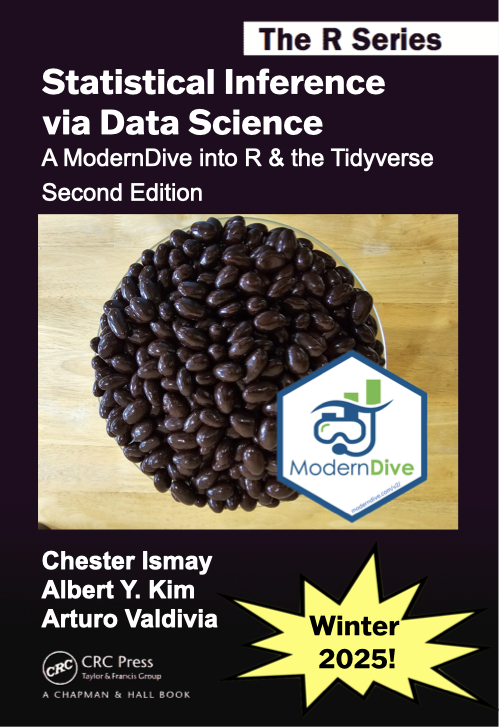
\includegraphics{images/logos/v2/v2_cover_2024-09-29.png}

This work by \href{https://chester.rbind.io/}{Chester Ismay}, \href{https://rudeboybert.rbind.io/}{Albert Y. Kim}, and \href{https://avaldivi6.github.io}{Arturo Valdivia} is licensed under a Creative Commons Attribution-NonCommercial-ShareAlike 4.0 International License.

\chapter*{Foreword}\label{foreword}


These are exciting times in statistics and data science education. (I am predicting this statement will continue to be true regardless of whether you are reading this foreword in 2025 or 2050.)
But (isn't there always a but?), as a statistics and data science educator, it can also feel a bit overwhelming to stay on top of all the new statistical, technological, and pedagogical innovations.
I find myself constantly asking, ``Am I teaching my students the correct content, with the relevant software, and in the most effective way?''
Before I make all of us feel lost at sea, let me point out how great a life raft I have found in \emph{ModernDive}.
In a sea of intro stats and data science textbooks, \emph{ModernDive} floats to the top of my list, and let me tell you why.
(Note my use of \emph{ModernDive} here refers to the book in its shortened title version.
This also matches up nicely with the \href{https://moderndive.com/images/logos/hex_blue_text.png}{neat hex sticker} Drs. Ismay, Kim, and Valdivia created for the cover of \emph{ModernDive}, too.)

\begin{center}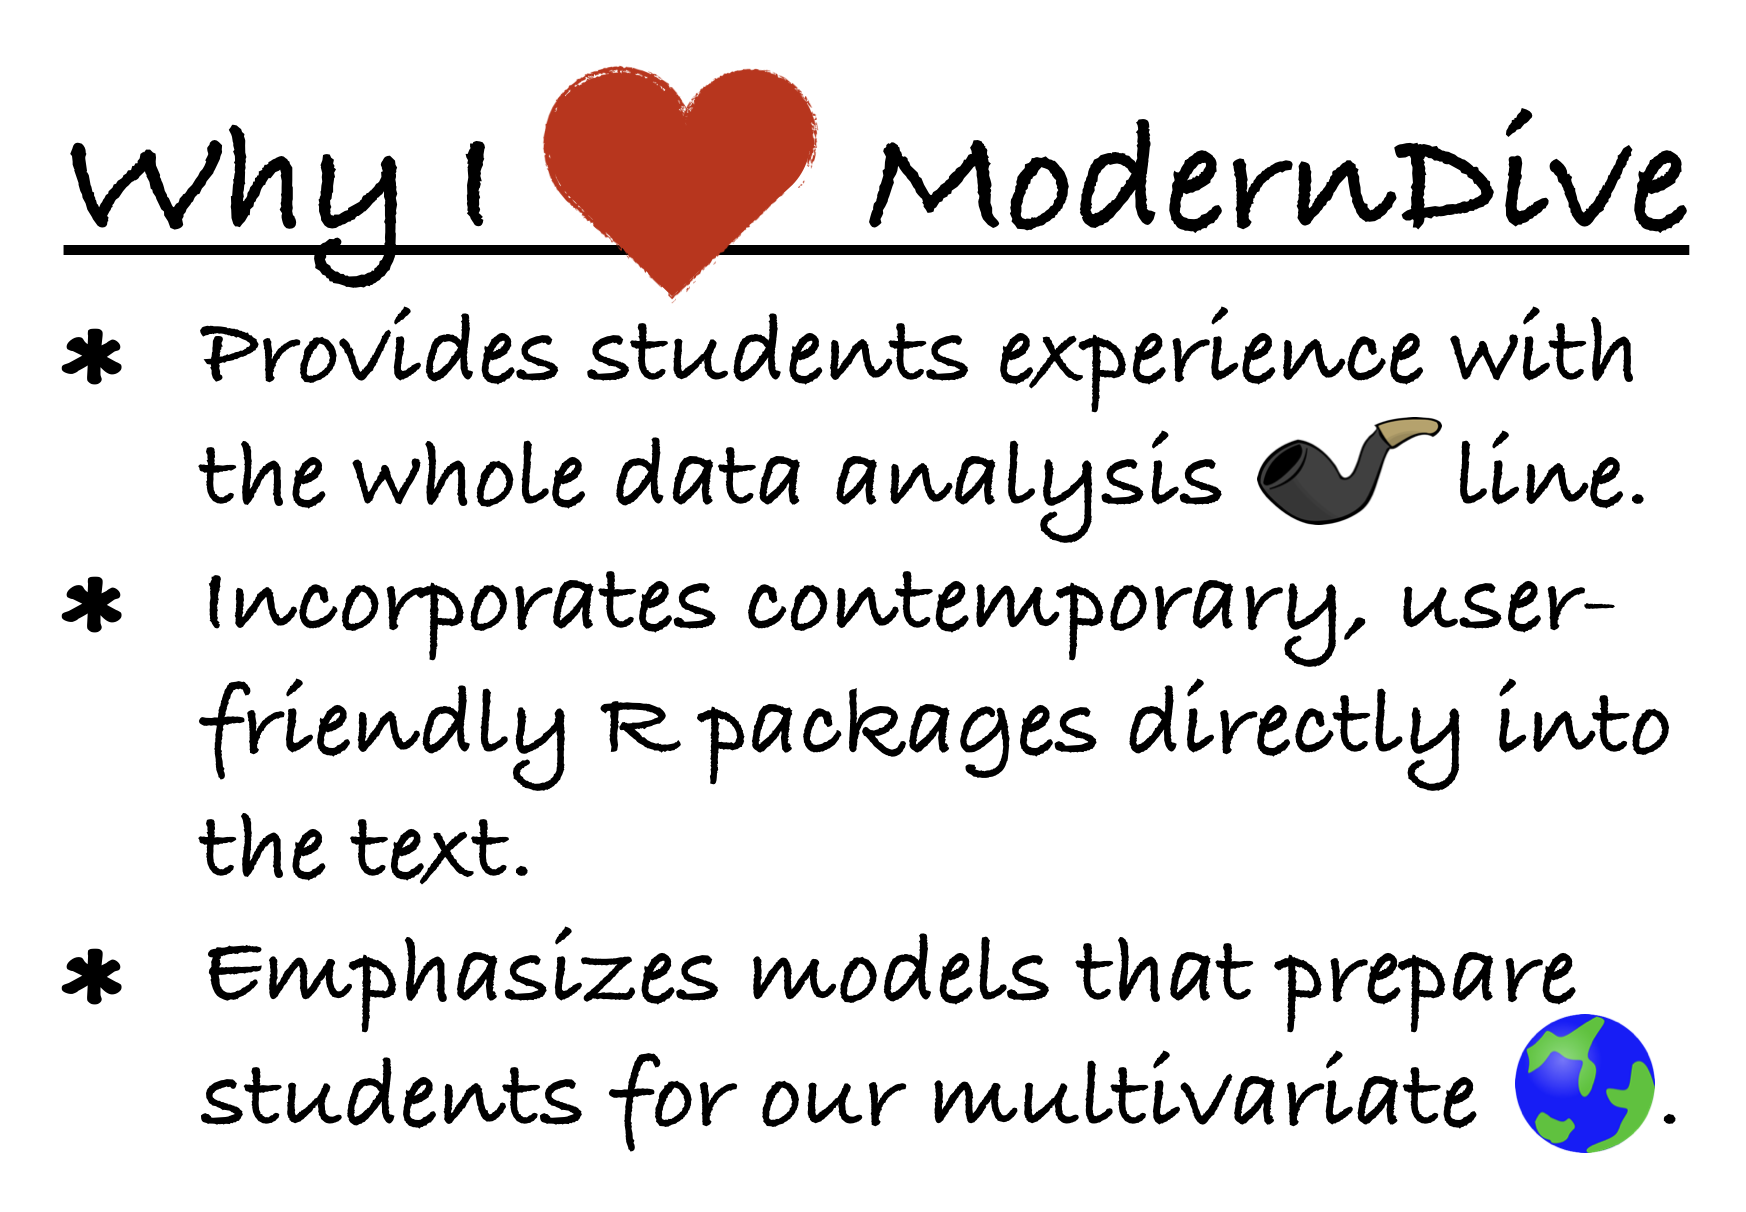
\includegraphics[width=0.7\linewidth]{images/ModernDive_heart} \end{center}

My favorite aspect of \emph{ModernDive}, if I must pick a favorite, is that students gain experience with the whole data analysis pipeline (see Figure \ref{fig:pipeline-figure}).
In particular, \emph{ModernDive} is one of the few intro stats and data science textbooks that teaches students how to wrangle data.
And, while data cleaning may not be as groovy as model building, it's often a prerequisite step!
The world is full of messy data and \emph{ModernDive} equips students to transform their data via the \texttt{dplyr} package.

Speaking of \texttt{dplyr}, students of \emph{ModernDive} are exposed to the \texttt{tidyverse} suite of R packages.
Designed with a common structure, \texttt{tidyverse} functions are written to be easy to learn and use.
And, since most intro stats and data science students are programming newbies, \emph{ModernDive} carefully walks the students through each new function it presents and provides frequent reinforcement through the many \emph{Learning checks} dispersed throughout the chapters.

Overall, \emph{ModernDive} includes wise choices for the placement of topics.
Starting with data visualization, \emph{ModernDive} gets students building \texttt{ggplot2} graphs early on and then continues to reinforce important concepts graphically throughout the book.
After moving through data wrangling and data importing, modeling plays a prominent role, with two chapters devoted to building regression models and a later chapter on inference for regression.
Lastly, statistical inference is presented first through a computational lens and then using a theory-based approach.
The \texttt{infer} package is used for both approaches and allows for easy comparisons between simulation-based and theory-based methods.

I first met two of the authors, Drs. Ismay and Kim, while attending their \href{https://www.causeweb.org/cause/uscots/uscots17/workshop/3}{workshop at the 2017 US Conference on Teaching Statistics}.
They pushed us as participants to put data first and to use computers, instead of math, as the engine for statistical inference.
That experience helped me add more data science concepts into my own intro stats course and introduced me to two really forward-thinking statistics and data science educators.
With the addition of Dr.~Valdivia on the second edition, it is exciting to see \emph{ModernDive} continue to develop and grow into such a wonderful, timely textbook.
The new edition includes even more engaging datasets, code updates that include the fancy base-pipe, more insights into inference, and materials that leverage newer functions from \texttt{infer} (make sure you check out the magical \texttt{fit()} function!).
With this refresh, \emph{ModernDive} continues to lead the pack as a truly contemporary approach to learning introductory statistics and data science.

I hope you have decided to dive on in!

\begin{flushright}
      \textit{Kelly S. McConville, Bucknell University}
      \end{flushright}

\chapter*{Preface}\label{preface}


\vspace{0.1in}


\includegraphics[width=\textwidth,height=0.1\textheight]{images/logos/Rlogo.png} \hfill       
\includegraphics[width=\textwidth,height=0.1\textheight]{images/logos/RStudio-Logo-Blue-Gradient.png}

\textbf{Help! I'm completely new to coding and I need to learn R and RStudio! What do I do?}

\vspace{0.1in}

If you're asking yourself this question, then you've come to the right place! Start with the ``Introduction for students'' section.

\begin{itemize}
\tightlist
\item
  \emph{Are you an instructor hoping to use this book in your courses? We recommend reading the ``Introduction for students'' section first. Then, read the ``Introduction for instructors'' section for more information on how to teach with this book.}
\item
  \emph{Are you looking to connect with and contribute to} ModernDive\emph{? Then, read the ``Connect and contribute'' section for information on how.}
\item
  \emph{Are you curious about the publishing of this book? Then, read the ``About this book'' section for more information on the open-source technology, in particular R Markdown and the bookdown package.}
\end{itemize}

\section*{Introduction for students}\label{introduction-for-students}


This book assumes no prerequisites: no algebra, no calculus, and no prior programming/coding experience. This is intended to be a gentle introduction to the practice of analyzing data and answering questions using data the way data scientists, statisticians, data journalists, and other researchers would.

We present a map of your upcoming journey in Figure \ref{fig:moderndive-figure}.



\begin{figure}[H]

{\centering 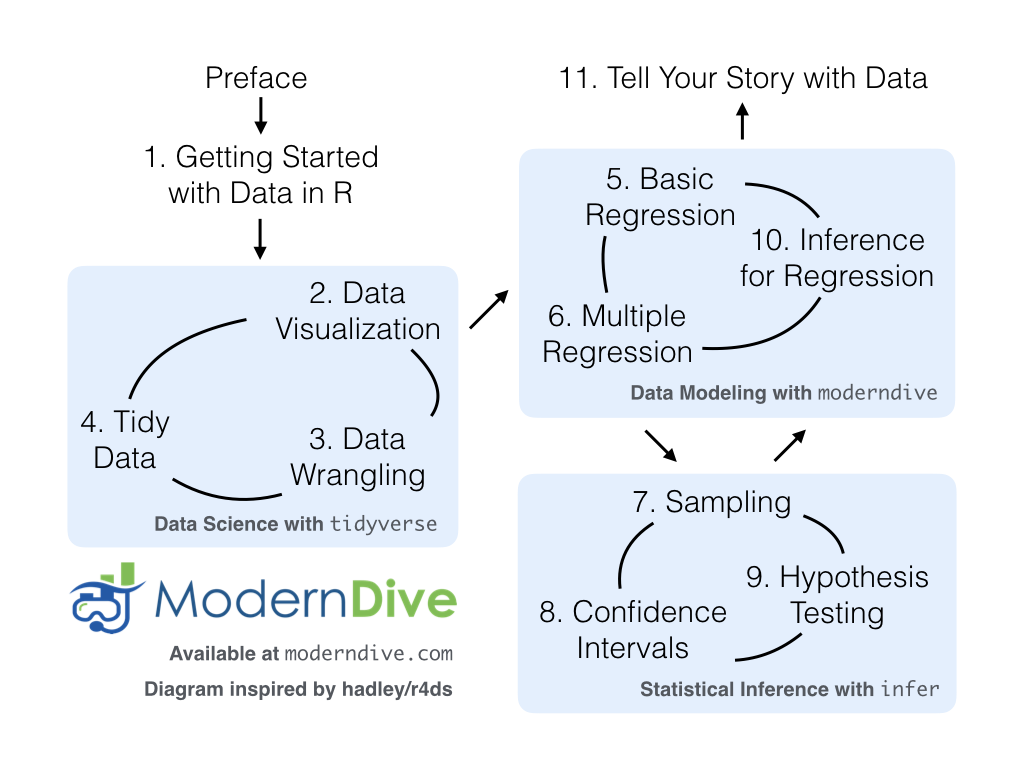
\includegraphics[width=\textwidth]{images/flowcharts/flowchart/flowchart.002} 

}

\caption{\emph{ModernDive} flowchart.}\label{fig:moderndive-figure}
\end{figure}

You'll first get started with data in Chapter \ref{getting-started} where you'll learn about the difference between R and RStudio, start coding in R, install and load your first R packages, and explore your first dataset: all domestic departure \texttt{flights} from a New York City airport in 2023. Then you'll cover the following three portions of this book (Parts 2 and 4 are combined into a single portion):

\begin{enumerate}
\def\labelenumi{\arabic{enumi}.}
\tightlist
\item
  Data science with \texttt{tidyverse}. You'll assemble your data science toolbox using \texttt{tidyverse} packages. In particular, you'll

  \begin{itemize}
  \tightlist
  \item
    Ch.\ref{viz}: Visualize data using the \texttt{ggplot2} package.
  \item
    Ch.\ref{wrangling}: Wrangle data using the \texttt{dplyr} package.
  \item
    Ch.\ref{tidy}: Learn about the concept of ``tidy'' data as a standardized data input and output format for all packages in the \texttt{tidyverse}. Furthermore, you'll learn how to import spreadsheet files into R using the \texttt{readr} package.
  \end{itemize}
\item
  Statistical/Data modeling with \texttt{moderndive}. Using these data science tools and helper functions from the \texttt{moderndive} package, you'll fit your first data models. In particular, you'll

  \begin{itemize}
  \tightlist
  \item
    Ch.\ref{regression}: Discover basic regression models with only one explanatory variable.
  \item
    Ch.\ref{multiple-regression}: Examine multiple regression models with more than one explanatory variable.
  \end{itemize}
\item
  Statistical inference with \texttt{infer}. Once again using your newly acquired data science tools, you'll unpack statistical inference using the \texttt{infer} package. In particular, you'll:

  \begin{itemize}
  \tightlist
  \item
    Ch.\ref{sampling}: Learn about the role that sampling variability plays in statistical inference and the role that sample size plays in this sampling variability.
  \item
    Ch.\ref{confidence-intervals}: Construct confidence intervals using bootstrapping.
  \item
    Ch.\ref{hypothesis-testing}: Conduct hypothesis tests using permutation.
  \end{itemize}
\item
  Statistical/Data modeling with \texttt{moderndive} (revisited): Armed with your understanding of statistical inference, you'll revisit and review the models you've constructed in Ch.\ref{regression} and Ch.\ref{multiple-regression}. In particular, you'll:

  \begin{itemize}
  \tightlist
  \item
    Ch.\ref{inference-for-regression}: Interpret confidence intervals and hypothesis tests in a regression setting.
  \end{itemize}
\end{enumerate}

We'll end with a discussion on what it means to ``tell your story with data'' in Chapter \ref{thinking-with-data} by presenting example case studies.\footnote{Note that you'll see different versions of the word ``ModernDive'' in this book:
  (1) \texttt{moderndive} refers to the R package.
  (2) \emph{ModernDive} is an abbreviated version of \emph{Statistical Inference via Data Science: A ModernDive into R and the Tidyverse}. It's essentially a nickname we gave the book.
  (3) ModernDive (without italics) corresponds to both the book and the corresponding R package together as an entity.}

\subsection*{What we hope you will learn from this book}\label{what-we-hope-you-will-learn-from-this-book}


We hope that by the end of this book, you'll have learned how to:

\begin{enumerate}
\def\labelenumi{\arabic{enumi}.}
\tightlist
\item
  Use R and the \texttt{tidyverse} suite of R \emph{packages} for data science.
\item
  Fit your first \emph{models} to data, using a method known as \emph{linear regression}.
\item
  Perform \emph{statistical inference} using \emph{sampling}, \emph{confidence intervals}, and \emph{hypothesis tests}.
\item
  \emph{Tell your story with data} using these tools.
\end{enumerate}

What do we mean by data stories? We mean any analysis involving data that engages the reader in answering questions with careful visuals and thoughtful discussion. Further discussions on data stories can be found in the blog post \href{https://www.thinkwithgoogle.com/marketing-resources/data-measurement/tell-meaningful-stories-with-data/}{``Tell a Meaningful Story With Data.''}

Over the course of this book, you will develop your ``data science toolbox,'' equipping yourself with tools such as data visualization, data formatting, data wrangling, and statistical/data modeling using regression.

In particular, this book will lean heavily on data visualization. In today's world, we are bombarded with graphics that attempt to convey ideas. We will explore what makes a good graphic and what the standard ways are used to convey relationships within data. In general, we'll use visualization as a way of building almost all of the ideas in this book.

To impart the statistical lessons of this book, we have intentionally minimized the number of mathematical formulas used. Instead, you'll develop a conceptual understanding of statistics using data visualization and computer simulations. We hope this is a more intuitive experience than the way statistics has traditionally been taught in the past and how it is commonly perceived.

Finally, you'll learn the importance of literate programming. \index{literate programming} By this we mean you'll learn how to write code that is useful not just for a computer to execute, but also for readers to understand exactly what your analysis is doing and how you did it. This is part of a greater effort to encourage reproducible research (see the ``Reproducible research'' subsection in this Preface for more details). Hal Abelson \index{Abelson, Hal} coined the phrase that we will follow throughout this book:

\begin{quote}
Programs must be written for people to read, and only incidentally for machines to execute.
\end{quote}

We understand that there may be challenging moments as you learn to program. Both of us continue to struggle and find ourselves often using web searches to find answers and reach out to colleagues for help. In the long run though, we all can solve problems faster and more elegantly via programming. We wrote this book as our way to help you get started and you should know that there is a huge community of R users that are happy to help everyone along as well. This community exists in particular on the internet on various forums and websites such as \href{https://stackoverflow.com/}{stackoverflow.com}.

\subsection*{Data/science pipeline}\label{datascience-pipeline}


You may think of statistics as just being a bunch of numbers. We commonly hear the phrase ``statistician'' when listening to broadcasts of sporting events. Statistics (in particular, data analysis), in addition to describing numbers like with baseball batting averages, plays a vital role in all of the sciences. \index{statistics}

You'll commonly hear the phrase ``statistically significant'' thrown around in the media. You'll see articles that say, ``Science now shows that chocolate is good for you.'' Underpinning these claims is data analysis. \index{data analysis} By the end of this book, you'll be able to better understand whether these claims should be trusted or whether we should be wary. Inside data analysis are many sub-fields that we will discuss throughout this book (though not necessarily in this order):

\begin{itemize}
\tightlist
\item
  data collection
\item
  data wrangling
\item
  data visualization
\item
  statistical modeling
\item
  inference
\item
  correlation and regression
\item
  interpretation of results
\item
  data communication/storytelling
\end{itemize}

These sub-fields are summarized in what Garrett Grolemund \index{Grolemund, Garrett} and Hadley Wickham \index{Wickham, Hadley} have previously termed the \href{http://r4ds.had.co.nz/explore-intro.html}{``data/science pipeline''} in Figure \ref{fig:pipeline-figure}.

\begin{figure}[H]

{\centering 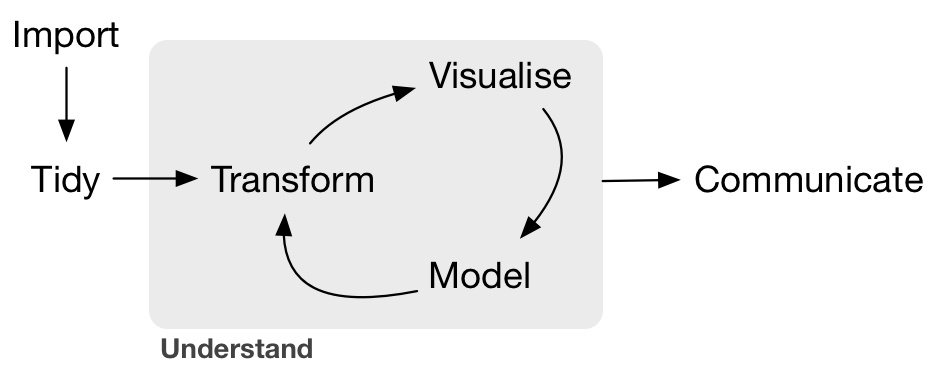
\includegraphics[width=1\linewidth,height=1\textheight]{images/r4ds/data_science_pipeline} 

}

\caption{Data/science pipeline.}\label{fig:pipeline-figure}
\end{figure}

We will begin by digging into the grey \textbf{Understand} portion of the cycle with data visualization, then with a discussion on what is meant by tidy data and data wrangling, and then conclude by talking about interpreting and discussing the results of our models via \textbf{Communication}. These steps are vital to any statistical analysis. But, why should you care about statistics?

There's a reason that many fields require a statistics course. Scientific knowledge grows through an understanding of statistical significance and data analysis. You needn't be intimidated by statistics. It's not the beast that it used to be and, paired with computation, you'll see how reproducible research in the sciences particularly increases scientific knowledge.

\subsection*{Reproducible research}\label{reproducible-research}


\begin{quote}
The most important tool is the \emph{mindset}, when starting, that the end product will be reproducible. -- Keith Baggerly
\end{quote}

\index{Baggerly, Keith}

Another goal of this book is to help readers understand the importance of reproducible analyses. The hope is to get readers into the habit of making their analyses reproducible from the very beginning. This means we'll be trying to help you build new habits. This will take practice and be difficult at times. You'll see just why it is so important for you to keep track of your code and document it well to help yourself later and any potential collaborators as well.

Copying and pasting results from one program into a word processor is not an ideal way to conduct efficient and effective scientific research. It's much more important for time to be spent on data collection and data analysis and not on copying and pasting plots back and forth across a variety of programs.

In traditional analyses, if an error was made with the original data, we'd need to step through the entire process again: recreate the plots and copy-and-paste all of the new plots and our statistical analysis into our document. This is error prone and a frustrating use of time. We want to help you to get away from this tedious activity so that we can spend more time doing science.

\begin{quote}
We are talking about \emph{computational} reproducibility. -- Yihui Xie
\end{quote}

\index{Xie, Yihui}

Reproducibility means a lot of things in terms of different scientific fields. Are experiments conducted in a way that another researcher could follow the steps and get similar results? In this book, we will focus on what is known as \textbf{computational reproducibility}. \index{computational reproducibility} This refers to being able to pass all of one's data analysis, datasets, and conclusions to someone else and have them get exactly the same results on their machine. This allows for time to be spent interpreting results and considering assumptions instead of the more error prone way of starting from scratch or following a list of steps that may be different from machine to machine.

\subsection*{Final note for students}\label{final-note-for-students}


At this point, if you are interested in instructor perspectives on this book, ways to contribute and collaborate, or the technical details of this book's construction and publishing, then continue with the rest of the chapter. Otherwise, let's get started with R and RStudio in Chapter \ref{getting-started}!

\section*{Introduction for instructors}\label{introduction-for-instructors}


\subsection*{Resources}\label{resources}


Here are some resources to help you use \emph{ModernDive}:

\begin{enumerate}
\def\labelenumi{\arabic{enumi}.}
\tightlist
\item
  We've included review questions posed as \emph{Learning checks}. You can find all the solutions to all \emph{Learning checks} in the Appendices of the online version of the book. The Appendices start at \url{https://moderndive.com/v2/appendixa}.
\item
  Dr.~Jenny Smetzer and Albert Y. Kim have written a series of labs and problem sets. You can find them at \url{https://moderndive.com/labs}.
\item
  You can see the webpages for two courses that use \emph{ModernDive}:

  \begin{itemize}
  \tightlist
  \item
    Smith College ``SDS192 Introduction to Data Science'': \url{https://rudeboybert.github.io/SDS192/}.
  \item
    Smith College ``SDS220 Introduction to Probability and Statistics'': \url{https://rudeboybert.github.io/SDS220/}.
  \end{itemize}
\end{enumerate}

\subsection*{Why did we write this book?}\label{why-did-we-write-this-book}


This book is inspired by

\begin{itemize}
\tightlist
\item
  \emph{Mathematical Statistics with Resampling and R} \citep{hester2011}
\item
  \emph{OpenIntro: Intro Stat with Randomization and Simulation} \citep{isrs2014}
\item
  \emph{R for Data Science} \citep{rds2016}
\end{itemize}

The first book, designed for upper-level undergraduates and graduate students, provides an excellent resource on how to use resampling to impart statistical concepts like sampling distributions using computation instead of large-sample approximations and other mathematical formulas. The last two books are free options for learning about introductory statistics and data science, providing an alternative to the many traditionally expensive introductory statistics textbooks.

When looking over the introductory statistics textbooks that currently exist, we found there wasn't one that incorporated many newly developed R packages directly into the text, in particular the many packages included in the \href{http://tidyverse.org/}{\texttt{tidyverse}} set of packages, such as \texttt{ggplot2}, \texttt{dplyr}, \texttt{tidyr}, and \texttt{readr} that will be the focus of this book's first part on ``Data Science with \texttt{tidyverse}.''

Additionally, there wasn't an open-source and easily reproducible textbook available that exposed new learners to all four of the learning goals we listed in the ``Introduction for students'' subsection. We wanted to write a book that could develop theory via computational techniques and help novices master the R language in doing so.

\subsection*{Who is this book for?}\label{who-is-this-book-for}


This book is intended for instructors of traditional introductory statistics classes using RStudio, who would like to inject more data science topics into their syllabus. RStudio can be used in either the server version or the desktop version. (This is discussed further in Subsection \ref{installing}.) We assume that students taking the class will have no prior algebra, no calculus, nor programming/coding experience.

Here are some principles and beliefs we kept in mind while writing this text. If you agree with them, this is the book for you.

\begin{enumerate}
\def\labelenumi{\arabic{enumi}.}
\tightlist
\item
  \textbf{Blur the lines between lecture and lab}

  \begin{itemize}
  \tightlist
  \item
    With increased availability and accessibility of laptops and open-source non-proprietary statistical software, the strict dichotomy between lab and lecture can be loosened.
  \item
    It's much harder for students to understand the importance of using software if they only use it once a week or less. They forget the syntax in much the same way someone learning a foreign language forgets the grammar rules. Frequent reinforcement is key.
  \end{itemize}
\item
  \textbf{Focus on the entire data/science research pipeline}

  \begin{itemize}
  \tightlist
  \item
    We believe that the entirety of Grolemund and Wickham's \href{http://r4ds.had.co.nz/introduction.html}{data/science pipeline} \index{data science pipeline} as seen in Figure \ref{fig:pipeline-figure} should be taught.
  \item
    We heed George Cobb's call to \href{https://arxiv.org/abs/1507.05346}{``minimize prerequisites to research''}: \index{Cobb, George} students should be answering questions with data as soon as possible.
  \end{itemize}
\item
  \textbf{It's all about the data}

  \begin{itemize}
  \tightlist
  \item
    We leverage R packages for rich, real, and realistic datasets that at the same time are easy-to-load into R, such as the \texttt{nycflights23} and \texttt{fivethirtyeight} packages.
  \item
    We believe that \href{http://escholarship.org/uc/item/84v3774z}{data visualization is a ``gateway drug'' for statistics} and that the grammar of graphics as implemented in the \texttt{ggplot2} package is the best way to impart such lessons. However, we often hear: ``You can't teach \texttt{ggplot2} for data visualization in intro stats!'' We, like \index{Robinson, David} \href{http://varianceexplained.org/r/teach_ggplot2_to_beginners/}{David Robinson}, are much more optimistic and have found our students have been largely successful in learning it.
  \item
    \texttt{dplyr} has made data wrangling much more \href{http://chance.amstat.org/2015/04/setting-the-stage/}{accessible} to novices, and hence much more interesting datasets can be explored.
  \end{itemize}
\item
  \textbf{Use simulation/resampling to introduce statistical inference, not probability/mathematical formulas}

  \begin{itemize}
  \tightlist
  \item
    Instead of using formulas, large-sample approximations, and probability tables, we teach statistical concepts using simulation-based inference.
  \item
    This allows for a de-emphasis of traditional probability topics, freeing up room in the syllabus for other topics. Bridges to these mathematical concepts are given as well to help with relation of these traditional topics with more modern approaches.
  \end{itemize}
\item
  \textbf{Don't fence off students from the computation pool, throw them in!}

  \begin{itemize}
  \tightlist
  \item
    Computing skills are essential to working with data in the 21st century. Given this fact, we feel that to shield students from computing is to ultimately do them a disservice.
  \item
    We are not teaching a course on coding/programming per se, but rather just enough of the computational and algorithmic thinking necessary for data analysis.
  \end{itemize}
\item
  \textbf{Complete reproducibility and customizability}

  \begin{itemize}
  \tightlist
  \item
    We are frustrated when textbooks give examples, but not the source code and the data itself. We give you the source code for all examples as well as the whole book! While we have made choices to occasionally hide the code that produces more complicated figures, reviewing the book's GitHub repository will provide you with all the code (see below).
  \item
    Ultimately the best textbook is one you've written yourself. You know best your audience, their background, and their priorities. You know best your own style and the types of examples and problems you like best. Customization is the ultimate end. We encourage you to take what we've provided and make it work for your own needs. For more about how to make this book your own, see ``About this book'' later in this Preface.
  \end{itemize}
\end{enumerate}

\section*{Connect and contribute}\label{connect-and-contribute}


If you would like to connect with ModernDive, check out the following links:

\begin{itemize}
\tightlist
\item
  If you would like to receive periodic updates about ModernDive (roughly every 6 months), please sign up for our \href{http://eepurl.com/cBkItf}{mailing list}.
\item
  We're on X (formerly Twitter) at \url{https://x.com/ModernDive}.
\end{itemize}

If you would like to contribute to \emph{ModernDive}, there are many ways! We would love your help and feedback to make this book as great as possible! For example, if you find any errors, typos, or areas for improvement, then please post an issue on our \href{https://github.com/moderndive/moderndive_book/issues}{GitHub issues} \index{GitHub issues} page. If you are familiar with GitHub and would like to contribute, see the ``About this book'' section.

\section*{Acknowledgements}\label{acknowledgements}


The authors would like to thank \href{https://github.com/nsonneborn}{Nina Sonneborn}, \href{https://alison.rbind.io/}{Dr.~Alison Hill}, \href{https://twitter.com/rhobott?lang=en}{Kristin Bott}, Dr.~Jenny Smetzer, \href{https://www.smith.edu/academics/faculty/katherine-kinnaird}{Prof.~Katherine Kinnaird}, and the participants of our \href{https://www.causeweb.org/cause/uscots/uscots17/workshop/3}{2017} and \href{https://www.causeweb.org/cause/uscots/uscots19/workshop/4}{2019} USCOTS workshops for their feedback and suggestions. We'd also like to thank \href{https://twitter.com/andrewheiss}{Dr.~Andrew Heiss} for contributing nearly all of Subsection \ref{tips-code} on ``Errors, warnings, and messages,'' \href{https://github.com/echasnovski}{Evgeni Chasnovski} for creating the \texttt{geom\_parallel\_slopes()} extension to the \texttt{ggplot2} package for plotting parallel slopes models, and Smith College Statistical \& Data Sciences students \href{https://github.com/Starryz}{Starry Zhou} and \href{https://github.com/mariumtapal}{Marium Tapal} for their many edits to the book. A special thanks goes to Dr.~Jude Weinstein-Jones, co-founder of \href{https://www.learningscientists.org}{The Learning Scientists}, for their extensive feedback. Much appreciation also goes to \href{https://jasminloerchner.de/}{Jasmin Lörchner} for her thorough read, continued support, and thoughtful edits for the second edition of this book!

We were honored to have \href{https://mcconville.rbind.io/}{Dr.~Kelly S. McConville} write the \hyperref[foreword]{Foreword} of both editions of the book. Dr.~McConville is a pioneer in statistics education and was a source of great inspiration to both of us as we continued to update the book to get it to its current form. Thanks additionally to the \href{https://github.com/moderndive/ModernDive_book/graphs/contributors}{continued contributions by members of the community} to the book on GitHub and to the many individuals that have recommended this book to others. We are so very appreciative of all of you!

Lastly, a special shout out to any student who has ever taken a class with us at Pacific University, Reed College, Middlebury College, Amherst College, Smith College, or Indiana University. We couldn't have made this book without you!

\section*{About this book}\label{about-the-book}


This book was written using RStudio's \href{https://bookdown.org/}{bookdown} package\index{R packages!bookdown} by \index{Xie, Yihui}Yihui Xie\citep{R-bookdown}. This package simplifies the publishing of books by having all content written in \index{R Markdown} \href{http://rmarkdown.rstudio.com/html_document_format.html}{R Markdown}. The bookdown/R Markdown source code for all versions of ModernDive is available on GitHub:

\begin{itemize}
\tightlist
\item
  \textbf{Latest online version} The most up-to-date release:

  \begin{itemize}
  \tightlist
  \item
    Version 2.0.0 released on September 24, 2024 (\href{https://github.com/moderndive/moderndive_book/releases/tag/v2.0.0}{source code})
  \item
    Available at \url{https://moderndive.com/v2/}
  \end{itemize}
\item
  \textbf{Print second edition} The CRC Press print edition is what you are reading! It corresponds to Version 2.0.0. We welcomed Dr.~Arturo Valdivia as a co-author for this edition. His deep knowledge of statistics and superb teaching experience have been invaluable in improving the book. Here is a summary of what was updated from v1.0.0 to v2.0.0 (first print edition to second print edition). Additional information about changes to the book over time are available on our GitHub page \href{https://github.com/moderndive/ModernDive_book/blob/v2/NEWS.md}{here}.

  \begin{itemize}
  \tightlist
  \item
    \textbf{Updated Datasets and Code:} Replaced datasets (\texttt{promotions}, \texttt{evals}, and \texttt{pennies}) with new ones (\texttt{un\_member\_states\_2024}, \texttt{spotify\_sample}, and \texttt{almonds\_bowl}). Adopted the \texttt{nycflights23} package instead of \texttt{nycflights13} and introduced the base R pipe (\texttt{\textbar{}\textgreater{}}) instead of the tidyverse pipe (\texttt{\%\textgreater{}\%}). Also incorporated \texttt{envoy\_flights} and \texttt{early\_january\_2023\_weather} in the \texttt{moderndive} package.
  \item
    \textbf{Content Reorganization:} Restructured sections in Chapters 7 and 10 for improved readability. Moved ``Model Selection'' from Chapter 6 to Chapter 10 and split it into two new subsections as per suggestions.
  \item
    \textbf{Enhanced Theoretical Discussions:} Improved theory-based discussions in Chapters 7, 8, 10, and 11, and added sections to better connect statistical inference based on reviewer feedback.
  \item
    \textbf{New Examples and Functions:} Introduced \texttt{coffee\_quality} and \texttt{old\_faithful\_2024} datasets with examples in Chapter 10, added use of the \texttt{fit()} function from the \texttt{infer} package for simulation-based inference with multiple linear regression, and incorporated the \texttt{infer} package into Chapter 11.
  \item
    \textbf{Code Enhancements and Clarifications:} Standardized code to use \texttt{\textbar{}\textgreater{}}, addressed warnings for \texttt{group\_by()}, and added \texttt{relocate()} to Chapter 3.
  \item
    \textbf{Revamped Learning Checks:}: Updated and designed new Learning checks throughout the book to better assess student understanding.
  \end{itemize}
\item
  \textbf{Print first edition} The CRC Press \href{https://www.routledge.com/Statistical-Inference-via-Data-Science-A-ModernDive-into-R-and-the-Tidyverse/Ismay-Kim/p/book/9780367409821}{print edition} of \emph{ModernDive} corresponds to Version 1.1.0 (with some typos fixed). Available at \url{https://moderndive.com/}.
\item
  \textbf{Previous online versions} Older versions that may be out of date:

  \begin{itemize}
  \tightlist
  \item
    \href{previous_versions/v1.0.0/index.html}{Version 1.0.0} released on November 25, 2019 (\href{https://github.com/moderndive/ModernDive_book/releases/tag/v1.0.0}{source code})
  \item
    \href{previous_versions/v0.6.1/index.html}{Version 0.6.1} released on August 28, 2019 (\href{https://github.com/moderndive/ModernDive_book/releases/tag/v0.6.1}{source code})
  \item
    \href{previous_versions/v0.6.0/index.html}{Version 0.6.0} released on August 7, 2019 (\href{https://github.com/moderndive/moderndive_book/releases/tag/v0.6.0}{source code})
  \item
    \href{previous_versions/v0.5.0/index.html}{Version 0.5.0} released on February 24, 2019 (\href{https://github.com/moderndive/moderndive_book/releases/tag/v0.5.0}{source code})
  \item
    \href{previous_versions/v0.4.0/index.html}{Version 0.4.0} released on July 21, 2018 (\href{https://github.com/moderndive/moderndive_book/releases/tag/v0.4.0}{source code})
  \item
    \href{previous_versions/v0.3.0/index.html}{Version 0.3.0} released on February 3, 2018 (\href{https://github.com/moderndive/moderndive_book/releases/tag/v0.3.0}{source code})
  \item
    \href{previous_versions/v0.2.0/index.html}{Version 0.2.0} released on August 2, 2017 (\href{https://github.com/moderndive/moderndive_book/releases/tag/v0.2.0}{source code})
  \item
    \href{previous_versions/v0.1.3/index.html}{Version 0.1.3} released on February 9, 2017 (\href{https://github.com/moderndive/moderndive_book/releases/tag/v0.1.3}{source code})
  \item
    \href{previous_versions/v0.1.2/index.html}{Version 0.1.2} released on January 22, 2017 (\href{https://github.com/moderndive/moderndive_book/releases/tag/v0.1.2}{source code})
  \end{itemize}
\end{itemize}

Could this be a new paradigm for textbooks? Instead of the traditional model of textbook companies publishing updated \emph{editions} of the textbook every few years, we apply a software design influenced model of publishing more easily updated \emph{versions}. We can then leverage open-source communities of instructors and developers for ideas, tools, resources, and feedback. As such, we welcome your GitHub pull requests.

Finally, since this book is under a \href{https://creativecommons.org/licenses/by-nc-sa/4.0/}{Creative Commons Attribution - NonCommercial - ShareAlike 4.0 license}, feel free to modify the book as you wish for your own non-commercial needs, but please list the authors at the top of \texttt{index.Rmd} as: ``Chester Ismay, Albert Y. Kim, Arturo Valdivia, and YOU!''

\newpage

\section*{Versions of R packages used}\label{versions-of-r-packages-used}


If you'd like your output on your computer to match up exactly with the output presented throughout the book, you may want to use the exact versions of the packages that we used. You can find a full listing of these packages and their versions below. This likely won't be relevant for novices, but we included it for reproducibility.

If you are seeing different results than what is in the book, we recommend installing the exact version of the packages we used. This can be done by first installing the \texttt{remotes} package via \texttt{install.packages("remotes")}. Then, use \texttt{install\_version()} replacing the \texttt{package} argument with the package name in quotes and the \texttt{version} argument with the particular version number to install such as

\begin{Shaded}
\begin{Highlighting}[]
\NormalTok{remotes}\SpecialCharTok{::}\FunctionTok{install\_version}\NormalTok{(}\AttributeTok{package =} \StringTok{"moderndive"}\NormalTok{, }\AttributeTok{version =} \StringTok{"0.6.1"}\NormalTok{)}
\end{Highlighting}
\end{Shaded}

\begingroup\fontsize{9}{11}\selectfont

\begin{longtable}[t]{ll}
\toprule
package & version\\
\midrule
bookdown & 0.40\\
broom & 1.0.7\\
dplyr & 1.1.4\\
fivethirtyeight & 0.6.2\\
forcats & 1.0.0\\
gapminder & 1.0.0\\
ggplot2 & 3.5.1\\
ggplot2movies & 0.0.1\\
ggrepel & 0.9.5\\
gridExtra & 2.3\\
infer & 1.0.7.9000\\
ISLR2 & 1.3-2\\
janitor & 2.2.0\\
kableExtra & 1.4.0\\
knitr & 1.48\\
lubridate & 1.9.3\\
moderndive & 0.7.0\\
mvtnorm & 1.2-6\\
nycflights23 & 0.1.0\\
patchwork & 1.3.0\\
purrr & 1.0.2\\
readr & 2.1.5\\
scales & 1.3.0\\
sessioninfo & 1.2.2\\
stringr & 1.5.1\\
tibble & 3.2.1\\
tidyr & 1.3.1\\
tidyverse & 2.0.0\\
viridis & 0.6.5\\
viridisLite & 0.4.2\\
\bottomrule
\end{longtable}
\endgroup{}

\chapter*{About the authors}\label{about-the-authors}


\begin{longtable}[]{@{}
  >{\centering\arraybackslash}p{(\columnwidth - 4\tabcolsep) * \real{0.3333}}
  >{\centering\arraybackslash}p{(\columnwidth - 4\tabcolsep) * \real{0.3333}}
  >{\centering\arraybackslash}p{(\columnwidth - 4\tabcolsep) * \real{0.3333}}@{}}
\toprule\noalign{}
\begin{minipage}[b]{\linewidth}\centering
Chester Ismay
\end{minipage} & \begin{minipage}[b]{\linewidth}\centering
Albert Y. Kim
\end{minipage} & \begin{minipage}[b]{\linewidth}\centering
Arturo Valdivia
\end{minipage} \\
\midrule\noalign{}
\endhead
\bottomrule\noalign{}
\endlastfoot

\includegraphics[width=0.33\textwidth,height=\textheight]{images/ismay2024.jpg} & 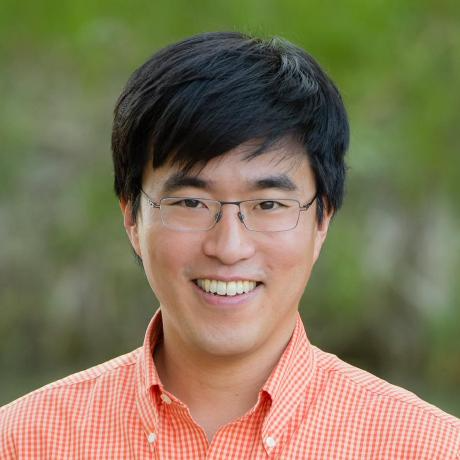
\includegraphics[width=0.33\textwidth,height=\textheight]{images/kim.png} & 
\includegraphics[width=0.33\textwidth,height=\textheight]{images/valdivia.png} \\
\end{longtable}

\textbf{Chester Ismay} is Vice President of Data and Automation at MATE Seminars and is a freelance data science consultant and instructor. He also teaches in the Center for Executive and Professional Education at Portland State University. He completed his PhD in statistics from Arizona State University in 2013. He has previously worked in a variety of roles including as an actuary at Scottsdale Insurance Company (now Nationwide E\&S/Specialty) and at Ripon College, Reed College, and Pacific University. He has experience working in online education and was previously a Data Science Evangelist at DataRobot, where he led data science, machine learning, and data engineering in-person and virtual workshops for DataRobot University. In addition to his work for \emph{ModernDive}, he also contributed as initial developer of the \href{https://cran.r-project.org/package=infer}{\texttt{infer}} R package and is author and maintainer of the \href{https://github.com/ismayc/thesisdown}{\texttt{thesisdown}} R package.

\begin{itemize}
\tightlist
\item
  Webpage: \url{https://chester.rbind.io/}
\item
  GitHub: \url{https://github.com/ismayc}
\end{itemize}

\textbf{Albert Y.~Kim} is an Associate Professor of Statistical \& Data Sciences at Smith College in Northampton, MA, USA. He completed his PhD in statistics at the University of Washington in 2011. Previously he worked in the Search Ads Metrics Team at Google Inc.~as well as at Reed, Middlebury, and Amherst Colleges. In addition to his work for \emph{ModernDive}, he is a co-author of the \href{https://cran.r-project.org/package=resampledata}{\texttt{resampledata}} and \href{https://cran.r-project.org/package=SpatialEpi}{\texttt{SpatialEpi}} R packages. Both Dr.~Kim and Dr.~Ismay, along with \href{https://github.com/jchunn}{Jennifer Chunn}, are co-authors of the \href{https://fivethirtyeight-r.netlify.app/}{\texttt{fivethirtyeight}} package of code and datasets published by the data journalism website \href{https://fivethirtyeight.com/}{FiveThirtyEight.com}.

\begin{itemize}
\tightlist
\item
  Webpage: \url{http://rudeboybert.rbind.io/}
\item
  GitHub: \url{https://github.com/rudeboybert}
\end{itemize}

\textbf{Arturo Valdivia} is a Senior Lecturer in the Department of Statistics at Indiana University, Bloomington.
He earned his PhD in Statistics from Arizona State University in 2013.
His research interests focus on statistical education, exploring innovative approaches to help students grasp complex ideas with clarity.
Over his career, he has taught a wide range of statistics courses, from introductory to advanced levels, to more than 1,800 undergraduate students and over 900 graduate students pursuing master's and Ph.D.~programs in statistics, data science, and other disciplines. In recognition of his teaching excellence, he received Indiana University's Trustees Teaching Award in 2023.

\begin{itemize}
\tightlist
\item
  Webpage: \url{https://avaldivi6.github.io}
\item
  GitHub: \url{https://github.com/avaldivi6}
\end{itemize}

\mainmatter

\chapter{Getting Started with Data in R}\label{getting-started}

Before we can start exploring data in R, there are some key concepts to understand first:

\begin{enumerate}
\def\labelenumi{\arabic{enumi}.}
\tightlist
\item
  What are R and RStudio?
\item
  How do I code in R?
\item
  What are R packages?
\end{enumerate}

We'll introduce these concepts in the upcoming Sections \ref{r-rstudio}-\ref{packages}. If you are already somewhat familiar with these concepts, feel free to skip to Section \ref{nycflights} where we'll introduce our first dataset: all domestic flights departing one of the three main New York City (NYC) airports in 2023. This is a dataset we will explore in depth for much of the rest of this book.

\section{What are R and RStudio?}\label{r-rstudio}

Throughout this book, we will assume that you are using R via RStudio. First time users often confuse the two. At its simplest, R is like a car's engine\index{R} while RStudio is like a car's dashboard\index{RStudio} as illustrated in Figure \ref{fig:R-vs-RStudio-1}.

\begin{figure}[H]

{\centering 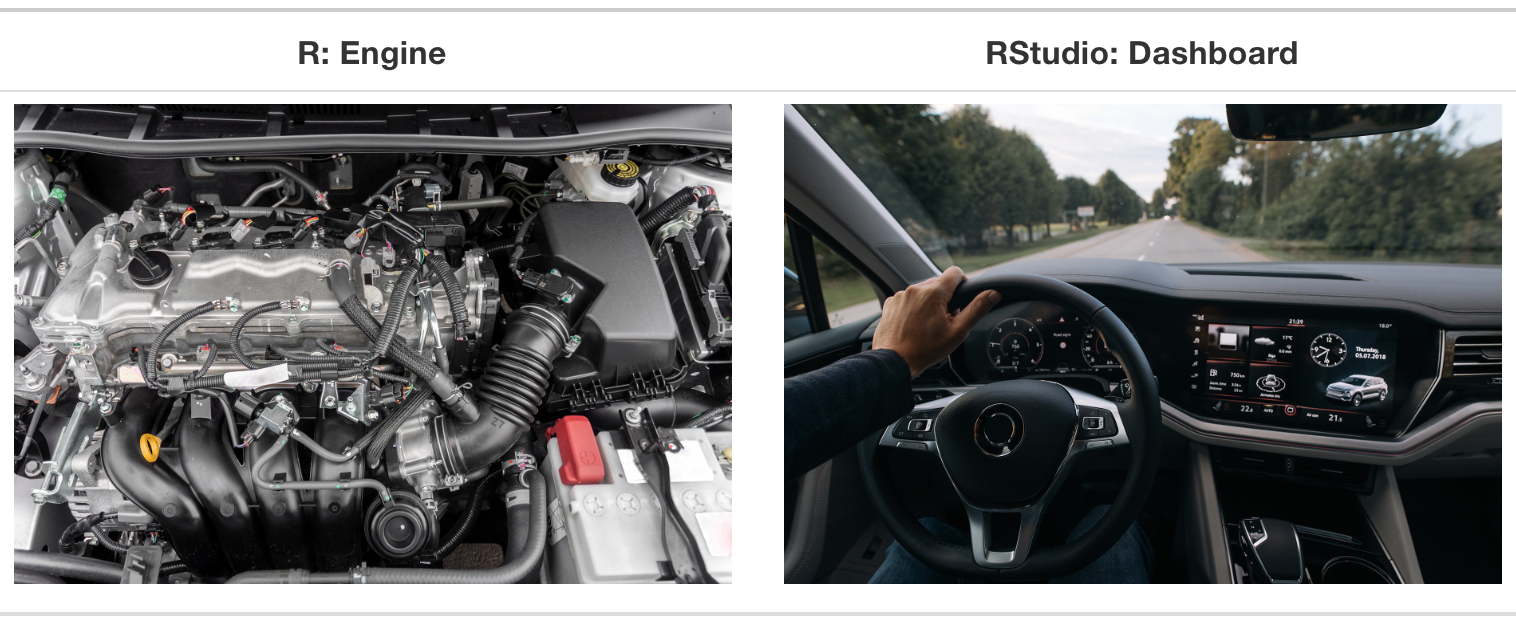
\includegraphics[width=0.95\linewidth]{images/shutterstock/R_vs_RStudio_1} 

}

\caption{Analogy of difference between R and RStudio.}\label{fig:R-vs-RStudio-1}
\end{figure}

More precisely, R is a programming language that runs computations, while RStudio is an \emph{integrated development environment (IDE)} that provides an interface by adding many convenient features and tools. So just as the way of having access to a speedometer, rear-view mirrors, and a navigation system makes driving much easier, using RStudio's interface makes using R much easier as well.

\subsection{Installing R and RStudio}\label{installing}

\begin{quote}
\textbf{Note about RStudio Server or RStudio Cloud}: If your instructor has provided you with a link and access to RStudio Server or RStudio Cloud, then you can skip this section. We do recommend after a few months of working on RStudio Server/Cloud that you return to these instructions to install this software on your own computer though.
\end{quote}

You will first need to download and install both R and RStudio (Desktop version) on your computer. It is important that you install R first and then install RStudio.

\begin{enumerate}
\def\labelenumi{\arabic{enumi}.}
\tightlist
\item
  \textbf{You must do this first:} Download and install R by going to \url{https://cloud.r-project.org/}. \index{R!installation}

  \begin{itemize}
  \tightlist
  \item
    If you are a Windows user: Click on ``Download R for Windows'', then click on ``base'', then click on the Download link.
  \item
    If you are macOS user: Click on ``Download R for macOS'', then under ``Latest release:'' click on R-X.X.X.pkg, where R-X.X.X is the version number. For example, the latest version of R as of May 24, 2024 was R-4.4.0.
  \item
    If you are a Linux user: Click on ``Download R for Linux'' and choose your distribution for more information on installing R for your setup.
  \end{itemize}
\item
  \textbf{You must do this second:} Download and install RStudio at \url{https://www.rstudio.com/products/rstudio/download/}.

  \begin{itemize}
  \tightlist
  \item
    Scroll down to ``Installers for Supported Platforms'' near the bottom of the page.
  \item
    Click on the download link corresponding to your computer's operating system. \index{RStudio!installation}
  \end{itemize}
\end{enumerate}

\subsection{Using R via RStudio}\label{using-r-via-rstudio}

Recall our car analogy from earlier. Much as we don't drive a car by interacting directly with the engine but rather by interacting with elements on the car's dashboard, we won't be using R directly but rather we will use RStudio's interface. After you install R and RStudio on your computer, you'll have two new \emph{programs} (also called \emph{applications}) you can open. We'll always work in RStudio and not in the R application. Figure \ref{fig:R-vs-RStudio-2} shows what icon you should be clicking on your computer.

\begin{figure}[H]

{\centering 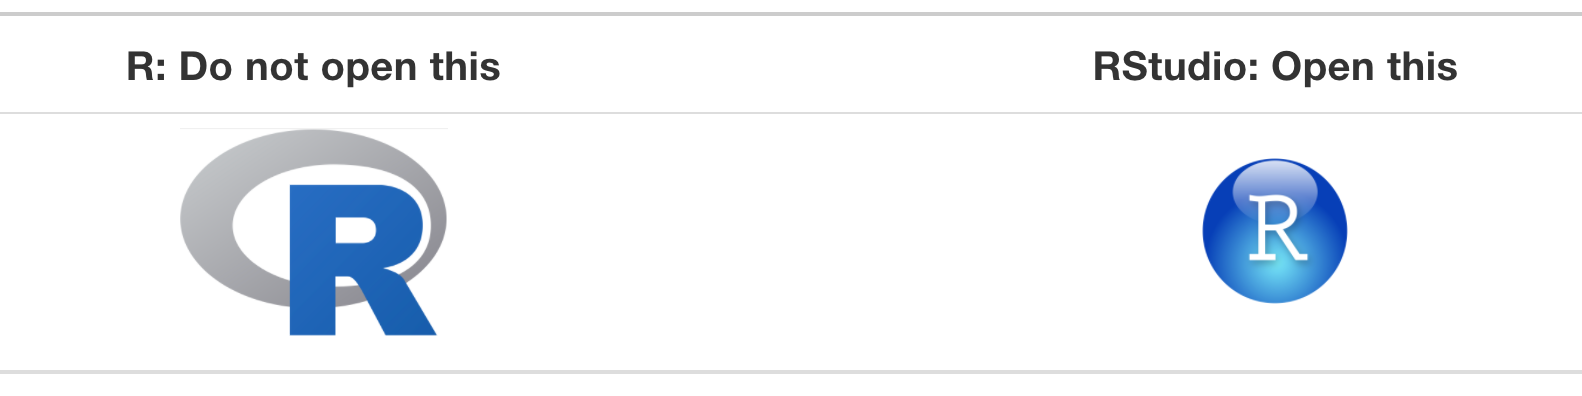
\includegraphics[width=0.9\linewidth]{images/logos/R_vs_RStudio} 

}

\caption{Icons of R versus RStudio on your computer.}\label{fig:R-vs-RStudio-2}
\end{figure}

After you open RStudio, you should see something similar to Figure \ref{fig:RStudio-interface}. (Note that slight differences might exist if the RStudio interface is updated to not be this by default.)

\begin{figure}[H]

{\centering 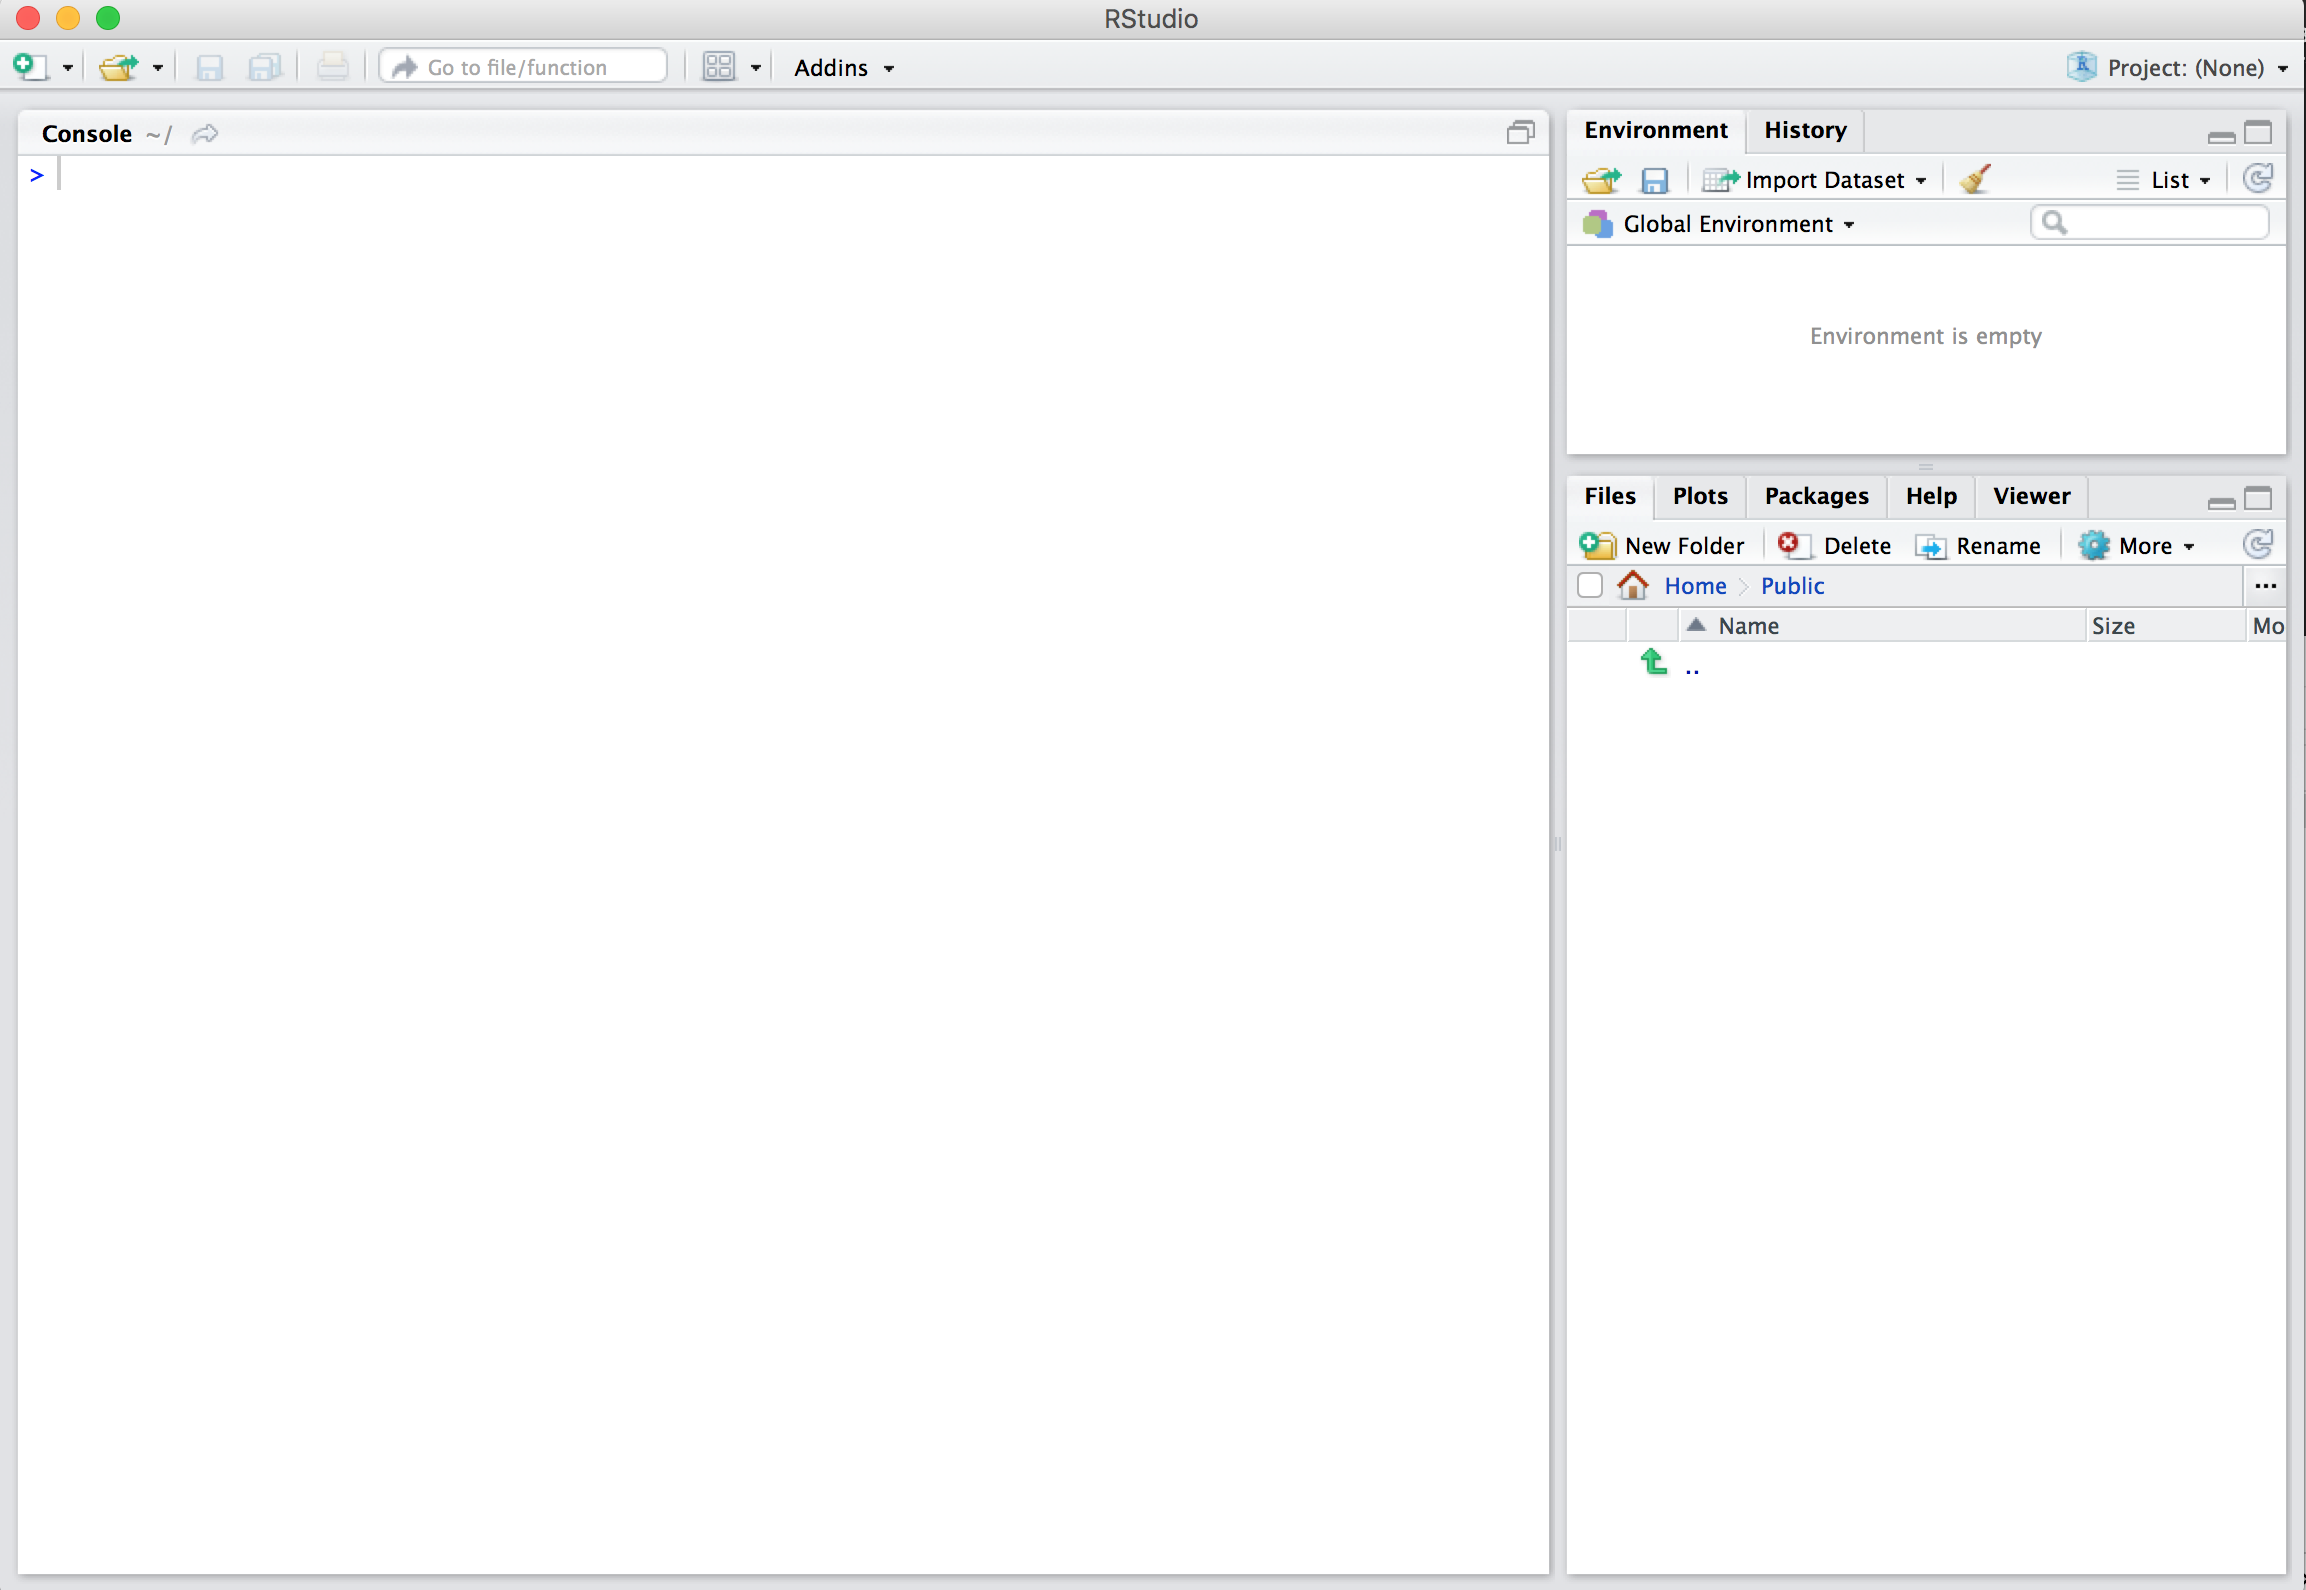
\includegraphics[width=0.93\linewidth]{images/rstudio_screenshots/rstudio} 

}

\caption{RStudio interface to R.}\label{fig:RStudio-interface}
\end{figure}

Note the three \emph{panes} which are three panels dividing the screen: the \emph{console pane}, the \emph{files pane}, and the \emph{environment pane}. Over the course of this chapter, you'll come to learn what purpose each of these panes serves.

\section{How do I code in R?}\label{code}

Now that you're set up with R and RStudio, you are probably asking yourself, ``OK. Now how do I use R?''. The first thing to note is that unlike other statistical software programs like Excel, SPSS, or Minitab that provide \href{https://en.wikipedia.org/wiki/Point_and_click}{point-and-click} interfaces, R is an \href{https://en.wikipedia.org/wiki/Interpreted_language}{interpreted language}. This means you have to type in commands written in \emph{R code}. In other words, you have to code/program in R. Note that we'll use the terms ``coding'' and ``programming'' interchangeably in this book.

While it is not required to be a seasoned coder/computer programmer to use R, there is still a set of basic programming concepts that new R users need to understand. Consequently, while this book is not a book on programming, you will still learn just enough of these basic programming concepts needed to explore and analyze data effectively.

\subsection{Basic programming concepts and terminology}\label{programming-concepts}

We now introduce some basic programming concepts and terminology. Instead of asking you to memorize all these concepts and terminology right now, we'll guide you so that you'll ``learn by doing.'' To help you learn, we will always use a different font to distinguish regular text from \texttt{computer\_code}. The best way to master these topics is, in our opinions, through \href{https://jamesclear.com/deliberate-practice-theory}{deliberate practice} with R and lots of repetition.

\begin{itemize}
\tightlist
\item
  Basics: \index{programming language basics}

  \begin{itemize}
  \tightlist
  \item
    \emph{Console pane}: where you enter in commands. \index{console}
  \item
    \emph{Running code}: the act of telling R to perform an act by giving it commands in the console.
  \item
    \emph{Objects}: where values are saved in R. We'll show you how to \emph{assign} values to objects and how to display the contents of objects. \index{objects}
  \item
    \emph{Data types}: integers, doubles/numerics, logicals, and characters. \index{data types} Integers are values like -1, 0, 2, 4092. Doubles or numerics are a larger set of values containing both the integers but also fractions and decimal values like -24.932 and 0.8. Logicals are either \texttt{TRUE} or \texttt{FALSE} while characters are text such as ``cabbage'', ``Hamilton'', ``The Wire is the greatest TV show ever'', and ``This ramen is delicious.'' Note that characters are often denoted with the quotation marks around them.
  \end{itemize}
\item
  \emph{Vectors}: a series of values. These are created using the \texttt{c()} function, where \texttt{c()} stands for ``combine'' or ``concatenate.'' For example, \texttt{c(6,\ 11,\ 13,\ 31,\ 90,\ 92)} creates a six element series of positive integer values \index{vectors}.
\item
  \emph{Factors}: \emph{categorical data} are commonly represented in R as factors. \index{factors} Categorical data can also be represented as \emph{strings}. We'll study this difference as we progress through the book.
\item
  \emph{Data frames}: rectangular spreadsheets. They are representations of datasets in R where the rows correspond to \emph{observations} and the columns correspond to \emph{variables} that describe the observations. \index{data frame} We'll cover data frames later in Section \ref{nycflights}.
\item
  \emph{Conditionals}: \index{conditionals}

  \begin{itemize}
  \tightlist
  \item
    Testing for equality in R using \texttt{==} (and not \texttt{=}, which is typically used for assignment). For example, \texttt{2\ +\ 1\ ==\ 3} compares \texttt{2\ +\ 1} to \texttt{3} and is correct R code, while \texttt{2\ +\ 1\ =\ 3} will return an error.
  \item
    Boolean algebra: \texttt{TRUE/FALSE} statements and mathematical operators such as \texttt{\textless{}} (less than), \texttt{\textless{}=} (less than or equal), and \texttt{!=} (not equal to). \index{Boolean algebra} For example, \texttt{4\ +\ 2\ \textgreater{}=\ 3} will return \texttt{TRUE}, but \texttt{3\ +\ 5\ \textless{}=\ 1} will return \texttt{FALSE}.
  \item
    Logical operators: \texttt{\&} representing ``and'' as well as \texttt{\textbar{}} representing ``or.'' For example, \texttt{(2\ +\ 1\ ==\ 3)\ \&\ (2\ +\ 1\ ==\ 4)} returns \texttt{FALSE} since both clauses are not \texttt{TRUE} (only the first clause is \texttt{TRUE}). On the other hand, \texttt{(2\ +\ 1\ ==\ 3)\ \textbar{}\ (2\ +\ 1\ ==\ 4)} returns \texttt{TRUE} since at least one of the two clauses is \texttt{TRUE}. \index{operators!logical}
  \end{itemize}
\item
  \emph{Functions}, also called \emph{commands}: Functions perform tasks in R. They take in inputs called \emph{arguments} and return outputs. You can either manually specify a function's arguments or use the function's \emph{default values}. \index{functions}

  \begin{itemize}
  \tightlist
  \item
    For example, the function \texttt{seq()} in R generates a sequence of numbers. If you just run \texttt{seq()} it will return the value 1. That doesn't seem very useful! This is because the default arguments are set as \texttt{seq(from\ =\ 1,\ to\ =\ 1)}. Thus, if you don't pass in different values for \texttt{from} and \texttt{to} to change this behavior, R just assumes all you want is the number 1. You can change the argument values by updating the values after the \texttt{=} sign. If we try out \texttt{seq(from\ =\ 2,\ to\ =\ 5)} we get the result \texttt{2\ 3\ 4\ 5} that we might expect.
  \item
    We'll work with functions a lot throughout this book and you'll get lots of practice in understanding their behaviors. To further assist you in understanding when a function is mentioned in the book, we'll also include the \texttt{()} after them as we did with \texttt{seq()} above.
  \end{itemize}
\end{itemize}

This list is by no means an exhaustive list of all the programming concepts and terminology needed to become a savvy R user; such a list would be so large it wouldn't be very useful, especially for novices. Rather, we feel this is a minimally viable list of programming concepts and terminology you need to know before getting started. We feel that you can learn the rest as you go. Remember that your mastery of all of these concepts and terminology will build as you practice more and more.

\subsection{Errors, warnings, and messages}\label{messages}

One thing that intimidates new R and RStudio users is how it reports \emph{errors}, \emph{warnings}, and \emph{messages}. R reports errors, warnings, and messages in a glaring red font, which makes it seem like it is scolding you. However, seeing red text in the console is not always bad.

R will show red text in the console pane in three different situations:

\begin{itemize}
\tightlist
\item
  \textbf{Errors}: \index{R!errors} When the red text is a legitimate error, it will be prefaced with ``Error in\ldots{}'' and will try to explain what went wrong. Generally when there's an error, the code will not run. For example, we'll see in Subsection \ref{package-use} if you see \texttt{Error\ in\ ggplot(...)\ :\ could\ not\ find\ function\ "ggplot"}, it means that the \texttt{ggplot()} function is not accessible because the package that contains the function (\texttt{ggplot2}) was not loaded with \texttt{library(ggplot2)}. Thus you cannot use the \texttt{ggplot()} function without the \texttt{ggplot2} package being loaded first.
\item
  \textbf{Warnings}: \index{R!warnings} When the red text is a warning, it will be prefaced with ``Warning:'' and R will try to explain why there's a warning. Generally your code will still work, but with some caveats. For example, you will see in Chapter \ref{viz} if you create a scatterplot based on a dataset where two of the rows of data have missing entries that would be needed to create points in the scatterplot, you will see this warning: \texttt{Warning:\ Removed\ 2\ rows\ containing\ missing\ values\ (geom\_point)}. R will still produce the scatterplot with all the remaining non-missing values, but it is warning you that two of the points aren't there.
\item
  \textbf{Messages}: \index{R!messages} When the red text doesn't start with either ``Error'' or ``Warning'', it's \emph{just a friendly message}. You'll see these messages when you load \emph{R packages} in the upcoming Subsection \ref{package-loading} or when you read data saved in spreadsheet files with the \texttt{read\_csv()} function as you'll see in Chapter \ref{tidy}. These are helpful diagnostic messages and they don't stop your code from working. Additionally, you'll see these messages when you install packages too using \texttt{install.packages()} as discussed in Subsection \ref{package-installation}.
\end{itemize}

Remember, when you see red text in the console, \emph{don't panic}. It doesn't necessarily mean anything is wrong. Rather:

\begin{itemize}
\tightlist
\item
  If the text starts with ``Error'', figure out what's causing it. {Think of errors as a red traffic light: something is wrong!}
\item
  If the text starts with ``Warning'', figure out if it's something to worry about. For instance, if you get a warning about missing values in a scatterplot and you know there are missing values, you're fine. If that's surprising, look at your data and see what's missing. {Think of warnings as a yellow traffic light: everything is working fine, but watch out/pay attention.}
\item
  Otherwise, the text is just a message. Read it, wave back at R, and thank it for talking to you. {Think of messages as a green traffic light: everything is working fine and keep on going!}
\end{itemize}

\subsection{Tips on learning to code}\label{tips-code}

Learning to code/program is quite similar to learning a foreign language. It can be daunting and frustrating at first. Such frustrations are common and it is normal to feel discouraged as you learn. However, just as with learning a foreign language, if you put in the effort and are not afraid to make mistakes, anybody can learn and improve.

Here are a few useful tips to keep in mind as you learn to program:

\begin{itemize}
\tightlist
\item
  \textbf{Remember that computers are not actually that smart}: You may think your computer or smartphone is ``smart,'' but really people spent a lot of time and energy designing them to appear ``smart.'' In reality, you have to tell a computer everything it needs to do. Furthermore, the instructions you give your computer can't have any mistakes in them, nor can they be ambiguous in any way.
\item
  \textbf{Take the ``copy, paste, and tweak'' approach}: Especially when you learn your first programming language or you need to understand particularly complicated code, it is often much easier to take existing code that you know works and modify it to suit your ends. This is as opposed to trying to type out the code from scratch. We call this the \emph{``copy, paste, and tweak''} approach. So early on, we suggest not trying to write code from memory, but rather take existing examples we have provided you, then copy, paste, and tweak them to suit your goals. After you start feeling more confident, you can slowly move away from this approach and write code from scratch. Think of the ``copy, paste, and tweak'' approach as training wheels for a child learning to ride a bike. After getting comfortable, they won't need them anymore.
\item
  \textbf{The best way to learn to code is by doing}: Rather than learning to code for its own sake, we find that learning to code goes much smoother when you have a goal in mind or when you are working on a particular project, like analyzing data that you are interested in and that is important to you.
\item
  \textbf{Practice is key}: Just as the only method to improve your foreign language skills is through lots of practice and speaking, the only method to improving your coding skills is through lots of practice. Don't worry, however, we'll give you plenty of opportunities to do so!
\end{itemize}

\section{What are R packages?}\label{packages}

Another point of confusion with many new R users is the idea of an R package. R packages \index{R!packages} extend the functionality of R by providing additional functions, data, and documentation. They are written by a worldwide community of R users and can be downloaded for free from the internet.

For example, among the many packages we will use in this book are the \texttt{ggplot2} package \citep{R-ggplot2} for data visualization in Chapter \ref{viz}\index{R packages!ggplot2}, the \texttt{dplyr} package \citep{R-dplyr} for data wrangling in Chapter \ref{wrangling}\index{R packages!dplyr}, the \texttt{moderndive} package \citep{R-moderndive} that accompanies this book\index{R packages!moderndive}, and the \texttt{infer} package \citep{R-infer} for ``tidy'' and transparent statistical inference in Chapters \ref{confidence-intervals}, \ref{hypothesis-testing}, and \ref{inference-for-regression}\index{R packages!infer}.

A good analogy for R packages \index{R packages} is they are like apps you can download onto a mobile phone:

\begin{figure}[H]

{\centering 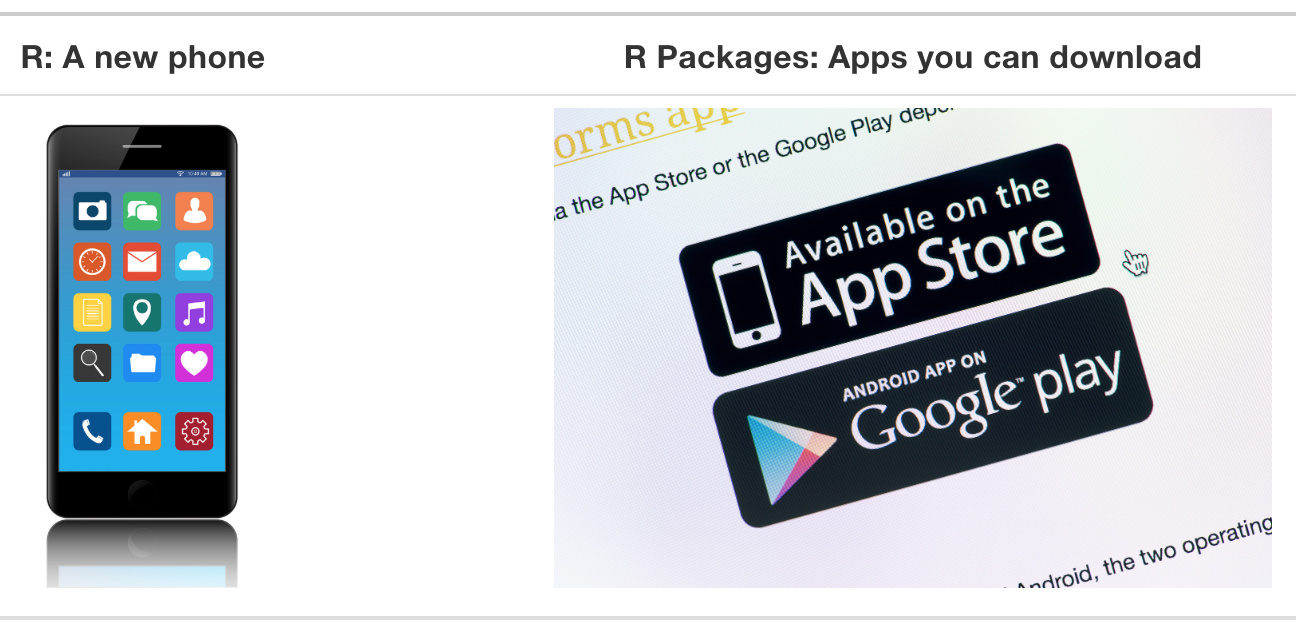
\includegraphics[width=0.7\linewidth]{images/shutterstock/R_vs_R_packages} 

}

\caption{Analogy of R versus R packages.}\label{fig:R-vs-R-packages}
\end{figure}

So R is like a new mobile phone: while it has a certain amount of features when you use it for the first time, it doesn't have everything. R packages are like the apps you can download onto your phone from Apple's App Store or Android's Google Play.

Let's continue this analogy by considering the Instagram app for editing and sharing pictures. Say you have purchased a new phone and you would like to share a photo you have just taken with friends on Instagram. You need to:

\begin{enumerate}
\def\labelenumi{\arabic{enumi}.}
\tightlist
\item
  \emph{Install the app}: Since your phone is new and does not include the Instagram app, you need to download the app from either the App Store or Google Play. You do this once and you're set for the time being. You might need to do this again in the future when there is an update to the app.
\item
  \emph{Open the app}: After you've installed Instagram, you need to open it.
\end{enumerate}

Once Instagram is open on your phone, you can then proceed to share your photo with your friends and family. The process is very similar for using an R package. You need to:

\begin{enumerate}
\def\labelenumi{\arabic{enumi}.}
\tightlist
\item
  \emph{Install the package}: This is like installing an app on your phone. Most packages are not installed by default when you install R and RStudio. Thus if you want to use a package for the first time, you need to install it first. Once you've installed a package, you likely won't install it again unless you want to update it to a newer version.
\item
  \emph{``Load'' the package}: ``Loading'' a package is like opening an app on your phone. Packages are not ``loaded'' by default when you start RStudio on your computer; you need to ``load'' each package you want to use every time you start RStudio.
\end{enumerate}

Let's perform these two steps for the \texttt{ggplot2} package for data visualization.

\subsection{Package installation}\label{package-installation}

\begin{quote}
\textbf{Note about RStudio Server or RStudio Cloud}: If your instructor has provided you with a link and access to RStudio Server or RStudio Cloud, you might not need to install packages, as they might be preinstalled for you by your instructor. That being said, it is still a good idea to know this process for later on when you are not using RStudio Server or Cloud, but rather RStudio Desktop on your own computer.
\end{quote}

There are two ways to install an R package: an easy way and a more advanced way. \index{R packages!installation} Let's install the \texttt{ggplot2} package the easy way first as shown in Figure \ref{fig:easy-way-install}. In the Files pane of RStudio:

\begin{enumerate}
\def\labelenumi{\alph{enumi})}
\tightlist
\item
  Click on the ``Packages'' tab.
\item
  Click on ``Install'' next to Update.
\item
  Type the name of the package under ``Packages (separate multiple with space or comma):'' In this case, type \texttt{ggplot2}.
\item
  Click ``Install.''
\end{enumerate}

\begin{figure}[H]

{\centering 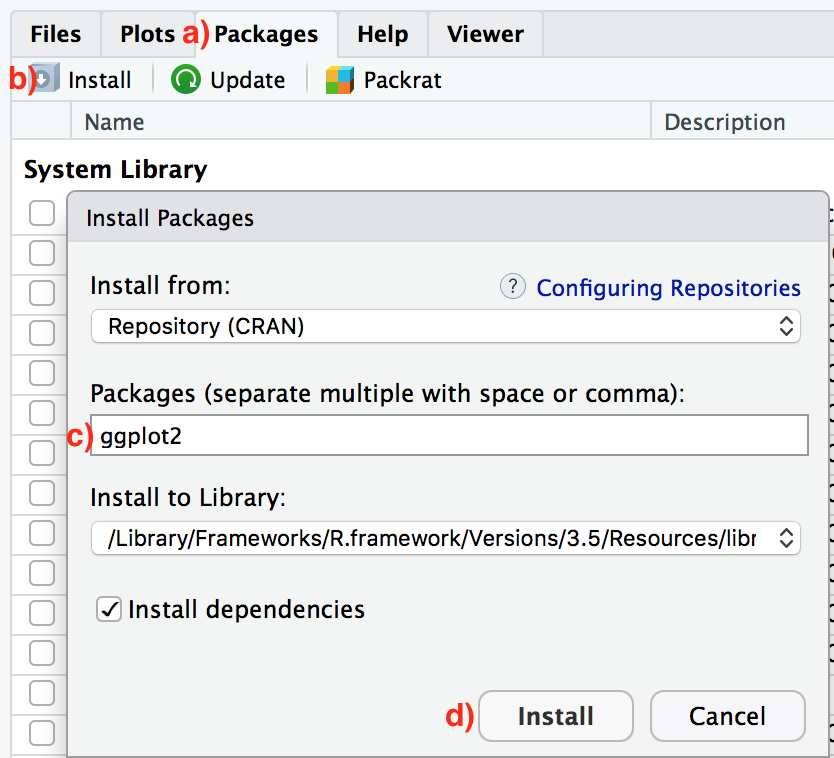
\includegraphics[width=0.49\linewidth,height=0.49\textheight]{images/rstudio_screenshots/install_packages_easy_way} 

}

\caption{Installing packages in R the easy way.}\label{fig:easy-way-install}
\end{figure}

An alternative but slightly less convenient way to install a package is by typing \texttt{install.packages("ggplot2")} in the console pane of RStudio and pressing Return/Enter on your keyboard. Note you must include the quotation marks around the name of the package.

Much like an app on your phone, you only have to install a package once. However, if you want to update a previously installed package to a newer version, you need to re-install it by repeating the earlier steps.

\vspace{0.1in}

\begin{learncheck}
\vspace{-0.15in}

\textbf{\emph{Learning check}} \vspace{-0.1in}
\end{learncheck}

\textbf{(LC1.1)} Repeat the earlier installation steps, but for the \texttt{dplyr}, \texttt{nycflights23}, and \texttt{knitr} packages. This will install the earlier mentioned \texttt{dplyr} package for data wrangling, the \texttt{nycflights23} package containing data on all domestic flights leaving a NYC airport in 2023, and the \texttt{knitr} package for generating easy-to-read tables in R. We'll use these packages in the next section.

\begin{learncheck}
\vspace{-0.25in}
\vspace{-0.25in}
\end{learncheck}

\subsection{Package loading}\label{package-loading}

Recall that after you've installed a package, you need to ``load it.'' In other words, you need to ``open it.'' We do this by using the \texttt{library()} command. \index{R packages!loading}

For example, to load the \texttt{ggplot2} package, run the following code in the console pane. What do we mean by ``run the following code''? Either type or copy-and-paste the following code into the console pane and then hit the Enter key.

\begin{Shaded}
\begin{Highlighting}[]
\FunctionTok{library}\NormalTok{(ggplot2)}
\end{Highlighting}
\end{Shaded}

If after running the earlier code, a blinking cursor returns next to the \texttt{\textgreater{}} ``prompt'' sign, it means you were successful and the \texttt{ggplot2} package is now loaded and ready to use. If, however, you get a red ``error message'' that reads \texttt{...} \index{R packages!loading error}

\begin{verbatim}
Error in library(ggplot2) : there is no package called ‘ggplot2’
\end{verbatim}

\texttt{...} it means that you didn't successfully install it. This is an example of an ``error message'' we discussed in Subsection \ref{messages}. If you get this error message, go back to Subsection \ref{package-installation} on R package installation and make sure to install the \texttt{ggplot2} package before proceeding.

\vspace{0.1in}

\begin{learncheck}
\vspace{-0.15in}

\textbf{\emph{Learning check}} \vspace{-0.1in}
\end{learncheck}

\textbf{(LC1.2)} ``Load'' the \texttt{dplyr}, \texttt{nycflights23}, and \texttt{knitr} packages as well by repeating the earlier steps.

\begin{learncheck}
\vspace{-0.25in}
\vspace{-0.25in}
\end{learncheck}

\vspace{0.1in}

\subsection{Package use}\label{package-use}

One very common mistake new R users make when wanting to use particular packages is they forget to ``load'' them first by using the \texttt{library()} command we just saw. Remember: \emph{you have to load each package you want to use every time you start RStudio.} If you don't first ``load'' a package, but attempt to use one of its features, you'll see an error message similar to:

\begin{verbatim}
Error: could not find function
\end{verbatim}

This is a different error message than the one you just saw on a package not having been installed yet. R is telling you that you are trying to use a function in a package that has not yet been ``loaded.'' R doesn't know where to find the function you are using. Almost all new users forget to do this when starting out, and it is a little annoying to get used to doing it. However, you'll remember with practice and after some time it will become second nature for you.

\section{Explore your first datasets}\label{nycflights}

Let's put everything we've learned so far into practice and start exploring some real data! Data comes to us in a variety of formats, from pictures to text to numbers. Throughout this book, we'll focus on datasets that are saved in ``spreadsheet''-type format. This is probably the most common way data are collected and saved in many fields. Remember from Subsection \ref{programming-concepts} that these ``spreadsheet''-type datasets are called \emph{data frames} in R. \index{data frame} We'll focus on working with data saved as data frames throughout this book.

Let's first load all the packages needed for this chapter, assuming you've already installed them. Read Section \ref{packages} for information on how to install and load R packages if you haven't already.

\begin{Shaded}
\begin{Highlighting}[]
\FunctionTok{library}\NormalTok{(nycflights23)}
\FunctionTok{library}\NormalTok{(dplyr)}
\FunctionTok{library}\NormalTok{(knitr)}
\end{Highlighting}
\end{Shaded}

At the beginning of all subsequent chapters in this book, we'll always have a list of packages that you should have installed and loaded in order to work with that chapter's R code.

\subsection{\texorpdfstring{\texttt{nycflights23} package}{nycflights23 package}}\label{nycflights23-package}

Many of us have flown on airplanes or know someone who has. Air travel has become an ever-present aspect of many people's lives. If you look at the Departures flight information board at an airport, you will frequently see that some flights are delayed for a variety of reasons. Are there ways that we can understand the reasons that cause flight delays?

We'd all like to arrive at our destinations on time whenever possible. (Unless you secretly love hanging out at airports. If you are one of these people, pretend for a moment that you are very much anticipating being at your final destination.) Throughout this book, we're going to analyze data related to all domestic flights departing from one of New York City's three main airports in 2023: Newark Liberty International (EWR), John F. Kennedy International (JFK), and LaGuardia Airport (LGA). We'll access this data using the \texttt{nycflights23} \index{R packages!nycflights23} R package, which contains five datasets saved in five data frames:

\begin{itemize}
\tightlist
\item
  \texttt{flights}: Information on all flights.
\item
  \texttt{airlines}: A table matching airline names and their two-letter International Air Transport Association (IATA) airline codes (also known as carrier codes) for 14 airline companies. For example, ``DL'' is the two-letter code for Delta.
\item
  \texttt{planes}: Information about each of the 4,840 physical aircraft used.
\item
  \texttt{weather}: Hourly meteorological data for each of the three NYC airports. This data frame has 26,204 rows, roughly corresponding to the \(365 \times 24 \times 3 = 26,280\) possible hourly measurements one can observe at three locations over the course of a year.
\item
  \texttt{airports}: Names, codes, and locations of the 1,251 domestic destinations.
\end{itemize}

The \texttt{nycflights23} package is an updated version of \href{https://nycflights13.tidyverse.org/}{the classic \texttt{nycflights13} R package}. \texttt{nycflights23} was authored by ModernDive co-author Chester Ismay using the \href{https://anyflights.netlify.app/}{\texttt{anyflights} R package} developed by \href{https://www.simonpcouch.com/}{Simon Couch}. Simon granted permission to the ModernDive team to create \texttt{nycflights23} and submit the package to CRAN.

\subsection{\texorpdfstring{\texttt{flights} data frame}{flights data frame}}\label{flights-data-frame}

We'll begin by exploring the \texttt{flights} data frame and get an idea of its structure. Run the following code in your console, either by typing it or by cutting-and-pasting it. It displays the contents of the \texttt{flights} data frame in your console. Note that depending on the size of your monitor, the output may vary slightly.

\begin{Shaded}
\begin{Highlighting}[]
\NormalTok{flights}
\end{Highlighting}
\end{Shaded}

\begin{verbatim}
# A tibble: 435,352 x 19
    year month   day dep_time sched_dep_time dep_delay arr_time
   <int> <int> <int>    <int>          <int>     <dbl>    <int>
 1  2023     1     1        1           2038       203      328
 2  2023     1     1       18           2300        78      228
 3  2023     1     1       31           2344        47      500
 4  2023     1     1       33           2140       173      238
 5  2023     1     1       36           2048       228      223
 6  2023     1     1      503            500         3      808
 7  2023     1     1      520            510        10      948
 8  2023     1     1      524            530        -6      645
 9  2023     1     1      537            520        17      926
10  2023     1     1      547            545         2      845
# i 435,342 more rows
# i 12 more variables: sched_arr_time <int>, arr_delay <dbl>,
#   carrier <chr>, flight <int>, tailnum <chr>, origin <chr>, dest <chr>,
#   air_time <dbl>, distance <dbl>, hour <dbl>, minute <dbl>,
#   time_hour <dttm>
\end{verbatim}

Let's unpack this output:

\begin{itemize}
\tightlist
\item
  \texttt{A\ tibble:\ 435,352\ x\ 19}: A \texttt{tibble} is a specific kind of data frame in R.\index{tibble} This particular data frame has

  \begin{itemize}
  \tightlist
  \item
    \texttt{435,352} rows corresponding to different \emph{observations}. Here, each observation is a flight.
  \item
    \texttt{19} columns corresponding to 19 \emph{variables} describing each observation.
  \end{itemize}
\item
  \texttt{year}, \texttt{month}, \texttt{day}, \texttt{dep\_time}, \texttt{sched\_dep\_time}, \texttt{dep\_delay}, and \texttt{arr\_time} are the different columns, in other words, the different variables of this dataset.
\item
  We then have a preview of the first 10 rows of observations corresponding to the first 10 flights. R is only showing the first 10 rows, because if it showed all \texttt{435,352} rows, it would overwhelm your screen.
\item
  \texttt{...\ with\ 435,342\ more\ rows\textasciigrave{}\ and\ 11\ more\ variables:} indicating to us that 435,342 more rows of data and 11 more variables could not fit in this screen.
\end{itemize}

Unfortunately, this output does not allow us to explore the data very well, but it does give a nice preview. Let's look at some different ways to explore data frames.

\subsection{Exploring data frames}\label{exploredataframes}

There are many ways to get a feel for the data contained in a data frame such as \texttt{flights}. We present three functions that take as their ``argument'' (their input) a data frame and a fourth method for exploring one column of a data frame:

\begin{enumerate}
\def\labelenumi{\arabic{enumi}.}
\tightlist
\item
  Using the \texttt{View()} function, which brings up RStudio's built-in data viewer.
\item
  Using the \texttt{glimpse()} function, which is included in the \texttt{dplyr} package.
\item
  Using the \texttt{kable()} function, which is included in the \texttt{knitr} package.
\item
  Using the \texttt{\$} ``extraction operator,'' which is used to view a single variable.
\end{enumerate}

\textbf{1. \texttt{View()}}:

Run \texttt{View(flights)} \index{R packages!utils!View()} in your console in RStudio, either by typing it or cutting-and-pasting it into the console pane. Explore this data frame in the resulting pop up viewer. You should get into the habit of viewing any data frames you encounter. Note the uppercase \texttt{V} in \texttt{View()}. R is case-sensitive, so you'll get an error message if you run \texttt{view(flights)} instead of \texttt{View(flights)}.

\vspace{0.1in}

\begin{learncheck}
\vspace{-0.15in}

\textbf{\emph{Learning check}} \vspace{-0.1in}
\end{learncheck}

\textbf{(LC1.3)} What does any \emph{ONE} row in this \texttt{flights} dataset refer to?

\begin{itemize}
\tightlist
\item
  A. Data on an airline
\item
  B. Data on a flight
\item
  C. Data on an airport
\item
  D. Data on multiple flights
\end{itemize}

\begin{learncheck}
\vspace{-0.25in}
\vspace{-0.25in}
\end{learncheck}

\vspace{0.1in}

By running \texttt{View(flights)}, we can explore the different \emph{variables} listed in the columns. Observe that there are many different types of variables. Some of the variables like \texttt{distance}, \texttt{day}, and \texttt{arr\_delay} are what we will call \emph{quantitative} variables. \index{quantitative} These variables are numerical in nature. Other variables here are \index{categorical} \emph{categorical}.

If you look in the leftmost column of the \texttt{View(flights)} output, you'll see a column of numbers. These are the row numbers of the dataset. Glancing across a row with the same number, say row 5, you can get an idea of what each row represents. This allows you to identify what object is being described in a given row by taking note of the values of the columns in that specific row. This is often called the \emph{observational unit}.\index{observational unit} The observational unit in this example is an individual flight departing from New York City in 2023. You can identify the observational unit by determining what ``thing'' is being measured or described by each of the variables. We'll talk more about observational units in Subsection \ref{identification-vs-measurement-variables} on \emph{identification} and \emph{measurement} variables.

\textbf{2. \texttt{glimpse()}}:

The second way we'll cover to explore a data frame is using the \texttt{glimpse()} function \index{R packages!dplyr!glimpse()} included in the \index{R packages!dplyr} \texttt{dplyr} package. Thus, you can only use the \texttt{glimpse()} function after you've loaded the \texttt{dplyr} package by running \texttt{library(dplyr)}. This function provides us with an alternative perspective for exploring a data frame than the \texttt{View()} function:

\begin{Shaded}
\begin{Highlighting}[]
\FunctionTok{glimpse}\NormalTok{(flights)}
\end{Highlighting}
\end{Shaded}

\begin{verbatim}
Rows: 435,352
Columns: 19
$ year           <int> 2023, 2023, 2023, 2023, 2023, 2023, 2023, 2023, 20~
$ month          <int> 1, 1, 1, 1, 1, 1, 1, 1, 1, 1, 1, 1, 1, 1, 1, 1, 1,~
$ day            <int> 1, 1, 1, 1, 1, 1, 1, 1, 1, 1, 1, 1, 1, 1, 1, 1, 1,~
$ dep_time       <int> 1, 18, 31, 33, 36, 503, 520, 524, 537, 547, 549, 5~
$ sched_dep_time <int> 2038, 2300, 2344, 2140, 2048, 500, 510, 530, 520, ~
$ dep_delay      <dbl> 203, 78, 47, 173, 228, 3, 10, -6, 17, 2, -10, -9, ~
$ arr_time       <int> 328, 228, 500, 238, 223, 808, 948, 645, 926, 845, ~
$ sched_arr_time <int> 3, 135, 426, 2352, 2252, 815, 949, 710, 818, 852, ~
$ arr_delay      <dbl> 205, 53, 34, 166, 211, -7, -1, -25, 68, -7, 4, -13~
$ carrier        <chr> "UA", "DL", "B6", "B6", "UA", "AA", "B6", "AA", "U~
$ flight         <int> 628, 393, 371, 1053, 219, 499, 996, 981, 206, 225,~
$ tailnum        <chr> "N25201", "N830DN", "N807JB", "N265JB", "N17730", ~
$ origin         <chr> "EWR", "JFK", "JFK", "JFK", "EWR", "EWR", "JFK", "~
$ dest           <chr> "SMF", "ATL", "BQN", "CHS", "DTW", "MIA", "BQN", "~
$ air_time       <dbl> 367, 108, 190, 108, 80, 154, 192, 119, 258, 157, 1~
$ distance       <dbl> 2500, 760, 1576, 636, 488, 1085, 1576, 719, 1400, ~
$ hour           <dbl> 20, 23, 23, 21, 20, 5, 5, 5, 5, 5, 5, 6, 5, 6, 6, ~
$ minute         <dbl> 38, 0, 44, 40, 48, 0, 10, 30, 20, 45, 59, 0, 59, 0~
$ time_hour      <dttm> 2023-01-01 20:00:00, 2023-01-01 23:00:00, 2023-01~
\end{verbatim}

Observe that \texttt{glimpse()} will give you the first few entries of each variable in a row after the variable name. In addition, the \emph{data type} (see Subsection \ref{programming-concepts}) of the variable is given immediately after each variable's name inside \texttt{\textless{}\ \textgreater{}}. Here, \texttt{int} and \texttt{dbl} refer to ``integer'' and ``double'', which are computer coding terminology for quantitative/numerical variables. ``Doubles'' take up twice the size to store on a computer compared to integers.

In contrast, \texttt{chr} refers to ``character'', which is computer terminology for text data. In most forms, text data, such as the \texttt{carrier} or \texttt{origin} of a flight, are categorical variables. The \texttt{time\_hour} variable is another data type: \texttt{dttm}. These types of variables represent date and time combinations. However, we won't work with dates and times in this book; we leave this topic for other data science books like \href{https://datasciencebook.ca/}{\emph{Data Science: A First Introduction} by Tiffany-Anne Timbers, Melissa Lee, and Trevor Campbell} or \href{https://r4ds.had.co.nz/dates-and-times.html}{\emph{R for Data Science}} \citep{rds2016}.

\vspace*{0.05in}

\begin{learncheck}
\vspace{-0.15in}

\textbf{\emph{Learning check}} \vspace{-0.1in}
\end{learncheck}

\textbf{(LC1.4)} What are some other examples in this dataset of \emph{categorical} variables? What makes them different than \emph{quantitative} variables?

\begin{learncheck}
\vspace{-0.25in}
\vspace{-0.25in}
\end{learncheck}

\textbf{3. \texttt{kable()}}:

The final way to explore the entirety of a data frame is using the \texttt{kable()} \index{R packages!knitr!kable()} function from the \index{knitr|seealso{R packages!knitr}} \texttt{knitr} package. Let's explore the different carrier codes for all the airlines in our dataset two ways. Run both of these lines of code in the console:

\begin{Shaded}
\begin{Highlighting}[]
\NormalTok{airlines}
\FunctionTok{kable}\NormalTok{(airlines)}
\end{Highlighting}
\end{Shaded}

At first glance, it may not appear that there is much difference in the outputs. However, when using tools for producing reproducible reports such as \href{http://rmarkdown.rstudio.com/lesson-1.html}{R Markdown}, the latter code produces output that is much more legible and reader-friendly. You'll see us use this reader-friendly style in many places in the book when we want to print a data frame as a nice table.

\textbf{4. \texttt{\$} operator}

Lastly, the \texttt{\$} operator \index{operators!dollar sign} allows us to extract and then explore a single variable within a data frame. For example, run the following in your console:

\begin{Shaded}
\begin{Highlighting}[]
\NormalTok{airlines}\SpecialCharTok{$}\NormalTok{name}
\end{Highlighting}
\end{Shaded}

We used the \texttt{\$} operator to extract only the \texttt{name} variable and return it as a vector of length 16\index{vectors}. We'll only be occasionally exploring data frames using the \texttt{\$} operator, instead favoring the \texttt{View()} and \texttt{glimpse()} functions.

\subsection{Identification and measurement variables}\label{identification-vs-measurement-variables}

There is a subtle difference between the kinds of variables that you will encounter in data frames. There are \emph{identification variables} and \emph{measurement variables}. For example, let's explore the \texttt{airports} data frame by showing the output of \texttt{glimpse(airports)}:

\begin{Shaded}
\begin{Highlighting}[]
\FunctionTok{glimpse}\NormalTok{(airports)}
\end{Highlighting}
\end{Shaded}

\begin{verbatim}
Rows: 1,251
Columns: 8
$ faa   <chr> "AAF", "AAP", "ABE", "ABI", "ABL", "ABQ", "ABR", "ABY", "AC~
$ name  <chr> "Apalachicola Regional Airport", "Andrau Airpark", "Lehigh ~
$ lat   <dbl> 29.7, 29.7, 40.7, 32.4, 67.1, 35.0, 45.4, 31.5, 41.3, 31.6,~
$ lon   <dbl> -85.0, -95.6, -75.4, -99.7, -157.9, -106.6, -98.4, -84.2, -~
$ alt   <dbl> 20, 79, 393, 1791, 334, 5355, 1302, 197, 47, 516, 221, 75, ~
$ tz    <dbl> -5, -6, -5, -6, -9, -7, -6, -5, -5, -6, -8, -5, -10, -6, -9~
$ dst   <chr> "A", "A", "A", "A", "A", "A", "A", "A", "A", "A", "A", "A",~
$ tzone <chr> "America/New_York", "America/Chicago", "America/New_York", ~
\end{verbatim}

The variables \texttt{faa} and \texttt{name} are \emph{identification variables} that uniquely identify each airport. \texttt{faa} provides the airport's unique FAA code, while \texttt{name} gives its official name. These variables are used to uniquely identify each row in a data frame. The remaining variables (\texttt{lat}, \texttt{lon}, \texttt{alt}, \texttt{tz}, \texttt{dst}, \texttt{tzone}) are often called \emph{measurement} or \emph{characteristic} variables: variables that describe properties of each observational unit. For example, \texttt{lat} and \texttt{long} describe the latitude and longitude of each airport.

Furthermore, sometimes a single variable might not be enough to uniquely identify each observational unit: combinations of variables might be needed. While it is not an absolute rule, for organizational purposes it is considered good practice to have your identification variables in the leftmost columns of your data frame.

\begin{learncheck}
\vspace{-0.15in}

\textbf{\emph{Learning check}} \vspace{-0.1in}
\end{learncheck}

\textbf{(LC1.5)} What properties of each airport do the variables \texttt{lat}, \texttt{lon}, \texttt{alt}, \texttt{tz}, \texttt{dst}, and \texttt{tzone} describe in the \texttt{airports} data frame? Take your best guess.

\textbf{(LC1.6)} Provide the names of variables in a data frame with at least three variables where one of them is an identification variable and the other two are not.

\begin{learncheck}
\vspace{-0.25in}
\vspace{-0.25in}
\end{learncheck}

\subsection{Help files}\label{help-files}

Another nice feature of R are help files, which provide documentation for various functions and datasets. You can bring up help files by adding a \texttt{?} \index{operators!?} before the name of a function or data frame and then run this in the console. You will then be presented with a page showing the corresponding documentation if it exists. For example, let's look at the help file for the \texttt{flights} data frame.

\begin{Shaded}
\begin{Highlighting}[]
\NormalTok{?flights}
\end{Highlighting}
\end{Shaded}

The help file should pop up in the Help pane of RStudio. If you have questions about a function or data frame included in an R package, you should get in the habit of consulting the help file right away.

\begin{learncheck}
\vspace{-0.15in}

\textbf{\emph{Learning check}} \vspace{-0.1in}
\end{learncheck}

\textbf{(LC1.7)} Look at the help file for the \texttt{airports} data frame. Revise your earlier guesses about what the variables \texttt{lat}, \texttt{lon}, \texttt{alt}, \texttt{tz}, \texttt{dst}, and \texttt{tzone} each describe.

\begin{learncheck}
\vspace{-0.25in}
\vspace{-0.25in}
\end{learncheck}

\section{Conclusion}\label{conclusion}

We've given you what we feel is a minimally viable set of tools to explore data in R. Does this chapter contain everything you need to know? Absolutely not. To try to include everything in this chapter would make the chapter so large it wouldn't be useful! As we said earlier, the best way to add to your toolbox is to get into RStudio and run and write code as much as possible.

\subsection{Additional resources}\label{additional-resources}

Solutions to all \emph{Learning checks} can be found in the Appendices of the online version of the book. The Appendices start at \url{https://moderndive.com/v2/appendixa}.

If you are new to the world of coding, R, and RStudio and feel you could benefit from a more detailed introduction, we suggest you check out the short book, \href{https://rbasics.netlify.app/}{\emph{Getting Used to R, RStudio, and R Markdown}} \citep{usedtor2016}. It includes screencast recordings that you can follow along and pause as you learn. This book also contains an introduction to R Markdown, a tool used for reproducible research in R.



\begin{figure}[H]

{\centering 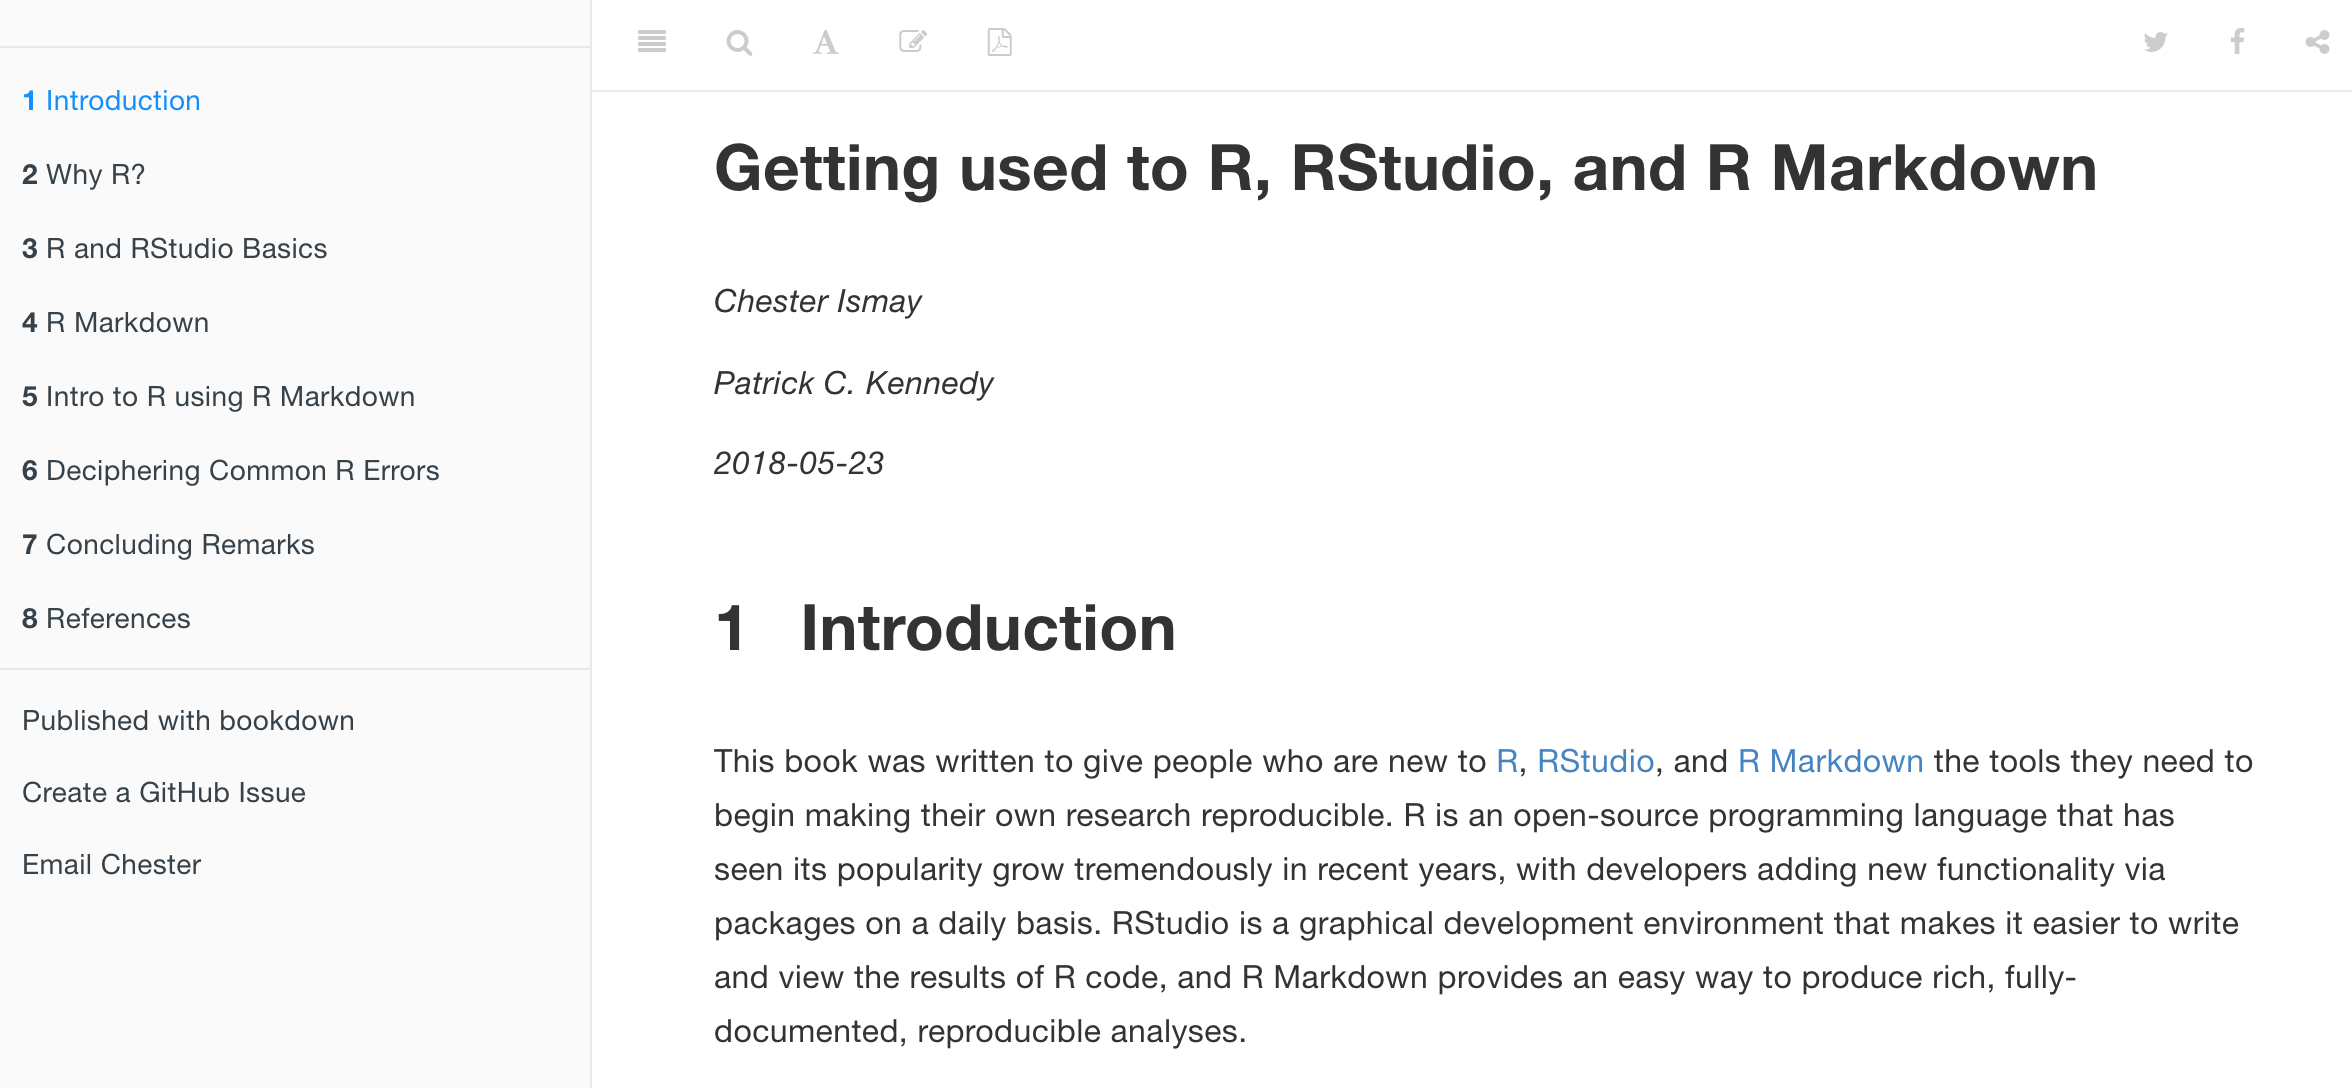
\includegraphics[width=\textwidth]{images/copyright/getting-used-to-R} 

}

\caption{Preview of \emph{Getting Used to R, RStudio, and R Markdown}.}\label{fig:unnamed-chunk-31}
\end{figure}

\subsection{What's to come?}\label{whats-to-come}

We're now going to start the ``Data Science with \texttt{tidyverse}'' portion of this book in Chapter \ref{viz} as shown in Figure \ref{fig:moderndive-flowchart} with what we feel is the most important tool in a data scientist's toolbox: data visualization. We'll continue to explore the data included in the \texttt{moderndive} and \texttt{nycflights23} packages using the \texttt{ggplot2} package for data visualization. You'll see that data visualization is a powerful tool to add to your toolbox for data exploration that provides additional insight to what the \texttt{View()} and \texttt{glimpse()} functions can provide.



\begin{figure}[H]

{\centering 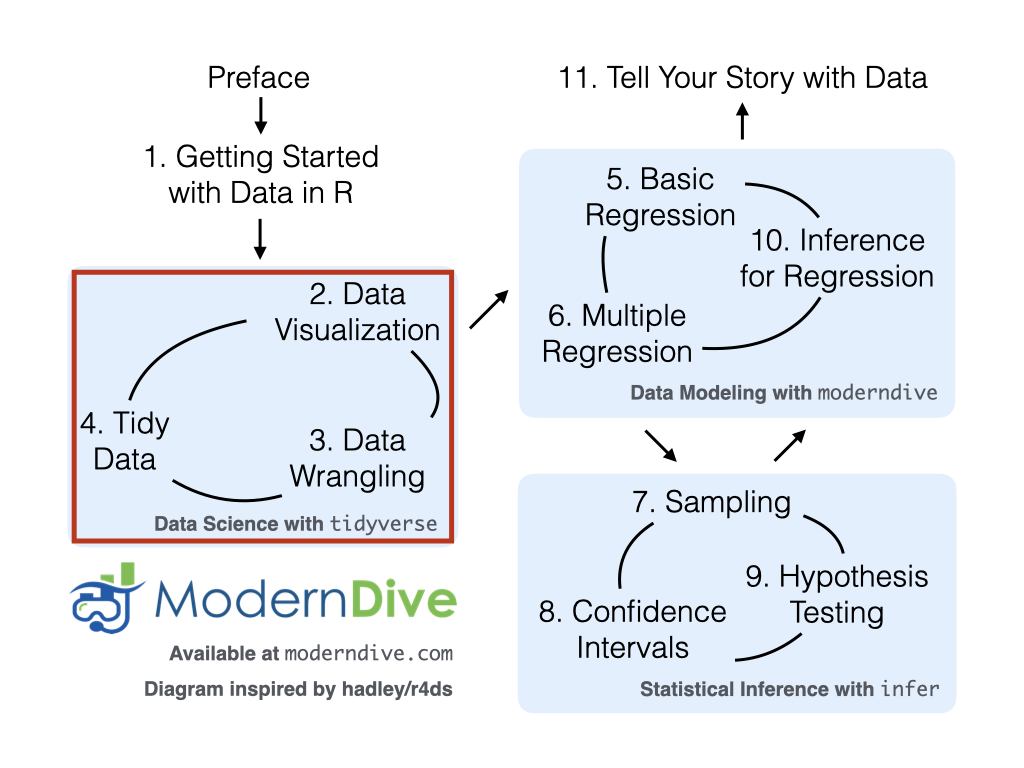
\includegraphics[width=0.6\linewidth,height=0.6\textheight]{images/flowcharts/flowchart/flowchart.004} 

}

\caption{\emph{ModernDive} flowchart - on to Part I!}\label{fig:moderndive-flowchart}
\end{figure}



\part{Data Science with \texttt{tidyverse}}\label{part-reftidyversepart}

\chapter{Data Visualization}\label{viz}

We begin the development of your data science toolbox with data visualization. By visualizing data, we gain valuable insights we couldn't initially obtain from just looking at the raw data values. We'll use the \texttt{ggplot2} package, as it provides an easy way to customize your plots. \texttt{ggplot2} is rooted in the data visualization theory known as \emph{the grammar of graphics} \citep{wilkinson2005}, developed by Leland Wilkinson. \index{Wilkinson, Leland}

At their most basic, graphics/plots/charts (we use these terms interchangeably in this book) provide a nice way to explore the patterns in data, such as the presence of \emph{outliers}, \emph{distributions} of individual variables, and \emph{relationships} between groups of variables. Graphics are designed to emphasize the findings and insights you want your audience to understand. This does, however, require a balancing act. On the one hand, you want to highlight as many interesting findings as possible. On the other hand, you don't want to include so much information that it overwhelms your audience.

As we will see, plots \index{plots} also help us to identify patterns and outliers in our data. We'll see that a common extension of these ideas is to compare the \emph{distribution} \index{distribution} of one numerical variable, such as what are the center and spread of the values, as we go across the levels of a different categorical variable.

\subsection*{Needed packages}\label{needed-packages}


Let's load all the packages needed for this chapter (this assumes you've already installed them). Read Section \ref{packages} for information on how to install and load R packages.

\begin{Shaded}
\begin{Highlighting}[]
\FunctionTok{library}\NormalTok{(nycflights23)}
\FunctionTok{library}\NormalTok{(ggplot2)}
\FunctionTok{library}\NormalTok{(moderndive)}
\FunctionTok{library}\NormalTok{(tibble)}
\end{Highlighting}
\end{Shaded}

\section{The grammar of graphics}\label{grammarofgraphics}

We start with a discussion of a theoretical framework for data visualization known as ``the grammar of graphics.'' This framework serves as the foundation for the \index{R packages!ggplot2} \texttt{ggplot2} package which we'll use extensively in this chapter. \index{Grammar of Graphics, The} Think of how we construct and form sentences in English by combining different elements, like nouns, verbs, articles, subjects, objects, etc. We can't just combine these elements in any arbitrary order; we must do so following a set of rules known as a linguistic grammar. Similarly to a linguistic grammar, ``the grammar of graphics'' defines a set of rules for constructing \emph{statistical graphics} by combining different types of \emph{layers}. This grammar was created by Leland Wilkinson \citep{wilkinson2005} and has been implemented in a variety of data visualization software platforms like R, but also \href{https://plot.ly/}{Plotly} and \href{https://www.tableau.com/}{Tableau}.

\subsection{Components of the grammar}\label{components-of-the-grammar}

In short, the grammar tells us that:

\begin{quote}
A statistical graphic is a \texttt{mapping} of \texttt{data} variables to \texttt{aes}thetic attributes of \texttt{geom}etric objects.
\end{quote}

Specifically, we can break a graphic into the following three essential components:

\begin{enumerate}
\def\labelenumi{\arabic{enumi}.}
\tightlist
\item
  \texttt{data}: the dataset containing the variables of interest.
\item
  \texttt{geom}: the geometric object in question. This refers to the type of object we can observe in a plot. For example: points, lines, and bars.
\item
  \texttt{aes}: aesthetic attributes of the geometric object. For example, x/y position, color, shape, and size. Aesthetic attributes are \emph{mapped} to variables in the dataset.
\end{enumerate}

You might be wondering why we wrote the terms \texttt{data}, \texttt{geom}, and \texttt{aes} in a computer code type font. We'll see very shortly that we'll specify the elements of the grammar in R using these terms. However, let's first break down the grammar with an example.

\subsection{Gapminder data}\label{gapminder}

In February 2006, a Swedish physician and data advocate named Hans Rosling gave a TED talk titled \href{https://www.ted.com/talks/hans_rosling_shows_the_best_stats_you_ve_ever_seen}{``The best stats you've ever seen''} where he presented global economic, health, and development data from the website \href{http://www.gapminder.org/tools/\#_locale_id=en;&chart-type=bubbles}{gapminder.org}. For example, for data on 142 countries in 2007, let's consider only a few countries in Table \ref{tab:gapminder-2007} as a peek into the data.

\begin{table}[H]
\centering
\caption{\label{tab:gapminder-2007}Gapminder 2007 Data: First 3 of 142 countries}
\centering
\fontsize{10}{12}\selectfont
\begin{tabular}[t]{l|l|r|r|r}
\hline
Country & Continent & Life Expectancy & Population & GDP per Capita\\
\hline
Afghanistan & Asia & 43.8 & 31889923 & 975\\
\hline
Albania & Europe & 76.4 & 3600523 & 5937\\
\hline
Algeria & Africa & 72.3 & 33333216 & 6223\\
\hline
\end{tabular}
\end{table}

Each row in this table corresponds to a country in 2007. For each row, we have 5 columns:

\begin{enumerate}
\def\labelenumi{\arabic{enumi}.}
\tightlist
\item
  \textbf{Country}: Name of country.
\item
  \textbf{Continent}: Which of the five continents the country is part of. Note that ``Americas'' includes countries in both North and South America and that Antarctica is excluded.
\item
  \textbf{Life Expectancy}: Life expectancy in years.
\item
  \textbf{Population}: Number of people living in the country.
\item
  \textbf{GDP per Capita}: Gross domestic product (in US dollars).
\end{enumerate}

Now consider Figure \ref{fig:gapminder}, which plots this for all 142 of the data's countries.

\begin{figure}[H]

{\centering 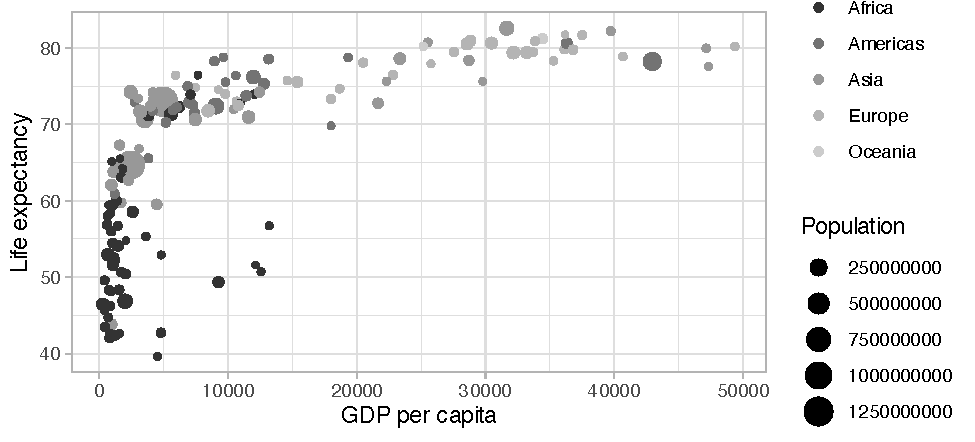
\includegraphics[width=\textwidth]{ModernDive_files/figure-latex/gapminder-1} 

}

\caption{Life expectancy over GDP per capita in 2007.}\label{fig:gapminder}
\end{figure}

Let's view this plot through the grammar of graphics:

\begin{enumerate}
\def\labelenumi{\arabic{enumi}.}
\tightlist
\item
  The \texttt{data} variable \textbf{GDP per Capita} gets mapped to the \texttt{x}-position \texttt{aes}thetic \index{R packages!ggplot2!aes()} of the points.
\item
  The \texttt{data} \index{R packages!ggplot2!data} variable \textbf{Life Expectancy} gets mapped to the \texttt{y}-position \texttt{aes}thetic of the points.
\item
  The \texttt{data} variable \textbf{Population} gets mapped to the \texttt{size} \texttt{aes}thetic of the points.
\item
  The \texttt{data} variable \textbf{Continent} gets mapped to the \texttt{color} \texttt{aes}thetic of the points.
\end{enumerate}

We'll see shortly that \texttt{data} corresponds to the particular data frame where our data is saved and that ``data variables'' correspond to particular columns in the data frame. Furthermore, the type of \texttt{geom}etric object \index{R packages!ggplot2!geom} considered in this plot are points. That being said, while in this example we are considering points, graphics are not limited to just points. We can also use lines, bars, and other geometric objects.

Let's summarize the three essential components of the grammar in Table \ref{tab:summary-table-gapminder}.

\begin{table}[H]
\centering
\caption{\label{tab:summary-table-gapminder}Summary of the grammar of graphics for this plot}
\centering
\fontsize{10}{12}\selectfont
\begin{tabular}[t]{lll}
\toprule
data variable & aes & geom\\
\midrule
GDP per Capita & x & point\\
Life Expectancy & y & point\\
Population & size & point\\
Continent & color & point\\
\bottomrule
\end{tabular}
\end{table}

\subsection{Other components}\label{other-components}

There are other components of the grammar of graphics we can control as well. As you start to delve deeper into the grammar of graphics, you'll start to encounter these topics more frequently. In this book, we'll keep things simple and only work with these two additional components:

\begin{itemize}
\tightlist
\item
  \texttt{facet}ing breaks up a plot into several plots split by the values of another variable (Section \ref{facets}) \index{R packages!ggplot2!facet}
\item
  \texttt{position} adjustments for barplots (Section \ref{geombar}) \index{R packages!ggplot2!position}
\end{itemize}

Other more complex components like \texttt{scales} and \texttt{coord}inate systems are left for a more advanced text such as \href{http://r4ds.had.co.nz/data-visualisation.html\#aesthetic-mappings}{\emph{R for Data Science}} \citep{rds2016}. Generally speaking, the grammar of graphics allows for a high degree of customization of plots and also a consistent framework for easily updating and modifying them.

\subsection{ggplot2 package}\label{ggplot2-package}

In this book, we will use the \texttt{ggplot2} package for data visualization, which is an implementation of the \textbf{g}rammar of \textbf{g}raphics for R \citep{R-ggplot2}. As we noted earlier, a lot of the previous section was written in a computer code type font. This is because the various components of the grammar of graphics are specified in the \texttt{ggplot()} \index{R packages!ggplot2!ggplot()} function included in the \texttt{ggplot2} package. For the purposes of this book, we'll always provide the \texttt{ggplot()} function with the following arguments (i.e., inputs) at a minimum:

\begin{itemize}
\tightlist
\item
  The data frame where the variables exist: the \texttt{data} argument.
\item
  The mapping of the variables to aesthetic attributes: the \texttt{mapping} argument which specifies the \texttt{aes}thetic attributes involved.
\end{itemize}

After we've specified these components, we then add \emph{layers} to the plot using the \texttt{+} sign. The most essential layer to add to a plot is the layer that specifies which type of \texttt{geom}etric object we want the plot to involve: points, lines, bars, and others. Other layers we can add to a plot include the plot title, axes labels, visual themes for the plots, and facets (which we'll see in Section \ref{facets}).

Let's now put the theory of the grammar of graphics into practice.

\section{Five named graphs - the 5NG}\label{FiveNG}

In order to keep things simple in this book, we will only focus on five different types of graphics, each with a commonly given name. We term these ``five named graphs'' or in abbreviated form, the \textbf{5NG}: \index{five named graphs}

\begin{enumerate}
\def\labelenumi{\arabic{enumi}.}
\tightlist
\item
  scatterplots
\item
  linegraphs
\item
  histograms
\item
  boxplots
\item
  barplots
\end{enumerate}

We'll also present some variations of these plots, but with this basic repertoire of five graphics in your toolbox, you can visualize a wide array of different variable types. Note that certain plots are only appropriate for categorical variables, while others are only appropriate for numerical variables.

\section{5NG\#1: Scatterplots}\label{scatterplots}

The simplest of the 5NG are \emph{scatterplots}, \index{scatterplots} also called \emph{bivariate plots}. They allow you to visualize the \emph{relationship} between two numerical variables. While you may already be familiar with scatterplots, let's view them through the lens of the grammar of graphics we presented in Section \ref{grammarofgraphics}. Specifically, we will visualize the relationship between the following two numerical variables in the \texttt{envoy\_flights} data frame included in the \index{R packages!moderndive} \texttt{moderndive} package:

\begin{enumerate}
\def\labelenumi{\arabic{enumi}.}
\tightlist
\item
  \texttt{dep\_delay}: departure delay on the horizontal ``x'' axis and
\item
  \texttt{arr\_delay}: arrival delay on the vertical ``y'' axis
\end{enumerate}

for Envoy Airlines flights leaving NYC in 2023. In other words, \texttt{envoy\_flights} does not consist of \emph{all} flights that left NYC in 2023, but rather only those flights where \texttt{carrier} is \texttt{MQ} (which is Envoy Airlines' carrier code).

\begin{learncheck}
\vspace{-0.15in}

\textbf{\emph{Learning check}} \vspace{-0.1in}
\end{learncheck}

\textbf{(LC2.1)} Take a look at both the \texttt{flights} data frame from the \texttt{nycflights23} package and the \texttt{envoy\_flights} data frame from the \texttt{moderndive} package by running \texttt{View(flights)} and \texttt{View(envoy\_flights)}. In what respect do these data frames differ? For example, think about the number of rows in each dataset.

\begin{learncheck}
\vspace{-0.25in}
\vspace{-0.25in}
\end{learncheck}

\subsection{\texorpdfstring{Scatterplots via \texttt{geom\_point}}{Scatterplots via geom\_point}}\label{geompoint}

Let's now go over the code that will create the desired scatterplot, while keeping in mind the grammar of graphics framework we introduced in Section \ref{grammarofgraphics}. Let's take a look at the code and break it down piece-by-piece.

\textbf{Note}: The printed version of this book uses \texttt{theme\_light()} instead of the default \texttt{theme\_grey()} for the plots created with \texttt{ggplot2} throughout the book. Bars and points are also converted to greyscale using \texttt{scale\_color\_grey()} and \texttt{scale\_fill\_grey()}. This helps with readability of the plots in the printed copy. As you follow along and run the code yourself, your plots will have a grey background instead of the white background in the printed book. Also, your plots will have colors beyond the greyscale versions provided in this printing.

\begin{Shaded}
\begin{Highlighting}[]
\FunctionTok{ggplot}\NormalTok{(}\AttributeTok{data =}\NormalTok{ envoy\_flights, }\AttributeTok{mapping =} \FunctionTok{aes}\NormalTok{(}\AttributeTok{x =}\NormalTok{ dep\_delay, }\AttributeTok{y =}\NormalTok{ arr\_delay)) }\SpecialCharTok{+} 
  \FunctionTok{geom\_point}\NormalTok{()}
\end{Highlighting}
\end{Shaded}

Within the \texttt{ggplot()} \index{R packages!ggplot2!ggplot()} function, we specify two of the components of the grammar of graphics as arguments (i.e., inputs):

\begin{enumerate}
\def\labelenumi{\arabic{enumi}.}
\tightlist
\item
  The \texttt{data} as the \texttt{envoy\_flights} data frame via \texttt{data\ =\ envoy\_flights}.
\item
  The \texttt{aes}thetic \index{R packages!ggplot2!mapping} \texttt{mapping} by setting \texttt{mapping\ =\ aes(x\ =\ dep\_delay,\ y\ =\ arr\_delay)}. Specifically, the variable \texttt{dep\_delay} maps to the \texttt{x} position aesthetic, while the variable \texttt{arr\_delay} maps to the \texttt{y} position.
\end{enumerate}

We then add a layer to the \texttt{ggplot()} function call using the \texttt{+} sign. The added layer in question specifies the third component of the grammar: the \texttt{geom}etric object. In this case, the geometric object is set to be points by specifying \texttt{geom\_point()}. After running these two lines of code in your console, you'll notice two outputs: a warning message and the graphic shown in Figure \ref{fig:noalpha}.

\begin{verbatim}
Warning: Removed 3 rows containing missing values or values outside the scale range
(`geom_point()`).
\end{verbatim}

\begin{figure}[H]

{\centering 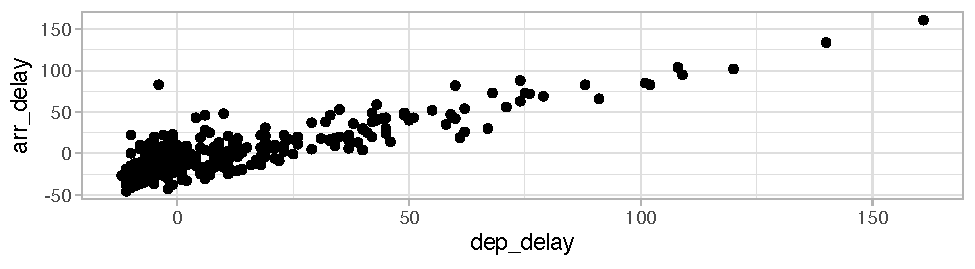
\includegraphics[width=\textwidth]{ModernDive_files/figure-latex/noalpha-1} 

}

\caption{Arrival delays versus departure delays for Envoy Air flights from NYC in 2023.}\label{fig:noalpha}
\end{figure}

Let's first unpack the graphic in Figure \ref{fig:noalpha}. Observe that a \emph{positive relationship} exists between \texttt{dep\_delay} and \texttt{arr\_delay}: as departure delays increase, arrival delays tend to also increase. Observe also the large mass of points clustered near (0, 0), the point indicating flights that neither departed nor arrived late.

Let's turn our attention to the warning message. R is alerting us to the fact that three rows were ignored due to them being missing. For these three rows, either the value for \texttt{dep\_delay} or \texttt{arr\_delay} or both were missing (recorded in R as \texttt{NA}), and thus these rows were ignored in our plot.

Before we continue, let's make a few more observations about this code that created the scatterplot. Note that the \texttt{+} sign comes at the end of lines, and not at the beginning. You'll get an error in R if you put it at the beginning of a line. \index{R packages!ggplot2!+} When adding layers to a plot, you are encouraged to start a new line after the \texttt{+} (by pressing the Return/Enter button on your keyboard) so that the code for each layer is on a new line. As we add more and more layers to plots, you'll see this will greatly improve the legibility of your code.

To stress the importance of adding the layer specifying the \texttt{geom}etric object, consider Figure \ref{fig:nolayers} where no layers are added. Because the \texttt{geom}etric object was not specified, we have a blank plot that is not very useful!

\begin{Shaded}
\begin{Highlighting}[]
\FunctionTok{ggplot}\NormalTok{(}\AttributeTok{data =}\NormalTok{ envoy\_flights, }\AttributeTok{mapping =} \FunctionTok{aes}\NormalTok{(}\AttributeTok{x =}\NormalTok{ dep\_delay, }\AttributeTok{y =}\NormalTok{ arr\_delay))}
\end{Highlighting}
\end{Shaded}

\begin{figure}[H]

{\centering 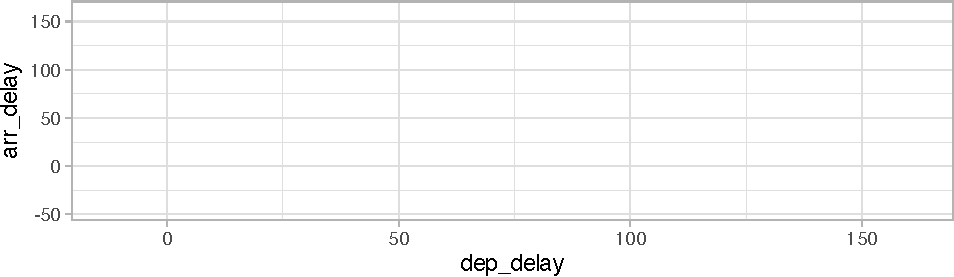
\includegraphics[width=\textwidth]{ModernDive_files/figure-latex/nolayers-1} 

}

\caption{A plot with no layers.}\label{fig:nolayers}
\end{figure}

\begin{learncheck}
\vspace{-0.15in}

\textbf{\emph{Learning check}} \vspace{-0.1in}
\end{learncheck}

\textbf{(LC2.2)} What are practical reasons why \texttt{dep\_delay} and \texttt{arr\_delay} have a positive relationship?

\textbf{(LC2.3)} What variables in the \texttt{weather} data frame would you expect to have a negative correlation (i.e., a negative relationship) with \texttt{dep\_delay}? Why? Remember that we are focusing on numerical variables here. Hint: Explore the \texttt{weather} dataset by using the \texttt{View()} function.

\textbf{(LC2.4)} Why do you believe there is a cluster of points near (0, 0)? What does (0, 0) correspond to in terms of the Envoy Air flights?

\textbf{(LC2.5)} What are some other features of the plot that stand out to you?

\textbf{(LC2.6)} Create a new scatterplot using different variables in the \texttt{envoy\_flights} data frame by modifying the example given.

\begin{learncheck}
\vspace{-0.25in}
\vspace{-0.25in}
\end{learncheck}

\subsection{Overplotting}\label{overplotting}

The large mass of points near (0, 0) in Figure \ref{fig:noalpha} can cause some confusion since it is hard to tell the true number of points that are plotted. This is the result of a phenomenon called \index{overplotting} \emph{overplotting}. As one may guess, this corresponds to points being plotted on top of each other over and over again. When overplotting occurs, it is difficult to know the number of points being plotted. There are two methods to address the issue of overplotting. Either by

\begin{enumerate}
\def\labelenumi{\arabic{enumi}.}
\tightlist
\item
  Adjusting the transparency of the points or
\item
  Adding a little random ``jitter'', or random ``nudges'', to each of the points.
\end{enumerate}

\textbf{Method 1: Changing the transparency}

The first way of addressing overplotting is to change the transparency/opacity of the points by setting the \texttt{alpha} argument in \texttt{geom\_point()}. We can change the \texttt{alpha} argument to be any value between \texttt{0} and \texttt{1}, where \texttt{0} sets the points to be 100\% transparent and \texttt{1} sets the points to be 100\% opaque. By default, \texttt{alpha} is set to \texttt{1}. In other words, if we don't explicitly set an \texttt{alpha} value, R will use \texttt{alpha\ =\ 1}.

Note how the following code is identical to the code in Section \ref{scatterplots} that created the scatterplot with overplotting, but with \texttt{alpha\ =\ 0.2} added to the \texttt{geom\_point()} function:

\begin{Shaded}
\begin{Highlighting}[]
\FunctionTok{ggplot}\NormalTok{(}\AttributeTok{data =}\NormalTok{ envoy\_flights, }\AttributeTok{mapping =} \FunctionTok{aes}\NormalTok{(}\AttributeTok{x =}\NormalTok{ dep\_delay, }\AttributeTok{y =}\NormalTok{ arr\_delay)) }\SpecialCharTok{+} 
  \FunctionTok{geom\_point}\NormalTok{(}\AttributeTok{alpha =} \FloatTok{0.2}\NormalTok{)}
\end{Highlighting}
\end{Shaded}

\begin{figure}[H]

{\centering 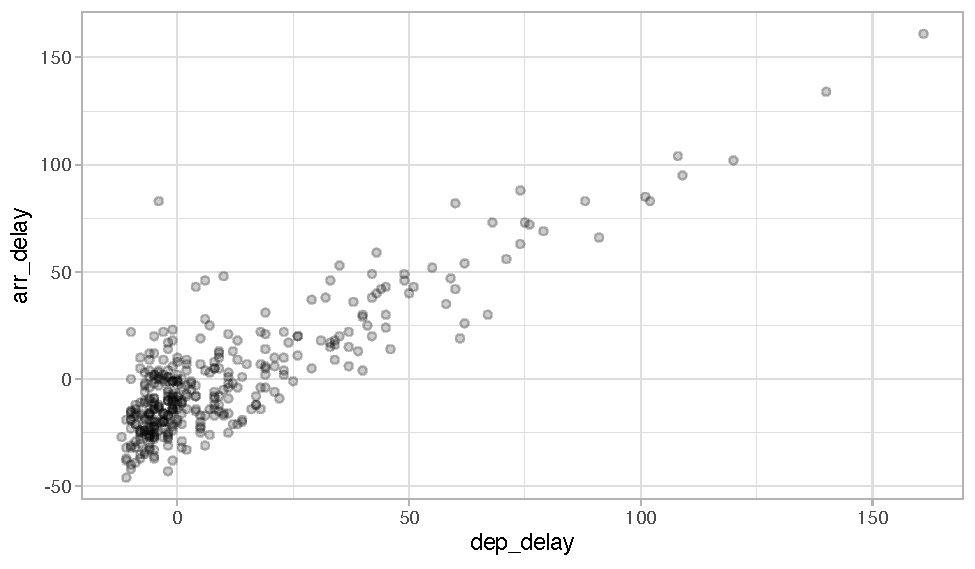
\includegraphics[width=\textwidth]{ModernDive_files/figure-latex/alpha-1} 

}

\caption{Arrival vs. departure delays scatterplot with alpha = 0.2.}\label{fig:alpha}
\end{figure}

The key feature to note in Figure \ref{fig:alpha} is that the transparency \index{R packages!ggplot2!alpha}\index{adding transparency to plots}of the points is cumulative: areas with a high-degree of overplotting are darker, whereas areas with a lower degree are less dark. Note furthermore that there is no \texttt{aes()} surrounding \texttt{alpha\ =\ 0.2}. This is because we are not mapping a variable to an aesthetic attribute, but rather merely changing the default setting of \texttt{alpha}. In fact, you'll receive an error if you try to change the second line to read \texttt{geom\_point(aes(alpha\ =\ 0.2))}.

\textbf{Method 2: Jittering the points}

The second way of addressing overplotting is by \emph{jittering} all the points. This means giving each point a small ``nudge'' in a random direction. You can think of ``jittering'' as shaking the points around a bit on the plot. Let's illustrate using a simple example first. Say we have a data frame with 4 identical rows of x and y values: (0,0), (0,0), (0,0), and (0,0). In Figure \ref{fig:jitter-example-plot-1}, we present both the regular scatterplot of these 4 points (on the left) and its jittered counterpart (on the right).

\begin{figure}[H]

{\centering 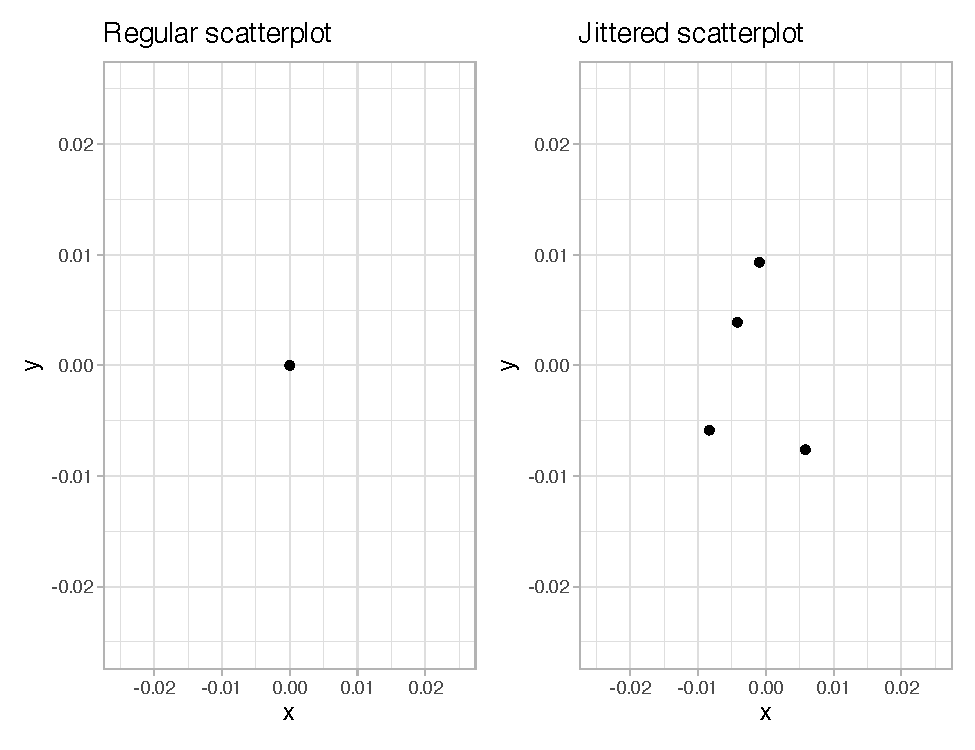
\includegraphics[width=\textwidth]{ModernDive_files/figure-latex/jitter-example-plot-1-1} 

}

\caption{Regular and jittered scatterplot.}\label{fig:jitter-example-plot-1}
\end{figure}

In the left-hand regular scatterplot, observe that the 4 points are superimposed on top of each other. While we know there are 4 values being plotted, this fact might not be apparent to others. In the right-hand jittered scatterplot, it is now plainly evident that this plot involves four points since each point is given a random ``nudge.''

Keep in mind, however, that jittering is strictly a visualization tool; even after creating a jittered scatterplot, the original values saved in the data frame remain unchanged. \index{R packages!ggplot2!geom\_jitter()}

To create a jittered scatterplot, instead of using \texttt{geom\_point()}, we use \texttt{geom\_jitter()}. Observe how the following code is very similar to the code that created the scatterplot with overplotting in Subsection \ref{geompoint}, but with \texttt{geom\_point()} \index{R packages!ggplot2!geom\_point()} replaced with \texttt{geom\_jitter()}.

\begin{Shaded}
\begin{Highlighting}[]
\FunctionTok{ggplot}\NormalTok{(}\AttributeTok{data =}\NormalTok{ envoy\_flights, }\AttributeTok{mapping =} \FunctionTok{aes}\NormalTok{(}\AttributeTok{x =}\NormalTok{ dep\_delay, }\AttributeTok{y =}\NormalTok{ arr\_delay)) }\SpecialCharTok{+} 
  \FunctionTok{geom\_jitter}\NormalTok{(}\AttributeTok{width =} \DecValTok{30}\NormalTok{, }\AttributeTok{height =} \DecValTok{30}\NormalTok{)}
\end{Highlighting}
\end{Shaded}

\begin{figure}[H]

{\centering 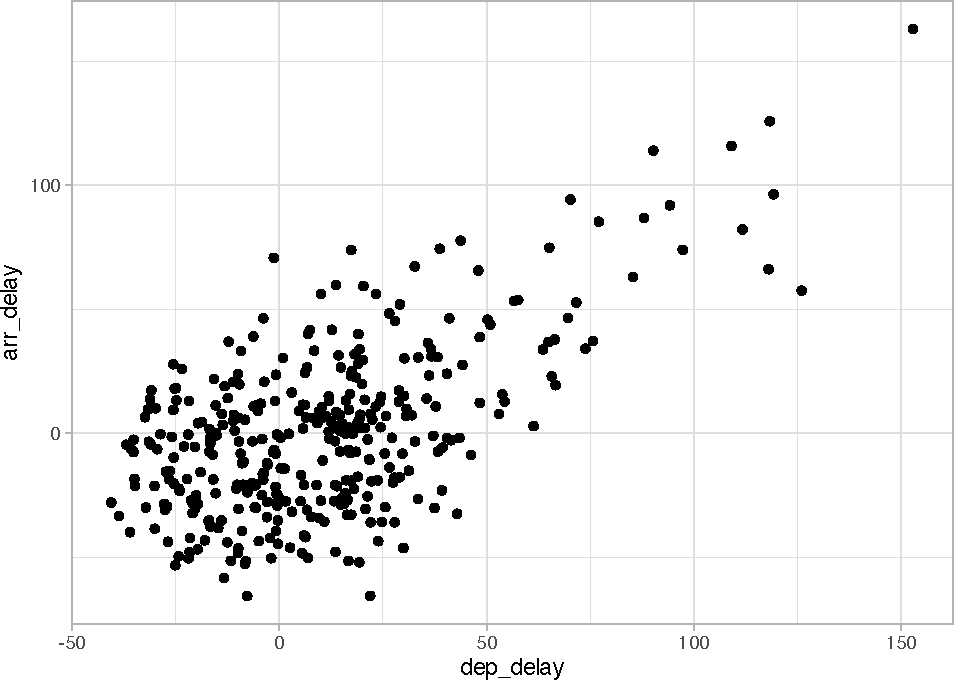
\includegraphics[width=\textwidth]{ModernDive_files/figure-latex/jitter-1} 

}

\caption{Arrival versus departure delays jittered scatterplot.}\label{fig:jitter}
\end{figure}

In order to specify how much jitter to add, we adjusted the \texttt{width} and \texttt{height} arguments to \texttt{geom\_jitter()}. This corresponds to how hard you'd like to shake the plot in horizontal x-axis units and vertical y-axis units, respectively. In this case, both axes are in minutes. How much jitter should we add using the \texttt{width} and \texttt{height} arguments? On the one hand, it is important to add just enough jitter to break any overlap in points, but on the other hand, not so much that we completely alter the original pattern in points.

As can be seen in the resulting Figure \ref{fig:jitter}, in this case jittering doesn't really provide much new insight. In this particular case, it can be argued that changing the transparency of the points by setting \texttt{alpha} proved more effective. When would it be better to use a jittered scatterplot? When would it be better to alter the points' transparency? There is no single right answer that applies to all situations. You need to make a subjective choice and own that choice. At the very least when confronted with overplotting, however, we suggest you make both types of plots and see which one better emphasizes the point you are trying to make.

\begin{learncheck}
\vspace{-0.15in}

\textbf{\emph{Learning check}} \vspace{-0.1in}
\end{learncheck}

\textbf{(LC2.7)} Why is setting the \texttt{alpha} argument value useful with scatterplots? What further information does it give you that a regular scatterplot cannot?

\textbf{(LC2.8)} After viewing Figure \ref{fig:alpha}, give an approximate range of arrival delays and departure delays that occur most frequently. How has that region changed compared to when you observed the same plot without \texttt{alpha\ =\ 0.2} set in Figure \ref{fig:noalpha}?

\begin{learncheck}
\vspace{-0.25in}
\vspace{-0.25in}
\end{learncheck}

\subsection{Summary}\label{summary}

Scatterplots display the relationship between two numerical variables. They are among the most commonly used plots because they can provide an immediate way to see the trend in one numerical variable versus another. However, if you try to create a scatterplot where either one of the two variables is not numerical, you might get strange results. Be careful!

With medium to large datasets, you may need to play around with the different modifications to scatterplots we saw such as changing the transparency/opacity of the points or by jittering the points. This tweaking is often a fun part of data visualization, since you'll have the chance to see different relationships emerge as you tinker with your plots.

\section{5NG\#2: Linegraphs}\label{linegraphs}

The next of the five named graphs are linegraphs. Linegraphs \index{linegraphs} show the relationship between two numerical variables when the variable on the x-axis, also called the \emph{explanatory} variable\index{explanatory variable}, is of a sequential nature. In other words, there is an inherent ordering to the variable.

The most common examples of linegraphs have some notion of time on the x-axis: hours, days, weeks, years, etc. Since time is sequential, we connect consecutive observations of the variable on the y-axis with a line. Linegraphs that have some notion of time on the x-axis are also called \emph{time series} plots\index{time series plots}. Let's illustrate linegraphs using another dataset in the \texttt{nycflights23} \index{R packages!nycflights23} package: the \texttt{weather} data frame.

Let's explore the \texttt{weather} data frame from the \texttt{nycflights23} package by running \texttt{View(weather)} and \texttt{glimpse(weather)}. Furthermore let's read the associated help file by running \texttt{?weather} to bring up the help file.

Observe that there is a variable called \texttt{temp} of hourly wind speed recordings in miles per hour at weather stations near all three major airports in New York City: Newark (\texttt{origin} code \texttt{EWR}), John F. Kennedy International (\texttt{JFK}), and LaGuardia (\texttt{LGA}).

However, instead of considering hourly wind speeds for all days in 2023 for all three airports, for simplicity let's only consider hourly wind speeds at Newark airport for the first 15 days in January. This data is accessible in the \texttt{early\_january\_2023\_weather} data frame included in the \texttt{moderndive} package. In other words, \texttt{early\_january\_2023\_weather} contains hourly weather observations for \texttt{origin} equal to \texttt{EWR} (Newark's airport code), \texttt{month} equal to \texttt{1}, and \texttt{day} less than or equal to \texttt{15}.

\begin{learncheck}
\vspace{-0.15in}

\textbf{\emph{Learning check}} \vspace{-0.1in}
\end{learncheck}

\textbf{(LC2.9)} Take a look at both the \texttt{weather} data frame from the \texttt{nycflights23} package and the \texttt{early\_january\_2023\_weather} data frame from the \texttt{moderndive} package by running \texttt{View(weather)} and \texttt{View(early\_january\_2023\_weather)}. In what respect do these data frames differ?

\textbf{(LC2.10)} \texttt{View()} the \texttt{flights} data frame again. Why does the \texttt{time\_hour} variable uniquely identify the hour of the measurement, whereas the \texttt{hour} variable does not?

\begin{learncheck}
\vspace{-0.25in}
\vspace{-0.25in}
\end{learncheck}

\subsection{\texorpdfstring{Linegraphs via \texttt{geom\_line}}{Linegraphs via geom\_line}}\label{geomline}

Let's create a time series plot of the hourly wind speeds saved in the \texttt{early\_january\_2023\_weather} data frame by using \texttt{geom\_line()} to create a linegraph\index{R packages!ggplot2!geom\_line()}, instead of using \texttt{geom\_point()} like we used previously to create scatterplots:

\begin{Shaded}
\begin{Highlighting}[]
\FunctionTok{ggplot}\NormalTok{(}\AttributeTok{data =}\NormalTok{ early\_january\_2023\_weather, }
       \AttributeTok{mapping =} \FunctionTok{aes}\NormalTok{(}\AttributeTok{x =}\NormalTok{ time\_hour, }\AttributeTok{y =}\NormalTok{ wind\_speed)) }\SpecialCharTok{+}
  \FunctionTok{geom\_line}\NormalTok{()}
\end{Highlighting}
\end{Shaded}

\begin{figure}[H]

{\centering 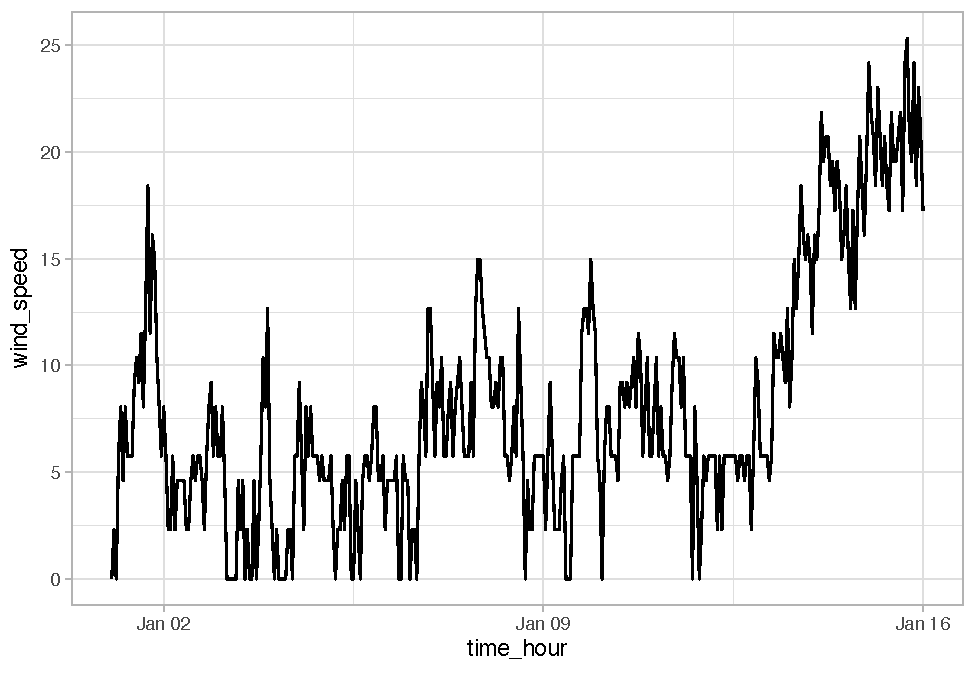
\includegraphics[width=\textwidth]{ModernDive_files/figure-latex/hourlytemp-1} 

}

\caption{Hourly wind speed in Newark for January 1-15, 2023.}\label{fig:hourlytemp}
\end{figure}

Much as with the \texttt{ggplot()} code that created the scatterplot of departure and arrival delays for Envoy Air flights in Figure \ref{fig:noalpha}, let's break down this code piece-by-piece in terms of the grammar of graphics:

Within the \texttt{ggplot()} function call, we specify two of the components of the grammar of graphics as arguments:

\begin{enumerate}
\def\labelenumi{\arabic{enumi}.}
\tightlist
\item
  The \texttt{data} to be the \texttt{early\_january\_2023\_weather} data frame by setting \texttt{data\ =\ early\_january\_2023\_weather}.
\item
  The \texttt{aes}thetic \texttt{mapping} by setting \texttt{mapping\ =\ aes(x\ =\ time\_hour,\ y\ =\ temp)}. Specifically, the variable \texttt{time\_hour} maps to the \texttt{x} position aesthetic, while the variable \texttt{wind\_speed} maps to the \texttt{y} position aesthetic.
\end{enumerate}

We add a layer to the \texttt{ggplot()} function call using the \texttt{+} sign. The layer in question specifies the third component of the grammar: the \texttt{geom}etric object in question. In this case, the geometric object is a \texttt{line} set by specifying \texttt{geom\_line()}.

\begin{learncheck}
\vspace{-0.15in}

\textbf{\emph{Learning check}} \vspace{-0.1in}
\end{learncheck}

\textbf{(LC2.11)} Why should linegraphs be avoided when there is not a clear ordering of the horizontal axis?

\textbf{(LC2.12)} Why are linegraphs frequently used when time is the explanatory variable on the x-axis?

\textbf{(LC2.13)} Plot a time series of a variable other than \texttt{wind\_speed} for Newark Airport in the first 15 days of January 2023. Try to select a variable that doesn't have a lot of missing (\texttt{NA}) values.

\begin{learncheck}
\vspace{-0.25in}
\vspace{-0.25in}
\end{learncheck}

\subsection{Summary}\label{summary-1}

Linegraphs, just like scatterplots, display the relationship between two numerical variables. However, it is preferred to use linegraphs over scatterplots when the variable on the x-axis (i.e., the explanatory variable) has an inherent ordering, such as some notion of time.

\section{5NG\#3: Histograms}\label{histograms}

Let's consider the \texttt{wind\_speed} variable in the \texttt{weather} data frame once again, but unlike with the linegraphs in Section \ref{linegraphs}, let's say we don't care about its relationship with time, but rather we only care about how the values of \texttt{wind\_speed} \emph{distribute}. In other words:

\begin{enumerate}
\def\labelenumi{\arabic{enumi}.}
\tightlist
\item
  What are the smallest and largest values?
\item
  What is the ``center'' or ``most typical'' value?
\item
  How do the values spread out?
\item
  What are frequent and infrequent values?
\end{enumerate}

One way to visualize this \emph{distribution} \index{distribution} of this single variable \texttt{wind\_speed} is to plot them on a horizontal line as we do in Figure \ref{fig:windspeed-on-line}:

\begin{figure}[H]

{\centering 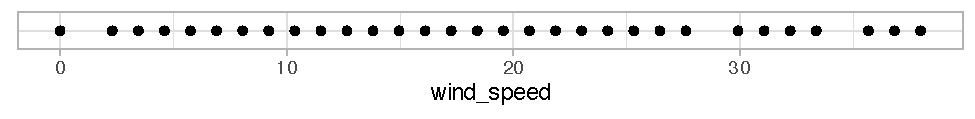
\includegraphics[width=\textwidth]{ModernDive_files/figure-latex/windspeed-on-line-1} 

}

\caption{Plot of hourly wind speed recordings from NYC in 2023.}\label{fig:windspeed-on-line}
\end{figure}

This gives us a general idea of how the values of \texttt{wind\_speed} distribute: observe that wind speeds vary from around 0 miles per hour (0 kilometers per hour ) up to 38 miles per hour (approximately 61 kilometers per hour). There appear to be more recorded wind speeds between 0 and 20 miles per hour (mph) than outside this range. However, because of the high degree of overplotting in the points, it's hard to get a sense of exactly how many values are between, say, 10 mph and 15 mph.

What is commonly produced instead of Figure \ref{fig:windspeed-on-line} is known as a \index{histograms} \emph{histogram}. A histogram is a plot that visualizes the \emph{distribution} of a numerical value as follows:

\begin{enumerate}
\def\labelenumi{\arabic{enumi}.}
\tightlist
\item
  We first cut up the x-axis into a series of \index{histograms!bins} \emph{bins}, where each bin represents a range of values.
\item
  For each bin, we count the number of observations that fall in the range corresponding to that bin.
\item
  Then for each bin, we draw a bar whose height marks the corresponding count.
\end{enumerate}

Let's drill-down on an example of a histogram, shown in Figure \ref{fig:histogramexample}.

\begin{figure}[H]

{\centering 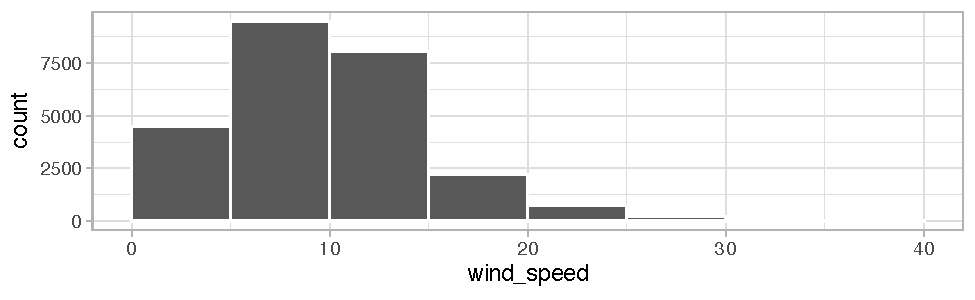
\includegraphics[width=\textwidth]{ModernDive_files/figure-latex/histogramexample-1} 

}

\caption{Example histogram.}\label{fig:histogramexample}
\end{figure}

Let's focus only on wind speeds between 10 mph and 25 mph for now. Observe that there are three bins of equal width between 10 mph and 25 mph. Thus we have three bins of width 5 mph each: one bin for the 10-15 mph range, another bin for the 15-20 mph range, and another bin for the 20-25 mph range. Since:

\begin{enumerate}
\def\labelenumi{\arabic{enumi}.}
\tightlist
\item
  The bin for the 10-15 mph range has a height of around 8000. In other words, around 8000 of the hourly wind speed recordings are between 10 mph and 15 mph.
\item
  The bin for the 15-20 mph range has a height of around 2400. In other words, around 2400 of the hourly wind speed recordings are between 15 mph and 20 mph.
\item
  The bin for the 20-25 mph range has a height of around 700. In other words, around 700 of the hourly wind speed recordings are between 20 mph and 25 mph.
\end{enumerate}

All eight bins spanning 0 mph to 40 mph on the x-axis have this interpretation.

\subsection{\texorpdfstring{Histograms via \texttt{geom\_histogram}}{Histograms via geom\_histogram}}\label{geomhistogram}

Let's now present the \texttt{ggplot()} code to plot your first histogram! Unlike with scatterplots and linegraphs, there is now only one variable being mapped in \texttt{aes()}: the single numerical variable \texttt{wind\_speed}. The y-aesthetic of a histogram, the count of the observations in each bin, gets computed for you automatically. Furthermore, the geometric object layer is now a \texttt{geom\_histogram()}. \index{R packages!ggplot2!geom\_histogram()} After running the following code, you'll see the histogram in Figure \ref{fig:weather-histogram} as well as warning messages. We'll discuss the warning messages first.

\begin{Shaded}
\begin{Highlighting}[]
\FunctionTok{ggplot}\NormalTok{(}\AttributeTok{data =}\NormalTok{ weather, }\AttributeTok{mapping =} \FunctionTok{aes}\NormalTok{(}\AttributeTok{x =}\NormalTok{ wind\_speed)) }\SpecialCharTok{+}
  \FunctionTok{geom\_histogram}\NormalTok{()}
\end{Highlighting}
\end{Shaded}

\begin{verbatim}
`stat_bin()` using `bins = 30`. Pick better value with `binwidth`.
\end{verbatim}

\begin{verbatim}
Warning: Removed 1033 rows containing non-finite outside the scale range
(`stat_bin()`).
\end{verbatim}

\begin{figure}[H]

{\centering 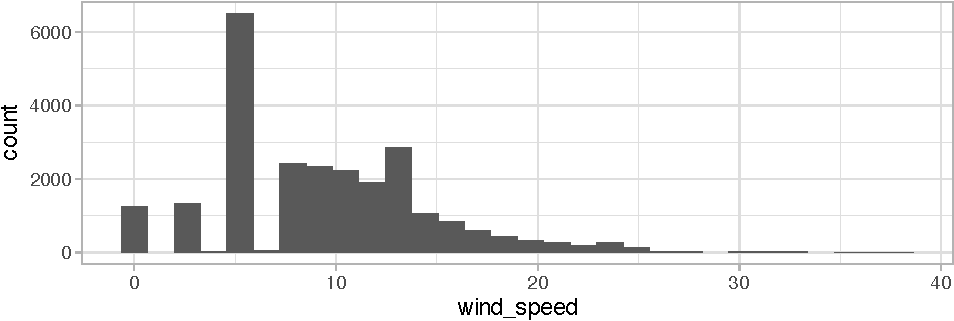
\includegraphics[width=\textwidth]{ModernDive_files/figure-latex/weather-histogram-1} 

}

\caption{Histogram of hourly wind speeds at three NYC airports.}\label{fig:weather-histogram}
\end{figure}

The first message is telling us that the histogram was constructed using \texttt{bins\ =\ 30} for 30 equally spaced bins. This is known in computer programming as a default value; unless you override this default number of bins with a number you specify, R will choose 30 by default. We'll see in the next section how to change the number of bins to another value than the default.

The second message is telling us something similar to the warning message we received when we ran the code to create a scatterplot of departure and arrival delays for Envoy Air flights in Figure \ref{fig:noalpha}: that because some rows have missing \texttt{NA} value for \texttt{wind\_speed}, they were omitted from the histogram. R is just giving us a friendly heads-up that this was the case.

Now let's unpack the resulting histogram in Figure \ref{fig:weather-histogram}. Observe that values above 30 mph are rather rare. However, because of the large number of bins, it's hard to get a sense for which range of wind speeds is spanned by each bin; everything is one giant amorphous blob. So let's add white vertical borders demarcating the bins by adding a \texttt{color\ =\ "white"} argument to \texttt{geom\_histogram()} and ignore the warning about setting the number of bins to a better value:

\begin{Shaded}
\begin{Highlighting}[]
\FunctionTok{ggplot}\NormalTok{(}\AttributeTok{data =}\NormalTok{ weather, }\AttributeTok{mapping =} \FunctionTok{aes}\NormalTok{(}\AttributeTok{x =}\NormalTok{ wind\_speed)) }\SpecialCharTok{+}
  \FunctionTok{geom\_histogram}\NormalTok{(}\AttributeTok{color =} \StringTok{"white"}\NormalTok{)}
\end{Highlighting}
\end{Shaded}

\begin{figure}[H]

{\centering 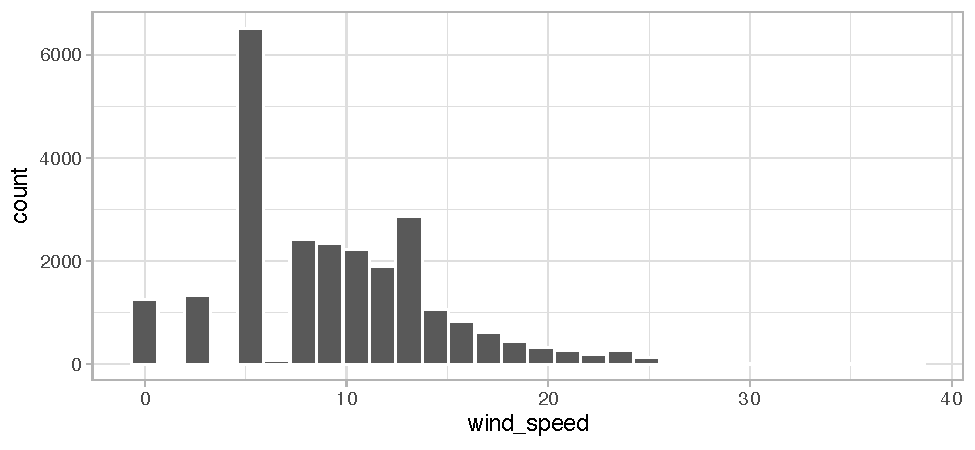
\includegraphics[width=\textwidth]{ModernDive_files/figure-latex/weather-histogram-2-1} 

}

\caption{Histogram of hourly wind speeds at three NYC airports with white borders.}\label{fig:weather-histogram-2}
\end{figure}

We now have an easier time associating ranges of wind speeds to each of the bins in Figure \ref{fig:weather-histogram-2}. We can also vary the color of the bars by setting the \index{R packages!ggplot2!fill} \texttt{fill} argument. For example, you can set the bin colors to be ``blue steel'' by setting \texttt{fill\ =\ "steelblue"}:

\begin{Shaded}
\begin{Highlighting}[]
\FunctionTok{ggplot}\NormalTok{(}\AttributeTok{data =}\NormalTok{ weather, }\AttributeTok{mapping =} \FunctionTok{aes}\NormalTok{(}\AttributeTok{x =}\NormalTok{ wind\_speed)) }\SpecialCharTok{+}
  \FunctionTok{geom\_histogram}\NormalTok{(}\AttributeTok{color =} \StringTok{"white"}\NormalTok{, }\AttributeTok{fill =} \StringTok{"steelblue"}\NormalTok{)}
\end{Highlighting}
\end{Shaded}

If you're curious, run \index{colors()} \texttt{colors()} to see all 657 possible choice of colors in R!

\subsection{Adjusting the bins}\label{adjustbins}

Observe in Figure \ref{fig:weather-histogram-2} that in the 10-20 mph range there appear to be roughly 8 bins. Thus each bin has width 10 divided by 8, or 1.125 mph, which is not a very easily interpretable range to work with. Let's improve this by adjusting the number of bins in our histogram in one of two ways:

\begin{enumerate}
\def\labelenumi{\arabic{enumi}.}
\tightlist
\item
  By adjusting the number of bins via the \index{R packages!ggplot2|geom\_histogram()!bins} \texttt{bins} argument to \texttt{geom\_histogram()}.
\item
  By adjusting the width of the bins via the \index{R packages!ggplot2|geom\_histogram()!binwidth} \texttt{binwidth} argument to \texttt{geom\_histogram()}.
\end{enumerate}

Using the first method, we have the power to specify how many bins we would like to cut the x-axis up in. As mentioned in the previous section, the default number of bins is 20. We can override this default, to say 20 bins, as follows:

\begin{Shaded}
\begin{Highlighting}[]
\FunctionTok{ggplot}\NormalTok{(}\AttributeTok{data =}\NormalTok{ weather, }\AttributeTok{mapping =} \FunctionTok{aes}\NormalTok{(}\AttributeTok{x =}\NormalTok{ wind\_speed)) }\SpecialCharTok{+}
  \FunctionTok{geom\_histogram}\NormalTok{(}\AttributeTok{bins =} \DecValTok{20}\NormalTok{, }\AttributeTok{color =} \StringTok{"white"}\NormalTok{)}
\end{Highlighting}
\end{Shaded}

Using the second method, instead of specifying the number of bins, we specify the width of the bins by using the \texttt{binwidth} argument in the \texttt{geom\_histogram()} layer. For example, let's set the width of each bin to be five mph.

\begin{Shaded}
\begin{Highlighting}[]
\FunctionTok{ggplot}\NormalTok{(}\AttributeTok{data =}\NormalTok{ weather, }\AttributeTok{mapping =} \FunctionTok{aes}\NormalTok{(}\AttributeTok{x =}\NormalTok{ wind\_speed)) }\SpecialCharTok{+}
  \FunctionTok{geom\_histogram}\NormalTok{(}\AttributeTok{binwidth =} \DecValTok{5}\NormalTok{, }\AttributeTok{color =} \StringTok{"white"}\NormalTok{)}
\end{Highlighting}
\end{Shaded}

We compare both resulting histograms side-by-side in Figure \ref{fig:hist-bins}.

\begin{figure}[H]

{\centering 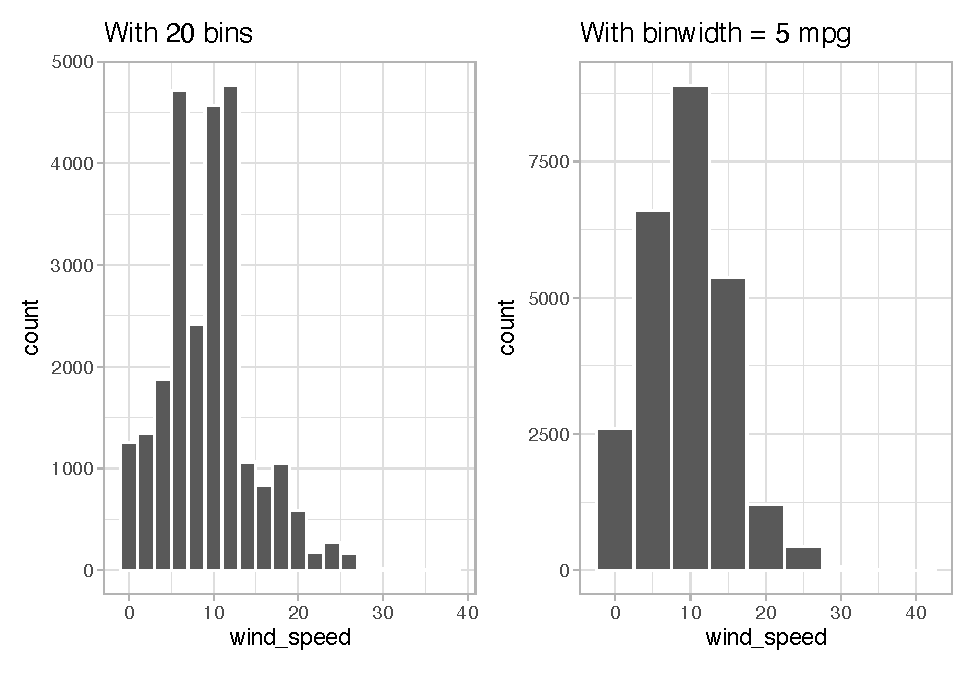
\includegraphics[width=\textwidth]{ModernDive_files/figure-latex/hist-bins-1} 

}

\caption{Setting histogram bins in two ways.}\label{fig:hist-bins}
\end{figure}

\begin{learncheck}
\vspace{-0.15in}

\textbf{\emph{Learning check}} \vspace{-0.1in}
\end{learncheck}

\textbf{(LC2.14)} What does changing the number of bins from 30 to 20 tell us about the distribution of wind speeds?

\textbf{(LC2.15)} Would you classify the distribution of wind speeds as symmetric or skewed in one direction or another?

\textbf{(LC2.16)} What would you guess is the ``center'' value in this distribution? Why did you make that choice?

\textbf{(LC2.17)} Is this data spread out greatly from the center or is it close? Why?

\begin{learncheck}
\vspace{-0.25in}
\vspace{-0.25in}
\end{learncheck}

\subsection{Summary}\label{summary-2}

Histograms, unlike scatterplots and linegraphs, present information on only a single numerical variable. Specifically, they are visualizations of the distribution of the numerical variable in question.

\section{Facets}\label{facets}

Before continuing with the next of the 5NG, let's briefly introduce a new concept called \emph{faceting}. Faceting is used when we'd like to split a particular visualization by the values of another variable. This will create multiple copies of the same type of plot with matching x and y axes, but whose content will differ.

For example, suppose we were interested in looking at how the histogram of hourly wind speed recordings at the three NYC airports we saw in Figure \ref{fig:histogramexample} differed in each month. We could ``split'' this histogram by the 12 possible months in a given year. In other words, we would plot histograms of \texttt{wind\_speed} for each \texttt{month} separately. We do this by adding \texttt{facet\_wrap(\textasciitilde{}\ month)} layer. Note the \texttt{\textasciitilde{}} is a ``tilde'' and can generally be found on the key next to the ``1'' key on US keyboards. The tilde is required and you'll receive the error \texttt{Error\ in\ as.quoted(facets)\ :\ object\ \textquotesingle{}month\textquotesingle{}\ not\ found} if you don't include it here.

\begin{Shaded}
\begin{Highlighting}[]
\FunctionTok{ggplot}\NormalTok{(}\AttributeTok{data =}\NormalTok{ weather, }\AttributeTok{mapping =} \FunctionTok{aes}\NormalTok{(}\AttributeTok{x =}\NormalTok{ wind\_speed)) }\SpecialCharTok{+}
  \FunctionTok{geom\_histogram}\NormalTok{(}\AttributeTok{binwidth =} \DecValTok{5}\NormalTok{, }\AttributeTok{color =} \StringTok{"white"}\NormalTok{) }\SpecialCharTok{+}
  \FunctionTok{facet\_wrap}\NormalTok{(}\SpecialCharTok{\textasciitilde{}}\NormalTok{ month)}
\end{Highlighting}
\end{Shaded}

\begin{figure}[H]

{\centering 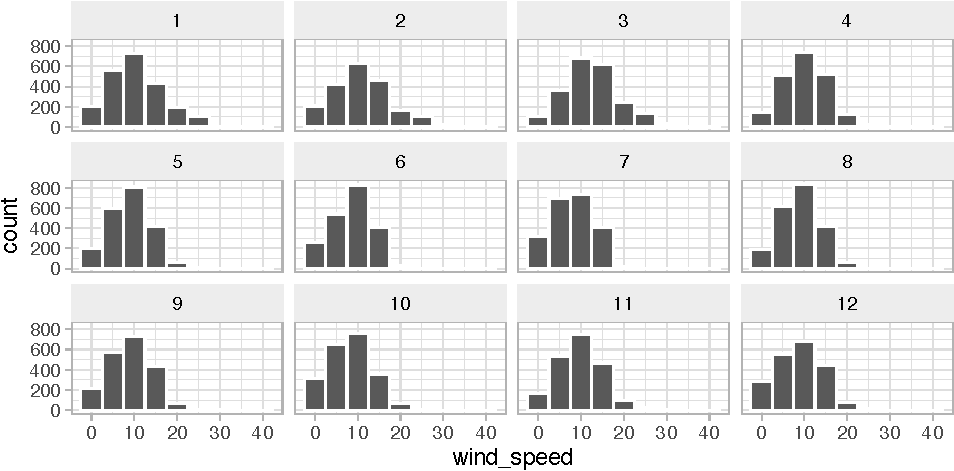
\includegraphics[width=\textwidth]{ModernDive_files/figure-latex/facethistogram-1} 

}

\caption{Faceted histogram of hourly wind speeds by month.}\label{fig:facethistogram}
\end{figure}

We can also specify the number of rows and columns in the grid by using the \texttt{nrow} and \texttt{ncol} arguments inside of \index{R packages!ggplot2!facet\_wrap()} \texttt{facet\_wrap()}. For example, say we would like our faceted histogram to have 4 rows instead of 3. We simply add an \texttt{nrow\ =\ 4} argument to \texttt{facet\_wrap(\textasciitilde{}\ month)}.

\begin{Shaded}
\begin{Highlighting}[]
\FunctionTok{ggplot}\NormalTok{(}\AttributeTok{data =}\NormalTok{ weather, }\AttributeTok{mapping =} \FunctionTok{aes}\NormalTok{(}\AttributeTok{x =}\NormalTok{ wind\_speed)) }\SpecialCharTok{+}
  \FunctionTok{geom\_histogram}\NormalTok{(}\AttributeTok{binwidth =} \DecValTok{5}\NormalTok{, }\AttributeTok{color =} \StringTok{"white"}\NormalTok{) }\SpecialCharTok{+}
  \FunctionTok{facet\_wrap}\NormalTok{(}\SpecialCharTok{\textasciitilde{}}\NormalTok{ month, }\AttributeTok{nrow =} \DecValTok{4}\NormalTok{)}
\end{Highlighting}
\end{Shaded}

\begin{figure}[H]

{\centering 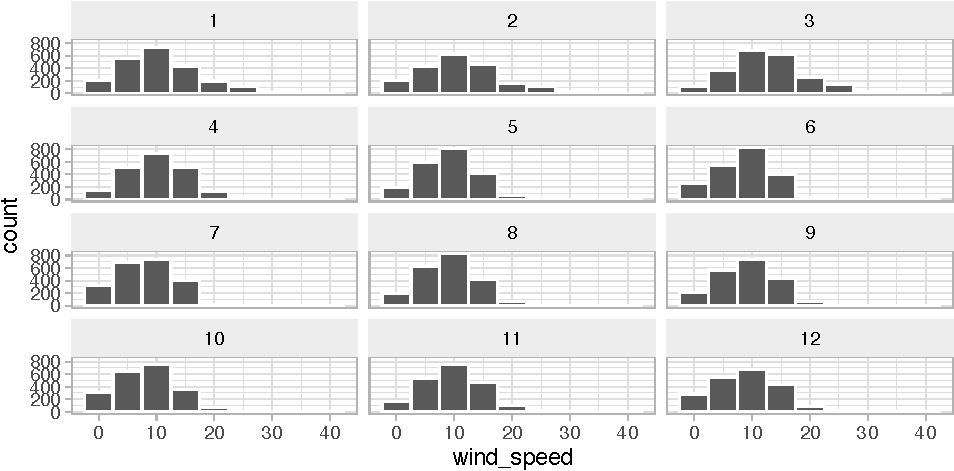
\includegraphics[width=\textwidth]{ModernDive_files/figure-latex/facethistogram2-1} 

}

\caption{Faceted histogram with 4 instead of 3 rows.}\label{fig:facethistogram2}
\end{figure}

Observe in both Figures \ref{fig:facethistogram} and \ref{fig:facethistogram2} the majority of wind speed observations for all months are clustered between 0 and 20 mph, with very few observations exceeding 30 mph.
The histograms show a similar shape across months, with most distributions having a similar largest count and a few larger speed outliers, indicating that lower wind speeds are more common than higher wind speeds.

\begin{learncheck}
\vspace{-0.15in}

\textbf{\emph{Learning check}} \vspace{-0.1in}
\end{learncheck}

\textbf{(LC2.18)} What other things do you notice about this faceted plot? How does a faceted plot help us see relationships between two variables?

\textbf{(LC2.19)} What do the numbers 1-12 correspond to in the plot? What about 10, 20, and 30?

\textbf{(LC2.20)} For which types of datasets would faceted plots not work well in comparing relationships between variables? Give an example describing the nature of these variables and other important characteristics.

\textbf{(LC2.21)} Does the \texttt{wind\_speed} variable in the \texttt{weather} dataset have a lot of variability? Why do you say that?

\begin{learncheck}
\vspace{-0.25in}
\vspace{-0.25in}
\end{learncheck}

\section{5NG\#4: Boxplots}\label{boxplots}

While faceted histograms are one type of visualization used to compare the distribution of a numerical variable split by the values of another variable, another type of visualization that achieves this same goal is a \emph{side-by-side boxplot}. A boxplot \index{boxplots} is constructed from the information provided in the \emph{five-number summary} of a numerical variable. To keep things simple for now, let's only consider the 2057 recorded hourly wind speed recordings for the month of April, each represented as a jittered point in Figure \ref{fig:apr1}.

\begin{figure}[H]

{\centering 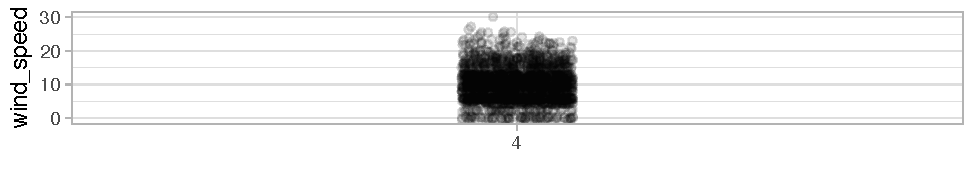
\includegraphics[width=\textwidth]{ModernDive_files/figure-latex/apr1-1} 

}

\caption{April wind speeds represented as jittered points.}\label{fig:apr1}
\end{figure}

These 2057 observations have the following \emph{five-number summary}:

\begin{enumerate}
\def\labelenumi{\arabic{enumi}.}
\tightlist
\item
  Minimum: 0 mph
\item
  First quartile (25th percentile): 5.8 mph
\item
  Median (second quartile, 50th percentile): 9.2 mph
\item
  Third quartile (75th percentile): 12.7 mph
\item
  Maximum: 29.92 mph
\end{enumerate}

In the leftmost plot of Figure \ref{fig:apr2}, let's mark these 5 values with dashed horizontal lines on top of the 2057 points. In the middle plot of Figure \ref{fig:apr2} let's add the \emph{boxplot}. In the rightmost plot of Figure \ref{fig:apr2}, let's remove the points and the dashed horizontal lines for clarity's sake.

\begin{figure}[H]

{\centering 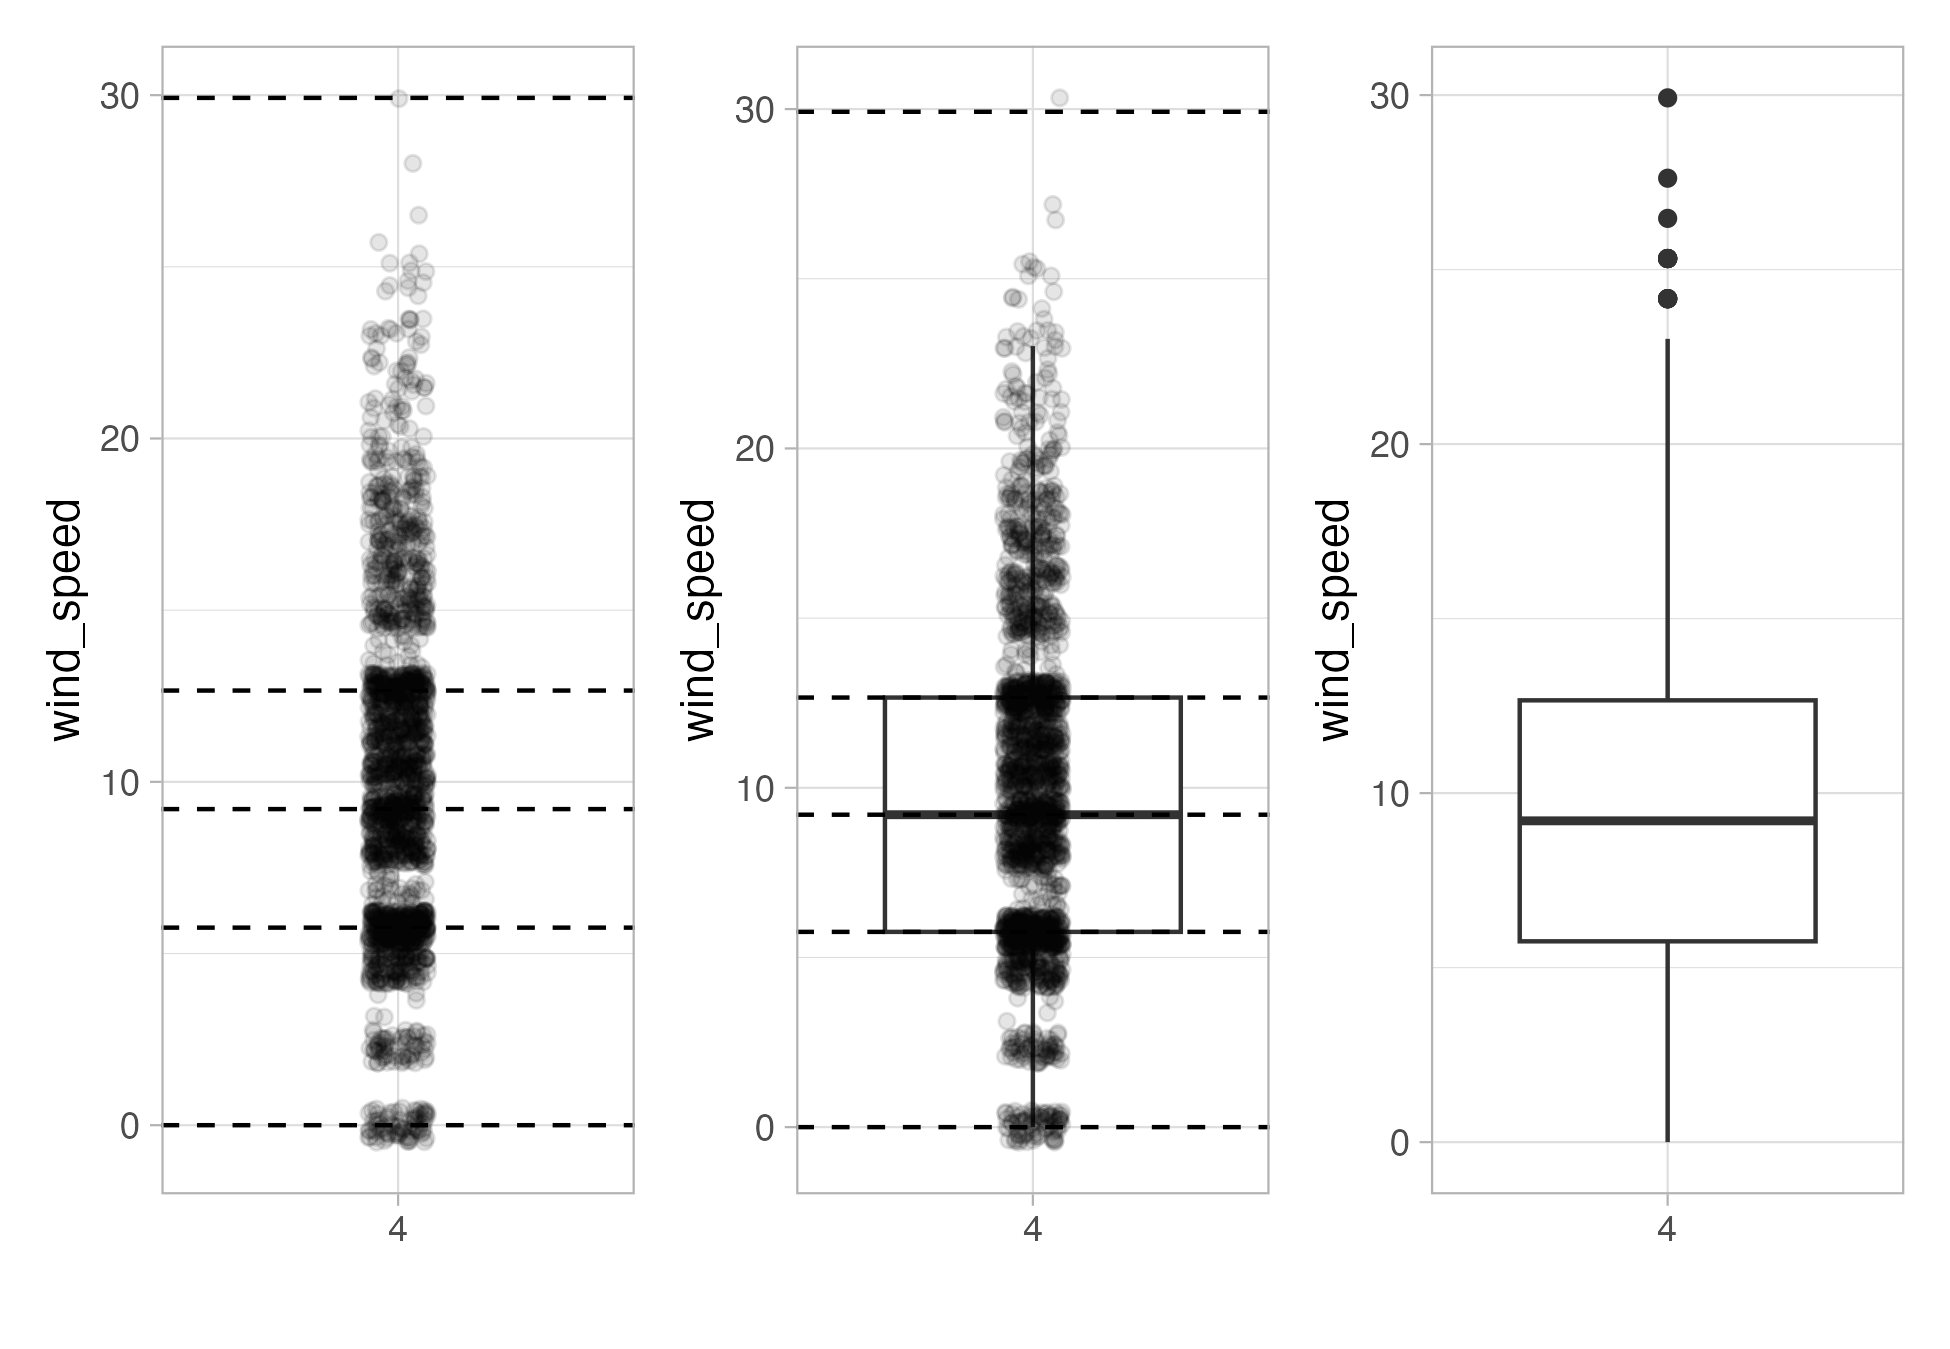
\includegraphics[width=0.7\linewidth,height=0.7\textheight]{images/patchwork_boxplot} 

}

\caption{Building up a boxplot of April wind speeds.}\label{fig:apr2}
\end{figure}

What the boxplot does is visually summarize the 2057 points by cutting the wind speed recordings into \emph{quartiles} at the dashed lines, where each quartile contains roughly 2057 \(\div\) 4 \(\approx\) 514 observations. Thus

\begin{enumerate}
\def\labelenumi{\arabic{enumi}.}
\tightlist
\item
  25\% of points fall below the bottom edge of the box, which is the first quartile of 5.8 mph. In other words, 25\% of observations were below 5.8 mph.
\item
  25\% of points fall between the bottom edge of the box and the solid middle line, which is the median of 9.2 mph. Thus, 25\% of observations were between 5.8 mph and 9.2 mph and 50\% of observations were below 9.2 mph.
\item
  25\% of points fall between the solid middle line and the top edge of the box, which is the third quartile of 12.7 mph. It follows that 25\% of observations were between 9.2 mph and 12.7 mph and 75\% of observations were below 12.7 mph.
\item
  25\% of points fall above the top edge of the box. In other words, 25\% of observations were above 12.7 mph.
\item
  The middle 50\% of points lie within the \emph{interquartile range (IQR)} \index{interquartile range (IQR)} between the first and third quartile. Thus, the IQR for this example is 12.7 - 5.8 = 6.905 mph. The interquartile range measures a numerical variable's \emph{spread}.
\end{enumerate}

Furthermore, in the rightmost plot of Figure \ref{fig:apr2}, we see the \emph{whiskers} \index{boxplots!whiskers} of the boxplot. The whiskers stick out from either end of the box all the way to the minimum and maximum observed wind speeds of 0 mph and 29.92 mph, respectively. However, the whiskers don't always extend to the smallest and largest observed values as they do here. They in fact extend no more than 1.5 \(\times\) the interquartile range from either end of the box, in this case of the April wind speeds, no more than 1.5 \(\times\) 6.905 mph = 10.357 mph from either end of the box. Any observed values outside this range get marked with points called \emph{outliers}, which are marked here, and we'll discuss further in the next section.

\subsection{\texorpdfstring{Boxplots via \texttt{geom\_boxplot}}{Boxplots via geom\_boxplot}}\label{geomboxplot}

Let's now create a side-by-side boxplot \index{boxplots!side-by-side} of hourly wind speeds split by the 12 months as we did previously with the faceted histograms. We do this by mapping the \texttt{month} variable to the x-position aesthetic, the \texttt{wind\_speed} variable to the y-position aesthetic, and by adding a \texttt{geom\_boxplot()} layer:

\begin{Shaded}
\begin{Highlighting}[]
\FunctionTok{ggplot}\NormalTok{(}\AttributeTok{data =}\NormalTok{ weather, }\AttributeTok{mapping =} \FunctionTok{aes}\NormalTok{(}\AttributeTok{x =}\NormalTok{ month, }\AttributeTok{y =}\NormalTok{ wind\_speed)) }\SpecialCharTok{+}
  \FunctionTok{geom\_boxplot}\NormalTok{()}
\end{Highlighting}
\end{Shaded}

\begin{figure}[H]

{\centering 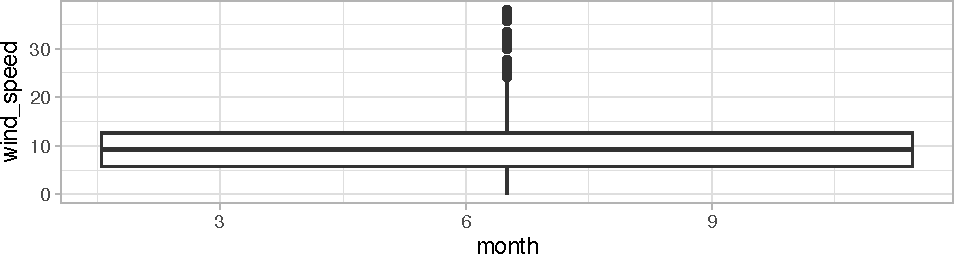
\includegraphics[width=\textwidth]{ModernDive_files/figure-latex/badbox-1} 

}

\caption{Invalid boxplot specification.}\label{fig:badbox}
\end{figure}

\begin{verbatim}
Warning message:
1: Continuous x aesthetic -- did you forget aes(group=...)? 
\end{verbatim}

Observe in Figure \ref{fig:badbox} that this plot does not provide information about wind speed separated by month. The first warning message tells us why. It says that we have a ``continuous'', or numerical variable, on the x-position aesthetic. Boxplots, however, require a categorical variable to be mapped to the x-position aesthetic.

We can convert the numerical variable \texttt{month} into a \texttt{factor} categorical variable by using the \texttt{factor()} \index{factors} function. After applying \texttt{factor(month)}, \texttt{month} goes from having just the numerical values 1, 2, \ldots, and 12 to having an associated ordering. With this ordering, \texttt{ggplot()} now knows how to work with this variable to produce the plot.

\begin{Shaded}
\begin{Highlighting}[]
\FunctionTok{ggplot}\NormalTok{(}\AttributeTok{data =}\NormalTok{ weather, }\AttributeTok{mapping =} \FunctionTok{aes}\NormalTok{(}\AttributeTok{x =} \FunctionTok{factor}\NormalTok{(month), }\AttributeTok{y =}\NormalTok{ wind\_speed)) }\SpecialCharTok{+}
  \FunctionTok{geom\_boxplot}\NormalTok{()}
\end{Highlighting}
\end{Shaded}

\begin{figure}[H]

{\centering 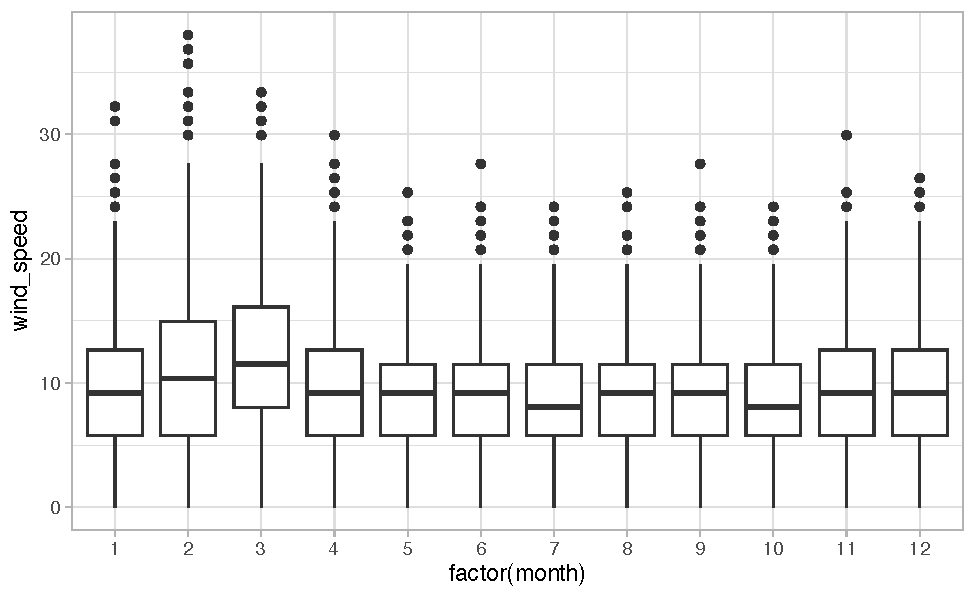
\includegraphics[width=\textwidth]{ModernDive_files/figure-latex/monthtempbox-1} 

}

\caption{Side-by-side boxplot of wind speed split by month.}\label{fig:monthtempbox}
\end{figure}

The resulting Figure \ref{fig:monthtempbox} shows 12 separate ``box and whiskers'' plots similar to the rightmost plot of Figure \ref{fig:apr2} of only April wind speeds. Thus the different boxplots are shown ``side-by-side.''

\begin{itemize}
\tightlist
\item
  The ``box'' portions of the visualization represent the 1st quartile, the median (the 2nd quartile), and the 3rd quartile.
\item
  The height of each box (the value of the 3rd quartile minus the value of the 1st quartile) is the interquartile range (IQR). It is a measure of the spread of the middle 50\% of values, with longer boxes indicating more variability.
\item
  The ``whisker'' portions of these plots extend out from the bottoms and tops of the boxes and represent points less than the 25th percentile and greater than the 75th percentiles, respectively. They're set to extend out no more than \(1.5 \times IQR\) units away from either end of the boxes. We say ``no more than'' because the ends of the whiskers have to correspond to observed wind speeds. The length of these whiskers show how the data outside the middle 50\% of values vary, with longer whiskers indicating more variability.
\item
  The dots representing values falling outside the whiskers are called \index{outliers} \emph{outliers}. These can be thought of as anomalous (``out-of-the-ordinary'') values.
\end{itemize}

It is important to keep in mind that the definition of an outlier is somewhat arbitrary and not absolute. In this case, they are defined by the length of the whiskers, which are no more than \(1.5 \times IQR\) units long for each boxplot. Looking at this side-by-side plot we can see that the months of February and March have higher median wind speeds as evidenced by the higher solid lines in the middle of the boxes. We can easily compare wind speeds across months by drawing imaginary horizontal lines across the plot. Furthermore, the heights of the 12 boxes as quantified by the interquartile ranges are informative too; they tell us about variability, or spread, of wind speeds recorded in a given month.

\begin{learncheck}
\vspace{-0.15in}

\textbf{\emph{Learning check}} \vspace{-0.1in}
\end{learncheck}

\textbf{(LC2.22)} What do the dots at the top of the plot for January correspond to? Explain what might have occurred in January to produce these points.

\textbf{(LC2.23)} Which months seem to have the highest variability in wind speed? What reasons can you give for this?

\textbf{(LC2.24)} We looked at the distribution of the numerical variable \texttt{wind\_speed} split by the numerical variable \texttt{month} that we converted using the \texttt{factor()} function in order to make a side-by-side boxplot. Why would a boxplot of \texttt{wind\_speed} split by the numerical variable \texttt{pressure} similarly converted to a categorical variable using the \texttt{factor()} not be informative?

\textbf{(LC2.25)} Boxplots provide a simple way to identify outliers. Why may outliers be easier to identify when looking at a boxplot instead of a faceted histogram?

\begin{learncheck}
\vspace{-0.25in}
\vspace{-0.25in}
\end{learncheck}

\subsection{Summary}\label{summary-3}

Side-by-side boxplots provide us with a way to compare the distribution of a numerical variable across multiple values of another variable. One can see where the median falls across the different groups by comparing the solid lines in the center of the boxes.

To study the spread of a numerical variable within one of the boxes, look at both the length of the box and also how far the whiskers extend from either end of the box. Outliers are even more easily identified when looking at a boxplot than when looking at a histogram as they are marked with distinct points.

\section{5NG\#5: Barplots}\label{geombar}

Both histograms and boxplots are tools to visualize the distribution of numerical variables. Another commonly desired task is to visualize the distribution of a categorical variable. This is a simpler task, as we are simply counting different categories within a categorical variable, also known as the \index{levels} \emph{levels} of the categorical variable. Often the best way to visualize these different counts, also known as \index{frequencies} \emph{frequencies}, is with barplots (also called barcharts).

One complication, however, is how your data is represented. Is the categorical variable of interest ``pre-counted'' or not? For example, run the following code that manually creates two data frames representing a collection of fruit: 3 apples and 2 oranges.

\begin{Shaded}
\begin{Highlighting}[]
\NormalTok{fruits }\OtherTok{\textless{}{-}} \FunctionTok{tibble}\NormalTok{(}\AttributeTok{fruit =} \FunctionTok{c}\NormalTok{(}\StringTok{"apple"}\NormalTok{, }\StringTok{"apple"}\NormalTok{, }\StringTok{"orange"}\NormalTok{, }\StringTok{"apple"}\NormalTok{, }\StringTok{"orange"}\NormalTok{))}
\NormalTok{fruits\_counted }\OtherTok{\textless{}{-}} \FunctionTok{tibble}\NormalTok{(}
  \AttributeTok{fruit =} \FunctionTok{c}\NormalTok{(}\StringTok{"apple"}\NormalTok{, }\StringTok{"orange"}\NormalTok{),}
  \AttributeTok{number =} \FunctionTok{c}\NormalTok{(}\DecValTok{3}\NormalTok{, }\DecValTok{2}\NormalTok{))}
\end{Highlighting}
\end{Shaded}

We see both the \texttt{fruits} and \texttt{fruits\_counted} data frames represent the same collection of fruit. Whereas \texttt{fruits} just lists the fruit individually\ldots{}

\begin{verbatim}
# A tibble: 5 x 1
  fruit 
  <chr> 
1 apple 
2 apple 
3 orange
4 apple 
5 orange
\end{verbatim}

\ldots{} \texttt{fruits\_counted} has a variable \texttt{count} which represent the ``pre-counted'' values of each fruit.

\begin{verbatim}
# A tibble: 2 x 2
  fruit  number
  <chr>   <dbl>
1 apple       3
2 orange      2
\end{verbatim}

Depending on how your categorical data is represented, you'll need to add a different \texttt{geom}etric layer type to your \texttt{ggplot()} to create a barplot, as we now explore.

\subsection{\texorpdfstring{Barplots via \texttt{geom\_bar} or \texttt{geom\_col}}{Barplots via geom\_bar or geom\_col}}\label{barplots-via-geom_bar-or-geom_col}

Let's generate barplots using these two different representations of the same basket of fruit: 3 apples and 2 oranges. Using the \texttt{fruits} data frame where all 5 fruits are listed individually in 5 rows, we map the \texttt{fruit} variable to the x-position aesthetic and add a \index{R packages!ggplot2!geom\_bar()} \texttt{geom\_bar()} layer:

\begin{Shaded}
\begin{Highlighting}[]
\FunctionTok{ggplot}\NormalTok{(}\AttributeTok{data =}\NormalTok{ fruits, }\AttributeTok{mapping =} \FunctionTok{aes}\NormalTok{(}\AttributeTok{x =}\NormalTok{ fruit)) }\SpecialCharTok{+}
  \FunctionTok{geom\_bar}\NormalTok{()}
\end{Highlighting}
\end{Shaded}

\begin{figure}[H]

{\centering 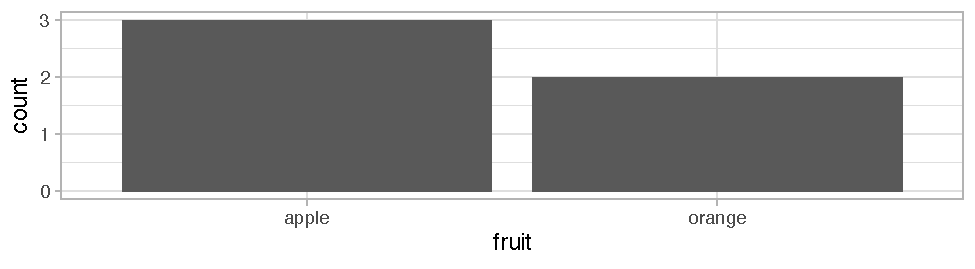
\includegraphics[width=\textwidth]{ModernDive_files/figure-latex/geombar-1} 

}

\caption{Barplot when counts are not pre-counted.}\label{fig:geombar}
\end{figure}

However, using the \texttt{fruits\_counted} data frame where the fruits have been ``pre-counted'', we once again map the \texttt{fruit} variable to the x-position aesthetic, but here we also map the \texttt{count} variable to the y-position aesthetic, and add a \index{R packages!ggplot2!geom\_col()} \texttt{geom\_col()} layer instead.

\begin{Shaded}
\begin{Highlighting}[]
\FunctionTok{ggplot}\NormalTok{(}\AttributeTok{data =}\NormalTok{ fruits\_counted, }\AttributeTok{mapping =} \FunctionTok{aes}\NormalTok{(}\AttributeTok{x =}\NormalTok{ fruit, }\AttributeTok{y =}\NormalTok{ number)) }\SpecialCharTok{+}
  \FunctionTok{geom\_col}\NormalTok{()}
\end{Highlighting}
\end{Shaded}

\begin{figure}[H]

{\centering 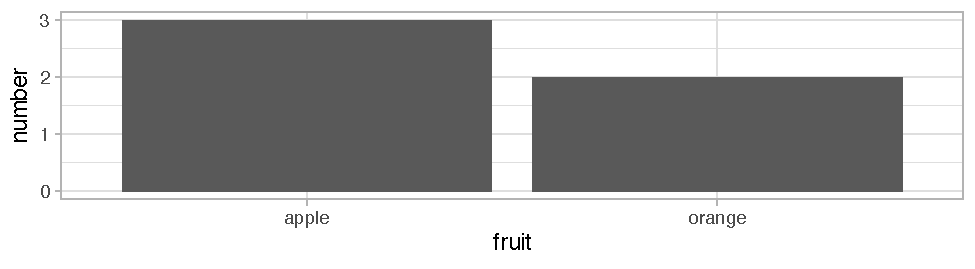
\includegraphics[width=\textwidth]{ModernDive_files/figure-latex/geomcol-1} 

}

\caption{Barplot when counts are pre-counted.}\label{fig:geomcol}
\end{figure}

Compare the barplots in Figures \ref{fig:geombar} and \ref{fig:geomcol}. They are identical because they reflect counts of the same five fruits. However, depending on how our categorical data is represented, either ``pre-counted'' or not, we must add a different \texttt{geom} layer. When the categorical variable whose distribution you want to visualize

\begin{itemize}
\tightlist
\item
  Is \emph{not} pre-counted in your data frame, we use \texttt{geom\_bar()}.
\item
  Is pre-counted in your data frame, we use \texttt{geom\_col()} with the y-position aesthetic mapped to the variable that has the counts.
\end{itemize}

Let's now go back to the \texttt{flights} data frame in the \texttt{nycflights23} package and visualize the distribution of the categorical variable \texttt{carrier}. In other words, let's visualize the number of domestic flights out of New York City each airline company flew in 2023. Recall from Subsection \ref{exploredataframes} when you first explored the \texttt{flights} data frame, you saw that each row corresponds to a flight. In other words, the \texttt{flights} data frame is more like the \texttt{fruits} data frame than the \texttt{fruits\_counted} data frame because the flights have not been pre-counted by \texttt{carrier}. Thus we should use \texttt{geom\_bar()} instead of \texttt{geom\_col()} to create a barplot. Much like a \texttt{geom\_histogram()}, there is only one variable in the \texttt{aes()} aesthetic mapping: the variable \texttt{carrier} gets mapped to the \texttt{x}-position. As a difference though, histograms have bars that touch whereas bar graphs have white space between the bars going from left to right.



\begin{Shaded}
\begin{Highlighting}[]
\FunctionTok{ggplot}\NormalTok{(}\AttributeTok{data =}\NormalTok{ flights, }\AttributeTok{mapping =} \FunctionTok{aes}\NormalTok{(}\AttributeTok{x =}\NormalTok{ carrier)) }\SpecialCharTok{+}
  \FunctionTok{geom\_bar}\NormalTok{()}
\end{Highlighting}
\end{Shaded}

\begin{figure}[H]

{\centering 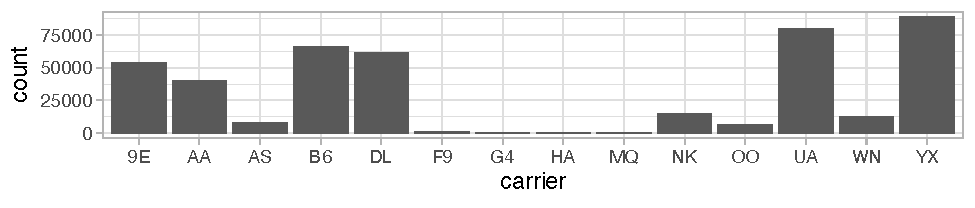
\includegraphics[width=\textwidth]{ModernDive_files/figure-latex/flightsbar-1} 

}

\caption{Number of flights departing NYC in 2023 by airline using \texttt{geom\_bar()}.}\label{fig:flightsbar}
\end{figure}

Observe in Figure \ref{fig:flightsbar} that Republic Airline (YX), United Airlines (UA), and JetBlue Airways (B6) had the most flights depart NYC in 2023. If you don't know which airlines correspond to which carrier codes, then run \texttt{View(airlines)} to see a directory of airlines. For example, AA is American Airlines Inc.~Alternatively, say you had a data frame where the number of flights for each \texttt{carrier} was pre-counted as in Table \ref{tab:flights-counted}.

\begingroup\fontsize{10}{12}\selectfont

\begin{longtable}[t]{lr}
\caption{\label{tab:flights-counted}Number of flights pre-counted for each carrier}\\
\toprule
carrier & number\\
\midrule
9E & 54141\\
AA & 40525\\
AS & 7843\\
B6 & 66169\\
DL & 61562\\
F9 & 1286\\
G4 & 671\\
HA & 366\\
MQ & 357\\
NK & 15189\\
OO & 6432\\
UA & 79641\\
WN & 12385\\
YX & 88785\\
\bottomrule
\end{longtable}
\endgroup{}

In order to create a barplot visualizing the distribution of the categorical variable \texttt{carrier} in this case, we would now use \texttt{geom\_col()} instead of \texttt{geom\_bar()}, with an additional \texttt{y\ =\ number} in the aesthetic mapping on top of the \texttt{x\ =\ carrier}. The resulting barplot would be identical to Figure \ref{fig:flightsbar}.

\begin{learncheck}
\vspace{-0.15in}

\textbf{\emph{Learning check}} \vspace{-0.1in}
\end{learncheck}

\textbf{(LC2.26)} Why are histograms inappropriate for categorical variables?

\textbf{(LC2.27)} What is the difference between histograms and barplots?

\textbf{(LC2.28)} How many Alaska Air flights departed NYC in 2023?

\textbf{(LC2.29)} What was the 7th highest airline for departed flights from NYC in 2023? How could we better present the table to get this answer quickly?

\begin{learncheck}
\vspace{-0.25in}
\vspace{-0.25in}
\end{learncheck}

\subsection{Must avoid pie charts!}\label{must-avoid-pie-charts}

One of the most common plots used to visualize the distribution of categorical data is the \index{pie charts} pie chart. While they may seem harmless enough, pie charts actually present a problem in that humans are unable to judge angles well.

As Naomi Robbins describes in her book, \emph{Creating More Effective Graphs} \citep{robbins2013}, we overestimate angles greater than 90 degrees and we underestimate angles less than 90 degrees. In other words, it is difficult for us to determine the relative size of one piece of the pie compared to another.

Let's examine the same data used in our previous barplot of the number of flights departing NYC by airline in Figure \ref{fig:flightsbar}, but this time we will use a pie chart in Figure \ref{fig:carrierpie}. Try to answer the following questions:

\begin{itemize}
\tightlist
\item
  How much smaller is the portion of the pie for Hawaiian Airlines Inc.~(\texttt{HA}) compared to United Airlines (\texttt{UA})?
\item
  What is the third largest carrier in terms of departing flights?
\item
  How many carriers have fewer flights than Delta Air Lines Inc.~(\texttt{DL})?
\end{itemize}

\begin{figure}[H]

{\centering 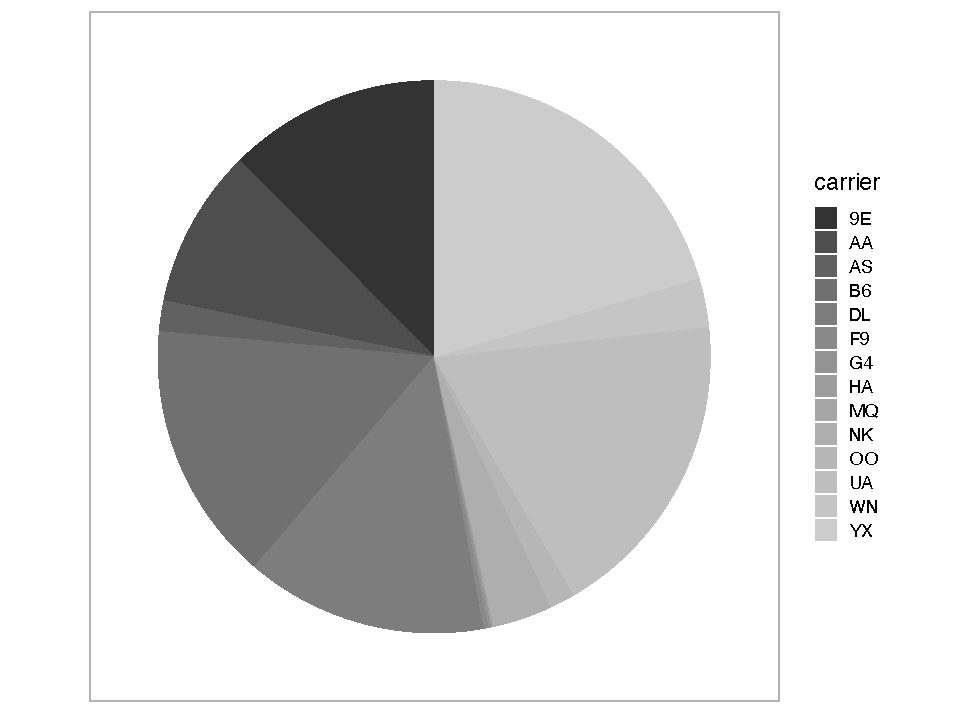
\includegraphics[width=\textwidth]{ModernDive_files/figure-latex/carrierpie-1} 

}

\caption{The dreaded pie chart.}\label{fig:carrierpie}
\end{figure}

While it is quite difficult to answer these questions when looking at the pie chart in Figure \ref{fig:carrierpie}, we can much more easily answer these questions using the barchart in Figure \ref{fig:flightsbar}. This is true since barplots present the information in a way such that comparisons between categories can be made with single horizontal lines, whereas pie charts present the information in a way such that comparisons must be made by \index{pie charts!problems with} comparing angles.

\begin{learncheck}
\vspace{-0.15in}

\textbf{\emph{Learning check}} \vspace{-0.1in}
\end{learncheck}

\textbf{(LC2.30)} Why should pie charts be avoided and replaced by barplots?

\textbf{(LC2.31)} Why do you think people continue to use pie charts?

\begin{learncheck}
\vspace{-0.25in}
\vspace{-0.25in}
\end{learncheck}

\subsection{Two categorical variables}\label{two-categ-barplot}

Barplots are a very common way to visualize the frequency of different categories, or levels, of a single categorical variable. Another use of barplots is to visualize the \emph{joint} distribution of two categorical variables at the same time. Let's examine the \emph{joint} distribution of outgoing domestic flights from NYC by \texttt{carrier} as well as \texttt{origin}, in other words, the number of flights for each \texttt{carrier} and \texttt{origin} combination. This corresponds to the number of American Airlines flights from \texttt{JFK}, the number of American Airlines flights from \texttt{LGA}, the number of American Airlines flights from \texttt{EWR}, the number of Endeavor Air flights from \texttt{JFK}, and so on. Recall the \texttt{ggplot()} code that created the barplot of \texttt{carrier} frequency in Figure \ref{fig:flightsbar}:

\begin{Shaded}
\begin{Highlighting}[]
\FunctionTok{ggplot}\NormalTok{(}\AttributeTok{data =}\NormalTok{ flights, }\AttributeTok{mapping =} \FunctionTok{aes}\NormalTok{(}\AttributeTok{x =}\NormalTok{ carrier)) }\SpecialCharTok{+} 
  \FunctionTok{geom\_bar}\NormalTok{()}
\end{Highlighting}
\end{Shaded}

We can now map the additional variable \texttt{origin} by adding a \texttt{fill\ =\ origin} inside the \texttt{aes()} aesthetic mapping.

\begin{Shaded}
\begin{Highlighting}[]
\FunctionTok{ggplot}\NormalTok{(}\AttributeTok{data =}\NormalTok{ flights, }\AttributeTok{mapping =} \FunctionTok{aes}\NormalTok{(}\AttributeTok{x =}\NormalTok{ carrier, }\AttributeTok{fill =}\NormalTok{ origin)) }\SpecialCharTok{+}
  \FunctionTok{geom\_bar}\NormalTok{()}
\end{Highlighting}
\end{Shaded}

\begin{figure}[H]

{\centering 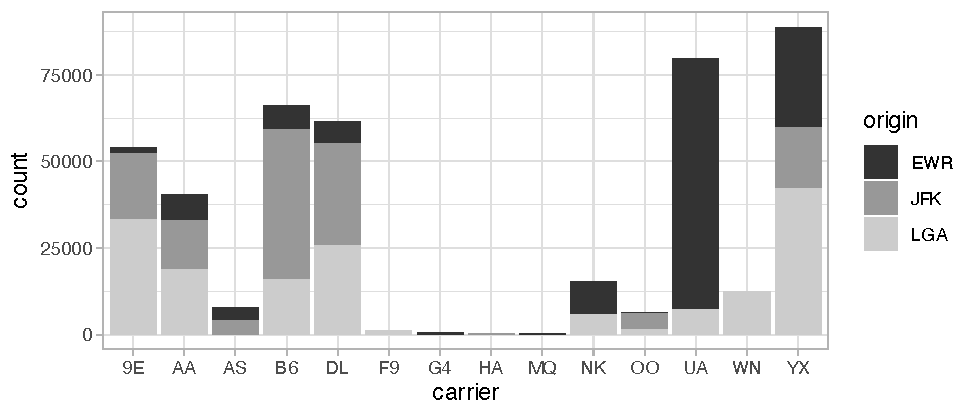
\includegraphics[width=\textwidth]{ModernDive_files/figure-latex/flights-stacked-bar-1} 

}

\caption{Stacked barplot of flight amount by carrier and origin.}\label{fig:flights-stacked-bar}
\end{figure}

Figure \ref{fig:flights-stacked-bar} is an example of a \index{barplot!stacked} \emph{stacked barplot}. While simple to make, in certain aspects it is not ideal. For example, it is difficult to compare the heights of the different colors between the bars, corresponding to comparing the number of flights from each \texttt{origin} airport between the carriers.

Before we continue, let's address some common points of confusion among new R users. First, the \texttt{fill} aesthetic corresponds to the color used to fill the bars, while the \texttt{color} aesthetic corresponds to the color of the outline of the bars. This is identical to how we added color to our histogram in Subsection \ref{geomhistogram}: we set the outline of the bars to white by setting \texttt{color\ =\ "white"} and the colors of the bars to blue steel by setting \texttt{fill\ =\ "steelblue"}. Observe in Figure \ref{fig:flights-stacked-bar-color} that mapping \texttt{origin} to \texttt{color} and not \texttt{fill} yields grey bars with different colored outlines.

\begin{Shaded}
\begin{Highlighting}[]
\FunctionTok{ggplot}\NormalTok{(}\AttributeTok{data =}\NormalTok{ flights, }\AttributeTok{mapping =} \FunctionTok{aes}\NormalTok{(}\AttributeTok{x =}\NormalTok{ carrier, }\AttributeTok{color =}\NormalTok{ origin)) }\SpecialCharTok{+}
  \FunctionTok{geom\_bar}\NormalTok{()}
\end{Highlighting}
\end{Shaded}

\begin{figure}[H]

{\centering 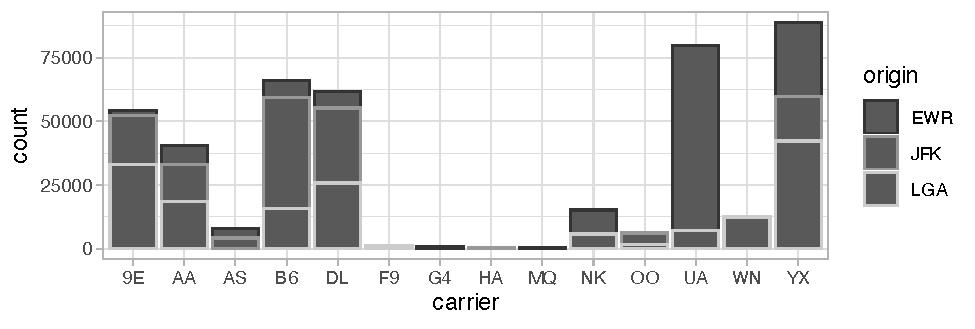
\includegraphics[width=\textwidth]{ModernDive_files/figure-latex/flights-stacked-bar-color-1} 

}

\caption{Stacked barplot with color aesthetic used instead of fill.}\label{fig:flights-stacked-bar-color}
\end{figure}

Second, note that \texttt{fill} is another aesthetic mapping much like \texttt{x}-position; thus we were careful to include it within the parentheses of the \texttt{aes()} mapping. The following code, where the \texttt{fill} aesthetic is specified outside the \texttt{aes()} mapping will yield an error. This is a fairly common error that new \texttt{ggplot} users make:

\begin{Shaded}
\begin{Highlighting}[]
\FunctionTok{ggplot}\NormalTok{(}\AttributeTok{data =}\NormalTok{ flights, }\AttributeTok{mapping =} \FunctionTok{aes}\NormalTok{(}\AttributeTok{x =}\NormalTok{ carrier), }\AttributeTok{fill =}\NormalTok{ origin) }\SpecialCharTok{+}
  \FunctionTok{geom\_bar}\NormalTok{()}
\end{Highlighting}
\end{Shaded}

An alternative to stacked barplots are \index{barplot!side-by-side} \emph{side-by-side barplots}, also known as \emph{dodged barplots}, as seen in Figure \ref{fig:flights-dodged-bar-color}. The code to create a side-by-side barplot is identical to the code to create a stacked barplot, but with a \index{R packages!ggplot2!position} \texttt{position\ =\ "dodge"} argument added to \texttt{geom\_bar()}. In other words, we are overriding the default barplot type, which is a \emph{stacked} barplot, and specifying it to be a side-by-side barplot instead.

\begin{Shaded}
\begin{Highlighting}[]
\FunctionTok{ggplot}\NormalTok{(}\AttributeTok{data =}\NormalTok{ flights, }\AttributeTok{mapping =} \FunctionTok{aes}\NormalTok{(}\AttributeTok{x =}\NormalTok{ carrier, }\AttributeTok{fill =}\NormalTok{ origin)) }\SpecialCharTok{+}
  \FunctionTok{geom\_bar}\NormalTok{(}\AttributeTok{position =} \StringTok{"dodge"}\NormalTok{)}
\end{Highlighting}
\end{Shaded}

\begin{figure}[H]

{\centering 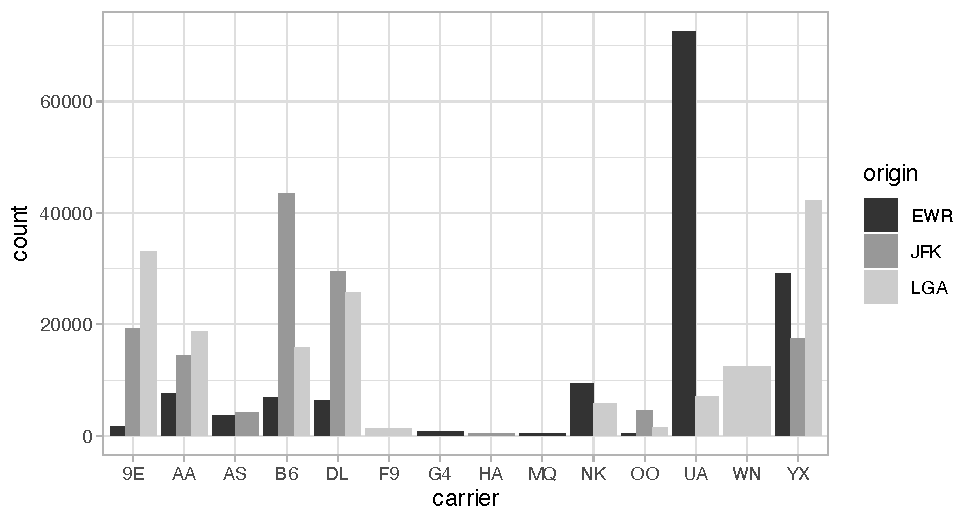
\includegraphics[width=\textwidth]{ModernDive_files/figure-latex/flights-dodged-bar-color-1} 

}

\caption{Side-by-side barplot comparing number of flights by carrier and origin.}\label{fig:flights-dodged-bar-color}
\end{figure}

Lastly, another type of barplot is a \index{barplot!faceted} \emph{faceted barplot}. Recall in Section \ref{facets} we visualized the distribution of hourly wind speeds at the 3 NYC airports \emph{split} by month using facets. We apply the same principle to our barplot visualizing the frequency of \texttt{carrier} split by \texttt{origin}: instead of mapping \texttt{origin} to \texttt{fill} we include it as the variable to create small multiples of the plot across the levels of \texttt{origin}.

\begin{Shaded}
\begin{Highlighting}[]
\FunctionTok{ggplot}\NormalTok{(}\AttributeTok{data =}\NormalTok{ flights, }\AttributeTok{mapping =} \FunctionTok{aes}\NormalTok{(}\AttributeTok{x =}\NormalTok{ carrier)) }\SpecialCharTok{+}
  \FunctionTok{geom\_bar}\NormalTok{() }\SpecialCharTok{+}
  \FunctionTok{facet\_wrap}\NormalTok{(}\SpecialCharTok{\textasciitilde{}}\NormalTok{ origin, }\AttributeTok{ncol =} \DecValTok{1}\NormalTok{)}
\end{Highlighting}
\end{Shaded}

\begin{figure}[H]

{\centering 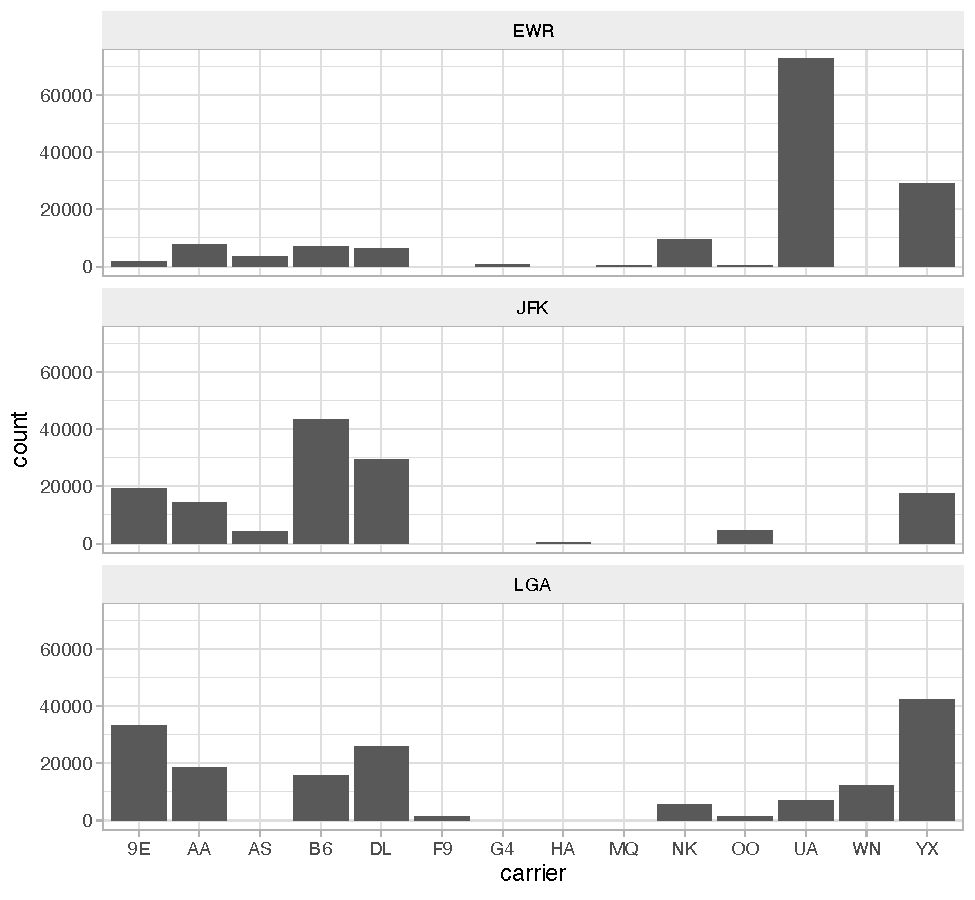
\includegraphics[width=\textwidth]{ModernDive_files/figure-latex/facet-bar-vert-1} 

}

\caption{Faceted barplot comparing the number of flights by carrier and origin.}\label{fig:facet-bar-vert}
\end{figure}

\begin{learncheck}
\vspace{-0.15in}

\textbf{\emph{Learning check}} \vspace{-0.1in}
\end{learncheck}

\textbf{(LC2.32)} What kinds of questions are not easily answered by looking at Figure \ref{fig:flights-stacked-bar}?

\textbf{(LC2.33)} What can you say, if anything, about the relationship between airline and airport in NYC in 2023 in regards to the number of departing flights?

\textbf{(LC2.34)} Why might the side-by-side barplot be preferable to a stacked barplot in this case?

\textbf{(LC2.35)} What are the disadvantages of using a dodged barplot, in general?

\textbf{(LC2.36)} Why is the faceted barplot preferred to the side-by-side and stacked barplots in this case?

\textbf{(LC2.37)} What information about the different carriers at different airports is more easily seen in the faceted barplot?

\begin{learncheck}
\vspace{-0.25in}
\vspace{-0.25in}
\end{learncheck}

\subsection{Summary}\label{summary-4}

Barplots are a common way of displaying the distribution of a categorical variable, or in other words the frequency with which the different categories (also called \emph{levels}) occur. They are easy to understand and make it easy to make comparisons across levels. Furthermore, when trying to visualize the relationship of two categorical variables, you have many options: stacked barplots, side-by-side barplots, and faceted barplots. Depending on what aspect of the relationship you are trying to emphasize, you will need to make a choice between these three types of barplots and own that choice.

\section{Conclusion}\label{data-vis-conclusion}

\subsection{Summary table}\label{summary-table}

Let's recap all five of the five named graphs (5NG) \index{five named graphs} in Table \ref{tab:viz-summary-table} summarizing their differences. Using these 5NG, you'll be able to visualize the distributions and relationships of variables contained in a wide array of datasets. This will be even more the case as we start to map more variables to more of each \texttt{geom}etric object's \texttt{aes}thetic attribute options, further unlocking the awesome power of the \texttt{ggplot2} package.

\begin{table}
\centering
\caption{\label{tab:viz-summary-table}Summary of Five Named Graphs}
\centering
\fontsize{10}{12}\selectfont
\begin{tabular}[t]{rl>{\raggedright\arraybackslash}p{1.1in}>{\raggedright\arraybackslash}p{1.2in}>{\raggedright\arraybackslash}p{1.6in}}
\toprule
  & Named graph & Shows & Geometric object & Notes\\
\midrule
1 & Scatterplot & Relationship between 2 numerical variables & geom\_point() & \\
2 & Linegraph & Relationship between 2 numerical variables & geom\_line() & Used when there is a sequential order to x-variable, e.g., time\\
3 & Histogram & Distribution of 1 numerical variable & geom\_histogram() & Facetted histograms show the distribution of 1 numerical variable split by the values of another variable\\
4 & Boxplot & Distribution of 1 numerical variable split by the values of another variable & geom\_boxplot() & \\
5 & Barplot & Distribution of 1 categorical variable & geom\_bar() when counts are not pre-counted, geom\_col() when counts are pre-counted & Stacked, side-by-side, and faceted barplots show the joint distribution of 2 categorical variables\\
\bottomrule
\end{tabular}
\end{table}

\subsection{Function argument specification}\label{function-argument-specification}

Let's go over some important points about specifying the arguments (i.e., inputs) to functions. Run the following two segments of code:

\begin{Shaded}
\begin{Highlighting}[]
\CommentTok{\# Segment 1:}
\FunctionTok{ggplot}\NormalTok{(}\AttributeTok{data =}\NormalTok{ flights, }\AttributeTok{mapping =} \FunctionTok{aes}\NormalTok{(}\AttributeTok{x =}\NormalTok{ carrier)) }\SpecialCharTok{+}
  \FunctionTok{geom\_bar}\NormalTok{()}

\CommentTok{\# Segment 2:}
\FunctionTok{ggplot}\NormalTok{(flights, }\FunctionTok{aes}\NormalTok{(}\AttributeTok{x =}\NormalTok{ carrier)) }\SpecialCharTok{+}
  \FunctionTok{geom\_bar}\NormalTok{()}
\end{Highlighting}
\end{Shaded}

You'll notice that both code segments create the same barplot, even though in the second segment we omitted the \texttt{data\ =} and \texttt{mapping\ =} code argument names. This is because the \texttt{ggplot()} function by default assumes that the \texttt{data} argument comes first and the \texttt{mapping} argument comes second. \index{functions!argument order} As long as you specify the data frame in question first and the \texttt{aes()} mapping second, you can omit the explicit statement of the argument names \texttt{data\ =} and \texttt{mapping\ =}.

Going forward for the rest of this book, all \texttt{ggplot()} code will be like the second segment: with the \texttt{data\ =} and \texttt{mapping\ =} explicit naming of the argument omitted with the default ordering of arguments respected. We'll do this for brevity's sake; it's common to see this style when reviewing other R users' code.

\subsection{Additional resources}\label{additional-resources-1}

Solutions to all \emph{Learning checks} can be found in the Appendices of the online version of the book. The Appendices start at \url{https://moderndive.com/v2/appendixa}.

An R script file of all R code used in this chapter is available at \url{https://www.moderndive.com/v2/scripts/02-visualization.R}.

If you want to further unlock the power of the \texttt{ggplot2} package for data visualization, we suggest that you check out RStudio's ``Data Visualization with ggplot2'' cheatsheet. This cheatsheet summarizes much more than what we've discussed in this chapter. In particular, it presents many more than the 5 \texttt{geom}etric objects we covered in this chapter while providing quick and easy to read visual descriptions. For all the \texttt{geom}etric objects, it also lists all the possible aesthetic attributes one can tweak. In the current version of RStudio in mid 2024, you can access this cheatsheet by going to the RStudio Menu Bar -\textgreater{} Help -\textgreater{} Cheatsheets -\textgreater{} ``Data Visualization with ggplot2.'' Alternatively, you can preview the cheat sheet by going to the ggplot2 Github page with this \href{https://github.com/rstudio/cheatsheets/blob/main/data-visualization-2.1.pdf}{link}.

\subsection{What's to come}\label{whats-to-come-3}

Recall in Figure \ref{fig:noalpha} in Section \ref{scatterplots} we visualized the relationship between departure delay and arrival delay for Envoy Air flights only, rather than \emph{all} flights. This data is saved in the \texttt{envoy\_flights} data frame from the \texttt{moderndive} package.

In reality, the \texttt{envoy\_flights} data frame is merely a subset of the \texttt{flights} data frame from the \texttt{nycflights23} package consisting of \emph{all} flights that left NYC in 2023. We created \texttt{envoy\_flights} using the following code that uses the \texttt{dplyr} package for data wrangling:

\begin{Shaded}
\begin{Highlighting}[]
\FunctionTok{library}\NormalTok{(dplyr)}

\NormalTok{envoy\_flights }\OtherTok{\textless{}{-}}\NormalTok{ flights }\SpecialCharTok{|\textgreater{}} 
  \FunctionTok{filter}\NormalTok{(carrier }\SpecialCharTok{==} \StringTok{"MQ"}\NormalTok{)}

\FunctionTok{ggplot}\NormalTok{(}\AttributeTok{data =}\NormalTok{ envoy\_flights, }\AttributeTok{mapping =} \FunctionTok{aes}\NormalTok{(}\AttributeTok{x =}\NormalTok{ dep\_delay, }\AttributeTok{y =}\NormalTok{ arr\_delay)) }\SpecialCharTok{+} 
  \FunctionTok{geom\_point}\NormalTok{()}
\end{Highlighting}
\end{Shaded}

This code takes the \texttt{flights} data frame and \texttt{filter()} it to only return the 357 rows where \texttt{carrier} is equal to \texttt{"MQ"}, Envoy Air's carrier code. (Recall from Section \ref{code} that testing for equality is specified with \index{using == instead of =} \texttt{==} and not \texttt{=}.) The code then cycles back to save the output in a new data frame called \texttt{envoy\_flights} using the \texttt{\textless{}-} \emph{assignment} operator\index{operators!assignment (<-)}.

Similarly, recall in Figure \ref{fig:hourlytemp} in Section \ref{linegraphs} we visualized hourly wind speed recordings at Newark airport only for the first 15 days of January 2023. This data is saved in the \texttt{early\_january\_2023\_weather} data frame from the \texttt{moderndive} package.

In reality, the \texttt{early\_january\_2023\_weather} data frame is merely a subset of the \texttt{weather} data frame from the \texttt{nycflights23} package consisting of \emph{all} hourly weather observations in 2023 for \emph{all} three NYC airports. We created \texttt{early\_january\_2023\_weather} using the following \texttt{dplyr} code:

\begin{Shaded}
\begin{Highlighting}[]
\NormalTok{early\_january\_2023\_weather }\OtherTok{\textless{}{-}}\NormalTok{ weather }\SpecialCharTok{|\textgreater{}} 
  \FunctionTok{filter}\NormalTok{(origin }\SpecialCharTok{==} \StringTok{"EWR"} \SpecialCharTok{\&}\NormalTok{ month }\SpecialCharTok{==} \DecValTok{1} \SpecialCharTok{\&}\NormalTok{ day }\SpecialCharTok{\textless{}=} \DecValTok{15}\NormalTok{)}

\FunctionTok{ggplot}\NormalTok{(}\AttributeTok{data =}\NormalTok{ early\_january\_2023\_weather, }\AttributeTok{mapping =} \FunctionTok{aes}\NormalTok{(}\AttributeTok{x =}\NormalTok{ time\_hour, }\AttributeTok{y =}\NormalTok{ temp)) }\SpecialCharTok{+}
  \FunctionTok{geom\_line}\NormalTok{()}
\end{Highlighting}
\end{Shaded}

This code pares down the \texttt{weather} data frame to a new data frame \texttt{early\_january\_2023\_weather} consisting of hourly wind speed recordings only for \texttt{origin\ ==\ "EWR"}, \texttt{month\ ==\ 1}, and day less than or equal to \texttt{15}.

These two code segments are a preview of Chapter \ref{wrangling} on data wrangling using the \texttt{dplyr} package. Data wrangling is the process of transforming and modifying existing data with the intent of making it more appropriate for analysis purposes. For example, these two code segments used the \texttt{filter()} function to create new data frames (\texttt{envoy\_flights} and \texttt{early\_january\_2023\_weather}) by choosing only a subset of rows of existing data frames (\texttt{flights} and \texttt{weather}). In the next chapter, we'll formally introduce the \texttt{filter()} and other data wrangling functions as well as the \emph{pipe operator} \texttt{\textbar{}\textgreater{}} which allows you to combine multiple data wrangling actions into a single sequential \emph{chain} of actions. On to Chapter \ref{wrangling} on data wrangling!

\chapter{Data Wrangling}\label{wrangling}

So far in our journey, we've seen how to look at data saved in data frames using the \texttt{glimpse()} and \texttt{View()} functions in Chapter \ref{getting-started}, and how to create data visualizations using the \texttt{ggplot2} package in Chapter \ref{viz}. In particular we studied what we term the ``five named graphs'' (5NG):

\begin{enumerate}
\def\labelenumi{\arabic{enumi}.}
\tightlist
\item
  scatterplots via \texttt{geom\_point()}
\item
  linegraphs via \texttt{geom\_line()}
\item
  boxplots via \texttt{geom\_boxplot()}
\item
  histograms via \texttt{geom\_histogram()}
\item
  barplots via \texttt{geom\_bar()} or \texttt{geom\_col()}
\end{enumerate}

We created these visualizations using the grammar of graphics, which maps variables in a data frame to the aesthetic attributes of one of the 5 \texttt{geom}etric objects. We can also control other aesthetic attributes of the geometric objects such as the size and color as seen in the Gapminder data example in Figure \ref{fig:gapminder}.

In this chapter, we'll introduce a series of functions from the \texttt{dplyr} package for data wrangling that will allow you to take a data frame and ``wrangle'' it (transform it) to suit your needs. Such functions include:

\begin{enumerate}
\def\labelenumi{\arabic{enumi}.}
\tightlist
\item
  \texttt{filter()} a data frame's existing rows to only pick out a subset of them. For example, the \texttt{alaska\_flights} data frame.
\item
  \texttt{summarize()} one or more of its columns/variables with a \emph{summary statistic}. Examples of summary statistics include the median and interquartile range of temperatures as we saw in Section \ref{boxplots} on boxplots.
\item
  \texttt{group\_by()} its rows. In other words, assign different rows to be part of the same \emph{group}. We can then combine \texttt{group\_by()} with \texttt{summarize()} to report summary statistics for each group \emph{separately}. For example, say you don't want a single overall average departure delay \texttt{dep\_delay} for all three \texttt{origin} airports combined, but rather three separate average departure delays, one computed for each of the three \texttt{origin} airports.
\item
  \texttt{mutate()} its existing columns/variables to create new ones. For example, convert hourly temperature readings from Fahrenheit to Celsius.
\item
  \texttt{arrange()} its rows. For example, sort the rows of \texttt{weather} in ascending or descending order of \texttt{temp}.
\item
  \texttt{join()} it with another data frame by matching along a ``key'' variable. In other words, merge these two data frames together.
\end{enumerate}

Notice how we used \texttt{computer\_code} font to describe the actions we want to take on our data frames. This is because the \texttt{dplyr} package for data wrangling has intuitively verb-named functions that are easy to remember.

There is a further benefit to learning to use the \texttt{dplyr} package for data wrangling: its similarity to the database querying language \href{https://en.wikipedia.org/wiki/SQL}{SQL} (pronounced ``sequel'' or spelled out as ``S'', ``Q'', ``L''). SQL (which stands for ``Structured Query Language'') is used to manage large databases quickly and efficiently and is widely used by many institutions with a lot of data. While SQL is a topic left for a book or a course on database management, keep in mind that once you learn \texttt{dplyr}, you can learn SQL easily. We'll talk more about their similarities in Subsection \ref{normal-forms}.

\subsection*{Needed packages}\label{wrangling-packages}


Let's load all the packages needed for this chapter (this assumes you've already installed them). If needed, read Section \ref{packages} for information on how to install and load R packages.

\begin{Shaded}
\begin{Highlighting}[]
\FunctionTok{library}\NormalTok{(dplyr)}
\FunctionTok{library}\NormalTok{(ggplot2)}
\FunctionTok{library}\NormalTok{(nycflights23)}
\end{Highlighting}
\end{Shaded}

\section{\texorpdfstring{The pipe operator: \texttt{\textbar{}\textgreater{}}}{The pipe operator: \textbar\textgreater{}}}\label{piping}

Before we start data wrangling, let's first introduce a nifty tool that has been a part of R since May 2021: the \index{operators!pipe} native pipe operator \texttt{\textbar{}\textgreater{}}. The pipe operator allows us to combine multiple operations in R into a single sequential \emph{chain} of actions. In modern R, the native pipe operator \texttt{\textbar{}\textgreater{}} is now the default for chaining functions, replacing the previously common tidyverse pipe (\texttt{\%\textgreater{}\%}) that was loaded with the \texttt{dplyr} package. Introduced in R 4.1.0 in May 2021, \texttt{\textbar{}\textgreater{}} offers a more intuitive and readable syntax for data wrangling and other tasks, eliminating the need for additional package dependencies.

You'll still often see R code using \texttt{\%\textgreater{}\%} in older scripts or searches online, but we'll use \texttt{\textbar{}\textgreater{}} in this book. The tidyverse pipe still works, so don't worry if you see it in other code.

Let's start with a hypothetical example. Say you would like to perform a hypothetical sequence of operations on a hypothetical data frame \texttt{x} using hypothetical functions \texttt{f()}, \texttt{g()}, and \texttt{h()}:

\begin{enumerate}
\def\labelenumi{\arabic{enumi}.}
\tightlist
\item
  Take \texttt{x} \emph{then}
\item
  Use \texttt{x} as an input to a function \texttt{f()} \emph{then}
\item
  Use the output of \texttt{f(x)} as an input to a function \texttt{g()} \emph{then}
\item
  Use the output of \texttt{g(f(x))} as an input to a function \texttt{h()}
\end{enumerate}

One way to achieve this sequence of operations is by using nesting parentheses as follows:

\begin{Shaded}
\begin{Highlighting}[]
\FunctionTok{h}\NormalTok{(}\FunctionTok{g}\NormalTok{(}\FunctionTok{f}\NormalTok{(x)))}
\end{Highlighting}
\end{Shaded}

This code isn't so hard to read since we are applying only three functions: \texttt{f()}, then \texttt{g()}, then \texttt{h()} and each of the functions is short in its name. Further, each of these functions also only has one argument. However, you can imagine that this will get progressively harder to read as the number of functions applied in your sequence increases and the arguments in each function increase as well. This is where the pipe operator \texttt{\textbar{}\textgreater{}} comes in handy. \texttt{\textbar{}\textgreater{}} takes the output of one function and then ``pipes'' it to be the input of the next function. Furthermore, a helpful trick is to read \texttt{\textbar{}\textgreater{}} as ``then'' or ``and then.'' For example, you can obtain the same output as the hypothetical sequence of functions as follows:

\begin{Shaded}
\begin{Highlighting}[]
\NormalTok{x }\SpecialCharTok{|\textgreater{}} 
  \FunctionTok{f}\NormalTok{() }\SpecialCharTok{|\textgreater{}} 
  \FunctionTok{g}\NormalTok{() }\SpecialCharTok{|\textgreater{}} 
  \FunctionTok{h}\NormalTok{()}
\end{Highlighting}
\end{Shaded}

You would read this sequence as:

\begin{enumerate}
\def\labelenumi{\arabic{enumi}.}
\tightlist
\item
  Take \texttt{x} \emph{then}
\item
  Use this output as the input to the next function \texttt{f()} \emph{then}
\item
  Use this output as the input to the next function \texttt{g()} \emph{then}
\item
  Use this output as the input to the next function \texttt{h()}
\end{enumerate}

So while both approaches achieve the same goal, the latter is much more human-readable because you can clearly read the sequence of operations line-by-line. But what are the hypothetical \texttt{x}, \texttt{f()}, \texttt{g()}, and \texttt{h()}? Throughout this chapter on data wrangling:

\begin{enumerate}
\def\labelenumi{\arabic{enumi}.}
\tightlist
\item
  The starting value \texttt{x} will be a data frame. For example, the \index{R packages!nycflights23} \texttt{flights} data frame we explored in Section \ref{nycflights}.
\item
  The sequence of functions, here \texttt{f()}, \texttt{g()}, and \texttt{h()}, will mostly be a sequence of any number of the six data wrangling verb-named functions we listed in the introduction to this chapter. For example, the \texttt{filter(carrier\ ==\ "MQ")} function and argument specified we previewed earlier.
\item
  The result will be the transformed/modified data frame that you want. In our example, we'll save the result in a new data frame by using the \texttt{\textless{}-} assignment operator with the name \texttt{alaska\_flights} via \texttt{alaska\_flights\ \textless{}-}.
\end{enumerate}

\begin{Shaded}
\begin{Highlighting}[]
\NormalTok{envoy\_flights }\OtherTok{\textless{}{-}}\NormalTok{ flights }\SpecialCharTok{|\textgreater{}} 
  \FunctionTok{filter}\NormalTok{(carrier }\SpecialCharTok{==} \StringTok{"AS"}\NormalTok{)}
\end{Highlighting}
\end{Shaded}

Much like when adding layers to a \texttt{ggplot()} using the \texttt{+} sign, you form a single \emph{chain} of data wrangling operations by combining verb-named functions into a single sequence using the pipe operator \texttt{\textbar{}\textgreater{}}. Furthermore, much like how the \texttt{+} sign has to come at the end of lines when constructing plots, the pipe operator \texttt{\textbar{}\textgreater{}} has to come at the end of lines as well.

Keep in mind, there are many more advanced data wrangling functions than just the six listed in the introduction to this chapter; you'll see some examples of these in Section \ref{other-verbs}. However, just with these six verb-named functions you'll be able to perform a broad array of data wrangling tasks for the rest of this book.

\section{\texorpdfstring{\texttt{filter} rows}{filter rows}}\label{filter}

\begin{figure}[H]

{\centering 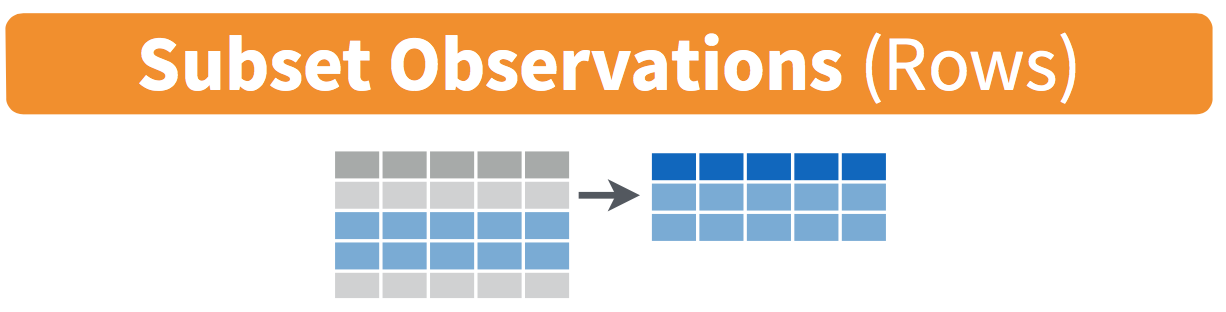
\includegraphics[width=\textwidth]{images/cheatsheets/filter} 

}

\caption{Diagram of filter() rows operation.}\label{fig:filter}
\end{figure}

The \index{R packages!dplyr!filter} \texttt{filter()} function here works much like the ``Filter'' option in Microsoft Excel; it allows you to specify criteria about the values of a variable in your dataset and then filters out only the rows that match that criteria.

We begin by focusing only on flights from New York City to Phoenix, Arizona. The \texttt{dest} destination code (or airport code) for Phoenix, Arizona is \texttt{"PHX"}. Run the following and look at the results in RStudio's spreadsheet viewer to ensure that only flights heading to Phoenix are chosen here:

\begin{Shaded}
\begin{Highlighting}[]
\NormalTok{phoenix\_flights }\OtherTok{\textless{}{-}}\NormalTok{ flights }\SpecialCharTok{|\textgreater{}} 
  \FunctionTok{filter}\NormalTok{(dest }\SpecialCharTok{==} \StringTok{"PHX"}\NormalTok{)}
\FunctionTok{View}\NormalTok{(phoenix\_flights)}
\end{Highlighting}
\end{Shaded}

Note the order of the code. First, take the \texttt{flights} data frame \texttt{flights} \emph{then} \texttt{filter()} the data frame so that only those where the \texttt{dest} equals \texttt{"PHX"} are included. We test for equality using the double equal sign \index{operators!==} \texttt{==} and not a single equal sign \texttt{=}. In other words, \texttt{filter(dest\ =\ "PHX")} will yield an error. This is a convention across many programming languages. If you are new to coding, you'll probably forget to use the double equal sign \texttt{==} a few times before you get the hang of it.

You can use other operators \index{operators} beyond just the \texttt{==} operator that tests for equality:

\begin{itemize}
\tightlist
\item
  \texttt{\textgreater{}} corresponds to ``greater than''
\item
  \texttt{\textless{}} corresponds to ``less than''
\item
  \texttt{\textgreater{}=} corresponds to ``greater than or equal to''
\item
  \texttt{\textless{}=} corresponds to ``less than or equal to''
\item
  \texttt{!=} corresponds to ``not equal to.'' The \texttt{!} is used in many programming languages to indicate ``not.''
\end{itemize}

Furthermore, you can combine multiple criteria using operators that make comparisons:

\begin{itemize}
\tightlist
\item
  \texttt{\textbar{}} corresponds to ``or''
\item
  \texttt{\&} corresponds to ``and''
\end{itemize}

To see many of these in action, let's filter \texttt{flights} for all rows that departed from JFK \emph{and} were heading to Burlington, Vermont (\texttt{"BTV"}) or Seattle, Washington (\texttt{"SEA"}) \emph{and} departed in the months of October, November, or December. Run the following:

\begin{Shaded}
\begin{Highlighting}[]
\NormalTok{btv\_sea\_flights\_fall }\OtherTok{\textless{}{-}}\NormalTok{ flights }\SpecialCharTok{|\textgreater{}} 
  \FunctionTok{filter}\NormalTok{(origin }\SpecialCharTok{==} \StringTok{"JFK"} \SpecialCharTok{\&}\NormalTok{ (dest }\SpecialCharTok{==} \StringTok{"BTV"} \SpecialCharTok{|}\NormalTok{ dest }\SpecialCharTok{==} \StringTok{"SEA"}\NormalTok{) }\SpecialCharTok{\&}\NormalTok{ month }\SpecialCharTok{\textgreater{}=} \DecValTok{10}\NormalTok{)}
\FunctionTok{View}\NormalTok{(btv\_sea\_flights\_fall)}
\end{Highlighting}
\end{Shaded}

Note that even though colloquially speaking one might say ``all flights leaving Burlington, Vermont \emph{and} Seattle, Washington,'' in terms of computer operations, we really mean ``all flights leaving Burlington, Vermont \emph{or} leaving Seattle, Washington.'' For a given row in the data, \texttt{dest} can be \texttt{"BTV"}, or \texttt{"SEA"}, or something else, but not both \texttt{"BTV"} and \texttt{"SEA"} at the same time. Furthermore, note the careful use of parentheses around \texttt{dest\ ==\ "BTV"\ \textbar{}\ dest\ ==\ "SEA"}.

We can often skip the use of \texttt{\&} and just separate our conditions with a comma. The previous code will return the identical output \texttt{btv\_sea\_flights\_fall} as the following code:

\begin{Shaded}
\begin{Highlighting}[]
\NormalTok{btv\_sea\_flights\_fall }\OtherTok{\textless{}{-}}\NormalTok{ flights }\SpecialCharTok{|\textgreater{}} 
  \FunctionTok{filter}\NormalTok{(origin }\SpecialCharTok{==} \StringTok{"JFK"}\NormalTok{, (dest }\SpecialCharTok{==} \StringTok{"BTV"} \SpecialCharTok{|}\NormalTok{ dest }\SpecialCharTok{==} \StringTok{"SEA"}\NormalTok{), month }\SpecialCharTok{\textgreater{}=} \DecValTok{10}\NormalTok{)}
\FunctionTok{View}\NormalTok{(btv\_sea\_flights\_fall)}
\end{Highlighting}
\end{Shaded}

Let's present another example that uses the \index{operators!not} \texttt{!} ``not'' operator to pick rows that \emph{don't} match a criteria. As mentioned earlier, the \texttt{!} can be read as ``not.'' Here we are filtering rows corresponding to flights that didn't go to Burlington, VT or Seattle, WA.

\begin{Shaded}
\begin{Highlighting}[]
\NormalTok{not\_BTV\_SEA }\OtherTok{\textless{}{-}}\NormalTok{ flights }\SpecialCharTok{|\textgreater{}} 
  \FunctionTok{filter}\NormalTok{(}\SpecialCharTok{!}\NormalTok{(dest }\SpecialCharTok{==} \StringTok{"BTV"} \SpecialCharTok{|}\NormalTok{ dest }\SpecialCharTok{==} \StringTok{"SEA"}\NormalTok{))}
\FunctionTok{View}\NormalTok{(not\_BTV\_SEA)}
\end{Highlighting}
\end{Shaded}

Again, note the careful use of parentheses around the \texttt{(dest\ ==\ "BTV"\ \textbar{}\ dest\ ==\ "SEA")}. If we didn't use parentheses as follows:

\begin{Shaded}
\begin{Highlighting}[]
\NormalTok{flights }\SpecialCharTok{|\textgreater{}} \FunctionTok{filter}\NormalTok{(}\SpecialCharTok{!}\NormalTok{dest }\SpecialCharTok{==} \StringTok{"BTV"} \SpecialCharTok{|}\NormalTok{ dest }\SpecialCharTok{==} \StringTok{"SEA"}\NormalTok{)}
\end{Highlighting}
\end{Shaded}

We would be returning all flights not headed to \texttt{"BTV"} \emph{or} those headed to \texttt{"SEA"}, which is an entirely different resulting data frame.

Now say we have a larger number of airports we want to filter for, say \texttt{"SEA"}, \texttt{"SFO"}, \texttt{"PHX"}, \texttt{"BTV"}, and \texttt{"BDL"}. We could continue to use the \texttt{\textbar{}} (\emph{or}) \index{operators!or} operator.

\begin{Shaded}
\begin{Highlighting}[]
\NormalTok{many\_airports }\OtherTok{\textless{}{-}}\NormalTok{ flights }\SpecialCharTok{|\textgreater{}} 
  \FunctionTok{filter}\NormalTok{(dest }\SpecialCharTok{==} \StringTok{"SEA"} \SpecialCharTok{|}\NormalTok{ dest }\SpecialCharTok{==} \StringTok{"SFO"} \SpecialCharTok{|}\NormalTok{ dest }\SpecialCharTok{==} \StringTok{"PHX"} \SpecialCharTok{|} 
\NormalTok{         dest }\SpecialCharTok{==} \StringTok{"BTV"} \SpecialCharTok{|}\NormalTok{ dest }\SpecialCharTok{==} \StringTok{"BDL"}\NormalTok{)}
\end{Highlighting}
\end{Shaded}

As we progressively include more airports, this will get unwieldy to write. A slightly shorter approach uses the \texttt{\%in\%} \index{operators!in} operator along with the \texttt{c()} function. Recall from Subsection \ref{programming-concepts} that the \texttt{c()} function ``combines'' or ``concatenates'' values into a single \emph{vector} of values. \index{vectors}

\begin{Shaded}
\begin{Highlighting}[]
\NormalTok{many\_airports }\OtherTok{\textless{}{-}}\NormalTok{ flights }\SpecialCharTok{|\textgreater{}} 
  \FunctionTok{filter}\NormalTok{(dest }\SpecialCharTok{\%in\%} \FunctionTok{c}\NormalTok{(}\StringTok{"SEA"}\NormalTok{, }\StringTok{"SFO"}\NormalTok{, }\StringTok{"PHX"}\NormalTok{, }\StringTok{"BTV"}\NormalTok{, }\StringTok{"BDL"}\NormalTok{))}
\FunctionTok{View}\NormalTok{(many\_airports)}
\end{Highlighting}
\end{Shaded}

What this code is doing is filtering \texttt{flights} for all flights where \texttt{dest} is in the vector of airports \texttt{c("BTV",\ "SEA",\ "PHX",\ "SFO",\ "BDL")}. Both outputs of \texttt{many\_airports} are the same, but as you can see the latter takes much less energy to code. The \texttt{\%in\%} operator is useful for looking for matches commonly in one vector/variable compared to another.

As a final note, we recommend that \texttt{filter()} should often be among the first verbs you consider applying to your data. This cleans your dataset to only those rows you care about, or put differently, it narrows down the scope of your data frame to just the observations you care about.

\begin{learncheck}
\vspace{-0.15in}

\textbf{\emph{Learning check}} \vspace{-0.1in}
\end{learncheck}

\textbf{(LC3.1)} What's another way of using the ``not'' operator \texttt{!} to filter only the rows that are not going to Burlington, VT nor Seattle, WA in the \texttt{flights} data frame? Test this out using the previous code.

\begin{learncheck}
\vspace{-0.25in}
\vspace{-0.25in}
\end{learncheck}

\section{\texorpdfstring{\texttt{summarize} variables}{summarize variables}}\label{summarize}

The next common task when working with data frames is to compute \emph{summary statistics}. \index{summary statistics}Summary statistics are single numerical values that summarize a large number of values. Commonly known examples of summary statistics include the mean (also called the average) and the median (the middle value). Other examples of summary statistics that might not immediately come to mind include the \emph{sum}, the smallest value also called the \emph{minimum}, the largest value also called the \emph{maximum}, and the \emph{standard deviation}.

Let's calculate two summary statistics of the \texttt{wind\_speed} temperature variable in the \texttt{weather} data frame: the mean and standard deviation (recall from Section \ref{nycflights} that the \texttt{weather} data frame is included in the \texttt{nycflights23} package). To compute these summary statistics, we need the \texttt{mean()} and \texttt{sd()} \emph{summary functions} in R. Summary functions in R take in many values and return a single value, as illustrated in Figure \ref{fig:summary-function}.

\begin{figure}[H]

{\centering 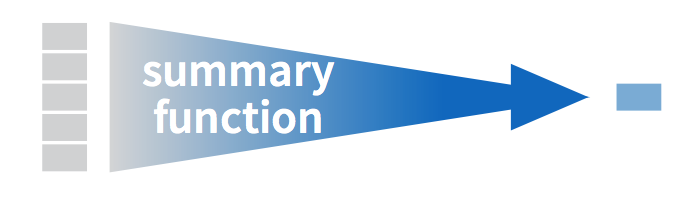
\includegraphics[width=0.8\linewidth,height=0.8\textheight]{images/cheatsheets/summary} 

}

\caption{Diagram illustrating a summary function in R.}\label{fig:summary-function}
\end{figure}

More precisely, we'll use the \texttt{mean()} and \texttt{sd()} summary functions within the \texttt{summarize()} \index{R packages!dplyr!summarize()} function from the \texttt{dplyr} package. Note you can also use the British English spelling of \texttt{summarise()}. As shown in Figure \ref{fig:sum1}, the \texttt{summarize()} function takes in a data frame and returns a data frame with only one row corresponding to the summary statistics.

\begin{figure}[H]

{\centering 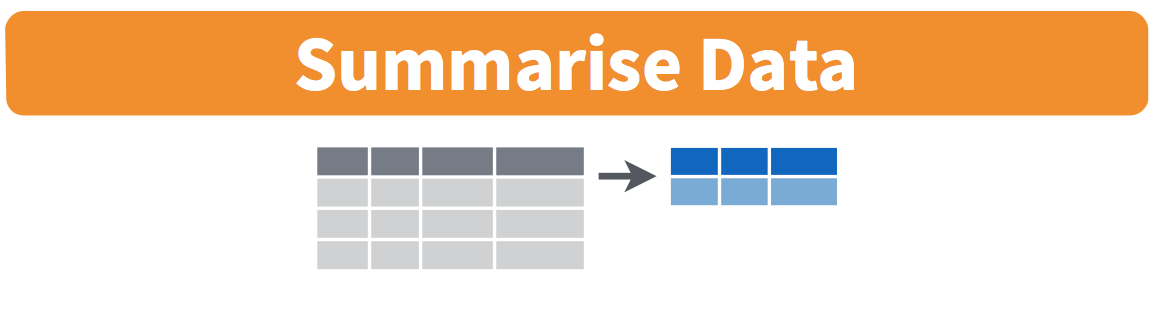
\includegraphics[width=0.8\linewidth,height=0.8\textheight]{images/cheatsheets/summarize1} 

}

\caption{Diagram of summarize() rows.}\label{fig:sum1}
\end{figure}

We'll save the results in a new data frame called \texttt{summary\_windspeed} that will have two columns/variables: the \texttt{mean} and the \texttt{std\_dev}:

\begin{Shaded}
\begin{Highlighting}[]
\NormalTok{summary\_windspeed }\OtherTok{\textless{}{-}}\NormalTok{ weather }\SpecialCharTok{|\textgreater{}} 
  \FunctionTok{summarize}\NormalTok{(}\AttributeTok{mean =} \FunctionTok{mean}\NormalTok{(wind\_speed), }\AttributeTok{std\_dev =} \FunctionTok{sd}\NormalTok{(wind\_speed))}
\NormalTok{summary\_windspeed}
\end{Highlighting}
\end{Shaded}

\begin{verbatim}
# A tibble: 1 x 2
   mean std_dev
  <dbl>   <dbl>
1    NA      NA
\end{verbatim}

Why are the values returned \texttt{NA}? \texttt{NA} is how R encodes \emph{missing values} \index{missing values} where \texttt{NA} indicates ``not available'' or ``not applicable.'' If a value for a particular row and a particular column does not exist, \texttt{NA} is stored instead. Values can be missing for many reasons. Perhaps the data was collected but someone forgot to enter it? Perhaps the data was not collected at all because it was too difficult to do so? Perhaps there was an erroneous value that someone entered that has been corrected to read as missing? You'll often encounter issues with missing values when working with real data.

Going back to our \texttt{summary\_windspeed} output, by default any time you try to calculate a summary statistic of a variable that has one or more \texttt{NA} missing values in R, \texttt{NA} is returned. To work around this fact, you can set the \texttt{na.rm} argument to \texttt{TRUE}, where \texttt{rm} is short for ``remove''; this will ignore any \texttt{NA} missing values and only return the summary value for all non-missing values.

The code that follows computes the mean and standard deviation of all non-missing values of \texttt{temp}:

\begin{Shaded}
\begin{Highlighting}[]
\NormalTok{summary\_windspeed }\OtherTok{\textless{}{-}}\NormalTok{ weather }\SpecialCharTok{|\textgreater{}} 
  \FunctionTok{summarize}\NormalTok{(}\AttributeTok{mean =} \FunctionTok{mean}\NormalTok{(wind\_speed, }\AttributeTok{na.rm =} \ConstantTok{TRUE}\NormalTok{), }
            \AttributeTok{std\_dev =} \FunctionTok{sd}\NormalTok{(wind\_speed, }\AttributeTok{na.rm =} \ConstantTok{TRUE}\NormalTok{))}
\NormalTok{summary\_windspeed}
\end{Highlighting}
\end{Shaded}

\begin{verbatim}
# A tibble: 1 x 2
   mean std_dev
  <dbl>   <dbl>
1  9.44    5.26
\end{verbatim}

Notice how the \texttt{na.rm\ =\ TRUE} \index{functions!na.rm argument} are used as arguments to the \texttt{mean()} \index{mean()} and \texttt{sd()} \index{sd()} summary functions individually, and not to the \texttt{summarize()} function.

However, one needs to be cautious whenever ignoring missing values as we've just done. In the upcoming \emph{Learning checks} questions, we'll consider the possible ramifications of blindly sweeping rows with missing values ``under the rug.'' This is in fact why the \texttt{na.rm} argument to any summary statistic function in R is set to \texttt{FALSE} by default. In other words, R does not ignore rows with missing values by default. R is alerting you to the presence of missing data and you should be mindful of this missingness and any potential causes of this missingness throughout your analysis.

What are other summary functions we can use inside the \texttt{summarize()} verb to compute summary statistics? As seen in the diagram in Figure \ref{fig:summary-function}, you can use any function in R that takes many values and returns just one. Here are just a few:

\begin{itemize}
\tightlist
\item
  \texttt{mean()}: the average
\item
  \texttt{sd()}: the standard deviation, which is a measure of spread
\item
  \texttt{min()} and \texttt{max()}: the minimum and maximum values, respectively
\item
  \texttt{IQR()}: interquartile range
\item
  \texttt{sum()}: the total amount when adding multiple numbers
\item
  \texttt{n()}: a count of the number of rows in each group. This particular summary function will make more sense when \texttt{group\_by()} is covered in Section \ref{groupby}.
\end{itemize}

\begin{learncheck}
\vspace{-0.15in}

\textbf{\emph{Learning check}} \vspace{-0.1in}
\end{learncheck}

\textbf{(LC3.2)} Say a doctor is studying the effect of smoking on lung cancer for a large number of patients who have records measured at five-year intervals. She notices that a large number of patients have missing data points because the patient has died, so she chooses to ignore these patients in her analysis. What is wrong with this doctor's approach?

\textbf{(LC3.3)} Modify the earlier \texttt{summarize()} function code that creates the \texttt{summary\_windspeed} data frame to also use the \texttt{n()} summary function: \texttt{summarize(...\ ,\ count\ =\ n())}. What does the returned value correspond to?

\textbf{(LC3.4)} Why doesn't the following code work? Run the code line-by-line instead of all at once, and then look at the data. In other words, select and then run \texttt{summary\_windspeed\ \textless{}-\ weather\ \textbar{}\textgreater{}\ summarize(mean\ =\ mean(wind\_speed,\ na.rm\ =\ TRUE))} first.

\begin{Shaded}
\begin{Highlighting}[]
\NormalTok{summary\_windspeed }\OtherTok{\textless{}{-}}\NormalTok{ weather }\SpecialCharTok{|\textgreater{}}   
  \FunctionTok{summarize}\NormalTok{(}\AttributeTok{mean =} \FunctionTok{mean}\NormalTok{(wind\_speed, }\AttributeTok{na.rm =} \ConstantTok{TRUE}\NormalTok{)) }\SpecialCharTok{|\textgreater{}} 
  \FunctionTok{summarize}\NormalTok{(}\AttributeTok{std\_dev =} \FunctionTok{sd}\NormalTok{(wind\_speed, }\AttributeTok{na.rm =} \ConstantTok{TRUE}\NormalTok{))}
\end{Highlighting}
\end{Shaded}

\begin{learncheck}
\vspace{-0.25in}
\vspace{-0.25in}
\end{learncheck}

\section{\texorpdfstring{\texttt{group\_by} rows}{group\_by rows}}\label{groupby}



\begin{figure}[H]

{\centering 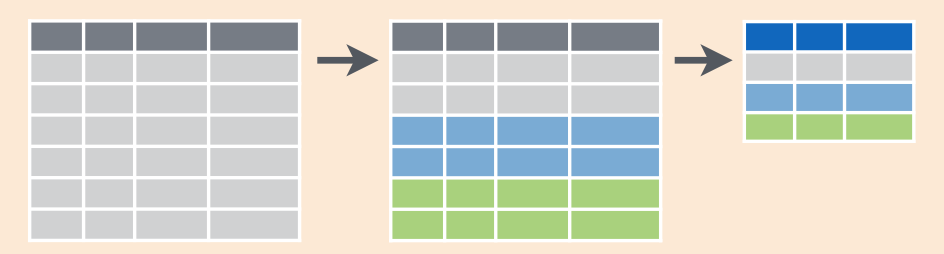
\includegraphics[width=\textwidth]{images/cheatsheets/group_summary} 

}

\caption{Diagram of group\_by() and summarize().}\label{fig:groupsummarize}
\end{figure}

We can modify our code above to look at the average wind speed and its spread instead of wind speed too, keeping the \texttt{na.rm\ =\ TRUE} set just in case any missing values are stored in the \texttt{temp} column:

\begin{Shaded}
\begin{Highlighting}[]
\NormalTok{summary\_temp }\OtherTok{\textless{}{-}}\NormalTok{ weather }\SpecialCharTok{|\textgreater{}} 
  \FunctionTok{summarize}\NormalTok{(}\AttributeTok{mean =} \FunctionTok{mean}\NormalTok{(wind\_speed, }\AttributeTok{na.rm =} \ConstantTok{TRUE}\NormalTok{), }
            \AttributeTok{std\_dev =} \FunctionTok{sd}\NormalTok{(wind\_speed, }\AttributeTok{na.rm =} \ConstantTok{TRUE}\NormalTok{))}
\NormalTok{summary\_temp}
\end{Highlighting}
\end{Shaded}

\begin{verbatim}
# A tibble: 1 x 2
   mean std_dev
  <dbl>   <dbl>
1  9.44    5.26
\end{verbatim}

Say instead of a single mean wind speed for the whole year, we would like 12 mean temperatures, one for each of the 12 months separately. In other words, we would like to compute the mean wind speed split by month. We can do this by ``grouping'' temperature observations by the values of another variable, in this case by the 12 values of the variable \texttt{month}:

\begin{Shaded}
\begin{Highlighting}[]
\NormalTok{summary\_monthly\_windspeed }\OtherTok{\textless{}{-}}\NormalTok{ weather }\SpecialCharTok{|\textgreater{}} 
  \FunctionTok{group\_by}\NormalTok{(month) }\SpecialCharTok{|\textgreater{}} 
  \FunctionTok{summarize}\NormalTok{(}\AttributeTok{mean =} \FunctionTok{mean}\NormalTok{(wind\_speed, }\AttributeTok{na.rm =} \ConstantTok{TRUE}\NormalTok{), }
            \AttributeTok{std\_dev =} \FunctionTok{sd}\NormalTok{(wind\_speed, }\AttributeTok{na.rm =} \ConstantTok{TRUE}\NormalTok{))}
\NormalTok{summary\_monthly\_windspeed}
\end{Highlighting}
\end{Shaded}

\begin{verbatim}
# A tibble: 12 x 3
   month  mean std_dev
   <int> <dbl>   <dbl>
 1     1 10.3     6.01
 2     2 10.9     6.57
 3     3 12.3     6.33
 4     4 10.0     5.03
 5     5  8.89    4.46
 6     6  8.53    4.43
 7     7  7.98    4.35
 8     8  8.85    4.34
 9     9  8.92    4.66
10    10  8.23    4.69
11    11  9.50    4.84
12    12  8.77    5.02
\end{verbatim}

This code is identical to the previous code that created \texttt{summary\_windspeed}, but with an extra \texttt{group\_by(month)} added before the \texttt{summarize()}. Grouping the \texttt{weather} dataset by \texttt{month} and then applying the \texttt{summarize()} functions yields a data frame that displays the mean and standard deviation wind speed split by the 12 months of the year.

It is important to note that the \index{R packages!dplyr!group\_by()} \texttt{group\_by()} function doesn't change data frames by itself. Rather it changes the \emph{meta-data}\index{meta-data}, or data about the data, specifically the grouping structure. Only after applying the \texttt{summarize()} function does the data frame change.

As another example, consider the \index{R packages!ggplot2!diamonds} \texttt{diamonds} data frame included in the \texttt{ggplot2} package:

\begin{Shaded}
\begin{Highlighting}[]
\NormalTok{diamonds}
\end{Highlighting}
\end{Shaded}

\begin{verbatim}
# A tibble: 53,940 x 10
   carat cut       color clarity depth table price     x     y     z
   <dbl> <ord>     <ord> <ord>   <dbl> <dbl> <int> <dbl> <dbl> <dbl>
 1  0.23 Ideal     E     SI2      61.5    55   326  3.95  3.98  2.43
 2  0.21 Premium   E     SI1      59.8    61   326  3.89  3.84  2.31
 3  0.23 Good      E     VS1      56.9    65   327  4.05  4.07  2.31
 4  0.29 Premium   I     VS2      62.4    58   334  4.2   4.23  2.63
 5  0.31 Good      J     SI2      63.3    58   335  4.34  4.35  2.75
 6  0.24 Very Good J     VVS2     62.8    57   336  3.94  3.96  2.48
 7  0.24 Very Good I     VVS1     62.3    57   336  3.95  3.98  2.47
 8  0.26 Very Good H     SI1      61.9    55   337  4.07  4.11  2.53
 9  0.22 Fair      E     VS2      65.1    61   337  3.87  3.78  2.49
10  0.23 Very Good H     VS1      59.4    61   338  4     4.05  2.39
# i 53,930 more rows
\end{verbatim}

Observe that the first line of the output reads \texttt{\#\ A\ tibble:\ 53,940\ x\ 10}. This is an example of meta-data, in this case the number of observations/rows and variables/columns in \texttt{diamonds}. The actual data itself are the subsequent table of values. Now let's pipe the \texttt{diamonds} data frame into \texttt{group\_by(cut)}:

\begin{Shaded}
\begin{Highlighting}[]
\NormalTok{diamonds }\SpecialCharTok{|\textgreater{}} 
  \FunctionTok{group\_by}\NormalTok{(cut)}
\end{Highlighting}
\end{Shaded}

\begin{verbatim}
# A tibble: 53,940 x 10
# Groups:   cut [5]
   carat cut       color clarity depth table price     x     y     z
   <dbl> <ord>     <ord> <ord>   <dbl> <dbl> <int> <dbl> <dbl> <dbl>
 1  0.23 Ideal     E     SI2      61.5    55   326  3.95  3.98  2.43
 2  0.21 Premium   E     SI1      59.8    61   326  3.89  3.84  2.31
 3  0.23 Good      E     VS1      56.9    65   327  4.05  4.07  2.31
 4  0.29 Premium   I     VS2      62.4    58   334  4.2   4.23  2.63
 5  0.31 Good      J     SI2      63.3    58   335  4.34  4.35  2.75
 6  0.24 Very Good J     VVS2     62.8    57   336  3.94  3.96  2.48
 7  0.24 Very Good I     VVS1     62.3    57   336  3.95  3.98  2.47
 8  0.26 Very Good H     SI1      61.9    55   337  4.07  4.11  2.53
 9  0.22 Fair      E     VS2      65.1    61   337  3.87  3.78  2.49
10  0.23 Very Good H     VS1      59.4    61   338  4     4.05  2.39
# i 53,930 more rows
\end{verbatim}

Observe that now there is additional meta-data: \texttt{\#\ Groups:\ cut\ {[}5{]}} indicating that the grouping structure meta-data has been set based on the 5 possible levels of the categorical variable \texttt{cut}: \texttt{"Fair"}, \texttt{"Good"}, \texttt{"Very\ Good"}, \texttt{"Premium"}, and \texttt{"Ideal"}. On the other hand, observe that the data has not changed: it is still a table of 53,940 \(\times\) 10 values. Only by combining a \texttt{group\_by()} with another data wrangling operation, in this case \texttt{summarize()}, will the data actually be transformed.

\begin{Shaded}
\begin{Highlighting}[]
\NormalTok{diamonds }\SpecialCharTok{|\textgreater{}} 
  \FunctionTok{group\_by}\NormalTok{(cut) }\SpecialCharTok{|\textgreater{}} 
  \FunctionTok{summarize}\NormalTok{(}\AttributeTok{avg\_price =} \FunctionTok{mean}\NormalTok{(price))}
\end{Highlighting}
\end{Shaded}

\begin{verbatim}
# A tibble: 5 x 2
  cut       avg_price
  <ord>         <dbl>
1 Fair          4359.
2 Good          3929.
3 Very Good     3982.
4 Premium       4584.
5 Ideal         3458.
\end{verbatim}

If you would like to remove this grouping structure meta-data, we can pipe the resulting data frame into the \index{R packages!dplyr!ungroup()} \texttt{ungroup()} function:

\begin{Shaded}
\begin{Highlighting}[]
\NormalTok{diamonds }\SpecialCharTok{|\textgreater{}} 
  \FunctionTok{group\_by}\NormalTok{(cut) }\SpecialCharTok{|\textgreater{}} 
  \FunctionTok{ungroup}\NormalTok{()}
\end{Highlighting}
\end{Shaded}

\begin{verbatim}
# A tibble: 53,940 x 10
   carat cut       color clarity depth table price     x     y     z
   <dbl> <ord>     <ord> <ord>   <dbl> <dbl> <int> <dbl> <dbl> <dbl>
 1  0.23 Ideal     E     SI2      61.5    55   326  3.95  3.98  2.43
 2  0.21 Premium   E     SI1      59.8    61   326  3.89  3.84  2.31
 3  0.23 Good      E     VS1      56.9    65   327  4.05  4.07  2.31
 4  0.29 Premium   I     VS2      62.4    58   334  4.2   4.23  2.63
 5  0.31 Good      J     SI2      63.3    58   335  4.34  4.35  2.75
 6  0.24 Very Good J     VVS2     62.8    57   336  3.94  3.96  2.48
 7  0.24 Very Good I     VVS1     62.3    57   336  3.95  3.98  2.47
 8  0.26 Very Good H     SI1      61.9    55   337  4.07  4.11  2.53
 9  0.22 Fair      E     VS2      65.1    61   337  3.87  3.78  2.49
10  0.23 Very Good H     VS1      59.4    61   338  4     4.05  2.39
# i 53,930 more rows
\end{verbatim}

Observe how the \texttt{\#\ Groups:\ cut\ {[}5{]}} meta-data is no longer present.

Let's now revisit the \texttt{n()} \index{R packages!dplyr!n()} counting summary function we briefly introduced previously. Recall that the \texttt{n()} function counts rows. This is opposed to the \texttt{sum()} summary function that returns the sum of a numerical variable. For example, suppose we'd like to count how many flights departed each of the three airports in New York City:

\begin{Shaded}
\begin{Highlighting}[]
\NormalTok{by\_origin }\OtherTok{\textless{}{-}}\NormalTok{ flights }\SpecialCharTok{|\textgreater{}} 
  \FunctionTok{group\_by}\NormalTok{(origin) }\SpecialCharTok{|\textgreater{}} 
  \FunctionTok{summarize}\NormalTok{(}\AttributeTok{count =} \FunctionTok{n}\NormalTok{())}
\NormalTok{by\_origin}
\end{Highlighting}
\end{Shaded}

\begin{verbatim}
# A tibble: 3 x 2
  origin  count
  <chr>   <int>
1 EWR    138578
2 JFK    133048
3 LGA    163726
\end{verbatim}

We see that LaGuardia (\texttt{"LGA"}) had the most flights departing in 2023 followed by Newark (\texttt{"EWR"}) and lastly by \texttt{"JFK"}. Note there is a subtle but important difference between \texttt{sum()} and \texttt{n()}; while \texttt{sum()} returns the sum of a numerical variable, \texttt{n()} returns a count of the number of rows/observations.

\subsubsection*{Grouping by more than one variable}\label{grouping-by-more-than-one-variable}


You are not limited to grouping by one variable. Say you want to know the number of flights leaving each of the three New York City airports \emph{for each month}. We can also group by a second variable \texttt{month} using \texttt{group\_by(origin,\ month)}:

\begin{Shaded}
\begin{Highlighting}[]
\NormalTok{by\_origin\_monthly }\OtherTok{\textless{}{-}}\NormalTok{ flights }\SpecialCharTok{|\textgreater{}} 
  \FunctionTok{group\_by}\NormalTok{(origin, month) }\SpecialCharTok{|\textgreater{}} 
  \FunctionTok{summarize}\NormalTok{(}\AttributeTok{count =} \FunctionTok{n}\NormalTok{())}
\end{Highlighting}
\end{Shaded}

\begin{verbatim}
`summarise()` has grouped output by 'origin'. You can override using the
`.groups` argument.
\end{verbatim}

Note that an additional message appears here specifying the grouping done. The \texttt{.groups} argument to \texttt{summarize()} has four options: \texttt{drop\_last}, \texttt{drop}, \texttt{keep}, and \texttt{rowwise}:

\begin{itemize}
\tightlist
\item
  \texttt{drop\_last} drops the last grouping variable,
\item
  \texttt{drop} drops all grouping variables,
\item
  \texttt{keep} keeps all grouping variables, and
\item
  \texttt{rowwise} turns each row into a group.
\end{itemize}

In most circumstances, the default is \texttt{drop\_last} which drops the last grouping variable. The message is informing us that the default behavior is to drop the last grouping variable, which in this case is \texttt{month}.

\begin{Shaded}
\begin{Highlighting}[]
\NormalTok{by\_origin\_monthly}
\end{Highlighting}
\end{Shaded}

\begin{verbatim}
# A tibble: 36 x 3
# Groups:   origin [3]
   origin month count
   <chr>  <int> <int>
 1 EWR        1 11623
 2 EWR        2 10991
 3 EWR        3 12593
 4 EWR        4 12022
 5 EWR        5 12371
 6 EWR        6 11339
 7 EWR        7 11646
 8 EWR        8 11561
 9 EWR        9 11373
10 EWR       10 11805
# i 26 more rows
\end{verbatim}

Observe that there are 36 rows to \texttt{by\_origin\_monthly} because there are 12 months for 3 airports (\texttt{EWR}, \texttt{JFK}, and \texttt{LGA}). Why do we \texttt{group\_by(origin,\ month)} and not \texttt{group\_by(origin)} and then \texttt{group\_by(month)}? Let's investigate:

\begin{Shaded}
\begin{Highlighting}[]
\NormalTok{by\_origin\_monthly\_incorrect }\OtherTok{\textless{}{-}}\NormalTok{ flights }\SpecialCharTok{|\textgreater{}} 
  \FunctionTok{group\_by}\NormalTok{(origin) }\SpecialCharTok{|\textgreater{}} 
  \FunctionTok{group\_by}\NormalTok{(month) }\SpecialCharTok{|\textgreater{}} 
  \FunctionTok{summarize}\NormalTok{(}\AttributeTok{count =} \FunctionTok{n}\NormalTok{())}
\NormalTok{by\_origin\_monthly\_incorrect}
\end{Highlighting}
\end{Shaded}

\begin{verbatim}
# A tibble: 12 x 2
   month count
   <int> <int>
 1     1 36020
 2     2 34761
 3     3 39514
 4     4 37476
 5     5 38710
 6     6 35921
 7     7 36211
 8     8 36765
 9     9 35505
10    10 36586
11    11 34521
12    12 33362
\end{verbatim}

What happened here is that the second \texttt{group\_by(month)} overwrote the grouping structure meta-data of the earlier \texttt{group\_by(origin)}, so that in the end we are only grouping by \texttt{month}. The lesson here is if you want to \texttt{group\_by()} two or more variables, you should include all the variables at the same time in the same \texttt{group\_by()} adding a comma between the variable names.

\begin{learncheck}
\vspace{-0.15in}

\textbf{\emph{Learning check}} \vspace{-0.1in}
\end{learncheck}

\textbf{(LC3.5)} Recall from Chapter \ref{viz} when we looked at wind speeds by months in NYC. What does the standard deviation column in the \texttt{summary\_monthly\_temp} data frame tell us about temperatures in NYC throughout the year?

\textbf{(LC3.6)} What code would be required to get the mean and standard deviation wind speed for each day in 2023 for NYC?

\textbf{(LC3.7)} Recreate \texttt{by\_monthly\_origin}, but instead of grouping via \texttt{group\_by(origin,\ month)}, group variables in a different order \texttt{group\_by(month,\ origin)}. What differs in the resulting dataset?

\textbf{(LC3.8)} How could we identify how many flights left each of the three airports for each \texttt{carrier}?

\textbf{(LC3.9)} How does the \texttt{filter()} operation differ from a \texttt{group\_by()} followed by a \texttt{summarize()}?

\begin{learncheck}
\vspace{-0.25in}
\vspace{-0.25in}
\end{learncheck}

\section{\texorpdfstring{\texttt{mutate} existing variables}{mutate existing variables}}\label{mutate}

\begin{figure}[H]

{\centering 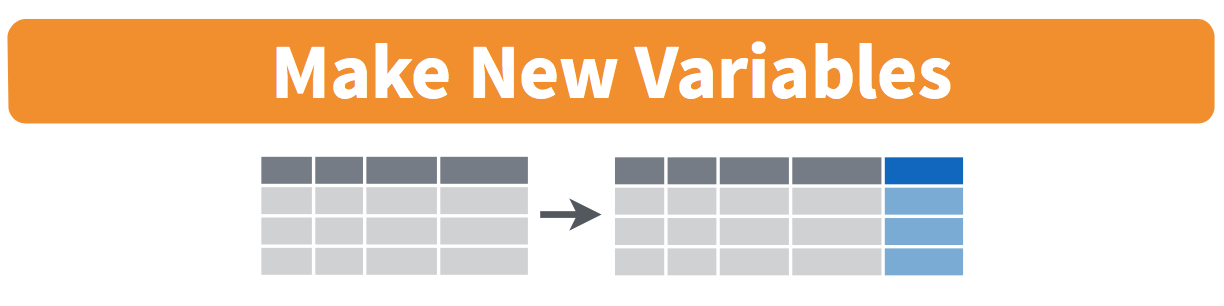
\includegraphics[width=0.8\linewidth,height=0.8\textheight]{images/cheatsheets/mutate} 

}

\caption{Diagram of mutate() columns.}\label{fig:select}
\end{figure}

Another common transformation of data is to create/compute new variables based on existing ones. For example, say you are more comfortable thinking of temperature in degrees Celsius (°C) instead of degrees Fahrenheit (°F). The formula to convert temperatures from °F to °C is

\[
\text{temp in C} = \frac{\text{temp in F} - 32}{1.8}
\]

We can apply this formula to the \texttt{temp} variable using the \texttt{mutate()} \index{R packages!dplyr!mutate()} function from the \texttt{dplyr} package, which takes existing variables and mutates them to create new ones.

\begin{Shaded}
\begin{Highlighting}[]
\NormalTok{weather }\OtherTok{\textless{}{-}}\NormalTok{ weather }\SpecialCharTok{|\textgreater{}} 
  \FunctionTok{mutate}\NormalTok{(}\AttributeTok{temp\_in\_C =}\NormalTok{ (temp }\SpecialCharTok{{-}} \DecValTok{32}\NormalTok{) }\SpecialCharTok{/} \FloatTok{1.8}\NormalTok{)}
\end{Highlighting}
\end{Shaded}

In this code, we \texttt{mutate()} the \texttt{weather} data frame by creating a new variable

\texttt{temp\_in\_C\ =\ (temp\ -\ 32)\ /\ 1.8},

and then we \emph{overwrite} the original \texttt{weather} data frame. Why did we overwrite the data frame \texttt{weather}, instead of assigning the result to a new data frame like \texttt{weather\_new}?

As a rough rule of thumb, as long as you are not losing original information that you might need later, it's acceptable practice to overwrite existing data frames with updated ones, as we did here. On the other hand, why did we not overwrite the variable \texttt{temp}, but instead created a new variable called \texttt{temp\_in\_C}? Because if we did this, we would have erased the original information contained in \texttt{temp} of temperatures in Fahrenheit that may still be valuable to us.

Let's now compute monthly average temperatures in both °F and °C using the \texttt{group\_by()} and \texttt{summarize()} code we saw in Section \ref{groupby}:

\begin{Shaded}
\begin{Highlighting}[]
\NormalTok{summary\_monthly\_temp }\OtherTok{\textless{}{-}}\NormalTok{ weather }\SpecialCharTok{|\textgreater{}} 
  \FunctionTok{group\_by}\NormalTok{(month) }\SpecialCharTok{|\textgreater{}} 
  \FunctionTok{summarize}\NormalTok{(}\AttributeTok{mean\_temp\_in\_F =} \FunctionTok{mean}\NormalTok{(temp, }\AttributeTok{na.rm =} \ConstantTok{TRUE}\NormalTok{), }
            \AttributeTok{mean\_temp\_in\_C =} \FunctionTok{mean}\NormalTok{(temp\_in\_C, }\AttributeTok{na.rm =} \ConstantTok{TRUE}\NormalTok{))}
\NormalTok{summary\_monthly\_temp}
\end{Highlighting}
\end{Shaded}

\begin{verbatim}
# A tibble: 12 x 3
   month mean_temp_in_F mean_temp_in_C
   <int>          <dbl>          <dbl>
 1     1           35.7           2.04
 2     2           34.5           1.39
 3     3           45.0           7.24
 4     4           54.6          12.6 
 5     5           53.6          12.0 
 6     6           69.2          20.6 
 7     7           78.4          25.8 
 8     8           72.8          22.7 
 9     9           64.7          18.1 
10    10           64.2          17.9 
11    11           47.5           8.64
12    12           45.9           7.72
\end{verbatim}

Let's consider another example. Passengers are often frustrated when their flight departs late, but aren't as annoyed if, in the end, pilots can make up some time during the flight. This is known in the airline industry as \emph{gain}, and we will create this variable using the \texttt{mutate()} function:

\begin{Shaded}
\begin{Highlighting}[]
\NormalTok{flights }\OtherTok{\textless{}{-}}\NormalTok{ flights }\SpecialCharTok{|\textgreater{}} 
  \FunctionTok{mutate}\NormalTok{(}\AttributeTok{gain =}\NormalTok{ dep\_delay }\SpecialCharTok{{-}}\NormalTok{ arr\_delay)}
\end{Highlighting}
\end{Shaded}

Let's take a look at only the \texttt{dep\_delay}, \texttt{arr\_delay}, and the resulting \texttt{gain} variables for the first 5 rows in our updated \texttt{flights} data frame in Table \ref{tab:first-five-flights}.

\begin{table}[H]
\centering
\caption{\label{tab:first-five-flights}First five rows of departure/arrival delay and gain variables}
\centering
\begin{tabular}[t]{r|r|r}
\hline
dep\_delay & arr\_delay & gain\\
\hline
203 & 205 & -2\\
\hline
78 & 53 & 25\\
\hline
47 & 34 & 13\\
\hline
173 & 166 & 7\\
\hline
228 & 211 & 17\\
\hline
\end{tabular}
\end{table}

The flight in the first row departed 203 minutes late but arrived 205 minutes late, so its ``gained time in the air'' is a gain of -2 minutes, hence its \texttt{gain} is \(203 - 205 = -2\), which is a \texttt{loss} of 2 minutes. On the other hand, the flight in the third row departed late (\texttt{dep\_delay} of 47) but arrived 34 minutes late (\texttt{arr\_delay} of 34), so its ``gained time in the air'' is \(47 - 34 = 13\) minutes, hence its \texttt{gain} is 13.

Let's look at some summary statistics of the \texttt{gain} variable by considering multiple summary functions at once in the same \texttt{summarize()} code:

\begin{Shaded}
\begin{Highlighting}[]
\NormalTok{gain\_summary }\OtherTok{\textless{}{-}}\NormalTok{ flights }\SpecialCharTok{|\textgreater{}} 
  \FunctionTok{summarize}\NormalTok{(}
    \AttributeTok{min =} \FunctionTok{min}\NormalTok{(gain, }\AttributeTok{na.rm =} \ConstantTok{TRUE}\NormalTok{),}
    \AttributeTok{q1 =} \FunctionTok{quantile}\NormalTok{(gain, }\FloatTok{0.25}\NormalTok{, }\AttributeTok{na.rm =} \ConstantTok{TRUE}\NormalTok{),}
    \AttributeTok{median =} \FunctionTok{quantile}\NormalTok{(gain, }\FloatTok{0.5}\NormalTok{, }\AttributeTok{na.rm =} \ConstantTok{TRUE}\NormalTok{),}
    \AttributeTok{q3 =} \FunctionTok{quantile}\NormalTok{(gain, }\FloatTok{0.75}\NormalTok{, }\AttributeTok{na.rm =} \ConstantTok{TRUE}\NormalTok{),}
    \AttributeTok{max =} \FunctionTok{max}\NormalTok{(gain, }\AttributeTok{na.rm =} \ConstantTok{TRUE}\NormalTok{),}
    \AttributeTok{mean =} \FunctionTok{mean}\NormalTok{(gain, }\AttributeTok{na.rm =} \ConstantTok{TRUE}\NormalTok{),}
    \AttributeTok{sd =} \FunctionTok{sd}\NormalTok{(gain, }\AttributeTok{na.rm =} \ConstantTok{TRUE}\NormalTok{),}
    \AttributeTok{missing =} \FunctionTok{sum}\NormalTok{(}\FunctionTok{is.na}\NormalTok{(gain))}
\NormalTok{  )}
\NormalTok{gain\_summary}
\end{Highlighting}
\end{Shaded}

\begin{verbatim}
# A tibble: 1 x 8
    min    q1 median    q3   max  mean    sd missing
  <dbl> <dbl>  <dbl> <dbl> <dbl> <dbl> <dbl>   <int>
1  -321     1     11    20   101  9.35  18.4   12534
\end{verbatim}

We see for example that the median gain is 11 minutes, while the largest is +101 minutes and the largest negative gain (or loss) at -321 minutes! However, this code would take some time to type out in practice. We'll see later on in Subsection \ref{model1EDA} that there is a much more succinct way to compute a variety of common summary statistics: using the \texttt{tidy\_summary()} function from the \texttt{moderndive} package.

Recall from Section \ref{histograms} that since \texttt{gain} is a numerical variable, we can visualize its distribution using a histogram.

\begin{Shaded}
\begin{Highlighting}[]
\FunctionTok{ggplot}\NormalTok{(}\AttributeTok{data =}\NormalTok{ flights, }\AttributeTok{mapping =} \FunctionTok{aes}\NormalTok{(}\AttributeTok{x =}\NormalTok{ gain)) }\SpecialCharTok{+}
  \FunctionTok{geom\_histogram}\NormalTok{(}\AttributeTok{color =} \StringTok{"white"}\NormalTok{, }\AttributeTok{bins =} \DecValTok{20}\NormalTok{)}
\end{Highlighting}
\end{Shaded}

\begin{figure}[H]

{\centering 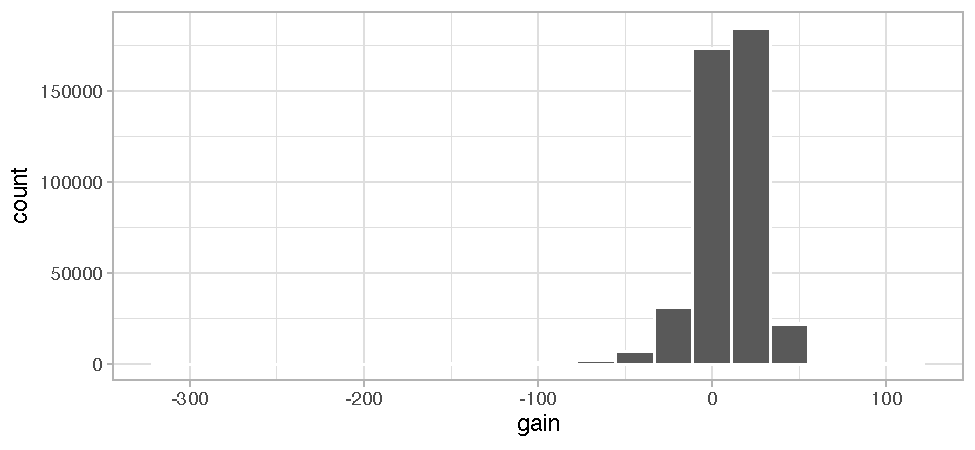
\includegraphics[width=\textwidth]{ModernDive_files/figure-latex/gain-hist-1} 

}

\caption{Histogram of gain variable.}\label{fig:gain-hist}
\end{figure}

The resulting histogram in Figure \ref{fig:gain-hist} provides additional perspective on the \texttt{gain} variable than the summary statistics we computed earlier. For example, note that most values of \texttt{gain} are right around 0.

To close out our discussion on the \texttt{mutate()} function to create new variables, note that we can create multiple new variables at once in the same \texttt{mutate()} code. Furthermore, within the same \texttt{mutate()} code we can refer to new variables we just created. As an example, consider the \texttt{mutate()} code Hadley Wickham \index{Wickham, Hadley} and Garrett Grolemund \index{Grolemund, Garrett} show in Chapter 5 of \emph{R for Data Science} \citep{rds2016}:

\begin{Shaded}
\begin{Highlighting}[]
\NormalTok{flights }\OtherTok{\textless{}{-}}\NormalTok{ flights }\SpecialCharTok{|\textgreater{}} 
  \FunctionTok{mutate}\NormalTok{(}
    \AttributeTok{gain =}\NormalTok{ dep\_delay }\SpecialCharTok{{-}}\NormalTok{ arr\_delay,}
    \AttributeTok{hours =}\NormalTok{ air\_time }\SpecialCharTok{/} \DecValTok{60}\NormalTok{,}
    \AttributeTok{gain\_per\_hour =}\NormalTok{ gain }\SpecialCharTok{/}\NormalTok{ hours}
\NormalTok{  )}
\end{Highlighting}
\end{Shaded}

\begin{learncheck}
\vspace{-0.15in}

\textbf{\emph{Learning check}} \vspace{-0.1in}
\end{learncheck}

\textbf{(LC3.10)} What do positive values of the \texttt{gain} variable in \texttt{flights} correspond to? What about negative values? And what about a zero value?

\textbf{(LC3.11)} Could we create the \texttt{dep\_delay} and \texttt{arr\_delay} columns by simply subtracting \texttt{dep\_time} from \texttt{sched\_dep\_time} and similarly for arrivals? Try the code out and explain any differences between the result and what actually appears in \texttt{flights}.

\textbf{(LC3.12)} What can we say about the distribution of \texttt{gain}? Describe it in a few sentences using the plot and the \texttt{gain\_summary} data frame values.

\begin{learncheck}
\vspace{-0.25in}
\vspace{-0.25in}
\end{learncheck}

\section{\texorpdfstring{\texttt{arrange} and sort rows}{arrange and sort rows}}\label{arrange}

One of the most commonly performed data wrangling tasks is to sort a data frame's rows in the alphanumeric order of one of the variables. The \texttt{dplyr} package's \texttt{arrange()} function \index{R packages!dplyr!arrange()} allows us to sort/reorder a data frame's rows according to the values of the specified variable.

Suppose we are interested in determining the most frequent destination airports for all domestic flights departing from New York City in 2023:

\begin{Shaded}
\begin{Highlighting}[]
\NormalTok{freq\_dest }\OtherTok{\textless{}{-}}\NormalTok{ flights }\SpecialCharTok{|\textgreater{}} 
  \FunctionTok{group\_by}\NormalTok{(dest) }\SpecialCharTok{|\textgreater{}} 
  \FunctionTok{summarize}\NormalTok{(}\AttributeTok{num\_flights =} \FunctionTok{n}\NormalTok{())}
\NormalTok{freq\_dest}
\end{Highlighting}
\end{Shaded}

\begin{verbatim}
# A tibble: 118 x 2
   dest  num_flights
   <chr>       <int>
 1 ABQ           228
 2 ACK           916
 3 AGS            20
 4 ALB          1581
 5 ANC            95
 6 ATL         17570
 7 AUS          4848
 8 AVL          1617
 9 AVP           145
10 BDL           701
# i 108 more rows
\end{verbatim}

Observe that by default the rows of the resulting \texttt{freq\_dest} data frame are sorted in alphabetical order of \texttt{dest}ination. Say instead we would like to see the same data, but sorted from the most to the least number of flights (\texttt{num\_flights}) instead:

\begin{Shaded}
\begin{Highlighting}[]
\NormalTok{freq\_dest }\SpecialCharTok{|\textgreater{}} 
  \FunctionTok{arrange}\NormalTok{(num\_flights)}
\end{Highlighting}
\end{Shaded}

\begin{verbatim}
# A tibble: 118 x 2
   dest  num_flights
   <chr>       <int>
 1 LEX             1
 2 AGS            20
 3 OGG            20
 4 SBN            24
 5 HDN            28
 6 PNS            71
 7 MTJ            77
 8 ANC            95
 9 VPS           109
10 AVP           145
# i 108 more rows
\end{verbatim}

This is, however, the opposite of what we want. The rows are sorted with the least frequent destination airports displayed first. This is because \texttt{arrange()} always returns rows sorted in ascending order by default. To switch the ordering to be in ``descending'' order instead, we use the \texttt{desc()} \index{R packages!dplyr!desc()} function as so:

\begin{Shaded}
\begin{Highlighting}[]
\NormalTok{freq\_dest }\SpecialCharTok{|\textgreater{}} 
  \FunctionTok{arrange}\NormalTok{(}\FunctionTok{desc}\NormalTok{(num\_flights))}
\end{Highlighting}
\end{Shaded}

\begin{verbatim}
# A tibble: 118 x 2
   dest  num_flights
   <chr>       <int>
 1 BOS         19036
 2 ORD         18200
 3 MCO         17756
 4 ATL         17570
 5 MIA         16076
 6 LAX         15968
 7 FLL         14239
 8 CLT         12866
 9 DFW         11675
10 SFO         11651
# i 108 more rows
\end{verbatim}

\section{\texorpdfstring{\texttt{join} data frames}{join data frames}}\label{joins}

Another common data transformation task is ``joining'' or ``merging'' two different datasets. For example, in the \texttt{flights} data frame, the variable \texttt{carrier} lists the carrier code for the different flights. While the corresponding airline names for \texttt{"UA"} and \texttt{"AA"} might be somewhat easy to guess (United and American Airlines), what airlines have codes \texttt{"VX"}, \texttt{"HA"}, and \texttt{"B6"}? This information is provided in a separate data frame \texttt{airlines}.

\begin{Shaded}
\begin{Highlighting}[]
\FunctionTok{View}\NormalTok{(airlines)}
\end{Highlighting}
\end{Shaded}

We see that in \texttt{airlines}, \texttt{carrier} is the carrier code, while \texttt{name} is the full name of the airline company. Using this table, we can see that \texttt{"G4"}, \texttt{"HA"}, and \texttt{"B6"} correspond to Allegiant Air, Hawaiian Airlines, and JetBlue, respectively. However, wouldn't it be nice to have all this information in a single data frame instead of two separate data frames? We can do this by ``joining'' the \texttt{flights} and \texttt{airlines} data frames.

The values in the variable \texttt{carrier} in the \texttt{flights} data frame match the values in the variable \texttt{carrier} in the \texttt{airlines} data frame. In this case, we can use the variable \texttt{carrier} as a \index{joining data!key variable} \emph{key variable} to match the rows of the two data frames. Key variables are almost always \emph{identification variables} that uniquely identify the observational units as we saw in Subsection \ref{identification-vs-measurement-variables}. This ensures that rows in both data frames are appropriately matched during the join. Hadley and Garrett \citep{rds2016} created the diagram in Figure \ref{fig:reldiagram} to show how the different data frames in the \texttt{nycflights23} package are linked by various key variables:



\begin{figure}[H]

{\centering 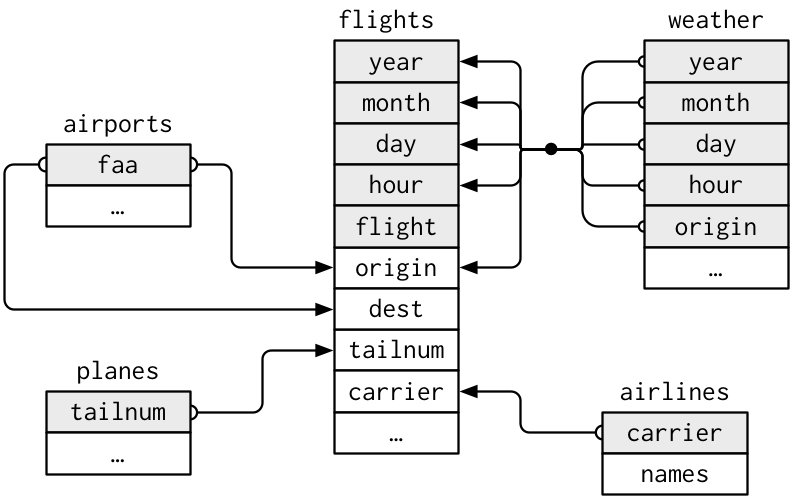
\includegraphics[width=0.65\linewidth,height=0.65\textheight]{images/r4ds/relational-nycflights} 

}

\caption{Data relationships in nycflights from \emph{R for Data Science}.}\label{fig:reldiagram}
\end{figure}

\subsection{Matching key variable names}\label{matching-key-variable-names}

In both the \texttt{flights} and \texttt{airlines} data frames, the key variable we want to join/merge/match the rows by has the same name: \texttt{carrier}. Let's use the \texttt{inner\_join()} \index{R packages!dplyr!inner\_join()} function to join the two data frames, where the rows will be matched by the variable \texttt{carrier}, and then compare the resulting data frames:

\begin{Shaded}
\begin{Highlighting}[]
\NormalTok{flights\_joined }\OtherTok{\textless{}{-}}\NormalTok{ flights }\SpecialCharTok{|\textgreater{}} 
  \FunctionTok{inner\_join}\NormalTok{(airlines, }\AttributeTok{by =} \StringTok{"carrier"}\NormalTok{)}
\FunctionTok{View}\NormalTok{(flights)}
\FunctionTok{View}\NormalTok{(flights\_joined)}
\end{Highlighting}
\end{Shaded}

Observe that the \texttt{flights} and \texttt{flights\_joined} data frames are identical except that \texttt{flights\_joined} has an additional variable \texttt{name}. The values of \texttt{name} correspond to the airline companies' names as indicated in the \texttt{airlines} data frame.

A visual representation of the \texttt{inner\_join()} is shown in Figure \ref{fig:ijdiagram} \citep{rds2016}. There are other types of joins available (such as \texttt{left\_join()}, \texttt{right\_join()}, \texttt{outer\_join()}, and \texttt{anti\_join()}), but the \texttt{inner\_join()} will solve nearly all of the problems you'll encounter in this book.



\begin{figure}[H]

{\centering \includegraphics[width=\textwidth,height=1.2\textheight]{images/r4ds/join-inner} 

}

\caption{Diagram of inner join from \emph{R for Data Science}.}\label{fig:ijdiagram}
\end{figure}

\subsection{Different key variable names}\label{diff-key}

Say instead you are interested in the destinations of all domestic flights departing NYC in 2023, and you ask yourself questions like: ``What cities are these airports in?'', or ``Is \texttt{"ORD"} Orlando?'', or ``Where is \texttt{"FLL"}?''.

The \texttt{airports} data frame contains the airport codes for each airport:

\begin{Shaded}
\begin{Highlighting}[]
\FunctionTok{View}\NormalTok{(airports)}
\end{Highlighting}
\end{Shaded}

However, if you look at both the \texttt{airports} and \texttt{flights} data frames, you'll find that the airport codes are in variables that have different names. In \texttt{airports} the airport code is in \texttt{faa}, whereas in \texttt{flights} the airport codes are in \texttt{origin} and \texttt{dest}. This fact is further highlighted in the visual representation of the relationships between these data frames in Figure \ref{fig:reldiagram}.

In order to join these two data frames by airport code, our \texttt{inner\_join()} operation will use the \texttt{by\ =\ c("dest"\ =\ "faa")} \index{R packages!dplyr!inner\_join()!by} argument with modified code syntax allowing us to join two data frames where the key variable has a different name:

\begin{Shaded}
\begin{Highlighting}[]
\NormalTok{flights\_with\_airport\_names }\OtherTok{\textless{}{-}}\NormalTok{ flights }\SpecialCharTok{|\textgreater{}} 
  \FunctionTok{inner\_join}\NormalTok{(airports, }\AttributeTok{by =} \FunctionTok{c}\NormalTok{(}\StringTok{"dest"} \OtherTok{=} \StringTok{"faa"}\NormalTok{))}
\FunctionTok{View}\NormalTok{(flights\_with\_airport\_names)}
\end{Highlighting}
\end{Shaded}

Let's construct the chain of pipe operators \texttt{\textbar{}\textgreater{}} that computes the number of flights from NYC to each destination, but also includes information about each destination airport:

\begin{Shaded}
\begin{Highlighting}[]
\NormalTok{named\_dests }\OtherTok{\textless{}{-}}\NormalTok{ flights }\SpecialCharTok{|\textgreater{}}
  \FunctionTok{group\_by}\NormalTok{(dest) }\SpecialCharTok{|\textgreater{}}
  \FunctionTok{summarize}\NormalTok{(}\AttributeTok{num\_flights =} \FunctionTok{n}\NormalTok{()) }\SpecialCharTok{|\textgreater{}}
  \FunctionTok{arrange}\NormalTok{(}\FunctionTok{desc}\NormalTok{(num\_flights)) }\SpecialCharTok{|\textgreater{}}
  \FunctionTok{inner\_join}\NormalTok{(airports, }\AttributeTok{by =} \FunctionTok{c}\NormalTok{(}\StringTok{"dest"} \OtherTok{=} \StringTok{"faa"}\NormalTok{)) }\SpecialCharTok{|\textgreater{}}
  \FunctionTok{rename}\NormalTok{(}\AttributeTok{airport\_name =}\NormalTok{ name)}
\NormalTok{named\_dests}
\end{Highlighting}
\end{Shaded}

\begin{verbatim}
# A tibble: 114 x 9
   dest  num_flights airport_name        lat    lon   alt    tz dst   tzone
   <chr>       <int> <chr>             <dbl>  <dbl> <dbl> <dbl> <chr> <chr>
 1 BOS         19036 General Edward L~  42.4  -71.0    20    -5 A     Amer~
 2 ORD         18200 Chicago O'Hare I~  42.0  -87.9   672    -6 A     Amer~
 3 MCO         17756 Orlando Internat~  28.4  -81.3    96    -5 A     Amer~
 4 ATL         17570 Hartsfield Jacks~  33.6  -84.4  1026    -5 A     Amer~
 5 MIA         16076 Miami Internatio~  25.8  -80.3     8    -5 A     Amer~
 6 LAX         15968 Los Angeles Inte~  33.9 -118.    125    -8 A     Amer~
 7 FLL         14239 Fort Lauderdale ~  26.1  -80.2     9    -5 A     Amer~
 8 CLT         12866 Charlotte Dougla~  35.2  -80.9   748    -5 A     Amer~
 9 DFW         11675 Dallas Fort Wort~  32.9  -97.0   607    -6 A     Amer~
10 SFO         11651 San Francisco In~  37.6 -122.     13    -8 A     Amer~
# i 104 more rows
\end{verbatim}

In case you didn't know, \texttt{"ORD"} is the airport code of Chicago O'Hare airport and \texttt{"FLL"} is the main airport in Fort Lauderdale, Florida, which can be seen in the \texttt{airport\_name} variable.

\subsection{Multiple key variables}\label{multiple-key-variables}

Say instead we want to join two data frames by \emph{multiple key variables}. For example, in Figure \ref{fig:reldiagram}, we see that in order to join the \texttt{flights} and \texttt{weather} data frames, we need more than one key variable: \texttt{year}, \texttt{month}, \texttt{day}, \texttt{hour}, and \texttt{origin}. This is because the combination of these 5 variables act to uniquely identify each observational unit in the \texttt{weather} data frame: hourly weather recordings at each of the 3 NYC airports.

We achieve this by specifying a \emph{vector} of key variables to join by using the \texttt{c()} function. Recall from Subsection \ref{programming-concepts} that \texttt{c()} is short for ``combine'' or ``concatenate.'' \index{vectors}

\begin{Shaded}
\begin{Highlighting}[]
\NormalTok{flights\_weather\_joined }\OtherTok{\textless{}{-}}\NormalTok{ flights }\SpecialCharTok{|\textgreater{}}
  \FunctionTok{inner\_join}\NormalTok{(weather, }\AttributeTok{by =} \FunctionTok{c}\NormalTok{(}\StringTok{"year"}\NormalTok{, }\StringTok{"month"}\NormalTok{, }\StringTok{"day"}\NormalTok{, }\StringTok{"hour"}\NormalTok{, }\StringTok{"origin"}\NormalTok{))}
\FunctionTok{View}\NormalTok{(flights\_weather\_joined)}
\end{Highlighting}
\end{Shaded}

\begin{learncheck}
\vspace{-0.15in}

\textbf{\emph{Learning check}} \vspace{-0.1in}
\end{learncheck}

\textbf{(LC3.13)} Looking at Figure \ref{fig:reldiagram}, when joining \texttt{flights} and \texttt{weather} (or, in other words, matching the hourly weather values with each flight), why do we need to join by all of \texttt{year}, \texttt{month}, \texttt{day}, \texttt{hour}, and \texttt{origin}, and not just \texttt{hour}?

\textbf{(LC3.14)} What surprises you about the top 10 destinations from NYC in 2023?

\begin{learncheck}
\vspace{-0.25in}
\vspace{-0.25in}
\end{learncheck}

\subsection{Normal forms}\label{normal-forms}

The data frames included in the \texttt{nycflights23} package are in a form that minimizes redundancy of data. For example, the \texttt{flights} data frame only saves the \texttt{carrier} code of the airline company; it does not include the actual name of the airline. For example, you'll see that the first row of \texttt{flights} has \texttt{carrier} equal to \texttt{UA}, but it does not include the airline name of ``United Air Lines Inc.''

The names of the airline companies are included in the \texttt{name} variable of the \texttt{airlines} data frame. In order to have the airline company name included in \texttt{flights}, we could join these two data frames as follows:

\begin{Shaded}
\begin{Highlighting}[]
\NormalTok{joined\_flights }\OtherTok{\textless{}{-}}\NormalTok{ flights }\SpecialCharTok{|\textgreater{}} 
  \FunctionTok{inner\_join}\NormalTok{(airlines, }\AttributeTok{by =} \StringTok{"carrier"}\NormalTok{)}
\FunctionTok{View}\NormalTok{(joined\_flights)}
\end{Highlighting}
\end{Shaded}

We are capable of performing this join because each of the data frames have \emph{keys} in common to relate one to another: the \texttt{carrier} variable in both the \texttt{flights} and \texttt{airlines} data frames. The \emph{key} variable(s) that we base our joins on are often \emph{identification variables} as we mentioned previously.

This is an important property of what's known as \emph{normal forms} of data. The process of decomposing data frames into less redundant tables without losing information is called \emph{normalization}. More information is available on \href{https://en.wikipedia.org/wiki/Database_normalization}{Wikipedia}.

Both \texttt{dplyr} and \href{https://en.wikipedia.org/wiki/SQL}{SQL} we mentioned in the introduction of this chapter use such \emph{normal forms}. Given that they share such commonalities, once you learn either of these two tools, you can learn the other very easily.

\begin{learncheck}
\vspace{-0.15in}

\textbf{\emph{Learning check}} \vspace{-0.1in}
\end{learncheck}

\textbf{(LC3.15)} What are some advantages of data in normal forms? What are some disadvantages?

\begin{learncheck}
\vspace{-0.25in}
\vspace{-0.25in}
\end{learncheck}

\section{Other verbs}\label{other-verbs}

Here are some other useful data wrangling verbs:

\begin{itemize}
\tightlist
\item
  \texttt{select()} only a subset of variables/columns.
\item
  \texttt{relocate()} variables/columns to a new position.
\item
  \texttt{rename()} variables/columns to have new names.
\item
  Return only the \texttt{top\_n()} values of a variable.
\end{itemize}

\subsection{\texorpdfstring{\texttt{select} variables}{select variables}}\label{select}

\begin{figure}[H]

{\centering \includegraphics[width=\textwidth]{images/cheatsheets/select} 

}

\caption{Diagram of select() columns.}\label{fig:selectfig}
\end{figure}

We've seen that the \texttt{flights} data frame in the \texttt{nycflights23} package contains 19 different variables. You can identify the names of these 19 variables by running the \texttt{glimpse()} function from the \texttt{dplyr} package:

\begin{Shaded}
\begin{Highlighting}[]
\FunctionTok{glimpse}\NormalTok{(flights)}
\end{Highlighting}
\end{Shaded}

However, say you only need two of these 19 variables, say \texttt{carrier} and \texttt{flight}. You can \texttt{select()} \index{R packages!dplyr!select()} these two variables:

\begin{Shaded}
\begin{Highlighting}[]
\NormalTok{flights }\SpecialCharTok{|\textgreater{}} 
  \FunctionTok{select}\NormalTok{(carrier, flight)}
\end{Highlighting}
\end{Shaded}

This function makes it easier to explore large datasets since it allows us to limit the scope to only those variables we care most about. For example, if we \texttt{select()} only a smaller number of variables as is shown in Figure \ref{fig:selectfig}, it will make viewing the dataset in RStudio's spreadsheet viewer more digestible.

Let's say instead you want to drop, or de-select, certain variables. For example, consider the variable \texttt{year} in the \texttt{flights} data frame. This variable isn't quite a ``variable'' because it is always \texttt{2023} and hence doesn't change. Say you want to remove this variable from the data frame. We can deselect \texttt{year} by using the \texttt{-} sign:

\begin{Shaded}
\begin{Highlighting}[]
\NormalTok{flights\_no\_year }\OtherTok{\textless{}{-}}\NormalTok{ flights }\SpecialCharTok{|\textgreater{}} \FunctionTok{select}\NormalTok{(}\SpecialCharTok{{-}}\NormalTok{year)}
\end{Highlighting}
\end{Shaded}

Another way of selecting columns/variables is by specifying a range of columns:

\begin{Shaded}
\begin{Highlighting}[]
\NormalTok{flight\_arr\_times }\OtherTok{\textless{}{-}}\NormalTok{ flights }\SpecialCharTok{|\textgreater{}} \FunctionTok{select}\NormalTok{(month}\SpecialCharTok{:}\NormalTok{day, arr\_time}\SpecialCharTok{:}\NormalTok{sched\_arr\_time)}
\NormalTok{flight\_arr\_times}
\end{Highlighting}
\end{Shaded}

This will \texttt{select()} all columns between \texttt{month} and \texttt{day}, as well as between \texttt{arr\_time} and \texttt{sched\_arr\_time}, and drop the rest.

The helper functions \texttt{starts\_with()}, \texttt{ends\_with()}, and \texttt{contains()} can be used to select variables/columns that match those conditions. As examples,

\begin{Shaded}
\begin{Highlighting}[]
\NormalTok{flights }\SpecialCharTok{|\textgreater{}} \FunctionTok{select}\NormalTok{(}\FunctionTok{starts\_with}\NormalTok{(}\StringTok{"a"}\NormalTok{))}
\NormalTok{flights }\SpecialCharTok{|\textgreater{}} \FunctionTok{select}\NormalTok{(}\FunctionTok{ends\_with}\NormalTok{(}\StringTok{"delay"}\NormalTok{))}
\NormalTok{flights }\SpecialCharTok{|\textgreater{}} \FunctionTok{select}\NormalTok{(}\FunctionTok{contains}\NormalTok{(}\StringTok{"time"}\NormalTok{))}
\end{Highlighting}
\end{Shaded}

Lastly, the \texttt{select()} function can also be used to reorder columns when used with the \texttt{everything()} helper function. For example, suppose we want the \texttt{hour}, \texttt{minute}, and \texttt{time\_hour} variables to appear immediately after the \texttt{year}, \texttt{month}, and \texttt{day} variables, while not discarding the rest of the variables. In the following code, \texttt{everything()} will pick up all remaining variables:

\begin{Shaded}
\begin{Highlighting}[]
\NormalTok{flights\_reorder }\OtherTok{\textless{}{-}}\NormalTok{ flights }\SpecialCharTok{|\textgreater{}} 
  \FunctionTok{select}\NormalTok{(year, month, day, hour, minute, time\_hour, }\FunctionTok{everything}\NormalTok{())}
\FunctionTok{glimpse}\NormalTok{(flights\_reorder)}
\end{Highlighting}
\end{Shaded}

\subsection{\texorpdfstring{\texttt{relocate} variables}{relocate variables}}\label{relocate}

Another (usually shorter) way to reorder variables is by using the \index{R packages!dplyr!relocate()} \texttt{relocate()} function. This function allows you to move variables to a new position in the data frame. For example, if we want to move the \texttt{hour}, \texttt{minute}, and \texttt{time\_hour} variables to appear immediately after the \texttt{year}, \texttt{month}, and \texttt{day} variables, we can use the following code:

\begin{Shaded}
\begin{Highlighting}[]
\NormalTok{flights\_relocate }\OtherTok{\textless{}{-}}\NormalTok{ flights }\SpecialCharTok{|\textgreater{}} 
  \FunctionTok{relocate}\NormalTok{(hour, minute, time\_hour, }\AttributeTok{.after =}\NormalTok{ day)}
\FunctionTok{glimpse}\NormalTok{(flights\_relocate)}
\end{Highlighting}
\end{Shaded}

\subsection{\texorpdfstring{\texttt{rename} variables}{rename variables}}\label{rename}

One more useful function is \index{R packages!dplyr!rename()} \texttt{rename()}, which as you may have guessed changes the name of variables. Suppose we want to only focus on \texttt{dep\_time} and \texttt{arr\_time} and change \texttt{dep\_time} and \texttt{arr\_time} to be \texttt{departure\_time} and \texttt{arrival\_time} instead in the \texttt{flights\_time\_new} data frame:

\begin{Shaded}
\begin{Highlighting}[]
\NormalTok{flights\_time\_new }\OtherTok{\textless{}{-}}\NormalTok{ flights }\SpecialCharTok{|\textgreater{}} 
  \FunctionTok{select}\NormalTok{(dep\_time, arr\_time) }\SpecialCharTok{|\textgreater{}} 
  \FunctionTok{rename}\NormalTok{(}\AttributeTok{departure\_time =}\NormalTok{ dep\_time, }\AttributeTok{arrival\_time =}\NormalTok{ arr\_time)}
\FunctionTok{glimpse}\NormalTok{(flights\_time\_new)}
\end{Highlighting}
\end{Shaded}

Note that in this case we used a single \texttt{=} sign within the \texttt{rename()}. For example, \texttt{departure\_time\ =\ dep\_time} renames the \texttt{dep\_time} variable to have the new name \texttt{departure\_time}. This is because we are not testing for equality like we would using \texttt{==}. Instead we want to assign a new variable \texttt{departure\_time} to have the same values as \texttt{dep\_time} and then delete the variable \texttt{dep\_time}. Note that new \texttt{dplyr} users often forget that the new variable name comes before the equal sign.

\subsection{\texorpdfstring{\texttt{top\_n} values of a variable}{top\_n values of a variable}}\label{top_n-values-of-a-variable}

We can also return the top \texttt{n} values of a variable using the \texttt{top\_n()} \index{R packages!dplyr!top\_n()} function. For example, we can return a data frame of the top 10 destination airports using the example from Subsection \ref{diff-key}. Observe that we set the number of values to return to \texttt{n\ =\ 10} and \texttt{wt\ =\ num\_flights} to indicate that we want the rows corresponding to the top 10 values of \texttt{num\_flights}. See the help file for \texttt{top\_n()} by running \texttt{?top\_n} for more information.

\begin{Shaded}
\begin{Highlighting}[]
\NormalTok{named\_dests }\SpecialCharTok{|\textgreater{}} \FunctionTok{top\_n}\NormalTok{(}\AttributeTok{n =} \DecValTok{10}\NormalTok{, }\AttributeTok{wt =}\NormalTok{ num\_flights)}
\end{Highlighting}
\end{Shaded}

Let's further \texttt{arrange()} these results in descending order of \texttt{num\_flights}:

\begin{Shaded}
\begin{Highlighting}[]
\NormalTok{named\_dests }\SpecialCharTok{|\textgreater{}} 
  \FunctionTok{top\_n}\NormalTok{(}\AttributeTok{n =} \DecValTok{10}\NormalTok{, }\AttributeTok{wt =}\NormalTok{ num\_flights) }\SpecialCharTok{|\textgreater{}} 
  \FunctionTok{arrange}\NormalTok{(}\FunctionTok{desc}\NormalTok{(num\_flights))}
\end{Highlighting}
\end{Shaded}

\begin{learncheck}
\vspace{-0.15in}

\textbf{\emph{Learning check}} \vspace{-0.1in}
\end{learncheck}

\textbf{(LC3.16)} What are some ways to select all three of the \texttt{dest}, \texttt{air\_time}, and \texttt{distance} variables from \texttt{flights}? Give the code showing how to do this in at least three different ways.

\textbf{(LC3.17)} How could one use \texttt{starts\_with()}, \texttt{ends\_with()}, and \texttt{contains()} to select columns from the \texttt{flights} data frame? Provide three different examples in total: one for \texttt{starts\_with()}, one for \texttt{ends\_with()}, and one for \texttt{contains()}.

\textbf{(LC3.18)} Why might we want to use the \texttt{select()} function on a data frame?

\textbf{(LC3.19)} Create a new data frame that shows the top 5 airports with the largest arrival delays from NYC in 2023.

\begin{learncheck}
\vspace{-0.25in}
\vspace{-0.25in}
\end{learncheck}

\section{Conclusion}\label{wrangling-conclusion}

\subsection{Summary table}\label{summary-table-1}

Let's recap our data wrangling verbs in Table \ref{tab:wrangle-summary-table}. Using these verbs and the pipe \texttt{\textbar{}\textgreater{}} operator from Section \ref{piping}, you'll be able to write easily legible code to perform almost all the data wrangling and data transformation necessary for the rest of this book.

\begin{table}[H]
\centering
\caption{\label{tab:wrangle-summary-table}Summary of data wrangling verbs}
\centering
\fontsize{10}{12}\selectfont
\begin{tabular}[t]{>{\raggedright\arraybackslash}p{0.9in}>{\raggedright\arraybackslash}p{4in}}
\toprule
Verb & Data wrangling operation\\
\midrule
filter() & Pick out a subset of rows\\
summarize() & Summarize many values to one using a summary statistic function like mean(), median(), etc.\\
group\_by() & Add grouping structure to rows in data frame. Note this does not change values in data frame, rather only the meta-data\\
mutate() & Create new variables by mutating existing ones\\
arrange() & Arrange rows of a data variable in ascending (default) or descending order\\
inner\_join() & Join/merge two data frames, matching rows by a key variable\\
\bottomrule
\end{tabular}
\end{table}

\begin{learncheck}
\vspace{-0.15in}

\textbf{\emph{Learning check}} \vspace{-0.1in}
\end{learncheck}

\textbf{(LC3.20)} Let's now put your newly acquired data wrangling skills to the test!

An airline industry measure of a passenger airline's capacity is the \href{https://en.wikipedia.org/wiki/Available_seat_miles}{available seat miles}, which is equal to the number of seats available multiplied by the number of miles or kilometers flown summed over all flights.

For example, let's consider the scenario in Figure \ref{fig:available-seat-miles}. Since the airplane has 4 seats and it travels 200 miles, the available seat miles are \(4 \times 200 = 800\).

\begin{figure}[H]

{\centering \includegraphics[width=\textwidth,height=0.35\textheight]{images/flowcharts/flowchart/flowchart.012} 

}

\caption{Example of available seat miles for one flight.}\label{fig:available-seat-miles}
\end{figure}

Extending this idea, let's say an airline had 2 flights using a plane with 10 seats that flew 500 miles and 3 flights using a plane with 20 seats that flew 1000 miles, the available seat miles would be \(2 \times 10 \times 500 + 3 \times 20 \times 1000 = 70,000\) seat miles.

Using the datasets included in the \texttt{nycflights23} package, compute the available seat miles for each airline sorted in descending order. After completing all the necessary data wrangling steps, the resulting data frame should have 16 rows (one for each airline) and 2 columns (airline name and available seat miles). Here are some hints:

\begin{enumerate}
\def\labelenumi{\arabic{enumi}.}
\tightlist
\item
  \textbf{Crucial}: Unless you are very confident in what you are doing, it is worthwhile not starting to code right away. Rather, first sketch out on paper all the necessary data wrangling steps not using exact code, but rather high-level \emph{pseudocode} that is informal yet detailed enough to articulate what you are doing. This way you won't confuse \emph{what} you are trying to do (the algorithm) with \emph{how} you are going to do it (writing \texttt{dplyr} code).
\item
  Take a close look at all the datasets using the \texttt{View()} function: \texttt{flights}, \texttt{weather}, \texttt{planes}, \texttt{airports}, and \texttt{airlines} to identify which variables are necessary to compute available seat miles.
\item
  Figure \ref{fig:reldiagram} showing how the various datasets can be joined will also be useful.
\item
  Consider the data wrangling verbs in Table \ref{tab:wrangle-summary-table} as your toolbox!
\end{enumerate}

\begin{learncheck}
\vspace{-0.25in}
\vspace{-0.25in}
\end{learncheck}

\subsection{Additional resources}\label{additional-resources-2}

Solutions to all \emph{Learning checks} can be found in the Appendices of the online version of the book. The Appendices start at \url{https://moderndive.com/v2/appendixa}.

An R script file of all R code used in this chapter is available at \url{https://www.moderndive.com/v2/scripts/03-wrangling.R}.

If you want to further unlock the power of the \texttt{dplyr} package for data wrangling, we suggest that you check out RStudio's ``Data Transformation with dplyr'' cheatsheet. This cheatsheet summarizes much more than what we've discussed in this chapter, in particular more intermediate level and advanced data wrangling functions, while providing quick and easy-to-read visual descriptions. In fact, many of the diagrams illustrating data wrangling operations in this chapter, such as Figure \ref{fig:filter} on \texttt{filter()}, originate from this cheatsheet.

In the current version of RStudio in 2024, you can access this cheatsheet by going to the RStudio Menu Bar -\textgreater{} Help -\textgreater{} Cheatsheets -\textgreater{} ``Data Transformation with dplyr.''

On top of the data wrangling verbs and examples we presented in this section, if you'd like to see more examples of using the \texttt{dplyr} package for data wrangling, check out \href{http://r4ds.had.co.nz/transform.html}{Chapter 5} of \emph{R for Data Science} \citep{rds2016}.

\subsection{What's to come?}\label{whats-to-come-1}

So far in this book, we've explored, visualized, and wrangled data saved in data frames. These data frames were saved in a spreadsheet-like format: in a rectangular shape with a certain number of rows corresponding to observations and a certain number of columns corresponding to variables describing these observations.

We'll see in the upcoming Chapter \ref{tidy} that there are actually two ways to represent data in spreadsheet-type rectangular format: (1) ``wide'' format and (2) ``tall/narrow'' format. The tall/narrow format is also known as \emph{``tidy''} format in R user circles. While the distinction between ``tidy'' and non-``tidy'' formatted data is subtle, it has immense implications for our data science work. This is because almost all the packages used in this book, including the \texttt{ggplot2} package for data visualization and the \texttt{dplyr} package for data wrangling, all assume that all data frames are in ``tidy'' format.

Furthermore, up until now we've only explored, visualized, and wrangled data saved within R packages. But what if you want to analyze data that you have saved in a Microsoft Excel, a Google Sheets, or a ``Comma-Separated Values'' (CSV) file? In Section \ref{csv}, we'll show you how to import this data into R using the \texttt{readr} package.

\chapter{Data Importing and Tidy Data}\label{tidy}

In Subsection \ref{programming-concepts}, we introduced the concept of a \index{data frame} data frame in R: a rectangular spreadsheet-like representation of data where the rows correspond to observations and the columns correspond to variables describing each observation. In Section \ref{nycflights}, we started exploring our first data frame: the \texttt{flights} data frame included in the \texttt{nycflights23} package. In Chapter \ref{viz}, we created visualizations based on the data included in \texttt{flights} and other data frames such as \texttt{weather}. In Chapter \ref{wrangling}, we learned how to take existing data frames and transform/modify them to suit our ends.

In this final chapter of the ``Data Science with \texttt{tidyverse}'' portion of the book, we extend some of these ideas by discussing a type of data formatting called ``tidy'' data. You will see that having data stored in ``tidy'' format is about more than just what the everyday definition of the term ``tidy'' might suggest: having your data ``neatly organized.'' Instead, we define the term ``tidy'' as it's used by data scientists who use R, outlining a set of rules by which data is saved.

Knowledge of this type of data formatting was not necessary for our treatment of data visualization in Chapter \ref{viz} and data wrangling in Chapter \ref{wrangling}. This is because all the data used were already in ``tidy'' format. In this chapter, we'll now see that this format is essential to using the tools we covered up until now. Furthermore, it will also be useful for all subsequent chapters in this book when we cover regression and statistical inference. First, however, we'll show you how to import spreadsheet data in R.

\subsection*{Needed packages}\label{tidy-packages}


Let's load all the packages needed for this chapter (this assumes you've already installed them). If needed, read Section \ref{packages} for information on how to install and load R packages.

\begin{Shaded}
\begin{Highlighting}[]
\FunctionTok{library}\NormalTok{(dplyr)}
\FunctionTok{library}\NormalTok{(ggplot2)}
\FunctionTok{library}\NormalTok{(readr)}
\FunctionTok{library}\NormalTok{(tidyr)}
\FunctionTok{library}\NormalTok{(nycflights23)}
\FunctionTok{library}\NormalTok{(fivethirtyeight)}
\end{Highlighting}
\end{Shaded}

Note that when you load the \texttt{fivethirtyeight} package, you'll receive the following message:

\begin{quote}
Some larger datasets need to be installed separately, like senators and house\_district\_forecast. To install these, we recommend you
install the fivethirtyeightdata package by running: install.packages(`fivethirtyeightdata', repos =
`\url{https://fivethirtyeightdata.github.io/drat/}', type = `source')
\end{quote}

This message can be ignored for the purposes of this book, but if you'd like to explore these larger datasets, you can install the \texttt{fivethirtyeightdata} package as suggested.

\section{Importing data}\label{csv}

Up to this point, we've almost entirely used data stored inside of an R package. Say instead you have your own data saved on your computer or somewhere online. How can you analyze this data in R? Spreadsheet data is often saved in one of the following three formats:

First, a \emph{Comma Separated Values} \texttt{.csv} \index{CSV file} file. You can think of a \texttt{.csv} file as a bare-bones spreadsheet where:

\begin{itemize}
\tightlist
\item
  Each line in the file corresponds to one row of data/one observation.
\item
  Values for each line are separated with commas. In other words, the values of different variables are separated by commas in each row.
\item
  The first line is often, but not always, a \emph{header} row indicating the names of the columns/variables.
\end{itemize}

Second, an Excel \texttt{.xlsx} spreadsheet file. This format is based on Microsoft's proprietary Excel software. As opposed to bare-bones \texttt{.csv} files, \texttt{.xlsx} Excel files contain a lot of meta-data\index{meta-data} (data about data). Recall we saw a previous example of meta-data in Section \ref{groupby} when adding ``group structure'' meta-data to a data frame by using the \texttt{group\_by()} verb. Some examples of Excel spreadsheet meta-data include the use of bold and italic fonts, colored cells, different column widths, and formula macros.

Third, a \href{https://www.google.com/sheets/about/}{Google Sheets} file, which is a ``cloud'' or online-based way to work with a spreadsheet. Google Sheets allows you to download your data in both comma separated values \texttt{.csv} and Excel \texttt{.xlsx} formats. One way to import Google Sheets data in R is to go to the Google Sheets menu bar -\textgreater{} File -\textgreater{} Download as -\textgreater{} Select ``Microsoft Excel'' or ``Comma-separated values'' and then load that data into R. A more advanced way to import Google Sheets data in R is by using the \href{https://googlesheets4.tidyverse.org/}{\texttt{googlesheets4}} package, a method we leave to a more advanced data science book.

We'll cover two methods for importing \texttt{.csv} and \texttt{.xlsx} spreadsheet data in R: one using the console and the other using RStudio's graphical user interface, abbreviated as ``GUI.''

\subsection{Using the console}\label{using-the-console}

First, let's import a Comma Separated Values \texttt{.csv} file that exists on the internet. The \texttt{.csv} file \texttt{dem\_score.csv} contains ratings of the level of democracy in different countries spanning 1952 to 1992 and is accessible at \url{https://moderndive.com/data/dem_score.csv}. Let's use the \texttt{read\_csv()} function from the \texttt{readr} \index{R packages!readr!read\_csv()} \citep{R-readr} package to read it off the web, import it into R, and save it in a data frame called \texttt{dem\_score}.

\begin{Shaded}
\begin{Highlighting}[]
\FunctionTok{library}\NormalTok{(readr)}
\NormalTok{dem\_score }\OtherTok{\textless{}{-}} \FunctionTok{read\_csv}\NormalTok{(}\StringTok{"https://moderndive.com/data/dem\_score.csv"}\NormalTok{)}
\NormalTok{dem\_score}
\end{Highlighting}
\end{Shaded}

\begin{verbatim}
# A tibble: 96 x 10
   country   `1952` `1957` `1962` `1967` `1972` `1977` `1982` `1987` `1992`
   <chr>      <dbl>  <dbl>  <dbl>  <dbl>  <dbl>  <dbl>  <dbl>  <dbl>  <dbl>
 1 Albania       -9     -9     -9     -9     -9     -9     -9     -9      5
 2 Argentina     -9     -1     -1     -9     -9     -9     -8      8      7
 3 Armenia       -9     -7     -7     -7     -7     -7     -7     -7      7
 4 Australia     10     10     10     10     10     10     10     10     10
 5 Austria       10     10     10     10     10     10     10     10     10
 6 Azerbaij~     -9     -7     -7     -7     -7     -7     -7     -7      1
 7 Belarus       -9     -7     -7     -7     -7     -7     -7     -7      7
 8 Belgium       10     10     10     10     10     10     10     10     10
 9 Bhutan       -10    -10    -10    -10    -10    -10    -10    -10    -10
10 Bolivia       -4     -3     -3     -4     -7     -7      8      9      9
# i 86 more rows
\end{verbatim}

In this \texttt{dem\_score} data frame, the minimum value of \texttt{-10} corresponds to a highly autocratic nation, whereas a value of \texttt{10} corresponds to a highly democratic nation. Note also that backticks surround the different variable names. Variable names in R by default are not allowed to start with a number nor include spaces, but we can get around this fact by surrounding the column name with backticks. We'll revisit the \texttt{dem\_score} data frame in a case study in the upcoming Section \ref{case-study-tidy}.

Note that the \texttt{read\_csv()} function included in the \texttt{readr} package is different than the \texttt{read.csv()} function that comes installed with R. While the difference in the names might seem trivial (an \texttt{\_} instead of a \texttt{.}), the \texttt{read\_csv()} function is, in our opinion, easier to use since it can more easily read data off the web and generally imports data at a much faster speed. Furthermore, the \texttt{read\_csv()} function included in the \texttt{readr} saves data frames as \texttt{tibbles} by default.

\subsection{Using RStudio's interface}\label{using-rstudios-interface}

Let's read in the exact same data, but this time from an Excel file saved on your computer. Furthermore, we'll do this using RStudio's graphical interface instead of running \texttt{read\_csv()} in the console. First, download the Excel file \texttt{dem\_score.xlsx} by going to https://moderndive.com/data/dem\_score.xlsx, then

\begin{enumerate}
\def\labelenumi{\arabic{enumi}.}
\tightlist
\item
  Go to the Files pane of RStudio.
\item
  Navigate to the directory (i.e., folder on your computer) where the downloaded \texttt{dem\_score.xlsx} Excel file is saved. For example, this might be in your Downloads folder.
\item
  Click on \texttt{dem\_score.xlsx}.
\item
  Click ``Import Dataset\ldots{}''
\end{enumerate}

At this point, you should see a screen pop-up like in Figure \ref{fig:read-excel}. After clicking on the ``Import'' \index{RStudio!import data} button on the bottom right of Figure \ref{fig:read-excel}, RStudio will save this spreadsheet's data in a data frame called \texttt{dem\_score} and display its contents in the spreadsheet viewer.

\begin{figure}[H]

{\centering \includegraphics[width=\textwidth]{images/rstudio_screenshots/read_excel} 

}

\caption{Importing an Excel file to R.}\label{fig:read-excel}
\end{figure}

Furthermore, note the ``Code Preview'' block in the bottom right of Figure \ref{fig:read-excel}. You can copy and paste this code to reload your data again later programmatically, instead of repeating this manual point-and-click process.

\section{Tidy data}\label{tidy-data-ex}

Let's now switch gears and learn about the concept of ``tidy'' data format with a motivating example from the \texttt{fivethirtyeight} package. The \texttt{fivethirtyeight} package \citep{R-fivethirtyeight} provides access to the datasets used in many articles published by the data journalism website, \href{https://fivethirtyeight.com/}{FiveThirtyEight.com}. For a complete list of all 128 datasets included in the \texttt{fivethirtyeight} package, check out the package webpage by going to: \url{https://fivethirtyeight-r.netlify.app/articles/fivethirtyeight.html}.\index{R packages!fivethirtyeight}

Let's focus our attention on the \texttt{drinks} data frame and look at its first 5 rows:

\begin{verbatim}
# A tibble: 5 x 5
  country     beer_servings spirit_servings wine_servings
  <chr>               <int>           <int>         <int>
1 Afghanistan             0               0             0
2 Albania                89             132            54
3 Algeria                25               0            14
4 Andorra               245             138           312
5 Angola                217              57            45
# i 1 more variable: total_litres_of_pure_alcohol <dbl>
\end{verbatim}

After reading the help file by running \texttt{?drinks}, you'll see that \texttt{drinks} is a data frame containing results from a survey of the average number of servings of beer, spirits, and wine consumed in 193 countries. This data was originally reported on FiveThirtyEight.com in Mona Chalabi's article: \href{https://fivethirtyeight.com/features/dear-mona-followup-where-do-people-drink-the-most-beer-wine-and-spirits/}{``Dear Mona Followup: Where Do People Drink The Most Beer, Wine And Spirits?''}.

Let's apply some of the data wrangling verbs we learned in Chapter \ref{wrangling} on the \texttt{drinks} data frame:

\begin{enumerate}
\def\labelenumi{\arabic{enumi}.}
\tightlist
\item
  \texttt{filter()} to only consider 4 countries: the United States, China, Italy, and Saudi Arabia, \emph{then}
\item
  \texttt{select()} all columns except \texttt{total\_litres\_of\_pure\_alcohol} by using the \texttt{-} sign, \emph{then}
\item
  \texttt{rename()} \texttt{beer\_servings}, \texttt{spirit\_servings}, and \texttt{wine\_servings} to \texttt{beer}, \texttt{spirit}, and \texttt{wine}, respectively.
\end{enumerate}

and save the resulting data frame in \texttt{drinks\_smaller}:

\begin{Shaded}
\begin{Highlighting}[]
\NormalTok{drinks\_smaller }\OtherTok{\textless{}{-}}\NormalTok{ drinks }\SpecialCharTok{|\textgreater{}} 
  \FunctionTok{filter}\NormalTok{(country }\SpecialCharTok{\%in\%} \FunctionTok{c}\NormalTok{(}\StringTok{"USA"}\NormalTok{, }\StringTok{"China"}\NormalTok{, }\StringTok{"Italy"}\NormalTok{, }\StringTok{"Saudi Arabia"}\NormalTok{)) }\SpecialCharTok{|\textgreater{}} 
  \FunctionTok{select}\NormalTok{(}\SpecialCharTok{{-}}\NormalTok{total\_litres\_of\_pure\_alcohol) }\SpecialCharTok{|\textgreater{}} 
  \FunctionTok{rename}\NormalTok{(}\AttributeTok{beer =}\NormalTok{ beer\_servings, }\AttributeTok{spirit =}\NormalTok{ spirit\_servings, }\AttributeTok{wine =}\NormalTok{ wine\_servings)}
\NormalTok{drinks\_smaller}
\end{Highlighting}
\end{Shaded}

\begin{verbatim}
# A tibble: 4 x 4
  country       beer spirit  wine
  <chr>        <int>  <int> <int>
1 China           79    192     8
2 Italy           85     42   237
3 Saudi Arabia     0      5     0
4 USA            249    158    84
\end{verbatim}

Let's now ask ourselves a question: ``Using the \texttt{drinks\_smaller} data frame, how would we create the side-by-side barplot in Figure \ref{fig:drinks-smaller}?''. Recall we saw barplots displaying two categorical variables in Subsection \ref{two-categ-barplot}.

\begin{figure}[H]

{\centering \includegraphics[width=\textwidth]{ModernDive_files/figure-latex/drinks-smaller-1} 

}

\caption{Comparing alcohol consumption in 4 countries.}\label{fig:drinks-smaller}
\end{figure}

Let's break down the grammar of graphics we introduced in Section \ref{grammarofgraphics}:

\begin{enumerate}
\def\labelenumi{\arabic{enumi}.}
\tightlist
\item
  The categorical variable \texttt{country} with four levels (China, Italy, Saudi Arabia, USA) would have to be mapped to the \texttt{x}-position of the bars.
\item
  The numerical variable \texttt{servings} would have to be mapped to the \texttt{y}-position of the bars (the height of the bars).
\item
  The categorical variable \texttt{type} with three levels (beer, spirit, wine) would have to be mapped to the \texttt{fill} color of the bars.
\end{enumerate}

Observe that \texttt{drinks\_smaller} has three separate variables \texttt{beer}, \texttt{spirit}, and \texttt{wine}. In order to use the \texttt{ggplot()} function to recreate the barplot in Figure \ref{fig:drinks-smaller} however, we need a \emph{single variable} \texttt{type} with three possible values: \texttt{beer}, \texttt{spirit}, and \texttt{wine}. We could then map this \texttt{type} variable to the \texttt{fill} aesthetic of our plot. In other words, to recreate the barplot in Figure \ref{fig:drinks-smaller}, our data frame would have to look like this:

\begin{Shaded}
\begin{Highlighting}[]
\NormalTok{drinks\_smaller\_tidy}
\end{Highlighting}
\end{Shaded}

\begin{verbatim}
# A tibble: 12 x 3
   country      type   servings
   <chr>        <chr>     <int>
 1 China        beer         79
 2 Italy        beer         85
 3 Saudi Arabia beer          0
 4 USA          beer        249
 5 China        spirit      192
 6 Italy        spirit       42
 7 Saudi Arabia spirit        5
 8 USA          spirit      158
 9 China        wine          8
10 Italy        wine        237
11 Saudi Arabia wine          0
12 USA          wine         84
\end{verbatim}

Observe that while \texttt{drinks\_smaller} and \texttt{drinks\_smaller\_tidy} are both rectangular in shape and contain the same 12 numerical values (3 alcohol types by 4 countries), they are formatted differently. \texttt{drinks\_smaller} is formatted in what's known as \index{wide data format} \href{https://en.wikipedia.org/wiki/Wide_and_narrow_data}{``wide''} format, whereas \texttt{drinks\_smaller\_tidy} is formatted in what's known as \href{https://en.wikipedia.org/wiki/Wide_and_narrow_data\#Narrow}{``long/narrow''} format.

In the context of data science in R, long/narrow format \index{long data format} is also known as ``tidy'' format. In order to use the \texttt{ggplot2} and \texttt{dplyr} packages for data visualization and data wrangling, your input data frames \emph{must} be in ``tidy'' format. Thus, all non-``tidy'' data must be converted to ``tidy'' format first. Before we convert non-``tidy'' data frames like \texttt{drinks\_smaller} to ``tidy'' data frames like \texttt{drinks\_smaller\_tidy}, let's define ``tidy'' data.

\subsection{Definition of tidy data}\label{tidy-definition}

You have surely heard the word ``tidy'' in your life:

\begin{itemize}
\tightlist
\item
  ``Tidy up your room!''
\item
  ``Write your homework in a tidy way, so it is easier to provide feedback.''
\item
  Marie Kondo's best-selling book, \href{https://www.powells.com/book/-9781607747307}{\emph{The Life-Changing Magic of Tidying Up: The Japanese Art of Decluttering and Organizing}}, and Netflix TV series \href{https://www.netflix.com/title/80209379}{\emph{Tidying Up with Marie Kondo}}.
\end{itemize}

What does it mean for your data to be ``tidy''? While ``tidy'' has a clear English meaning of ``organized,'' the word ``tidy'' in data science using R means that your data follows a standardized format. We will follow Hadley Wickham's \index{Wickham, Hadley} definition of \emph{``tidy'' data} \index{tidy data} \citep{tidy} shown also in Figure \ref{fig:tidyfig}:

\begin{quote}
A \emph{dataset} is a collection of values, usually either numbers (if quantitative) or strings AKA text data (if qualitative/categorical). Values are organised in two ways. Every value belongs to a variable and an observation. A variable contains all values that measure the same underlying attribute (like height, temperature, duration) across units. An observation contains all values measured on the same unit (like a person, or a day, or a city) across attributes.

``Tidy'' data is a standard way of mapping the meaning of a dataset to its structure. A dataset is messy or tidy depending on how rows, columns and tables are matched up with observations, variables and types. In \emph{tidy data}:

\begin{enumerate}
\def\labelenumi{\arabic{enumi}.}
\tightlist
\item
  Each variable forms a column.
\item
  Each observation forms a row.
\item
  Each type of observational unit forms a table.
\end{enumerate}
\end{quote}



\begin{figure}[H]

{\centering \includegraphics[width=0.8\linewidth,height=0.8\textheight]{images/r4ds/tidy-1} 

}

\caption{Tidy data graphic from \emph{R for Data Science}.}\label{fig:tidyfig}
\end{figure}

For example, say you have the following table of stock prices in Table \ref{tab:non-tidy-stocks}:

\begin{table}[H]
\centering
\caption{\label{tab:non-tidy-stocks}Stock prices (non-tidy format)}
\centering
\fontsize{8}{10}\selectfont
\begin{tabular}[t]{llll}
\toprule
Date & Boeing stock price & Amazon stock price & Google stock price\\
\midrule
2009-01-01 & \$173.55 & \$174.90 & \$174.34\\
2009-01-02 & \$172.61 & \$171.42 & \$170.04\\
\bottomrule
\end{tabular}
\end{table}

Although the data is in a rectangular spreadsheet format, it is not ``tidy.'' There are three variables (date, stock name, and stock price), but not three separate columns. In tidy data, each variable should have its own column, as shown in Table \ref{tab:tidy-stocks}. Both tables present the same information, but in different formats.

\begin{table}[H]
\centering
\caption{\label{tab:tidy-stocks}Stock prices (tidy format)}
\centering
\fontsize{8}{10}\selectfont
\begin{tabular}[t]{lll}
\toprule
Date & Stock Name & Stock Price\\
\midrule
2009-01-01 & Boeing & \$173.55\\
2009-01-01 & Amazon & \$174.90\\
2009-01-01 & Google & \$174.34\\
2009-01-02 & Boeing & \$172.61\\
2009-01-02 & Amazon & \$171.42\\
2009-01-02 & Google & \$170.04\\
\bottomrule
\end{tabular}
\end{table}

On the other hand, consider the data in Table \ref{tab:tidy-stocks-2}.

\begin{table}[H]
\centering
\caption{\label{tab:tidy-stocks-2}Example of tidy data}
\centering
\fontsize{8}{10}\selectfont
\begin{tabular}[t]{lll}
\toprule
Date & Boeing Price & Weather\\
\midrule
2009-01-01 & \$173.55 & Sunny\\
2009-01-02 & \$172.61 & Overcast\\
\bottomrule
\end{tabular}
\end{table}

In this case, even though the variable ``Boeing Price'' occurs just like in our non-``tidy'' data in Table \ref{tab:non-tidy-stocks}, the data \emph{is} ``tidy'' since there are three variables for each of three unique pieces of information: Date, Boeing price, and the Weather that day.

\begin{learncheck}
\vspace{-0.15in}

\textbf{\emph{Learning check}} \vspace{-0.1in}
\end{learncheck}

\textbf{(LC4.1)} What are common characteristics of ``tidy'' data frames?

\textbf{(LC4.2)} What makes ``tidy'' data frames useful for organizing data?

\begin{learncheck}
\vspace{-0.25in}
\vspace{-0.25in}
\end{learncheck}

\subsection{Converting to tidy data}\label{converting-to-tidy-data}

In this book so far, you've only seen data frames that were already in ``tidy'' format. Furthermore, for the rest of this book, you'll mostly only see data frames that are already in ``tidy'' format as well. This is not always the case however with all datasets in the world. If your original data frame is in wide (non-``tidy'') format and you would like to use the \texttt{ggplot2} or \texttt{dplyr} packages, you will first have to convert it to ``tidy'' format. To do so, we recommend using the \index{R packages!tidyr!pivot\_longer()} \texttt{pivot\_longer()} function in the \texttt{tidyr} \index{R packages!tidyr} package \citep{R-tidyr}.

Going back to our \texttt{drinks\_smaller} data frame from earlier:

\begin{Shaded}
\begin{Highlighting}[]
\NormalTok{drinks\_smaller}
\end{Highlighting}
\end{Shaded}

\begin{verbatim}
# A tibble: 4 x 4
  country       beer spirit  wine
  <chr>        <int>  <int> <int>
1 China           79    192     8
2 Italy           85     42   237
3 Saudi Arabia     0      5     0
4 USA            249    158    84
\end{verbatim}

We convert it to ``tidy'' format by using the \texttt{pivot\_longer()} function from the \texttt{tidyr} package as follows:

\begin{Shaded}
\begin{Highlighting}[]
\NormalTok{drinks\_smaller\_tidy }\OtherTok{\textless{}{-}}\NormalTok{ drinks\_smaller }\SpecialCharTok{|\textgreater{}} 
  \FunctionTok{pivot\_longer}\NormalTok{(}\AttributeTok{names\_to =} \StringTok{"type"}\NormalTok{, }
               \AttributeTok{values\_to =} \StringTok{"servings"}\NormalTok{, }
               \AttributeTok{cols =} \SpecialCharTok{{-}}\NormalTok{country)}
\NormalTok{drinks\_smaller\_tidy}
\end{Highlighting}
\end{Shaded}

\begin{verbatim}
# A tibble: 12 x 3
   country      type   servings
   <chr>        <chr>     <int>
 1 China        beer         79
 2 China        spirit      192
 3 China        wine          8
 4 Italy        beer         85
 5 Italy        spirit       42
 6 Italy        wine        237
 7 Saudi Arabia beer          0
 8 Saudi Arabia spirit        5
 9 Saudi Arabia wine          0
10 USA          beer        249
11 USA          spirit      158
12 USA          wine         84
\end{verbatim}

We set the arguments to \texttt{pivot\_longer()} as follows:

\begin{enumerate}
\def\labelenumi{\arabic{enumi}.}
\tightlist
\item
  \texttt{names\_to} here corresponds to the name of the variable in the new ``tidy''/long data frame that will contain the \emph{column names} of the original data. Observe how we set \texttt{names\_to\ =\ "type"}. In the resulting \texttt{drinks\_smaller\_tidy}, the column \texttt{type} contains the three types of alcohol \texttt{beer}, \texttt{spirit}, and \texttt{wine}. Since \texttt{type} is a variable name that doesn't appear in \texttt{drinks\_smaller}, we use quotation marks around it. You'll receive an error if you just use \texttt{names\_to\ =\ type} here.
\item
  \texttt{values\_to} here is the name of the variable in the new ``tidy'' data frame that will contain the \emph{values} of the original data. Observe how we set \texttt{values\_to\ =\ "servings"} since each of the numeric values in each of the \texttt{beer}, \texttt{wine}, and \texttt{spirit} columns of the \texttt{drinks\_smaller} data corresponds to a value of \texttt{servings}. In the resulting \texttt{drinks\_smaller\_tidy}, the column \texttt{servings} contains the 4 \(\times\) 3 = 12 numerical values. Note again that \texttt{servings} doesn't appear as a variable in \texttt{drinks\_smaller} so it again needs quotation marks around it for the \texttt{values\_to} argument.
\item
  The third argument \texttt{cols} is the columns in the \texttt{drinks\_smaller} data frame you either want to or don't want to ``tidy.'' Observe how we set this to \texttt{-country} indicating that we don't want to ``tidy'' the \texttt{country} variable in \texttt{drinks\_smaller} and rather only \texttt{beer}, \texttt{spirit}, and \texttt{wine}. Since \texttt{country} is a column that appears in \texttt{drinks\_smaller} we don't put quotation marks around it.
\end{enumerate}

The third argument here of \texttt{cols} is a little nuanced, so let's consider code that's written slightly differently but that produces the same output:

\begin{Shaded}
\begin{Highlighting}[]
\NormalTok{drinks\_smaller }\SpecialCharTok{|\textgreater{}} 
  \FunctionTok{pivot\_longer}\NormalTok{(}\AttributeTok{names\_to =} \StringTok{"type"}\NormalTok{, }
               \AttributeTok{values\_to =} \StringTok{"servings"}\NormalTok{, }
               \AttributeTok{cols =} \FunctionTok{c}\NormalTok{(beer, spirit, wine))}
\end{Highlighting}
\end{Shaded}

Note that the third argument now specifies which columns we want to ``tidy'' with \texttt{c(beer,\ spirit,\ wine)}, instead of the columns we don't want to ``tidy'' using \texttt{-country}. We use the \texttt{c()} function to create a vector of the columns in \texttt{drinks\_smaller} that we'd like to ``tidy.'' Note that since these three columns appear one after another in the \texttt{drinks\_smaller} data frame, we could also do the following for the \texttt{cols} argument:

\begin{Shaded}
\begin{Highlighting}[]
\NormalTok{drinks\_smaller }\SpecialCharTok{|\textgreater{}} 
  \FunctionTok{pivot\_longer}\NormalTok{(}\AttributeTok{names\_to =} \StringTok{"type"}\NormalTok{, }
               \AttributeTok{values\_to =} \StringTok{"servings"}\NormalTok{, }
               \AttributeTok{cols =}\NormalTok{ beer}\SpecialCharTok{:}\NormalTok{wine)}
\end{Highlighting}
\end{Shaded}

With our \texttt{drinks\_smaller\_tidy} ``tidy'' formatted data frame, we can now produce the barplot you saw in Figure \ref{fig:drinks-smaller} using \texttt{geom\_col()}. This is done in Figure \ref{fig:drinks-smaller-tidy-barplot}. Recall from Section \ref{geombar} on barplots that we use \texttt{geom\_col()} and not \texttt{geom\_bar()}, since we would like to map the ``pre-counted'' \texttt{servings} variable to the \texttt{y}-aesthetic of the bars.

\begin{Shaded}
\begin{Highlighting}[]
\FunctionTok{ggplot}\NormalTok{(drinks\_smaller\_tidy, }\FunctionTok{aes}\NormalTok{(}\AttributeTok{x =}\NormalTok{ country, }\AttributeTok{y =}\NormalTok{ servings, }\AttributeTok{fill =}\NormalTok{ type)) }\SpecialCharTok{+}
  \FunctionTok{geom\_col}\NormalTok{(}\AttributeTok{position =} \StringTok{"dodge"}\NormalTok{)}
\end{Highlighting}
\end{Shaded}



\begin{figure}[H]

{\centering \includegraphics[width=\textwidth]{ModernDive_files/figure-latex/drinks-smaller-tidy-barplot-1} 

}

\caption{Comparing alcohol consumption in 4 countries using geom\_col().}\label{fig:drinks-smaller-tidy-barplot}
\end{figure}

Converting ``wide'' format data to ``tidy'' format often confuses new R users. The only way to learn to get comfortable with the \texttt{pivot\_longer()} function is with practice, practice, and more practice using different datasets. For example, run \texttt{?pivot\_longer} and look at the examples in the bottom of the help file. We'll show another example of using \texttt{pivot\_longer()} to convert a ``wide'' formatted data frame to ``tidy'' format in Section \ref{case-study-tidy}.

If however you want to convert a ``tidy'' data frame to ``wide'' format, you will need to use the \texttt{pivot\_wider()}\index{R packages!tidyr!pivot\_wider()} function instead. Run \texttt{?pivot\_wider} and look at the examples in the bottom of the help file for examples.

You can also view examples of both \texttt{pivot\_longer()} and \texttt{pivot\_wider()} on the \href{https://tidyr.tidyverse.org/dev/articles/pivot.html\#pew}{tidyverse.org} webpage. There's a nice example to check out the different functions available for data tidying and a case study using data from the World Health Organization on that webpage. Furthermore, each week the R4DS Online Learning Community posts a dataset in the weekly \href{https://github.com/rfordatascience/tidytuesday}{\texttt{\#}TidyTuesday event} that might serve as a nice place for you to find other data to explore and transform.

\begin{learncheck}
\vspace{-0.15in}

\textbf{\emph{Learning check}} \vspace{-0.1in}
\end{learncheck}

\textbf{(LC4.3)} Take a look at the \texttt{airline\_safety} data frame included in the \texttt{fivethirtyeight} data package. Run the following:

\begin{Shaded}
\begin{Highlighting}[]
\NormalTok{airline\_safety}
\end{Highlighting}
\end{Shaded}

After reading the help file by running \texttt{?airline\_safety}, we see that \texttt{airline\_safety} is a data frame containing information on different airline companies' safety records. This data was originally reported on the data journalism website, FiveThirtyEight.com, in Nate Silver's article, \href{https://fivethirtyeight.com/features/should-travelers-avoid-flying-airlines-that-have-had-crashes-in-the-past/}{``Should Travelers Avoid Flying Airlines That Have Had Crashes in the Past?''}. Let's only consider the variables \texttt{airline} and those relating to fatalities for simplicity:

\begin{Shaded}
\begin{Highlighting}[]
\NormalTok{airline\_safety\_smaller }\OtherTok{\textless{}{-}}\NormalTok{ airline\_safety }\SpecialCharTok{|\textgreater{}} 
  \FunctionTok{select}\NormalTok{(airline, }\FunctionTok{starts\_with}\NormalTok{(}\StringTok{"fatalities"}\NormalTok{))}
\NormalTok{airline\_safety\_smaller}
\end{Highlighting}
\end{Shaded}

\begin{verbatim}
# A tibble: 56 x 3
   airline               fatalities_85_99 fatalities_00_14
   <chr>                            <int>            <int>
 1 Aer Lingus                           0                0
 2 Aeroflot                           128               88
 3 Aerolineas Argentinas                0                0
 4 Aeromexico                          64                0
 5 Air Canada                           0                0
 6 Air France                          79              337
 7 Air India                          329              158
 8 Air New Zealand                      0                7
 9 Alaska Airlines                      0               88
10 Alitalia                            50                0
# i 46 more rows
\end{verbatim}

This data frame is not in ``tidy'' format. How would you convert this data frame to be in ``tidy'' format, in particular so that it has a variable \texttt{fatalities\_years} indicating the incident year and a variable \texttt{count} of the fatality counts?

\begin{learncheck}
\vspace{-0.25in}
\vspace{-0.25in}
\end{learncheck}

\subsection{\texorpdfstring{\texttt{nycflights23} package}{nycflights23 package}}\label{nycflights23-package-1}

Recall the \texttt{nycflights23} package we introduced in Section \ref{nycflights} with data about all domestic flights departing from New York City in 2023. Let's revisit the \texttt{flights} data frame by running \texttt{View(flights)}. We saw that \texttt{flights} has a rectangular shape, with each of its 435,352 rows corresponding to a flight and each of its 22 columns corresponding to different characteristics/measurements of each flight. This satisfied the first two criteria of the definition of ``tidy'' data from Subsection \ref{tidy-definition}: that ``Each variable forms a column'' and ``Each observation forms a row.'' But what about the third property of ``tidy'' data that ``Each type of observational unit forms a table''?

Recall that we saw in Subsection \ref{exploredataframes} that the observational unit for the \texttt{flights} data frame is an individual flight. In other words, the rows of the \texttt{flights} data frame refer to characteristics/measurements of individual flights. Also included in the \texttt{nycflights23} package are other data frames with their rows representing different observational units \citep{R-nycflights23}:

\begin{itemize}
\tightlist
\item
  \texttt{airlines}: translation between two letter IATA carrier codes and airline company names (14 in total). The observational unit is an airline company.
\item
  \texttt{planes}: aircraft information about each of 4,840 planes used, i.e., the observational unit is an aircraft.
\item
  \texttt{weather}: hourly meteorological data (about 8,735 observations) for each of the three NYC airports, i.e., the observational unit is an hourly measurement of weather at one of the three airports.
\item
  \texttt{airports}: airport names and locations. The observational unit is an airport.
\end{itemize}

The organization of the information into these five data frames follows the third ``tidy'' data property: observations corresponding to the same observational unit should be saved in the same table, i.e., data frame. You could think of this property as the old English expression: ``birds of a feather flock together.''

\section{Case study: democracy in Guatemala}\label{case-study-tidy}

In this section, we'll show you another example of how to convert a data frame that isn't in ``tidy'' format (``wide'' format) to a data frame that is in ``tidy'' format (``long/narrow'' format). We'll do this using the \texttt{pivot\_longer()} function from the \texttt{tidyr} package again.

Furthermore, we'll make use of functions from the \texttt{ggplot2} and \texttt{dplyr} packages to produce a \emph{time-series plot} showing how the democracy scores have changed over the 40 years from 1952 to 1992 for Guatemala. Recall that we saw time-series plots in Section \ref{linegraphs} on creating linegraphs using \texttt{geom\_line()}.

Let's use the \texttt{dem\_score} data frame we imported in Section \ref{csv}, but focus on only data corresponding to Guatemala.

\begin{Shaded}
\begin{Highlighting}[]
\NormalTok{guat\_dem }\OtherTok{\textless{}{-}}\NormalTok{ dem\_score }\SpecialCharTok{|\textgreater{}} 
  \FunctionTok{filter}\NormalTok{(country }\SpecialCharTok{==} \StringTok{"Guatemala"}\NormalTok{)}
\NormalTok{guat\_dem}
\end{Highlighting}
\end{Shaded}

\begin{verbatim}
# A tibble: 1 x 10
  country   `1952` `1957` `1962` `1967` `1972` `1977` `1982` `1987` `1992`
  <chr>      <dbl>  <dbl>  <dbl>  <dbl>  <dbl>  <dbl>  <dbl>  <dbl>  <dbl>
1 Guatemala      2     -6     -5      3      1     -3     -7      3      3
\end{verbatim}

Let's lay out the grammar of graphics we saw in Section \ref{grammarofgraphics}.

First we know we need to set \texttt{data\ =\ guat\_dem} and use a \texttt{geom\_line()} layer, but what is the aesthetic mapping of variables? We'd like to see how the democracy score has changed over the years, so we need to map:

\begin{itemize}
\tightlist
\item
  \texttt{year} to the x-position aesthetic and
\item
  \texttt{democracy\_score} to the y-position aesthetic
\end{itemize}

Now we are stuck in a predicament, much like with our \texttt{drinks\_smaller} example in Section \ref{tidy-data-ex}. We see that we have a variable named \texttt{country}, but its only value is \texttt{"Guatemala"}. We have other variables denoted by different year values. Unfortunately, the \texttt{guat\_dem} data frame is not ``tidy'' and hence is not in the appropriate format to apply the grammar of graphics, and thus we cannot use the \texttt{ggplot2} package just yet.

We need to take the values of the columns corresponding to years in \texttt{guat\_dem} and convert them into a new ``names'' variable called \texttt{year}. Furthermore, we need to take the democracy score values in the inside of the data frame and turn them into a new ``values'' variable called \texttt{democracy\_score}. Our resulting data frame will have three columns: \texttt{country}, \texttt{year}, and \texttt{democracy\_score}. Recall that the \texttt{pivot\_longer()} function in the \texttt{tidyr} package does this for us:

\begin{Shaded}
\begin{Highlighting}[]
\NormalTok{guat\_dem\_tidy }\OtherTok{\textless{}{-}}\NormalTok{ guat\_dem }\SpecialCharTok{|\textgreater{}} 
  \FunctionTok{pivot\_longer}\NormalTok{(}\AttributeTok{names\_to =} \StringTok{"year"}\NormalTok{, }
               \AttributeTok{values\_to =} \StringTok{"democracy\_score"}\NormalTok{, }
               \AttributeTok{cols =} \SpecialCharTok{{-}}\NormalTok{country,}
               \AttributeTok{names\_transform =} \FunctionTok{list}\NormalTok{(}\AttributeTok{year =}\NormalTok{ as.integer)) }
\NormalTok{guat\_dem\_tidy}
\end{Highlighting}
\end{Shaded}

\begin{verbatim}
# A tibble: 9 x 3
  country    year democracy_score
  <chr>     <int>           <dbl>
1 Guatemala  1952               2
2 Guatemala  1957              -6
3 Guatemala  1962              -5
4 Guatemala  1967               3
5 Guatemala  1972               1
6 Guatemala  1977              -3
7 Guatemala  1982              -7
8 Guatemala  1987               3
9 Guatemala  1992               3
\end{verbatim}

We set the arguments to \texttt{pivot\_longer()} as follows:

\begin{enumerate}
\def\labelenumi{\arabic{enumi}.}
\tightlist
\item
  \texttt{names\_to} is the name of the variable in the new ``tidy'' data frame that will contain the \emph{column names} of the original data. Observe how we set \texttt{names\_to\ =\ "year"}. In the resulting \texttt{guat\_dem\_tidy}, the column \texttt{year} contains the years where Guatemala's democracy scores were measured.
\item
  \texttt{values\_to} is the name of the variable in the new ``tidy'' data frame that will contain the \emph{values} of the original data. Observe how we set \texttt{values\_to\ =\ "democracy\_score"}. In the resulting \texttt{guat\_dem\_tidy} the column \texttt{democracy\_score} contains the 1 \(\times\) 9 = 9 democracy scores as numeric values.
\item
  The third argument is the columns you either want to or don't want to ``tidy.'' Observe how we set this to \texttt{cols\ =\ -country} indicating that we don't want to ``tidy'' the \texttt{country} variable in \texttt{guat\_dem} and rather only variables \texttt{1952} through \texttt{1992}.
\item
  The last argument of \texttt{names\_transform} tells R what type of variable \texttt{year} should be set to. Without specifying that it is an \texttt{integer} as we've done here, \texttt{pivot\_longer()} will set it to be a character value by default.
\end{enumerate}

We can now create the time-series plot in Figure \ref{fig:guat-dem-tidy} to visualize how democracy scores in Guatemala have changed from 1952 to 1992 using a \index{R packages!ggplot2!geom\_line()} \texttt{geom\_line()}. Furthermore, we'll use the \texttt{labs()} function in the \texttt{ggplot2} package to add informative labels to all the \texttt{aes()}thetic attributes of our plot, in this case the \texttt{x} and \texttt{y} positions.

\begin{Shaded}
\begin{Highlighting}[]
\FunctionTok{ggplot}\NormalTok{(guat\_dem\_tidy, }\FunctionTok{aes}\NormalTok{(}\AttributeTok{x =}\NormalTok{ year, }\AttributeTok{y =}\NormalTok{ democracy\_score)) }\SpecialCharTok{+}
  \FunctionTok{geom\_line}\NormalTok{() }\SpecialCharTok{+}
  \FunctionTok{labs}\NormalTok{(}\AttributeTok{x =} \StringTok{"Year"}\NormalTok{, }\AttributeTok{y =} \StringTok{"Democracy Score"}\NormalTok{)}
\end{Highlighting}
\end{Shaded}

\begin{figure}[H]

{\centering \includegraphics[width=\textwidth]{ModernDive_files/figure-latex/guat-dem-tidy-1} 

}

\caption{Democracy scores in Guatemala 1952-1992.}\label{fig:guat-dem-tidy}
\end{figure}

Note that if we forgot to include the \texttt{names\_transform} argument specifying that \texttt{year} was not of character format, we would have gotten an error here since \texttt{geom\_line()} wouldn't have known how to sort the character values in \texttt{year} in the right order.

\begin{learncheck}
\vspace{-0.15in}

\textbf{\emph{Learning check}} \vspace{-0.1in}
\end{learncheck}

\textbf{(LC4.4)} Convert the \texttt{dem\_score} data frame into
a ``tidy'' data frame and assign the name of \texttt{dem\_score\_tidy} to the resulting long-formatted data frame.

\textbf{(LC4.5)} Read in the life expectancy data stored at \url{https://moderndive.com/data/le_mess.csv} and convert it to a ``tidy'' data frame.

\begin{learncheck}
\vspace{-0.25in}
\vspace{-0.25in}
\end{learncheck}

\section{\texorpdfstring{\texttt{tidyverse} package}{tidyverse package}}\label{tidyverse-package}

Notice at the beginning of the chapter we loaded the following four packages, which are among four of the most frequently used R packages for data science:

\begin{Shaded}
\begin{Highlighting}[]
\FunctionTok{library}\NormalTok{(ggplot2)}
\FunctionTok{library}\NormalTok{(dplyr)}
\FunctionTok{library}\NormalTok{(readr)}
\FunctionTok{library}\NormalTok{(tidyr)}
\end{Highlighting}
\end{Shaded}

Recall that \texttt{ggplot2} is for data visualization, \texttt{dplyr} is for data wrangling, \texttt{readr} is for importing spreadsheet data into R, and \texttt{tidyr} is for converting data to ``tidy'' format. There is a much quicker way to load these packages than by individually loading them: by installing and loading the \texttt{tidyverse} package. The \texttt{tidyverse} package acts as an ``umbrella'' package whereby installing/loading it will install/load multiple packages at once for you.

After installing the \texttt{tidyverse} package as you would a normal package as seen in Section \ref{packages}, running:

\begin{Shaded}
\begin{Highlighting}[]
\FunctionTok{library}\NormalTok{(tidyverse)}
\end{Highlighting}
\end{Shaded}

would be the same as running:

\begin{Shaded}
\begin{Highlighting}[]
\FunctionTok{library}\NormalTok{(ggplot2)}
\FunctionTok{library}\NormalTok{(dplyr)}
\FunctionTok{library}\NormalTok{(readr)}
\FunctionTok{library}\NormalTok{(tidyr)}
\FunctionTok{library}\NormalTok{(purrr)}
\FunctionTok{library}\NormalTok{(tibble)}
\FunctionTok{library}\NormalTok{(stringr)}
\FunctionTok{library}\NormalTok{(forcats)}
\end{Highlighting}
\end{Shaded}

The \texttt{purrr}, \texttt{tibble}, \texttt{stringr}, and \texttt{forcats} are left for a more advanced book; check out \href{http://r4ds.had.co.nz/}{\emph{R for Data Science}} to learn about these packages.

For the remainder of this book, we'll start every chapter by running \texttt{library(tidyverse)}, instead of loading the various component packages individually. The \texttt{tidyverse} ``umbrella'' package gets its name from the fact that all the functions in all its packages are designed to have common inputs and outputs: data frames are in ``tidy'' format. This standardization of input and output data frames makes transitions between different functions in the different packages as seamless as possible. For more information, check out the \href{https://www.tidyverse.org/}{tidyverse.org} webpage for the package.

\section{Conclusion}\label{tidy-data-conclusion}

\subsection{Additional resources}\label{additional-resources-3}

Solutions to all \emph{Learning checks} can be found in the Appendices of the online version of the book. The Appendices start at \url{https://moderndive.com/v2/appendixa}.

An R script file of all R code used in this chapter is available at \url{https://www.moderndive.com/v2/scripts/04-tidy.R}.

If you want to learn more about using the \texttt{readr} and \texttt{tidyr} package, we suggest that you check out RStudio's ``Data Import Cheat Sheet.'' In the current version of RStudio in mid 2024, you can access this cheatsheet by going to the RStudio Menu Bar -\textgreater{} Help -\textgreater{} Cheat Sheets -\textgreater{} ``Browse Cheat Sheets\ldots{}'' -\textgreater{} Scroll down the page to the ``Data import with reader, readxl, and googlesheets4\ldots{}'' for information on using the \texttt{readr}, \texttt{readxl} and \texttt{googlesheets4} packages to import data, and the ``Data tidying with tidyr cheatsheet'' for information on using the \texttt{tidyr} package to ``tidy'' data.

\subsection{What's to come?}\label{whats-to-come-2}

Congratulations! You've completed the ``Data Science with \texttt{tidyverse}'' portion of this book. We'll now move to the ``Statistical modeling with moderndive'' portion of this book in Chapters \ref{regression} and \ref{multiple-regression}, where you'll leverage your data visualization and wrangling skills to model relationships between different variables in data frames.

However, we're going to leave Chapter \ref{inference-for-regression} on ``Inference for Regression'' until after we've covered statistical inference in Chapters \ref{sampling}, \ref{confidence-intervals}, and \ref{hypothesis-testing}. Onwards and upwards into Statistical/Data Modeling as shown in Figure \ref{fig:part2}!



\begin{figure}[H]

{\centering \includegraphics[width=\textwidth,height=0.25\textheight]{images/flowcharts/flowchart/flowchart.005} 

}

\caption{\emph{ModernDive} flowchart - on to Part II!}\label{fig:part2}
\end{figure}



\part{Statistical Modeling with \texttt{moderndive}}\label{part-refmoderndivepart}

\chapter{Simple Linear Regression}\label{regression}

We have introduced data visualization in Chapter \ref{viz}, data wrangling in Chapter \ref{wrangling}, and data importing and ``tidy'' data in Chapter \ref{tidy}. In this chapter we work with \textbf{regression}, a method that helps us study the relationship between an \emph{outcome variable} or \emph{response} and one or more \emph{explanatory variables} or \emph{regressors}.
The method starts by proposing a \emph{statistical model}. Data is then collected and used to estimate the coefficients or parameters for the model, and these results are typically used for two purposes:

\begin{enumerate}
\def\labelenumi{\arabic{enumi}.}
\tightlist
\item
  For \textbf{explanation} when we want to describe how changes in one or more of the regressors are associated to changes in the response, quantify those changes, establish which of the regressors truly have an association with the response, or determine whether the model used to describe the relationship between the response and the explanatory variables seems appropriate.
\item
  For \textbf{prediction} when we want to determine, based on the observed values of the regressors, what will the value of the response be? We are not concerned about how all the regressors relate and interact with one another or with the response, we simply want as good predictions as possible.
\end{enumerate}

As an illustration, assume that we want to study the relationship between blood pressure and potential risk factors such as daily salt intake, age, and physical activity levels.
The response is blood pressure, and the regressors are the risk factors.
If we use linear regression for explanation, we may want to determine whether reducing daily salt intake has a real effect on lowering blood pressure, or by how much blood pressure decreases if an individual reduces their salt intake by half.
This information may help target individuals of a specific age group with advice on dietary changes to manage blood pressure.
On the other hand, if we use linear regression for prediction, we would like to determine, as accurately as possible, the blood pressure of a given individual based on the data collected about their salt intake, age, and physical activity levels. In this chapter, we will use linear regression for explanation.

The most basic and commonly-used type of regression is \emph{linear regression}\index{regression!linear}.
Linear regression involves a \emph{numerical} response and one or more regressors that can be \emph{numerical} or \emph{categorical}. It is called linear regression because the \textbf{statistical model} that describes the relationship between the expected response and the regressors is assumed to be linear. In particular, when the model has a single regressor, the linear regression is the equation of a line.
Linear regression is the foundation for almost any other type of regression or related method.

In Chapter \ref{regression} we introduce linear regression with only one regressor. In Section \ref{model1}, the explanatory variable is numerical. This scenario is known as \emph{simple linear regression}. In Section \ref{model2}, the explanatory variable is categorical.

In Chapter \ref{multiple-regression} on multiple regression, we extend these ideas and work with models with two explanatory variables. In Section \ref{model4}, we work with two numerical explanatory variables. In Section \ref{model3}, we work with one numerical and one categorical explanatory variable and study the model with and without interactions.

In Chapter \ref{inference-for-regression} on inference for regression, we revisit the regression models and analyze the results using \emph{statistical inference}, a method discussed in Chapters \ref{sampling}, \ref{confidence-intervals}, and \ref{hypothesis-testing} on sampling, bootstrapping and confidence intervals, and hypothesis testing and \(p\)-values, respectively. The focus there is also be on using linear regression for prediction instead of explanation.

We begin with regression with a single explanatory variable\index{regression!basic}. We also introduce the \emph{correlation coefficient}, discuss ``correlation versus causation,'' and determine whether the model \emph{fits} the data observed.

\subsection*{Needed packages}\label{reg-packages}


We now load all the packages needed for this chapter (this assumes you've already installed them). In this chapter, we introduce some new packages:

\begin{enumerate}
\def\labelenumi{\arabic{enumi}.}
\tightlist
\item
  The \texttt{tidyverse} ``umbrella'' \citep{R-tidyverse} package. Recall from our discussion in Section \ref{tidyverse-package} that loading the \texttt{tidyverse} package by running \texttt{library(tidyverse)} loads the following commonly used data science packages all at once:

  \begin{itemize}
  \tightlist
  \item
    \texttt{ggplot2} for data visualization
  \item
    \texttt{dplyr} for data wrangling
  \item
    \texttt{tidyr} for converting data to ``tidy'' format
  \item
    \texttt{readr} for importing spreadsheet data into R
  \item
    As well as the more advanced \texttt{purrr}, \texttt{tibble}, \texttt{stringr}, and \texttt{forcats} packages
  \end{itemize}
\item
  The \texttt{moderndive} \index{R packages!moderndive} package of datasets and functions for tidyverse-friendly introductory linear regression as well as a data frame summary function.
\end{enumerate}

If needed, read Section \ref{packages} for information on how to install and load R packages.

\begin{Shaded}
\begin{Highlighting}[]
\FunctionTok{library}\NormalTok{(tidyverse)}
\FunctionTok{library}\NormalTok{(moderndive)}
\end{Highlighting}
\end{Shaded}

\section{One numerical explanatory variable}\label{model1}

Before we introduce the model needed for simple linear regression, we present an example.
Why do some countries exhibit high fertility rates while others have significantly lower ones? Are there correlations between fertility rates and life expectancy across different continents and nations? Could underlying socioeconomic factors be influencing these trends?

These are all questions that are of interest to demographers and policy makers, as understanding fertility rates is important for planning and development. By analyzing the dataset of UN member states, which includes variables such as country codes (ISO), fertility rates, and life expectancy for 2022, researchers can uncover patterns and make predictions about fertility rates based on life expectancy.

In this section, we aim to explain differences in fertility rates as a function of one numerical variable: life expectancy. Could it be that countries with higher life expectancy also have lower fertility rates? Could it be instead that countries with higher life expectancy tend to have higher fertility rates? Or could it be that there is no relationship between life expectancy and fertility rates? We answer these questions by modeling the relationship between fertility rates and life expectancy using \emph{simple linear regression} \index{regression!simple linear}, where we have:

\begin{enumerate}
\def\labelenumi{\arabic{enumi}.}
\tightlist
\item
  A numerical outcome variable \(y\) (the country's fertility rate) and
\item
  A single numerical explanatory variable \(x\) (the country's life expectancy).
\end{enumerate}

\subsection{Exploratory data analysis}\label{model1EDA}

The data on the 193 current UN member states (as of 2024) can be found in the \texttt{un\_member\_states\_2024} data frame included in the \texttt{moderndive} package. However, to keep things simple we include only those rows that don't have missing data with \texttt{na.omit()} and \texttt{select()} only the subset of the variables we'll consider in this chapter, and save this data in a new data frame called \texttt{UN\_data\_ch5}:

\begin{Shaded}
\begin{Highlighting}[]
\NormalTok{UN\_data\_ch5 }\OtherTok{\textless{}{-}}\NormalTok{ un\_member\_states\_2024 }\SpecialCharTok{|\textgreater{}}
  \FunctionTok{select}\NormalTok{(iso, }
         \AttributeTok{life\_exp =}\NormalTok{ life\_expectancy\_2022, }
         \AttributeTok{fert\_rate =}\NormalTok{ fertility\_rate\_2022, }
         \AttributeTok{obes\_rate =}\NormalTok{ obesity\_rate\_2016)}\SpecialCharTok{|\textgreater{}}
  \FunctionTok{na.omit}\NormalTok{()}
\end{Highlighting}
\end{Shaded}

A crucial step before doing any kind of analysis or modeling is performing an \emph{exploratory data analysis}, \index{data analysis!exploratory} or EDA for short. EDA gives you a sense of the distributions of the individual variables in your data, whether any potential relationships exist between variables, whether there are outliers and/or missing values, and (most importantly) how to build your model. Here are three common steps in an EDA:

\begin{enumerate}
\def\labelenumi{\arabic{enumi}.}
\tightlist
\item
  Most crucially, looking at the raw data values.
\item
  Computing summary statistics, such as means, medians, and maximums.
\item
  Creating data visualizations.
\end{enumerate}

We perform the first common step in an exploratory data analysis: looking at the raw data values. Because this step seems so trivial, unfortunately many data analysts ignore it. However, getting an early sense of what your raw data looks like can often prevent many larger issues down the road.

You can do this by using RStudio's spreadsheet viewer or by using the \texttt{glimpse()} function as introduced in Subsection \ref{exploredataframes} on exploring data frames:

\begin{Shaded}
\begin{Highlighting}[]
\FunctionTok{glimpse}\NormalTok{(UN\_data\_ch5)}
\end{Highlighting}
\end{Shaded}

\begin{verbatim}
Rows: 181
Columns: 4
$ iso       <chr> "AFG", "ALB", "DZA", "AGO", "ATG", "ARG", "ARM", "AUS",~
$ life_exp  <dbl> 53.6, 79.5, 78.0, 62.1, 77.8, 78.3, 76.1, 83.1, 82.3, 7~
$ fert_rate <dbl> 4.3, 1.4, 2.7, 5.0, 1.6, 1.9, 1.6, 1.6, 1.5, 1.6, 1.4, ~
$ obes_rate <dbl> 5.5, 21.7, 27.4, 8.2, 18.9, 28.3, 20.2, 29.0, 20.1, 19.~
\end{verbatim}

Observe that \texttt{Rows:\ 181} indicates that there are 181 rows/observations in \texttt{UN\_data\_ch5} after filtering out the missing values, where each row corresponds to one observed country/member state. It is important to note that the \emph{observational unit} \index{observational unit} is an individual country. Recall from Subsection \ref{exploredataframes} that the observational unit is the ``type of thing'' that is being measured by our variables.

A full description of all the variables included in \texttt{un\_member\_states\_2024} can be found by reading the associated help file (run \texttt{?un\_member\_states\_2024} in the console). Let's describe only the 4 variables we selected in \texttt{UN\_data\_ch5}:

\begin{enumerate}
\def\labelenumi{\arabic{enumi}.}
\tightlist
\item
  \texttt{iso}: An identification variable used to distinguish between the 181 countries in the filtered dataset.
\item
  \texttt{fert\_rate}: A numerical variable representing the country's fertility rate in 2022 corresponding to the expected number of children born per woman in child-bearing years. This is the outcome variable \(y\) of interest.
\item
  \texttt{life\_exp}: A numerical variable representing the country's average life expectancy in 2022 in years. This is the primary explanatory variable \(x\) of interest.
\item
  \texttt{obes\_rate}: A numerical variable representing the country's obesity rate in 2016. This will be another explanatory variable \(x\) that we use in the \emph{Learning check} at the end of this subsection.
\end{enumerate}

An alternative way to look at the raw data values is by choosing a random sample of the rows in \texttt{UN\_data\_ch5} by piping it into the \texttt{slice\_sample()} \index{R packages!dplyr!slice\_sample()} function from the \texttt{dplyr} package. Here we set the \texttt{n} argument to be \texttt{5}, indicating that we want a random sample of 5 rows. We display the results in Table \ref{tab:random-countries}. Note that due to the random nature of the sampling, you will likely end up with a different subset of 5 rows.

\begin{Shaded}
\begin{Highlighting}[]
\NormalTok{UN\_data\_ch5 }\SpecialCharTok{|\textgreater{}}
  \FunctionTok{slice\_sample}\NormalTok{(}\AttributeTok{n =} \DecValTok{5}\NormalTok{)}
\end{Highlighting}
\end{Shaded}

\begin{table}[H]
\centering
\caption{\label{tab:random-countries}A random sample of 5 out of the 193 total countries (181 without missing data)}
\centering
\fontsize{10}{12}\selectfont
\begin{tabular}[t]{lrrr}
\toprule
iso & life\_exp & fert\_rate & obes\_rate\\
\midrule
PRT & 81.5 & 1.4 & 20.8\\
MNE & 77.8 & 1.7 & 23.3\\
CPV & 73.8 & 1.9 & 11.8\\
VNM & 75.5 & 1.9 & 2.1\\
IDN & 73.1 & 2.1 & 6.9\\
\bottomrule
\end{tabular}
\end{table}

We have looked at the raw values in our \texttt{UN\_data\_ch5} data frame and got a preliminary sense of the data. We can now compute summary statistics. We start by computing the mean and median of our numerical outcome variable \texttt{fert\_rate} and our numerical explanatory variable \texttt{life\_exp}. We do this by using the \texttt{summarize()} function from \texttt{dplyr} along with the \texttt{mean()} and \texttt{median()} summary functions we saw in Section \ref{summarize}.

\begin{Shaded}
\begin{Highlighting}[]
\NormalTok{UN\_data\_ch5 }\SpecialCharTok{|\textgreater{}}
  \FunctionTok{summarize}\NormalTok{(}\AttributeTok{mean\_life\_exp =} \FunctionTok{mean}\NormalTok{(life\_exp), }
            \AttributeTok{mean\_fert\_rate =} \FunctionTok{mean}\NormalTok{(fert\_rate),}
            \AttributeTok{median\_life\_exp =} \FunctionTok{median}\NormalTok{(life\_exp), }
            \AttributeTok{median\_fert\_rate =} \FunctionTok{median}\NormalTok{(fert\_rate))}
\end{Highlighting}
\end{Shaded}

\begin{table}[H]
\centering\begingroup\fontsize{10}{12}\selectfont

\begin{tabular}[t]{r|r|r|r}
\hline
mean\_life\_exp & mean\_fert\_rate & median\_life\_exp & median\_fert\_rate\\
\hline
73.6 & 2.5 & 75.1 & 2\\
\hline
\end{tabular}
\endgroup{}
\end{table}

However, what if we want other summary statistics as well, such as the standard deviation (a measure of spread), the minimum and maximum values, and various percentiles?

Typing out all these summary statistic functions in \texttt{summarize()} would be long and tedious. Instead, we use the convenient \texttt{tidy\_summary()} function from the \texttt{moderndive} \index{R packages!moderndive!tidy\_summary()} package.

This function takes in a data frame, summarizes it, and returns commonly used summary statistics in tidy format. We take our \texttt{UN\_data\_ch5} data frame, \texttt{select()} only the outcome and explanatory variables \texttt{fert\_rate} and \texttt{life\_exp}, and pipe them into the \texttt{tidy\_summary} function:

\begin{Shaded}
\begin{Highlighting}[]
\NormalTok{UN\_data\_ch5 }\SpecialCharTok{|\textgreater{}} 
  \FunctionTok{select}\NormalTok{(fert\_rate, life\_exp) }\SpecialCharTok{|\textgreater{}} 
  \FunctionTok{tidy\_summary}\NormalTok{()}
\end{Highlighting}
\end{Shaded}

\begin{table}[H]
\centering\begingroup\fontsize{10}{12}\selectfont

\begin{tabular}[t]{l|r|l|l|r|r|r|r|r|r|r}
\hline
column & n & group & type & min & Q1 & mean & median & Q3 & max & sd\\
\hline
fert\_rate & 181 &  & numeric & 1.1 & 1.6 & 2.5 & 2.0 & 3.2 & 6.6 & 1.15\\
\hline
life\_exp & 181 &  & numeric & 53.6 & 69.4 & 73.6 & 75.1 & 78.3 & 86.4 & 6.80\\
\hline
\end{tabular}
\endgroup{}
\end{table}

We can also do this more directly by providing which \texttt{columns} we'd like a summary of inside the \texttt{tidy\_summary()} function:

\begin{Shaded}
\begin{Highlighting}[]
\NormalTok{UN\_data\_ch5 }\SpecialCharTok{|\textgreater{}} 
  \FunctionTok{tidy\_summary}\NormalTok{(}\AttributeTok{columns =} \FunctionTok{c}\NormalTok{(fert\_rate, life\_exp))}
\end{Highlighting}
\end{Shaded}

\begin{table}[H]
\centering\begingroup\fontsize{10}{12}\selectfont

\begin{tabular}[t]{l|r|l|l|r|r|r|r|r|r|r}
\hline
column & n & group & type & min & Q1 & mean & median & Q3 & max & sd\\
\hline
fert\_rate & 181 &  & numeric & 1.1 & 1.6 & 2.5 & 2.0 & 3.2 & 6.6 & 1.15\\
\hline
life\_exp & 181 &  & numeric & 53.6 & 69.4 & 73.6 & 75.1 & 78.3 & 86.4 & 6.80\\
\hline
\end{tabular}
\endgroup{}
\end{table}

Both return the same results for the numerical variables \texttt{fert\_rate} and \texttt{life\_exp}:

\begin{itemize}
\tightlist
\item
  \texttt{column}: the name of the column being summarized
\item
  \texttt{n}: the number of non-missing values
\item
  \texttt{group}: \texttt{NA} (missing) for numerical columns, but will break down a categorical variable into its levels
\item
  \texttt{type}: which type of column is it (\texttt{numeric}, \texttt{character}, \texttt{factor}, or \texttt{logical})
\item
  \texttt{min}: the \emph{minimum} value
\item
  \texttt{Q1}: the 1st quartile: the value at which 25\% of observations are smaller than it (the \emph{25th percentile})
\item
  \texttt{mean}: the average value for measuring central tendency
\item
  \texttt{median}: the 2nd quartile: the value at which 50\% of observations are smaller than it (the \emph{50th percentile})
\item
  \texttt{Q3}: the 3rd quartile: the value at which 75\% of observations are smaller than it (the \emph{75th percentile})
\item
  \texttt{max}: the \emph{maximum} value
\item
  \texttt{sd}: the standard deviation value for measuring spread
\end{itemize}

Looking at this output, we can see how the values of both variables distribute. For example, the median fertility rate was 2, whereas the median life expectancy was 75.14 years. The middle 50\% of fertility rates was between 1.6 and 3.2 (the first and third quartiles), and the middle 50\% of life expectancies was from 69.36 to 78.31.

The \texttt{tidy\_summary()} function only returns what are known as \emph{univariate} \index{univariate} summary statistics: functions that take a single variable and return some numerical summary of that variable. However, there also exist \emph{bivariate} \index{bivariate} summary statistics: functions that take in two variables and return some summary of those two variables.

In particular, when the two variables are numerical, we can compute the \index{correlation (coefficient)} \emph{correlation coefficient}. Generally speaking, \emph{coefficients} are quantitative expressions of a specific phenomenon. A \emph{correlation coefficient} is a quantitative expression of the \emph{strength of the linear relationship between two numerical variables}. Its value goes from -1 and 1 where:

\begin{itemize}
\tightlist
\item
  -1 indicates a perfect \emph{negative relationship}:
  As one variable increases, the value of the other variable tends to go down, following a straight line.
\item
  0 indicates no relationship:
  The values of both variables go up/down independently of each other.
\item
  +1 indicates a perfect \emph{positive relationship}:
  As the value of one variable goes up, the value of the other variable tends to go up as well in a linear fashion.
\end{itemize}

Figure \ref{fig:correlation1} gives examples of nine different correlation coefficient values for hypothetical numerical variables \(x\) and \(y\).

\begin{figure}[H]

{\centering \includegraphics[width=\textwidth]{ModernDive_files/figure-latex/correlation1-1} 

}

\caption{Nine different correlation coefficients.}\label{fig:correlation1}
\end{figure}

For example, observe in the top right plot that for a correlation coefficient of -0.75 there is a negative linear relationship between \(x\) and \(y\), but it is not as strong as the negative linear relationship between \(x\) and \(y\) when the correlation coefficient is -0.9 or -1.

The correlation coefficient can be computed using the \texttt{get\_correlation()} \index{R packages!moderndive!get\_correlation()} function in the \texttt{moderndive} package. In this case, the inputs to the function are the two numerical variables for which we want to calculate the correlation coefficient.

We put the name of the outcome variable on the left-hand side of the \texttt{\textasciitilde{}} ``tilde'' sign, while putting the name of the explanatory variable on the right-hand side. This is known as R's \index{R!formula notation} \emph{formula notation}. We will use this same ``formula'' syntax with regression later in this chapter.

\begin{Shaded}
\begin{Highlighting}[]
\NormalTok{UN\_data\_ch5 }\SpecialCharTok{|\textgreater{}} 
  \FunctionTok{get\_correlation}\NormalTok{(}\AttributeTok{formula =}\NormalTok{ fert\_rate }\SpecialCharTok{\textasciitilde{}}\NormalTok{ life\_exp)}
\end{Highlighting}
\end{Shaded}

\begin{verbatim}
# A tibble: 1 x 1
     cor
   <dbl>
1 -0.812
\end{verbatim}

An alternative way to compute correlation is to use the \texttt{cor()} summary function within a \texttt{summarize()}:

\begin{Shaded}
\begin{Highlighting}[]
\NormalTok{UN\_data\_ch5 }\SpecialCharTok{|\textgreater{}} 
  \FunctionTok{summarize}\NormalTok{(}\AttributeTok{correlation =} \FunctionTok{cor}\NormalTok{(fert\_rate, life\_exp))}
\end{Highlighting}
\end{Shaded}

In our case, the correlation coefficient of -0.812 indicates that the relationship between fertility rate and life expectancy is ``moderately negative.'' There is a certain amount of subjectivity in interpreting correlation coefficients, especially those that are not close to the extreme values of -1, 0, and 1. To develop your intuition about correlation coefficients, play the ``Guess the Correlation'' 1980's style video game mentioned in Subsection \ref{additional-resources-basic-regression}.

We now perform the last step in EDA: creating data visualizations. Since both the \texttt{fert\_rate} and \texttt{life\_exp} variables are numerical, a scatterplot is an appropriate graph to visualize this data. We do this using \texttt{geom\_point()} and display the result in Figure \ref{fig:numxplot1}. Furthermore, we set the \texttt{alpha} value to \texttt{0.1} to check for any overplotting.

\begin{Shaded}
\begin{Highlighting}[]
\FunctionTok{ggplot}\NormalTok{(UN\_data\_ch5, }
       \FunctionTok{aes}\NormalTok{(}\AttributeTok{x =}\NormalTok{ life\_exp, }\AttributeTok{y =}\NormalTok{ fert\_rate)) }\SpecialCharTok{+}
  \FunctionTok{geom\_point}\NormalTok{(}\AttributeTok{alpha =} \FloatTok{0.1}\NormalTok{) }\SpecialCharTok{+}
  \FunctionTok{labs}\NormalTok{(}\AttributeTok{x =} \StringTok{"Life Expectancy"}\NormalTok{, }\AttributeTok{y =} \StringTok{"Fertility Rate"}\NormalTok{)}
\end{Highlighting}
\end{Shaded}

\begin{figure}[H]

{\centering \includegraphics[width=\textwidth]{ModernDive_files/figure-latex/numxplot1-1} 

}

\caption{Scatterplot of relationship of life expectancy and fertility rate.}\label{fig:numxplot1}
\end{figure}

We do not see much for overplotting due to little to no overlap in the points. Most life expectancy entries appear to fall between 70 and 80 years, while most fertility rate entries fall between 1.5 and 3.5 births. Furthermore, while opinions may vary, it is our opinion that the relationship between fertility rate and life expectancy is ``moderately negative.'' This is consistent with our earlier computed correlation coefficient of -0.812.

We build on the scatterplot in Figure \ref{fig:numxplot1} by adding a ``best-fitting'' line: of all possible lines we can draw on this scatterplot, it is the line that ``best'' fits through the cloud of points. We do this by adding a new \texttt{geom\_smooth(method\ =\ "lm",\ se\ =\ FALSE)} layer to the \texttt{ggplot()} code that created the scatterplot in Figure \ref{fig:numxplot1}. The \texttt{method\ =\ "lm"} argument sets the line to be a ``\textbf{l}inear \textbf{m}odel.'' The \texttt{se\ =\ FALSE} \index{R packages!ggplot2!geom\_smooth()} argument suppresses \emph{standard error} uncertainty bars. (We'll define the concept of \emph{standard error} later in Subsection \ref{sampling-variation}.)

\begin{Shaded}
\begin{Highlighting}[]
\FunctionTok{ggplot}\NormalTok{(UN\_data\_ch5, }\FunctionTok{aes}\NormalTok{(}\AttributeTok{x =}\NormalTok{ life\_exp, }\AttributeTok{y =}\NormalTok{ fert\_rate)) }\SpecialCharTok{+}
  \FunctionTok{geom\_point}\NormalTok{(}\AttributeTok{alpha =} \FloatTok{0.1}\NormalTok{) }\SpecialCharTok{+}
  \FunctionTok{labs}\NormalTok{(}\AttributeTok{x =} \StringTok{"Life Expectancy"}\NormalTok{, }
    \AttributeTok{y =} \StringTok{"Fertility Rate"}\NormalTok{,}
    \AttributeTok{title =} \StringTok{"Relationship of life expectancy and fertility rate"}\NormalTok{) }\SpecialCharTok{+}
  \FunctionTok{geom\_smooth}\NormalTok{(}\AttributeTok{method =} \StringTok{"lm"}\NormalTok{, }\AttributeTok{se =} \ConstantTok{FALSE}\NormalTok{)}
\end{Highlighting}
\end{Shaded}

\begin{figure}[H]

{\centering \includegraphics[width=\textwidth]{ModernDive_files/figure-latex/numxplot3-1} 

}

\caption{Scatterplot of life expectancy and fertility rate with regression line.}\label{fig:numxplot3}
\end{figure}

The line in the resulting Figure \ref{fig:numxplot3} is called a ``regression line.'' The regression line \index{regression!line} is a visual summary of the relationship between two numerical variables, in our case the outcome variable \texttt{fert\_rate} and the explanatory variable \texttt{life\_exp}. The negative slope of the blue line is consistent with our earlier observed correlation coefficient of -0.812 suggesting that there is a negative relationship between these two variables: as a country's population has higher life expectancy it tends to have a lower fertility rate. We'll see later, however, that while the correlation coefficient and the slope of a regression line always have the same sign (positive or negative), they typically do not have the same value.

Furthermore, a regression line is ``best-fitting'' in that it minimizes some mathematical criteria. We present these mathematical criteria in Subsection \ref{leastsquares}, but we suggest you read this subsection only after first reading the rest of this section on regression with one numerical explanatory variable.

\begin{learncheck}
\vspace{-0.15in}

\textbf{\emph{Learning check}} \vspace{-0.1in}
\end{learncheck}

\textbf{(LC5.1)} Conduct a new exploratory data analysis with the same outcome variable \(y\) being \texttt{fert\_rate} but with \texttt{obes\_rate} as the new explanatory variable \(x\). Remember, this involves three things:

\begin{enumerate}
\def\labelenumi{(\alph{enumi})}
\tightlist
\item
  Looking at the raw data values.
\item
  Computing summary statistics.
\item
  Creating data visualizations.
\end{enumerate}

What can you say about the relationship between obesity rate and fertility rate based on this exploration?

\textbf{(LC5.2)}
What is the main purpose of performing an exploratory data analysis (EDA) before fitting a regression model?

\begin{itemize}
\tightlist
\item
  A. To predict future values.
\item
  B. To understand the relationship between variables and detect potential issues.
\item
  C. To create more variables.
\item
  D. To generate random samples.
\end{itemize}

\textbf{(LC5.3)} Which of the following is correct about the correlation coefficient?

\begin{itemize}
\tightlist
\item
  A. It ranges from -2 to 2.
\item
  B. It only measures the strength of non-linear relationships.
\item
  C. It ranges from -1 to 1 and measures the strength of linear relationships.
\item
  D. It is always zero.
\end{itemize}

\begin{learncheck}
\vspace{-0.25in}
\vspace{-0.25in}
\end{learncheck}

\subsection{Simple linear regression}\label{model1table}

You may recall from secondary/high school algebra that the equation of a line is \(y = a + b\cdot x\). (Note that the \(\cdot\) symbol is equivalent to the \(\times\) ``multiply by'' mathematical symbol. We'll use the \(\cdot\) symbol in the rest of this book as it is more succinct.) It is defined by two coefficients \(a\) and \(b\). The intercept coefficient \(a\) is the value of \(y\) when \(x = 0\). The slope coefficient \(b\) for \(x\) is the increase in \(y\) for every increase of one in \(x\). This is also called the ``rise over run.''

However, when defining a regression line like the regression line in Figure \ref{fig:numxplot3}, we use slightly different notation: the equation of the regression line is \(\widehat{y} = b_0 + b_1 \cdot x\) \index{regression!equation of a line}. The intercept coefficient is \(b_0\), so \(b_0\) is the value of \(\widehat{y}\) when \(x = 0\). The slope coefficient for \(x\) is \(b_1\), i.e., the increase in \(\widehat{y}\) for every increase of one in \(x\). Why do we put a ``hat'' on top of the \(y\)? It's a form of notation commonly used in regression to indicate that we have a \index{regression!fitted value} ``fitted value,'' or the value of \(y\) on the regression line for a given \(x\) value. We discuss this more in the upcoming Subsection \ref{model1points}.

We know that the regression line in Figure \ref{fig:numxplot3} has a negative slope \(b_1\) corresponding to our explanatory \(x\) variable \texttt{life\_exp}. Why? Because as countries tend to have higher \texttt{life\_exp} values, they tend to have lower \texttt{fert\_rate} values. However, what is the numerical value of the slope \(b_1\)? What about the intercept \(b_0\)? We do not compute these two values by hand, but rather we use a computer!

We can obtain the values of the intercept \(b_0\) and the slope for \texttt{life\_exp} \(b_1\) by outputting the \emph{linear regression coefficients}. This is done in two steps:

\begin{enumerate}
\def\labelenumi{\arabic{enumi}.}
\tightlist
\item
  We first ``fit'' the linear regression model using the \texttt{lm()} function and save it in \texttt{demographics\_model}.
\item
  We get the regression coefficients by applying \texttt{coef()} to \texttt{demographics\_model}.
\end{enumerate}

\begin{Shaded}
\begin{Highlighting}[]
\CommentTok{\# Fit regression model:}
\NormalTok{demographics\_model }\OtherTok{\textless{}{-}} \FunctionTok{lm}\NormalTok{(fert\_rate }\SpecialCharTok{\textasciitilde{}}\NormalTok{ life\_exp, }
                         \AttributeTok{data =}\NormalTok{ UN\_data\_ch5)}
\CommentTok{\# Get regression coefficients}
\FunctionTok{coef}\NormalTok{(demographics\_model)}
\end{Highlighting}
\end{Shaded}

We first focus on interpreting the regression coefficients, and later revisit the code that produced it. The coefficients are the intercept \(b_0 = 12.599\) and the slope \(b_1 = -0.137\) for \texttt{life\_exp}. Thus the equation of the regression line in Figure \ref{fig:numxplot3} follows:

\[
\begin{aligned}
\widehat{y} &= b_0 + b_1 \cdot x\\
\widehat{\text{fertility}\_\text{rate}} &= b_0 + b_{\text{life}\_\text{expectancy}} \cdot \text{life}\_\text{expectancy}\\
&= 12.599 + (-0.137) \cdot \text{life}\_\text{expectancy}
\end{aligned}
\]

The intercept \(b_0\) = 12.599 is the average fertility rate \(\widehat{y}\) = \(\widehat{\text{fertility}\_\text{rate}}\) for those countries that had a \texttt{life\_exp} of 0. Or in graphical terms, where the line intersects the \(y\) axis for \(x\) = 0. Note, however, that while the \index{regression!equation of a line!intercept} intercept of the regression line has a mathematical interpretation, it has no \emph{practical} interpretation here, since observing a \texttt{life\_exp} of 0 is impossible. Furthermore, looking at the scatterplot with the regression line in Figure \ref{fig:numxplot3}, no countries had a life expectancy anywhere near 0.

Of greater interest is the \index{regression!equation of a line!slope} slope \(b_1\) = \(b_{\text{life}\_\text{expectancy}}\) for \texttt{life\_exp} of -0.137. This summarizes the relationship between the fertility rate and life expectancy variables. Note that the sign is negative, suggesting a negative relationship between these two variables. This means countries with higher life expectancies tend to have lower fertility rates. Recall from earlier that the correlation coefficient is -0.812. They both have the same negative sign, but have a different value. Recall further that the correlation's interpretation is the ``strength of linear association''. The \index{regression!interpretation of the slope} slope's interpretation is a little different:

\begin{quote}
For every increase of 1 unit in \texttt{life\_exp}, there is an \emph{associated} decrease of, \emph{on average}, 0.137 units of \texttt{fert\_rate}.
\end{quote}

We only state that there is an \emph{associated} increase and not necessarily a \emph{causal} increase. For example, perhaps it may not be that higher life expectancies directly cause lower fertility rates. Instead, the following could hold true: wealthier countries tend to have stronger educational backgrounds, improved health, a higher standard of living, and have lower fertility rates, while at the same time these wealthy countries also tend to have higher life expectancies. In other words, just because two variables are strongly associated, it does not necessarily mean that one causes the other. This is summed up in the often quoted phrase, ``correlation is not necessarily causation.'' We discuss this idea further in Subsection \ref{correlation-is-not-causation}.

Furthermore, we say that this associated decrease is \emph{on average} 0.137 units of \texttt{fert\_rate}, because you might have two countries whose \texttt{life\_exp} values differ by 1 unit, but their difference in fertility rates may not be exactly \(-0.137\). What the slope of \(-0.137\) is saying is that across all possible countries, the \emph{average} difference in fertility rate between two countries whose life expectancies differ by one is \(-0.137\).

Now that we have learned how to compute the equation for the regression line in Figure \ref{fig:numxplot3} using the model coefficient values and how to interpret the resulting intercept and slope, we revisit the code that generated these coefficients:

\begin{Shaded}
\begin{Highlighting}[]
\CommentTok{\# Fit regression model:}
\NormalTok{demographics\_model }\OtherTok{\textless{}{-}} \FunctionTok{lm}\NormalTok{(fert\_rate }\SpecialCharTok{\textasciitilde{}}\NormalTok{ life\_exp, }
                         \AttributeTok{data =}\NormalTok{ UN\_data\_ch5)}
\CommentTok{\# Get regression coefficients:}
\FunctionTok{coef}\NormalTok{(demographics\_model)}
\end{Highlighting}
\end{Shaded}

First, we ``fit'' the linear regression model to the \texttt{data} using the \texttt{lm()} \index{lm()} function and save this as \texttt{demographics\_model}. When we say ``fit'', we mean ``find the best fitting line to this data.'' \texttt{lm()} stands for ``linear model'' and is used as follows: \texttt{lm(y\ \textasciitilde{}\ x,\ data\ =\ data\_frame\_name)} where:

\begin{itemize}
\tightlist
\item
  \texttt{y} is the outcome variable, followed by a tilde \texttt{\textasciitilde{}}. In our case, \texttt{y} is set to \texttt{fert\_rate}.
\item
  \texttt{x} is the explanatory variable. In our case, \texttt{x} is set to \texttt{life\_exp}.
\item
  The combination of \texttt{y\ \textasciitilde{}\ x} is called a \emph{model formula}. (Note the order of \texttt{y} and \texttt{x}.) In our case, the model formula is \texttt{fert\_rate\ \textasciitilde{}\ life\_exp}. We saw such model formulas earlier when we computed the correlation coefficient using the \texttt{get\_correlation()} function in Subsection \ref{model1EDA}.
\item
  \texttt{data\_frame\_name} is the name of the data frame that contains the variables \texttt{y} and \texttt{x}. In our case, \texttt{data} is the \texttt{UN\_data\_ch5} data frame.
\end{itemize}

Second, we take the saved model in \texttt{demographics\_model} and apply the \texttt{coef()} function to it to obtain the regression coefficients. This gives us the components of the regression equation line: the intercept \(b_0\) and the slope \(b_1\).

\begin{learncheck}
\vspace{-0.15in}

\textbf{\emph{Learning check}} \vspace{-0.1in}
\end{learncheck}

\textbf{(LC5.4)} Fit a new simple linear regression using \texttt{lm(fert\_rate\ \textasciitilde{}\ obes\_rate,\ data\ =\ UN\_data\_ch5)} where \texttt{obes\_rate} is the new explanatory variable \(x\). Get information about the ``best-fitting'' line from the regression coefficients by applying the \texttt{coef()} function. How do the regression results match up with the results from your earlier exploratory data analysis?

\textbf{(LC5.5)} What does the intercept term \(b_0\) represent in a simple linear regression model?

\begin{itemize}
\tightlist
\item
  A. The change in the outcome variable for a one-unit change in the explanatory variable.
\item
  B. The predicted value of the outcome variable when the explanatory variable is zero.
\item
  C. The standard error of the regression.
\item
  D. The correlation between the outcome and explanatory variables.
\end{itemize}

\textbf{(LC5.6)} Which of the following best describes the ``slope'' of a simple linear regression line?

\begin{itemize}
\tightlist
\item
  A. The increase in the explanatory variable for a one-unit increase in the outcome variable.
\item
  B. The average of the explanatory variable.
\item
  C. The change in the outcome variable for a one-unit increase in the explanatory variable.
\item
  D. The minimum value of the outcome variable.
\end{itemize}

\textbf{(LC5.7)} What does a negative slope in a simple linear regression indicate?

\begin{itemize}
\tightlist
\item
  A. The outcome variable decreases as the explanatory variable increases.
\item
  B. The explanatory variable remains constant as the outcome variable increases.
\item
  C. The correlation coefficient is zero.
\item
  D. The outcome variable increases as the explanatory variable increases.
\end{itemize}

\begin{learncheck}
\vspace{-0.25in}
\vspace{-0.25in}
\end{learncheck}

\subsection{Observed/fitted values and residuals}\label{model1points}

We just saw how to get the value of the intercept and the slope of a regression line from the output of the \texttt{coef()} function. Now instead say we want information on individual observations. For example, we focus on the 21st of the 181 countries in the \texttt{UN\_data\_ch5} data frame in Table \ref{tab:country-21}. This corresponds to the UN member state of Bosnia and Herzegovina (BIH).

\begin{table}[H]
\centering
\caption{\label{tab:country-21}Data for the 21st country out of 193}
\centering
\fontsize{10}{12}\selectfont
\begin{tabular}[t]{lrrr}
\toprule
iso & life\_exp & fert\_rate & obes\_rate\\
\midrule
BIH & 78 & 1.3 & 17.9\\
\bottomrule
\end{tabular}
\end{table}

What is the value \(\widehat{y}\) on the regression line corresponding to this country's \texttt{life\_exp} value of 77.98? In Figure \ref{fig:numxplot4} we mark three values corresponding to these results for Bosnia and Herzegovina and give their statistical names:

\begin{itemize}
\tightlist
\item
  Circle: The \emph{observed value} \(y\) = 1.3 is this country's actual fertility rate.
\item
  Square: The \emph{fitted value} \(\widehat{y}\) is the value on the regression line for \(x =  \texttt{life\_exp} = 77.98\), computed with the intercept and slope in the previous regression table:
\end{itemize}

\[\widehat{y} = b_0 + b_1 \cdot x = 12.599 + (-0.137) \cdot 77.98 = 1.894\]
* Arrow: The length of this arrow is the \emph{residual} \index{regression!residual} and is computed by subtracting the fitted value \(\widehat{y}\) from the observed value \(y\). The residual can be thought of as a model's error or ``lack of fit'' for a particular observation. In the case of this country, it is \(y - \widehat{y} = 1.3 - 1.894 = -0.594\).

\begin{figure}[H]

{\centering \includegraphics[width=\textwidth]{ModernDive_files/figure-latex/numxplot4-1} 

}

\caption{Example of observed value, fitted value, and residual.}\label{fig:numxplot4}
\end{figure}

Now say we want to compute both the fitted value \(\widehat{y} = b_0 + b_1 \cdot x\) and the residual \(y - \widehat{y}\) for \emph{all} 181 UN member states with complete data as of 2024. Recall that each country corresponds to one of the 181 rows in the \texttt{UN\_data\_ch5} data frame and also one of the 181 points in the regression plot in Figure \ref{fig:numxplot4}.

We could repeat the previous calculations we performed by hand 181 times, but that would be tedious and time consuming. Instead, we do this using a computer with the \texttt{get\_regression\_points()} function. We apply the \texttt{get\_regression\_points()} function to \texttt{demographics\_model}, which is where we saved our \texttt{lm()} model in the previous section. In Table \ref{tab:regression-points-1} we present the results of only the 21st through 24th courses for brevity's sake.

\begin{Shaded}
\begin{Highlighting}[]
\NormalTok{regression\_points }\OtherTok{\textless{}{-}} \FunctionTok{get\_regression\_points}\NormalTok{(demographics\_model)}
\NormalTok{regression\_points}
\end{Highlighting}
\end{Shaded}

\begin{table}

\caption{\label{tab:regression-points-1}Regression points (for only the 21st through 24th countries)}
\centering
\begin{tabular}[t]{rrrrr}
\toprule
ID & fert\_rate & life\_exp & fert\_rate\_hat & residual\\
\midrule
21 & 1.3 & 78.0 & 1.89 & -0.594\\
22 & 2.7 & 65.6 & 3.59 & -0.888\\
23 & 1.6 & 75.9 & 2.18 & -0.576\\
24 & 1.7 & 80.6 & 1.53 & 0.165\\
\bottomrule
\end{tabular}
\end{table}

This function is an example of what is known in computer programming as a \emph{wrapper function}. \index{functions!wrapper} It takes other pre-existing functions and ``wraps'' them into a single function that hides its inner workings. This concept is illustrated in Figure \ref{fig:moderndive-figure-wrapper}.

\begin{figure}[H]

{\centering \includegraphics[width=0.6\linewidth,height=0.6\textheight]{images/shutterstock/wrapper_function} 

}

\caption{The concept of a wrapper function.}\label{fig:moderndive-figure-wrapper}
\end{figure}

So all you need to worry about is what the inputs look like and what the outputs look like; you leave all the other details ``under the hood of the car.'' In our regression modeling example, the \texttt{get\_regression\_points()} function takes a saved \texttt{lm()} linear regression model as input and returns a data frame of the regression predictions as output. If you are interested in learning more about the \texttt{get\_regression\_points()} function's inner workings, check out Subsection \ref{underthehood}.

We inspect the individual columns and match them with the elements of Figure \ref{fig:numxplot4}:

\begin{itemize}
\tightlist
\item
  The \texttt{fert\_rate} column represents the observed outcome variable \(y\). This is the y-position of the 181 black points.
\item
  The \texttt{life\_exp} column represents the values of the explanatory variable \(x\). This is the x-position of the 181 black points.
\item
  The \texttt{fert\_rate\_hat} column represents the fitted values \(\widehat{y}\). This is the corresponding value on the regression line for the 181 \(x\) values.
\item
  The \texttt{residual} column represents the residuals \(y - \widehat{y}\). This is the 181 vertical distances between the 181 black points and the regression line.
\end{itemize}

Just as we did for the 21st country in the \texttt{UN\_data\_ch5} dataset (in the first row of the table), we repeat the calculations for the 24th country (in the fourth row of Table \ref{tab:regression-points-1}). This corresponds to the country of Brunei (BRN):

\begin{itemize}
\tightlist
\item
  \texttt{fert\_rate} \(= 1.7\) is the observed \texttt{fert\_rate} \(y\) for this country.
\item
  \texttt{life\_exp} \(= 80.590\) is the value of the explanatory variable \texttt{life\_exp} \(x\) for Brunei.
\item
  \texttt{fert\_rate\_hat} \(= 1.535 = 12.599 + (-0.137) \cdot 80.590\) is the fitted value \(\widehat{y}\) on the regression line for this country.
\item
  \texttt{residual} \(= 0.165 = 1.7 - 1.535\) is the value of the residual for this country. In other words, the model's fitted value was off by 0.165 fertility rate units for Brunei.
\end{itemize}

At this point, you can skip ahead if you like to Subsection \ref{leastsquares} to learn about the processes behind what makes ``best-fitting'' regression lines. As a primer, a ``best-fitting'' line refers to the line that minimizes the \emph{sum of squared residuals} out of all possible lines we can draw through the points. In Section \ref{model2}, we'll discuss another common scenario of having a categorical explanatory variable and a numerical outcome variable.

\begin{learncheck}
\vspace{-0.15in}

\textbf{\emph{Learning check}} \vspace{-0.1in}
\end{learncheck}

\textbf{(LC5.8)} What is a ``wrapper function'' in the context of statistical modeling in R?

\begin{itemize}
\tightlist
\item
  A. A function that directly fits a regression model without using any other functions.
\item
  B. A function that combines other functions to simplify complex operations and provide a user-friendly interface.
\item
  C. A function that removes missing values from a dataset before analysis.
\item
  D. A function that only handles categorical data in regression models.
\end{itemize}

\textbf{(LC5.9)} Generate a data frame of the residuals of the \emph{Learning check} model where you used \texttt{obes\_rate} as the explanatory \(x\) variable.

\newpage

\textbf{(LC5.10)} Which of the following statements is true about the regression line in a simple linear regression model?

\begin{itemize}
\tightlist
\item
  A. The regression line represents the average of the outcome variable.
\item
  B. The regression line minimizes the sum of squared differences between the observed and predicted values.
\item
  C. The regression line always has a slope of zero.
\item
  D. The regression line is only useful when there is no correlation between variables.
\end{itemize}

\begin{learncheck}
\vspace{-0.25in}
\vspace{-0.25in}
\end{learncheck}

\section{One categorical explanatory variable}\label{model2}

It is an unfortunate truth that life expectancy is not the same across all countries in the world. International development agencies are interested in studying these differences in life expectancy in the hopes of identifying where governments should allocate resources to address this problem. In this section, we explore differences in life expectancy in two ways:

\begin{enumerate}
\def\labelenumi{\arabic{enumi}.}
\tightlist
\item
  Differences between continents: Are there significant differences in average life expectancy between the six populated continents of the world: Africa, North America, South America, Asia, Europe, and Oceania?
\item
  Differences within continents: How does life expectancy vary within the world's five continents? For example, is the spread of life expectancy among the countries of Africa larger than the spread of life expectancy among the countries of Asia?
\end{enumerate}

To answer such questions, we use an updated version of the \texttt{gapminder} data frame we visualized in Figure \ref{fig:gapminder} in Subsection \ref{gapminder} on the grammar of graphics. This updated data \texttt{un\_member\_states\_2024} data we worked with earlier in this chapter, and it is included in the \texttt{moderndive} \index{R packages!moderndive} package. This dataset has international development statistics such as life expectancy, GDP per capita, and population for 193 countries for years near 2024.

We use this data for basic regression again, but now using an explanatory variable \(x\) that is categorical, as opposed to the numerical explanatory variable model we used in the previous Section \ref{model1}.

\begin{enumerate}
\def\labelenumi{\arabic{enumi}.}
\tightlist
\item
  A numerical outcome variable \(y\) (a country's life expectancy) and
\item
  A single categorical explanatory variable \(x\) (the continent that the country is a part of).
\end{enumerate}

When the explanatory variable \(x\) is categorical, the concept of a ``best-fitting'' regression line is a little different than the one we saw previously in Section \ref{model1} where the explanatory variable \(x\) was numerical. We study these differences shortly in Subsection \ref{model2table}, but first we conduct an exploratory data analysis.

\subsection{Exploratory data analysis}\label{model2EDA}

The data on the 193 countries can be found in the \texttt{un\_member\_states\_2024} data frame included in the \texttt{moderndive} package. However, to keep things simple, we \texttt{select()} only the subset of the variables we'll consider in this chapter and focus only on rows where we have no missing values with \texttt{na.omit()}. We'll save this data in a new data frame called \texttt{gapminder2022}:

\begin{Shaded}
\begin{Highlighting}[]
\NormalTok{gapminder2022 }\OtherTok{\textless{}{-}}\NormalTok{ un\_member\_states\_2024 }\SpecialCharTok{|\textgreater{}}
  \FunctionTok{select}\NormalTok{(country, }\AttributeTok{life\_exp =}\NormalTok{ life\_expectancy\_2022, continent, gdp\_per\_capita) }\SpecialCharTok{|\textgreater{}} 
  \FunctionTok{na.omit}\NormalTok{()}
\end{Highlighting}
\end{Shaded}

We perform the first common step in an exploratory data analysis: looking at the raw data values. You can do this by using RStudio's spreadsheet viewer or by using the \texttt{glimpse()} command as introduced in Subsection \ref{exploredataframes} on exploring data frames:

\begin{Shaded}
\begin{Highlighting}[]
\FunctionTok{glimpse}\NormalTok{(gapminder2022)}
\end{Highlighting}
\end{Shaded}

\begin{verbatim}
Rows: 188
Columns: 4
$ country        <chr> "Afghanistan", "Albania", "Algeria", "Andorra", "A~
$ life_exp       <dbl> 53.6, 79.5, 78.0, 83.4, 62.1, 77.8, 78.3, 76.1, 83~
$ continent      <fct> Asia, Europe, Africa, Europe, Africa, North Americ~
$ gdp_per_capita <dbl> 356, 6810, 4343, 41993, 3000, 19920, 13651, 7018, ~
\end{verbatim}

Observe that \texttt{Rows:\ 188} indicates that there are 188 rows/observations in \texttt{gapminder2022}, where each row corresponds to one country. In other words, the \emph{observational unit} is an individual country. Furthermore, observe that the variable \texttt{continent} is of type \texttt{\textless{}fct\textgreater{}}, which stands for \emph{factor}, which is R's way of encoding categorical variables.

A full description of all the variables included in \texttt{un\_member\_states\_2024} can be found by reading the associated help file (run \texttt{?un\_member\_states\_2024} in the console). However, we fully describe only the 4 variables we selected in \texttt{gapminder2022}:

\begin{enumerate}
\def\labelenumi{\arabic{enumi}.}
\tightlist
\item
  \texttt{country}: An identification variable of type character/text used to distinguish the 142 countries in the dataset.
\item
  \texttt{life\_exp}: A numerical variable of that country's life expectancy at birth. This is the outcome variable \(y\) of interest.
\item
  \texttt{continent}: A categorical variable with five levels. Here ``levels'' correspond to the possible categories: Africa, Asia, Americas, Europe, and Oceania. This is the explanatory variable \(x\) of interest.
\item
  \texttt{gdp\_per\_capita}: A numerical variable of that country's GDP per capita in US inflation-adjusted dollars that we'll use as another outcome variable \(y\) in the \emph{Learning check} at the end of this subsection.
\end{enumerate}

We next look at a random sample of three out of the 188 countries in Table \ref{tab:model2-data-preview}.

\begin{Shaded}
\begin{Highlighting}[]
\NormalTok{gapminder2022 }\SpecialCharTok{|\textgreater{}} \FunctionTok{sample\_n}\NormalTok{(}\AttributeTok{size =} \DecValTok{3}\NormalTok{)}
\end{Highlighting}
\end{Shaded}

\begin{table}[H]
\centering
\caption{\label{tab:model2-data-preview}Random sample of 5 out of 193 countries}
\centering
\fontsize{10}{12}\selectfont
\begin{tabular}[t]{lrlr}
\toprule
country & life\_exp & continent & gdp\_per\_capita\\
\midrule
Panama & 77.6 & North America & 17358\\
Micronesia, Federated States of & 74.4 & Oceania & 3714\\
Burundi & 67.4 & Africa & 259\\
United Arab Emirates & 79.6 & Asia & 53708\\
India & 67.2 & Asia & 2411\\
\bottomrule
\end{tabular}
\end{table}

Random sampling will likely produce a different subset of 3 rows for you than what's shown. Now that we have looked at the raw values in our \texttt{gapminder2022} data frame and got a sense of the data, we compute summary statistics. We again apply \texttt{tidy\_summary()} from the \texttt{moderndive} package. Recall that this function takes in a data frame, summarizes it, and returns commonly used summary statistics. We take our \texttt{gapminder2022} data frame, \texttt{select()} only the outcome and explanatory variables \texttt{life\_exp} and \texttt{continent}, and pipe them into \texttt{tidy\_summary()}:

\begin{Shaded}
\begin{Highlighting}[]
\NormalTok{gapminder2022 }\SpecialCharTok{|\textgreater{}} \FunctionTok{select}\NormalTok{(life\_exp, continent) }\SpecialCharTok{|\textgreater{}} \FunctionTok{tidy\_summary}\NormalTok{()}
\end{Highlighting}
\end{Shaded}

\begin{table}[H]
\centering
\caption{\label{tab:unnamed-chunk-198}Summary of life expectancy and continent variables}
\centering
\fontsize{9}{11}\selectfont
\begin{tabular}[t]{lrllrrrrrrr}
\toprule
column & n & group & type & min & Q1 & mean & median & Q3 & max & sd\\
\midrule
life\_exp & 188 &  & numeric & 53.6 & 69.4 & 73.8 & 75.2 & 78.4 & 89.6 & 6.93\\
continent & 52 & Africa & factor &  &  &  &  &  &  & \\
continent & 44 & Asia & factor &  &  &  &  &  &  & \\
continent & 43 & Europe & factor &  &  &  &  &  &  & \\
continent & 23 & North America & factor &  &  &  &  &  &  & \\
continent & 14 & Oceania & factor &  &  &  &  &  &  & \\
continent & 12 & South America & factor &  &  &  &  &  &  & \\
\bottomrule
\end{tabular}
\end{table}

The \texttt{tidy\_summary()} output now reports summaries for categorical variables and for the numerical variables we reviewed before. Let's focus just on discussing the results for the categorical \texttt{factor} variable \texttt{continent}:

\begin{itemize}
\tightlist
\item
  \texttt{n}: The number of non-missing entries for each group
\item
  \texttt{group}: Breaks down a categorical variable into its unique levels. For this variable, it is corresponding to Africa, Asia, North and South America, Europe, and Oceania.
\item
  \texttt{type}: The data type of the variable. Here, it is a \texttt{factor}.
\item
  \texttt{min} to \texttt{sd}: These are missing since calculating the five-number summary, the mean, and standard deviation for categorical variables doesn't make sense.
\end{itemize}

Turning our attention to the summary statistics of the numerical variable \texttt{life\_exp}, we observe that the global median life expectancy in 2022 was 75.14. Thus, half of the world's countries (96 countries) had a life expectancy of less than 75.14. The mean life expectancy of 73.55 is lower, however. Why is the mean life expectancy lower than the median?

We can answer this question by performing the last of the three common steps in an exploratory data analysis: creating data visualizations. We visualize the distribution of our outcome variable \(y\) = \texttt{life\_exp} in Figure \ref{fig:lifeexp2022hist}.

\begin{Shaded}
\begin{Highlighting}[]
\FunctionTok{ggplot}\NormalTok{(gapminder2022, }\FunctionTok{aes}\NormalTok{(}\AttributeTok{x =}\NormalTok{ life\_exp)) }\SpecialCharTok{+}
  \FunctionTok{geom\_histogram}\NormalTok{(}\AttributeTok{binwidth =} \DecValTok{5}\NormalTok{, }\AttributeTok{color =} \StringTok{"white"}\NormalTok{) }\SpecialCharTok{+}
  \FunctionTok{labs}\NormalTok{(}\AttributeTok{x =} \StringTok{"Life expectancy"}\NormalTok{, }
       \AttributeTok{y =} \StringTok{"Number of countries"}\NormalTok{,}
       \AttributeTok{title =} \StringTok{"Histogram of distribution of worldwide life expectancies"}\NormalTok{)}
\end{Highlighting}
\end{Shaded}

\begin{figure}[H]

{\centering \includegraphics[width=\textwidth]{ModernDive_files/figure-latex/lifeexp2022hist-1} 

}

\caption{Histogram of life expectancy in 2022.}\label{fig:lifeexp2022hist}
\end{figure}

We see that this data is \emph{left-skewed}, also known as \emph{negatively} \index{skew} skewed: there are a few countries with low life expectancy that are bringing down the mean life expectancy. However, the median is less sensitive to the effects of such outliers; hence, the median is greater than the mean in this case.

Remember, however, that we want to compare life expectancies both between continents and within continents. In other words, our visualizations need to incorporate some notion of the variable \texttt{continent}. We can do this easily with a faceted histogram. Recall from Section \ref{facets} that facets allow us to split a visualization by the different values of another variable. We display the resulting visualization in Figure \ref{fig:catxplot0b} by adding a \index{R packages!ggplot2!facet\_wrap()} \texttt{facet\_wrap(\textasciitilde{}\ continent,\ nrow\ =\ 2)} layer.

\begin{Shaded}
\begin{Highlighting}[]
\FunctionTok{ggplot}\NormalTok{(gapminder2022, }\FunctionTok{aes}\NormalTok{(}\AttributeTok{x =}\NormalTok{ life\_exp)) }\SpecialCharTok{+}
  \FunctionTok{geom\_histogram}\NormalTok{(}\AttributeTok{binwidth =} \DecValTok{5}\NormalTok{, }\AttributeTok{color =} \StringTok{"white"}\NormalTok{) }\SpecialCharTok{+}
  \FunctionTok{labs}\NormalTok{(}\AttributeTok{x =} \StringTok{"Life expectancy"}\NormalTok{, }
       \AttributeTok{y =} \StringTok{"Number of countries"}\NormalTok{,}
       \AttributeTok{title =} \StringTok{"Histogram of distribution of worldwide life expectancies"}\NormalTok{) }\SpecialCharTok{+}
  \FunctionTok{facet\_wrap}\NormalTok{(}\SpecialCharTok{\textasciitilde{}}\NormalTok{ continent, }\AttributeTok{nrow =} \DecValTok{2}\NormalTok{)}
\end{Highlighting}
\end{Shaded}

\begin{figure}[H]

{\centering \includegraphics[width=\textwidth]{ModernDive_files/figure-latex/catxplot0b-1} 

}

\caption{Life expectancy in 2022 by continent (faceted).}\label{fig:catxplot0b}
\end{figure}

Observe that unfortunately the distribution of African life expectancies is much lower than the other continents. In Europe, life expectancies tend to be higher and furthermore do not vary as much. On the other hand, both Asia and Africa have the most variation in life expectancies.

Recall that an alternative method to visualize the distribution of a numerical variable split by a categorical variable is by using a side-by-side boxplot. We map the categorical variable \texttt{continent} to the \(x\)-axis and the different life expectancies within each continent on the \(y\)-axis in Figure \ref{fig:catxplot1}.

\begin{Shaded}
\begin{Highlighting}[]
\FunctionTok{ggplot}\NormalTok{(gapminder2022, }\FunctionTok{aes}\NormalTok{(}\AttributeTok{x =}\NormalTok{ continent, }\AttributeTok{y =}\NormalTok{ life\_exp)) }\SpecialCharTok{+}
  \FunctionTok{geom\_boxplot}\NormalTok{() }\SpecialCharTok{+}
  \FunctionTok{labs}\NormalTok{(}\AttributeTok{x =} \StringTok{"Continent"}\NormalTok{, }
       \AttributeTok{y =} \StringTok{"Life expectancy"}\NormalTok{,}
       \AttributeTok{title =} \StringTok{"Life expectancy by continent"}\NormalTok{)}
\end{Highlighting}
\end{Shaded}

\begin{figure}[H]

{\centering \includegraphics[width=\textwidth]{ModernDive_files/figure-latex/catxplot1-1} 

}

\caption{Life expectancy in 2022 by continent (boxplot).}\label{fig:catxplot1}
\end{figure}

Some people prefer comparing the distributions of a numerical variable between different levels of a categorical variable using a boxplot instead of a faceted histogram. This is because we can make quick comparisons between the categorical variable's levels with imaginary horizontal lines. For example, observe in Figure \ref{fig:catxplot1} that we can quickly convince ourselves that Europe has the highest median life expectancies by drawing an imaginary horizontal line near \(y = 81\). Furthermore, as we observed in the faceted histogram in Figure \ref{fig:catxplot0b}, Africa and Asia have the largest variation in life expectancy as evidenced by their large interquartile ranges (the size of the boxes).

It's important to remember, however, that the solid lines in the middle of the boxes correspond to the medians (the middle value) rather than the mean (the average). So, for example, if you look at Asia, the solid line denotes the median life expectancy of around 75 years. This tells us that half of all countries in Asia have a life expectancy below 75 years, whereas half have a life expectancy above 75 years. We compute the median and mean life expectancy for each continent with a little more data wrangling and display the results in Table \ref{tab:catxplot0}.

\begin{Shaded}
\begin{Highlighting}[]
\NormalTok{life\_exp\_by\_continent }\OtherTok{\textless{}{-}}\NormalTok{ gapminder2022 }\SpecialCharTok{|\textgreater{}}
  \FunctionTok{group\_by}\NormalTok{(continent) }\SpecialCharTok{|\textgreater{}}
  \FunctionTok{summarize}\NormalTok{(}\AttributeTok{median =} \FunctionTok{median}\NormalTok{(life\_exp), }\AttributeTok{mean =} \FunctionTok{mean}\NormalTok{(life\_exp))}
\NormalTok{life\_exp\_by\_continent}
\end{Highlighting}
\end{Shaded}

\begin{table}[H]
\centering
\caption{\label{tab:catxplot0}Life expectancy by continent}
\centering
\fontsize{10}{12}\selectfont
\begin{tabular}[t]{lrr}
\toprule
continent & median & mean\\
\midrule
Africa & 66.1 & 66.3\\
Asia & 75.4 & 75.0\\
Europe & 81.5 & 79.9\\
North America & 76.1 & 76.3\\
Oceania & 74.6 & 74.4\\
South America & 75.4 & 75.2\\
\bottomrule
\end{tabular}
\end{table}

Observe the order of the second column \texttt{median} life expectancy: Africa is lowest, Europe the highest, and the others have similar medians between Africa and Europe. This ordering corresponds to the ordering of the solid black lines inside the boxes in our side-by-side boxplot in Figure \ref{fig:catxplot1}.

We now turn our attention to the values in the third column \texttt{mean}. Using Africa's mean life expectancy of 66.31 as a \emph{baseline for comparison}, we start making comparisons to the mean life expectancies of the other four continents and put these values in Table \ref{tab:continent-mean-life-expectancies}, which we'll revisit later on in this section.

\begin{enumerate}
\def\labelenumi{\arabic{enumi}.}
\tightlist
\item
  For Asia, it is 74.95 - 66.31 = 8.64 years higher.
\item
  For Europe, it is 79.91 - 66.31 = 13.6 years higher.
\item
  For North America, it is 76.29 - 66.31 = 9.98 years higher.
\item
  For Oceania, it is 74.42 - 66.31 = 8.11 years higher.
\item
  For South America, it is 75.23 - 66.31 = 8.92 years higher.
\end{enumerate}

\begin{table}[H]
\centering
\caption{\label{tab:continent-mean-life-expectancies}Mean life expectancy by continent and relative differences from mean for Africa}
\centering
\fontsize{10}{12}\selectfont
\begin{tabular}[t]{lrr}
\toprule
continent & mean & Difference versus Africa\\
\midrule
Africa & 66.3 & 0.00\\
Asia & 75.0 & 8.64\\
Europe & 79.9 & 13.60\\
North America & 76.3 & 9.99\\
Oceania & 74.4 & 8.11\\
South America & 75.2 & 8.92\\
\bottomrule
\end{tabular}
\end{table}

\begin{learncheck}
\vspace{-0.15in}

\textbf{\emph{Learning check}} \vspace{-0.1in}
\end{learncheck}

\textbf{(LC5.11)} Conduct a new exploratory data analysis with the same explanatory variable \(x\) being \texttt{continent} but with \texttt{gdp\_per\_capita} as the new outcome variable \(y\). What can you say about the differences in GDP per capita between continents based on this exploration?

\textbf{(LC5.12)} When using a categorical explanatory variable in regression, what does the baseline group represent?\\
- A. The group with the highest mean
- B. The group chosen for comparison with all other groups
- C. The group with the most data points
- D. The group with the lowest standard deviation

\begin{learncheck}
\vspace{-0.25in}
\vspace{-0.25in}
\end{learncheck}

\subsection{Linear regression}\label{model2table}

In Subsection \ref{model1table} we introduced simple linear regression, which involves modeling the relationship between a numerical outcome variable \(y\) and a numerical explanatory variable \(x\). In our life expectancy example, we now instead have a categorical explanatory variable \texttt{continent}. Our model will not yield a ``best-fitting'' regression line like in Figure \ref{fig:numxplot3}, but rather \emph{offsets} relative to a baseline for comparison.\index{offset}

As we did in Subsection \ref{model1table} when studying the relationship between fertility rates and life expectancy, we output the regression coefficients for this model. Recall that this is done in two steps:

\begin{enumerate}
\def\labelenumi{\arabic{enumi}.}
\tightlist
\item
  We first ``fit'' the linear regression model using the \texttt{lm(y\ \textasciitilde{}\ x,\ data)} function and save it in \texttt{life\_exp\_model}.
\item
  We get the regression coefficients by applying the \texttt{coef()} function to \texttt{life\_exp\_model}.
\end{enumerate}

\begin{Shaded}
\begin{Highlighting}[]
\NormalTok{life\_exp\_model }\OtherTok{\textless{}{-}} \FunctionTok{lm}\NormalTok{(life\_exp }\SpecialCharTok{\textasciitilde{}}\NormalTok{ continent, }\AttributeTok{data =}\NormalTok{ gapminder2022)}
\FunctionTok{coef}\NormalTok{(life\_exp\_model)}
\end{Highlighting}
\end{Shaded}

\begin{verbatim}
           (Intercept)          continentAsia        continentEurope 
                 66.31                   8.64                  13.60 
continentNorth America       continentOceania continentSouth America 
                  9.99                   8.11                   8.92 
\end{verbatim}

We once again focus on the values in these coefficient values. Why are there now 6 entries? We break them down one by one:

\begin{enumerate}
\def\labelenumi{\arabic{enumi}.}
\item
  \texttt{intercept} corresponds to the mean life expectancy of countries in Africa of 66.31 years.
\item
  \texttt{continentAsia} corresponds to countries in Asia and the value +8.64 is the same difference in mean life expectancy relative to Africa we displayed in Table \ref{tab:continent-mean-life-expectancies}. In other words, the mean life expectancy of countries in Asia is \(66.31 + 8.64 = 74.95\).
\item
  \texttt{continentEurope} corresponds to countries in Europe and the value +13.6 is the same difference in mean life expectancy relative to Africa we displayed in Table \ref{tab:continent-mean-life-expectancies}. In other words, the mean life expectancy of countries in Europe is \(66.31 + 13.6 = 79.91\).
\item
  \texttt{continentNorth\ America} corresponds to countries in North America and the value +9.98 is the same difference in mean life expectancy relative to Africa we displayed in Table \ref{tab:continent-mean-life-expectancies}. In other words, the mean life expectancy of countries in North America is \(66.31 + 9.98 = 76.29\).
\item
  \texttt{continentOceania} corresponds to countries in Oceania and the value +8.11 is the same difference in mean life expectancy relative to Africa we displayed in Table \ref{tab:continent-mean-life-expectancies}. In other words, the mean life expectancy of countries in Oceania is \(66.31 + 8.11 = 74.42\).
\item
  \texttt{continentSouth\ America} corresponds to countries in South America and the value +8.92 is the same difference in mean life expectancy relative to Africa we displayed in Table \ref{tab:continent-mean-life-expectancies}. In other words, the mean life expectancy of countries in South America is \(66.31 + 8.92 = 75.23\).
\end{enumerate}

To summarize, the 6 values for the regression coefficients correspond to the ``baseline for comparison'' continent Africa (the intercept) as well as five ``offsets'' from this baseline for the remaining 5 continents: Asia, Europe, North America, Oceania, and South America.

You might be asking at this point why was Africa chosen as the ``baseline for comparison'' group. This is the case for no other reason than it comes first alphabetically of the six continents; by default R arranges factors/categorical variables in alphanumeric order. You can change this baseline group to be another continent if you manipulate the variable \texttt{continent}'s factor ``levels'' using the \texttt{forcats} package. See \href{https://r4ds.had.co.nz/factors.html}{Chapter 15} of \emph{R for Data Science} \citep{rds2016} for examples.

We now write the equation for our fitted values \(\widehat{y} = \widehat{\text{life exp}}\).

\[
\begin{aligned}
\widehat{y} = \widehat{\text{life exp}} &= b_0 + b_{\text{Asia}}\cdot\mathbb{1}_{\text{Asia}}(x) + b_{\text{Europe}}\cdot\mathbb{1}_{\text{Europe}}(x) \\
& \qquad + b_{\text{North America}}\cdot\mathbb{1}_{\text{North America}}(x) + b_{\text{Oceania}}\cdot\mathbb{1}_{\text{Oceania }}(x) \\
& \qquad + b_{\text{South America}}\cdot\mathbb{1}_{\text{South America}}(x)\\
&= 66.31 + 8.64\cdot\mathbb{1}_{\text{Asia}}(x) + 13.6\cdot\mathbb{1}_{\text{Euro}}(x)  \\
& \qquad + 9.98\cdot\mathbb{1}_{\text{North America}}(x) + 8.11\cdot\mathbb{1}_{\text{Oceania}}(x) \\
& \qquad + 8.92\cdot\mathbb{1}_{\text{South America}}(x)
\end{aligned}
\]

Whoa! That looks daunting! Don't fret, however, as once you understand what all the elements mean, things simplify greatly. First, \(\mathbb{1}_{A}(x)\) is what's known in mathematics as an ``indicator function.'' It returns only one of two possible values, 0 and 1, where

\[
\mathbb{1}_{A}(x) = \left\{
\begin{array}{ll}
1 & \text{if } x \text{ is in } A \\
0 & \text{if } \text{otherwise} \end{array}
\right.
\]

In a statistical modeling context, this is also known as a \emph{dummy variable}. \index{dummy variable} In our case, we consider the first such indicator variable \(\mathbb{1}_{\text{Amer}}(x)\). This indicator function returns 1 if a country is in the Asia, 0 otherwise:

\[
\mathbb{1}_{\text{Amer}}(x) = \left\{
\begin{array}{ll}
1 & \text{if } \text{country } x \text{ is in Asia} \\
0 & \text{otherwise}\end{array}
\right.
\]

Second, \(b_0\) corresponds to the intercept as before; in this case, it is the mean life expectancy of all countries in Africa. Third, the \(b_{\text{Asia}}\), \(b_{\text{Europe}}\), \(b_{\text{North America}}\), \(b_{\text{Oceania}}\), and \(b_{\text{South America}}\) represent the 5 ``offsets relative to the baseline for comparison'' in the regression coefficients.

We put this all together and compute the fitted value \(\widehat{y} = \widehat{\text{life exp}}\) for a country in Africa. Since the country is in Africa, all five indicator functions \(\mathbb{1}_{\text{Asia}}(x)\), \(\mathbb{1}_{\text{Europe}}(x)\), \(\mathbb{1}_{\text{North America}}(x)\), \(\mathbb{1}_{\text{Oceania}}(x)\), and \(\mathbb{1}_{\text{South America}}(x)\) will equal 0, and thus:

\[
\begin{aligned}
\widehat{\text{life exp}} &= b_0 + b_{\text{Asia}}\cdot\mathbb{1}_{\text{Asia}}(x)
+ b_{\text{Europe}}\cdot\mathbb{1}_{\text{Europe}}(x) \\
& \qquad  + b_{\text{North America}}\cdot\mathbb{1}_{\text{North America}}(x) +  b_{\text{Oceania}}\cdot\mathbb{1}_{\text{Oceania}}(x) \\
& \qquad + b_{\text{South America}}\cdot\mathbb{1}_{\text{South America}}(x) \\
&= 66.31 + 8.64\cdot\mathbb{1}_{\text{Asia}}(x)
+ 13.6\cdot\mathbb{1}_{\text{Europe}}(x)\\
& \qquad + 9.98\cdot\mathbb{1}_{\text{North America}}(x) + 8.11\cdot\mathbb{1}_{\text{Oceania}}(x) \\
& \qquad + 8.92\cdot\mathbb{1}_{\text{South America}}(x)\\
&= 66.31 + 8.64\cdot 0 + 13.6\cdot 0 + 9.98\cdot 0 + 8.11\cdot 0 + 8.92\cdot 0\\
&= 66.31
\end{aligned}
\]

In other words, all that is left is the intercept \(b_0\), corresponding to the average life expectancy of African countries of 66.31 years. Next, say we are considering a country in Asia. In this case, only the indicator function \(\mathbb{1}_{\text{Asia}}(x)\) for Asia will equal 1, while all the others will equal 0, and thus:

\[
\begin{aligned}
\widehat{\text{life exp}} &= b_0 + b_{\text{Asia}}\cdot\mathbb{1}_{\text{Asia}}(x)
+ b_{\text{Europe}}\cdot\mathbb{1}_{\text{Europe}}(x)\\
& \qquad + b_{\text{North America}}\cdot\mathbb{1}_{\text{North America}}(x) +  b_{\text{Oceania}}\cdot\mathbb{1}_{\text{Oceania}}(x) \\
& \qquad + b_{\text{South America}}\cdot\mathbb{1}_{\text{South America}}(x) \\
&= 66.31 + 8.64\cdot\mathbb{1}_{\text{Asia}}(x) 
+ 13.6\cdot\mathbb{1}_{\text{Europe}}(x) \\
& \qquad + 9.98\cdot\mathbb{1}_{\text{North America}}(x) + 8.11\cdot\mathbb{1}_{\text{Oceania}}(x) \\
& \qquad + 8.92\cdot\mathbb{1}_{\text{South America}}(x)\\
&= 66.31 + 8.64\cdot 1 + 13.6\cdot 0 + 9.98\cdot 0 + 8.11\cdot 0 + 8.92\cdot 0\\
&= 66.31 + 8.64 \\
& = 74.95
\end{aligned}
\]

which is the mean life expectancy for countries in Asia of 74.95 years in Table \ref{tab:continent-mean-life-expectancies}. Note the ``offset from the baseline for comparison'' is +8.64 years.

We do one more. Say we are considering a country in South America. In this case, only the indicator function \(\mathbb{1}_{\text{South America}}(x)\) for South America will equal 1, while all the others will equal 0, and thus:

\[
\begin{aligned}
\widehat{\text{life exp}} &= b_0 + b_{\text{Asia}}\cdot\mathbb{1}_{\text{Asia}}(x)
+ b_{\text{Europe}}\cdot\mathbb{1}_{\text{Europe}}(x) \\
& \qquad + b_{\text{North America}}\cdot\mathbb{1}_{\text{North America}}(x) +  b_{\text{Oceania}}\cdot\mathbb{1}_{\text{Oceania}}(x) \\
& \qquad + b_{\text{South America}}\cdot\mathbb{1}_{\text{South America}}(x) \\
&= 66.31 + 8.64\cdot\mathbb{1}_{\text{Asia}}(x)
+ 13.6\cdot\mathbb{1}_{\text{Europe}}(x)\\
& \qquad + 9.98\cdot\mathbb{1}_{\text{North America}}(x) + 8.11\cdot\mathbb{1}_{\text{Oceania}}(x) + 8.92\cdot\mathbb{1}_{\text{South America}}(x)\\
&= 66.31 + 8.64\cdot 0 + 13.6\cdot 0 + 9.98\cdot 0 + 8.11\cdot 0 + 8.92\cdot 1\\
&= 66.31 + 8.92 \\
& = 75.23
\end{aligned}
\]

which is the mean life expectancy for South American countries of 75.23 years in Table \ref{tab:continent-mean-life-expectancies}. The ``offset from the baseline for comparison'' here is +8.64 years.

We generalize this idea a bit. If we fit a linear regression model using a categorical explanatory variable \(x\) that has \(k\) possible categories, the regression table will return an intercept and \(k - 1\) ``offsets.'' In our case, since there are \(k = 6\) continents, the regression model returns an intercept corresponding to the baseline for comparison group of Africa and \(k - 1 = 5\) offsets corresponding to Asia, Europe, North America, Oceania, and South America.

Understanding a regression table output when you are using a categorical explanatory variable is a topic those new to regression often struggle with. The only real remedy for these struggles is practice, practice, practice. However, once you equip yourselves with an understanding of how to create regression models using categorical explanatory variables, you'll be able to incorporate many new variables into your models, given the large amount of the world's data that is categorical.

\begin{learncheck}
\vspace{-0.15in}

\textbf{\emph{Learning check}} \vspace{-0.1in}
\end{learncheck}

\textbf{(LC5.13)} Fit a new linear regression using \texttt{lm(gdp\_per\_capita\ \textasciitilde{}\ continent,\ data\ =\ gapminder2022)} where \texttt{gdp\_per\_capita} is the new outcome variable \(y\). Get information about the ``best-fitting'' line from the regression coefficients. How do the regression results match up with the results from your previous exploratory data analysis?

\textbf{(LC5.14)} How many ``offsets'' or differences from the baseline will a regression model output for a categorical variable with 4 levels?

\begin{itemize}
\tightlist
\item
  A. 1
\item
  B. 2
\item
  C. 3
\item
  D. 4
\end{itemize}

\begin{learncheck}
\vspace{-0.25in}
\vspace{-0.25in}
\end{learncheck}

\subsection{Observed/fitted values and residuals}\label{model2points}

Recall in Subsection \ref{model1points}, we defined the following three concepts:

\begin{enumerate}
\def\labelenumi{\arabic{enumi}.}
\tightlist
\item
  Observed values \(y\), or the observed value of the outcome variable \index{regression!observed values}
\item
  Fitted values \(\widehat{y}\), or the value on the regression line for a given \(x\) value
\item
  Residuals \(y - \widehat{y}\), or the error between the observed value and the fitted value
\end{enumerate}

We obtained these values and other values using the \texttt{get\_regression\_points()} function from the \texttt{moderndive} package. This time, however, we add an argument setting \texttt{ID\ =\ "country"}: this is telling the function to use the variable \texttt{country} in \texttt{gapminder2022} as an \emph{identification variable} in the output. This will help contextualize our analysis by matching values to countries.

\begin{Shaded}
\begin{Highlighting}[]
\NormalTok{regression\_points }\OtherTok{\textless{}{-}} \FunctionTok{get\_regression\_points}\NormalTok{(life\_exp\_model, }\AttributeTok{ID =} \StringTok{"country"}\NormalTok{)}
\NormalTok{regression\_points}
\end{Highlighting}
\end{Shaded}

\begin{table}[H]
\centering
\caption{\label{tab:model2-residuals}Regression points (First 10 out of 142 countries)}
\centering
\fontsize{10}{12}\selectfont
\begin{tabular}[t]{lrlrr}
\toprule
country & life\_exp & continent & life\_exp\_hat & residual\\
\midrule
Afghanistan & 53.6 & Asia & 75.0 & -21.300\\
Albania & 79.5 & Europe & 79.9 & -0.438\\
Algeria & 78.0 & Africa & 66.3 & 11.720\\
Andorra & 83.4 & Europe & 79.9 & 3.512\\
Angola & 62.1 & Africa & 66.3 & -4.200\\
Antigua and Barbuda & 77.8 & North America & 76.3 & 1.505\\
Argentina & 78.3 & South America & 75.2 & 3.082\\
Armenia & 76.1 & Asia & 75.0 & 1.180\\
Australia & 83.1 & Oceania & 74.4 & 8.674\\
Austria & 82.3 & Europe & 79.9 & 2.362\\
\bottomrule
\end{tabular}
\end{table}

Observe in Table \ref{tab:model2-residuals} that \texttt{life\_exp\_hat} contains the fitted values \(\widehat{y}\) = \(\widehat{\text{life exp}}\). If you look closely, there are only 5 possible values for \texttt{life\_exp\_hat}. These correspond to the five mean life expectancies for the 5 continents that we displayed in Table \ref{tab:continent-mean-life-expectancies} and computed using the regression coefficient values.

The \texttt{residual} column is simply \(y - \widehat{y}\) = \texttt{life\_exp\ -\ life\_exp\_hat}. These values can be interpreted as the deviation of a country's life expectancy from its continent's average life expectancy. For example, observe the first row of Table \ref{tab:model2-residuals} corresponding to Afghanistan. The residual of \(y - \widehat{y} = 53.6 - 74.95 = -21.4\) refers to Afghanistan's life expectancy being 21.4 years lower than the mean life expectancy of all Asian countries. This is partly explained by the years of war that country has suffered.

\begin{learncheck}
\vspace{-0.15in}

\textbf{\emph{Learning check}} \vspace{-0.1in}
\end{learncheck}

\textbf{(LC5.15)} Which interpretation is correct for a positive coefficient in a regression model with a categorical explanatory variable?

\begin{itemize}
\tightlist
\item
  A. It indicates the baseline group.
\item
  B. It represents the mean value of the baseline group.
\item
  C. The corresponding group has a higher response mean than the baseline's.
\item
  D. The corresponding group has a lower response mean than the baseline's.
\end{itemize}

\textbf{(LC5.16)} Which of the following statements about residuals in regression is true?

\begin{itemize}
\tightlist
\item
  A. Residuals are the differences between the fitted and observed response values.
\item
  B. Residuals are always positive.
\item
  C. Residuals are not important for model evaluation.
\item
  D. Residuals are the predicted values in the model.
\end{itemize}

\textbf{(LC5.17)} Using either the sorting functionality of RStudio's spreadsheet viewer or using the data wrangling tools you learned in Chapter \ref{wrangling}, identify the five countries with the five smallest (most negative) residuals? What do these negative residuals say about their life expectancy relative to their continents' life expectancy?

\textbf{(LC5.18)} Repeat this process, but identify the five countries with the five largest (most positive) residuals. What do these positive residuals say about their life expectancy relative to their continents' life expectancy?

\begin{learncheck}
\vspace{-0.25in}
\vspace{-0.25in}
\end{learncheck}

\section{Related topics}\label{reg-related-topics}

\subsection{Correlation is not necessarily causation}\label{correlation-is-not-causation}

Throughout this chapter we have been cautious when interpreting regression slope coefficients. We always discussed the ``associated'' effect of an explanatory variable \(x\) on an outcome variable \(y\). For example, our statement from Subsection \ref{model1table} that ``for every increase of 1 unit in \texttt{life\_exp}, there is an \emph{associated} decrease of on average 0.137 units of \texttt{fert\_rate}.'' We include the term ``associated'' to be extra careful not to suggest we are making a \emph{causal} statement. So while \texttt{life\_exp} is negatively correlated with \texttt{fert\_rate}, we can't necessarily make any statements about life expectancy's direct causal effect on fertility rates without more information.

Here is another example: a not-so-great medical doctor goes through medical records and finds that patients who slept with their shoes on tended to wake up more with headaches. So this doctor declares, ``Sleeping with shoes on causes headaches!''

\begin{figure}[H]

{\centering \includegraphics[width=0.6\linewidth,height=0.6\textheight]{images/shutterstock/shoes_headache} 

}

\caption{Does sleeping with shoes on cause headaches?}\label{fig:moderndive-figure-causal-graph-2}
\end{figure}

However, there is a good chance that if someone is sleeping with their shoes on, it is potentially because they are intoxicated from alcohol. Furthermore, higher levels of drinking leads to more hangovers, and hence more headaches. The amount of alcohol consumption here is what's known as a \emph{confounding/lurking} variable\index{confounding variable}. It ``lurks'' behind the scenes, confounding the causal relationship (if any) of ``sleeping with shoes on'' with ``waking up with a headache.'' We can summarize this in Figure \ref{fig:moderndive-figure-causal-graph} with a \emph{causal graph} where:

\begin{itemize}
\tightlist
\item
  Y is a \emph{response} variable; here it is ``waking up with a headache.'' \index{variables!response / outcome / dependent}
\item
  X is a \emph{treatment} variable whose causal effect we are interested in; here it is ``sleeping with shoes on.''\index{variables!treatment}
\end{itemize}

\begin{figure}[H]

{\centering \includegraphics[width=0.5\linewidth]{images/flowcharts/flowchart.009-cropped} 

}

\caption{Causal graph.}\label{fig:moderndive-figure-causal-graph}
\end{figure}

To study the relationship between Y and X, we could use a regression model where the outcome variable is set to Y and the explanatory variable is set to be X, as you've been doing throughout this chapter. However, Figure \ref{fig:moderndive-figure-causal-graph} also includes a third variable with arrows pointing at both X and Y:

\begin{itemize}
\tightlist
\item
  Z is a \emph{confounding} variable \index{variables!confounding} that affects both X and Y, thereby ``confounding'' their relationship. Here the confounding variable is alcohol.
\end{itemize}

Alcohol will cause people to be both more likely to sleep with their shoes on as well as be more likely to wake up with a headache. Thus any regression model of the relationship between X and Y should also use Z as an explanatory variable. In other words, our doctor needs to take into account who had been drinking the night before. In the next chapter, we'll start covering multiple regression models that allow us to incorporate more than one variable in our regression models.

Establishing causation is a tricky problem and frequently takes either carefully designed experiments or methods to control for the effects of confounding variables. Both these approaches attempt, as best they can, either to take all possible confounding variables into account or negate their impact. This allows researchers to focus only on the relationship of interest: the relationship between the outcome variable Y and the treatment variable X.

As you read news stories, be careful not to fall into the trap of thinking that correlation necessarily implies causation. Check out the \href{http://www.tylervigen.com/spurious-correlations}{Spurious Correlations} website for some rather comical examples of variables that are correlated, but are definitely not causally related.

Coming back to our UN member states data, a confounding variable could be the level of economic development of a country. This could affect both life expectancy and fertility rates. A proxy for looking at the level of economic development could be the Human Development Index (HDI). It measures a country's average achievements in three basic aspects of human development: health (life expectancy), education (mean and expected years of schooling), and standard of living (gross national income per capita). This is stored in the \texttt{hdi\_2022} column of \texttt{un\_member\_states\_2024}. We explore its relationship with life expectancy and fertility rates:

\begin{Shaded}
\begin{Highlighting}[]
\FunctionTok{ggplot}\NormalTok{(}\AttributeTok{data =}\NormalTok{ un\_member\_states\_2024, }
       \FunctionTok{aes}\NormalTok{(}\AttributeTok{x =}\NormalTok{ hdi\_2022, }\AttributeTok{y =}\NormalTok{ life\_expectancy\_2022)) }\SpecialCharTok{+}
  \FunctionTok{geom\_point}\NormalTok{() }\SpecialCharTok{+}
  \FunctionTok{labs}\NormalTok{(}\AttributeTok{x =} \StringTok{"Human Development Index (HDI)"}\NormalTok{, }\AttributeTok{y =} \StringTok{"Life Expectancy"}\NormalTok{)}
\end{Highlighting}
\end{Shaded}

\begin{center}\includegraphics[width=\textwidth]{ModernDive_files/figure-latex/unnamed-chunk-213-1} \end{center}

\begin{Shaded}
\begin{Highlighting}[]
\FunctionTok{ggplot}\NormalTok{(}\AttributeTok{data =}\NormalTok{ un\_member\_states\_2024, }
       \FunctionTok{aes}\NormalTok{(}\AttributeTok{x =}\NormalTok{ hdi\_2022, }\AttributeTok{y =}\NormalTok{ fertility\_rate\_2022)) }\SpecialCharTok{+}
  \FunctionTok{geom\_point}\NormalTok{() }\SpecialCharTok{+}
  \FunctionTok{labs}\NormalTok{(}\AttributeTok{x =} \StringTok{"Human Development Index (HDI)"}\NormalTok{, }\AttributeTok{y =} \StringTok{"Fertility Rate"}\NormalTok{)}
\end{Highlighting}
\end{Shaded}

\begin{center}\includegraphics[width=\textwidth]{ModernDive_files/figure-latex/unnamed-chunk-214-1} \end{center}

\begin{Shaded}
\begin{Highlighting}[]
\NormalTok{un\_member\_states\_2024 }\SpecialCharTok{|\textgreater{}} 
  \FunctionTok{get\_correlation}\NormalTok{(life\_expectancy\_2022 }\SpecialCharTok{\textasciitilde{}}\NormalTok{ hdi\_2022, }\AttributeTok{na.rm =} \ConstantTok{TRUE}\NormalTok{)}
\end{Highlighting}
\end{Shaded}

\begin{verbatim}
# A tibble: 1 x 1
    cor
  <dbl>
1 0.889
\end{verbatim}

\begin{Shaded}
\begin{Highlighting}[]
\NormalTok{un\_member\_states\_2024 }\SpecialCharTok{|\textgreater{}} 
  \FunctionTok{get\_correlation}\NormalTok{(fertility\_rate\_2022 }\SpecialCharTok{\textasciitilde{}}\NormalTok{ hdi\_2022, }\AttributeTok{na.rm =} \ConstantTok{TRUE}\NormalTok{)}
\end{Highlighting}
\end{Shaded}

\begin{verbatim}
# A tibble: 1 x 1
     cor
   <dbl>
1 -0.849
\end{verbatim}

Looking at both of the scatterplots above, we see a strong positive linear relationship between the Human Development Index (HDI) and life expectancy, as well as a strong negative correlation between the Human Development Index (HDI) and fertility rates. The correlation coefficients between the Human Development Index (HDI) and life expectancy, as well as the Human Development Index (HDI) and fertility rates, are also given. These findings as well as some additional understanding of socioeconomic factors suggest that the Human Development Index (HDI) is a confounding variable in the relationship between life expectancy and fertility rates.

\subsection{Best-fitting line}\label{leastsquares}

Regression lines are also known as ``best-fitting'' lines. But what do we mean by ``best''? We unpack the criteria that is used in regression to determine ``best.'' Recall Figure \ref{fig:numxplot4}, where for Bosnia and Herzegovina we marked the \emph{observed value} \(y\) with a circle, the \emph{fitted value} \(\widehat{y}\) with a square, and the \emph{residual} \(y - \widehat{y}\) with an arrow. We re-display Figure \ref{fig:numxplot4} in the top-left plot of Figure \ref{fig:best-fitting-line} in addition to three more arbitrarily chosen countries:

\begin{figure}[H]

{\centering \includegraphics[width=\textwidth]{ModernDive_files/figure-latex/best-fitting-line-1} 

}

\caption{Example of observed value, fitted value, and residual.}\label{fig:best-fitting-line}
\end{figure}

The four plots refer to:

\begin{enumerate}
\def\labelenumi{\arabic{enumi}.}
\tightlist
\item
  The country of Bosnia and Herzegovina had a life expectancy \(x = 77.98\) and fertility rate \(y = 1.3\). The residual in this case is \(1.3 - 1.894 = -0.594\), which we mark with an arrow in the top-left plot.
\item
  The addition of Chad, which had a life expectancy \(x = 59.15\) and fertility rate \(y = 6\). The residual in this case is \(6 - 4.479 = 1.521\), which we mark with a new arrow in the top-right plot.
\item
  The addition of India, which had a life expectancy \(x = 67.22\) and fertility rate \(y = 2\). The residual in this case is \(2 - 3.371 = -1.371\), which we mark with a new arrow in the bottom-left plot.
\item
  The addition of the Solomon Islands, which had a life expectancy \(x = 76.7\) and fertility rate \(y = 3.8\). The residual in this case is \(3.8 - 2.069 = 1.731\), which we mark with a new arrow in the bottom-right plot.
\end{enumerate}

Now say we repeated this process of computing residuals for all 181 countries with complete information, then we squared all the residuals, and then we summed them. We call this quantity the \emph{sum of squared residuals}\index{sum of squared residuals}; it is a measure of the \emph{lack of fit} of a model. Larger values of the sum of squared residuals indicate a bigger lack of fit. This corresponds to a worse fitting model.

If the regression line fits all the points perfectly, then the sum of squared residuals is 0. This is because if the regression line fits all the points perfectly, then the fitted value \(\widehat{y}\) equals the observed value \(y\) in all cases, and hence the residual \(y - \widehat{y}\) = 0 in all cases, and the sum of even a large number of 0's is still 0.

Furthermore, of all possible lines we can draw through the cloud of 181 points, the regression line minimizes this value. In other words, the regression and its corresponding fitted values \(\widehat{y}\) minimizes the sum of the squared residuals:

\[
\sum_{i=1}^{n}(y_i - \widehat{y}_i)^2
\]

We use our data wrangling tools to compute the sum of squared residuals exactly:

\begin{Shaded}
\begin{Highlighting}[]
\CommentTok{\# Fit regression model and regression points}
\NormalTok{demographics\_model }\OtherTok{\textless{}{-}} \FunctionTok{lm}\NormalTok{(fert\_rate }\SpecialCharTok{\textasciitilde{}}\NormalTok{ life\_exp, }\AttributeTok{data =}\NormalTok{ UN\_data\_ch5)}
\NormalTok{regression\_points }\OtherTok{\textless{}{-}} \FunctionTok{get\_regression\_points}\NormalTok{(demographics\_model)}

\CommentTok{\# Compute sum of squared residuals}
\NormalTok{regression\_points }\SpecialCharTok{|\textgreater{}}
  \FunctionTok{mutate}\NormalTok{(}\AttributeTok{squared\_residuals =}\NormalTok{ residual}\SpecialCharTok{\^{}}\DecValTok{2}\NormalTok{) }\SpecialCharTok{|\textgreater{}}
  \FunctionTok{summarize}\NormalTok{(}\AttributeTok{sum\_of\_squared\_residuals =} \FunctionTok{sum}\NormalTok{(squared\_residuals))}
\end{Highlighting}
\end{Shaded}

\begin{verbatim}
[1] 81.3
\end{verbatim}

Any other straight line drawn in the figure would yield a sum of squared residuals greater than 81.265. This is a mathematically guaranteed fact that you can prove using calculus and linear algebra. That's why alternative names for the linear regression line are the \emph{best-fitting line} and the \emph{least-squares line}.

Why do we square the residuals (i.e., the arrow lengths)? So that both positive and negative deviations of the same amount are treated equally. (That being said, while taking the absolute value of the residuals would also treat both positive and negative deviations of the same amount equally, squaring the residuals is used for reasons related to calculus: taking derivatives and minimizing functions. To learn more we suggest you consult a textbook on mathematical statistics.)

\begin{learncheck}
\vspace{-0.15in}

\textbf{\emph{Learning check}} \vspace{-0.1in}
\end{learncheck}

\textbf{(LC5.19)} Note in Figure \ref{fig:three-lines} there are 3 points marked with dots and:

\begin{itemize}
\tightlist
\item
  The ``best'' fitting solid regression line
\item
  An arbitrarily chosen dotted line
\item
  Another arbitrarily chosen dashed line
\end{itemize}

\begin{figure}[H]

{\centering \includegraphics[width=0.6\linewidth]{ModernDive_files/figure-latex/three-lines-1} 

}

\caption{Regression line and two others.}\label{fig:three-lines}
\end{figure}

Compute the sum of squared residuals by hand for each line and show that of these three lines, the regression line has the smallest value.

\begin{learncheck}
\vspace{-0.25in}
\vspace{-0.25in}
\end{learncheck}

\subsection{get\_regression\_x() functions}\label{underthehood}

Recall in this chapter we introduced a wrapper function from the \texttt{moderndive} package:

\begin{itemize}
\tightlist
\item
  \texttt{get\_regression\_points()} that returns point-by-point information from a regression model in Subsection \ref{model1points}.
\end{itemize}

What is going on behind the scenes with the \texttt{get\_regression\_points()} function? We mentioned in Subsection \ref{model1table} that this was an example of a \emph{wrapper function}. Such functions take other pre-existing functions and ``wrap'' them into single functions that hide the user from their inner workings. This way all the user needs to worry about is what the inputs look like and what the outputs look like. In this subsection, we'll ``get under the hood'' of these functions and see how the ``engine'' of these wrapper functions works.

The \texttt{get\_regression\_points()} function is a wrapper function, returning information about the individual points involved in a regression model like the fitted values, observed values, and the residuals. \texttt{get\_regression\_points()} \index{R packages!moderndive!get\_regression\_points()} uses the \texttt{augment()} \index{R packages!broom!augment()} function in the \href{https://broom.tidyverse.org/}{\texttt{broom} package} to produce the data shown in Table \ref{tab:regpoints-augment}. Additionally, it uses \texttt{clean\_names()} \index{R packages!janitor!clean\_names()} from the \href{https://github.com/sfirke/janitor}{\texttt{janitor} package} \citep{R-janitor} to clean up the variable names.

\begin{Shaded}
\begin{Highlighting}[]
\FunctionTok{library}\NormalTok{(broom)}
\FunctionTok{library}\NormalTok{(janitor)}
\NormalTok{demographics\_model }\SpecialCharTok{|\textgreater{}}
  \FunctionTok{augment}\NormalTok{() }\SpecialCharTok{|\textgreater{}}
  \FunctionTok{mutate\_if}\NormalTok{(is.numeric, round, }\AttributeTok{digits =} \DecValTok{3}\NormalTok{) }\SpecialCharTok{|\textgreater{}}
  \FunctionTok{clean\_names}\NormalTok{() }\SpecialCharTok{|\textgreater{}}
  \FunctionTok{select}\NormalTok{(}\SpecialCharTok{{-}}\FunctionTok{c}\NormalTok{(}\StringTok{"std\_resid"}\NormalTok{, }\StringTok{"hat"}\NormalTok{, }\StringTok{"sigma"}\NormalTok{, }\StringTok{"cooksd"}\NormalTok{, }\StringTok{"std\_resid"}\NormalTok{))}
\end{Highlighting}
\end{Shaded}

\begin{table}[H]
\centering
\caption{\label{tab:regpoints-augment}Regression points using augment() from broom package}
\centering
\fontsize{10}{12}\selectfont
\begin{tabular}[t]{rrrr}
\toprule
fert\_rate & life\_exp & fitted & resid\\
\midrule
4.3 & 53.6 & 5.23 & -0.934\\
1.4 & 79.5 & 1.69 & -0.289\\
2.7 & 78.0 & 1.89 & 0.813\\
5.0 & 62.1 & 4.07 & 0.928\\
1.6 & 77.8 & 1.92 & -0.318\\
1.9 & 78.3 & 1.85 & 0.052\\
1.6 & 76.1 & 2.15 & -0.548\\
1.6 & 83.1 & 1.19 & 0.408\\
1.5 & 82.3 & 1.30 & 0.195\\
1.6 & 74.2 & 2.42 & -0.819\\
\bottomrule
\end{tabular}
\end{table}

In this case, it outputs only the variables of interest to students learning regression: the outcome variable \(y\) (\texttt{fert\_rate}), all explanatory/predictor variables (\texttt{life\_exp}), all resulting \texttt{fitted} values \(\hat{y}\) used by applying the equation of the regression line to \texttt{life\_exp}, and the \texttt{resid}ual \(y - \hat{y}\).

If you are even more curious about how these and other wrapper functions work, take a look at the source code for these functions on \href{https://github.com/moderndive/moderndive/blob/master/R/regression_functions.R}{GitHub}.

\section{Conclusion}\label{reg-conclusion}

\subsection{Additional resources}\label{additional-resources-basic-regression}

Solutions to all \emph{Learning checks} can be found in the Appendices of the online version of the book. The Appendices start at \url{https://moderndive.com/v2/appendixa}.

An R script file of all R code used in this chapter is available at \url{https://www.moderndive.com/v2/scripts/05-regression.R}.

As we suggested in Subsection \ref{model1EDA}, interpreting coefficients that are not close to the extreme values of -1, 0, and 1 can be somewhat subjective. To help develop your sense of correlation coefficients, we suggest you play the 80s-style video game called, ``Guess the Correlation'', at \url{http://guessthecorrelation.com/}.



\begin{figure}[H]

{\centering \includegraphics[width=0.7\linewidth]{images/copyright/guess_the_correlation} 

}

\caption{Preview of ``Guess the Correlation'' game.}\label{fig:guess-the-correlation}
\end{figure}

\subsection{What's to come?}\label{whats-to-come-4}

In this chapter, you've studied the term \emph{simple linear regression}, where you fit models that only have one explanatory variable. In Chapter \ref{multiple-regression}, we'll study \emph{multiple regression}, where our regression models can now have more than one explanatory variable moving a little bit more advanced than the basic form of simple linear regression! In particular, we'll consider two scenarios: regression models with one numerical and one categorical explanatory variable and regression models with two numerical explanatory variables. This will allow you to construct more sophisticated and more powerful models, all in the hopes of better explaining your outcome variable \(y\).

\chapter{Multiple Regression}\label{multiple-regression}

In Chapter \ref{regression} we studied simple linear regression as a
model that represents the relationship between two variables: an outcome
variable or response \(y\) and an explanatory variable or regressor \(x\).
Furthermore, to keep things simple, we only considered models with one
explanatory \(x\) variable that was either numerical in Section
\ref{model1} or categorical in Section \ref{model2}.

In this chapter we introduce multiple linear regression, the direct
extension to simple linear regression when more than one explanatory
variable is taken into account to explain changes in the outcome
variable. As we show in the next few sections, much of the material
developed for simple linear regression translates directly into multiple
linear regression, but the interpretation of the associated effect of
any one explanatory variable must be made taking into account the other
explanatory variables included in the model.

\section*{Needed packages}\label{mult-reg-packages}


If needed, read Section \ref{packages} for information on how to
install and load R packages.

\begin{Shaded}
\begin{Highlighting}[]
\FunctionTok{library}\NormalTok{(tidyverse)}
\FunctionTok{library}\NormalTok{(moderndive)}
\FunctionTok{library}\NormalTok{(ISLR2)}
\end{Highlighting}
\end{Shaded}

\section{One numerical and one categorical explanatory variable}\label{model4}

We continue using the UN member states dataset introduced in Section
\ref{model1}. Recall that we studied the relationship between the
outcome variable fertility rate, \(y\), and the regressor life expectancy,
\(x\).

In this section, we introduce one additional regressor to this model:
the categorical variable \texttt{income\ group} with four categories:
\texttt{Low\ income}, \texttt{Lower\ middle\ income}, \texttt{Upper\ middle\ income}, and
\texttt{High\ income}. We now want to study how fertility rate changes due to
changes in life expectancy and different income levels. To do this, we
use \emph{multiple regression}\index{regression!multiple linear}. Observe
that we now have:

\begin{enumerate}
\def\labelenumi{\arabic{enumi}.}
\tightlist
\item
  A numerical outcome variable \(y\), the fertility rate in a given
  country or state, and
\item
  Two explanatory variables:
\item
  A numerical explanatory variable \(x_1\), the life expectancy.
\item
  A categorical explanatory variable \(x_2\), the income group.
\end{enumerate}

\subsection{Exploratory data analysis}\label{model4EDA}

The UN member states data frame is included in the \texttt{moderndive} package.
To keep things simple, we \texttt{select()} only the subset of the variables
needed here, and save this data in a new data frame called
\texttt{UN\_data\_ch6}. Note that the variables used are different than the ones
chosen in Chapter \ref{regression}. We also set the \texttt{income} variable
to be a \texttt{factor} so that its levels show up in the expected order.

\begin{Shaded}
\begin{Highlighting}[]
\NormalTok{UN\_data\_ch6 }\OtherTok{\textless{}{-}}\NormalTok{ un\_member\_states\_2024 }\SpecialCharTok{|\textgreater{}}
  \FunctionTok{select}\NormalTok{(country, }
\NormalTok{         life\_expectancy\_2022, }
\NormalTok{         fertility\_rate\_2022, }
\NormalTok{         income\_group\_2024)}\SpecialCharTok{|\textgreater{}}
  \FunctionTok{na.omit}\NormalTok{()}\SpecialCharTok{|\textgreater{}}
  \FunctionTok{rename}\NormalTok{(}\AttributeTok{life\_exp =}\NormalTok{ life\_expectancy\_2022, }
         \AttributeTok{fert\_rate =}\NormalTok{ fertility\_rate\_2022, }
         \AttributeTok{income =}\NormalTok{ income\_group\_2024)}\SpecialCharTok{|\textgreater{}}
  \FunctionTok{mutate}\NormalTok{(}\AttributeTok{income =} \FunctionTok{factor}\NormalTok{(income, }
                         \AttributeTok{levels =} \FunctionTok{c}\NormalTok{(}\StringTok{"Low income"}\NormalTok{, }\StringTok{"Lower middle income"}\NormalTok{, }
                                    \StringTok{"Upper middle income"}\NormalTok{, }\StringTok{"High income"}\NormalTok{)))}
\end{Highlighting}
\end{Shaded}

Recall the three common steps in an exploratory data analysis we saw in
Subsection \ref{model1EDA}:

\begin{enumerate}
\def\labelenumi{\arabic{enumi}.}
\tightlist
\item
  Inspecting a sample of raw values.
\item
  Computing summary statistics.
\item
  Creating data visualizations.
\end{enumerate}

We first look at the raw data values by either looking at \texttt{UN\_data\_ch6}
using RStudio's spreadsheet viewer or by using the \texttt{glimpse()} function
from the \texttt{dplyr} package:

\begin{Shaded}
\begin{Highlighting}[]
\FunctionTok{glimpse}\NormalTok{(UN\_data\_ch6)}
\end{Highlighting}
\end{Shaded}

\begin{verbatim}
Rows: 182
Columns: 4
$ country   <chr> "Afghanistan", "Albania", "Algeria", "Angola", "Antigua~
$ life_exp  <dbl> 53.6, 79.5, 78.0, 62.1, 77.8, 78.3, 76.1, 83.1, 82.3, 7~
$ fert_rate <dbl> 4.3, 1.4, 2.7, 5.0, 1.6, 1.9, 1.6, 1.6, 1.5, 1.6, 1.4, ~
$ income    <fct> Low income, Upper middle income, Lower middle income, L~
\end{verbatim}

The variable \texttt{country} contains all the UN member states. R reads this
variable as character, \texttt{\textless{}chr\textgreater{}}, and beyond the country identification it
will not be needed for the analysis. The variables life expectancy,
\texttt{life\_exp}, and fertility rate, \texttt{fert\_rate}, are numerical, and the
variable income, \texttt{income}, is categorical. In R, categorical variables
are called factors and the categories are factor levels.

We also display a random sample of 10 rows of the 182 rows
corresponding to different countries in Table
\ref{tab:model4-data-preview}. Remember due to the random nature of the
sampling, you will likely end up with a different subset of 10 rows.

\begin{Shaded}
\begin{Highlighting}[]
\NormalTok{UN\_data\_ch6 }\SpecialCharTok{|\textgreater{}} \FunctionTok{sample\_n}\NormalTok{(}\AttributeTok{size =} \DecValTok{10}\NormalTok{)}
\end{Highlighting}
\end{Shaded}

\begin{table}[H]
\centering
\caption{\label{tab:model4-data-preview}A random sample of 10 out of 182 UN member states}
\centering
\fontsize{10}{12}\selectfont
\begin{tabular}[t]{lrrl}
\toprule
country & life\_exp & fert\_rate & income\\
\midrule
Trinidad and Tobago & 75.9 & 1.6 & High income\\
Micronesia, Federated States of & 74.4 & 2.6 & Lower middle income\\
North Macedonia & 76.8 & 1.4 & Upper middle income\\
Portugal & 81.5 & 1.4 & High income\\
Madagascar & 68.2 & 3.7 & Low income\\
Cambodia & 70.7 & 2.3 & Lower middle income\\
Dominica & 78.2 & 1.6 & Upper middle income\\
Peru & 68.9 & 2.1 & Upper middle income\\
Cyprus & 79.7 & 1.3 & High income\\
Guinea-Bissau & 63.7 & 3.8 & Low income\\
\bottomrule
\end{tabular}
\end{table}

Life expectancy, \texttt{life\_exp}, is an estimate of how many years, on
average, a person in a given country is expected to live. Fertility
rate, \texttt{fert\_rate}, is the average number of live births per woman of
childbearing age in a country. As we did in our exploratory data
analyses in Sections \ref{model1EDA} and \ref{model2EDA} from Chapter
\ref{regression}, we find summary statistics:

\begin{Shaded}
\begin{Highlighting}[]
\NormalTok{UN\_data\_ch6 }\SpecialCharTok{|\textgreater{}} 
  \FunctionTok{select}\NormalTok{(life\_exp, fert\_rate, income) }\SpecialCharTok{|\textgreater{}} 
  \FunctionTok{tidy\_summary}\NormalTok{()}
\end{Highlighting}
\end{Shaded}

\begin{table}[H]
\centering\begingroup\fontsize{8}{10}\selectfont

\begin{tabular}[t]{l|r|l|l|r|r|r|r|r|r|r}
\hline
column & n & group & type & min & Q1 & mean & median & Q3 & max & sd\\
\hline
life\_exp & 182 &  & numeric & 53.6 & 69.4 & 73.67 & 75.2 & 78.4 & 86.4 & 6.86\\
\hline
fert\_rate & 182 &  & numeric & 0.9 & 1.6 & 2.49 & 2.0 & 3.2 & 6.6 & 1.16\\
\hline
income & 25 & Low income & factor &  &  &  &  &  &  & \\
\hline
income & 52 & Lower middle income & factor &  &  &  &  &  &  & \\
\hline
income & 49 & Upper middle income & factor &  &  &  &  &  &  & \\
\hline
income & 56 & High income & factor &  &  &  &  &  &  & \\
\hline
\end{tabular}
\endgroup{}
\end{table}

Recall that each row in \texttt{UN\_data\_ch6} represents a particular country or
UN member state. The \texttt{tidy\_summary()} function shows a summary for the
numerical variables life expectancy (\texttt{life\_exp}), fertility rate
(\texttt{fert\_rate}), and the categorical variable income group (\texttt{income}).
When the variable is numerical, the \texttt{tidy\_summary()} function provides
the total number of observations in the data frame, the five-number
summary, the mean, and the standard deviation.

For example, the first
row of our summary refers to life expectancy as \texttt{life\_exp}. There are
182 observations for this variable, it is a numerical
variable, and the first quartile, \texttt{Q1}, is 69.4; this means that the
life expectancy of 25\% of the UN member states is less than 69.4 years.
When a variable in the dataset is categorical, also called a \texttt{factor},
the summary shows all the categories or factor levels and the number of
observations for each level. For example, income group (\texttt{income}) is a
factor with four factor levels: \texttt{Low\ Income}, \texttt{Lower\ middle\ income},
\texttt{Upper\ middle\ income}, and \texttt{High\ income}. The summary also provides the
number of states for each factor level; observe, for example, that the
dataset has 56 UN members states that are considered \texttt{High\ Income}
states.

Furthermore, we can compute the correlation coefficient between our two
numerical variables: \texttt{life\_exp} and \texttt{fert\_rate}. Recall from Subsection
\ref{model1EDA} that correlation coefficients only exist between
numerical variables. We observe that they are ``strongly negatively''
correlated.

\begin{Shaded}
\begin{Highlighting}[]
\NormalTok{UN\_data\_ch6 }\SpecialCharTok{|\textgreater{}} 
  \FunctionTok{get\_correlation}\NormalTok{(}\AttributeTok{formula =}\NormalTok{ fert\_rate }\SpecialCharTok{\textasciitilde{}}\NormalTok{ life\_exp)}
\end{Highlighting}
\end{Shaded}

\begin{verbatim}
# A tibble: 1 x 1
     cor
   <dbl>
1 -0.815
\end{verbatim}

We are ready to create data visualizations, the last of our exploratory
data analysis. Given that the outcome variable \texttt{fert\_rate} and
explanatory variable \texttt{life\_exp} are both numerical, we can create a
scatterplot to display their relationship, as we did in Figure
\ref{fig:numxplot1}. But this time, we incorporate the categorical
variable \texttt{income} by \texttt{mapping} this variable to the \texttt{color} aesthetic,
thereby creating a \emph{colored} scatterplot.

\begin{Shaded}
\begin{Highlighting}[]
\FunctionTok{ggplot}\NormalTok{(UN\_data\_ch6, }\FunctionTok{aes}\NormalTok{(}\AttributeTok{x =}\NormalTok{ life\_exp, }\AttributeTok{y =}\NormalTok{ fert\_rate, }\AttributeTok{color =}\NormalTok{ income)) }\SpecialCharTok{+}
  \FunctionTok{geom\_point}\NormalTok{() }\SpecialCharTok{+}
  \FunctionTok{labs}\NormalTok{(}\AttributeTok{x =} \StringTok{"Life Expectancy"}\NormalTok{, }\AttributeTok{y =} \StringTok{"Fertility Rate"}\NormalTok{, }\AttributeTok{color =} \StringTok{"Income group"}\NormalTok{) }\SpecialCharTok{+}
  \FunctionTok{geom\_smooth}\NormalTok{(}\AttributeTok{method =} \StringTok{"lm"}\NormalTok{, }\AttributeTok{se =} \ConstantTok{FALSE}\NormalTok{)}
\end{Highlighting}
\end{Shaded}

\begin{figure}[H]

{\centering \includegraphics[width=\textwidth]{ModernDive_files/figure-latex/numxcatxplot1-1} 

}

\caption{Colored scatterplot of life expectancy and fertility rate.}\label{fig:numxcatxplot1}
\end{figure}

In the resulting Figure \ref{fig:numxcatxplot1}, observe that
\texttt{ggplot()} assigns a default color scheme to the points and to the lines
associated with the four levels of \texttt{income}: \texttt{Low\ income},
\texttt{Lower\ middle\ income}, \texttt{Upper\ middle\ income}, and \texttt{High\ income}.
Furthermore, the \texttt{geom\_smooth(method\ =\ "lm",\ se\ =\ FALSE)} layer
automatically fits a different regression line for each group.

We can see some interesting trends. First, observe that we get a
different line for each income group. Second, the slopes for all the
income groups are negative. Third, the slope for the \texttt{High\ income} group
is clearly less steep than the slopes for all other three groups. So,
the changes in fertility rate due to changes in life expectancy are
dependent on the level of income of a given country. Fourth, observe
that high income countries have, in general, high life expectancy and
low fertility rates.

\subsection{Model with interactions}\label{model4interactiontable}

We can represent the four regression lines in Figure
\ref{fig:numxcatxplot1} as a multiple regression model with
\emph{interactions}. \index{interaction model}

Before we do this, however, we review a linear regression with only one
categorical explanatory variable. Recall in Subsection
\ref{model2table} we fit a regression model for each country life
expectancy as a function of the corresponding continent. We produce the
corresponding analysis here, now using the fertility rate as the
response variable and the income group as the categorical explanatory
variable. We'll use slightly different notation to what was done
previously to make the model more general.

A linear model with a categorical explanatory variable is called a
one-factor model where factor refers to the categorical explanatory
variable and the categories are also called factor levels. We represent
the categories using indicator functions or dummy variables. In our UN
data example, The variable \texttt{income} has four categories or levels:
\texttt{Low\ income}, \texttt{Lower\ middle\ income}, \texttt{Upper\ middle\ income}, and
\texttt{High\ income}. The corresponding dummy variables needed are:

\[
D_1 = \left\{
\begin{array}{ll}
1 & \text{if the UN member state has low income} \phantom{asfdasfd} \\
0 & \text{otherwise}\end{array}
\right.
\]
\[
D_2 = \left\{
\begin{array}{ll}
1 & \text{if the UN member state has lower middle income} \\
0 & \text{otherwise}\end{array}
\right.
\]
\[
D_3 = \left\{
\begin{array}{ll}
1 & \text{if the UN member state has high middle income}\phantom{a} \\
0 & \text{otherwise}\end{array}
\right.
\]
\[
D_4 = \left\{
\begin{array}{ll}
1 & \text{if the UN member state has high income} \phantom{asfdafd}\\
0 & \text{otherwise}\end{array}
\right.\\
\]

So, for example, if a given UN member state has \texttt{Low\ income}, its dummy
variables are \(D_1 = 1\) and \(D_2 = D_3 = D_4 = 0\). Similarly, if another
UN member state has \texttt{High\ \ middle\ income}, then its dummy variables
would be \(D_1 = D_2 = D_4 = 0\) and \(D_3 = 1\). Using dummy variables, the
mathematical formulation of the linear regression for our example is:

\[\hat y = \widehat{\text{fert rate}} = b_0 + b_2 D_2 + b_3 D_3 + b_4 D_4\]

or if we want to express it in terms of the \(i\)th observation in our
dataset, we can include the \(i\)th subscript:

\[\hat y_i = \widehat{\text{fert rate}} = b_0 + b_2 D_{2i} + b_3 D_{3i} + b_4 D_{4i}\]

Recall that the coefficient \(b_0\) represents the intercept and the
coefficients \(b_2\), \(b_3\), and \(b_4\) are the offsets based on the
appropriate category. The dummy variables, \(D_2\), \(D_3\), and \(D_4\), take
the values of zero or one depending on the corresponding category of any
given country. Observe also that \(D_1\) does not appear in the model. The
reason for this is entirely mathematical: if the model would contain an
intercept and all the dummy variables, the model would be
over-specified, that is, it would contain one redundant explanatory
variable. The solution is to drop one of the variables. We keep the
intercept because it provides flexibility when interpreting more
complicated models, and we drop one of the dummy variables which, by
default in R, is the first dummy variable, \(D_1\). This does not mean
that we are losing information of the first level \(D_1\). If a country is
part of the \texttt{Low\ income} level, \(D_1 = 1\), \(D_2 = D_3 = D_4 = 0\), so
most of the terms in the regression are zero and the linear regression
becomes:

\[\hat y = \widehat{\text{fert rate}} = b_0\] So the intercept
represents the average fertility rate when the country is a \texttt{Low\ income}
country. Similarly, if another country is part of the
\texttt{High\ middle\ income} level, then \(D_1 = D_2 = D_4 = 0\) and \(D_3 = 1\) so
the linear regression becomes:

\[\hat y = \widehat{\text{fert rate}} = b_0 + b_3\] The average
fertility rate for a \texttt{High\ middle\ income} country is \(b_0 + b_3\).
Observe that \(b_3\) is an \emph{offset} for life expectancy between the
baseline level and the \texttt{High\ middle\ income} level. The same logic
applies to the model for each possible income category.

We calculate the regression coefficients using the \texttt{lm()} function and the
command \texttt{coef()} to retrieve the coefficients of the linear regression:

\begin{Shaded}
\begin{Highlighting}[]
\NormalTok{one\_factor\_model }\OtherTok{\textless{}{-}} \FunctionTok{lm}\NormalTok{(fert\_rate }\SpecialCharTok{\textasciitilde{}}\NormalTok{ income, }\AttributeTok{data =}\NormalTok{ UN\_data\_ch6)}
\FunctionTok{coef}\NormalTok{(one\_factor\_model)}
\end{Highlighting}
\end{Shaded}

We present these results on a table with the mathematical notation used
above:

\begin{table}[H]
\centering\begingroup\fontsize{10}{12}\selectfont

\begin{tabular}[t]{l|l|r}
\hline
  & Coefficients & Values\\
\hline
(Intercept) & b0 & 4.28\\
\hline
incomeLower middle income & b2 & -1.30\\
\hline
incomeUpper middle income & b3 & -2.25\\
\hline
incomeHigh income & b4 & -2.65\\
\hline
\end{tabular}
\endgroup{}
\end{table}

The first level, \texttt{Low\ income}, is the ``baseline'' group. The average
fertility rate for \texttt{Low\ income} UN member states is 4.28.
Similarly, the average fertility rate for \texttt{Upper\ middle\ income} member
states is 4.28 + -2.25 = 2.03.

We are now ready to study the multiple linear regression model with
interactions shown in Figure \ref{fig:numxcatxplot1}. In this figure we
can identify three different effects. First, for any fixed level of life
expectancy, observe that there are four different fertility rates. They
represent the effect of the categorical explanatory variable, \texttt{income}.
Second, for any given regression line, the slope represents the change
in average fertility rate due to changes on life expectancy. This is the
effect of the numerical explanatory variable \texttt{life\_exp}. Third, observe
that the slope of the line depends on the income level; as an
illustration, observe that for \texttt{High\ income} member states the slope is
less steep than for \texttt{Low\ income} member states. When the slope changes
due to changes in the explanatory variable, we call this an
\textbf{interaction} effect.

The mathematical formulation of the linear regression model with two
explanatory variables, one numerical and one categorical, and
interactions is:

\[\begin{aligned}\widehat{y} = \widehat{\text{fert rate}} = b_0
&+ b_{02}D_2 + b_{03}D_3 + b_{04}D_4 \\
&+ b_1x \\
&+ b_{12}xD_2 + b_{13}xD_3 + b_{14}xD_4\end{aligned}\]

The linear regression shows how the average life expectancy is affected
by the categorical variable, the numerical variable, and the interaction
effects. There are eight coefficients in our model and we have separated
their coefficients into three lines to highlight their different roles.
The first line shows the intercept and the effects of the categorical
explanatory variables. Recall that \(D_2\), \(D_3\) and \(D_4\) are the dummy
variables in the model and each is equal to one or zero depending on the
category of the country at hand; correspondingly, the coefficients
\(b_{02}\), \(b_{03}\), and \(b_{04}\) are the offsets with respect to the
baseline level of the intercept, \(b_0\). Recall that the first dummy
variable has been dropped and the intercept captures this effect. The
second line in the equation represent the effect of the numerical
variable, \(x\). In our example \(x\) is the value of life expectancy. The
coefficient \(b_1\) is the slope of the line and represents the change in
fertility rate due to one unit change in life expectancy. The third line
in the equation represents the interaction effects on the slopes.
Observe that they are a combination of life expectancy, \(x\), and income
level, \(D_2\), \(D_3\), and \(D_4\). What these interaction effects do is to
modify the slope for different levels of income. For a
\texttt{Low\ income} member state, the dummy variables are \(D_1 = 1\),
\(D_2 = D_3 = D_4 = 0\) and our linear regression is:

\[\begin{aligned}\widehat{y} = \widehat{\text{fert rate}} &= b_0 + b_{02}\cdot 0 + b_{03}\cdot 0 + b_{04}\cdot 0 + b_1x + b_{12}x\cdot 0 + b_{13}x\cdot 0 + b_{14}x\cdot 0\\
& = b_0 + b_1x \end{aligned}\]

Similarly, for a \texttt{High\ income} member state, the dummy variables are
\(D_1 = D_2 =D_3 = 0\), and \(D_4 = 1\). We take into account the offsets
for the intercept, \(b_{04}\), and the slope, \(b_{14}\), and the linear
regression becomes:

\[\begin{aligned}\widehat{y} = \widehat{\text{fert rate}} &= b_0 + b_{02}\cdot 0 + b_{03}\cdot 0 + b_{04}\cdot 1 + b_1 x  + b_{12}x\cdot 0 + b_{13}x\cdot 0 + b_{14}x\cdot 1\\
& = b_0 + b_{04} +  b_1x + b_{14}x\\
& = (b_0 + b_{04}) + (b_1 + b_{14})\cdot x\end{aligned}\]

Observe how the intercept and the slope are different for a
\texttt{High\ income} member state when compared to the baseline \texttt{Low\ income}
member state. As an illustration, we construct this multiple linear
regression for the UN member state dataset in R. We first ``fit'' the
model using the \texttt{lm()} ``linear model'' function and then find the
coefficients using the function \texttt{coef()}. In R, the formula used is
\texttt{y\ \textasciitilde{}\ x1\ +\ x2\ +\ x1:x2} where \texttt{x1} and \texttt{x2} are the variable names in the
dataset and represent the main effects while \texttt{x1:x2} is the interaction
term. For simplicity, we can also write \texttt{y\ \textasciitilde{}\ x1\ *\ x2} as the \texttt{*} sign
accounts for both, main effects and interaction effects. R would let
both \texttt{x1} and \texttt{x2} be either explanatory or numerical, and we need to
make sure the dataset format is appropriate for the regression we want
to run. Here is the code for our example:

\begin{Shaded}
\begin{Highlighting}[]
\CommentTok{\# Fit regression model and get the coefficients of the model}
\NormalTok{model\_int }\OtherTok{\textless{}{-}} \FunctionTok{lm}\NormalTok{(fert\_rate }\SpecialCharTok{\textasciitilde{}}\NormalTok{ life\_exp }\SpecialCharTok{*}\NormalTok{ income, }\AttributeTok{data =}\NormalTok{ UN\_data\_ch6)}
\FunctionTok{coef}\NormalTok{(model\_int)}
\end{Highlighting}
\end{Shaded}

\begin{table}[H]
\centering
\caption{\label{tab:regtable-interaction}Regression table for interaction model}
\centering
\fontsize{10}{12}\selectfont
\begin{tabular}[t]{llr}
\toprule
  & Coefficients & Values\\
\midrule
(Intercept) & b0 & 11.918\\
incomeLower middle income & b02 & -1.504\\
incomeUpper middle income & b03 & -1.893\\
incomeHigh income & b04 & -6.580\\
life\_exp & b1 & -0.118\\
incomeLower middle income:life\_exp & b12 & 0.013\\
incomeUpper middle income:life\_exp & b13 & 0.011\\
incomeHigh income:life\_exp & b14 & 0.072\\
\bottomrule
\end{tabular}
\end{table}

We can match the coefficients with the values computed: the fitted
fertility rate \(\widehat{y} = \widehat{\text{fert rate}}\) for
\texttt{Low\ income} countries is

\[\widehat{\text{fert rate}} = b_0 + b_1\cdot x = 11.92 + (-0.12)\cdot x,\]

which is the equation of the regression line in Figure
\ref{fig:numxcatxplot1} for low income countries. The regression has an
intercept of 11.92 and a slope of -0.12. Since life
expectancy is greater than zero for all countries, the intercept has no
practical interpretation and we only need it to produce the most
appropriate line. The interpretation of the slope is: for
\texttt{Low\ income} countries, every additional year of life expectancy reduces
the average fertility rate by 0.12 units.

As discussed earlier, the intercept and slope for all the other income
groups are determined by taking into account the appropriate offsets. For
example, for \texttt{High\ income} countries \(D_4 = 1\) and all other
dummy variables are equal to zero. The regression line becomes

\[\widehat{y} = \widehat{\text{fert rate}} = b_0 + b_1x + b_{04} + b_{14}x = (b_0 + b_{04} ) + (b_1+b_{14})x \]

where \(x\) is life expectancy, \texttt{life\_exp}. The intercept is
\texttt{(Intercept)\ +\ incomeHigh\ income}:

\[b_0 + b_{04} = 11.92 +(-6.58) = 5.34,\]

and the slope for these \texttt{High\ income} countries is
\texttt{life\_exp\ +\ life\_exp:incomeHigh\ income} corresponding to

\[b_1 + b_{14}=  -0.12 + 0.07 = -0.05.\]

For \texttt{High\ income} countries, every additional year of life expectancy
reduces the average fertility rate by 0.05
units. The intercepts and slopes for other income levels are calculated
similarly.

Since the life expectancy for \texttt{Low\ income} countries has a steeper slope
than \texttt{High\ income} countries, one additional year of life expectancy
will decrease fertility rates more for the low income group than for the
high income group. This is consistent with our observation from Figure
\ref{fig:numxcatxplot1}. When the associated effect of one variable
\emph{depends on the value of another variable} we say that there is an
interaction effect. This is the reason why the regression slopes are
different for different income groups.

\begin{learncheck}
\vspace{-0.15in}

\textbf{\emph{Learning check}} \vspace{-0.1in}
\end{learncheck}

\textbf{(LC6.1)} What is the goal of including an interaction term in a multiple regression model?

\begin{itemize}
\tightlist
\item
  A. To create more variables for analysis.
\item
  B. To account for the effect of one explanatory variable on the response while considering the influence of another explanatory variable.
\item
  C. To make the model more complex without any real benefit.
\item
  D. To automatically improve the fit of the regression line.
\end{itemize}

\textbf{(LC6.2)} How does the inclusion of both main effects and interaction terms in a regression model affect the interpretation of individual coefficients?

\begin{itemize}
\tightlist
\item
  A. They represent simple marginal effects.
\item
  B. They become meaningless.
\item
  C. They are conditional effects, depending on the level of the interacting variables.
\item
  D. They are interpreted in the same way as in models without interactions.
\end{itemize}

\textbf{(LC6.3)} Which statement about the use of dummy variables in regression models is correct?

\begin{itemize}
\tightlist
\item
  A. Dummy variables are used to represent numerical variables.
\item
  B. Dummy variables are used to represent categorical variables at least two levels.
\item
  C. Dummy variables always decrease the R-squared value.
\item
  D. Dummy variables are unnecessary in regression models.
\end{itemize}

\begin{learncheck}
\vspace{-0.25in}
\vspace{-0.25in}
\end{learncheck}

\subsection{Model without interactions}\label{model4table}

We can simplify the previous model by removing the interaction effects.
The model still represents different income groups with different
regression lines by allowing different intercepts but all the lines have
the same slope: they are parallel as shown
in Figure \ref{fig:numxcatx-parallel}.

To plot parallel slopes we use the function
\texttt{geom\_parallel\_slopes()}\index{R packages!moderndive!geom\_parallel\_slopes()}
that is included in the \texttt{moderndive} package. To use this function you need
to load both the \texttt{ggplot2} and \texttt{moderndive} packages. Observe how the
code is identical to the one used for the model with interactions in
Figure \ref{fig:numxcatxplot1}, but now the
\texttt{geom\_smooth(method\ =\ "lm",\ se\ =\ FALSE)} layer is replaced with
\texttt{geom\_parallel\_slopes(se\ =\ FALSE)}.

\begin{Shaded}
\begin{Highlighting}[]
\FunctionTok{ggplot}\NormalTok{(UN\_data\_ch6, }\FunctionTok{aes}\NormalTok{(}\AttributeTok{x =}\NormalTok{ life\_exp, }\AttributeTok{y =}\NormalTok{ fert\_rate, }\AttributeTok{color =}\NormalTok{ income)) }\SpecialCharTok{+}
  \FunctionTok{geom\_point}\NormalTok{() }\SpecialCharTok{+}
  \FunctionTok{labs}\NormalTok{(}\AttributeTok{x =} \StringTok{"Life expectancy"}\NormalTok{, }\AttributeTok{y =} \StringTok{"Fertility rate"}\NormalTok{, }\AttributeTok{color =} \StringTok{"Income group"}\NormalTok{) }\SpecialCharTok{+}
  \FunctionTok{geom\_parallel\_slopes}\NormalTok{(}\AttributeTok{se =} \ConstantTok{FALSE}\NormalTok{)}
\end{Highlighting}
\end{Shaded}

\begin{figure}[H]

{\centering \includegraphics[width=\textwidth]{ModernDive_files/figure-latex/numxcatx-parallel-1} 

}

\caption{Parallel slopes model of fertility rate with life expectancy and income.}\label{fig:numxcatx-parallel}
\end{figure}

The regression lines for each income group are shown in Figure
\ref{fig:numxcatx-parallel}. Observe that the lines are now parallel:
they all have the same negative slope. The interpretation of this result
is that the change in fertility rate due to changes in life expectancy
in a given country are the same regardless the income group of this
country.

On the other hand, any two regression lines in Figure
\ref{fig:numxcatx-parallel} have different intercepts representing the
income group; in particular, observe that for any fixed level of life
expectancy the fertility rate is greater for \texttt{Low\ income} and
\texttt{Lower\ middle\ income} countries than for \texttt{Upper\ middle\ income} and
\texttt{High\ income} countries.

The mathematical formulation of the linear regression model with two
explanatory variables, one numerical and one categorical, and without
interactions is:

\[\widehat{y} = b_0 + b_{02}D_2 + b_{03}D_3 + b_{04}D_4+ b_1x.\] Observe
that the dummy variables only affect the intercept now, and the slope is
fully described by \(b_1\) for any income group. In the UN data example, a
\texttt{High\ income} country, with \(D_4 = 1\) and the other dummy variables
equal to zero, will be represented by

\[\widehat{y} = (b_0 + b_{04})+ b_1x.\]

To find the coefficients for this regression in R, the formula used is
\texttt{y\ \textasciitilde{}\ x1\ +\ x2} where \texttt{x1} and \texttt{x2} are the variable names in the dataset
and represent the main effects. Observe that the term \texttt{x1:x2}
representing the interaction is no longer included. R would let both
\texttt{x1} and \texttt{x2} to be either explanatory or numerical; therefore, we
should always check that the variable format is appropriate for the
regression we want to run. Here is the code for the UN data example:

\begin{Shaded}
\begin{Highlighting}[]
\CommentTok{\# Fit regression model:}
\NormalTok{model\_no\_int }\OtherTok{\textless{}{-}} \FunctionTok{lm}\NormalTok{(fert\_rate }\SpecialCharTok{\textasciitilde{}}\NormalTok{ life\_exp }\SpecialCharTok{+}\NormalTok{ income, }\AttributeTok{data =}\NormalTok{ UN\_data\_ch6)}

\CommentTok{\# Get the coefficients of the model}
\FunctionTok{coef}\NormalTok{(model\_no\_int)}
\end{Highlighting}
\end{Shaded}

\begin{table}[H]
\centering
\caption{\label{tab:regtable-parallel1}Regression table for a model without interactions}
\centering
\fontsize{10}{12}\selectfont
\begin{tabular}[t]{llr}
\toprule
  & Coefficients & Values\\
\midrule
(Intercept) & b0 & 10.768\\
incomeLower middle income & b02 & -0.719\\
incomeUpper middle income & b03 & -1.239\\
incomeHigh income & b04 & -1.067\\
life\_exp & b1 & -0.101\\
\bottomrule
\end{tabular}
\end{table}

In this model without interactions, the slope is the same for all the
regression lines, \(b_1 = -0.101\). Assuming that this model is
correct, for any UN member state, every additional year of life
expectancy reduces the average fertility rate by 0.101
units, regardless of the income level of the member state. The intercept
of the regression line for \texttt{Low\ income} member states is
10.768 while for \texttt{High\ income} member states is
\(10.768 + (-1.067) = 9.701\).
The intercepts for other income levels can be determined similarly. We
compare the visualizations for both models side-by-side in Figure
\ref{fig:numxcatx-comparison}.

\begin{figure}[H]

{\centering \includegraphics[width=\textwidth]{ModernDive_files/figure-latex/numxcatx-comparison-1} 

}

\caption{Comparison of interaction and parallel slopes models.}\label{fig:numxcatx-comparison}
\end{figure}

Which one is the preferred model? Looking at the scatterplot and the
clusters of points in Figure \ref{fig:numxcatx-comparison}, it does
appear that lines with different slopes capture better the behavior of
different groups of points. The lines do not appear to be parallel and
the interaction model seems more appropriate.

\begin{learncheck}
\vspace{-0.15in}

\textbf{\emph{Learning check}} \vspace{-0.1in}
\end{learncheck}

\textbf{(LC6.4)} How should a model with one categorical regressor and one numerical regressor, but no interactions, be interpreted?

\begin{itemize}
\tightlist
\item
  A. The slope of the model for each category is different.
\item
  B. The slope of the model for each category is the same.
\item
  C. There is no relationship between the categorical regressor and the response.
\item
  D. There is no relationship between the numerical regressor and the response.
\end{itemize}

\begin{learncheck}
\vspace{-0.25in}
\vspace{-0.25in}
\end{learncheck}

\subsection{Observed responses, fitted values, and residuals}\label{model4points}

In this subsection, we work with the regression model with interactions.
The coefficients for this model were found earlier, saved in
\texttt{model\_int}, and are shown below:

\begin{table}[H]
\centering
\caption{\label{tab:regtable-interaction1}Regression table for interaction model}
\centering
\fontsize{10}{12}\selectfont
\begin{tabular}[t]{llr}
\toprule
  & Coefficients & Values\\
\midrule
(Intercept) & b0 & 11.918\\
incomeLower middle income & b02 & -1.504\\
incomeUpper middle income & b03 & -1.893\\
incomeHigh income & b04 & -6.580\\
life\_exp & b1 & -0.118\\
incomeLower middle income:life\_exp & b12 & 0.013\\
incomeUpper middle income:life\_exp & b13 & 0.011\\
incomeHigh income:life\_exp & b14 & 0.072\\
\bottomrule
\end{tabular}
\end{table}

We can use these coefficients to find the fitted values and residuals
for any given observation. As an illustration, we chose two observations
from the UN member states dataset, provided the values for the
explanatory variables and response, as well as the fitted values and
residuals:

\begin{table}[H]
\centering\begingroup\fontsize{10}{12}\selectfont

\begin{tabular}[t]{r|r|l|r|r|r}
\hline
ID & fert\_rate & income & life\_exp & fert\_rate\_hat & residual\\
\hline
1 & 1.3 & High income & 79.7 & 1.65 & -0.35\\
\hline
2 & 5.7 & Low income & 62.4 & 4.52 & 1.18\\
\hline
\end{tabular}
\endgroup{}
\end{table}

The first observation is a \texttt{High\ income} country with a life expectancy
of 79.74 years and an observed fertility rate equal to
1.3. The second observation is a \texttt{Low\ income} country
with a life expectancy of 62.41 years and an observed
fertility rate equal to 5.7 The fitted value, \(\hat y\),
called \texttt{fert\_rate\_hat} in the table, is the estimated value of the
response determined by the regression line. This value is computed by
using the values of the explanatory variables and the coefficients of
the linear regression. In addition, recall the difference between the
observed response value and the fitted value, \(y - \hat y\), is called
the residual.

We illustrate this in Figure \ref{fig:fitted-values}. The vertical line
on the left represents the life expectancy value for the \texttt{Low\ income}
country. The y-value for the large dot on the regression line that
intersects the vertical line is the fitted value for fertility rate,
\(\widehat y\), and the y-value for the large dot above the line is the
observed fertility rate, \(y\). The difference between these values,
\(y - \widehat y\), is called the residual and in this case is positive.
Similarly, the vertical line on the right represents the life expectancy
value for the \texttt{High\ income} country, the y-value for the large dot on
the regression line is the fitted fertility rate. The observed y-value
for fertility rate is below the regression line making the residual
negative.

\begin{figure}[H]

{\centering \includegraphics[width=\textwidth]{ModernDive_files/figure-latex/fitted-values-1} 

}

\caption{Fitted values for two new countries.}\label{fig:fitted-values}
\end{figure}

We can generalize the study of fitted values and residuals for all the
countries in the \texttt{UN\_data\_ch6} dataset, as shown in Table
\ref{tab:model4-points-table}.

\begin{Shaded}
\begin{Highlighting}[]
\NormalTok{regression\_points }\OtherTok{\textless{}{-}} \FunctionTok{get\_regression\_points}\NormalTok{(model\_int)}
\NormalTok{regression\_points}
\end{Highlighting}
\end{Shaded}

\begin{table}[H]
\centering
\caption{\label{tab:model4-points-table}Regression points (First 10 out of 182 countries)}
\centering
\fontsize{10}{12}\selectfont
\begin{tabular}[t]{r|r|l|r|r|r}
\hline
ID & fert\_rate & income & life\_exp & fert\_rate\_hat & residual\\
\hline
1 & 4.3 & Low income & 53.6 & 5.56 & -1.262\\
\hline
2 & 1.4 & Upper middle income & 79.5 & 1.50 & -0.098\\
\hline
3 & 2.7 & Lower middle income & 78.0 & 2.16 & 0.544\\
\hline
4 & 5.0 & Lower middle income & 62.1 & 3.84 & 1.159\\
\hline
5 & 1.6 & High income & 77.8 & 1.74 & -0.139\\
\hline
6 & 1.9 & Upper middle income & 78.3 & 1.62 & 0.278\\
\hline
7 & 1.6 & Upper middle income & 76.1 & 1.86 & -0.256\\
\hline
8 & 1.6 & High income & 83.1 & 1.50 & 0.105\\
\hline
9 & 1.5 & High income & 82.3 & 1.53 & -0.033\\
\hline
10 & 1.6 & Upper middle income & 74.2 & 2.07 & -0.469\\
\hline
\end{tabular}
\end{table}

\begin{learncheck}
\vspace{-0.15in}

\textbf{\emph{Learning check}} \vspace{-0.1in}
\end{learncheck}

\textbf{(LC6.5)} Compute the
observed response values, fitted values, and residuals for the model
without interactions.

\textbf{(LC6.6)} What is the main benefit of visualizing the fitted values and residuals of a multiple regression model?

\begin{itemize}
\tightlist
\item
  A. To find errors in the dataset.
\item
  B. To check the assumptions of the regression model, such as linearity and homoscedasticity.
\item
  C. To always improve the model's accuracy.
\item
  D. To increase the complexity of the model.
\end{itemize}

\begin{learncheck}
\vspace{-0.25in}
\vspace{-0.25in}
\end{learncheck}

\section{Two numerical explanatory variables}\label{model3}

We now consider regression models with two numerical explanatory
variables. To illustrate this situation we explore the \texttt{ISLR2} R
package\index{R packages!ISLR2} for the first time in this book using
its \texttt{Credit} dataset. This dataset contains
simulated information for 400 customers. For the regression model we use the
credit card balance (\texttt{Balance}) as the response variable; and the credit limit
(\texttt{Limit}), and the income (\texttt{Income}) as the numerical explanatory
variables.

\subsection{Exploratory data analysis}\label{model3EDA}

We load the \texttt{Credit} data
frame\index{R packages!ISLR2!Credit data frame} and to ensure the type of
behavior we have become accustomed to in using the \texttt{tidyverse}, we also
convert this data frame to be a \texttt{tibble} using \texttt{as\_tibble()}. We construct a new
data frame \texttt{credit\_ch6} with only the variables needed.
We do this by using the \texttt{select()} verb as we did in Subsection \ref{select}
and, in addition, we save the selecting variables with different names:
\texttt{Balance} becomes \texttt{debt}, \texttt{Limit} becomes \texttt{credit\_limit}, and \texttt{Income}
becomes \texttt{income}:

\begin{Shaded}
\begin{Highlighting}[]
\FunctionTok{library}\NormalTok{(ISLR2)}
\NormalTok{credit\_ch6 }\OtherTok{\textless{}{-}}\NormalTok{ Credit }\SpecialCharTok{|\textgreater{}} \FunctionTok{as\_tibble}\NormalTok{() }\SpecialCharTok{|\textgreater{}} 
  \FunctionTok{select}\NormalTok{(}\AttributeTok{debt =}\NormalTok{ Balance, }\AttributeTok{credit\_limit =}\NormalTok{ Limit, }
         \AttributeTok{income =}\NormalTok{ Income, }\AttributeTok{credit\_rating =}\NormalTok{ Rating, }\AttributeTok{age =}\NormalTok{ Age)}
\end{Highlighting}
\end{Shaded}

You can observe the effect of our use of \texttt{select()} by looking at the
raw values either in RStudio's spreadsheet viewer or by using
\texttt{glimpse()}.

\begin{Shaded}
\begin{Highlighting}[]
\FunctionTok{glimpse}\NormalTok{(credit\_ch6)}
\end{Highlighting}
\end{Shaded}

\begin{verbatim}
Rows: 400
Columns: 5
$ debt          <dbl> 333, 903, 580, 964, 331, 1151, 203, 872, 279, 1350,~
$ credit_limit  <dbl> 3606, 6645, 7075, 9504, 4897, 8047, 3388, 7114, 330~
$ income        <dbl> 14.9, 106.0, 104.6, 148.9, 55.9, 80.2, 21.0, 71.4, ~
$ credit_rating <dbl> 283, 483, 514, 681, 357, 569, 259, 512, 266, 491, 5~
$ age           <dbl> 34, 82, 71, 36, 68, 77, 37, 87, 66, 41, 30, 64, 57,~
\end{verbatim}

Furthermore, we present a random sample of five out of the
400 credit card holders in Table
\ref{tab:model3-data-preview}. As observed before, each time you run
this code, a different subset of five rows is given.

\begin{Shaded}
\begin{Highlighting}[]
\NormalTok{credit\_ch6 }\SpecialCharTok{|\textgreater{}} \FunctionTok{sample\_n}\NormalTok{(}\AttributeTok{size =} \DecValTok{5}\NormalTok{)}
\end{Highlighting}
\end{Shaded}

\begin{table}[H]
\centering
\caption{\label{tab:model3-data-preview}Random sample of 5 credit card holders}
\centering
\fontsize{10}{12}\selectfont
\begin{tabular}[t]{rrrrr}
\toprule
debt & credit\_limit & income & credit\_rating & age\\
\midrule
0 & 1402 & 27.2 & 128 & 67\\
1081 & 6922 & 43.7 & 511 & 49\\
1237 & 7499 & 58.0 & 560 & 67\\
379 & 4742 & 57.1 & 372 & 79\\
1151 & 8047 & 80.2 & 569 & 77\\
\bottomrule
\end{tabular}
\end{table}

Note that income is in thousands of dollars while debt and credit limit
are in dollars. We can also compute summary statistics using the
\texttt{tidy\_summary()} function. We only \texttt{select()} the columns of interest
for our model:

\begin{Shaded}
\begin{Highlighting}[]
\NormalTok{credit\_ch6 }\SpecialCharTok{|\textgreater{}} \FunctionTok{select}\NormalTok{(debt, credit\_limit, income) }\SpecialCharTok{|\textgreater{}} \FunctionTok{tidy\_summary}\NormalTok{()}
\end{Highlighting}
\end{Shaded}

\begin{table}[H]
\centering
\caption{\label{tab:unnamed-chunk-254}Summary of credit data}
\centering
\fontsize{8}{10}\selectfont
\begin{tabular}[t]{lrllrrrrrrr}
\toprule
column & n & group & type & min & Q1 & mean & median & Q3 & max & sd\\
\midrule
debt & 400 &  & numeric & 0.0 & 68.8 & 520.0 & 459.5 & 863.0 & 1999 & 459.8\\
credit\_limit & 400 &  & numeric & 855.0 & 3088.0 & 4735.6 & 4622.5 & 5872.8 & 13913 & 2308.2\\
income & 400 &  & numeric & 10.4 & 21.0 & 45.2 & 33.1 & 57.5 & 187 & 35.2\\
\bottomrule
\end{tabular}
\end{table}

The mean and median credit card \texttt{debt} are \$520.0 and \$459.5,
respectively. The first quartile for \texttt{debt} is 68.8; this means that 25\%
of card holders had debts of \$68.80 or less. Correspondingly, the mean
and median credit card limit, \texttt{credit\_limit}, are around \$4,736 and
\$4,622, respectively. Note also that the third quartile of \texttt{income} is
57.5; so 75\% of card holders had incomes below \$57,500.

We visualize the relationship of the response variable with each of the
two explanatory variables using the R code below. These plots are shown
in Figure \ref{fig:2numxplot1}.

\begin{Shaded}
\begin{Highlighting}[]
\FunctionTok{ggplot}\NormalTok{(credit\_ch6, }\FunctionTok{aes}\NormalTok{(}\AttributeTok{x =}\NormalTok{ credit\_limit, }\AttributeTok{y =}\NormalTok{ debt)) }\SpecialCharTok{+}
  \FunctionTok{geom\_point}\NormalTok{() }\SpecialCharTok{+}
  \FunctionTok{labs}\NormalTok{(}\AttributeTok{x =} \StringTok{"Credit limit (in $)"}\NormalTok{, }\AttributeTok{y =} \StringTok{"Credit card debt (in $)"}\NormalTok{, }
       \AttributeTok{title =} \StringTok{"Debt and credit limit"}\NormalTok{) }\SpecialCharTok{+}
  \FunctionTok{geom\_smooth}\NormalTok{(}\AttributeTok{method =} \StringTok{"lm"}\NormalTok{, }\AttributeTok{se =} \ConstantTok{FALSE}\NormalTok{)}

\FunctionTok{ggplot}\NormalTok{(credit\_ch6, }\FunctionTok{aes}\NormalTok{(}\AttributeTok{x =}\NormalTok{ income, }\AttributeTok{y =}\NormalTok{ debt)) }\SpecialCharTok{+}
  \FunctionTok{geom\_point}\NormalTok{() }\SpecialCharTok{+}
  \FunctionTok{labs}\NormalTok{(}\AttributeTok{x =} \StringTok{"Income (in $1000)"}\NormalTok{, }\AttributeTok{y =} \StringTok{"Credit card debt (in $)"}\NormalTok{, }
       \AttributeTok{title =} \StringTok{"Debt and income"}\NormalTok{) }\SpecialCharTok{+}
  \FunctionTok{geom\_smooth}\NormalTok{(}\AttributeTok{method =} \StringTok{"lm"}\NormalTok{, }\AttributeTok{se =} \ConstantTok{FALSE}\NormalTok{)}
\end{Highlighting}
\end{Shaded}

\begin{figure}[H]

{\centering \includegraphics[width=\textwidth]{ModernDive_files/figure-latex/2numxplot1-1} 

}

\caption{Relationship between credit card debt and credit limit/income.}\label{fig:2numxplot1}
\end{figure}

The left plot in Figure \ref{fig:2numxplot1} shows a positive and
linear association between credit limit and credit card debt: as credit
limit increases so does credit card debt. Observe also that many
customers have no credit card debt and there is a cluster of points at
the credit card debt value of zero. The right plot in Figure
\ref{fig:2numxplot1} shows also positive and somewhat linear
association between income and credit card debt, but this association
seems weaker and actually appears positive only for incomes larger than
\$50,000. For lower income values it is not clear there is any
association at all.

Since variables \texttt{debt}, \texttt{credit\_limit}, and \texttt{income} are numerical, and
more importantly, the associations between the response and explanatory
variables appear to be linear or close to linear, we can also calculate the
correlation coefficient between any two of these variables. Recall that
the correlation coefficient is appropriate if the association between
the variables is linear. One way to do this is using the
\texttt{get\_correlation()} command as seen in Subsection \ref{model1EDA}, once
for each explanatory variable with the response \texttt{debt}:

\begin{Shaded}
\begin{Highlighting}[]
\NormalTok{credit\_ch6 }\SpecialCharTok{|\textgreater{}} \FunctionTok{get\_correlation}\NormalTok{(debt }\SpecialCharTok{\textasciitilde{}}\NormalTok{ credit\_limit)}
\NormalTok{credit\_ch6 }\SpecialCharTok{|\textgreater{}} \FunctionTok{get\_correlation}\NormalTok{(debt }\SpecialCharTok{\textasciitilde{}}\NormalTok{ income)}
\end{Highlighting}
\end{Shaded}

Alternatively, using the \texttt{select()} verb and command \texttt{cor()} we can
find all correlations simultaneously by returning a \emph{correlation
matrix} as shown in Table \ref{tab:model3-correlation}.
\index{correlation (coefficient)} This matrix shows the correlation
coefficient for any pair of variables in the appropriate row/column
combination.

\begin{Shaded}
\begin{Highlighting}[]
\NormalTok{credit\_ch6 }\SpecialCharTok{|\textgreater{}} \FunctionTok{select}\NormalTok{(debt, credit\_limit, income) }\SpecialCharTok{|\textgreater{}} \FunctionTok{cor}\NormalTok{()}
\end{Highlighting}
\end{Shaded}

\begin{table}[H]
\centering
\caption{\label{tab:model3-correlation}Correlation coefficients between credit card debt, credit limit, and income}
\centering
\fontsize{10}{12}\selectfont
\begin{tabular}[t]{lrrr}
\toprule
  & debt & credit\_limit & income\\
\midrule
debt & 1.000 & 0.862 & 0.464\\
credit\_limit & 0.862 & 1.000 & 0.792\\
income & 0.464 & 0.792 & 1.000\\
\bottomrule
\end{tabular}
\end{table}

Let's look at some findings presented in the correlation matrix:

\begin{enumerate}
\def\labelenumi{\arabic{enumi}.}
\tightlist
\item
  The diagonal values are all 1 because, based on the definition of
  the correlation coefficient, the correlation of a variable with
  itself is always 1.
\item
  The correlation between \texttt{debt} and \texttt{credit\_limit} is 0.862. This
  indicates a strong and positive linear relationship: the greater the
  credit limit is, the larger is the credit card debt, on average.
\item
  The correlation between \texttt{debt} and \texttt{income} is 0.464. The linear
  relationship is positive albeit somewhat weak. In other words,
  higher income is only weakly associated to higher debt.
\item
  Observe also that the correlation coefficient between the two
  explanatory variables, \texttt{credit\_limit} and \texttt{income}, is 0.792.
\end{enumerate}

A useful property of the correlation
coefficient\index{correlation (coefficient)} is that it is \emph{invariant to
linear transformations}; this means that the correlation between two
variables, \(x\) and \(y\), will be the same as the correlation between
\((a\cdot x + b)\) and \(y\) for any constants \(a\) and \(b\). To illustrate
this, observe that the correlation coefficient between \texttt{income} in
\emph{thousands of dollars} and credit card \texttt{debt} was 0.464. If we now find
the correlation income in \emph{dollars}, by multiplying \texttt{income} by 1000,
and credit card \texttt{debt} we get:

\begin{Shaded}
\begin{Highlighting}[]
\NormalTok{credit\_ch6 }\SpecialCharTok{|\textgreater{}} \FunctionTok{get\_correlation}\NormalTok{(debt }\SpecialCharTok{\textasciitilde{}} \DecValTok{1000} \SpecialCharTok{*}\NormalTok{ income)}
\end{Highlighting}
\end{Shaded}

\begin{verbatim}
# A tibble: 1 x 1
    cor
  <dbl>
1 0.464
\end{verbatim}

The correlation is exactly the same.

We return to our exploratory data analysis of the multiple regression.
The plots in Figure \ref{fig:2numxplot1} correspond to the
response and each of the explanatory variables \emph{separately}. In
Figure \ref{fig:3D-scatterplot} we show a 3-dimensional (3D)
scatterplot representing the \emph{joint} relationship of all three variables
simultaneously. Each of the 400 observations in the
\texttt{credit\_ch6} data frame are marked with a
point where

\begin{enumerate}
\def\labelenumi{\arabic{enumi}.}
\tightlist
\item
  The response variable \(y\), \texttt{debt}, is on the vertical axis.
\item
  The regressors \(x_1\), \texttt{income}, and \(x_2\), \texttt{credit\_limit}, are on
  the two axes that form the bottom plane.
\end{enumerate}

\begin{figure}[H]

{\centering \includegraphics[width=0.6\linewidth]{images/ISLR2-credit_card_balance_regression_plane} 

}

\caption{3D scatterplot and regression plane.}\label{fig:3D-scatterplot}
\end{figure}

In addition, Figure \ref{fig:3D-scatterplot} includes a \emph{regression
plane}\index{regression!regression plane}. Recall from Subsection
\ref{leastsquares} that the linear regression with one numerical
explanatory variable selects the ``best-fitting'' line: the line that
minimizes the \emph{sum of squared
residuals}\index{sum of squared residuals}. When linear regression is
performed with two numerical explanatory variables, the solution is a
``best-fitting'' plane: the plane that minimizes the sum of squared
residuals. Visit \href{https://moderndive.com/v2/regression-plane-ISLR2.html}{this
website} to open an
interactive version of this plot in your browser.

\begin{learncheck}
\vspace{-0.15in}

\textbf{\emph{Learning check}} \vspace{-0.1in}
\end{learncheck}

\textbf{(LC6.7)} Conduct a new
exploratory data analysis with the same outcome variable \(y\) \texttt{debt} but
with \texttt{credit\_rating} and \texttt{age} as the new explanatory variables \(x_1\)
and \(x_2\). What can you say about the relationship between a credit card
holder's debt and their credit rating and age?

\begin{learncheck}
\vspace{-0.25in}
\vspace{-0.25in}
\end{learncheck}

\subsection{Multiple regression with two numerical regressors}\label{model3table}

As shown in Figure \ref{fig:3D-scatterplot}, the linear regression with
two numerical regressors produces the ``best-fitting'' plane. We start
with a model with no interactions for the two numerical explanatory
variables \texttt{income} and \texttt{credit\_limit}. In R we consider a model fit with
a formula of the form \texttt{y\ \textasciitilde{}\ x1\ +\ x2}. We retrieve the regression
coefficients using the \texttt{lm()} function and the command \texttt{coef()} to
get the coefficients of the linear regression. The regression
coefficients are shown in what follows.

\begin{Shaded}
\begin{Highlighting}[]
\NormalTok{debt\_model }\OtherTok{\textless{}{-}} \FunctionTok{lm}\NormalTok{(debt }\SpecialCharTok{\textasciitilde{}}\NormalTok{ credit\_limit }\SpecialCharTok{+}\NormalTok{ income, }\AttributeTok{data =}\NormalTok{ credit\_ch6)}
\FunctionTok{coef}\NormalTok{(debt\_model)}
\end{Highlighting}
\end{Shaded}

We present these results in a table with the mathematical notation used
above:

\begin{table}[H]
\centering\begingroup\fontsize{10}{12}\selectfont

\begin{tabular}[t]{l|l|r}
\hline
  & Coefficients & Values\\
\hline
(Intercept) & b0 & -385.179\\
\hline
credit\_limit & b1 & 0.264\\
\hline
income & b2 & -7.663\\
\hline
\end{tabular}
\endgroup{}
\end{table}

\begin{enumerate}
\def\labelenumi{\arabic{enumi}.}
\tightlist
\item
  We determine the linear regression coefficients using
  \texttt{lm(y\ \textasciitilde{}\ x1\ +\ x2,\ data)} where \texttt{x1} and \texttt{x2} are the two numerical
  explanatory variables used.
\item
  We extract the coefficients from the output using the \texttt{coef()}
  command.
\end{enumerate}

Let's interpret the coefficients. The \texttt{intercept} value is
-\$385.179. If the range of values that the regressors could take
include a \texttt{credit\_limit} of \$0 and an \texttt{income} of \$0, the intercept
would represent the average credit card debt for an individual with
those levels of \texttt{credit\_limit} and \texttt{income}. This is not the case in our
data and the intercept has no practical interpretation; it is mainly
used to determine where the plane should cut the \(y\)-intercept to
produce the smallest sum of squared residuals.

Each slope in a multiple linear regression is considered a partial slope
and represents the marginal or additional contribution of a regressor
when it is added to a model that already contains other regressors. This
partial slope is typically different than the slope we may find in a
simple linear regression for the same regressor. The reason is that,
typically, regressors are correlated, so when one regressor is part of a
model, indirectly it's also explaining part of the other regressor. When
the second regressor is added to the model, it helps explain only
changes in the response that were not already accounted for by the first
regressor. For example, the slope for \texttt{credit\_limit} is \$0.264. Keeping
\texttt{income} fixed to some value, for an additional increase of credit limit
by one dollar the credit debt increases, on average, by \$0.264.
Similarly the slope of \texttt{income} is -\$7.663. Keeping \texttt{credit\_limit}
fixed to some level, for a one unit increase of \texttt{income} (\$1000 in
actual income), there is an associated decrease of \$7.66 in credit card
debt, on average.

Putting these results together, the equation of the regression plane
that gives us fitted values \(\widehat{y}\) = \(\widehat{\text{debt}}\) is:

\[
\begin{aligned}
\widehat{y} = \widehat{\text{debt}}  &= b_0 + b_1 \cdot x_1 +  b_2 \cdot x_2\\
&= -385.179 + 0.263 \cdot x_1 - 7.663 \cdot x_2
\end{aligned}
\] where \(x_1\) represents credit limit and \(x_2\) income.

To illustrate the role of partial slopes further, observe that the right
plot in Figure \ref{fig:2numxplot1} shows the relationship between
\texttt{debt} and \texttt{income} in isolation, a \emph{positive} relationship, so the
slope of income is positive. We can determine the value of this slope by
constructing a simple linear regression using \texttt{income} as the only
regressor:

\begin{Shaded}
\begin{Highlighting}[]
\CommentTok{\# Fit regression model and get the coefficients of the model}
\NormalTok{simple\_model }\OtherTok{\textless{}{-}} \FunctionTok{lm}\NormalTok{(debt }\SpecialCharTok{\textasciitilde{}}\NormalTok{ income, }\AttributeTok{data =}\NormalTok{ credit\_ch6)}
\FunctionTok{coef}\NormalTok{(simple\_model)}
\end{Highlighting}
\end{Shaded}

\begin{table}[H]
\centering\begingroup\fontsize{10}{12}\selectfont

\begin{tabular}[t]{l|l|r}
\hline
  & Coefficients & Values\\
\hline
(Intercept) & b0' & 246.51\\
\hline
income & b2' & 6.05\\
\hline
\end{tabular}
\endgroup{}
\end{table}

The regression line is given by the following with the coefficients
denoted using the prime (\('\)) designation since they are different values
than what we saw previously

\[
\begin{aligned}
\widehat{y} = \widehat{\text{debt}}  &= b_0' + b_2' \cdot x_2 = 246.515 + 6.048 \cdot x_2
\end{aligned}
\]
where \(x_2\) is \texttt{income}. By contrast, when \texttt{credit\_limit} and
\texttt{income} are considered \emph{jointly} to explain changes in \texttt{debt}, the
equation for the multiple linear regression was:

\[
\begin{aligned}
\widehat{y} = \widehat{\text{debt}}  &= b_0 + b_1 \cdot x_1 +  b_2 \cdot x_2\\
&= -385.179 + 0.263 \cdot x_1 - 7.663 \cdot x_2
\end{aligned}
\]

So the slope for income in a simple linear regression is 6.048, and
the slope for income in a multiple linear regression is \(-7.663\). As
surprising as these results may appear at first, they are perfectly
valid and consistent as the slope of a simple linear regression has a
different role than the partial slope of a multiple linear regression.
The latter is the additional effect of \texttt{income} on \texttt{debt} when
\texttt{credit\_limit} has already been taken into account.

\begin{learncheck}
\vspace{-0.15in}

\textbf{\emph{Learning check}} \vspace{-0.1in}
\end{learncheck}

\textbf{(LC6.8)} Fit a new simple
linear regression using
\texttt{lm(debt\ \textasciitilde{}\ credit\_rating\ +\ age,\ data\ =\ credit\_ch6)} where
\texttt{credit\_rating} and \texttt{age} are the new numerical explanatory variables
\(x_1\) and \(x_2\). Get information about the ``best-fitting'' regression
plane from the regression table by finding the coefficient of the model.
How do the regression results match up with the results from
your previous exploratory data analysis?

\textbf{(LC6.9)} Which of the following statements best describes the interpretation of a regression coefficient in a multiple regression model?

\begin{itemize}
\tightlist
\item
  A. It represents the additional effect of a regressor on the response when other regressors have already been taken into account.
\item
  B. It represents the average response variable value when all explanatory variables are zero.
\item
  C. It is always positive if the correlation is strong.
\item
  D. It cannot be interpreted if there are more than two explanatory variables.
\end{itemize}

\textbf{(LC6.10)} What is a characteristic of the ``best-fitting'' plane in a multiple regression model with two numerical explanatory variables?

\begin{itemize}
\tightlist
\item
  A. It represents the line of best fit for each explanatory variable separately.
\item
  B. It minimizes the product of residuals.
\item
  C. It minimizes the sum of squared residuals for all combinations of explanatory variables.
\item
  D. It shows the exact predictions for every data point.
\end{itemize}

\textbf{(LC6.11)} What does the intercept represent in a multiple regression model with two explanatory variables?

\begin{itemize}
\tightlist
\item
  A. The effect of one explanatory variable, keeping the other constant.
\item
  B. The change in the response variable per unit change in the explanatory variable.
\item
  C. The correlation between the two explanatory variables.
\item
  D. The expected value of the response variable when all explanatory variables are zero.
\end{itemize}

\textbf{(LC6.12)} What does the term ``partial slope'' refer to in a multiple regression model?

\begin{itemize}
\tightlist
\item
  A. The additional effect of a regressor on the response variable, when all the other regressors have been taken into account.
\item
  B. The total slope of all variables combined.
\item
  C. The slope when all variables are zero.
\item
  D. The average of all slopes in the model.
\end{itemize}

\begin{learncheck}
\vspace{-0.25in}
\vspace{-0.25in}
\end{learncheck}

\subsection{Observed/fitted values and residuals}\label{model3points}

As shown in Subsection \ref{model4points} for the UN member states
example, we find the fitted values and residuals for our credit card
debt regression model. The fitted values for the credit card debt
(\(\widehat{\text{debt}}\)) are computed using the equation for the
regression plane:

\[
\begin{aligned}
\widehat{y} = \widehat{\text{debt}} &= -385.179 + 0.263 \cdot x_1 - 7.663 \cdot x_2
\end{aligned}
\] where \(x_1\) is \texttt{credit\_limit} and \(x_2\) is \texttt{income}. The residuals
are the difference between the observed credit card debt and the fitted
credit card debt, \(y - \widehat y\), for each observation in the data
set. In R, we find the fitted values, \texttt{debt\_hat}, and residuals,
\texttt{residual}, using the \texttt{get\_regression\_points()} function. In Table
\ref{tab:model3-points-table} we present the first 10 rows of output.
Remember that the coordinates of each of the points in our 3D
scatterplot in Figure \ref{fig:3D-scatterplot} can be found in the
\texttt{income}, \texttt{credit\_limit}, and \texttt{debt} columns.

\begin{Shaded}
\begin{Highlighting}[]
\FunctionTok{get\_regression\_points}\NormalTok{(debt\_model)}
\end{Highlighting}
\end{Shaded}

\begin{table}[H]
\centering
\caption{\label{tab:model3-points-table}Regression points (First 10 credit card holders out of 400)}
\centering
\fontsize{10}{12}\selectfont
\begin{tabular}[t]{rrrrrr}
\toprule
ID & debt & credit\_limit & income & debt\_hat & residual\\
\midrule
1 & 333 & 3606 & 14.9 & 454 & -120.8\\
2 & 903 & 6645 & 106.0 & 559 & 344.3\\
3 & 580 & 7075 & 104.6 & 683 & -103.4\\
4 & 964 & 9504 & 148.9 & 986 & -21.7\\
5 & 331 & 4897 & 55.9 & 481 & -150.0\\
6 & 1151 & 8047 & 80.2 & 1127 & 23.6\\
7 & 203 & 3388 & 21.0 & 349 & -146.4\\
8 & 872 & 7114 & 71.4 & 948 & -76.0\\
9 & 279 & 3300 & 15.1 & 371 & -92.2\\
10 & 1350 & 6819 & 71.1 & 873 & 477.3\\
\bottomrule
\end{tabular}
\end{table}

\section{Conclusion}\label{mult-reg-conclusion}

\subsection{Additional resources}\label{additional-resources-4}

Solutions to all \emph{Learning checks} can be found in the Appendices of the online version of the book. The Appendices start at \url{https://moderndive.com/v2/appendixa}.

An R script file of all R code used in this chapter is available at \url{https://www.moderndive.com/v2/scripts/06-multiple-regression.R}.

\subsection{What's to come?}\label{whats-to-come-5}

This chapter concludes the ``Statistical/Data Modeling with \texttt{moderndive}''
portion of this book. We are ready to proceed to Part III: ``Statistical
Inference with \texttt{infer}.'' Statistical inference is the science of
inferring about some unknown quantity using sampling. So far, we have
only studied the regression coefficients and their interpretation. In
future chapters we learn how we can use information from a
sample to make inferences about the entire population.

Once we have covered Chapters \ref{sampling} on sampling,
\ref{confidence-intervals} on confidence intervals, and
\ref{hypothesis-testing} on hypothesis testing, we revisit the
regression models in Chapter \ref{inference-for-regression} on
inference for regression. This will complete the topics we want to cover
in this book, as shown in Figure \ref{fig:part3}!

Furthermore in Chapter \ref{inference-for-regression}, we revisit the
concept of residuals \(y - \widehat{y}\) and discuss their importance when
interpreting the results of a regression model. We perform what is known
as a \emph{residual analysis} of the \texttt{residual} variable of all
\texttt{get\_regression\_points()} outputs. Residual analyses allow you to verify
what are known as the \emph{conditions for inference for regression}.



\begin{figure}[H]

{\centering \includegraphics[width=\textwidth]{images/flowcharts/flowchart/flowchart.006} 

}

\caption{\emph{ModernDive} flowchart - on to Part III!}\label{fig:part3}
\end{figure}



\part{Statistical Inference with \texttt{infer}}\label{part-refinferpart}

\chapter{Sampling}\label{sampling}

The third portion of this book introduces statistical inference. This chapter is about \emph{sampling}. Sampling involves drawing repeated random samples from a population. In Section \ref{sampling-activity} we illustrate sampling by working with samples of white and red balls and the proportion of red balls in these samples. In Section \ref{sampling-framework} we present a theoretical framework and define what is the sampling distribution. We introduce one of the fundamental theoretical results in Statistics: the \emph{Central Limit Theorem} in Section \ref{central-limit-theorem}. In Section \ref{sampling-activity-mean} we present a second sampling activity, this time working with samples of chocolate-covered almonds and the average weight of these samples. In Section \ref{sampling-other-scenarios} we present the sampling distribution in other scenarios. The concepts behind \emph{sampling} form the basis of inferential methods, in particular confidence intervals and hypothesis tests; methods that are studied in Chapters \ref{confidence-intervals} and \ref{hypothesis-testing}.

\section*{Needed packages}\label{sampling-packages}


If needed, read Section \ref{packages} for information on how to install and load R packages.

\begin{Shaded}
\begin{Highlighting}[]
\FunctionTok{library}\NormalTok{(tidyverse)}
\FunctionTok{library}\NormalTok{(moderndive)}
\FunctionTok{library}\NormalTok{(infer)}
\end{Highlighting}
\end{Shaded}

Recall that loading the \texttt{tidyverse} package loads many packages that we have encountered earlier. For details refer to Section \ref{tidyverse-package}. The packages \texttt{moderndive} and \texttt{infer} contain functions and data frames that will be used in this chapter.

\section{First activity: red balls}\label{sampling-activity}

Take a look at the bowl in Figure \ref{fig:sampling-exercise-1}. It has red and white balls of equal size. (Note that in this printed version of the book ``red'' corresponds to the darker-colored balls, and ``white'' corresponds to the lighter-colored balls. We kept the reference to ``red'' and ``white'' throughout this book since those are the actual colors of the balls as seen in the background of the image on our book's \href{https://moderndive.com/images/logos/book_cover.png}{First Edition cover}.) The balls have been mixed beforehand and there does not seem to be any particular pattern for the location of red and white balls inside the bowl.

\begin{figure}[H]

{\centering \includegraphics[width=0.95\linewidth]{images/sampling/balls/sampling_bowl_1} 

}

\caption{A bowl with red and white balls.}\label{fig:sampling-exercise-1}
\end{figure}

\subsection{The proportion of red balls in the bowl}\label{population-proportion}

We are interested in finding the proportion of red balls in the bowl. To find this proportion, we could count the number of red balls and divide this number by the total number of balls. The bowl seen in Figure \ref{fig:sampling-exercise-1} is represented virtually by the data frame \texttt{bowl} included in the \texttt{moderndive} package. The first ten rows are shown here for illustration purposes:

\begin{Shaded}
\begin{Highlighting}[]
\NormalTok{bowl}
\end{Highlighting}
\end{Shaded}

\begin{verbatim}
# A tibble: 2,400 x 2
   ball_ID color
     <int> <chr>
 1       1 white
 2       2 white
 3       3 white
 4       4 red  
 5       5 white
 6       6 white
 7       7 red  
 8       8 white
 9       9 red  
10      10 white
# i 2,390 more rows
\end{verbatim}

The \texttt{bowl} has 2400 rows representing the 2400 balls in the bowl shown in Figure \ref{fig:sampling-exercise-1}. You can view and scroll through the entire contents of the \texttt{bowl} in RStudio's data viewer by running \texttt{View(bowl)}. The first variable \texttt{ball\_ID} is used as an \emph{identification variable} as discussed in Subsection \ref{identification-vs-measurement-variables}; none of the balls in the actual bowl are marked with numbers.

The second variable \texttt{color} indicates whether a particular virtual ball is red or white. We compute the proportion of red balls in the bowl using the \texttt{dplyr} data wrangling verbs presented in Chapter \ref{wrangling}. A few steps are needed in order to determine this proportion. We present these steps separately to remind you how they work but later introduce all the steps together and simplify some of the code. First, for each of the balls, we identify if it is red or not using a test for equality with the logical operator \texttt{==}. We do this by using the \texttt{mutate()} function from Section \ref{mutate} that allows us to create a new Boolean variable called \texttt{is\_red}.

\begin{Shaded}
\begin{Highlighting}[]
\NormalTok{bowl }\SpecialCharTok{|\textgreater{}} 
  \FunctionTok{mutate}\NormalTok{(}\AttributeTok{is\_red =}\NormalTok{ (color }\SpecialCharTok{==} \StringTok{"red"}\NormalTok{))}
\end{Highlighting}
\end{Shaded}

\begin{verbatim}
# A tibble: 2,400 x 3
   ball_ID color is_red
     <int> <chr> <lgl> 
 1       1 white FALSE 
 2       2 white FALSE 
 3       3 white FALSE 
 4       4 red   TRUE  
 5       5 white FALSE 
 6       6 white FALSE 
 7       7 red   TRUE  
 8       8 white FALSE 
 9       9 red   TRUE  
10      10 white FALSE 
# i 2,390 more rows
\end{verbatim}

The variable \texttt{is\_red} returns the Boolean (logical) value \texttt{TRUE} for each row where \texttt{color\ ==\ "red"} and \texttt{FALSE} for every row where \texttt{color} is not equal to \texttt{"red"}. Since R treats \texttt{TRUE} like the number \texttt{1} and \texttt{FALSE} like the number \texttt{0}, accounting for \texttt{TRUE}s and \texttt{FALSE}s is equivalent to working with \texttt{1}'s and \texttt{0}'s. In particular, adding all the \texttt{1}'s and \texttt{0}'s is equivalent to counting how many red balls are in the bowl.

We compute this using the \texttt{sum()} function inside the \texttt{summarize()} function. Recall from Section \ref{summarize} that \texttt{summarize()} takes a data frame with many rows and returns a data frame with a single row containing summary statistics such as the \texttt{sum()}:

\begin{Shaded}
\begin{Highlighting}[]
\NormalTok{bowl }\SpecialCharTok{|\textgreater{}} 
  \FunctionTok{mutate}\NormalTok{(}\AttributeTok{is\_red =}\NormalTok{ (color }\SpecialCharTok{==} \StringTok{"red"}\NormalTok{)) }\SpecialCharTok{|\textgreater{}} 
  \FunctionTok{summarize}\NormalTok{(}\AttributeTok{num\_red =} \FunctionTok{sum}\NormalTok{(is\_red))}
\end{Highlighting}
\end{Shaded}

\begin{verbatim}
# A tibble: 1 x 1
  num_red
    <int>
1     900
\end{verbatim}

The \texttt{sum()} has added all the \texttt{1}'s and \texttt{0}'s and has effectively counted the number of red balls. There are 900 red balls in the bowl. Since the bowl contains 2400 balls, the proportion of red balls is 900/2400 = 0.375. We could ask R to find the proportion directly by replacing the \texttt{sum()} for the \texttt{mean()} function inside \texttt{summarize()}. The average of \texttt{1}'s and \texttt{0}'s is precisely the proportion of red balls in the bowl:

\begin{Shaded}
\begin{Highlighting}[]
\NormalTok{bowl }\SpecialCharTok{|\textgreater{}} 
  \FunctionTok{mutate}\NormalTok{(}\AttributeTok{is\_red =}\NormalTok{ (color }\SpecialCharTok{==} \StringTok{"red"}\NormalTok{)) }\SpecialCharTok{|\textgreater{}} 
  \FunctionTok{summarize}\NormalTok{(}\AttributeTok{prop\_red =} \FunctionTok{mean}\NormalTok{(is\_red))}
\end{Highlighting}
\end{Shaded}

\begin{verbatim}
# A tibble: 1 x 1
  prop_red
     <dbl>
1    0.375
\end{verbatim}

This code works well but can be simplified once more. Instead of creating a new Boolean variable \texttt{is\_red} before finding the proportion, we could write both steps simultaneously in a single line of code:

\begin{Shaded}
\begin{Highlighting}[]
\NormalTok{bowl }\SpecialCharTok{|\textgreater{}} 
  \FunctionTok{summarize}\NormalTok{(}\AttributeTok{prop\_red =} \FunctionTok{mean}\NormalTok{(color }\SpecialCharTok{==} \StringTok{"red"}\NormalTok{))}
\end{Highlighting}
\end{Shaded}

\begin{verbatim}
# A tibble: 1 x 1
  prop_red
     <dbl>
1    0.375
\end{verbatim}

This type of calculation will be used often in the next subsections.

\subsection{Manual sampling}\label{sampling-manual}

In the previous subsection we were able to find the proportion of red balls in the bowl using R only because we had the information of the entire bowl as a data frame. Otherwise, we would have to retrieve this manually. If the bowl contained a large number of balls, this could be a long and tedious process. How long do you think it would take to do this manually if the bowl had tens of thousands of balls? Or millions? Or even more?

In real-life situations, we are often interested in finding the proportion of a very large number of objects, or subjects, and performing an exhaustive count could be tedious, costly, impractical, or even impossible. Because of these limitations, we typically do not perform exhaustive counts. Rather, for this balls example, we randomly select a sample of balls from the bowl, find the proportion of red balls in this sample, and use this proportion to learn more about the proportion of red balls in the entire bowl.

\subsubsection*{One sample}\label{one-sample}


We start by inserting a shovel into the bowl as seen in Figure \ref{fig:sampling-exercise-2} and collect \(5 \cdot 10 = 50\) balls as shown in Figure \ref{fig:sampling-exercise-3}. The set of balls retrieved is called a \emph{sample}.

\begin{figure}[H]

{\centering \includegraphics[width=1\linewidth]{images/sampling/balls/sampling_bowl_2} 

}

\caption{Inserting a shovel into the bowl.}\label{fig:sampling-exercise-2}
\end{figure}

\begin{figure}[H]

{\centering \includegraphics[width=0.8\linewidth]{images/sampling/balls/sampling_bowl_3_cropped} 

}

\caption{Taking a sample of 50 balls from the bowl.}\label{fig:sampling-exercise-3}
\end{figure}

Observe that 17 of the balls are red, and thus the proportion of red balls in the sample is 17/50 = 0.34 or 34\%. Compare this to the proportion of red balls in the entire bowl, 0.375, that we found in Subsection \ref{population-proportion}. The proportion from the sample seems actually pretty good, and it did not take much time or energy to get. But, was this approximate proportion just a lucky outcome? Could we be this lucky the next time we take a sample from the bowl? Next we take more samples from the bowl and calculate the proportions of red balls.

\subsubsection*{Thirty-three samples}\label{thirty-three-samples}


We now take many more random samples as shown in Figure \ref{fig:sampling-exercise-3b}. Each time we do the following:

\begin{itemize}
\tightlist
\item
  Return the 50 balls used earlier back into the bowl and mix the contents of the bowl to ensure that each new sample is not influenced by the previous sample.
\item
  Take a new sample with the shovel and determine a new proportion of red balls.
\end{itemize}

\begin{figure}[H]

{\centering \includegraphics[width=0.25\linewidth]{images/sampling/balls/tactile_2_a} \includegraphics[width=0.25\linewidth]{images/sampling/balls/tactile_2_b} \includegraphics[width=0.25\linewidth]{images/sampling/balls/tactile_2_c} 

}

\caption{Repeating sampling activity.}\label{fig:sampling-exercise-3b}
\end{figure}

When we perform this activity many times, we observe that different samples may produce different proportions of red balls. A proportion of red balls from a sample is called a \emph{sample proportion}. A group of 33 students performed this activity previously and drew a histogram using blocks to represent sample proportions of red balls. Figure \ref{fig:sampling-exercise-4} shows students working on the histogram with two blocks drawn already representing the first two sample proportions found and the third about to be added.

\begin{figure}[H]

{\centering \includegraphics[width=0.6\linewidth]{images/sampling/balls/tactile_3_a} 

}

\caption{Students drawing a histogram of sample proportions.}\label{fig:sampling-exercise-4}
\end{figure}

Recall from Section \ref{histograms} that histograms help us visualize the \emph{distribution} \index{distribution} of a numerical variable. In particular, where the center of the values falls and how the values vary. A histogram of the first 10 sample proportions can be seen in Figure \ref{fig:sampling-exercise-5}.

\begin{figure}[H]

{\centering \includegraphics[width=\textwidth,height=0.3\textheight]{images/sampling/balls/tactile_3_c-2e} 

}

\caption{Hand-drawn histogram of 10 sample proportions.}\label{fig:sampling-exercise-5}
\end{figure}

By looking at the histogram, we observe that the lowest proportion of red balls was between 0.20 and 0.25 while the highest was between 0.45 and 0.5. More importantly, the most frequently occurring proportions were between 0.30 and 0.35.

This activity performed by 33 students has the results stored in the \texttt{tactile\_prop\_red} data frame included in the \texttt{moderndive} package. The first 10 rows are printed below:

\begin{Shaded}
\begin{Highlighting}[]
\NormalTok{tactile\_prop\_red}
\end{Highlighting}
\end{Shaded}

\begin{verbatim}
# A tibble: 33 x 4
   group            replicate red_balls prop_red
   <chr>                <int>     <int>    <dbl>
 1 Ilyas, Yohan             1        21     0.42
 2 Morgan, Terrance         2        17     0.34
 3 Martin, Thomas           3        21     0.42
 4 Clark, Frank             4        21     0.42
 5 Riddhi, Karina           5        18     0.36
 6 Andrew, Tyler            6        19     0.38
 7 Julia                    7        19     0.38
 8 Rachel, Lauren           8        11     0.22
 9 Daniel, Caroline         9        15     0.3 
10 Josh, Maeve             10        17     0.34
# i 23 more rows
\end{verbatim}

Observe that for each student \texttt{group} the data frame provides their names, the number of \texttt{red\_balls} observed in the sample, and the calculated proportion of red balls in the sample, \texttt{prop\_red}. We also have a \texttt{replicate} variable enumerating each of the 33 groups. We chose this name because each row can be viewed as one instance of a replicated (in other words ``repeated'') activity.

Using again the R data visualization techniques introduced in Chapter \ref{viz}, we construct the histogram for all 33 sample proportions as shown in Figure \ref{fig:samplingdistribution-tactile}. Recall that each student has a sample of 50 balls using the same procedure and has calculated the proportion of red balls in each sample. The histogram is built using only those sample proportions. We do not need the individual information of each student or the number of red balls found. We constructed the histogram using \texttt{ggplot()} with \texttt{geom\_histogram()}. To align the bins in the computerized histogram version so it matches the hand-drawn histogram shown in Figure \ref{fig:sampling-exercise-5}, the arguments \texttt{boundary\ =\ 0.4} and \texttt{binwidth\ =\ 0.05} were used. The former indicates that we want a binning scheme, such that, one of the bins' boundaries is at 0.4; the latter fixes the width of the bin to 0.05 units.

\begin{Shaded}
\begin{Highlighting}[]
\FunctionTok{ggplot}\NormalTok{(tactile\_prop\_red, }\FunctionTok{aes}\NormalTok{(}\AttributeTok{x =}\NormalTok{ prop\_red)) }\SpecialCharTok{+}
  \FunctionTok{geom\_histogram}\NormalTok{(}\AttributeTok{binwidth =} \FloatTok{0.05}\NormalTok{, }\AttributeTok{boundary =} \FloatTok{0.4}\NormalTok{, }\AttributeTok{color =} \StringTok{"white"}\NormalTok{) }\SpecialCharTok{+}
  \FunctionTok{labs}\NormalTok{(}\AttributeTok{x =} \StringTok{"Proportion of red balls in each sample"}\NormalTok{, }
       \AttributeTok{title =} \StringTok{"Histogram of 33 proportions"}\NormalTok{) }
\end{Highlighting}
\end{Shaded}

\begin{figure}[H]

{\centering \includegraphics[width=\textwidth]{ModernDive_files/figure-latex/samplingdistribution-tactile-1} 

}

\caption{The distribution of sample proportions based on 33 random samples of size 50.}\label{fig:samplingdistribution-tactile}
\end{figure}

When studying the histogram we can see that some proportions are lower than 25\% and others are greater than 45\%, but most of the sample proportions are between 30\% and 45\%.

We can also use this activity to introduce some statistical terminology. The process of taking repeated \emph{samples} of 50 balls and finding the corresponding \emph{sample proportions} is called \index{sampling} \emph{sampling}. Since we returned the observed balls to the bowl before getting another sample, we say that we performed \emph{sampling with replacement} and because we mixed the balls before taking a new sample, the samples were \emph{randomly drawn} and are called \emph{random samples}.

As shown in Figure \ref{fig:samplingdistribution-tactile}, different random samples produce different sample proportions. This phenomenon is called \emph{sampling variation}\index{sampling!variation}. Furthermore, the histogram is a graphical representation of the \emph{distribution} of sample proportions; it describes the sample proportions determined and how often they appear. The distribution of all possible sample proportions that can be found from random samples is called, appropriately, the \emph{sampling distribution} of the sample proportion. The sampling distribution is central to the ideas we develop in this chapter.

\begin{learncheck}
\vspace{-0.15in}

\textbf{\emph{Learning check}} \vspace{-0.1in}
\end{learncheck}

\textbf{(LC7.1)} Why is it important to mix the balls in the bowl before we take a new sample?

\textbf{(LC7.2)} Why is it that students did not all have the same sample proportion of red balls?

\begin{learncheck}
\vspace{-0.25in}
\vspace{-0.25in}
\end{learncheck}

\subsection{Virtual sampling}\label{sampling-simulation}

In the previous Subsection \ref{sampling-manual}, we performed a \emph{tactile} sampling activity: students took physical samples using a real shovel from a bowl with white and red balls by hand. We now extend the entire process using simulations on a computer, a sort of \emph{virtual} sampling activity.

The use of simulations permits us to study not only 33 random samples but thousands, tens of thousands, or even more samples. When a large number of random samples is retrieved, we can gain a better understanding of the \emph{sampling distribution} and the \emph{sampling variation} of sample proportions. In addition, we are not limited by samples of 50 balls, as we can simulate sampling with any desired sample size. We are going to do all this in this subsection. We start by mimicking our manual activity.

\subsubsection*{One virtual sample}\label{one-virtual-sample}


Recall that the bowl seen in Figure \ref{fig:sampling-exercise-1} is represented by the data frame \texttt{bowl} included in the \texttt{moderndive} package. The virtual analog to the 50-ball shovel seen in Figure \ref{fig:sampling-exercise-2} can be achieved using the \texttt{rep\_slice\_sample()} function included in the \texttt{moderndive} package. This function allows us to take \texttt{rep}eated (or \texttt{rep}licated) random \texttt{samples} of size \texttt{n}. We start by taking a single sample of 50 balls:

\begin{Shaded}
\begin{Highlighting}[]
\NormalTok{virtual\_shovel }\OtherTok{\textless{}{-}}\NormalTok{ bowl }\SpecialCharTok{|\textgreater{}} 
  \FunctionTok{rep\_slice\_sample}\NormalTok{(}\AttributeTok{n =} \DecValTok{50}\NormalTok{)}
\NormalTok{virtual\_shovel}
\end{Highlighting}
\end{Shaded}

\begin{verbatim}
# A tibble: 50 x 3
# Groups:   replicate [1]
   replicate ball_ID color
       <int>   <int> <chr>
 1         1    1970 white
 2         1     842 red  
 3         1    2287 white
 4         1     599 white
 5         1     108 white
 6         1     846 red  
 7         1     390 red  
 8         1     344 white
 9         1     910 white
10         1    1485 white
# i 40 more rows
\end{verbatim}

Observe that \texttt{virtual\_shovel} has 50 rows corresponding to our virtual sample of size 50. The \texttt{ball\_ID} variable identifies which of the 2400 balls from \texttt{bowl} are included in our sample of 50 balls while \texttt{color} denotes whether its white or red. The \texttt{replicate} variable is equal to 1 for all 50 rows because we have decided to take only one sample right now. Later on, we take more samples, and \texttt{replicate} will take more values.

We compute the proportion of red balls in our virtual sample. The code we use is similar to the one used for finding the proportion of red balls in the entire bowl in Subsection \ref{population-proportion}:

\begin{Shaded}
\begin{Highlighting}[]
\NormalTok{virtual\_shovel }\SpecialCharTok{|\textgreater{}} 
 \FunctionTok{summarize}\NormalTok{(}\AttributeTok{prop\_red =} \FunctionTok{mean}\NormalTok{(color }\SpecialCharTok{==} \StringTok{"red"}\NormalTok{))}
\end{Highlighting}
\end{Shaded}

\begin{verbatim}
# A tibble: 1 x 2
  replicate prop_red
      <int>    <dbl>
1         1     0.24
\end{verbatim}

Based on this random sample, 24\% of the \texttt{virtual\_shovel}'s 50 balls were red! We proceed finding the sample proportion for more random samples.

\subsubsection*{Thirty-three virtual samples}\label{thirty-three-virtual-samples}


In Section \ref{sampling-activity}, students got 33 samples and sample proportions. They repeated/replicated the sampling process 33 times. We do this virtually by again using the function \texttt{rep\_slice\_sample()} and this time adding the \texttt{reps\ =\ 33} argument as we want to retrieve 33 random samples. We save these samples in the data frame \texttt{virtual\_samples}, as shown below, and then provide a preview of its first 10 rows. If you want to inspect the entire \texttt{virtual\_samples} data frame, use RStudio's data viewer by running \texttt{View(virtual\_samples)}.

\begin{Shaded}
\begin{Highlighting}[]
\NormalTok{virtual\_samples }\OtherTok{\textless{}{-}}\NormalTok{ bowl }\SpecialCharTok{|\textgreater{}} 
  \FunctionTok{rep\_slice\_sample}\NormalTok{(}\AttributeTok{n =} \DecValTok{50}\NormalTok{, }\AttributeTok{reps =} \DecValTok{33}\NormalTok{)}
\NormalTok{virtual\_samples}
\end{Highlighting}
\end{Shaded}

\begin{verbatim}
# A tibble: 1,650 x 3
# Groups:   replicate [33]
   replicate ball_ID color
       <int>   <int> <chr>
 1         1    1970 white
 2         1     842 red  
 3         1    2287 white
 4         1     599 white
 5         1     108 white
 6         1     846 red  
 7         1     390 red  
 8         1     344 white
 9         1     910 white
10         1    1485 white
# i 1,640 more rows
\end{verbatim}

Observe in the data viewer that the first 50 rows of \texttt{replicate} are equal to \texttt{1}, the next 50 rows of \texttt{replicate} are equal to \texttt{2}, and so on. The first 50 rows correspond to the first sample of 50 balls while the next 50 rows correspond to the second sample of 50 balls. This pattern continues for all \texttt{reps\ =\ 33} replicates, and thus \texttt{virtual\_samples} has 33 \(\cdot\) 50 = 1650 rows.

Using \texttt{virtual\_samples} we find the proportion of red balls for each replicate. We use the same \texttt{dplyr} verbs as before. In particular, we add \texttt{group\_by()} of the \texttt{replicate} variable. Recall from Section \ref{groupby} that by assigning the grouping variable ``meta-data'' before \texttt{summarize()}, we perform the calculations needed for each replicate separately. The other line of code, as explained in the case of one sample, calculates the sample proportion of red balls. A preview of the first 10 rows is presented below:

\begin{Shaded}
\begin{Highlighting}[]
\NormalTok{virtual\_prop\_red }\OtherTok{\textless{}{-}}\NormalTok{ virtual\_samples }\SpecialCharTok{|\textgreater{}} 
  \FunctionTok{group\_by}\NormalTok{(replicate) }\SpecialCharTok{|\textgreater{}} 
  \FunctionTok{summarize}\NormalTok{(}\AttributeTok{prop\_red =} \FunctionTok{mean}\NormalTok{(color }\SpecialCharTok{==} \StringTok{"red"}\NormalTok{)) }
\NormalTok{virtual\_prop\_red}
\end{Highlighting}
\end{Shaded}

\begin{verbatim}
# A tibble: 33 x 2
   replicate prop_red
       <int>    <dbl>
 1         1     0.24
 2         2     0.46
 3         3     0.38
 4         4     0.36
 5         5     0.38
 6         6     0.3 
 7         7     0.42
 8         8     0.42
 9         9     0.32
10        10     0.48
# i 23 more rows
\end{verbatim}

Actually, the function \texttt{rep\_slice\_sample()} already groups the data by replicate, so it is not necessary to include \texttt{group\_by()} in the code. Moreover, using \texttt{dplyr} pipes in R we could simplify the work and write everything at once:

\begin{itemize}
\tightlist
\item
  using \texttt{rep\_slice\_sample()}, we have 33 replicates (each being a random sample of 50 balls) and\\
\item
  using \texttt{summarize()} with \texttt{mean()} on the Boolean values, we determine the proportion of red balls for each sample.
\end{itemize}

We store these proportions on the data frame \texttt{virtual\_prop\_red} and print the first 10 sample proportions (for the first 10 samples) as an illustration:

\begin{Shaded}
\begin{Highlighting}[]
\NormalTok{virtual\_prop\_red }\OtherTok{\textless{}{-}}\NormalTok{ bowl }\SpecialCharTok{|\textgreater{}} 
  \FunctionTok{rep\_slice\_sample}\NormalTok{(}\AttributeTok{n =} \DecValTok{50}\NormalTok{, }\AttributeTok{reps =} \DecValTok{33}\NormalTok{) }\SpecialCharTok{|\textgreater{}}
  \FunctionTok{summarize}\NormalTok{(}\AttributeTok{prop\_red =} \FunctionTok{mean}\NormalTok{(color }\SpecialCharTok{==} \StringTok{"red"}\NormalTok{))}
\NormalTok{virtual\_prop\_red}
\end{Highlighting}
\end{Shaded}

\begin{verbatim}
# A tibble: 33 x 2
   replicate prop_red
       <int>    <dbl>
 1         1     0.24
 2         2     0.46
 3         3     0.38
 4         4     0.36
 5         5     0.38
 6         6     0.3 
 7         7     0.42
 8         8     0.42
 9         9     0.32
10        10     0.48
# i 23 more rows
\end{verbatim}

As was the case in the tactile activity, there is sampling variation in the resulting 33 proportions from the virtual samples. As we did manually in Subsection \ref{sampling-simulation}, we construct a histogram with these sample proportions as shown in Figure \ref{fig:samplingdistribution-virtual}. The histogram helps us visualize the sampling distribution of the sample proportion. Observe again the histogram was constructed using \texttt{ggplot()}, \texttt{geom\_histogram()}, and including the arguments \texttt{binwidth\ =\ 0.05} and \texttt{boundary\ =\ 0.4}.

\begin{Shaded}
\begin{Highlighting}[]
\FunctionTok{ggplot}\NormalTok{(virtual\_prop\_red, }\FunctionTok{aes}\NormalTok{(}\AttributeTok{x =}\NormalTok{ prop\_red)) }\SpecialCharTok{+}
  \FunctionTok{geom\_histogram}\NormalTok{(}\AttributeTok{binwidth =} \FloatTok{0.05}\NormalTok{, }\AttributeTok{boundary =} \FloatTok{0.4}\NormalTok{, }\AttributeTok{color =} \StringTok{"white"}\NormalTok{) }\SpecialCharTok{+}
  \FunctionTok{labs}\NormalTok{(}\AttributeTok{x =} \StringTok{"Sample proportion"}\NormalTok{, }
       \AttributeTok{title =} \StringTok{"Histogram of 33 sample proportions"}\NormalTok{) }
\end{Highlighting}
\end{Shaded}

\begin{figure}[H]

{\centering \includegraphics[width=\textwidth]{ModernDive_files/figure-latex/samplingdistribution-virtual-1} 

}

\caption{The distribution of 33 proportions based on 33 virtual samples of size 50.}\label{fig:samplingdistribution-virtual}
\end{figure}

When observing the histogram we can see that some proportions are lower than 25\% and others are greater than 45\%. Also, the sample proportions observed more frequently are between 35\% and 40\% (for 11 out of 33 samples). We found similar results when sampling was done by hand in Subsection \ref{sampling-manual}, and the histogram was presented in Figure \ref{fig:samplingdistribution-tactile}. We present both histograms side by side in Figure \ref{fig:tactile-vs-virtual} for an easy comparison. Note that they are somewhat similar in their center and variation, although not identical. The differences are also due to \emph{sampling variation}.

\begin{figure}[H]

{\centering \includegraphics[width=\textwidth]{ModernDive_files/figure-latex/tactile-vs-virtual-1} 

}

\caption{The sampling distribution of the sample proportion and sampling variation:  showing a histogram for virtual sample proportions (left) and another histogram for tactile sample proportions (right).}\label{fig:tactile-vs-virtual}
\end{figure}

\begin{learncheck}
\vspace{-0.15in}

\textbf{\emph{Learning check}} \vspace{-0.1in}
\end{learncheck}

\textbf{(LC7.3)} Why couldn't we study the effects of sampling variation when we used the virtual shovel only once? Why did we need to take more than one virtual sample (in our case, 33 virtual samples)?

\begin{learncheck}
\vspace{-0.25in}
\vspace{-0.25in}
\end{learncheck}

\subsubsection*{One thousand virtual samples}\label{one-thousand-virtual-samples}


It was helpful to observe how sampling variation affects sample proportions in 33 samples. It was also interesting to note that while the 33 virtual samples provide different sample proportions than the 33 physical samples, the overall patterns were fairly similar. Because the samples were taken at random in both cases, any other set of 33 samples, virtual or physical, would provide a different set of sample proportions due to sampling variation, but the overall patterns would still be similar. Still, 33 samples are not enough to fully understand these patterns.

This is why we now study the sampling distribution and the effects of sampling variation with 1000 random samples. Trying to do this manually could be impractical but getting virtual samples can be done quickly and efficiently. Additionally, we have already developed the tools for this. We repeat the steps performed earlier using the \texttt{rep\_slice\_sample()} function with a sample \texttt{size} set to be 50. This time however, we set the number of replicates \texttt{reps} to \texttt{1000}, and use \texttt{summarize()} and \texttt{mean()} again on the Boolean values to calculate the sample proportions. We compute \texttt{virtual\_prop\_red} with the count of red balls and the corresponding sample proportion for all 1000 random samples. The proportions for the first 10 samples are shown below:

\begin{Shaded}
\begin{Highlighting}[]
\NormalTok{virtual\_prop\_red }\OtherTok{\textless{}{-}}\NormalTok{ bowl }\SpecialCharTok{|\textgreater{}} 
  \FunctionTok{rep\_slice\_sample}\NormalTok{(}\AttributeTok{n =} \DecValTok{50}\NormalTok{, }\AttributeTok{reps =} \DecValTok{1000}\NormalTok{) }\SpecialCharTok{|\textgreater{}} 
  \FunctionTok{summarize}\NormalTok{(}\AttributeTok{prop\_red =} \FunctionTok{mean}\NormalTok{(color }\SpecialCharTok{==} \StringTok{"red"}\NormalTok{))}
\NormalTok{virtual\_prop\_red}
\end{Highlighting}
\end{Shaded}

\begin{verbatim}
# A tibble: 1,000 x 2
   replicate prop_red
       <int>    <dbl>
 1         1     0.24
 2         2     0.46
 3         3     0.38
 4         4     0.36
 5         5     0.38
 6         6     0.3 
 7         7     0.42
 8         8     0.42
 9         9     0.32
10        10     0.48
# i 990 more rows
\end{verbatim}

As done previously, a histogram for these 1000 sample proportions is given in Figure \ref{fig:samplingdistribution-virtual-1000}.

\begin{Shaded}
\begin{Highlighting}[]
\FunctionTok{ggplot}\NormalTok{(virtual\_prop\_red, }\FunctionTok{aes}\NormalTok{(}\AttributeTok{x =}\NormalTok{ prop\_red)) }\SpecialCharTok{+}
  \FunctionTok{geom\_histogram}\NormalTok{(}\AttributeTok{binwidth =} \FloatTok{0.04}\NormalTok{, }\AttributeTok{boundary =} \FloatTok{0.4}\NormalTok{, }\AttributeTok{color =} \StringTok{"white"}\NormalTok{) }\SpecialCharTok{+}
  \FunctionTok{labs}\NormalTok{(}\AttributeTok{x =} \StringTok{"Sample proportion"}\NormalTok{, }\AttributeTok{title =} \StringTok{"Histogram of 1000 sample proportions"}\NormalTok{) }
\end{Highlighting}
\end{Shaded}

\begin{figure}[H]

{\centering \includegraphics[width=\textwidth]{ModernDive_files/figure-latex/samplingdistribution-virtual-1000-1} 

}

\caption{The distribution of 1000 proportions based on 1000 random samples of size 50.}\label{fig:samplingdistribution-virtual-1000}
\end{figure}

The sample proportions represented by the histogram could be as low as 15\% or as high as 60\%, but those extreme proportions are rare. The most frequent proportions determined are those between 35\% and 40\%. Furthermore, the histogram now shows a symmetric and bell-shaped distribution that can be approximated well by a normal distribution.

\begin{learncheck}
\vspace{-0.15in}

\textbf{\emph{Learning check}} \vspace{-0.1in}
\end{learncheck}

\textbf{(LC7.4)} Why did we not take 1000 samples of 50 balls by hand?

\textbf{(LC7.5)} Looking at Figure \ref{fig:samplingdistribution-virtual-1000}, would you say that sampling 50 balls where 30\% of them were red is likely or not? What about sampling 50 balls where 10\% of them were red?

\begin{learncheck}
\vspace{-0.25in}
\vspace{-0.25in}
\end{learncheck}

\subsubsection*{Different sample sizes}\label{different-sample-sizes}


Another advantage of using simulations is that we can also study how the sampling distribution of the sample proportion changes if we find the sample proportions from samples smaller than or larger than 50 balls. We do need to be careful to not mix results though: we build the sampling distribution using sample proportions from samples of the \textbf{same} size, but the size chosen does not have to be 50 balls.

We must first decide the sample size we want to use, and then take samples using that size. As an illustration, we can perform the sampling activity three times, for each activity using a different sample size, think of having three shovels of sizes 25, 50, and 100 as shown in Figure \ref{fig:three-shovels}. Of course, we do this virtually: with each shovel size we gather many random samples, calculate the corresponding sample proportions, and plot those proportions in a histogram. Therefore we create three histograms, each one describing the sampling distribution for sample proportions from samples of size 25, 50, and 100, respectively. As we show later in this subsection, the size of the sample has a direct effect on the sampling distribution and the magnitude of its sampling variation.

\begin{figure}[H]

{\centering \includegraphics[width=1\linewidth]{images/sampling/balls/three_shovels} 

}

\caption{Three shovels to extract three different sample sizes.}\label{fig:three-shovels}
\end{figure}

We follow the same process performed previously: we generate 1000 samples, find the sample proportions, and use them to draw a histogram. We follow this process three different times, setting the \texttt{size} argument in the code equal to \texttt{25}, \texttt{50}, and \texttt{100}, respectively. We run each of the following code segments individually and then compare the resulting histograms.

\begin{Shaded}
\begin{Highlighting}[]
\CommentTok{\# Segment 1: sample size = 25 {-}{-}{-}{-}{-}{-}{-}{-}{-}{-}{-}{-}{-}{-}{-}{-}{-}{-}{-}{-}{-}{-}{-}{-}{-}{-}{-}{-}{-}{-}}
\CommentTok{\# 1.a) Compute sample proportions for 1000 samples, each sample of size 25}
\NormalTok{virtual\_prop\_red\_25 }\OtherTok{\textless{}{-}}\NormalTok{ bowl }\SpecialCharTok{|\textgreater{}} 
  \FunctionTok{rep\_slice\_sample}\NormalTok{(}\AttributeTok{n =} \DecValTok{25}\NormalTok{, }\AttributeTok{reps =} \DecValTok{1000}\NormalTok{) }\SpecialCharTok{|\textgreater{}} 
  \FunctionTok{summarize}\NormalTok{(}\AttributeTok{prop\_red =} \FunctionTok{mean}\NormalTok{(color }\SpecialCharTok{==} \StringTok{"red"}\NormalTok{))}

\CommentTok{\# 1.b) Plot a histogram to represent the distribution of the sample proportions}
\FunctionTok{ggplot}\NormalTok{(virtual\_prop\_red\_25, }\FunctionTok{aes}\NormalTok{(}\AttributeTok{x =}\NormalTok{ prop\_red)) }\SpecialCharTok{+}
  \FunctionTok{geom\_histogram}\NormalTok{(}\AttributeTok{binwidth =} \FloatTok{0.05}\NormalTok{, }\AttributeTok{boundary =} \FloatTok{0.4}\NormalTok{, }\AttributeTok{color =} \StringTok{"white"}\NormalTok{) }\SpecialCharTok{+}
  \FunctionTok{labs}\NormalTok{(}\AttributeTok{x =} \StringTok{"Proportion of 25 balls that were red"}\NormalTok{, }\AttributeTok{title =} \StringTok{"25"}\NormalTok{) }


\CommentTok{\# Segment 2: sample size = 50 {-}{-}{-}{-}{-}{-}{-}{-}{-}{-}{-}{-}{-}{-}{-}{-}{-}{-}{-}{-}{-}{-}{-}{-}{-}{-}{-}{-}{-}{-}}
\CommentTok{\# 2.a) Compute sample proportions for 1000 samples, each sample of size 50}
\NormalTok{virtual\_prop\_red\_50 }\OtherTok{\textless{}{-}}\NormalTok{ bowl }\SpecialCharTok{|\textgreater{}} 
  \FunctionTok{rep\_slice\_sample}\NormalTok{(}\AttributeTok{n =} \DecValTok{50}\NormalTok{, }\AttributeTok{reps =} \DecValTok{1000}\NormalTok{) }\SpecialCharTok{|\textgreater{}} 
  \FunctionTok{summarize}\NormalTok{(}\AttributeTok{prop\_red =} \FunctionTok{mean}\NormalTok{(color }\SpecialCharTok{==} \StringTok{"red"}\NormalTok{))}

\CommentTok{\# 2.b) Plot a histogram to represent the distribution of the sample proportions}
\FunctionTok{ggplot}\NormalTok{(virtual\_prop\_red\_50, }\FunctionTok{aes}\NormalTok{(}\AttributeTok{x =}\NormalTok{ prop\_red)) }\SpecialCharTok{+}
  \FunctionTok{geom\_histogram}\NormalTok{(}\AttributeTok{binwidth =} \FloatTok{0.05}\NormalTok{, }\AttributeTok{boundary =} \FloatTok{0.4}\NormalTok{, }\AttributeTok{color =} \StringTok{"white"}\NormalTok{) }\SpecialCharTok{+}
  \FunctionTok{labs}\NormalTok{(}\AttributeTok{x =} \StringTok{"Proportion of 50 balls that were red"}\NormalTok{, }\AttributeTok{title =} \StringTok{"50"}\NormalTok{)  }


\CommentTok{\# Segment 3: sample size = 100 {-}{-}{-}{-}{-}{-}{-}{-}{-}{-}{-}{-}{-}{-}{-}{-}{-}{-}{-}{-}{-}{-}{-}{-}{-}{-}{-}{-}{-}{-}}
\CommentTok{\# 2.a) Compute sample proportions for 1000 samples, each sample of size 100}
\NormalTok{virtual\_prop\_red\_100 }\OtherTok{\textless{}{-}}\NormalTok{ bowl }\SpecialCharTok{|\textgreater{}} 
  \FunctionTok{rep\_slice\_sample}\NormalTok{(}\AttributeTok{n =} \DecValTok{100}\NormalTok{, }\AttributeTok{reps =} \DecValTok{1000}\NormalTok{) }\SpecialCharTok{|\textgreater{}} 
  \FunctionTok{summarize}\NormalTok{(}\AttributeTok{prop\_red =} \FunctionTok{mean}\NormalTok{(color }\SpecialCharTok{==} \StringTok{"red"}\NormalTok{))}

\CommentTok{\# 3.b) Plot a histogram to represent the distribution of the sample proportions}
\FunctionTok{ggplot}\NormalTok{(virtual\_prop\_red\_100, }\FunctionTok{aes}\NormalTok{(}\AttributeTok{x =}\NormalTok{ prop\_red)) }\SpecialCharTok{+}
  \FunctionTok{geom\_histogram}\NormalTok{(}\AttributeTok{binwidth =} \FloatTok{0.05}\NormalTok{, }\AttributeTok{boundary =} \FloatTok{0.4}\NormalTok{, }\AttributeTok{color =} \StringTok{"white"}\NormalTok{) }\SpecialCharTok{+}
  \FunctionTok{labs}\NormalTok{(}\AttributeTok{x =} \StringTok{"Proportion of 100 balls that were red"}\NormalTok{, }\AttributeTok{title =} \StringTok{"100"}\NormalTok{) }
\end{Highlighting}
\end{Shaded}

For easy comparison, we present the three resulting histograms in a single row with matching \(x\) and \(y\) axes in Figure \ref{fig:comparing-sampling-distributions}.

\begin{figure}[H]

{\centering \includegraphics[width=\textwidth]{ModernDive_files/figure-latex/comparing-sampling-distributions-1} 

}

\caption{Histograms of sample proportions for different sample sizes.}\label{fig:comparing-sampling-distributions}
\end{figure}

Observe that all three histograms are:

\begin{itemize}
\tightlist
\item
  centered around the same middle value, which appears to be a value slightly below 0.4,
\item
  are somewhat bell-shaped, and
\item
  exhibit \emph{sampling variation} that is different for each sample size. In particular, as the sample size increases from 25 to 50 to 100, the sample proportions do not vary as much and they seem to get closer to the middle value.
\end{itemize}

These are important characteristic of the \emph{sampling distribution} of the sample proportion: the first observation relates to the shape of the distribution, the second to the center of the distribution, and the last one to the \emph{sampling variation} and how it is affected by the sample size. These results are not coincidental or isolated to the example of sample proportions of red balls in a bowl. In the next subsection, a theoretical framework is introduced that helps explain with precise mathematical equations the behavior of sample proportions coming from random samples.

\begin{learncheck}
\vspace{-0.15in}

\textbf{\emph{Learning check}} \vspace{-0.1in}
\end{learncheck}

\textbf{(LC7.6)} As shown in Figure \ref{fig:comparing-sampling-distributions} the histograms of sample proportions are somewhat bell-shaped. What can you say about the center of the histograms?

\begin{itemize}
\tightlist
\item
  A. The smaller the sample size the more concentrated the center of the histogram.
\item
  B. The larger the sample size the smaller the center of the histogram.
\item
  C. The center of each histogram seems to be about the same, regardless of the sample size.
\end{itemize}

\textbf{(LC7.7)} As shown in Figure \ref{fig:comparing-sampling-distributions} as the sample size increases, the histogram gets narrower. What happens with the sample proportions?

\begin{itemize}
\tightlist
\item
  A. They vary less.
\item
  B. They vary by the same amount.
\item
  C. They vary more.
\end{itemize}

\textbf{(LC7.8)} Why do we use random sampling when constructing sampling distributions?

\begin{itemize}
\tightlist
\item
  A. To always get the same sample
\item
  B. To minimize bias and make inferences about the population
\item
  C. To make the process easier
\item
  D. To reduce the number of samples needed
\end{itemize}

\textbf{(LC7.9)} Why is it important to construct a histogram of sample means or proportions in a simulation study?

\begin{itemize}
\tightlist
\item
  A. To visualize the distribution and assess normality or other patterns
\item
  B. To increase the accuracy of the sample means
\item
  C. To ensure all sample means are exactly the same
\item
  D. To remove any outliers from the data
\end{itemize}

\begin{learncheck}
\vspace{-0.25in}
\end{learncheck}

\section{Sampling framework}\label{sampling-framework}

In Section \ref{sampling-activity} we gained some intuition about sampling and its characteristics. In this section we introduce some statistical definitions and terminology related to sampling. We conclude by introducing key characteristics that will be formally studied in the rest of the chapter.

\subsection{Population, sample, and the sampling distribution}\label{terminology-and-notation}

A \textbf{population} or \textbf{study population} is a collection of all individuals or observations of interest. In the bowl activities the \textbf{population} is the collection of all the balls in the bowl. A \textbf{sample} is a subset of the population. \textbf{Sampling} is the act of collecting samples from the population. \textbf{Simple random sampling} is \emph{sampling} where each member of the population has the same chance of being selected, for example, by using a shovel to select balls from a bowl. A \textbf{random sample} is a sample found using simple random sampling. In the bowl activities, physical and virtual, we use simple random sampling to get random samples from the bowl.

A \textbf{population parameter} (or simply a \textbf{parameter}) is a numerical summary (a number) that represents some characteristic of the population. A \textbf{sample statistic} (or simply a \textbf{statistic}) is a numerical summary computed from a sample. In the bowl activities the parameter of interest was the population proportion \(p=\) 0.375. Similarly, previously a sample of 50 balls was taken and 17 were red. A statistic is the \emph{sample proportion} which in this example was equal to \(\widehat{p}= 0.34\). Observe how we use \(p\) to represent the population proportion (parameter) and \(\widehat{p}\) for the sample proportion (statistic).

The \textbf{distribution} of a list of numbers is the set of the possible values in the list and how often they occur. The \textbf{sampling distribution of the sample proportion} is the \textbf{distribution} of sample proportions from \textbf{each possible} random samples of a given size. \index{sampling distributions} To illustrate this concept recall that in Subsection \ref{sampling-simulation} we drew three histograms shown in Figure \ref{fig:comparing-sampling-distributions}. The histogram on the left, for example, was constructed from taking 1000 random samples of size \(n=25\), then finding the sample proportion for each sample and using these proportions to draw the histogram. This histogram is a good visual approximation of the \textbf{sampling distribution} of the sample proportion.

The \emph{sampling distribution} can be a difficult concept to grasp right away:

\begin{itemize}
\tightlist
\item
  The \emph{sampling distribution of the sample proportion} is the distribution of \emph{sample proportions}; it is constructed using exclusively \emph{sample proportions}.
\item
  Be careful as people learning this terminology sometimes confuse the term \emph{sampling distribution} with a \emph{sample's distribution}. The latter can be understood as the distribution of the values in a given sample.
\item
  A histogram from a simulation of sample proportions is only a visual approximation of the sampling distribution. It is not the exact distribution. Still, when the simulations produce a large number of sample proportions, the resulting histogram provides a good approximation of the sampling distribution. This was the case in Subsection \ref{sampling-simulation} and the three histograms shown in Figure \ref{fig:comparing-sampling-distributions}.
\end{itemize}

The lessons we learned by performing the activities in Section \ref{sampling-activity} contribute to gaining insights about key characteristics of the \emph{sampling distribution} of the \emph{sample proportion}, namely:

\begin{enumerate}
\def\labelenumi{\arabic{enumi}.}
\tightlist
\item
  The center of the \emph{sampling distribution}
\item
  The effect of \emph{sampling variation} on the \emph{sampling distribution} and the effect of the sample size on this \emph{sampling variation}
\item
  The shape of the \emph{sampling distribution}
\end{enumerate}

The first two points relate to measures of central tendency and dispersion, respectively. The last one provides a connection to one of the most important theorems in statistics: the Central Limit Theorem. In the next section, we formally study these characteristics.

\begin{learncheck}
\vspace{-0.15in}

\textbf{\emph{Learning check}} \vspace{-0.1in}
\end{learncheck}

\textbf{(LC7.10)} In the case of our bowl activity, what is the \emph{population parameter}? Do we know its value? How can we know its value exactly?

\textbf{(LC7.11)} How did we ensure that the samples collected with the shovel were random?

\begin{learncheck}
\vspace{-0.25in}
\vspace{-0.25in}
\end{learncheck}

\section{The Central Limit Theorem}\label{central-limit-theorem}

A fascinating result in statistics is that, when retrieving random samples from any population, the corresponding sample means follow a typical behavior: their histogram is bell-shaped and has very unique features. This is true regardless of the distribution of the population values and forms the basis of what we know as the Central Limit Theorem. Before fully describing it, we introduce a theoretical framework to construct this and other characteristics related to sampling.

\subsection{Random variables}\label{random-variables}

A simple theoretical framework can help us formalize important properties of the sampling distribution of the sample proportion. To do this we modify the bowl activity slightly. Instead of using a shovel to select all 25 balls at once, we randomly select one ball at a time, 25 times. If the ball is red we call it a success and record a 1 (one); if it is not red we call it a failure and record a 0 (zero). Then, we return the ball to the bowl so the proportion of red balls in the bowl doesn't change.
This process is called a trial or a Bernoulli trial in honor of Jacob Bernoulli, a 17th-century mathematician who is among the first ones to work with these trials.
Getting a sample of 25 balls is running 25 trials and getting 25 numbers, ones or zeros, representing whether or not we have observed red balls on each trial, respectively.
The average of these 25 numbers (zeros or ones) represents precisely the proportion or red balls in a sample of 25 balls.

It is useful to represent a trial as a random variable. We use the uppercase letter \(X\) and the subscript \(1\) as \(X_1\) to denote the random variable for the first trial. After the first trial is completed, so the color of the first ball is observed, the value of \(X_1\) is realized as 1 if the ball is red or 0 if the ball is white. For example, if the first ball is red, we write \(X_1 = 1\). Similarly we use \(X_2\) to represent the second trial. For example, if the second ball is white, \(X_2\) is realized as \(X_2=0\), and so on. \(X_1\), \(X_2\), \(\dots\) are random variables only before the trials have been performed. After the trials, they are just the \emph{ones} or \emph{zeros} representing red or white balls, respectively.

Moreover, since our experiment is to perform 25 trials and then find the average of them, this average or mean, before the trials are carried out, can also be expressed as a random variable:

\[\overline X = \frac{X_1+X_2+\dots+X_{25}}{25}.\]

Here \(\overline X\) is the random variable that represents the average, or mean, of these 25 trials. This is why we call \(\overline X\) the \textbf{sample mean}. Again, \(\overline X\) is a random variable before the 25 trials have been performed. After the trials, \(\overline X\) is realized as the average of 25 zeros and ones.
For example, if the results of the trials are

\[\{0,0,0,1,0,1,0,1,0,0,1,0,0,1,1,0,0,0,1,1,0,1,0,0,0,1 \},\]

the observed value of \(\overline X\) will be

\[\overline X = \frac{0+0+0+1+0+1+\dots+1+0+0+0+1}{25} = \frac{10}{25}=0.4.\]

So, for this particular example, the sample mean is \(\overline X = 0.4\) which happens to be the sample proportion of red balls in this sample of 25 balls. In the context of Bernoulli trials, because we are finding averages of zeros and ones, these \textbf{sample means} are \textbf{sample proportions}! Connecting with the notation used earlier, observe that after the trials have been completed, \(\overline X = \widehat{p}\).

\subsection{The sampling distribution using random variables}\label{the-sampling-distribution-using-random-variables}

Suppose that we want to calculate the sample proportion for another random sample of 25 balls. In terms of the random variable \(\overline X\), this is performing 25 trials and finding another 25 values, ones and zeros, for \(X_1\), \$X\_2, \(\dots\), \(X_{25}\) and finding their average. For example we might get:

\[\{1,0,0,1,0,0,0,1,0,0,1,0,1,0,1,1,0,0,0,1,0,1,0,0,0,0\}\]

Then, the realization of \(\overline X\) will be \(\overline X = 9/25 = 0.36\). This sample proportion was different than the one found earlier, 0.4. The possible values of \(\overline X\) are the possible proportions of red balls for a sample of 25 balls. In other words, the value that \(\overline X\) takes after the trials have been completed is the sample proportion for the observed sample of red and white balls.

Moreover, while any given trial can result in choosing a red ball or not (1 or 0), the chances or getting a red ball are influenced by the proportion of red balls in the bowl. For example, if a bowl has more red balls than white, the chances of getting a red ball on any given trial are higher than getting a white ball. Because 1 is the realization of a trial when a red ball is observed, the sample proportion also would tend to be higher.

Sampling variation produces different sample proportions for different random samples, but they are influenced by the proportion of red and white balls in the bowl. This is why understanding the sampling distribution of the sample proportion is learning which sample proportions are possible and which proportions are more or less likely to be observed. Since the realization of \(\overline X\) is the observed sample proportion, the sampling distribution of the sample proportion is precisely the distribution of \(\overline X\). In the rest of this section, we use both expressions interchangeably. Recall the key characteristics of the \emph{sampling distribution} of the sample proportion, now given in terms of \(\overline X\):

\begin{enumerate}
\def\labelenumi{\arabic{enumi}.}
\tightlist
\item
  The center of the \emph{distribution} of \(\overline X\)
\item
  The effect of \emph{sampling variation} on the \emph{distribution} of \(\overline X\) and the effect of the sample size on \emph{sampling variation}
\item
  The shape of the \emph{distribution} of \(\overline X\)
\end{enumerate}

To address these points, we use simulations. Simulations seldom provide the exact structure of the distribution, because an infinite number of samples may be needed for this. A large number of replications often produces a really good approximation of the distribution though and can be used to understand well the distribution's characteristics. Let's use the output found in Subsection \ref{sampling-simulation}; namely, the sample proportions for samples of size 25, 50, and 100. If we focus on size 25, think of each sample proportion from samples of size 25 as a possible value of \(\overline X\). We now use these sample proportions to illustrate properties of the distribution of \(\overline X\), the sampling distribution of the sample proportion.

\subsection{The center of the distribution: the expected value}\label{the-center-of-the-distribution-the-expected-value}

Since the distribution of \(\overline X\) is composed of all the sample proportions that can be calculated for a given sample size, the center of this distribution can be understood as the average of all these proportions. This is the value we would \emph{expect} to get, on average, from all these sample proportions. This is why the center value of the sampling distribution is called the \textbf{expected value} of the sample proportion, and we write \(E(\overline X)\). Based on probability theory, the mean of \(\overline X\) happens to be equal to the population proportion of red balls in the bowl. In Subsection \ref{population-proportion} we determined that the population proportion was 900/2400 = 0.375, therefore

\[E(\overline X) = p = 0.375.\]

As an illustration, we noted in Subsection \ref{sampling-simulation} when looking at the histograms in Figure \ref{fig:comparing-sampling-distributions} that all three histograms were centered at some value between 0.35 and 0.4 (or between 35\% and 40\%). As we have established now, they are centered exactly at the expected value of \(\overline X\), which is the population proportion. Figure \ref{fig:comparing-sampling-distributions-3} displays these histograms again, but this time adds a vertical red line on each of them at the location of the population proportion value, \(p\) = 0.375.

\begin{figure}[H]

{\centering \includegraphics[width=\textwidth]{ModernDive_files/figure-latex/comparing-sampling-distributions-3-1} 

}

\caption{Three sampling distributions with population proportion $p$ marked by vertical line.}\label{fig:comparing-sampling-distributions-3}
\end{figure}

The results shown seem to agree with the theory. We can further check, using the simulation results, by finding the average of the 1000 sample proportions. We start with the histogram on the left:

\begin{Shaded}
\begin{Highlighting}[]
\NormalTok{virtual\_prop\_red\_25}
\end{Highlighting}
\end{Shaded}

\begin{verbatim}
# A tibble: 1,000 x 3
   replicate prop_red     n
       <int>    <dbl> <int>
 1         1     0.32    25
 2         2     0.24    25
 3         3     0.16    25
 4         4     0.32    25
 5         5     0.44    25
 6         6     0.36    25
 7         7     0.32    25
 8         8     0.36    25
 9         9     0.2     25
10        10     0.32    25
# i 990 more rows
\end{verbatim}

\begin{Shaded}
\begin{Highlighting}[]
\NormalTok{virtual\_prop\_red\_25 }\SpecialCharTok{|\textgreater{}} 
  \FunctionTok{summarize}\NormalTok{(}\AttributeTok{E\_Xbar\_25 =} \FunctionTok{mean}\NormalTok{(prop\_red))}
\end{Highlighting}
\end{Shaded}

\begin{verbatim}
# A tibble: 1 x 1
  E_Xbar_25
      <dbl>
1     0.377
\end{verbatim}

The variable \texttt{prop\_red} in data frame \texttt{virtual\_prop\_red\_25} contains the sample proportions for each of the 1000 samples taken. The average of these sample proportion is presented as object \texttt{E\_Xbar\_25} which represents the estimated expected value of \(\overline X\), by using the average of the 1000 sample proportions. Each of the sample proportions is calculated from random samples of 25 balls from the bowl. This average happens to be precisely the same as the population proportion.

It is worth spending a moment understanding this result. If we take one random sample of a given size, we know that the sample proportion from this sample would be somewhat different than the population proportion due to sampling variation; however, if we take many random samples of the same size, the average of the sample proportions are expected to be about the same as the population proportion.

We present the equivalent results with samples of size 50 and 100:

\begin{Shaded}
\begin{Highlighting}[]
\NormalTok{virtual\_prop\_red\_50 }\SpecialCharTok{|\textgreater{}} 
  \FunctionTok{summarize}\NormalTok{(}\AttributeTok{E\_Xbar\_50 =} \FunctionTok{mean}\NormalTok{(prop\_red))}
\NormalTok{virtual\_prop\_red\_100 }\SpecialCharTok{|\textgreater{}} 
  \FunctionTok{summarize}\NormalTok{(}\AttributeTok{E\_Xbar\_100 =} \FunctionTok{mean}\NormalTok{(prop\_red))}
\end{Highlighting}
\end{Shaded}

\begin{verbatim}
# A tibble: 1 x 1
  E_Xbar_50
      <dbl>
1     0.379
\end{verbatim}

\begin{verbatim}
# A tibble: 1 x 1
  E_Xbar_100
       <dbl>
1      0.377
\end{verbatim}

Indeed, the results are about the same as the population proportion. Note that the average of 1000 sample proportions for samples of size 50 was actually 0.379 close to 0.375. This happens because the simulations only approximate the sampling distribution and the expected value. When using simulations we do not expect to achieve the exact theoretical results, rather values that are close enough to support our understanding of the theoretical results.

\begin{learncheck}
\vspace{-0.15in}

\textbf{\emph{Learning check}} \vspace{-0.1in}
\end{learncheck}

\textbf{(LC7.12)} What is the expected value of the sample mean in the context of sampling distributions?

\begin{itemize}
\tightlist
\item
  A. The observed value of the sample mean
\item
  B. The population mean
\item
  C. The median of the sample distribution
\item
  D. The midpoint of the range
\end{itemize}

\begin{learncheck}
\vspace{-0.25in}
\vspace{-0.25in}
\end{learncheck}

\subsection{Sampling variation: standard deviation and standard error}\label{sampling-variation}

Another relevant characteristic observed in Figure \ref{fig:comparing-sampling-distributions-3} is how the amount of dispersion or \emph{sampling variation} changes when the sample size changes. While all the histograms have a similar bell-shaped configuration and are centered at the same value, observe that when\ldots{}

\begin{itemize}
\tightlist
\item
  the sample size is \(n=25\) (left histogram) the observed sample proportions are about as low as 0.1 and as high as 0.65.
\item
  the sample size is \(n=50\) (middle histogram) the observed sample proportions are about as low as 0.15 and as high as 0.55.
\item
  the sample size is \(n=100\) (right histogram) the observed sample proportions are about as low as 0.20 and as high as 0.5.
\end{itemize}

As the sample size \(n\) increases from 25 to 50 to 100, \index{sampling distributions!relationship to sample size} the variation of the sampling distribution decreases. Thus, the values are clustered more and more tightly around the center of the distribution. In other words, the histogram on the left of Figure \ref{fig:comparing-sampling-distributions-3} is more spread out than the one in the middle, which in turn is more spread out than the one on the right.

We know that the center of the distribution is the expected value of \(\overline X\), which is the population proportion. From this, we can quantify this variation by calculating how far the sample proportions are, on average, from the population proportion. A well-known statistical measurement to quantify dispersion is the \emph{standard deviation}. We discuss how it works before we continue with the sampling variation problem.

\subsubsection*{The standard deviation}\label{the-standard-deviation}


We start with an example and introduce some special notation. As an illustration, given four values \(y_1=3\), \(y_2=-1\), \(y_3=5\), and \(y_4= 9\), their average is given by

\[\bar y = \frac14\sum_{i=1}^4y_i =\frac14 (y_1 + y_2 + y_3 + y_4)=  \frac{3-1+5+9}{4}= 2.\]

The capital Greek letter \(\Sigma\) represents the summation of values, and it is useful when a large number of values need to be added. The letter \(i\) underneath \(\Sigma\) is the index of summation. It starts at \(i=1\), so the first value we are adding is \(y_{\bf 1} = 3\). Afterwards \(i=2\), so we add \(y_{\bf 2}=-1\) to our previous result, an so on, as shown in the equation above. The summation symbol can be very useful when adding many numbers or making more complicated operations, such as defining the standard deviation.

To construct the standard deviation of a list of values, we

\begin{itemize}
\tightlist
\item
  first find the deviations of each value from their average,
\item
  then square those deviations,
\item
  then find the average of the squared deviations, and
\item
  take the square root of this average to finish.
\end{itemize}

In our example, the standard deviation is given by

\[\begin{aligned}
SD &= \sqrt{\frac14\sum_{i=1}^4(y_i - \bar y)^2} = \sqrt{\frac{(3-2)^2+(-1-2)^2+(5-2)^2+(9-2)^2}{4}} \\ 
   &= \sqrt{\frac{1+9+9+49}{4}}=\sqrt{17} = 4.12
\end{aligned}\]

We present another example, this time using R. We use again our bowl activity with red and white balls in the bowl. We create a Boolean variable \texttt{is\_red} that corresponds to \texttt{TRUE}s or \texttt{1}s for red balls and \texttt{FALSE}s or \texttt{0}s for white balls and using these numbers, we compute the proportion (average of \texttt{1}s and \texttt{0}s) using the \texttt{mean()} function and the standard deviation using the \texttt{sd()} function\footnote{The \texttt{sd()} function actually calculates the sample standard deviation, which divides the sum of squared deviations by \(n-1\) instead of \(n\). The difference is noticeable for small numbers of values but almost irrelevant, for practical purposes, when using a large number of values. It is used here for simplicity.} inside \texttt{summarize()}:

\begin{Shaded}
\begin{Highlighting}[]
\NormalTok{bowl }\SpecialCharTok{|\textgreater{}} 
  \FunctionTok{mutate}\NormalTok{(}\AttributeTok{is\_red =}\NormalTok{ color }\SpecialCharTok{==} \StringTok{"red"}\NormalTok{) }\SpecialCharTok{|\textgreater{}} 
  \FunctionTok{summarize}\NormalTok{(}\AttributeTok{p =} \FunctionTok{mean}\NormalTok{(is\_red), }\AttributeTok{st\_dev =} \FunctionTok{sd}\NormalTok{(is\_red))}
\end{Highlighting}
\end{Shaded}

\begin{verbatim}
# A tibble: 1 x 2
      p st_dev
  <dbl>  <dbl>
1 0.375  0.484
\end{verbatim}

So, the proportion of red balls is 0.375 with a standard deviation of 0.484. The intuition behind the standard deviation can be expressed as follows: if you were to select many balls, with replacement, from the bowl, we would expect the proportion of red balls to be about 0.375 give or take 0.484.

In addition, when dealing with proportions, the formula for the standard deviation can be expressed directly in terms of the population proportion, \(p\), using the formula:

\[SD = \sqrt{p(1-p)}.\]

Here is the value of the standard deviation using this alternative formula in R:

\begin{Shaded}
\begin{Highlighting}[]
\NormalTok{p }\OtherTok{\textless{}{-}} \FloatTok{0.375}
\FunctionTok{sqrt}\NormalTok{(p }\SpecialCharTok{*}\NormalTok{ (}\DecValTok{1} \SpecialCharTok{{-}}\NormalTok{ p))}
\end{Highlighting}
\end{Shaded}

\begin{verbatim}
[1] 0.484
\end{verbatim}

The value is the same as using the general formula. Now that we have gained a better understanding of the standard deviation, we can discuss the standard deviation in the context of sampling variation for the sample proportion.

\subsubsection*{The standard error}\label{the-standard-error}


Recall that we want to measure the magnitude of the sampling variation for the distribution of \(\overline X\) (the sampling distribution of the sample proportion) and want to use the standard deviation for this purpose. We have shown earlier that the center of the distribution of \(\overline X\) is the expected value of \(\overline X\). In our case, this is the population proportion \(p = 0.375\). The standard deviation will then indicate how far, on average, each possible sample proportion roughly is from the population proportion. If we were to consider using a sample proportion as an estimate of the population proportion, this deviation could be considered the error in estimation. Because of this particular relationship, the standard deviation of the sampling distribution receives a special name: the \textbf{standard error}. Note that all \emph{standard errors} are standard deviations but not all standard deviations are standard errors.

We work again with simulations and the bowl of red and white balls. We take 10,000 random samples of size \(n=100\), find the sample proportion for each sample, and calculate the average and standard deviation for these sample proportions. This simulation produces a histogram similar to the one presented on the right in Figure \ref{fig:comparing-sampling-distributions-3}. To produce this data we again use the \texttt{rep\_slice\_sample()} function and \texttt{mean()} and \texttt{sd()} function inside \texttt{summarize()} to produce the desired results:

\begin{Shaded}
\begin{Highlighting}[]
\NormalTok{bowl }\SpecialCharTok{|\textgreater{}}
  \FunctionTok{rep\_slice\_sample}\NormalTok{(}\AttributeTok{n =} \DecValTok{100}\NormalTok{, }\AttributeTok{replace =} \ConstantTok{TRUE}\NormalTok{, }\AttributeTok{reps =} \DecValTok{10000}\NormalTok{) }\SpecialCharTok{|\textgreater{}}
  \FunctionTok{summarize}\NormalTok{(}\AttributeTok{prop\_red =} \FunctionTok{mean}\NormalTok{(color }\SpecialCharTok{==} \StringTok{"red"}\NormalTok{)) }\SpecialCharTok{|\textgreater{}}
  \FunctionTok{summarize}\NormalTok{(}\AttributeTok{p =} \FunctionTok{mean}\NormalTok{(prop\_red), }\AttributeTok{SE\_Xbar =} \FunctionTok{sd}\NormalTok{(prop\_red))}
\end{Highlighting}
\end{Shaded}

\begin{verbatim}
# A tibble: 1 x 2
      p SE_Xbar
  <dbl>   <dbl>
1 0.375  0.0479
\end{verbatim}

Observe that \texttt{p} is the estimated expected value and \texttt{SE\_Xbar} is the estimated standard error based on the simulation of taking sample proportions for random samples of size \(n=100\). Compare this value with the standard deviation for the entire bowl, discovered earlier. It is one tenth the size! This is not a coincidence: the standard error of \(\overline X\) is equal to the standard deviation of the population (the bowl) divided by the square root of the sample size. In the case of sample proportions, the standard error of \(\overline X\) can also be determined using the formula:

\[SE(\overline X) = \sqrt{\frac{p(1-p)}{n}}\]
where \(p\) is the population proportion and \(n\) is the size of our sample. This formula shows that the standard error is inversely proportional to the square root of the sample size: as the sample size increases, the standard error decreases. In our example, the standard error is

\[SE(\overline X) = \sqrt{\frac{0.375\cdot(1-0.375)}{100}} = 0.0484\]

\begin{Shaded}
\begin{Highlighting}[]
\NormalTok{p }\OtherTok{\textless{}{-}} \FloatTok{0.375}
\FunctionTok{sqrt}\NormalTok{(p}\SpecialCharTok{*}\NormalTok{(}\DecValTok{1}\SpecialCharTok{{-}}\NormalTok{p)}\SpecialCharTok{/}\DecValTok{100}\NormalTok{)}
\end{Highlighting}
\end{Shaded}

\begin{verbatim}
[1] 0.0484
\end{verbatim}

This value is nearly identical to the result found on the simulation above. We repeat this exercise, this time finding the estimated standard error of \(\overline X\) from the simulations done earlier. These simulations are stored in data frames \texttt{virtual\_prop\_red\_25} and \texttt{virtual\_prop\_red\_50}, when the sample sizes used are \(n=25\) and \(n=50\), respectively:

\begin{Shaded}
\begin{Highlighting}[]
\NormalTok{virtual\_prop\_red\_25 }\SpecialCharTok{|\textgreater{}} 
  \FunctionTok{summarize}\NormalTok{(}\AttributeTok{SE\_Xbar\_50 =} \FunctionTok{sd}\NormalTok{(prop\_red))}
\end{Highlighting}
\end{Shaded}

\begin{verbatim}
# A tibble: 1 x 1
  SE_Xbar_50
       <dbl>
1     0.0971
\end{verbatim}

\begin{Shaded}
\begin{Highlighting}[]
\NormalTok{virtual\_prop\_red\_50 }\SpecialCharTok{|\textgreater{}} 
  \FunctionTok{summarize}\NormalTok{(}\AttributeTok{SE\_Xbar\_100 =} \FunctionTok{sd}\NormalTok{(prop\_red))}
\end{Highlighting}
\end{Shaded}

\begin{verbatim}
# A tibble: 1 x 1
  SE_Xbar_100
        <dbl>
1      0.0667
\end{verbatim}

The standard errors for these examples, based on the proportion of red balls in the bowl and the sample sizes, are given below:

\begin{Shaded}
\begin{Highlighting}[]
\FunctionTok{sqrt}\NormalTok{(p }\SpecialCharTok{*}\NormalTok{ (}\DecValTok{1} \SpecialCharTok{{-}}\NormalTok{ p) }\SpecialCharTok{/} \DecValTok{25}\NormalTok{)}
\end{Highlighting}
\end{Shaded}

\begin{verbatim}
[1] 0.0968
\end{verbatim}

\begin{Shaded}
\begin{Highlighting}[]
\FunctionTok{sqrt}\NormalTok{(p }\SpecialCharTok{*}\NormalTok{ (}\DecValTok{1} \SpecialCharTok{{-}}\NormalTok{ p) }\SpecialCharTok{/} \DecValTok{50}\NormalTok{)}
\end{Highlighting}
\end{Shaded}

\begin{verbatim}
[1] 0.0685
\end{verbatim}

The simulations support the standard errors derived using mathematical formulas. The simulations are used to check that in fact the results achieved agree with the theory. Observe also that the theoretical results are constructed based on the knowledge of the population proportion, \(p\); by contrast, the simulations produce samples based on the population of interest but produce results only based on information found from samples and sample proportions.

The formula for the standard error of the sample proportion given here can actually be derived using facts in probability theory, but its development goes beyond the scope of this book. To learn more about it, please consult more advanced treatments in probability and statistics such as \href{http://onlinestatbook.com/2/sampling_distributions/samp_dist_p.html}{this one}.

\subsubsection*{The sampling distribution of the sample proportion}\label{the-sampling-distribution-of-the-sample-proportion}


So far we have shown some of the properties of the sampling distribution for the sampling proportion; namely, the expected value and standard error of \(\overline X\). We now turn our attention to the shape of the sampling distribution.

As mentioned before, histograms (such as those seen earlier) provide a good approximation of the sampling distribution of the sample proportion, the distribution of \(\overline X\). Since we are interested in the shape of the distribution, we redraw again the histograms using sample proportions from random samples of size \(n=25\), \(n=50\), and \(n=100\), but this time we add a smooth curve that appears to connect the top parts of each bar in the histogram. These histograms are presented in Figures \ref{fig:sample-proportion-25-with-normal-pdf}, \ref{fig:sample-proportion-50-with-normal-pdf}, and \ref{fig:sample-proportion-100-with-normal-pdf}. The figures represent density histograms where the area of each bar represents the percentage or proportion of observations for the corresponding bin and the total area of each histogram is 1 (or 100\%). The ranges for the \(x-\) and \(y-\)axis on all these plots have been kept constant for appropriate comparisons among them.

\begin{figure}[H]

{\centering \includegraphics[width=\textwidth]{ModernDive_files/figure-latex/sample-proportion-25-with-normal-pdf-1} 

}

\caption{Histogram of the distribution of the sample proportion and the normal curve (n=25).}\label{fig:sample-proportion-25-with-normal-pdf}
\end{figure}

\begin{figure}[H]

{\centering \includegraphics[width=\textwidth]{ModernDive_files/figure-latex/sample-proportion-50-with-normal-pdf-1} 

}

\caption{Histogram of the distribution of the sample proportion and the normal curve (n=50).}\label{fig:sample-proportion-50-with-normal-pdf}
\end{figure}

\begin{figure}[H]

{\centering \includegraphics[width=\textwidth]{ModernDive_files/figure-latex/sample-proportion-100-with-normal-pdf-1} 

}

\caption{Histogram of the sampling distribution of the sample proportion and the normal curve (n=100).}\label{fig:sample-proportion-100-with-normal-pdf}
\end{figure}

The curves in red seem to be a fairly good representation of the top bars of the histograms. However, we have not used the simulated data to draw these curves, these bell-shaped curves were extracted from the normal distribution with mean equal to \(p=0.375\) and standard deviation equal to \(\sqrt{{p(1-p)/n}}\) where \(n\) changes for each histogram. This is a fascinating result due to an application of one of the most important results in Statistics: the Central Limit Theorem (CLT).

The CLT states that when the sample size, \(n\), tends to infinity, the distribution of \(\overline X\) tends to the normal distribution (with the appropriate mean and standard deviation).
Moreover, it does not depend on the population distribution; the population can be a bowl with red and white balls or anything else.

The observant reader might have noticed that, in practice, we cannot take samples of size equal to infinity.
What makes the CLT even more relevant for practical purposes is that the distribution of \(\overline X\) approximates normality even when the sample size used is fairly small. As you can see in Figure \ref{fig:sample-proportion-25-with-normal-pdf}, even when random samples of size \(n=25\) are used, the distribution of \(\overline X\) already seems to follow a normal distribution.

Observe also that all the curves follow the bell-shaped form of the normal curve but the spread is greater when a smaller sample size has been used and is consistent with the standard error for \(\overline X\) found earlier for each case.

\begin{learncheck}
\vspace{-0.15in}

\textbf{\emph{Learning check}} \vspace{-0.1in}
\end{learncheck}

\textbf{(LC7.13)} What is the role of the Central Limit Theorem (CLT) in statistical inference?

\begin{itemize}
\tightlist
\item
  A. It provides the formula for calculating the standard deviation of any given sample, allowing for an understanding of the sample's spread or variability.
\item
  B. It states that the sampling distribution of the sample mean will approach a normal distribution, regardless of the population's distribution, as the sample size becomes large.
\item
  C. It determines the actual mean of the population directly by calculating it from a randomly selected sample, without needing additional data or assumptions.
\item
  D. It is a principle that applies strictly and exclusively to populations that are normally distributed, ensuring that only in such cases the sample means will follow a normal distribution pattern.
\end{itemize}

\textbf{(LC7.14)} What does the term ``sampling variation'' refer to?

\begin{itemize}
\tightlist
\item
  A. Variability in the population data.
\item
  B. Differences in sample statistics due to random sampling.
\item
  C. Changes in the population parameter over time.
\item
  D. Variation caused by errors in data collection.
\end{itemize}

\begin{learncheck}
\vspace{-0.25in}
\vspace{-0.25in}
\end{learncheck}

\subsection{Summary}\label{summary-5}

Let's look at what we have learned about the sampling distribution of the sample proportion:

\begin{enumerate}
\def\labelenumi{\arabic{enumi}.}
\tightlist
\item
  The mean of all the sample proportions will be exactly the same as the population proportion.
\item
  The standard deviation of the sample proportions, also called the standard error, is inversely proportional to the square root of the sample size: the larger the sample size used to calculate sample proportions, the closer those sample proportions will be from the population proportion, on average.
\item
  As long as the random samples used are large enough, the sampling distribution of the sample proportion, or simply the distribution of \(\overline X\), will approximate the normal distribution. This is true for sample proportions regardless of the structure of the underlying population distribution; that is, regardless of how many red and white balls are in the bowl, or whether you are performing any other experiment that deals with sample proportions.
\end{enumerate}

In case you want to reinforce these ideas a little more, Shuyi Chiou, Casey Dunn, and Pathikrit Bhattacharyya created a 3-minute and 38-second video at \url{https://youtu.be/jvoxEYmQHNM} explaining this crucial statistical theorem using the average weight of wild bunny rabbits and the average wingspan of dragons as examples. Figure \ref{fig:CLT-video-preview} shows a preview of this video.

\begin{figure}[H]

{\centering \includegraphics[width=0.75\linewidth]{images/copyright/CLT_video_preview} 

}

\caption{Preview of Central Limit Theorem video.}\label{fig:CLT-video-preview}
\end{figure}

\section{Second activity: chocolate-covered almonds}\label{sampling-activity-mean}

We want to extend the results achieve for the sample proportion to a more general case: the \textbf{sample mean}. In this section we show how
most of the results for sample proportions extend directly to sample means, but we also highlight important differences when working with the \textbf{sampling distribution of the sample mean}.

As we did with sample proportions, we start by illustrating these results with another activity: sampling from a bowl of chocolate-covered almonds, as seen in Figure \ref{fig:bowl-almond}.

\begin{figure}[H]

{\centering \includegraphics[width=0.4\linewidth]{images/sampling/almonds/v2_side_almonds} 

}

\caption{A bowl of chocolate-covered almonds.}\label{fig:bowl-almond}
\end{figure}

For ease of exposition we refer to each chocolate-covered almond simply as an almond. We are now interested in the average weight in grams of \emph{all} the almonds in the bowl; this is the \emph{population average} weight or \emph{population mean} weight.

\subsection{The population mean weight of almonds in the bowl}\label{population-mean}

The population of interest is given by all the almonds in the bowl. The bowl is represented virtually by the data frame \texttt{almonds\_bowl} included in the \texttt{moderndive} package. The first ten rows are shown here for illustration purposes:

\begin{Shaded}
\begin{Highlighting}[]
\NormalTok{almonds\_bowl}
\end{Highlighting}
\end{Shaded}

\begin{verbatim}
# A tibble: 5,000 x 2
      ID weight
   <int>  <dbl>
 1     1    3.8
 2     2    4.2
 3     3    3.2
 4     4    3.1
 5     5    4.1
 6     6    3.9
 7     7    3.4
 8     8    4.2
 9     9    3.5
10    10    3.4
# i 4,990 more rows
\end{verbatim}

The first variable \texttt{ID} represents a virtual ID number given to each almond, and the variable \texttt{weight} contains the weight in grams for each almond in the bowl. The \textbf{population mean} weight of almonds, a population parameter, can be calculated in R using again the \texttt{dplyr} data wrangling verbs presented in Chapter \ref{wrangling}. Observe, in particular, inside the function \texttt{summarize()} the use of the \texttt{mean()}, \texttt{sd()}, and \texttt{n()} functions for the mean weight, the weight's standard deviation\footnote{As explained earlier, this function produces the sample standard deviation, which divides the sum of square deviations by \(n-1\) instead of \(n\), but for a list of 5000 observations the difference is not relevant, for practical purposes.}, and the number of almonds in the bowl:

\begin{Shaded}
\begin{Highlighting}[]
\NormalTok{almonds\_bowl }\SpecialCharTok{|\textgreater{}} 
  \FunctionTok{summarize}\NormalTok{(}\AttributeTok{mean\_weight =} \FunctionTok{mean}\NormalTok{(weight), }
            \AttributeTok{sd\_weight =} \FunctionTok{sd}\NormalTok{(weight), }
            \AttributeTok{length =} \FunctionTok{n}\NormalTok{())}
\end{Highlighting}
\end{Shaded}

\begin{verbatim}
# A tibble: 1 x 3
  mean_weight sd_weight length
        <dbl>     <dbl>  <int>
1        3.64     0.392   5000
\end{verbatim}

We have 5,000 almonds in the bowl, the population mean weight is 3.64 grams, and the weight's standard deviation is 0.392 grams. We used R to compute the mean and standard deviation, but we could have used the formulas instead. If we call \(x_1\) the first almond in the bowl, \(x_2\) the second, and so on, the mean is given by

\[\mu = \sum_{i=1}^{5000}\frac{x_i}{5000}=3.64.\]

and the standard deviation is given by

\[\sigma = \sum_{i=1}^{5000} \frac{(x_i - \mu)^2}{5000}=0.392.\]

The Greek letters \(\mu\) and \(\sigma\) are used to represent the population mean and population standard deviation (the parameters of interest). In addition, since we know the information of the entire bowl, we can draw the distribution of weights of the entire population (bowl) using a histogram:

\begin{Shaded}
\begin{Highlighting}[]
\FunctionTok{ggplot}\NormalTok{(almonds\_bowl, }\FunctionTok{aes}\NormalTok{(}\AttributeTok{x =}\NormalTok{ weight)) }\SpecialCharTok{+}
  \FunctionTok{geom\_histogram}\NormalTok{(}\AttributeTok{binwidth =} \FloatTok{0.1}\NormalTok{, }\AttributeTok{color =} \StringTok{"white"}\NormalTok{)}
\end{Highlighting}
\end{Shaded}

\begin{figure}[H]

{\centering \includegraphics[width=\textwidth]{ModernDive_files/figure-latex/almonds-bowl-histogram-1} 

}

\caption{Distribution of weights for the entire bowl of almonds.}\label{fig:almonds-bowl-histogram}
\end{figure}

We can see that the weight of almonds ranges from 2.6 to 4.6 grams and the most common weights observed are between 3.6 and 4.0 grams, but the distribution is not symmetric and does not follow any typical pattern.

Now that we have a clear understanding of our population of interest and the parameters of interest, we can continue our exploration of the \textbf{sampling distribution of the sample mean} weights of almonds by constructing samples.

\subsection{Manual sampling and sample means}\label{resampling-tactile-bowl}

If we randomly select one almond from the bowl, we could determine its weight using a scale, as shown in Figure \ref{fig:one-almond}:

\begin{figure}[H]

{\centering \includegraphics[width=0.4\linewidth]{images/sampling/almonds/one-almond} 

}

\caption{One almond on a scale.}\label{fig:one-almond}
\end{figure}

Let's now take a random sample of 25 almonds, as shown in Figure \ref{fig:twenty-five-almonds}, and determine the sample average weight, or \emph{sample mean} weight, in grams.

\begin{figure}[H]

{\centering \includegraphics[width=0.4\linewidth]{images/sampling/almonds/twenty-five-almonds} 

}

\caption{A random sample of 25 almonds on a scale.}\label{fig:twenty-five-almonds}
\end{figure}

Since the total weight is 88.6 grams, as shown in the Figure \ref{fig:twenty-five-almonds}, the sample mean weight will be \(88.6/25 = 3.544\). The \texttt{moderndive} \index{R packages!moderndive!almonds\_sample} package contains the information of this sample in the \texttt{almonds\_sample} data frame. Here, we present the weight of the first 10 almonds in the sample:

\begin{Shaded}
\begin{Highlighting}[]
\NormalTok{almonds\_sample }\OtherTok{\textless{}{-}}\NormalTok{ almonds\_bowl }\SpecialCharTok{|\textgreater{}} 
  \FunctionTok{rep\_slice\_sample}\NormalTok{(}\AttributeTok{n =} \DecValTok{25}\NormalTok{, }\AttributeTok{reps =} \DecValTok{1}\NormalTok{)}
\NormalTok{almonds\_sample}
\end{Highlighting}
\end{Shaded}

The \texttt{almonds\_sample} data frame in the \texttt{moderndive} package has \(n=\) 25 rows corresponding to each almond in the sample shown in Figure \ref{fig:twenty-five-almonds}.
The first variable \texttt{replicate} indicates this is the first and only replicate since it is a single sample. The second variable \texttt{ID} gives an identification to the particular almond. The third column \texttt{weight} gives the corresponding weight for each almond in grams as a numeric variable, also known as a double (\texttt{dbl}).

The distribution of the weights of these 25 are shown in the histogram in Figure \ref{fig:almonds-sample-histogram}.

\begin{Shaded}
\begin{Highlighting}[]
\FunctionTok{ggplot}\NormalTok{(almonds\_sample, }\FunctionTok{aes}\NormalTok{(}\AttributeTok{x =}\NormalTok{ weight)) }\SpecialCharTok{+}
  \FunctionTok{geom\_histogram}\NormalTok{(}\AttributeTok{binwidth =} \FloatTok{0.1}\NormalTok{, }\AttributeTok{color =} \StringTok{"white"}\NormalTok{)}
\end{Highlighting}
\end{Shaded}

\begin{figure}[H]

{\centering \includegraphics[width=\textwidth]{ModernDive_files/figure-latex/almonds-sample-histogram-1} 

}

\caption{Distribution of weight for a sample of 25 almonds.}\label{fig:almonds-sample-histogram}
\end{figure}

The weights of almonds in this sample range from 2.9 to 4.4 grams. There is not an obvious pattern in the distribution of this sample. We now compute the sample mean using our data wrangling tools from Chapter \ref{wrangling}.

\begin{Shaded}
\begin{Highlighting}[]
\NormalTok{almonds\_sample }\SpecialCharTok{|\textgreater{}} \FunctionTok{summarize}\NormalTok{(}\AttributeTok{sample\_mean\_weight =} \FunctionTok{mean}\NormalTok{(weight))}
\end{Highlighting}
\end{Shaded}

\begin{verbatim}
# A tibble: 1 x 2
  replicate sample_mean_weight
      <int>              <dbl>
1         1               3.67
\end{verbatim}

The sample mean weight was not too far from the population mean weight of 3.64 grams. The difference between the statistic (sample mean weight) and the parameter (population mean weight) was due to sampling variation.

\subsection{Virtual sampling}\label{virtual-samples-mean-bowl}

We now perform sampling virtually. The data frame \texttt{almonds\_bowl} has 5000 rows, each representing an almond in the bowl. As we did in Section \ref{sampling-simulation} we use again the \texttt{rep\_slice\_sample()} function to retrieve 1000 random samples with a sample \texttt{size} set to be 25, and with the number of replicates \texttt{reps} set to \texttt{1000}. Be sure to scroll through the contents of \texttt{virtual\_samples} in RStudio's viewer.

\begin{Shaded}
\begin{Highlighting}[]
\NormalTok{virtual\_samples\_almonds }\OtherTok{\textless{}{-}}\NormalTok{ almonds\_bowl }\SpecialCharTok{|\textgreater{}} 
  \FunctionTok{rep\_slice\_sample}\NormalTok{(}\AttributeTok{n =} \DecValTok{25}\NormalTok{, }\AttributeTok{reps =} \DecValTok{1000}\NormalTok{)}
\NormalTok{virtual\_samples\_almonds}
\end{Highlighting}
\end{Shaded}

\begin{verbatim}
# A tibble: 25,000 x 3
# Groups:   replicate [1,000]
   replicate    ID weight
       <int> <int>  <dbl>
 1         1  3467    3.7
 2         1  3784    4.2
 3         1  4653    4.2
 4         1  2216    4.1
 5         1    98    3.5
 6         1  2286    3.6
 7         1  4597    3.6
 8         1  2385    4.3
 9         1  3959    3.7
10         1  1497    3.9
# i 24,990 more rows
\end{verbatim}

Observe that now \texttt{virtual\_samples\_almonds} has 1000 \(\cdot\) 25 = 25,000 rows. Using the appropriate data wrangling code, the \texttt{virtual\_mean\_weight} data frame produces the sample mean almond weight for each random sample, a total of 1000 sample means.

\begin{Shaded}
\begin{Highlighting}[]
\NormalTok{virtual\_mean\_weight }\OtherTok{\textless{}{-}}\NormalTok{ virtual\_samples\_almonds }\SpecialCharTok{|\textgreater{}} 
  \FunctionTok{summarize}\NormalTok{(}\AttributeTok{mean\_weight =} \FunctionTok{mean}\NormalTok{(weight))}
\NormalTok{virtual\_mean\_weight}
\end{Highlighting}
\end{Shaded}

\begin{verbatim}
# A tibble: 1,000 x 2
   replicate mean_weight
       <int>       <dbl>
 1         1        3.79
 2         2        3.45
 3         3        3.67
 4         4        3.5 
 5         5        3.67
 6         6        3.63
 7         7        3.62
 8         8        3.59
 9         9        3.56
10        10        3.78
# i 990 more rows
\end{verbatim}

Figure \ref{fig:sampling-mean-virtual-1000} presents the histogram for these sample means:

\begin{Shaded}
\begin{Highlighting}[]
\FunctionTok{ggplot}\NormalTok{(virtual\_mean\_weight, }\FunctionTok{aes}\NormalTok{(}\AttributeTok{x =}\NormalTok{ mean\_weight)) }\SpecialCharTok{+}
  \FunctionTok{geom\_histogram}\NormalTok{(}\AttributeTok{binwidth =} \FloatTok{0.04}\NormalTok{, }\AttributeTok{boundary =} \FloatTok{3.5}\NormalTok{, }\AttributeTok{color =} \StringTok{"white"}\NormalTok{) }\SpecialCharTok{+}
  \FunctionTok{labs}\NormalTok{(}\AttributeTok{x =} \StringTok{"Sample mean"}\NormalTok{, }\AttributeTok{title =} \StringTok{"Histogram of 1000 sample means"}\NormalTok{) }
\end{Highlighting}
\end{Shaded}

\begin{figure}[H]

{\centering \includegraphics[width=\textwidth]{ModernDive_files/figure-latex/sampling-mean-virtual-1000-1} 

}

\caption{The distribution of 1000 means based on 1000 random samples of size 25.}\label{fig:sampling-mean-virtual-1000}
\end{figure}

The sample mean weights observed in the histogram appear to go below 3.4 grams and above 3.85 grams, but those extreme sample means are rare. The most frequent sample means found seem to be those above 3.5 or below 3.8 grams.
Furthermore, the histogram is almost symmetric and showing that bell-shaped form, although the left tail of the histogram appears to be slightly longer than the right tail. While we are dealing with sample means now, the conclusions are strikingly similar to those presented in Subsection \ref{resampling-tactile-bowl} when discussing the sampling distribution for the sample proportion.

\subsection{The sampling distribution of the sample mean}\label{the-sampling-distribution-of-the-sample-mean}

As we did in the case of the sample proportion, we are interested in learning key characteristics of the \textbf{sampling distribution of the sample mean}, namely:

\begin{enumerate}
\def\labelenumi{\arabic{enumi}.}
\tightlist
\item
  The center of the \emph{sampling distribution}
\item
  The effect of \emph{sampling variation} on the \emph{sampling distribution} and the effect of the sample size on \emph{sampling variation}
\item
  The shape of the \emph{sampling distribution}
\end{enumerate}

\subsection{Random variables}\label{random-variable-sample-mean}

Once again, we use random variable to formalize our understanding of the sample distribution of the sample mean. Instead of using Bernoulli trials as we did in the case of sample proportions, our trials will record the almond weights. We again modify the bowl activity slightly. In lieu of selecting a sample of almonds all at once, we randomly select one almond at a time, we record the weight of the almond and return it to the bowl before selecting another almond, so the configuration of weights and the chances of any of the almonds to be selected is the same every time we choose one.
Getting a sample of 25 almonds is performing these trials 25 times to get 25 weights. Then, the average of these 25 numbers is the average weight or mean weight of a sample of 25 almonds. This is what we call a sample mean.

Using random variables, we now let uppercase \(X_1\) to be the random variable that represents the weight of the first almond before it has been selected, \(X_2\) the weight of the second almond, and so on. These are random variables because they can take any possible almond weight value from the bowl.
After the first trial is completed, the value of \(X_1\) is realized as the weight in grams of the first almond selected. We can represent this value by the lowercase \(x_1\) as it is no longer a random variable but a number and we can write \(X_1 = x_1\). After the second trial is completed, \(X_2 = x_2\), where lowercase \(x_2\) is the observe almond weight, and so on.
Since our experiment is to perform 25 trials and then find the average of them, this average or mean, before the trials are carried out, can also be expressed as a random variable:

\[\overline X = \frac{X_1+X_2+\dots+X_{25}}{25}.\]

Observe that \(\overline X\) is the average, or mean, of these 25 trials. This is again why \(\overline X\) is called the \textbf{sample mean}. Recall that when dealing with proportions, the trials are Bernoulli trials, represented only with zeros or ones. In this context, \textbf{sample proportions} are a special case of \textbf{sample means}. The trials we use now are not restricted to zeros and ones, and the sample means are no longer sample proportions.

For example, let's focus on the sample of 25 almond weights used earlier and their sample mean:

\begin{Shaded}
\begin{Highlighting}[]
\NormalTok{almonds\_sample}
\end{Highlighting}
\end{Shaded}

\begin{verbatim}
# A tibble: 25 x 3
# Groups:   replicate [1]
   replicate    ID weight
       <int> <int>  <dbl>
 1         1  4645    3  
 2         1  3629    3.9
 3         1  4796    4  
 4         1  2669    3.8
 5         1  3488    4.3
 6         1   105    4.1
 7         1  1762    3.6
 8         1  1035    4.2
 9         1  4880    3.2
10         1   398    4  
# i 15 more rows
\end{verbatim}

By looking at the weights in the data frame \texttt{almonds\_sample}, observe that \(X_1 = 3.0\) grams, \(X_2 = 3.9\) grams, \(X_3 = 4.0\) grams, and so on. If you view the entire data frame, for example running \texttt{View(almonds\_sample)} in R, you could check that \(X_{23} = 3.3\), \(X_{24} = 4.4\), and \(X_{25} = 3.6\), so the sample mean would be

\[\overline X = \frac{3.0+3.9+4.0+\dots+3.3+4.4+3.6}{25} = \frac{91.8}{25}=3.67.\]

In R:

\begin{Shaded}
\begin{Highlighting}[]
\NormalTok{almonds\_sample }\SpecialCharTok{|\textgreater{}}
  \FunctionTok{summarize}\NormalTok{(}\AttributeTok{sample\_mean\_weight =} \FunctionTok{mean}\NormalTok{(weight))}
\end{Highlighting}
\end{Shaded}

\begin{verbatim}
# A tibble: 1 x 2
  replicate sample_mean_weight
      <int>              <dbl>
1         1               3.67
\end{verbatim}

So, once this sample was observed, the random variable \(\overline X\) was realized as \(\overline X = 3.67\), the \textbf{sample mean} was 3.67 grams.
Note that the possible values that \(\overline X\) can take are all the possible sample means from samples of 25 almonds from the bowl. The chances of getting these sample means are determined by the configuration of almond weights in the bowl.

When \(\overline X\) is constructed as the sample mean of a given random sample, the sampling distribution of the sample mean is precisely the distribution of \(\overline X\). In this context, recall what we are interested in determining:

\begin{enumerate}
\def\labelenumi{\arabic{enumi}.}
\tightlist
\item
  The center of the \emph{distribution} of \(\overline X\)
\item
  The effect of \emph{sampling variation} on the \emph{distribution} of \(\overline X\) and the effect of the sample size on \emph{sampling variation}
\item
  The shape of the \emph{distribution} of \(\overline X\)
\end{enumerate}

As we did when dealing with sample proportions, we use simulations again to produce good approximations of the distribution of \(\overline X\), the sample mean weight of almonds. We also work with samples of size 25, 50, and 100 to learn about changes in sample variation when the sample size changes.

This is the process we follow:

\begin{itemize}
\tightlist
\item
  we generate 1000 samples,
\item
  calculate the sample means of almond weights, and
\item
  use them to draw histograms.
\end{itemize}

We do this three times with the \texttt{size} argument set to \texttt{25}, \texttt{50}, and \texttt{100}, respectively. We run each of the following code segments individually and then compare the resulting histograms.

\begin{Shaded}
\begin{Highlighting}[]
\CommentTok{\# Segment 1: sample size = 25 {-}{-}{-}{-}{-}{-}{-}{-}{-}{-}{-}{-}{-}{-}{-}{-}{-}{-}{-}{-}{-}{-}{-}{-}{-}{-}{-}{-}{-}{-}}
\CommentTok{\# 1.a) Calculating the 1000 sample means, each from random samples of size 25}
\NormalTok{virtual\_mean\_weight\_25 }\OtherTok{\textless{}{-}}\NormalTok{ almonds\_bowl }\SpecialCharTok{|\textgreater{}} 
  \FunctionTok{rep\_slice\_sample}\NormalTok{(}\AttributeTok{n =} \DecValTok{25}\NormalTok{, }\AttributeTok{reps =} \DecValTok{1000}\NormalTok{)}\SpecialCharTok{|\textgreater{}}
  \FunctionTok{summarize}\NormalTok{(}\AttributeTok{mean\_weight =} \FunctionTok{mean}\NormalTok{(weight), }\AttributeTok{n =} \FunctionTok{n}\NormalTok{())}

\CommentTok{\# 1.b) Plot distribution via a histogram}
\FunctionTok{ggplot}\NormalTok{(virtual\_mean\_weight\_25, }\FunctionTok{aes}\NormalTok{(}\AttributeTok{x =}\NormalTok{ mean\_weight)) }\SpecialCharTok{+}
  \FunctionTok{geom\_histogram}\NormalTok{(}\AttributeTok{binwidth =} \FloatTok{0.02}\NormalTok{, }\AttributeTok{boundary =} \FloatTok{3.6}\NormalTok{, }\AttributeTok{color =} \StringTok{"white"}\NormalTok{) }\SpecialCharTok{+}
  \FunctionTok{labs}\NormalTok{(}\AttributeTok{x =} \StringTok{"Sample mean weights for random samples of 25 almonds"}\NormalTok{, }\AttributeTok{title =} \StringTok{"25"}\NormalTok{) }

\CommentTok{\# Segment 2: sample size = 50 {-}{-}{-}{-}{-}{-}{-}{-}{-}{-}{-}{-}{-}{-}{-}{-}{-}{-}{-}{-}{-}{-}{-}{-}{-}{-}{-}{-}{-}{-}}
\CommentTok{\# 2.a) Calculating the 1000 sample means, each from random samples of size 50}
\NormalTok{virtual\_mean\_weight\_50 }\OtherTok{\textless{}{-}}\NormalTok{ almonds\_bowl }\SpecialCharTok{|\textgreater{}} 
  \FunctionTok{rep\_slice\_sample}\NormalTok{(}\AttributeTok{n =} \DecValTok{50}\NormalTok{, }\AttributeTok{reps =} \DecValTok{1000}\NormalTok{)}\SpecialCharTok{|\textgreater{}}
  \FunctionTok{summarize}\NormalTok{(}\AttributeTok{mean\_weight =} \FunctionTok{mean}\NormalTok{(weight), }\AttributeTok{n =} \FunctionTok{n}\NormalTok{())}

\CommentTok{\# 2.b) Plot distribution via a histogram}
\FunctionTok{ggplot}\NormalTok{(virtual\_mean\_weight\_50, }\FunctionTok{aes}\NormalTok{(}\AttributeTok{x =}\NormalTok{ mean\_weight)) }\SpecialCharTok{+}
  \FunctionTok{geom\_histogram}\NormalTok{(}\AttributeTok{binwidth =} \FloatTok{0.02}\NormalTok{, }\AttributeTok{boundary =} \FloatTok{3.6}\NormalTok{, }\AttributeTok{color =} \StringTok{"white"}\NormalTok{) }\SpecialCharTok{+}
  \FunctionTok{labs}\NormalTok{(}\AttributeTok{x =} \StringTok{"Sample mean weights for random samples of 50 almonds"}\NormalTok{, }\AttributeTok{title =} \StringTok{"50"}\NormalTok{) }

\CommentTok{\# Segment 3: sample size = 100 {-}{-}{-}{-}{-}{-}{-}{-}{-}{-}{-}{-}{-}{-}{-}{-}{-}{-}{-}{-}{-}{-}{-}{-}{-}{-}{-}{-}{-}{-}}
\CommentTok{\# 3.a) Calculating the 1000 sample means, each from random samples of size 100}
\NormalTok{virtual\_mean\_weight\_100 }\OtherTok{\textless{}{-}}\NormalTok{ almonds\_bowl }\SpecialCharTok{|\textgreater{}} 
  \FunctionTok{rep\_slice\_sample}\NormalTok{(}\AttributeTok{n =} \DecValTok{100}\NormalTok{, }\AttributeTok{reps =} \DecValTok{1000}\NormalTok{)}\SpecialCharTok{|\textgreater{}}
  \FunctionTok{summarize}\NormalTok{(}\AttributeTok{mean\_weight =} \FunctionTok{mean}\NormalTok{(weight), }\AttributeTok{n =} \FunctionTok{n}\NormalTok{())}

\CommentTok{\# 3.b) Plot distribution via a histogram}
\FunctionTok{ggplot}\NormalTok{(virtual\_mean\_weight\_100, }\FunctionTok{aes}\NormalTok{(}\AttributeTok{x =}\NormalTok{ mean\_weight)) }\SpecialCharTok{+}
  \FunctionTok{geom\_histogram}\NormalTok{(}\AttributeTok{binwidth =} \FloatTok{0.02}\NormalTok{, }\AttributeTok{boundary =} \FloatTok{3.6}\NormalTok{, }\AttributeTok{color =} \StringTok{"white"}\NormalTok{) }\SpecialCharTok{+}
  \FunctionTok{labs}\NormalTok{(}\AttributeTok{x =} \StringTok{"Sample mean weights for random samples of 100 almonds"}\NormalTok{, }\AttributeTok{title =} \StringTok{"100"}\NormalTok{) }
\end{Highlighting}
\end{Shaded}

We present the three resulting histograms in a single row with matching x and y axes in Figure \ref{fig:comparing-sampling-distributions-means} so the comparison among them is clear.

\begin{figure}[H]

{\centering \includegraphics[width=\textwidth]{ModernDive_files/figure-latex/comparing-sampling-distributions-means-1} 

}

\caption{Comparing histograms of sample means when using different sample sizes.}\label{fig:comparing-sampling-distributions-means}
\end{figure}

Observe that all three histograms are bell-shaped and appear to center around the same middle value highlighted by the line at the middle. In addition, the magnitude of the sampling variation decreases when the sample size increases. As it happened with the sampling distribution of the sample proportion, the measures of center and dispersion of these distributions are directly related to the parameters of the population: the population mean, \(\mu\), and the population standard deviation, \(\sigma\). We print these parameters one more time here:

\begin{Shaded}
\begin{Highlighting}[]
\NormalTok{almonds\_bowl }\SpecialCharTok{|\textgreater{}}
  \FunctionTok{summarize}\NormalTok{(}\AttributeTok{mu =} \FunctionTok{mean}\NormalTok{(weight), }\AttributeTok{sigma =} \FunctionTok{sd}\NormalTok{(weight))}
\end{Highlighting}
\end{Shaded}

\begin{verbatim}
# A tibble: 1 x 2
     mu sigma
  <dbl> <dbl>
1  3.64 0.392
\end{verbatim}

And we do the same for our simulations next. Recall that the expected value of \(\overline X\) is the value we would expect to observe, on average, when we take many sample means from random samples of a given size. It is located at the center of the distribution of \(\overline X\). Similarly, the standard error of \(\overline X\) is the measure of dispersion or magnitude of sampling variation. It is the standard deviation of the sample means calculated from all possible random samples of a given size. Using the data wrangling code \texttt{mean()} and \texttt{sd()} functions inside \texttt{summarize()} and applied to our simulation values, we can estimate the expected value and standard error of \(\overline X\). Three sets of values are found, one for each of the corresponding sample sizes and presented in Table \ref{tab:comparing-n1}.

\begin{Shaded}
\begin{Highlighting}[]
\CommentTok{\# n = 25}
\NormalTok{virtual\_mean\_weight\_25 }\SpecialCharTok{|\textgreater{}} 
  \FunctionTok{summarize}\NormalTok{(}\AttributeTok{E\_Xbar\_25 =} \FunctionTok{mean}\NormalTok{(mean\_weight), }\AttributeTok{sd =} \FunctionTok{sd}\NormalTok{(mean\_weight))}

\CommentTok{\# n = 50}
\NormalTok{virtual\_mean\_weight\_50 }\SpecialCharTok{|\textgreater{}} 
  \FunctionTok{summarize}\NormalTok{(}\AttributeTok{E\_Xbar\_50 =} \FunctionTok{mean}\NormalTok{(mean\_weight), }\AttributeTok{sd =} \FunctionTok{sd}\NormalTok{(mean\_weight))}

\CommentTok{\# n = 100}
\NormalTok{virtual\_mean\_weight\_100 }\SpecialCharTok{|\textgreater{}} 
  \FunctionTok{summarize}\NormalTok{(}\AttributeTok{E\_Xbar\_100 =} \FunctionTok{mean}\NormalTok{(mean\_weight), }\AttributeTok{sd =} \FunctionTok{sd}\NormalTok{(mean\_weight))}
\end{Highlighting}
\end{Shaded}

\begin{table}[H]
\centering
\caption{\label{tab:comparing-n1}Comparing expected values and standard errors for three different sample sizes}
\centering
\fontsize{10}{12}\selectfont
\begin{tabular}[t]{rrr}
\toprule
Sample size & Expected Value & Standard Error\\
\midrule
25 & 3.65 & 0.077\\
50 & 3.65 & 0.053\\
100 & 3.65 & 0.038\\
\bottomrule
\end{tabular}
\end{table}

In summary:

\begin{enumerate}
\def\labelenumi{\arabic{enumi}.}
\tightlist
\item
  The estimated expected value was either 3.65 or 3.64. This is either near or equal to \(\mu = 3.64\), the population mean weight of almonds in the entire bowl.
\item
  The standard error decreases when the sample size increases. If we focus on the result for \(n=100\), the standard error was 0.038. When compared with the population standard deviation \(\sigma = 0.392\) this standard error is about one tenth the value of \(\sigma\). Similarly when \(n=25\) the standard error 0.077 is about one fifth the value of \(\sigma\) and that pattern also holds when \(n=50\). As was the case for the sample proportion, the standard error is inversely proportional to the squared sample size used to construct the distribution of \(\overline X\). This is also a theoretical result that can be expressed as:
\end{enumerate}

\[SE_{\overline X} = \frac{\sigma}{\sqrt {n}}\]
where \(n\) is the sample size and \(\sigma\) is the population standard deviation.

\begin{learncheck}
\vspace{-0.15in}

\textbf{\emph{Learning check}} \vspace{-0.1in}
\end{learncheck}

\textbf{(LC7.15)} How does increasing the sample size affect the standard error of the sample mean?

\begin{itemize}
\tightlist
\item
  A. It increases the standard error
\item
  B. It decreases the standard error
\item
  C. It has no effect on the standard error
\item
  D. It only affects the standard deviation
\end{itemize}

\begin{learncheck}
\vspace{-0.25in}
\vspace{-0.25in}
\end{learncheck}

\subsection{The Central Limit Theorem revisited}\label{CLT-mean}

Finally, observe that the shapes of the histograms in Figure \ref{fig:comparing-sampling-distributions-means} are bell-shaped and seem to approximate the normal distribution. As we did with proportions, in Figures \ref{fig:sample-mean-25-with-normal} and \ref{fig:sample-mean-100-with-normal} we compare our histograms with the theoretical curve for the normal distribution.

\begin{figure}[H]

{\centering \includegraphics[width=\textwidth]{ModernDive_files/figure-latex/sample-mean-25-with-normal-1} 

}

\caption{The distribution of the sample mean (n=25).}\label{fig:sample-mean-25-with-normal}
\end{figure}

\begin{figure}[H]

{\centering \includegraphics[width=\textwidth]{ModernDive_files/figure-latex/sample-mean-100-with-normal-1} 

}

\caption{The distribution of the sample mean (n=100).}\label{fig:sample-mean-100-with-normal}
\end{figure}

We conclude that the distribution of \(\overline X\), that is, the sampling distribution of the sample mean, when the sample size is large enough, follows approximately a normal distribution with mean equal to the population mean, \(\mu\), and standard deviation equal to the population standard deviation divided by the square root of the sample size, \(\sigma/\sqrt{n}\). We can write this as

\[\overline X \sim Normal \left(\mu, \frac{\sigma}{\sqrt n}\right)\]

\begin{learncheck}
\vspace{-0.15in}

\textbf{\emph{Learning check}} \vspace{-0.1in}
\end{learncheck}

\textbf{(LC7.16)} For each of the following cases, explain whether the sampling distribution of the sample mean approximates a normal distribution.

\begin{itemize}
\tightlist
\item
  When the population distribution is normal.
\item
  When the sample size is very large.
\item
  When the sample size is sufficiently large, regardless of the population distribution.
\item
  When the population distribution is uniform.
\end{itemize}

\begin{learncheck}
\vspace{-0.25in}
\vspace{-0.25in}
\end{learncheck}

\section{The sampling distribution in other scenarios}\label{sampling-other-scenarios}

In Sections \ref{sampling-activity}, \ref{central-limit-theorem}, and \ref{sampling-activity-mean}, we have provided information about the expected value, the standard error, and the shape of the sampling distribution when the statistic of interest are sample proportions or sample means. It is possible to study the sampling distribution of other statistics. In this section we explore some of them.

\subsection{Sampling distribution for two samples}\label{sampling-distribution-for-two-samples}

Assume that we would like to compare the parameters of two populations, for example the means or proportion of those populations. To do this a random sample is taken from the first population and another random sample, independent from the first, is retrieved from the second population. Then we can use a statistic from each sample, such as the sample mean or sample proportion, and use them to produce sampling distributions that depend on two independent samples. We provide two examples to illustrate how the sampling distributions are affected.

\subsubsection*{Difference in sample means}\label{difference-in-sample-means}


The problem at hand could be that the chocolate-covered almonds' weight for almonds in a bowl needs to be compared with the chocolate-covered coffee beans' weight for coffee beans in a different bowl. The statistic we now consider is the difference in the sample means for samples taken from these two bowls. As it happens, most of the properties we have presented for a single sample mean or sample proportion can be extended directly to two-sample problems.

We now provide the mathematical details for this problem. We assume that for the chocolate-covered almonds' weight the population mean and standard deviation are given by \(\mu_1\) and \(\sigma_1\) and for the chocolate-covered coffee beans' weight the population mean and standard deviation are given by \(\mu_2\) and \(\sigma_2\).

Our sampling exercise has two components. First, we take a random sample of size \(n_1\) from the almonds' bowl and find the sample mean. We let \(\overline X_1\) represent the possible sample mean values for each possible almond sample. Then, we let \(n_2\) and \(\overline X_2\) represent similar quantities for the coffee beans' bowl. To compare these two sample means, we look at the difference, \(\overline X_1 - \overline X_2\). The distribution of \(\overline X_1 - \overline X_2\) is the sampling distribution of the difference in sample means.

The expected value and standard error of \(\overline X_1 - \overline X_2\) is given by \(\mu_1 - \mu_2\) and

\[\sqrt{\frac{\sigma_1^2}{n_1} + \frac{\sigma^2_2}{n_2}},\]

respectively. If the distributions of \(X_1\) and \(X_2\) are approximately normal due to the CLT, so is the distribution of \(\overline X_1 - \overline X_2\). We can write all these properties at once:

\[\overline X - \overline Y \sim Normal \left(\mu_1 - \mu_2, \sqrt{\frac{\sigma_1^2}{n_1} + \frac{\sigma^2_2}{n_2}} \right)\]

Observe how the standard deviation of the difference is the sum of squared standard deviations from each sample mean. The reason we add standard deviations instead of subtract is because whether you add or subtract statistics, you are effectively adding more uncertainty into your results and the dispersion increases because of it.

\begin{learncheck}
\vspace{-0.15in}

\textbf{\emph{Learning check}} \vspace{-0.1in}
\end{learncheck}

\textbf{(LC7.17)} In the context of comparing two samples, why do we add variances (squared standard deviations) instead of subtracting them when finding the standard error of the difference?

\begin{itemize}
\tightlist
\item
  A. Because variances always cancel each other out
\item
  B. Because adding variances reflects the total uncertainty from both samples
\item
  C. Because subtracting variances always gives negative results
\item
  D. Because variances are not related to the standard error
\end{itemize}

\begin{learncheck}
\vspace{-0.25in}
\vspace{-0.25in}
\end{learncheck}

\subsubsection*{Difference in sample proportions}\label{difference-in-sample-proportions}


Comparing two sample proportions can be very useful. We may be interested in comparing the proportion of patients that improve using one treatment versus the proportion of patients that improve using a different treatment, or the proportion of winter accidents on a highway using one type of tire versus another.

To illustrate how the sampling distribution works for the difference in sample proportions, we modify the examples used earlier.
Assume that we want to compare the proportion of red balls in the first bowl with the proportion of almonds that are heavier than 3.8 grams in the second bowl. This example shows one way to convert numeric data like almond weights into a Boolean result instead.
The statistic we now consider is the difference in these sample proportions for samples retrieved from these two bowls.
The samples from each bowl do not need to be of the same size; for example, we can take samples of size \(n_1 = 50\) from the first bowl and samples of size \(n_2 = 60\) from the second bowl.

We proceed by

\begin{itemize}
\tightlist
\item
  taking a random sample from the first bowl,
\item
  calculating the sample proportion of red balls,
\item
  getting a random sample from the second bowl,
\item
  calculating the proportion of almonds heavier than 3.8 grams, and
\item
  finding the difference in sample proportion of red balls minus the sample proportion of almonds greater than 3.8 grams (the resulting statistic).
\end{itemize}

We can use R to produce the required virtual samples and differences. We then use them to approximate the sampling distribution of the difference in sample proportions.

Our sampling exercise has again two components. First, we take a random sample of \(n_1 = 50\) balls from the bowl of red balls and calculate the sample proportion or red balls. As we did before, we let \(\overline X_1\) represent the possible values that the sample proportion can take for each possible sample. Recall that \(\overline X_1\) is the sample proportion in this context, which is also the sample mean of Bernoulli trials. Second, we let \(n_2 = 60\) represent the sample size used for samples from the almonds' bowl and the random variable \(\overline X_2\) represent the possible values that the sample proportion of almonds greater than 3.8 grams can take for each possible sample.

To compare these two sample proportions, we find the difference, \(\overline X_1 - \overline X_2\). The distribution of \(\overline X_1 - \overline X_2\) is the sampling distribution of the difference in sample proportions. We use virtual sampling to approximate this distribution. We use the \texttt{rep\_slice\_sample} and \texttt{summarize} functions to produce the random samples and the necessary sample proportions, respectively. A total of 1000 random samples and sample proportions are acquired from each bowl with the appropriate sample sizes, 50 and 60, respectively. Moreover, the \texttt{inner\_join} function introduce in Section \ref{joins} is used here to merge the sample proportions into a single data frame and the difference in these sample proportions is calculated for each replication.

\begin{Shaded}
\begin{Highlighting}[]
\NormalTok{virtual\_prop\_red }\OtherTok{\textless{}{-}}\NormalTok{ bowl }\SpecialCharTok{|\textgreater{}} 
  \FunctionTok{rep\_slice\_sample}\NormalTok{(}\AttributeTok{n =} \DecValTok{50}\NormalTok{, }\AttributeTok{reps =} \DecValTok{1000}\NormalTok{) }\SpecialCharTok{|\textgreater{}} 
  \FunctionTok{summarize}\NormalTok{(}\AttributeTok{prop\_red =} \FunctionTok{mean}\NormalTok{(color }\SpecialCharTok{==} \StringTok{"red"}\NormalTok{))}
\NormalTok{virtual\_prop\_almond }\OtherTok{\textless{}{-}}\NormalTok{ almonds\_bowl }\SpecialCharTok{|\textgreater{}}
  \FunctionTok{rep\_slice\_sample}\NormalTok{(}\AttributeTok{n =} \DecValTok{60}\NormalTok{, }\AttributeTok{reps =} \DecValTok{1000}\NormalTok{) }\SpecialCharTok{|\textgreater{}}
  \FunctionTok{summarize}\NormalTok{(}\AttributeTok{prop\_almond =} \FunctionTok{mean}\NormalTok{(weight }\SpecialCharTok{\textgreater{}} \FloatTok{3.8}\NormalTok{))}
\NormalTok{prop\_joined }\OtherTok{\textless{}{-}}\NormalTok{ virtual\_prop\_red }\SpecialCharTok{|\textgreater{}}
  \FunctionTok{inner\_join}\NormalTok{(virtual\_prop\_almond, }\AttributeTok{by =} \StringTok{"replicate"}\NormalTok{) }\SpecialCharTok{|\textgreater{}}
  \FunctionTok{mutate}\NormalTok{(}\AttributeTok{prop\_diff =}\NormalTok{ prop\_red }\SpecialCharTok{{-}}\NormalTok{ prop\_almond)}
\end{Highlighting}
\end{Shaded}

The results are stored in the data frame \texttt{prop\_joined}. The variable \texttt{prop\_diff} in this data frame represents the difference in sample proportions. We present here the first 10 values of this data frame:

\begin{Shaded}
\begin{Highlighting}[]
\NormalTok{prop\_joined}
\end{Highlighting}
\end{Shaded}

\begin{verbatim}
# A tibble: 1,000 x 4
   replicate prop_red prop_almond prop_diff
       <int>    <dbl>       <dbl>     <dbl>
 1         1     0.24       0.45    -0.21  
 2         2     0.46       0.5     -0.0400
 3         3     0.38       0.35     0.0300
 4         4     0.36       0.433   -0.0733
 5         5     0.38       0.367    0.0133
 6         6     0.3        0.317   -0.0167
 7         7     0.42       0.383    0.0367
 8         8     0.42       0.483   -0.0633
 9         9     0.32       0.5     -0.18  
10        10     0.48       0.433    0.0467
# i 990 more rows
\end{verbatim}

As we did before, we build a histogram for these 1000 differences in Figure \ref{fig:samplingdistribution-virtual-diff-1000}.

\begin{Shaded}
\begin{Highlighting}[]
\FunctionTok{ggplot}\NormalTok{(prop\_joined, }\FunctionTok{aes}\NormalTok{(}\AttributeTok{x =}\NormalTok{ prop\_diff)) }\SpecialCharTok{+}
  \FunctionTok{geom\_histogram}\NormalTok{(}\AttributeTok{binwidth =} \FloatTok{0.04}\NormalTok{, }\AttributeTok{boundary =} \DecValTok{0}\NormalTok{, }\AttributeTok{color =} \StringTok{"white"}\NormalTok{) }\SpecialCharTok{+}
  \FunctionTok{labs}\NormalTok{(}\AttributeTok{x =} \StringTok{"Difference in sample proportions"}\NormalTok{, }
       \AttributeTok{title =} \StringTok{"Histogram of 1000 differences in sample proportions"}\NormalTok{) }
\end{Highlighting}
\end{Shaded}

\begin{figure}[H]

{\centering \includegraphics[width=\textwidth]{ModernDive_files/figure-latex/samplingdistribution-virtual-diff-1000-1} 

}

\caption{The distribution of 1000 differences in sample proportions based on 1000 random samples of size 50 from the first bowl and 1000 random sample of size 60 from the second bowl.}\label{fig:samplingdistribution-virtual-diff-1000}
\end{figure}

The sampling distribution of the difference in sample proportions also looks bell-shaped and it appears to be centered at some negative value somewhere around -0.05. As it happened with a single sample proportion or a sample mean, the sampling distribution of the difference in sample proportions also follows a normal distribution and the expected difference as well as the standard error rely on information from the population and the sample size.

Here are the mathematical details: \(\overline X_1\) is the random variable that represents the sample proportion of red balls of size \(n_1 = 50\), \(\overline X_2\) is the random variable that represents the sample proportion of almonds heavier than 3.8 grams, taken from samples of size \(n_2 = 60\). The proportion of red balls the population proportion and standard deviation are given by \(p_1\) and \(\sigma_1 = \sqrt{p_1(1-p_1)}\) and for the almonds' weight the population proportion and standard deviation are given by \(p_2\) and \(\sigma_2 = \sqrt{p_2(1-p_2)}\).

The expected value and standard error of the difference, \(\overline X_1 - \overline X_2\), is given by \(p_1 - p_2\) and

\[\sqrt{\frac{p_1(1-p_1)}{n_1} + \frac{p_2(1-p_2)}{n_2}},\]

respectively. If the distributions of \(X_1\) and \(X_2\) are approximately normal due to the CLT, so is the distribution of \(\overline X_1 - \overline X_2\). We can write all these properties at once:

\[\overline X_1 - \overline X_2 \sim Normal \left(p_1 - p_2, \sqrt{\frac{p_1(1-p_1)}{n_1} + \frac{p_2(1-p_2)}{n_2}} \right)\]

\begin{learncheck}
\vspace{-0.15in}

\textbf{\emph{Learning check}} \vspace{-0.1in}
\end{learncheck}

\textbf{(LC7.18)} What is the sampling distribution of the difference in sample proportions expected to look like if both samples are large enough?

\begin{itemize}
\tightlist
\item
  A. Uniform.
\item
  B. Bell-shaped, approximating a normal distribution.
\item
  C. Bimodal.
\item
  D. Skewed to the right.
\end{itemize}

\begin{learncheck}
\vspace{-0.25in}
\vspace{-0.25in}
\end{learncheck}

\section{Summary and final remarks}\label{sampling-final-remarks}

\subsection{Summary of scenarios}\label{summary-of-scenarios}

These are not the only cases where the sampling distribution can be determined. For example, when performing linear regression, we can find the sampling distribution for the slope of the regression line and the behavior will be similar to what we have described here. We will discuss inference in the context of linear regression in Chapter \ref{inference-for-regression}. For now, we present a summary of the different scenarios presented in this chapter.

\begin{table}[H]
\centering
\caption{\label{tab:table-ch7}Scenarios of sampling for inference}
\centering
\fontsize{10}{12}\selectfont
\begin{tabular}[t]{>{\raggedleft\arraybackslash}p{0.8in}>{\raggedright\arraybackslash}p{0.8in}>{\raggedright\arraybackslash}p{0.8in}>{\raggedright\arraybackslash}p{0.8in}}
\toprule
Scenario & Population parameter & Notation & Point estimate\\
\midrule
1 & Population proportion & $p$ & Sample proportion\\
2 & Population mean & $\mu$ & Sample mean\\
3 & Difference in population proportions & $p_1 - p_2$ & Difference in sample proportions\\
4 & Difference in population means & $\mu_1 - \mu_2$ & Difference in sample means\\
5 & Population regression slope & $\beta_1$ & Fitted regression slope\\
\bottomrule
\end{tabular}
\end{table}

Check the online version of the book for a table that also includes the sampling distribution of each of these statistics using the Central Limit Theorem.

\subsection{Additional resources}\label{additional-resources-5}

Solutions to all \emph{Learning checks} can be found in the Appendices of the online version of the book. The Appendices start at \url{https://moderndive.com/v2/appendixa}.

An R script file of all R code used in this chapter is available at \url{https://www.moderndive.com/v2/scripts/07-sampling.R}.

\subsection{What's to come?}\label{whats-to-come-6}

In the upcoming Chapter \ref{confidence-intervals} we will delve deeper into the concept of statistical inference, building upon the foundations we have already established in this chapter on sampling. This chapter introduces us to the idea of estimating population parameters using sample data, a key aspect of inferential statistics.

We will explore how to construct and interpret confidence intervals, particularly focusing on understanding what they imply about population parameters. This involves grasping the concept of a confidence level and recognizing the limitations and proper usage of confidence intervals. The chapter is designed to enhance our practical understanding through examples and applications, enabling us to apply these concepts to real-world scenarios.

\chapter{Estimation, Confidence Intervals, and Bootstrapping}\label{confidence-intervals}

We studied sampling in Chapter \ref{sampling}. Recall, for example, getting many random samples of red and white balls from a bowl, finding the sample proportions of red balls from each of those samples, and studying the distribution of the sample proportions. We can summarize our findings as follows:

\begin{itemize}
\tightlist
\item
  the sampling distribution of the sample proportion follows, approximately, the normal distribution,
\item
  the expected value of the sample proportion, located at the center of the distribution, is exactly equal to the population proportion, and
\item
  the sampling variation, measured by the standard error of the sample proportion, is equal to the standard deviation of the population divided by the square root of the sample size used to collect the samples.
\end{itemize}

Similarly, when sampling chocolate-covered almonds and getting the sample mean weight from each sample, the characteristics described above are also encountered in the sampling distribution of the sample mean; namely,

\begin{itemize}
\tightlist
\item
  the sampling distribution of the sample mean follows, approximately, the normal distribution;
\item
  the expected value of the sample mean is the population mean, and
\item
  the standard error of the sample mean is the standard deviation of the population divided by the square root of the sample size.
\end{itemize}

Moreover, these characteristics also apply to sampling distributions for the difference of sample means, the difference of sample proportions, and others. Recall that the sampling distribution is not restricted by the distribution of the population. As long as the samples taken are fairly large and we use the appropriate standard error, we can generalize these results appropriately.

The study of the sampling distribution is motivated by another question we have not yet answered: how can we determine the average weight of all the almonds if we do not have access to the entire bowl? We have seen by using simulations in Chapter \ref{sampling} that the average of the sample means, derived from many random samples, will be fairly close to the expected value of the sample mean, which is precisely the population mean weight.

However, in real-life situations, we do not have access to many random samples, only to a single random sample. This chapter introduces methods and techniques that can help us approximate the information of the entire population, such as the population mean weight, by using a single random sample from this population. This undertaking is called \textbf{estimation}, and it is central to Statistics and Data Science.

We introduce some statistical jargon about estimation. If we are using a sample statistic to \textbf{estimate} a population parameter, e.g., using the sample mean from a random sample to estimate the population mean, we call this statistic a \textbf{point estimate} to make emphasis that it is a single value that is used to estimate the parameter of interest.
Now, you may recall that, due to sampling variation, the sample mean typically does not match the population mean exactly, even if the sample is large.
To account for this variation, we use an interval to estimate the parameter instead of a single value, and appropriately call it an \textbf{interval estimate} or, if given some level of accuracy, a \textbf{confidence interval} of the population parameter. In this chapter, we explain how to find confidence intervals, the advantages of using them, and the different methods that can be used to determine them.

In Section \ref{theory-based-CI} we introduce a method to build a confidence interval for the population mean that uses the random sample taken and theoretical characteristics of the sampling distribution discussed in Chapter \ref{sampling}.
We call this the theory-based approach for constructing intervals.
In Section \ref{simulation-based-CI} we introduce another method, called the bootstrap, that produces confidence intervals by resampling a large number of times from the original sample. Since resampling is done via simulations, we call this the simulation-based approach for constructing confidence intervals.
Finally, in Section \ref{summary-CI} we summarize and present extensions of these methods.

\section*{Needed packages}\label{CI-packages}


If needed, read Section \ref{packages} for information on how to install and load R packages.

\begin{Shaded}
\begin{Highlighting}[]
\FunctionTok{library}\NormalTok{(tidyverse)}
\FunctionTok{library}\NormalTok{(moderndive)}
\FunctionTok{library}\NormalTok{(infer)}
\end{Highlighting}
\end{Shaded}

Recall that loading the \texttt{tidyverse} package loads many packages that we have encountered earlier. For details refer to Section \ref{tidyverse-package}. The packages \texttt{moderndive} and \texttt{infer} contain functions and data frames that will be used in this chapter.

\section{Tying the sampling distribution to estimation}\label{theory-based-CI}

In this section we revisit the chocolate-covered almonds example introduced in Chapter \ref{sampling} and the results from the sampling distribution of the sample mean weight of almonds, but this time we use this information in the context of estimation.

We start by introducing or reviewing some terminology using the almonds example. The bowl of chocolate-covered almonds is the population of interest. The parameter of interest is the \emph{population mean} weight of almonds in the bowl, \(\mu\). This is the quantity we want to estimate.

We want to use the sample mean to estimate this parameter. So we call the sample mean an \textbf{estimator} or an \textbf{estimate} of \(\mu\), the population mean weight.
The difference between estimator and estimate is worth discussing.

As an illustration, we decide to take a random sample of 100 almonds from the bowl and use its sample mean weight to estimate the population mean weight. In other words, we intend to sum 100 almonds' weights, divide this sum by 100, and use this value to estimate the population mean weight. When we refer to the \emph{sample mean} to describe this process via an equation, the sample mean weight is called an \textbf{estimator} of the population mean weight.
Since different samples produce different sample means, the sample mean as an estimator is the random variable \(\overline  X\) described in Section \ref{random-variable-sample-mean}. As we have learned studying the sampling distribution in Chapter \ref{sampling}, we know that this \textbf{estimator} follows, approximately, a normal distribution; its expected value is equal to the population mean weight. Its standard deviation, also called standard error, is

\[SE(\bar x) = \frac{\sigma}{\sqrt{n}}\]

where \(n = 100\) in this example and \(\sigma\) is the population standard deviation of almonds' weights.

We took a random sample of 100 almonds' weights such as the one shown here and stored it in the \texttt{moderndive} package with the same name:

\begin{Shaded}
\begin{Highlighting}[]
\NormalTok{almonds\_sample\_100}
\end{Highlighting}
\end{Shaded}

\begin{verbatim}
# A tibble: 100 x 3
# Groups:   replicate [1]
   replicate    ID weight
       <int> <int>  <dbl>
 1         1   166    4.2
 2         1  1215    4.2
 3         1  1899    3.9
 4         1  1912    3.8
 5         1  4637    3.3
 6         1   511    3.5
 7         1   127    4  
 8         1  4419    3.5
 9         1  4729    4.2
10         1  2574    4.1
# i 90 more rows
\end{verbatim}

We can use it to calculate the sample mean weight:

\begin{Shaded}
\begin{Highlighting}[]
\NormalTok{almonds\_sample\_100 }\SpecialCharTok{|\textgreater{}}
  \FunctionTok{summarize}\NormalTok{(}\AttributeTok{sample\_mean =} \FunctionTok{mean}\NormalTok{(weight))}
\end{Highlighting}
\end{Shaded}

\begin{verbatim}
# A tibble: 1 x 2
  replicate sample_mean
      <int>       <dbl>
1         1       3.682
\end{verbatim}

Then \(\overline{x} = 3.682\) grams is an \textbf{estimate} of the population mean weight.
In summary, the \textbf{estimator} is the procedure, equation, or method that will be used on a sample to estimate a parameter before the sample has been retrieved and has many useful properties discussed in Chapter \ref{sampling}. The moment a sample is taken and the equation of a sample mean is applied to this sample, the resulting number is an \textbf{estimate}.

The sample mean, as an estimator or estimate of the population mean, will be a central component of the material developed in this chapter.
But, note that it is not the only quantity of interest.
For example, the \emph{population standard deviation} of the almonds' weight, denoted by the Greek letter \(\sigma\), is a parameter and the \emph{sample standard deviation} can be an \textbf{estimator} or \textbf{estimate} of this parameter.

Furthermore, we have shown in Chapter \ref{sampling} that the expected value of the sample mean is equal to the population mean. When this happens, we call the sample mean an \textbf{unbiased} estimator of the population mean. This does not mean that any sample mean will be equal to the population mean; some sample means will be greater while others will be smaller but, on average, they will be equal to the population mean. In general, when the expected value of an estimator is equal to the parameter it is trying to estimate, we call the estimator \textbf{unbiased}. If it is not, the estimator is \textbf{biased}.

We now revisit the almond activity and study how the sampling distribution of the sample mean can help us build interval estimates for the population mean.

\begin{learncheck}
\vspace{-0.15in}

\textbf{\emph{Learning check}} \vspace{-0.1in}
\end{learncheck}

\textbf{(LC8.1)} What is the expected value of the sample mean weight of almonds in a large sample according to the sampling distribution theory?

\begin{itemize}
\tightlist
\item
  A. It is always larger than the population mean.
\item
  B. It is always smaller than the population mean.
\item
  C. It is exactly equal to the population mean.
\item
  D. It is equal to the population mean on average but may vary in any single sample.
\end{itemize}

\textbf{(LC8.2)} What is a \textbf{point estimate} and how does it differ from an \textbf{interval estimate} in the context of statistical estimation?

\begin{itemize}
\tightlist
\item
  A. A point estimate uses multiple values to estimate a parameter; an interval estimate uses a single value.
\item
  B. A point estimate is a single value used to estimate a parameter; an interval estimate provides a range of values within which the parameter likely falls.
\item
  C. A point estimate is the mean of multiple samples; an interval estimate is the median.
\item
  D. A point estimate and an interval estimate are the same and can be used interchangeably.
\end{itemize}

\begin{learncheck}
\vspace{-0.25in}
\vspace{-0.25in}
\end{learncheck}

\subsection{Revisiting the almond activity for estimation}\label{revisit-almond}

In Chapter \ref{sampling} one of the activities was to take many random samples of size 100 from a bowl of 5,000 chocolate-covered almonds. Since we have access to the contents of the entire bowl, we can compute the population parameters:

\begin{Shaded}
\begin{Highlighting}[]
\NormalTok{almonds\_bowl }\SpecialCharTok{|\textgreater{}} 
  \FunctionTok{summarize}\NormalTok{(}\AttributeTok{population\_mean =} \FunctionTok{mean}\NormalTok{(weight), }
            \AttributeTok{population\_sd =} \FunctionTok{pop\_sd}\NormalTok{(weight))}
\end{Highlighting}
\end{Shaded}

\begin{verbatim}
# A tibble: 1 x 2
  population_mean population_sd
            <dbl>         <dbl>
1         3.64496      0.392070
\end{verbatim}

The total number of almonds in the bowl is 5,000. The population mean is

\[\mu = \sum_{i=1}^{5000}\frac{x_i}{5000}=3.645,\]

and the population standard deviation, \texttt{pop\_sd()}, from \texttt{moderndive}, is defined as

\[\sigma = \sum_{i=1}^{5000} \frac{(x_i - \mu)^2}{5000}=0.392.\]

We keep those numbers for future reference to determine how well our methods of estimation are doing, but recall that in real-life situations we do not have access to the population values and the population mean \(\mu\) is unknown. All we have is the information from one random sample. In our example, we assume that all we know is the \texttt{almonds\_sample\_100} object stored in \texttt{moderndive}.
Its \texttt{ID} variable shows the almond chosen from the bowl and its corresponding \texttt{weight}. Using this sample we calculate some sample statistics:

\begin{Shaded}
\begin{Highlighting}[]
\NormalTok{almonds\_sample\_100 }\SpecialCharTok{|\textgreater{}} 
  \FunctionTok{summarize}\NormalTok{(}\AttributeTok{mean\_weight =} \FunctionTok{mean}\NormalTok{(weight), }
            \AttributeTok{sd\_weight =} \FunctionTok{sd}\NormalTok{(weight), }
            \AttributeTok{sample\_size =} \FunctionTok{n}\NormalTok{())}
\end{Highlighting}
\end{Shaded}

\begin{verbatim}
# A tibble: 1 x 4
  replicate mean_weight sd_weight sample_size
      <int>       <dbl>     <dbl>       <int>
1         1       3.682  0.362199         100
\end{verbatim}

In one of the activities performed in Chapter \ref{sampling} we took many random samples, calculated their sample means, constructed a histogram using these sample means, and showed how the histogram is a good approximation of the sampling distribution of the sample mean.
We redraw Figure \ref{fig:sample-mean-100-with-normal} here as Figure \ref{fig:sample-mean-100-with-normal-redraw}.

\begin{figure}[H]

{\centering \includegraphics[width=\textwidth]{ModernDive_files/figure-latex/sample-mean-100-with-normal-redraw-1} 

}

\caption{The distribution of the sample mean.}\label{fig:sample-mean-100-with-normal-redraw}
\end{figure}

The histogram in Figure \ref{fig:sample-mean-100-with-normal-redraw} is drawn using many sample mean weights from random samples of size \(n=100\).
The added smooth curve is the density curve for the normal distribution with the appropriate expected value and standard error calculated from the sample distribution.
The left dot represents the population mean \(\mu\), the unknown parameter we are trying to estimate. The right right is the sample mean \(\overline{x} = 3.682\) from the random sample stored in \texttt{almonds\_sample\_100}.

In real-life applications, a sample mean is taken from a sample, but the distribution of the population and the population mean are unknown, so the location of the right dot with respect to the left dot is also unknown. However, if we construct an interval centered on the right dot, as long as it is wide enough the interval will contain the left dot.
To understand this better, we need to learn a few additional properties of the normal distribution.

\subsection{The normal distribution}\label{the-normal-distribution}

A random variable can take on different values. When those values can be represented by one or more intervals, the likelihood of those values can be expressed graphically by a density curve on a Cartesian coordinate system in two dimensions. The horizontal axis (X-axis) represents the values that the random variable can take and the height of density curve (Y-axis) provides a graphical representation of the likelihood of those values; the higher the curve the more likely those values are. In addition, the total area under a density curve is always equal to 1. The set of values a random variable can take alongside their likelihood is what we call the distribution of a random variable.

The normal distribution \index{distribution!normal} is the distribution of a special type of random variable. Its density curve has a distinctive bell shape, and it is fully defined by two values: (1) the mean or expected value of the random variable, \(\mu\), which is located on the X-axis at the center of the density curve (its highest point), and (2) the standard deviation, \(\sigma\), which reflects the dispersion of the random variable; the greater the standard deviation is the wider the curve appears.
In Figure \ref{fig:normal-curves}, we plot the density curves of three random variables, all following normal distributions:

\begin{enumerate}
\def\labelenumi{\arabic{enumi}.}
\tightlist
\item
  The solid line represents a normal distribution with \(\mu = 5\) \& \(\sigma = 2\).
\item
  The dotted line represents a normal distribution with \(\mu = 5\) \& \(\sigma = 5\).
\item
  The dashed line represents a normal distribution with \(\mu = 15\) \& \(\sigma = 2\).
\end{enumerate}

\begin{figure}[H]

{\centering \includegraphics[width=\textwidth]{ModernDive_files/figure-latex/normal-curves-1} 

}

\caption{Three normal distributions.}\label{fig:normal-curves}
\end{figure}

A random variable that follows a normal distribution can take any values in the real line, but those values (on the X-axis) that correspond to the peak of the density curve are more likely than those corresponding to the tails.
The density curve drawn with a solid line has the same mean as the one drawn with a dotted line, \(\mu = 5\), but the former exhibits less dispersion, measured by the standard deviation \(\sigma =2\), than the latter, \(\sigma = 5\). Since the total area under any density curve is equal to 1, the wider curve has to be shorter in height to preserve this property. On the other hand, the density curve drawn with a solid line has the same standard deviation as the one drawn with a dashed line, \(\sigma = 2\), but the latter has a greater mean, \(\mu = 15\), than the former, \(\mu = 5\), so they do look the same but the latter is centered farther to the right on the X-axis than the former.

\subsubsection*{The standard normal distribution}\label{the-standard-normal-distribution}


A special normal distribution has mean \(\mu\) = 0 and standard deviation \(\sigma\) = 1. It is called the \emph{standard normal distribution}, and it is represented by a density curve called the \emph{\(z\)-curve}\index{distribution!standard normal}. If a random variable \(Z\) follows the standard normal distribution, a realization of this random variable is called a standard value or \(z\)-value. The \(z\)-value also represents the number of standard deviations above the mean, if positive, or below the mean, if negative. For example, if \(z=5\), the value observed represents a realization of the random variable \(Z\) that is five standard deviation above the mean, \(\mu = 0\).

\subsubsection*{Linear transformations of random variables that follow the normal distribution}\label{linear-transformations-of-random-variables-that-follow-the-normal-distribution}


A linear transformation of a random variable transforms the original variable into a new random variable by adding, subtracting, multiplying, or dividing constants to the original values. The resulting random variable could have a different mean and standard deviation. The most interesting transformation is turning a random variable into another with \(\mu = 0\) and \(\sigma = 1\). When this happens we say that the random variable has been standardized.

A property of the normal distribution is that any linear transformation of a random variable that follows the normal distribution results in a new random variable that also follows a normal distribution, potentially with different mean and standard deviation. In particular, we can turn any random variable that follows the normal distribution into a random variable that follows the standard normal distribution. For example, if a value \(x = 11\) comes from a normal distribution with mean \(\mu =5\) and standard deviation \(\sigma = 2\), the \(z\)-value

\[z = \frac{x - \mu}{\sigma} = \frac{11 - 5}{2} = 3\]
is the corresponding value in a standard normal curve. Moreover, we have determined that \(x = 11\) for this example is precisely \(3\) standard deviations above the mean.

\subsubsection*{Finding probabilies under a density curve}\label{finding-probabilies-under-a-density-curve}


When a random variable can be represented by a density curve, the probability that the random variable takes a value in any given interval (on the X-axis) is equal to the area under the density curve for that interval. If we know the equation that represents the density curve, we could use the mathematical technique from calculus known as integration to determine this area. In the case of the normal curve, the integral for any interval does not have a close form solution, and the solution is calculated using numerical approximations.

We assume that a random variable \(Z\) follows a standard normal distribution. We would like to know how likely it is for this random variable to take a value that is within one standard deviation from the mean. Equivalently, what is the probability that the observed value \(z\) (in the X-axis) is between -1 and 1 as shown in Figure \ref{fig:normal-curve-shaded-1a}?

\begin{figure}[H]

{\centering \includegraphics[width=\textwidth]{ModernDive_files/figure-latex/normal-curve-shaded-1a-1} 

}

\caption{Normal area within one standard deviation.}\label{fig:normal-curve-shaded-1a}
\end{figure}

Calculations show that this area is 0.6827 or about 68.27\% of the total area under the curve. This is equivalent to saying that the probability of getting a value between \(-1\) and 1 on a standard normal is 68.27\%. This also means that if a random variable representing an experiment follows a normal distribution, the probability that the outcome of this experiment is within one standard deviation from the mean is 68.27\%. Similarly, the area under the standard normal density curve between -2 and 2 is shown in Figure \ref{fig:normal-curve-shaded-2a}.

\begin{figure}[H]

{\centering \includegraphics[width=\textwidth]{ModernDive_files/figure-latex/normal-curve-shaded-2a-1} 

}

\caption{Normal area within two standard deviations.}\label{fig:normal-curve-shaded-2a}
\end{figure}

Calculations show that this area is equal to 0.9545 or 95.45\%. If a random variable representing an experiment follows a normal distribution, the probability that the outcome of this experiment is within two standard deviations from the mean is 95.45\%. It is also common practice to use the exact number of standard deviations that correspond to an area around the mean exactly equal to 95\% (instead of 95.45\%).

The result is that the area under the density curve around the mean that is exactly equal to 0.95, or 95\%, is the area within 1.96 standard deviation from the mean. Remember this number as it will be used a few times in future sections.

In summary, if the possible outcomes of an experiment can be expressed as a random variable that follows the normal distribution, the probability of getting a result that is within one standard deviation from the mean is about 68.27\%, within 2 standard deviations form the mean is 95.45\%, within 1.96 standard deviations from the mean is 95\%, and within 3 standard deviations from the mean is about 99.73\%, to name a few.
Spend a few moments grasping this idea; observe, for example, that it is almost impossible to observe an outcome represented by a number that is five standard deviations above the mean as the chances of that happening are near zero. We are now ready to return to the our main goal: how to find an interval estimate of the population mean based on a single sample.

\begin{learncheck}
\vspace{-0.15in}

\textbf{\emph{Learning check}} \vspace{-0.1in}
\end{learncheck}

\textbf{(LC8.3)} What does the population mean (\(\mu\)) represent in the context of the almond activity?

\begin{itemize}
\tightlist
\item
  A. The average weight of 100 randomly sampled almonds.
\item
  B. The weight of the heaviest almond in the bowl.
\item
  C. The average weight of all 5,000 almonds in the bowl.
\item
  D. The total weight of all almonds in the bowl.
\end{itemize}

\textbf{(LC8.4)} Which of the following statements best describes the population standard deviation (\(\sigma\)) in the almond activity?

\begin{itemize}
\tightlist
\item
  A. It measures the average difference between each almond's weight and the sample mean weight.
\item
  B. It measures the average difference between each almond's weight and the population mean weight.
\item
  C. It is equal to the square root of the sample variance.
\item
  D. It is always smaller than the population mean.
\end{itemize}

\textbf{(LC8.5)} Why do we use the sample mean to estimate the population mean in the almond activity?

\begin{itemize}
\tightlist
\item
  A. Because the sample mean is always larger than the population mean.
\item
  B. Because the sample mean is a good estimator of the population mean due to its unbiasedness.
\item
  C. Because the sample mean requires less computational effort than the population mean.
\item
  D. Because the sample mean eliminates all sampling variation.
\end{itemize}

\begin{learncheck}
\vspace{-0.25in}
\vspace{-0.25in}
\end{learncheck}

\subsection{The confidence interval}\label{CI-general}

We continue using the example where we try to estimate the population mean weight of almonds with a random sample of 100 almonds. We showed in Chapter \ref{sampling} that the sampling distribution of the sample mean weight of almonds approximates a normal distribution with expected value equal to the population mean weight of almonds and a standard error equal to

\[SE(\bar x) = \frac{\sigma}{\sqrt {100}}.\]
In Subsection \ref{revisit-almond} we showed that for the population of almonds, \(\mu =3.645\) grams and \(\sigma = 0.392\), so the standard error for the sampling distribution is

\[SE(\bar x) = \frac{\sigma}{\sqrt{100}} = \frac{0.392}{\sqrt{100}} = 0.039\]
grams. In Figure \ref{fig:normal-curve-1} we plot the density curve for this distribution using these values.

\begin{figure}[H]

{\centering \includegraphics[width=0.9\linewidth]{ModernDive_files/figure-latex/normal-curve-1-1} 

}

\caption{Normal density curve for the sample mean weight of almonds.}\label{fig:normal-curve-1}
\end{figure}

The horizontal axis (X-axis) represents the sample means that we can determine from all the possible random samples of 100 almonds. The left dot represents the expected value of the sampling distribution, \(\mu = 3.64\), located on the X-axis at the center of the distribution. The density curve's height can be thought of as how likely those sample means are to be observed. For example, it is more likely to get a random sample with a sample mean around \(3.645\) grams (which corresponds to the highest point of the curve) than it is to get a sample with a sample mean at around \(3.5\) grams, since the curve's height is almost zero at that value. The right dot is the sample mean from our sample of 100 almonds, \(\overline{x} = 3.682\) grams. It is located 0.037 grams above the population mean weight. How far is 0.037 grams? It is helpful to express this distance in standardized values:

\[\frac{3.682 - 3.645}{0.039} = 0.945\]

so 0.037 more grams is about 0.945 standard errors above the population mean.

In real-life situations, the population mean, \(\mu\), is unknown so the distance from the sample mean to \(\mu\) is also unknown.
On the other hand, the sampling distribution of the sample mean follows a normal distribution. Based on our earlier discussion about areas under the normal curve, there is a 95\% chance that the value observed is within 1.96 standard deviations from the mean. In the context of our problem, there is a 95\% chance that the sample mean weight is within 1.96 standard errors from the population mean weight. As shown earlier, the sample mean calculated in our example was 0.945 standard errors above the population mean, well within the reasonable range.

Think about this result. If we were to take a different random sample of 100 almonds, the sample mean will likely be different, but you still have a 95\% chance that the new sample mean will be within 1.96 standard errors from the population mean.

We can finally construct an interval estimate that takes advantage of this configuration. We center our interval at the sample mean observed and then extend to each side the magnitude equivalent to 1.96 standard errors. The lower and upper bounds of this interval are:

\[\begin{aligned}\left(\overline{x} - 1.96 \frac{\sigma}{\sqrt{n}},\quad \overline{x} + 1.96 \frac{\sigma}{\sqrt{n}}\right) &= \left(3.682 - 1.96 \cdot \frac{0.392}{\sqrt{100}},\quad 3.682 + 1.96 \cdot \frac{0.392}{\sqrt{100}}\right)\\
&= (3.605, 3.759)\end{aligned}\]

Here is R code that can be used to calculate these lower and upper bounds:

\begin{Shaded}
\begin{Highlighting}[]
\NormalTok{almonds\_sample\_100 }\SpecialCharTok{|\textgreater{}}
  \FunctionTok{summarize}\NormalTok{(}
    \AttributeTok{sample\_mean =} \FunctionTok{mean}\NormalTok{(weight),}
    \AttributeTok{lower\_bound =} \FunctionTok{mean}\NormalTok{(weight) }\SpecialCharTok{{-}} \FloatTok{1.96} \SpecialCharTok{*}\NormalTok{ sigma }\SpecialCharTok{/} \FunctionTok{sqrt}\NormalTok{(}\FunctionTok{length}\NormalTok{(weight)),}
    \AttributeTok{upper\_bound =} \FunctionTok{mean}\NormalTok{(weight) }\SpecialCharTok{+} \FloatTok{1.96} \SpecialCharTok{*}\NormalTok{ sigma }\SpecialCharTok{/} \FunctionTok{sqrt}\NormalTok{(}\FunctionTok{length}\NormalTok{(weight))}
\NormalTok{  )}
\end{Highlighting}
\end{Shaded}

\begin{verbatim}
# A tibble: 1 x 4
  replicate sample_mean lower_bound upper_bound
      <int>       <dbl>       <dbl>       <dbl>
1         1       3.682     3.60515     3.75885
\end{verbatim}

The functions \texttt{mean()} and \texttt{length()} find the sample mean weight and sample size, respectively, from the sample of almonds' weights in \texttt{almonds\_sample\_100}. The number 1.96 corresponds to the number of standard errors needed to get a 95\% area under the normal distribution and the population standard deviation \texttt{sigma} of 0.392 was found in Subsection \ref{revisit-almond}. Figure \ref{fig:normal-curve-2} shows this interval as a horizontal solid line. Observe how the population mean \(\mu\) is part of this interval.

\begin{figure}[H]

{\centering \includegraphics[width=0.9\linewidth]{ModernDive_files/figure-latex/normal-curve-2-1} 

}

\caption{Is the population mean in the interval?}\label{fig:normal-curve-2}
\end{figure}

Since 1.96 standard errors were used on the construction of this interval, we call this a 95\% confidence interval. A confidence interval can be viewed as an interval estimator of the population mean. Compare an interval estimator with the sample mean that is a point estimator. The latter estimates the parameter with a single number, the former provides an entire interval to account for the location of the parameter. An apt analogy involves fishing. Imagine that there is a single fish swimming in murky water. The fish is not visible but its movement produces ripples on the surface that can provide some limited information about the fish's location. To capture the fish, one could use a spear or a net. Because the information is limited, throwing the spear at the ripples may capture the fish but likely will miss it.

Throwing a net around the ripples, on the other hand, may give a much higher likelihood of capturing the fish. Using the sample mean only to estimate the population mean is like throwing a spear at the ripples in the hopes of capturing the fish. Constructing a confidence interval that may include the population mean is like throwing a net to surround the ripples. Keep this analogy in mind, as we will revisit it in future sections.

\begin{learncheck}
\vspace{-0.15in}

\textbf{\emph{Learning check}} \vspace{-0.1in}
\end{learncheck}

\textbf{(LC8.6)} How is the standard error of the sample mean weight of almonds calculated in the context of this example?

\begin{itemize}
\tightlist
\item
  A. By dividing the sample mean by the population standard deviation.
\item
  B. By dividing the population standard deviation by the square root of the sample size.
\item
  C. By multiplying the sample mean by the square root of the sample size.
\item
  D. By dividing the population mean by the sample size.
\end{itemize}

\textbf{(LC8.7)} What does a 95\% confidence interval represent in the context of the almond weight estimation?

\begin{itemize}
\tightlist
\item
  A. There is a 95\% chance that the sample mean is within 1.96 standard deviations from the population mean.
\item
  B. The interval will contain 95\% of the almond weights from the sample.
\item
  C. There is a 95\% chance that the population mean falls within 1.96 standard errors from the sample mean.
\item
  D. The sample mean is exactly equal to the population mean 95\% of the time.
\end{itemize}

\begin{learncheck}
\vspace{-0.25in}
\vspace{-0.25in}
\end{learncheck}

\subsection{The t distribution}\label{t-distribution-CI}

Recall that due to the Central Limit Theorem, the sampling distribution of the sample mean was approximately normal with mean equal to the population mean \(\mu\) and standard deviation given by the standard error \(SE(\overline X) = \sigma/\sqrt{n}\). We can standardize this for any sample mean \(\overline{x}\) such that

\[z = \frac{\overline{x} - \mu}{\sigma/\sqrt{n}}\]

is the corresponding value of the standard normal distribution.

In the construction of the interval in Figure \ref{fig:normal-curve-2} we have assumed the population standard deviation, \(\sigma\), was known, and therefore we have used it to find the confidence interval. Nevertheless, in real-life applications, the population standard deviation is also unknown.
Instead, we use the sample standard deviation, \(s\), from the sample we have, as an estimator of the population standard deviation \(\sigma\). Our estimated standard error is given by

\[\widehat{SE}(\overline X) = \frac{s}{\sqrt n}.\]

When using the sample standard deviation to estimate the standard error, we are introducing additional uncertainty in our model. For example, if we try to standardize this value, we get

\[t = \frac{\overline{x} - \mu}{s/\sqrt{n}}.\]

Because we are using the sample standard deviation in this equation and since the sample standard deviation changes from sample to sample, the additional uncertainty makes the values \(t\) no longer normal. Instead they follow a new distribution called the \(t\) distribution.

The \(t\) distribution is similar to the standard normal; its density curve is also bell-shaped, and it is symmetric around zero, but the tails of the \(t\) distribution are a little thicker than those of the standard normal.
In addition, the \(t\) distribution requires one additional parameter, the degrees of freedom. For sample mean problems, the degrees of freedom needed are exactly \(n-1\), the size of the sample minus one. Figure \ref{fig:t-curve-1} shows the density curves of

\begin{itemize}
\tightlist
\item
  the standard normal density curve, in black,
\item
  a \(t\) density curve for a t distribution with 2 degrees of freedom, in dotted, and
\item
  a \(t\) density curve for a t distribution with 10 degrees of freedom, in dashed.
\end{itemize}

\begin{figure}[H]

{\centering \includegraphics[width=\textwidth]{ModernDive_files/figure-latex/t-curve-1-1} 

}

\caption{The standard normal and two t-distributions.}\label{fig:t-curve-1}
\end{figure}

Observe how the \(t\) density curve in dashed (\(t\) with 10 degrees of freedom) gets closer to the standard normal density curve, or \(z\)-curve, in solid, than the \(t\) curve in dotted (\(t\) with 2 degrees of freedom). The greater the number of degrees of freedom, the closer the \(t\) density curve is from the \(z\) curve. This change makes our calculations slightly different.

Using that knowledge, the calculation for our specific example shows that 95\% of the sample means are within 1.98 standard errors from the population mean weight. The number of standard errors needed is not that different from before, 1.98 versus 1.96, because the degrees of freedom are fairly large.

Using this information, we can construct the 95\% confidence interval based entirely on our sample information and using the sample mean and sample standard deviation. We calculate those values again for \texttt{almonds\_sample\_100}:

\begin{Shaded}
\begin{Highlighting}[]
\NormalTok{almonds\_sample\_100 }\SpecialCharTok{|\textgreater{}}
  \FunctionTok{summarize}\NormalTok{(}\AttributeTok{sample\_mean =} \FunctionTok{mean}\NormalTok{(weight), }\AttributeTok{sample\_sd =} \FunctionTok{sd}\NormalTok{(weight))}
\end{Highlighting}
\end{Shaded}

\begin{verbatim}
# A tibble: 1 x 3
  replicate sample_mean sample_sd
      <int>       <dbl>     <dbl>
1         1       3.682  0.362199
\end{verbatim}

Observe that the sample standard deviation is \(s = 0.362\) which is not that different from the population standard deviation of \(\sigma = 0.392\). We again center the confidence interval at the observed sample mean but now extend the interval by 1.98 standard errors to each side. The lower and upper bounds of this confidence interval are:

\[
\begin{aligned}
\left(\overline{x} - 1.98 \frac{s}{\sqrt{n}},\quad \overline{x} + 1.98 \frac{s}{\sqrt{n}}\right) &= \left(3.682 - 1.98 \cdot \frac{0.362}{\sqrt{100}}, 3.682 + 1.98 \cdot \frac{0.362}{\sqrt{100}}\right) \\
&= (3.498, 3.846))
\end{aligned}
\]

We can also compute these lower and upper bounds:

\begin{Shaded}
\begin{Highlighting}[]
\NormalTok{almonds\_sample\_100 }\SpecialCharTok{|\textgreater{}}
  \FunctionTok{summarize}\NormalTok{(}\AttributeTok{sample\_mean =} \FunctionTok{mean}\NormalTok{(weight), }\AttributeTok{sample\_sd =} \FunctionTok{sd}\NormalTok{(weight),}
            \AttributeTok{lower\_bound =} \FunctionTok{mean}\NormalTok{(weight) }\SpecialCharTok{{-}} \FloatTok{1.98}\SpecialCharTok{*}\FunctionTok{sd}\NormalTok{(weight)}\SpecialCharTok{/}\FunctionTok{sqrt}\NormalTok{(}\FunctionTok{length}\NormalTok{(weight)),}
            \AttributeTok{upper\_bound =} \FunctionTok{mean}\NormalTok{(weight) }\SpecialCharTok{+} \FloatTok{1.98}\SpecialCharTok{*}\FunctionTok{sd}\NormalTok{(weight)}\SpecialCharTok{/}\FunctionTok{sqrt}\NormalTok{(}\FunctionTok{length}\NormalTok{(weight)))}
\end{Highlighting}
\end{Shaded}

\begin{verbatim}
# A tibble: 1 x 5
  replicate sample_mean sample_sd lower_bound upper_bound
      <int>       <dbl>     <dbl>       <dbl>       <dbl>
1         1       3.682  0.362199     3.61028     3.75372
\end{verbatim}

The confidence interval computed here, using the sample standard deviation and a \(t\) distribution, is almost the same as the one attained using the population standard deviation and the standard normal distribution, the difference is about 0.005 units for the upper and lower bound. This happens because with a sample size of 100, the \(t\)-curve and \(z\)-curve are almost identical and also because the sample standard deviation was very similar to the population standard deviation. This does not have to be always the case and occasionally we can observe greater differences; but, in general, the results are fairly similar.

More importantly, the confidence interval constructed here contains the population mean of \(\mu = 3.645\), which is the result we needed. Recall that a confidence interval is an interval estimate of the parameter of interest, the population mean weight of almonds.
We can summarize the results so far:

\begin{itemize}
\tightlist
\item
  If the size used for your random sample is large enough, the sampling distribution of the sample mean follows, approximately, the normal distribution.
\item
  Using the sample mean observed and the standard error of the sampling distribution, we can construct 95\% confidence intervals for the population mean. The formula for these intervals is given by
\end{itemize}

\[\left(\overline{x} - 1.96 \frac{\sigma}{\sqrt{n}},\quad \overline{x} + 1.96 \frac{\sigma}{\sqrt{n}}\right)\]
where \(n\) is the sample size used.

\begin{itemize}
\tightlist
\item
  When the population standard deviation is unknown (which is almost always the case), the sample standard deviation is used to estimate the standard error. This produces additional variability and the standardized values follow a \(t\) distribution with \(n-1\) degrees of freedom. The formula for 95\% confidence intervals when the sample size is \(n=100\) is given by
\end{itemize}

\[\left(\overline{x} - 1.98 \frac{s}{\sqrt{100}},\quad \overline{x} + 1.98 \frac{s}{\sqrt{100}}\right)\]

\begin{itemize}
\tightlist
\item
  The method to construct 95\% confidence intervals guarantees that in the long-run for 95\% of the possible samples, the intervals determined will include the population mean. It also guarantees that 5\% of the possible samples will lead to intervals that do not include the population mean.
\item
  As we have constructed intervals with a 95\% level of confidence, we can construct intervals with any level of confidence. The only change in the equations will be the number of standard errors needed.
\end{itemize}

\subsection{Interpreting confidence intervals}\label{interpreting-confidence-intervals}

We have used the sample \texttt{almonds\_sample\_100}, constructed a 95\% confidence interval for the population mean weight of almonds, and showed that the interval contained this population. This result is not surprising as we expect intervals such as this to include the population mean for 95\% of the possible random samples. We repeat this interval construction for many random samples. Figure \ref{fig:almond-mean-cis} presents the results for one hundred 95\% confidence intervals.



\begin{figure}[H]

{\centering \includegraphics[width=\textwidth]{ModernDive_files/figure-latex/almond-mean-cis-1} 

}

\caption{One hundred 95\% confidence intervals and whether the population mean is captured in each.}\label{fig:almond-mean-cis}
\end{figure}

Note that each interval was built using a different random sample. The vertical line is drawn at the location of the population mean weight, \(\mu = 3.645\). The horizontal lines represent the one hundred 95\% confidence intervals found. The gray confidence intervals cross the vertical line so they contain the population mean. The black confidence intervals do not.

This result motivates the meaning of a 95\% confidence interval: If you could construct intervals using the procedure described earlier for every possible random sample, then 95\% of these intervals will include the population mean and 5\% of them will not.

Of course, in most situations it would be impractical or impossible to take every possible random sample. Still, for a large number of random samples, this result is approximately correct. In Figure \ref{fig:almond-mean-cis}, for example, 5 out of 100 confidence intervals do not include the population mean, and 95\% do. It won't always match up perfectly like this, but the proportions should match pretty close to the confidence level chosen.

The term ``95\% confidence'' invites us to think we are talking about probabilities or chances. Indeed we are, but in a subtle way. Before a random sample has been procured, there is a 95\% chance that when a confidence interval is constructed using the prospective random sample, this interval will contain the population mean. The moment a random sample has been attained, the interval constructed either contains the population mean or it does not; with certainty, there is no longer a chance involved. This is true even if we do not know what the population mean is.
So the 95\% confidence refers to the method or process to be used on a prospective sample. We are confident that if we follow the process to construct the interval, 95\% of the time the random sample attained will lead us to produce an interval that contains the population mean.

On the other hand, it would be improper to say that\ldots{} ``there is a 95\% chance that the confidence interval contains the population mean.'' Looking at Figure \ref{fig:almond-mean-cis}, each of the confidence intervals either does or does not contain \(\mu\). Once the confidence interval is determined, either the population mean is included or not.

In the literature, this explanation has been encapsulated in a short-hand version: we are 95\% confident that the interval contains the population parameter. For example, in Subsection \ref{t-distribution-CI} the 95\% confidence interval for the population mean weight of almonds was (3.498, 3.846), and we would say: ``We are 95\% confident that the population mean weight of almonds is between 3.498 and 3.846 grams''.

It is perfectly acceptable to use the short-hand statement, but always remember that the 95\% confidence refers to the process, or method, and can be thought of as a chance or probability only before the random sample has been acquired. To further ensure that the probability-type of language is not misused, quotation marks are sometimes put around ``95\% confident'' to emphasize that it is a short-hand version of the more accurate explanation.

\begin{learncheck}
\vspace{-0.15in}

\textbf{\emph{Learning check}} \vspace{-0.1in}
\end{learncheck}

\textbf{(LC8.8)} Why does the \(t\) distribution have thicker tails compared to the standard normal distribution?

\begin{itemize}
\tightlist
\item
  A. Because the sample mean is considered more likely to match the population mean closely.
\item
  B. Because the \(t\) distribution is designed to work when the data does not follow a normal distribution.
\item
  C. Because it assumes that the sample size is always smaller when applying the \(t\) distribution.
\item
  D. Because it accounts for the extra uncertainty that comes from using the sample standard deviation instead of the population standard deviation.
\end{itemize}

\textbf{(LC8.9)} What is the effect of increasing the degrees of freedom on the \(t\) distribution?

\begin{itemize}
\tightlist
\item
  A. The tails of the distribution become thicker.
\item
  B. The tails of the distribution becomes thinner.
\item
  C. The distribution does not change with degrees of freedom.
\item
  D. The distribution becomes skewed to the right.
\end{itemize}

\begin{learncheck}
\vspace{-0.25in}
\vspace{-0.25in}
\end{learncheck}

\subsubsection*{Understanding the width of a confidence interval}\label{ci-width}


A confidence interval is an estimator of a population parameter. In the case of the almonds' bowl we constructed a confidence interval for the population mean. The equation to construct a 95\% confidence interval was

\[\left(\overline{x} - 1.96 \frac{\sigma}{\sqrt{n}}, \overline{x} + 1.96 \frac{\sigma}{\sqrt{n}}\right)\]
Observe that the confidence interval is centered at the sample mean and it extends to each side 1.96 standard errors \(1.96\cdot \sigma / \sqrt{n}\). This quantity is exactly half the width of your confidence interval, and it is called the \textbf{margin of error}. The value of the population standard deviation, \(\sigma\), is beyond our control, as it is determined by the distribution of the experiment or phenomenon studied. The sample mean, \(\overline{x}\), is a result that depends on your random sample exclusively. On the other hand, the number 1.96 and the sample size, \(n\), are values that can be changed by the researcher or practitioner. They play an important role on the width of the confidence interval. We study each of them separately.

\paragraph*{The confidence level}\label{the-confidence-level}
\addcontentsline{toc}{paragraph}{The confidence level}

We mentioned earlier that the number 1.96 relates to a 95\% confidence process but we did not show how to determine this value. The level of confidence is a decision of the practitioner. If you want to be more confident, say 98\% or 99\% confident, you just need to adjust the appropriate number of standard errors needed. We show how to determine this number, and use Figure \ref{fig:normal-curve-shaded-3a} to illustrate this process.

\begin{itemize}
\tightlist
\item
  If the confidence level is 0.95 (or 95\%), the area in the middle of the standard normal distribution is 0.95. This area is shaded in Figure \ref{fig:normal-curve-shaded-3a}.
\item
  We construct \(\alpha = 1 - \text{confidence level} = 1 - 0.95 = 0.05\). Think of \(\alpha\) as the total area on both tails.
\item
  Since the normal distribution is symmetric, the area on each tail is \(\alpha/2 = 0.05/2 = 0.025\).
\item
  We need the exact number of standard deviations that produces the shaded area. Since the center of a standard normal density curve is zero, as shown in Figure \ref{fig:normal-curve-shaded-3a}, and the normal curve is symmetric, the number of standard deviations can be represented by \(-q\) and \(q\), the same magnitude but one positive and the other negative.
\end{itemize}

\begin{figure}[H]

{\centering \includegraphics[width=\textwidth]{ModernDive_files/figure-latex/normal-curve-shaded-3a-1} 

}

\caption{Normal curve with the shaded middle area being 0.95}\label{fig:normal-curve-shaded-3a}
\end{figure}

In R, the function \texttt{qnorm()} finds the value of \(q\) when the area under this curve to the left of this value \(q\) is given. In our example the area to the left of \(-q\) is \(\alpha/2 = 0.05/2 = 0.025\), so

\begin{Shaded}
\begin{Highlighting}[]
\FunctionTok{qnorm}\NormalTok{(}\FloatTok{0.025}\NormalTok{)}
\end{Highlighting}
\end{Shaded}

\begin{verbatim}
[1] -1.96
\end{verbatim}

or 1.96 standard deviation below the mean. Similarly, the total area under the curve to the left of \(q\) is the total shaded area, 0.95, plus the the small white area on the left tail, \(0.025\), and \(0.95 + 0.025 = 0.975\), so

\begin{Shaded}
\begin{Highlighting}[]
\FunctionTok{qnorm}\NormalTok{(}\FloatTok{0.975}\NormalTok{)}
\end{Highlighting}
\end{Shaded}

\begin{verbatim}
[1] 1.96
\end{verbatim}

That is the reason we use 1.96 standard deviation when calculating 95\% confidence intervals. What if we want to retrieve a 90\% confidence interval? We follow the same procedure:

\begin{itemize}
\tightlist
\item
  The confidence level is 0.90.
\item
  \(\alpha = 1 - \text{confidence level} = 1 - 0.90 = 0.05\).
\item
  The area on each tail is \(\alpha/2 = 0.10/2 = 0.05\).
\item
  The area needed to find \(q\) is \(0.90+0.05 = 0.95\).
\end{itemize}

\begin{Shaded}
\begin{Highlighting}[]
\FunctionTok{qnorm}\NormalTok{(}\FloatTok{0.95}\NormalTok{)}
\end{Highlighting}
\end{Shaded}

\begin{verbatim}
[1] 1.65
\end{verbatim}

If we want to determine a 90\% confidence interval, we need to use 1.645 standard errors in our calculations. We can update the R code to calculate the lower and upper bounds of a 90\% confidence interval:

\begin{Shaded}
\begin{Highlighting}[]
\NormalTok{almonds\_sample\_100 }\SpecialCharTok{|\textgreater{}}
  \FunctionTok{summarize}\NormalTok{(}\AttributeTok{sample\_mean =} \FunctionTok{mean}\NormalTok{(weight),}
            \AttributeTok{lower\_bound =} \FunctionTok{mean}\NormalTok{(weight) }\SpecialCharTok{{-}} \FunctionTok{qnorm}\NormalTok{(}\FloatTok{0.95}\NormalTok{)}\SpecialCharTok{*}\NormalTok{sigma}\SpecialCharTok{/}\FunctionTok{sqrt}\NormalTok{(}\FunctionTok{length}\NormalTok{(weight)),}
            \AttributeTok{upper\_bound =} \FunctionTok{mean}\NormalTok{(weight) }\SpecialCharTok{+} \FunctionTok{qnorm}\NormalTok{(}\FloatTok{0.95}\NormalTok{)}\SpecialCharTok{*}\NormalTok{sigma}\SpecialCharTok{/}\FunctionTok{sqrt}\NormalTok{(}\FunctionTok{length}\NormalTok{(weight)))}
\end{Highlighting}
\end{Shaded}

\begin{verbatim}
# A tibble: 1 x 4
  replicate sample_mean lower_bound upper_bound
      <int>       <dbl>       <dbl>       <dbl>
1         1       3.682     3.61751     3.74649
\end{verbatim}

Let's do one more. If we want an 80\% confidence interval, \(1 - 0.8 = 0.2\), \(0.2/2 = 0.1\), and \(0.8+0.1 = 0.9\), so

\begin{Shaded}
\begin{Highlighting}[]
\FunctionTok{qnorm}\NormalTok{(}\FloatTok{0.9}\NormalTok{)}
\end{Highlighting}
\end{Shaded}

\begin{verbatim}
[1] 1.28
\end{verbatim}

When you want to calculate an 80\%, 90\%, or 95\% confidence interval, you need to construct your interval using 1.282, 1.645, or 1.96 standard errors, respectively. The more confident you want to be, the larger the number of standard errors you need to use, and the wider your confidence interval becomes. But a confidence interval is an estimator of the population mean, the narrower it is, the more useful it is for practical reasons. So there is a trade-off between the width of a confidence interval and the confidence you want to have.

\paragraph*{The sample size}\label{the-sample-size}
\addcontentsline{toc}{paragraph}{The sample size}

As we studied changes to the confidence level, we can determine how big is the random sample used. The margin of error for a 95\% confidence interval is

\[1.96\cdot \frac{\sigma}{\sqrt{n}}.\]

If the sample size increases, the margin of error decreases proportional to the square root of the sample size. For example, if we secure a random sample of size 25, \(1/\sqrt{25} = 0.2\), and if we draw a sample of size 100, \(1/\sqrt{100} = 0.1\). By choosing a larger sample size, four times larger, we produce a confidence interval that is half the width. This result is worth considering.

A confidence interval is an estimator of the parameter of interest, such as the population mean weight of almonds. Ideally we would like to build a confidence interval with a high level of confidence, for example 95\% confidence. But we also want an interval that is narrow enough to provide useful information. For example, assume we get the following 95\% confidence intervals for the population mean weight of almonds:

\begin{itemize}
\tightlist
\item
  between 2 and 4 grams, or
\item
  between 3.51 and 3.64 grams, or
\item
  between 3.539 and 3.545 grams.
\end{itemize}

The first interval does not seem useful at all, the second works better, and the third is tremendously accurate, as we are 95\% confident that the population mean is within 0.006 grams. Obviously, we always prefer narrower intervals, but there are trade-offs we need to consider. We always prefer high levels of confidence, but the more confident we want to be the wider the interval will be. In addition, the larger the random sample used, the narrower the confidence interval will be. Using a large sample is always a preferred choice, but the trade-offs are often external; collecting large samples could be expensive and time-consuming. The construction of confidence intervals needs to take into account all these considerations.

We have concluded the theory-based approach to construct confidence intervals. In the next section we explore a completely different approach to construct confidence intervals and in later sections we will make comparisons of these methods.

\section{Estimation with the bootstrap}\label{simulation-based-CI}

In 1979, Brad Efron published an article introducing a method called the bootstrap\index{bootstrap!statistical reference}\citep{Efron1979} that is next summarized. A random sample of size \(n\) is taken from the population.
This sample is used to find another sample, with replacement, also of size \(n\). This is called \emph{resampling with replacement}\index{resampling} and the resulting sample is called a \emph{bootstrap sample}\index{bootstrap}. For example, if the original sample is \(\{4,2,5,4,1,3,7,4,6,1\}\), one particular bootstrap sample could be \(\{6, 4, 7, 4, 2, 7, 2, 5, 4, 1\}.\)
Observe that the number 7 appears once in the original sample, but twice in the bootstrap sample;
similarly, the number 3 in the original sample does not appear in the bootstrap sample. This is not uncommon for a bootstrap sample, some of the numbers in the original sample are repeated and others are not included.

The basic idea of the bootstrap is to gain a large number of bootstrap samples, all drawn from the same original sample. Then, we use all these bootstrap samples to find estimates of population parameters, standard errors, or even the density curve of the population. Using them we can construct confidence intervals, perform hypothesis testing, and other inferential methods.

This method takes advantage of the large number of bootstrap samples that can be determined. In several respects, this exercise is not different from the sampling distribution explained in Chapter \ref{sampling}. The only difference, albeit an important one, is that we are not sampling from the population, we are sampling from the original sample.
How many different bootstrap samples could we get from a single sample? A very large number, actually. If the original sample has 10 numbers, as the one shown above, each possible bootstrap sample of size 10 is determined by sampling 10 times with replacement, so the total number of bootstrap samples is \(10^{10}\) or 10 billion different bootstrap samples. If the original sample has 20 numbers, the number of bootstrap samples is \(20^{20}\), a number greater than the total number of stars in the universe.
Even with modern powerful computers, it would be an onerous task to calculate every possible bootstrap sample. Instead, a thousand or so bootstrap samples are retrieved, similar to the simulations performed in Chapter \ref{sampling}, and this number is often large enough to provide useful results.

Since Efron \citep{Efron1979} proposed the bootstrap, the statistical community embraced this method. During the 1980s and 1990s, many theoretical and empirical results were presented showing the strength of bootstrap methods. As an illustration, Efron \citep{Efron1979}, Hall \citep{Hall1986}, Efron and Tibshirani\citep{EfronTibshi1986}, and Hall \citep{Hall1988} showed that bootstrapping was at least as good if not better than existent methods, when the goal was to estimate the standard error of an estimator or find the confidence intervals of a parameter. Modifications were proposed to improve the algorithm in situations where the basic method was not producing accurate results. With the continuous improvement of computing power and speed, and the advantages of having ready to use statistical software for its implementation, the use of the bootstrap has become more and more popular in many fields.

As an illustration, if we are interested in the mean of the population, \(\mu\), and we have collected one random sample, we can gain a large number of bootstrap samples from this original sample, use them to calculate sample means, order the sample means from smallest to largest, and choose the interval that contains the middle 95\% of these sample means. This will be the simplest way to find a confidence interval based on the bootstrap. In the next few subsections, we explore how to incorporate this and similar methods to construct confidence intervals.

\subsection{Bootstrap samples: revisiting the almond activity}\label{revisit-almond-bootstrap}

To study and understand the behavior of bootstrap samples, we return to our example of the chocolate-covered almonds in a bowl. Recall that the bowl is considered the population of almonds, and we are interested in estimating the population mean weight of almonds.

As we did before, we only have access to a single random sample. In this section, we use the data frame \texttt{almonds\_sample\_100}, a random sample of 100 almonds taken earlier. We call this the original sample, and it is used in this section to create the bootstrap samples.
The first 10 rows are shown below:

\begin{Shaded}
\begin{Highlighting}[]
\NormalTok{almonds\_sample\_100}
\end{Highlighting}
\end{Shaded}

\begin{verbatim}
# A tibble: 100 x 3
# Groups:   replicate [1]
   replicate    ID weight
       <int> <int>  <dbl>
 1         1   166    4.2
 2         1  1215    4.2
 3         1  1899    3.9
 4         1  1912    3.8
 5         1  4637    3.3
 6         1   511    3.5
 7         1   127    4  
 8         1  4419    3.5
 9         1  4729    4.2
10         1  2574    4.1
# i 90 more rows
\end{verbatim}

\subsubsection*{Constructing a bootstrap sample: resampling once}\label{constructing-a-bootstrap-sample-resampling-once}


We start by constructing one bootstrap sample of 100 almonds from the original sample of 100 almonds. These are the steps needed to perform this task manually:

\textbf{Step 1}: Place the original sample of 100 almonds into a bag or hat.

\textbf{Step 2}: Mix the bag contents, draw one almond, weigh it, and record the weight as seen in Figure \ref{fig:tactile-resampling-2}.

\begin{figure}[H]

{\centering \includegraphics[width=0.3\linewidth]{images/sampling/almonds/one-almond} 

}

\caption{Step 2: Weighing one almond at random.}\label{fig:tactile-resampling-2}
\end{figure}

\textbf{Step 3}: Put the almond back into the bag! In other words, replace it as seen in Figure \ref{fig:tactile-resampling-4}.

\begin{figure}[H]

{\centering \includegraphics[width=0.5\linewidth]{images/sampling/pennies/tactile_simulation/4_put_it_back} 

}

\caption{Step 3: Replacing almond.}\label{fig:tactile-resampling-4}
\end{figure}

\textbf{Step 4}: Repeat Steps 2 and 3 a total of 99 more times, resulting in 100 weights.

These steps describe \emph{resampling with replacement}\index{resampling}, and the resulting sample is called a \emph{bootstrap sample}. This procedure results in some almonds being chosen more than once and other almonds not being chosen at all. Resampling with replacement induces \emph{sampling variation}, so every bootstrap sample can be different than any other.

This activity can be performed manually following the steps described above. We can also take advantage of the R code we have introduced in Chapter \ref{sampling} and do this virtually.
The data frame \texttt{almonds\_sample\_100} contains the random sample of almonds taken from the population. We show selected rows from this sample.

\begin{Shaded}
\begin{Highlighting}[]
\NormalTok{almonds\_sample\_100 }\OtherTok{\textless{}{-}}\NormalTok{ almonds\_sample\_100 }\SpecialCharTok{|\textgreater{}} 
  \FunctionTok{ungroup}\NormalTok{() }\SpecialCharTok{|\textgreater{}} 
  \FunctionTok{select}\NormalTok{(}\SpecialCharTok{{-}}\NormalTok{replicate)}
\NormalTok{almonds\_sample\_100}
\end{Highlighting}
\end{Shaded}

\begin{verbatim}
# A tibble: 100 x 2
      ID weight
   <int>  <dbl>
 1   166    4.2
 2  1215    4.2
 3  1899    3.9
 4  1912    3.8
 5  4637    3.3
 6   511    3.5
 7   127    4  
 8  4419    3.5
 9  4729    4.2
10  2574    4.1
# i 90 more rows
\end{verbatim}

We use \texttt{ungroup()} and \texttt{select} to eliminate the variable \texttt{replicate} from the \texttt{almonds\_sample\_100} as this variable may create clutter when resampling. We can now create a bootstrap sample also of size 100 by resampling with replacement once.

\begin{Shaded}
\begin{Highlighting}[]
\NormalTok{boot\_sample }\OtherTok{\textless{}{-}}\NormalTok{ almonds\_sample\_100 }\SpecialCharTok{|\textgreater{}} 
  \FunctionTok{rep\_sample\_n}\NormalTok{(}\AttributeTok{size =} \DecValTok{100}\NormalTok{, }\AttributeTok{replace =} \ConstantTok{TRUE}\NormalTok{, }\AttributeTok{reps =} \DecValTok{1}\NormalTok{)}
\end{Highlighting}
\end{Shaded}

We have used this type of R syntax many times in Chapter \ref{sampling}.
We first select the data frame \texttt{almonds\_sample\_100} that contains the almonds' weights in the original sample.
We then perform resampling with replacement once: we resample by using \texttt{rep\_sample\_n()}, a sample of size 100 by setting \texttt{size\ =\ 100}, with replacement by adding the argument \texttt{replace\ =\ TRUE}, and one time by setting \texttt{reps\ =\ 1}.
The object \texttt{boot\_sample} is a bootstrap sample of 100 almonds' weights gained from the original sample of 100 almonds' weights. We show the first ten rows of \texttt{boot\_sample}:

\begin{Shaded}
\begin{Highlighting}[]
\NormalTok{boot\_sample}
\end{Highlighting}
\end{Shaded}

\begin{verbatim}
# A tibble: 100 x 3
# Groups:   replicate [1]
   replicate    ID weight
       <int> <int>  <dbl>
 1         1  2105    3.1
 2         1  4529    3.8
 3         1  1146    4.2
 4         1  2993    3.2
 5         1  1535    3.2
 6         1  2294    3.7
 7         1   438    3.8
 8         1  4419    3.5
 9         1  1674    3.5
10         1  1146    4.2
# i 90 more rows
\end{verbatim}

We can also study some of the characteristics of this bootstrap sample, such as its sample mean:

\begin{Shaded}
\begin{Highlighting}[]
\NormalTok{boot\_sample }\SpecialCharTok{|\textgreater{}} 
  \FunctionTok{summarize}\NormalTok{(}\AttributeTok{mean\_weight =} \FunctionTok{mean}\NormalTok{(weight))}
\end{Highlighting}
\end{Shaded}

\begin{verbatim}
# A tibble: 1 x 2
  replicate mean_weight
      <int>       <dbl>
1         1       3.702
\end{verbatim}

By using \texttt{summarize()} and \texttt{mean()} on the bootstrap sample \texttt{boot\_sample}, we determine that the mean weight is 3.702 grams. Recall that the sample mean of the original sample was found in the previous subsection as 3.682. So, the sample mean of the bootstrap sample is different than the sample mean of the original sample. This variation is induced by resampling with replacement, the method for finding the bootstrap sample. We can also compare the histogram of \texttt{weight}s for the bootstrap sample with the histogram of \texttt{weight}s for the original sample.

\begin{Shaded}
\begin{Highlighting}[]
\FunctionTok{ggplot}\NormalTok{(boot\_sample, }\FunctionTok{aes}\NormalTok{(}\AttributeTok{x =}\NormalTok{ weight)) }\SpecialCharTok{+}
  \FunctionTok{geom\_histogram}\NormalTok{(}\AttributeTok{binwidth =} \FloatTok{0.1}\NormalTok{, }\AttributeTok{color =} \StringTok{"white"}\NormalTok{) }\SpecialCharTok{+}
  \FunctionTok{labs}\NormalTok{(}\AttributeTok{title =} \StringTok{"Resample of 100 weights"}\NormalTok{)}
\FunctionTok{ggplot}\NormalTok{(almonds\_sample\_100, }\FunctionTok{aes}\NormalTok{(}\AttributeTok{x =}\NormalTok{ weight)) }\SpecialCharTok{+}
  \FunctionTok{geom\_histogram}\NormalTok{(}\AttributeTok{binwidth =} \FloatTok{0.1}\NormalTok{, }\AttributeTok{color =} \StringTok{"white"}\NormalTok{) }\SpecialCharTok{+}
  \FunctionTok{labs}\NormalTok{(}\AttributeTok{title =} \StringTok{"Original sample of 100 weights"}\NormalTok{)}
\end{Highlighting}
\end{Shaded}



\begin{figure}[H]

{\centering \includegraphics[width=\textwidth]{ModernDive_files/figure-latex/origandresample-1} 

}

\caption{Comparing \texttt{weight} in the resampled \texttt{boot\_sample} with the original sample \texttt{almonds\_sample\_100}.}\label{fig:origandresample}
\end{figure}

Observe in Figure \ref{fig:origandresample} that while the general shapes of both distributions of \texttt{weight}s are roughly similar, they are not identical.
This is the typical behavior of bootstrap samples. They are samples that have been determined from the original sample, but because replacement is used before each new observation is attained, some values often appear more than once while others often do not appear at all.

\subsubsection*{Many bootstrap samples: resampling multiple times}\label{replicates}


In this subsection we take full advantage of resampling with replacement by taking many bootstrap samples and study relevant information, such as the variability of their sample means. We can start by using the R syntax we used before, this time for 35 replications.

\begin{Shaded}
\begin{Highlighting}[]
\NormalTok{bootstrap\_samples\_35 }\OtherTok{\textless{}{-}}\NormalTok{ almonds\_sample\_100 }\SpecialCharTok{|\textgreater{}} 
  \FunctionTok{rep\_sample\_n}\NormalTok{(}\AttributeTok{size =} \DecValTok{100}\NormalTok{, }\AttributeTok{replace =} \ConstantTok{TRUE}\NormalTok{, }\AttributeTok{reps =} \DecValTok{35}\NormalTok{)}
\NormalTok{bootstrap\_samples\_35}
\end{Highlighting}
\end{Shaded}

\begin{verbatim}
# A tibble: 3,500 x 3
# Groups:   replicate [35]
   replicate    ID weight
       <int> <int>  <dbl>
 1         1  1459    3.6
 2         1  2972    3.4
 3         1  1215    4.2
 4         1  1381    3.4
 5         1  1264    3.5
 6         1   199    3.4
 7         1   476    3.8
 8         1  4806    3.7
 9         1  3169    4.1
10         1  2265    3.4
# i 3,490 more rows
\end{verbatim}

The syntax is the same as before, but this time we set \texttt{reps\ =} 35 to get 35 bootstrap samples.
The resulting data frame, \texttt{bootstrap\_samples}, has 35 \(\cdot\) 100 = 3500 rows corresponding to 35 resamples of 100 almonds' weights. Let's now compute the resulting 35 sample means using the same \texttt{dplyr} code as we did in the previous section:

\begin{Shaded}
\begin{Highlighting}[]
\NormalTok{boot\_means }\OtherTok{\textless{}{-}}\NormalTok{ bootstrap\_samples\_35 }\SpecialCharTok{|\textgreater{}} 
  \FunctionTok{summarize}\NormalTok{(}\AttributeTok{mean\_weight =} \FunctionTok{mean}\NormalTok{(weight))}
\NormalTok{boot\_means}
\end{Highlighting}
\end{Shaded}

\begin{verbatim}
# A tibble: 35 x 2
   replicate mean_weight
       <int>       <dbl>
 1         1       3.68 
 2         2       3.688
 3         3       3.632
 4         4       3.68 
 5         5       3.679
 6         6       3.675
 7         7       3.678
 8         8       3.706
 9         9       3.643
10        10       3.68 
# i 25 more rows
\end{verbatim}

Observe that \texttt{boot\_means} has 35 rows, corresponding to the 35 bootstrap sample means. Furthermore, observe that the values of \texttt{mean\_weight} vary as shown in Figure \ref{fig:resampling-35}.

\begin{Shaded}
\begin{Highlighting}[]
\FunctionTok{ggplot}\NormalTok{(boot\_means, }\FunctionTok{aes}\NormalTok{(}\AttributeTok{x =}\NormalTok{ mean\_weight)) }\SpecialCharTok{+}
  \FunctionTok{geom\_histogram}\NormalTok{(}\AttributeTok{binwidth =} \FloatTok{0.01}\NormalTok{, }\AttributeTok{color =} \StringTok{"white"}\NormalTok{) }\SpecialCharTok{+}
  \FunctionTok{labs}\NormalTok{(}\AttributeTok{x =} \StringTok{"sample mean weight in grams"}\NormalTok{)}
\end{Highlighting}
\end{Shaded}

\begin{figure}[H]

{\centering \includegraphics[width=\textwidth]{ModernDive_files/figure-latex/resampling-35-1} 

}

\caption{Distribution of 35 sample means from 35 bootrap samples.}\label{fig:resampling-35}
\end{figure}

This histogram highlights the variation of the sample mean weights. Since we have only used 35 bootstrap samples, the histogram looks a little coarse.
To improve our perception of this variation, we find 1000 bootstrap samples and their sample means:

\begin{Shaded}
\begin{Highlighting}[]
\CommentTok{\# Retrieve 1000 bootstrap samples}
\NormalTok{bootstrap\_samples }\OtherTok{\textless{}{-}}\NormalTok{ almonds\_sample\_100 }\SpecialCharTok{|\textgreater{}} 
  \FunctionTok{rep\_sample\_n}\NormalTok{(}\AttributeTok{size =} \DecValTok{100}\NormalTok{, }\AttributeTok{replace =} \ConstantTok{TRUE}\NormalTok{, }\AttributeTok{reps =} \DecValTok{1000}\NormalTok{)}

\CommentTok{\# Compute sample means from the bootstrap samples}
\NormalTok{boot\_means }\OtherTok{\textless{}{-}}\NormalTok{ bootstrap\_samples }\SpecialCharTok{|\textgreater{}} 
  \FunctionTok{summarize}\NormalTok{(}\AttributeTok{mean\_weight =} \FunctionTok{mean}\NormalTok{(weight))}
\end{Highlighting}
\end{Shaded}

We can combine these two operations into a single chain of pipe (\texttt{\textbar{}\textgreater{}}) operators:

\begin{Shaded}
\begin{Highlighting}[]
\NormalTok{boot\_means }\OtherTok{\textless{}{-}}\NormalTok{ almonds\_sample\_100 }\SpecialCharTok{|\textgreater{}} 
  \FunctionTok{rep\_sample\_n}\NormalTok{(}\AttributeTok{size =} \DecValTok{100}\NormalTok{, }\AttributeTok{replace =} \ConstantTok{TRUE}\NormalTok{, }\AttributeTok{reps =} \DecValTok{1000}\NormalTok{) }\SpecialCharTok{|\textgreater{}} 
  \FunctionTok{summarize}\NormalTok{(}\AttributeTok{mean\_weight =} \FunctionTok{mean}\NormalTok{(weight))}
\NormalTok{boot\_means}
\end{Highlighting}
\end{Shaded}

\begin{verbatim}
# A tibble: 1,000 x 2
   replicate mean_weight
       <int>       <dbl>
 1         1       3.68 
 2         2       3.688
 3         3       3.632
 4         4       3.68 
 5         5       3.679
 6         6       3.675
 7         7       3.678
 8         8       3.706
 9         9       3.643
10        10       3.68 
# i 990 more rows
\end{verbatim}

The data frame \texttt{boot\_means} contains 1000 sample mean weights. Each is calculated from a different bootstrap sample and visualized in Figure \ref{fig:one-thousand-sample-means}.

\begin{Shaded}
\begin{Highlighting}[]
\FunctionTok{ggplot}\NormalTok{(boot\_means, }\FunctionTok{aes}\NormalTok{(}\AttributeTok{x =}\NormalTok{ mean\_weight)) }\SpecialCharTok{+}
  \FunctionTok{geom\_histogram}\NormalTok{(}\AttributeTok{binwidth =} \FloatTok{0.01}\NormalTok{, }\AttributeTok{color =} \StringTok{"white"}\NormalTok{) }\SpecialCharTok{+}
  \FunctionTok{labs}\NormalTok{(}\AttributeTok{x =} \StringTok{"sample mean weight in grams"}\NormalTok{)}
\end{Highlighting}
\end{Shaded}

\begin{figure}[H]

{\centering \includegraphics[width=\textwidth]{ModernDive_files/figure-latex/one-thousand-sample-means-1} 

}

\caption{Histogram of 1000 bootstrap sample mean weights of almonds.}\label{fig:one-thousand-sample-means}
\end{figure}

The histogram is a graphical approximation of the \emph{bootstrap distribution of the sample mean}. This distribution is constructed by getting all the sample means from every bootstrap sample constructed based on the original sample. Since the total number of possible bootstraps is really large, we have not used all of them here, but 1000 of them already provides a good visual approximation.

Observe also that the bootstrap distribution itself can approximate the \emph{sampling distribution} of the sample mean, a concept we studied in Chapter \ref{sampling} where we took multiple samples from the population. The key difference here is that we resample from a single sample, the original sample, not from the entire population.

By inspecting the histogram in Figure \ref{fig:one-thousand-sample-means}, the bell-shape is apparent. We can also approximate the center and the spread of this distribution by computing the mean and the standard deviation of these 1000 bootstrap sample means:

\begin{Shaded}
\begin{Highlighting}[]
\NormalTok{boot\_means }\SpecialCharTok{|\textgreater{}} 
  \FunctionTok{summarize}\NormalTok{(}\AttributeTok{mean\_of\_means =} \FunctionTok{mean}\NormalTok{(mean\_weight),}
            \AttributeTok{sd\_of\_means =} \FunctionTok{sd}\NormalTok{(mean\_weight))}
\end{Highlighting}
\end{Shaded}

\begin{verbatim}
# A tibble: 1 x 2
  mean_of_means sd_of_means
          <dbl>       <dbl>
1       3.67998   0.0356615
\end{verbatim}

Everything we learned in Chapter \ref{sampling} when studying the sampling distribution of the sample mean applies here. For example, observe that the mean of these bootstrap sample means is near 3.68 grams, very close to the mean of the original sample: 3.682 grams. Our intention is not to study the distribution of the bootstrap samples, but rather to use them to estimate population values, such as the population mean. In the next section, we discuss how can we use these bootstrap samples to construct \emph{confidence intervals}.

\begin{learncheck}
\vspace{-0.15in}

\textbf{\emph{Learning check}} \vspace{-0.1in}
\end{learncheck}

\textbf{(LC8.10)} What is the chief difference between a bootstrap distribution and a sampling distribution?

\textbf{(LC8.11)} Looking at the bootstrap distribution for the sample mean in Figure \ref{fig:one-thousand-sample-means}, between what two values would you say \emph{most} values lie?

\textbf{(LC8.12)} Which of the following is true about the confidence level when constructing a confidence interval?

\begin{itemize}
\tightlist
\item
  A. The confidence level determines the width of the interval and affects how likely it is to contain the population parameter.
\item
  B. The confidence level is always fixed at 95\% for all statistical analyses involving confidence intervals.
\item
  C. A higher confidence level always results in a narrower confidence interval, making it more useful for practical purposes.
\item
  D. The confidence level is only relevant when the population standard deviation is known.
\end{itemize}

\textbf{(LC8.13)} How does increasing the sample size affect the width of a confidence interval for a given confidence level?

\begin{itemize}
\tightlist
\item
  A. It increases the width of the confidence interval, making it less precise.
\item
  B. It has no effect on the width of the confidence interval since the confidence level is fixed.
\item
  C. It decreases the width of the confidence interval, making it more precise by reducing the margin of error.
\item
  D. It changes the confidence level directly, regardless of other factors.
\end{itemize}

\begin{learncheck}
\vspace{-0.25in}
\vspace{-0.25in}
\end{learncheck}

\subsection{Confidence intervals and the bootstrap: original workflow}\label{bootstrap-process}

The process of determining bootstrap samples and using them for \emph{estimation} is called \emph{bootstrapping}. \index{bootstrapping!statistical reference}
We can estimate population parameters such as the mean, median, or standard deviation. We can also construct confidence intervals.

In this subsection, we focus on the latter and construct confidence intervals based on bootstrap samples. For this, we review the R syntax and workflow we have already used in previous sections and also introduce a new package: the \texttt{infer} package for tidy and transparent statistical inference.

\subsubsection*{Original workflow}\label{original-workflow}


Recall that we took bootstrap samples, then calculated the sample means from these samples. Let's revisit the original workflow using \texttt{dplyr} verbs and the \texttt{\textbar{}\textgreater{}} operator.

First, we use \texttt{rep\_sample\_n()} to resample from the original sample \texttt{almonds\_sample\_100} of 5000 almonds. We set \texttt{size\ =\ 100} to generate bootstrap samples of the same size as the original sample, and we resample with replacement by setting \texttt{replace\ =\ TRUE}. We create 1000 bootstrap samples by setting \texttt{reps\ =\ 1000}:

\begin{Shaded}
\begin{Highlighting}[]
\NormalTok{almonds\_sample\_100 }\SpecialCharTok{|\textgreater{}} 
  \FunctionTok{rep\_sample\_n}\NormalTok{(}\AttributeTok{size =} \DecValTok{100}\NormalTok{, }\AttributeTok{replace =} \ConstantTok{TRUE}\NormalTok{, }\AttributeTok{reps =} \DecValTok{1000}\NormalTok{)}
\end{Highlighting}
\end{Shaded}

Second, we add another pipe followed by \texttt{summarize()} to compute the sample \texttt{mean()} weight for each \texttt{replicate}:

\begin{Shaded}
\begin{Highlighting}[]
\NormalTok{almonds\_sample\_100 }\SpecialCharTok{|\textgreater{}} 
  \FunctionTok{rep\_sample\_n}\NormalTok{(}\AttributeTok{size =} \DecValTok{100}\NormalTok{, }\AttributeTok{replace =} \ConstantTok{TRUE}\NormalTok{, }\AttributeTok{reps =} \DecValTok{1000}\NormalTok{) }\SpecialCharTok{|\textgreater{}} 
  \FunctionTok{summarize}\NormalTok{(}\AttributeTok{mean\_weight =} \FunctionTok{mean}\NormalTok{(weight))}
\end{Highlighting}
\end{Shaded}

For this simple case, all we needed was to use the \texttt{rep\_sample\_n()} function and a \texttt{dplyr} verb. However, using only \texttt{dplyr} verbs provides us with a limited set of tools that is not ideal when working with more complicated situations. This is the reason we introduce the \texttt{infer} package.

\subsection{\texorpdfstring{The \texttt{infer} package workflow:}{The infer package workflow:}}\label{infer-workflow}

The \texttt{infer} package is an R package for statistical inference. It makes efficient use of the \texttt{\textbar{}\textgreater{}} pipe operator we introduced in Section \ref{piping} to spell out the sequence of steps necessary to perform statistical inference in a ``tidy'' and transparent fashion.\index{operators!pipe} Just as the \texttt{dplyr} package provides functions with verb-like names to perform data wrangling, the \texttt{infer} package provides functions with intuitive verb-like names to perform statistical inference, such as constructing confidence intervals or performing hypothesis testing. We have discussed the theory-based implementation of the former in section \ref{CI-general} and we introduce the latter in Chapter \ref{hypothesis-testing}.

Using the example of almonds' weights, we introduce \texttt{infer} first by comparing its implementation with \texttt{dplyr}. Recall that to calculate a sample statistic or point estimate from a sample, such as the sample mean, when using \texttt{dplyr} we use \texttt{summarize()} and \texttt{mean()}:

\begin{Shaded}
\begin{Highlighting}[]
\NormalTok{almonds\_sample\_100 }\SpecialCharTok{|\textgreater{}} 
  \FunctionTok{summarize}\NormalTok{(}\AttributeTok{stat =} \FunctionTok{mean}\NormalTok{(weight))}
\end{Highlighting}
\end{Shaded}

If we want to use \texttt{infer} instead, we use the functions \texttt{specify()} and \texttt{calculate()}\index{R packages!infer!observed statistic shortcut} as shown below:

\begin{Shaded}
\begin{Highlighting}[]
\NormalTok{almonds\_sample\_100 }\SpecialCharTok{|\textgreater{}} 
  \FunctionTok{specify}\NormalTok{(}\AttributeTok{response =}\NormalTok{ weight) }\SpecialCharTok{|\textgreater{}} 
  \FunctionTok{calculate}\NormalTok{(}\AttributeTok{stat =} \StringTok{"mean"}\NormalTok{)}
\end{Highlighting}
\end{Shaded}

The new structure using \texttt{infer} seems slightly more complicated than the one using \texttt{dplyr} for this simple calculation. These functions will provide three chief benefits moving forward.

\begin{itemize}
\item
  First, the \texttt{infer} verb names better align with the overall simulation-based framework you need to understand to construct confidence intervals and to conduct hypothesis tests (in Chapter \ref{hypothesis-testing}). We will see flowchart diagrams of this framework in the upcoming Figure \ref{fig:infer-workflow-ci} and in Chapter \ref{hypothesis-testing} with Figure \ref{fig:htdowney}.
\item
  Second, you can transition seamlessly between confidence intervals and hypothesis testing with minimal changes to your code. This becomes apparent in Subsection \ref{comparing-infer-workflows} when we compare the \texttt{infer} code for both of these inferential methods.
\item
  Third, the \texttt{infer} workflow is much simpler for conducting inference when you have \emph{more than one variable}. We introduce \emph{two-sample} inference\index{two-sample inference} where the sample data is collected from two groups, such as in Section \ref{case-study-two-prop-ci} where we study the contagiousness of yawning and in Section \ref{ht-activity} where we compare the popularity of music genres. Then in Section \ref{infer-regression}, we see situations of \emph{inference for regression} using the regression models you fit in Chapter \ref{regression}.
\end{itemize}

We now illustrate the sequence of verbs necessary to construct a confidence interval for \(\mu\), the population mean weight of almonds.

\subsubsection*{\texorpdfstring{1. \texttt{specify} variables}{1. specify variables}}\label{specify-variables}


\begin{figure}[H]

{\centering \includegraphics[width=0.4\linewidth,height=0.4\textheight]{images/flowcharts/infer/specify} 

}

\caption{Diagram of the specify() verb.}\label{fig:infer-specify}
\end{figure}

As shown in Figure \ref{fig:infer-specify}, the \texttt{specify()} \index{R packages!infer!specify()} function is used to choose which variables in a data frame are the focus of our statistical inference. We do this by \texttt{specify}ing the \texttt{response} argument. For example, in our \texttt{almonds\_sample\_100} data frame of the 100 almonds sampled from the bowl, the variable of interest is \texttt{weight}:

\begin{Shaded}
\begin{Highlighting}[]
\NormalTok{almonds\_sample\_100 }\SpecialCharTok{|\textgreater{}} 
  \FunctionTok{specify}\NormalTok{(}\AttributeTok{response =}\NormalTok{ weight)}
\end{Highlighting}
\end{Shaded}

\begin{verbatim}
Response: weight (numeric)
# A tibble: 100 x 1
   weight
    <dbl>
 1    4.2
 2    4.2
 3    3.9
 4    3.8
 5    3.3
 6    3.5
 7    4  
 8    3.5
 9    4.2
10    4.1
# i 90 more rows
\end{verbatim}

Notice how the data itself does not change, but the \texttt{Response:\ weight\ (numeric)} \emph{meta-data} does\index{meta-data}. This is similar to how the \texttt{group\_by()} verb from \texttt{dplyr} doesn't change the data, but only adds ``grouping'' meta-data, as we saw in Section \ref{groupby}.

We can also specify which variables are the focus of the study by introducing a \texttt{formula\ =\ y\ \textasciitilde{}\ x} in \texttt{specify()}. This is the same formula notation you saw in Chapters \ref{regression} and \ref{multiple-regression} on regression models: the response variable \texttt{y} is separated from the explanatory variable \texttt{x} by a \texttt{\textasciitilde{}} (``tilde''). The following use of \texttt{specify()} with the \texttt{formula} argument yields the same result seen previously:

\begin{Shaded}
\begin{Highlighting}[]
\NormalTok{almonds\_sample\_100 }\SpecialCharTok{|\textgreater{}} 
  \FunctionTok{specify}\NormalTok{(}\AttributeTok{formula =}\NormalTok{ weight }\SpecialCharTok{\textasciitilde{}} \ConstantTok{NULL}\NormalTok{)}
\end{Highlighting}
\end{Shaded}

In the case of almonds we only have a response variable and no explanatory variable of interest. Thus, we set the \texttt{x} on the right-hand side of the \texttt{\textasciitilde{}} to be \texttt{NULL}.

In cases where inference is focused on a single sample, as it is the almonds' weights example, either specification works. In examples we present in future sections, the \texttt{formula} specification is simpler and more flexible. In particular, this comes up in the upcoming Section \ref{case-study-two-prop-ci} on comparing two proportions and Section \ref{infer-regression} on inference for regression.

\subsubsection*{\texorpdfstring{2. \texttt{generate} replicates}{2. generate replicates}}\label{generate-replicates}


\begin{figure}[H]

{\centering \includegraphics[width=0.4\linewidth,height=0.4\textheight]{images/flowcharts/infer/generate} 

}

\caption{Diagram of generate() replicates.}\label{fig:infer-generate}
\end{figure}

After we \texttt{specify()} the variables of interest, we pipe the results into the \texttt{generate()} function to generate replicates. This is the function that produces the bootstrap samples or performs the similar resampling process a large number of times, based on the variable(s) specified previously, as shown in Figure \ref{fig:infer-generate}. Recall we did this 1000 times.

The \texttt{generate()} \index{R packages!infer!generate()} function's first argument is \texttt{reps}, which sets the number of replicates we would like to generate. Since we want to resample the 100 almonds in \texttt{almonds\_sample\_100} with replacement 1000 times, we set \texttt{reps\ =\ 1000}.

The second argument \texttt{type} determines the type of computer simulation used. Setting this to \texttt{type\ =\ "bootstrap"} produces bootstrap samples using resampling with replacement. We present different options for \texttt{type} in Chapter \ref{hypothesis-testing}.

\begin{Shaded}
\begin{Highlighting}[]
\NormalTok{almonds\_sample\_100 }\SpecialCharTok{|\textgreater{}} 
  \FunctionTok{specify}\NormalTok{(}\AttributeTok{response =}\NormalTok{ weight) }\SpecialCharTok{|\textgreater{}} 
  \FunctionTok{generate}\NormalTok{(}\AttributeTok{reps =} \DecValTok{1000}\NormalTok{, }\AttributeTok{type =} \StringTok{"bootstrap"}\NormalTok{)}
\end{Highlighting}
\end{Shaded}

\begin{verbatim}
Response: weight (numeric)
# A tibble: 100,000 x 2
# Groups:   replicate [1,000]
   replicate weight
       <int>  <dbl>
 1         1    3.6
 2         1    3.4
 3         1    4.2
 4         1    3.4
 5         1    3.5
 6         1    3.4
 7         1    3.8
 8         1    3.7
 9         1    4.1
10         1    3.4
# i 99,990 more rows
\end{verbatim}

Observe that the resulting data frame has 100,000 rows. This is because we have found 1000 bootstrap samples, each with 100 rows.

The variable \texttt{replicate} indicates the bootstrap sample each row belongs to, from \texttt{1} to 1000, each replicate repeated 100 times. The default value of the \texttt{type} argument is \texttt{"bootstrap"} in this scenario, so the inclusion was only made for completeness. If the last line was written simply as \texttt{generate(reps\ =\ 1000)}, the result would be the same.

\textbf{Comparing with original workflow}: Note that the steps of the \texttt{infer} workflow so far produce the same results as the original workflow using the \texttt{rep\_sample\_n()} function we saw earlier. In other words, the following two code chunks produce similar results:

\begin{Shaded}
\begin{Highlighting}[]
\CommentTok{\# infer workflow:                   \# Original workflow:}
\NormalTok{almonds\_sample\_100 }\SpecialCharTok{|\textgreater{}}\NormalTok{               almonds\_sample\_100 }\SpecialCharTok{|\textgreater{}} 
  \FunctionTok{specify}\NormalTok{(}\AttributeTok{response =}\NormalTok{ weight) }\SpecialCharTok{|\textgreater{}}        \FunctionTok{rep\_sample\_n}\NormalTok{(}\AttributeTok{size =} \DecValTok{100}\NormalTok{, }\AttributeTok{replace =} \ConstantTok{TRUE}\NormalTok{, }
  \FunctionTok{generate}\NormalTok{(}\AttributeTok{reps =} \DecValTok{1000}\NormalTok{)                             }\AttributeTok{reps =} \DecValTok{1000}\NormalTok{)              }
\end{Highlighting}
\end{Shaded}

\subsubsection*{\texorpdfstring{3. \texttt{calculate} summary statistics}{3. calculate summary statistics}}\label{calculate-summary-statistics}


\begin{figure}[H]

{\centering \includegraphics[width=0.5\linewidth,height=0.5\textheight]{images/flowcharts/infer/calculate} 

}

\caption{Diagram of calculate() summary statistics.}\label{fig:infer-calculate}
\end{figure}

After we \texttt{generate()} 1000 bootstrap samples, we want to summarize each of them, for example, by calculating the sample mean of each one of them. As the diagram shows, the \texttt{calculate()} \index{R packages!infer!calculate()} function does this.

In our example, we calculate the mean \texttt{weight} for each bootstrap sample by setting the \texttt{stat} argument equal to \texttt{"mean"} inside the \texttt{calculate()} function. The \texttt{stat} argument can be used for other common summary statistics such as \texttt{"median"}, \texttt{"sum"}, \texttt{"sd"} (standard deviation), and \texttt{"prop"} (proportion). To see a list of other possible summary statistics you can use, type \texttt{?calculate} and read the help file.

Let's save the result in a data frame called \texttt{bootstrap\_means} and explore its contents:

\begin{Shaded}
\begin{Highlighting}[]
\NormalTok{bootstrap\_means }\OtherTok{\textless{}{-}}\NormalTok{ almonds\_sample\_100 }\SpecialCharTok{|\textgreater{}} 
  \FunctionTok{specify}\NormalTok{(}\AttributeTok{response =}\NormalTok{ weight) }\SpecialCharTok{|\textgreater{}} 
  \FunctionTok{generate}\NormalTok{(}\AttributeTok{reps =} \DecValTok{1000}\NormalTok{) }\SpecialCharTok{|\textgreater{}} 
  \FunctionTok{calculate}\NormalTok{(}\AttributeTok{stat =} \StringTok{"mean"}\NormalTok{)}
\NormalTok{bootstrap\_means}
\end{Highlighting}
\end{Shaded}

\begin{verbatim}
Response: weight (numeric)
# A tibble: 1,000 x 2
   replicate  stat
       <int> <dbl>
 1         1 3.68 
 2         2 3.688
 3         3 3.632
 4         4 3.68 
 5         5 3.679
 6         6 3.675
 7         7 3.678
 8         8 3.706
 9         9 3.643
10        10 3.68 
# i 990 more rows
\end{verbatim}

Observe that the resulting data frame has 1000 rows and 2 columns corresponding to the 1000 \texttt{replicate} values. It also has the mean weight for each bootstrap sample saved in the variable \texttt{stat}.

\textbf{Comparing with original workflow}: You may have recognized at this point that the \texttt{calculate()} step in the \texttt{infer} workflow produces the same output as the \texttt{summarize()} step in the original workflow.

\begin{Shaded}
\begin{Highlighting}[]
\CommentTok{\# infer workflow:                   \# Original workflow:}
\NormalTok{almonds\_sample\_100 }\SpecialCharTok{|\textgreater{}}\NormalTok{                  almonds\_sample\_100 }\SpecialCharTok{|\textgreater{}} 
  \FunctionTok{specify}\NormalTok{(}\AttributeTok{response =}\NormalTok{ weight) }\SpecialCharTok{|\textgreater{}}        \FunctionTok{rep\_sample\_n}\NormalTok{(}\AttributeTok{size =} \DecValTok{100}\NormalTok{, }\AttributeTok{replace =} \ConstantTok{TRUE}\NormalTok{, }
  \FunctionTok{generate}\NormalTok{(}\AttributeTok{reps =} \DecValTok{1000}\NormalTok{) }\SpecialCharTok{|\textgreater{}}                          \AttributeTok{reps =} \DecValTok{1000}\NormalTok{) }\SpecialCharTok{|\textgreater{}}              
  \FunctionTok{calculate}\NormalTok{(}\AttributeTok{stat =} \StringTok{"mean"}\NormalTok{)             }\FunctionTok{summarize}\NormalTok{(}\AttributeTok{stat =} \FunctionTok{mean}\NormalTok{(weight))}
\end{Highlighting}
\end{Shaded}

\subsubsection*{\texorpdfstring{4. \texttt{visualize} the results}{4. visualize the results}}\label{visualize-the-results}


\begin{figure}[H]

{\centering \includegraphics[width=0.6\linewidth]{images/flowcharts/infer/visualize} 

}

\caption{Diagram of visualize() results.}\label{fig:infer-visualize}
\end{figure}

The \texttt{visualize()} \index{R packages!infer!visualize()} verb provides a quick way to visualize the bootstrap distribution as a histogram of the numerical \texttt{stat} variable's values. The pipeline of the main \texttt{infer} verbs used for exploring bootstrap distribution results is shown in Figure \ref{fig:infer-visualize}.

\begin{Shaded}
\begin{Highlighting}[]
\FunctionTok{visualize}\NormalTok{(bootstrap\_means)}
\end{Highlighting}
\end{Shaded}

\begin{figure}[H]

{\centering \includegraphics[width=\textwidth]{ModernDive_files/figure-latex/bootstrap-distribution-infer-1} 

}

\caption{Bootstrap distribution.}\label{fig:bootstrap-distribution-infer}
\end{figure}

\textbf{Comparing with original workflow}: In fact, \texttt{visualize()} is a \emph{wrapper function} for the \texttt{ggplot()} function that uses a \texttt{geom\_histogram()} layer. Recall that we illustrated the concept of a wrapper function in Figure \ref{fig:moderndive-figure-wrapper} in Subsection \ref{model1table}.

\begin{Shaded}
\begin{Highlighting}[]
\CommentTok{\# infer workflow:                    \# Original workflow:}
\FunctionTok{visualize}\NormalTok{(bootstrap\_means)           }\FunctionTok{ggplot}\NormalTok{(bootstrap\_means, }\FunctionTok{aes}\NormalTok{(}\AttributeTok{x =}\NormalTok{ stat)) }\SpecialCharTok{+}
                                        \FunctionTok{geom\_histogram}\NormalTok{()}
\end{Highlighting}
\end{Shaded}

The \texttt{visualize()} function can take many other arguments to customize the plot further. In future sections we take advantage of this flexibility. In addition, it works with helper functions to add shading of the histogram values corresponding to the confidence interval values.
We have introduced the different elements on the \texttt{infer} workflow for constructing a bootstrap distribution and visualizing it. A summary of these steps is presented in Figure \ref{fig:infer-workflow-ci}.

\begin{figure}[H]

{\centering \includegraphics[width=0.8\linewidth]{images/flowcharts/infer/ci_diagram} 

}

\caption{infer package workflow for confidence intervals.}\label{fig:infer-workflow-ci}
\end{figure}

\subsection{\texorpdfstring{Confidence intervals using bootstrap samples with \texttt{infer}}{Confidence intervals using bootstrap samples with infer}}\label{conf-int-infer}

We are ready to introduce confidence intervals using the bootstrap via \texttt{infer}. We present two different methods for constructing 95\% confidence intervals as interval estimates of an unknown population parameter: the \emph{percentile method}\index{Bootstrap!percentile method} and the \emph{standard error method}\{Bootstrap!standard error method\}. Let's now check out the \texttt{infer} package code that explicitly constructs these. There are also some additional neat functions to visualize the resulting confidence intervals built-in to the \texttt{infer} package.

\subsubsection*{Percentile method}\label{percentile-method-infer}


Recall that in Subsection \ref{infer-workflow} we have generated 1000 bootstrap samples and stored them in data frame \texttt{bootstrap\_means}:

\begin{Shaded}
\begin{Highlighting}[]
\NormalTok{bootstrap\_means}
\end{Highlighting}
\end{Shaded}

\begin{verbatim}
Response: weight (numeric)
# A tibble: 1,000 x 2
   replicate  stat
       <int> <dbl>
 1         1 3.68 
 2         2 3.688
 3         3 3.632
 4         4 3.68 
 5         5 3.679
 6         6 3.675
 7         7 3.678
 8         8 3.706
 9         9 3.643
10        10 3.68 
# i 990 more rows
\end{verbatim}

The sample means stored in \texttt{bootstrap\_means} represent a good approximation to the bootstrap distribution of all possible bootstrap samples. The percentile method for constructing 95\% confidence intervals sets the lower endpoint of the confidence interval at the 2.5th percentile of \texttt{bootstrap\_means} and similarly sets the upper endpoint at the 97.5th percentile. The resulting interval captures the middle 95\% of the values of the sample mean weights of almonds in \texttt{bootstrap\_means}. This is the interval estimate of the population mean weight of almonds in the entire bowl.

We can compute the 95\% confidence interval by piping \texttt{bootstrap\_means} into the \texttt{get\_confidence\_interval()} \index{R packages!infer!get\_confidence\_interval()} function from the \texttt{infer} package, with the confidence \texttt{level} set to 0.95 and the confidence interval \texttt{type} to be \texttt{"percentile"}. We save the results in \texttt{percentile\_ci}.

\begin{Shaded}
\begin{Highlighting}[]
\NormalTok{percentile\_ci }\OtherTok{\textless{}{-}}\NormalTok{ bootstrap\_means }\SpecialCharTok{|\textgreater{}} 
  \FunctionTok{get\_confidence\_interval}\NormalTok{(}\AttributeTok{level =} \FloatTok{0.95}\NormalTok{, }\AttributeTok{type =} \StringTok{"percentile"}\NormalTok{)}
\NormalTok{percentile\_ci}
\end{Highlighting}
\end{Shaded}

\begin{verbatim}
# A tibble: 1 x 2
  lower_ci upper_ci
     <dbl>    <dbl>
1  3.61198    3.756
\end{verbatim}

Alternatively, we can visualize the interval (3.61, 3.76) by piping the \texttt{bootstrap\_means} data frame into the \texttt{visualize()} function and adding a \texttt{shade\_confidence\_interval()} \index{R packages!infer!shade\_confidence\_interval()} layer. We set the \texttt{endpoints} argument to be \texttt{percentile\_ci}.

\begin{Shaded}
\begin{Highlighting}[]
\FunctionTok{visualize}\NormalTok{(bootstrap\_means) }\SpecialCharTok{+} 
  \FunctionTok{shade\_confidence\_interval}\NormalTok{(}\AttributeTok{endpoints =}\NormalTok{ percentile\_ci)}
\end{Highlighting}
\end{Shaded}



\begin{figure}[H]

{\centering \includegraphics[width=\textwidth]{ModernDive_files/figure-latex/percentile-ci-viz-1} 

}

\caption{Percentile method 95\% confidence interval shaded corresponding to potential values.}\label{fig:percentile-ci-viz}
\end{figure}

Observe in Figure \ref{fig:percentile-ci-viz} that 95\% of the sample means stored in the \texttt{stat} variable in \texttt{bootstrap\_means} fall between the two endpoints marked with the darker lines, with 2.5\% of the sample means to the left of the shaded area and 2.5\% of the sample means to the right. You also have the option to change the colors of the shading using the \texttt{color} and \texttt{fill} arguments.

The \texttt{infer} package has incorporated a shorter named function \texttt{shade\_ci()} that produces the same results. Try out the following code:

\begin{Shaded}
\begin{Highlighting}[]
\FunctionTok{visualize}\NormalTok{(bootstrap\_means) }\SpecialCharTok{+} 
  \FunctionTok{shade\_ci}\NormalTok{(}\AttributeTok{endpoints =}\NormalTok{ percentile\_ci, }\AttributeTok{color =} \StringTok{"hotpink"}\NormalTok{, }\AttributeTok{fill =} \StringTok{"khaki"}\NormalTok{)}
\end{Highlighting}
\end{Shaded}

\subsubsection*{Standard error method}\label{se-infer}


In Subsection \ref{CI-general} we introduced theory-based confidence intervals. We show that a 95\% confidence interval can be constructed as

\[\left(\overline{x} - 1.96 \cdot SE(\bar x), \quad \overline{x} + 1.96 \cdot SE(\bar x)\right)\]

where \(\overline{x}\) is the sample mean of the original sample, 1.96 is the number of standard errors around the mean needed to account for 95\% of the area under the density curve (when the distribution is normal), and \(SE(\bar x)\) is the standard error of the sample mean that can be computed as \(\sigma /\sqrt{n}\) if the population standard deviation is known, or estimated as \(s/\sqrt{n}\) if we have to use the sample standard deviation, \(s\), and the sample size, \(n\).

We use the same structure to construct confidence intervals but using the bootstrap sample means to estimate the standard error of \(\overline{x}\).
Thus, the 95\% confidence interval for the population mean, \(\mu\), using the standard error estimated via bootstrapping, \(SE_\text{boot}\), is:

\[\left(\overline{x} - 1.96 \cdot SE_{\text{boot}}, \quad \overline{x} + 1.96 \cdot SE_{\text{boot}}\right)\]

We can compute this confidence interval using \texttt{dplyr}. First, we calculate the estimated standard error:

\begin{Shaded}
\begin{Highlighting}[]
\NormalTok{SE\_boot }\OtherTok{\textless{}{-}}\NormalTok{ bootstrap\_means }\SpecialCharTok{|\textgreater{}}
  \FunctionTok{summarize}\NormalTok{(}\AttributeTok{SE =} \FunctionTok{sd}\NormalTok{(stat)) }\SpecialCharTok{|\textgreater{}}
  \FunctionTok{pull}\NormalTok{(SE)}
\NormalTok{SE\_boot}
\end{Highlighting}
\end{Shaded}

\begin{verbatim}
[1] 0.0357
\end{verbatim}

and then use the original sample mean to calculate the 95\% confidence interval:

\begin{Shaded}
\begin{Highlighting}[]
\NormalTok{almonds\_sample\_100 }\SpecialCharTok{|\textgreater{}}
  \FunctionTok{summarize}\NormalTok{(}\AttributeTok{lower\_bound =} \FunctionTok{mean}\NormalTok{(weight) }\SpecialCharTok{{-}} \FloatTok{1.96} \SpecialCharTok{*}\NormalTok{ SE\_boot,}
            \AttributeTok{upper\_bound =} \FunctionTok{mean}\NormalTok{(weight) }\SpecialCharTok{+} \FloatTok{1.96} \SpecialCharTok{*}\NormalTok{ SE\_boot)}
\end{Highlighting}
\end{Shaded}

\begin{verbatim}
# A tibble: 1 x 2
  lower_bound upper_bound
        <dbl>       <dbl>
1     3.61210     3.75190
\end{verbatim}

Alternatively, computation of the 95\% confidence interval can once again be done via \texttt{infer}. We find the sample mean of the original sample and store it in variable \texttt{x\_bar}

\begin{Shaded}
\begin{Highlighting}[]
\NormalTok{x\_bar }\OtherTok{\textless{}{-}}\NormalTok{ almonds\_sample\_100 }\SpecialCharTok{|\textgreater{}} 
  \FunctionTok{specify}\NormalTok{(}\AttributeTok{response =}\NormalTok{ weight) }\SpecialCharTok{|\textgreater{}} 
  \FunctionTok{calculate}\NormalTok{(}\AttributeTok{stat =} \StringTok{"mean"}\NormalTok{)}
\NormalTok{x\_bar}
\end{Highlighting}
\end{Shaded}

\begin{verbatim}
Response: weight (numeric)
# A tibble: 1 x 1
   stat
  <dbl>
1 3.682
\end{verbatim}

Now, we pipe the \texttt{bootstrap\_means} data frame we created into the \texttt{get\_confidence\_interval()} function. We set the \texttt{type} argument to be \texttt{"se"} and specify the \texttt{point\_estimate} argument to be \texttt{x\_bar} in order to set the center of the confidence interval to the sample mean of the original sample.

\begin{Shaded}
\begin{Highlighting}[]
\NormalTok{standard\_error\_ci }\OtherTok{\textless{}{-}}\NormalTok{ bootstrap\_means }\SpecialCharTok{|\textgreater{}} 
  \FunctionTok{get\_confidence\_interval}\NormalTok{(}\AttributeTok{type =} \StringTok{"se"}\NormalTok{, }\AttributeTok{point\_estimate =}\NormalTok{ x\_bar, }\AttributeTok{level =} \FloatTok{0.95}\NormalTok{)}
\NormalTok{standard\_error\_ci}
\end{Highlighting}
\end{Shaded}

\begin{verbatim}
# A tibble: 1 x 2
  lower_ci upper_ci
     <dbl>    <dbl>
1  3.61210  3.75190
\end{verbatim}

The results are the same whether \texttt{dplyr} or \texttt{infer} is used, but as explained earlier, the latter provides more flexibility for other tests.

If we would like to visualize the interval (3.61, 3.75), we can once again pipe the \texttt{bootstrap\_means} data frame into the \texttt{visualize()} function and add a \texttt{shade\_confidence\_interval()} layer to our plot. We set the \texttt{endpoints} argument to be \texttt{standard\_error\_ci}. The resulting standard-error method based on a 95\% confidence interval for \(\mu\) can be seen in Figure \ref{fig:se-ci-viz}.



\begin{Shaded}
\begin{Highlighting}[]
\FunctionTok{visualize}\NormalTok{(bootstrap\_means) }\SpecialCharTok{+} 
  \FunctionTok{shade\_confidence\_interval}\NormalTok{(}\AttributeTok{endpoints =}\NormalTok{ standard\_error\_ci)}
\end{Highlighting}
\end{Shaded}

\begin{figure}[H]

{\centering \includegraphics[width=\textwidth]{ModernDive_files/figure-latex/se-ci-viz-1} 

}

\caption{Standard-error method 95\% confidence interval.}\label{fig:se-ci-viz}
\end{figure}

Because we are using bootstrap samples to construct these intervals, we call the percentile and standard error methods simulation-based methods. We can compare the 95\% confidence intervals from using both simulation-based methods as well as the one attained using the theory-based method described in \ref{CI-general}:

\begin{itemize}
\tightlist
\item
  Percentile method: (3.61, 3.76)
\item
  Standard error method: (3.61, 3.75)
\item
  Theory-based method: (3.61, 3.76)
\end{itemize}

\begin{learncheck}
\vspace{-0.15in}

\textbf{\emph{Learning check}} \vspace{-0.1in}
\end{learncheck}

\textbf{(LC8.14)} Construct a 95\% confidence interval for the \emph{median} weight of \emph{all} almonds. Use the percentile method. Would it be appropriate to also use the standard-error method?

\textbf{(LC8.15)} What are the advantages of using the \texttt{infer} package for constructing confidence intervals?

\textbf{(LC8.16)} What is the main purpose of bootstrapping in statistical inference?

\begin{itemize}
\tightlist
\item
  A. To visualize data distributions and identify outliers.
\item
  B. To generate multiple samples from the original data for estimating population parameters and constructing confidence intervals.
\item
  C. To replace missing data points with the mean of the dataset.
\item
  D. To validate the assumptions of a regression model.
\end{itemize}

\textbf{(LC8.17)} Which function in the \texttt{infer} package is primarily used to denote the variables of interest for statistical inference?

\begin{itemize}
\tightlist
\item
  A. \texttt{rep\_sample\_n()}
\item
  B. \texttt{calculate()}
\item
  C. \texttt{specify()}
\item
  D. \texttt{visualize()}
\end{itemize}

\textbf{(LC8.18)} What is a key difference between the percentile method and the standard error method for constructing confidence intervals using bootstrap samples?

\begin{itemize}
\tightlist
\item
  A. The percentile method requires the population standard deviation, while the standard error method does not.
\item
  B. The percentile method uses the middle 95\% of bootstrap sample statistics, while the standard error method uses an estimated standard error from bootstrap samples.
\item
  C. The standard error method always results in a narrower confidence interval than the percentile method.
\item
  D. The percentile method requires more bootstrap samples than the standard error method.
\end{itemize}

\begin{learncheck}
\vspace{-0.25in}
\vspace{-0.25in}
\end{learncheck}

\section{Additional remarks about the bootstrap}\label{boot-remarks}

This section expands explanations on the bootstrap methods, provides some
historical context, gives a comparison between the theory-based approach and the simulation-based approach when working with confidence intervals, and provides
reasons for using the bootstrap. The presentation is more
theoretical than other sections in this chapter, and you are welcome to skip to
Section \ref{case-study-two-prop-ci} if you want to go over directly another
application of the bootstrap methods in R. Additional theoretical explanations
are available in the \href{https://moderndive.com/v2/appendixa}{Appendices of the online version of the book}.

\subsection{The bootstrap and other resampling methods}\label{the-bootstrap-and-other-resampling-methods}

The bootstrap is one of many resampling methods. Chernick and LaBudde noted that
the bootstrap's roots trace back to the development of similar techniques like permutations
and the jackknife \citep{Chernick2011}.
The bootstrap was initially conceived as an approximation to another
resampling method called \emph{the jackknife}\index{jackknife} but quickly gained
recognition for its broader applicability and efficiency.
Since then, it has been shown in multiple contexts that the bootstrap performs
at least as well as traditional methods in estimating standard errors,
constructing confidence intervals, performing hypothesis testing, and many other
statistical techniques.

Furthermore, since the 1980s (but even more in the last two decades), the use of
simulations to compare advanced
bootstrap methods against other techniques, such as cross-validation, further
established its superiority in specific contexts, particularly when dealing with
small sample sizes.
The use of the bootstrap and bootstrap-related methods has become a cornerstone
in modern statistical and data science practices.

In this section we introduce additional details about the bootstrap, and
explain the advantages and limitations of using the bootstrap.

\subsection{Confidence intervals and rate of convergence}\label{rate-convergence}

We want to compare how the bootstrap performs when building confidence intervals
with respect to the theory-based approach discussed in Section
\ref{theory-based-CI}.
The formal comparison requires mathematical concepts beyond the scope of this
book, and it is not pursued here. Instead, we provide just enough elements to
help you with the intuition of how this
comparison is made and why bootstrap-related methods can be as strong as or even
stronger than theory-based or alternative methods.

Let's start with an illustration using the theory-based confidence interval.
A 95\% confidence interval for \(\mu\), when a sample of size \(n = 100\) is used,
is given by

\[\overline{x} \pm 1.96 \frac{\sigma}{\sqrt{n}}\]

when \(\sigma\) is unknown or

\[\overline{x} \pm 1.98 \frac{s}{\sqrt{n}}\]

when \(\sigma\) is unknown. We use 95\% and \(n = 100\) for this illustration, but
the exposition is also true with any other confidence level or other
sample sizes.
We understand that 95\% of all the possible samples would lead to an interval that
contains \(\mu\).
This statement is exactly true if the distribution of \(\overline X\) is precisely normal,
and we say that 95\% is the \emph{true coverage probability}\index{Confidence interval!true coverage probability}.
In reality, we do not know what is the distribution of the population,
but because of the Central Limit Theorem we know that for a large sample size
\(n\) the distribution of \(\overline X\) is \emph{approximately} normal.
In this case, the 95\% is an \emph{approximate coverage probability}\index{Confidence interval!approximate coverage probability}.
This means that if we were to take every possible sample of size \(n\) and
construct a confidence interval using the formulas above, not exactly 95\% of the
intervals will include \(\mu\).
Again, this happens because \(\overline X\) is not exactly, but approximately,
normal.
Still, the Central Limit Theorem states that when \(n\) tends to infinity,
the distribution of \(\overline X\) tends to normal, so the
larger the sample size \(n\) the closer the distribution of \(\overline X\) is to
the normal distribution, and the smaller the difference between the true and the
approximate coverage probability.

Given that we can never make \(n\) infinity in real-life applications, we would
like to produce 95\% confidence intervals that make the difference
between the \emph{approximate coverage probability} and the
\emph{true coverage probability} as small as possible when we increase the sample
size of our sample.
Imagine a sequence of sample sizes \(n_1, n_2, n_3,\dots\) that gets bigger
and bigger and bigger. The rate at which the corresponding consecutive differences
in confidence intervals' coverage probability decreases is called the
\emph{rate of convergence}\index{Confidence interval!rate of convergence} of the difference between
approximate and true coverage probabilities.

In the case of a 95\% confidence interval for \(\mu\) using the theory-based
approach, the rate of convergence for the difference is about \(1/\sqrt{n}\).
This means that if we increase \(n\) from 100 to 400, the difference between the
approximate and true coverage goes down from a factor of \(1/\sqrt{100} = 0.1\)
to a factor of \(1/\sqrt{400} = 0.05\). Thus, increasing \(n\) four times leads to a
decrease of the difference of about two times. In the statistical literature, a method that has this rate
of convergence is called a \emph{first-order correct}\index{Confidence interval!first-order-correct} \citep{Hall1992}
or \emph{first-order accurate}\index{Confidence Interval!first-order-accurate} \citep{Chernick2011}.

The bootstrap percentile method discussed in \ref{conf-int-infer}, in the case
of a 95\% confidence interval for \(\mu\), is also first-order accurate.
Thus, confidence intervals calculated using the theory-based and the bootstrap percentile method are comparable.
This is consistent with the results we obtained earlier in this chapter.

In general, if you have two different methods that produce similar 95\% confidence intervals and
we need to choose one of them, we would choose the one that has a faster rate of
convergence. As we discuss in the next subsection, other bootstrap methods have,
in certain contexts, faster rates of convergence.

\subsection{Why bootstrap methods}\label{why-bootstrap-methods}

Why is it suitable to learn and use bootstrap
methods for confidence intervals? The most important reason is that bootstrap
methods, in particular advanced bootstrap methods, can deal with many
limitations of the theory-based approach. Let's discuss three of these limitations.

First, a 95\% confidence interval for \(\mu\) is appropriate if the population
distribution is not too extreme and the sample size is large enough for the
distribution of \(\overline X\) to be approximately normal.
But there are situations where these conditions are not satisfied, for example,
if the population distribution is heavily skewed to the right, as in the case of
income or wealth; or the distribution is constructed from only two values
(1 or 0) but the chances of getting zero are
much greater than the ones of getting one (for example, chance of getting zero
is 0.999 and chance of getting 1 is 0.001) as it is the case in lottery outcomes
or the presence of some disease in a population.
When these situations are present, the confidence intervals would be inaccurate
because the sample mean \(\overline X\) is biased when \(n\) is not too large.
This means that if you were to take a large number of random samples and
construct the sample mean of these samples, their average will
be clearly different than \(\mu\), breaking down the theory we developed in
Subsection \ref{theory-based-CI}. This problem may be fixed if the
sample size is large, but, depending of how extreme the population distribution
is, the sample size may need to be extremely large; perhaps in
the order of thousands, or tens of thousands, or even more. Getting samples of
those sizes may not be doable in real-life situations.

Second, in this chapter we have study confidence intervals for the population
mean \(\mu\), because it is a fundamental quantity and it is the foundation for other cases.
However, building confidence intervals for other parameters using the
theory-based approach (for example, for the median, the first quartile,
the standard deviation, etc.) becomes more complicated or even unfeasible.

Third, when working with estimators more complicated than
\(\overline X\), it is often not possible to derive the standard
error estimator with a formula as clean as \(\sigma/\sqrt{n}\). Sometimes, there
is no formula for the standard error and alternative methods have to be used to estimate it.
This can create an additional source of bias. When bias is present, the confidence
intervals created using the
theory-based approach in Subsection \ref{CI-general} could be suspect, even
completely useless.

The bootstrap percentile method is not affected directly by the second and third limitations.
It can be implemented for any other parameter beyond the population mean,
as long as all the information needed can be extracted from each bootstrap sample.
On the other hand, the first limitation listed above can also affect the accuracy of
this method.

Fortunately, since the inception of the bootstrap, many
improvements have been made to the percentile method. Bootstrap methods have
been proposed that address the presence of bias either by the limitations discussed above
or the bias created when obtaining estimators or incorporating these methods.
In addition, in certain contexts, these methods also improve the rate of convergence
of the difference between the approximate and true coverage probability.
Some of these methods are the percentile-\(t\) and the Bias Correction and
Acceleration bootstrap method (BCa). In terms of rates of convergence, these methods are
\emph{second-order accurate}\index{Confidence interval!second-order accurate}; that is, they have a rate
of convergence of about \(1/n\). Another method called the double bootstrap (or more generally,
the iterated bootstrap) can even be a \emph{third-order accurate}.

We have not included these methods directly here because the theory that
justifies them goes beyond the scope of this book and, when dealing with
confidence intervals for \(\mu\) from populations with distributions that are not
extreme, there are not real gains in using them over the theory-based approach
or the percentile method. (We encourage you to check out one implementation of
bias-corrected confidence intervals in the \texttt{infer} package by setting
\texttt{type\ =\ "bias-corrected"} in the \texttt{get\_confidence\_interval()}
\index{R packages!infer!get\_confidence\_interval()!bias-corrected type} function.)

To summarize, when working with skewed
distributions, small sample sizes, estimators of parameters other than \(\mu\)
(such as the median), or the estimation of the standard error when there are no
formulas to obtain them, many advanced bootstrap methods would be preferred over
the theory-based approach. In the Appendices of the online version of the book,
we plan to explore some of these advanced methods and present simulations
that show when these methods are preferred over the percentile method or the
theory-based approach.

\section{Case study: is yawning contagious?}\label{case-study-two-prop-ci}

Let's apply our knowledge of confidence intervals to answer the question: ``Is yawning contagious?''. If you see someone else yawn, are you more likely to yawn? In an episode of the US show \emph{Mythbusters} that aired on Discovery, the hosts conducted an experiment to answer this question. More information about the episode is available on \href{https://www.imdb.com/title/tt0768479/}{IMDb}.

\subsection{\texorpdfstring{\emph{Mythbusters} study data}{Mythbusters study data}}\label{mythbusters-study-data}

Fifty adult participants who thought they were being considered for an appearance on the show were interviewed by a show recruiter. In the interview, the recruiter either yawned or did not. Participants then sat by themselves in a large van and were asked to wait. While in the van, the \emph{Mythbusters} team watched the participants using a hidden camera to see if they yawned. The data frame containing the results of their experiment is available as \texttt{mythbusters\_yawn} included in the \texttt{moderndive} package: \index{R packages!moderndive!mythbusters\_yawn}

\begin{Shaded}
\begin{Highlighting}[]
\NormalTok{mythbusters\_yawn}
\end{Highlighting}
\end{Shaded}

\begin{verbatim}
# A tibble: 50 x 3
    subj group   yawn 
   <int> <chr>   <chr>
 1     1 seed    yes  
 2     2 control yes  
 3     3 seed    no   
 4     4 seed    yes  
 5     5 seed    no   
 6     6 control no   
 7     7 seed    yes  
 8     8 control no   
 9     9 control no   
10    10 seed    no   
# i 40 more rows
\end{verbatim}

The variables are:

\begin{itemize}
\tightlist
\item
  \texttt{subj}: The participant ID with values 1 through 50.
\item
  \texttt{group}: A binary \emph{treatment} variable indicating whether the participant was exposed to yawning. \texttt{"seed"} indicates the participant was exposed to yawning while \texttt{"control"} indicates the participant was not.
\item
  \texttt{yawn}: A binary \emph{response} variable indicating whether the participant ultimately yawned.
\end{itemize}

Recall that you learned about treatment and response variables in Subsection \ref{correlation-is-not-causation} in our discussion on confounding variables. \index{variables!treatment}\index{variables!response}

Let's use some data wrangling to calculate counts of the four possible outcomes:

\begin{Shaded}
\begin{Highlighting}[]
\NormalTok{mythbusters\_yawn }\SpecialCharTok{|\textgreater{}} 
  \FunctionTok{group\_by}\NormalTok{(group, yawn) }\SpecialCharTok{|\textgreater{}} 
  \FunctionTok{summarize}\NormalTok{(}\AttributeTok{count =} \FunctionTok{n}\NormalTok{(), }\AttributeTok{.groups =} \StringTok{"keep"}\NormalTok{)}
\end{Highlighting}
\end{Shaded}

\begin{verbatim}
# A tibble: 4 x 3
# Groups:   group, yawn [4]
  group   yawn  count
  <chr>   <chr> <int>
1 control no       12
2 control yes       4
3 seed    no       24
4 seed    yes      10
\end{verbatim}

Let's first focus on the \texttt{"control"} group participants who were not exposed to yawning. 12 such participants did not yawn, while 4 such participants did. So out of the 16 people who were not exposed to yawning, 4/16 = 0.25 = 25\% did yawn.

Let's now focus on the \texttt{"seed"} group participants who were exposed to yawning where 24 such participants did not yawn, while 10 such participants did yawn. So out of the 34 people who were exposed to yawning, 10/34 = 0.294 = 29.4\% did yawn. Comparing these two percentages, the participants who were exposed to yawning yawned 29.4\% - 25\% = 4.4\% more often than those who were not.

\subsection{Sampling scenario}\label{sampling-scenario}

Let's review the terminology and notation related to sampling we studied in Subsection \ref{terminology-and-notation}. In Chapter \ref{sampling} our \emph{study population} was the bowl of \(N\) = 2400 balls. Our \emph{population parameter} of interest was the \emph{population proportion} of these balls that were red, denoted mathematically by \(p\). In order to estimate \(p\), we extracted a sample of 50 balls using the shovel and computed the relevant \emph{point estimate}: the \emph{sample proportion} that were red, denoted mathematically by \(\widehat{p}\).

Who is the study population here? All humans? All the people who watch the show \emph{Mythbusters}? It's hard to say! This question can only be answered if we know how the show's hosts recruited participants! In other words, what was the \emph{sampling methodology}\index{sampling methodology} used by the \emph{Mythbusters} to recruit participants? We alas are not provided with this information. Only for the purposes of this case study, however, we'll \emph{assume} that the 50 participants are a representative sample of all Americans given the popularity of this show. Thus, we'll be assuming that any results of this experiment will generalize to all \(N\) = 346 million Americans (2024 population estimate).

Just like with our sampling bowl, the population parameter here will involve proportions. However, in this case it will be the \emph{difference in population proportions} \(p_{seed} - p_{control}\), where \(p_{seed}\) is the proportion of \emph{all} Americans who if exposed to yawning will yawn themselves, and \(p_{control}\) is the proportion of \emph{all} Americans who if not exposed to yawning still yawn themselves. Correspondingly, the point estimate/sample statistic based the \emph{Mythbusters}' sample of participants will be the \emph{difference in sample proportions} \(\widehat{p}_{seed} - \widehat{p}_{control}\). Let's extend Table \ref{tab:table-ch8-c} of scenarios of sampling for inference to include our latest scenario.

\begin{table}[H]
\centering
\caption{\label{tab:table-ch8-c}Scenarios of sampling for inference}
\centering
\fontsize{8}{10}\selectfont
\begin{tabular}[t]{>{\raggedleft\arraybackslash}p{0.5in}>{\raggedright\arraybackslash}p{1.5in}>{\raggedright\arraybackslash}p{0.65in}>{\raggedright\arraybackslash}p{1.6in}>{\raggedright\arraybackslash}p{0.65in}}
\toprule
Scenario & Population parameter & Notation & Point estimate & Symbol(s)\\
\midrule
1 & Population proportion & $p$ & Sample proportion & $\widehat{p}$\\
2 & Population mean & $\mu$ & Sample mean & $\overline{x}$ or $\widehat{\mu}$\\
3 & Difference in population proportions & $p_1 - p_2$ & Difference in sample proportions & $\widehat{p}_1 - \widehat{p}_2$\\
\bottomrule
\end{tabular}
\end{table}

This is known as a \emph{two-sample} inference\index{two-sample inference} situation since we have two separate samples. Based on their two-samples of size \(n_{seed}\) = 34 and \(n_{control}\) = 16, the point estimate is

\[
\widehat{p}_{seed} - \widehat{p}_{control} = \frac{24}{34} - \frac{12}{16} = 0.04411765 \approx 4.4\%
\]

However, say the \emph{Mythbusters} repeated this experiment. In other words, say they recruited 50 new participants and exposed 34 of them to yawning and 16 not. Would they find the exact same estimated difference of 4.4\%? Probably not, again, because of \emph{sampling variation}.

How does this sampling variation affect their estimate of 4.4\%? In other words, what would be a plausible range of values for this difference that accounts for this sampling variation? We can answer this question with confidence intervals! Furthermore, since the \emph{Mythbusters} only have a single two-sample of 50 participants, they would have to construct a 95\% confidence interval for \(p_{seed} - p_{control}\) using \emph{bootstrap resampling with replacement}.

We make a couple of important notes. First, for the comparison between the \texttt{"seed"} and \texttt{"control"} groups to make sense, however, both groups need to be \emph{independent} from each other. Otherwise, they could influence each other's results. This means that a participant being selected for the \texttt{"seed"} or \texttt{"control"} group has no influence on another participant being assigned to one of the two groups. As an example, if there were a mother and her child as participants in the study, they wouldn't necessarily be in the same group. They would each be assigned randomly to one of the two groups of the explanatory variable.

Second, the order of the subtraction in the difference doesn't matter so long as you are consistent and tailor your interpretations accordingly. In other words, using a point estimate of \(\widehat{p}_{seed} - \widehat{p}_{control}\) or \(\widehat{p}_{control} - \widehat{p}_{seed}\) does not make a material difference, you just need to stay consistent and interpret your results accordingly.

\subsection{Constructing the confidence interval}\label{ci-build}

As we did in Subsection \ref{infer-workflow}, let's first construct the bootstrap distribution for \(\widehat{p}_{seed} - \widehat{p}_{control}\) and then use this to construct 95\% confidence intervals for \(p_{seed} - p_{control}\). We'll do this using the \texttt{infer} workflow again. However, since the difference in proportions is a new scenario for inference, we'll need to use some new arguments in the \texttt{infer} functions along the way.

\subsubsection*{\texorpdfstring{1. \texttt{specify} variables}{1. specify variables}}\label{specify-variables-1}


Let's take our \texttt{mythbusters\_yawn} data frame and \texttt{specify()} which variables are of interest using the \texttt{y\ \textasciitilde{}\ x} formula interface where:

\begin{itemize}
\tightlist
\item
  Our response variable is \texttt{yawn}: whether or not a participant yawned. It has levels \texttt{"yes"} and \texttt{"no"}.
\item
  The explanatory variable is \texttt{group}. It has levels \texttt{"seed"} (exposed to yawning) and \texttt{"control"} (not exposed to yawning).
\end{itemize}

\begin{Shaded}
\begin{Highlighting}[]
\NormalTok{mythbusters\_yawn }\SpecialCharTok{|\textgreater{}} 
  \FunctionTok{specify}\NormalTok{(}\AttributeTok{formula =}\NormalTok{ yawn }\SpecialCharTok{\textasciitilde{}}\NormalTok{ group)}
\end{Highlighting}
\end{Shaded}

\begin{verbatim}
Error: A level of the response variable `yawn` needs to be specified for the 
`success` argument in `specify()`.
\end{verbatim}

Alas, we got an error message that \texttt{infer} is telling us that one of the levels of the categorical variable \texttt{yawn} needs to be defined as the \texttt{success}. Recall that we define \texttt{success} to be the event of interest we are trying to count and compute proportions of. Are we interested in those participants who \texttt{"yes"} yawned or those who \texttt{"no"} didn't yawn? This isn't clear to R or someone just picking up the code and results for the first time, so we need to set the \texttt{success} argument to \texttt{"yes"} as follows to improve the transparency of the code:

\begin{Shaded}
\begin{Highlighting}[]
\NormalTok{mythbusters\_yawn }\SpecialCharTok{|\textgreater{}} 
  \FunctionTok{specify}\NormalTok{(}\AttributeTok{formula =}\NormalTok{ yawn }\SpecialCharTok{\textasciitilde{}}\NormalTok{ group, }\AttributeTok{success =} \StringTok{"yes"}\NormalTok{)}
\end{Highlighting}
\end{Shaded}

\begin{verbatim}
Response: yawn (factor)
Explanatory: group (factor)
# A tibble: 50 x 2
   yawn  group  
   <fct> <fct>  
 1 yes   seed   
 2 yes   control
 3 no    seed   
 4 yes   seed   
 5 no    seed   
 6 no    control
 7 yes   seed   
 8 no    control
 9 no    control
10 no    seed   
# i 40 more rows
\end{verbatim}

\subsubsection*{\texorpdfstring{2. \texttt{generate} replicates}{2. generate replicates}}\label{generate-replicates-1}


Our next step is to perform \emph{bootstrap resampling with replacement} like we did with the almonds in the activity in Section \ref{revisit-almond-bootstrap}. We saw how it works with both a single variable in computing bootstrap means in Section \ref{bootstrap-process}, but we haven't yet worked with bootstrapping involving multiple variables.

In the \texttt{infer} package, bootstrapping with multiple variables means that each \emph{row} is potentially resampled. Let's investigate this by focusing only on the first six rows of \texttt{mythbusters\_yawn}:

\begin{Shaded}
\begin{Highlighting}[]
\NormalTok{first\_six\_rows }\OtherTok{\textless{}{-}} \FunctionTok{head}\NormalTok{(mythbusters\_yawn)}
\NormalTok{first\_six\_rows}
\end{Highlighting}
\end{Shaded}

\begin{verbatim}
# A tibble: 6 x 3
   subj group   yawn 
  <int> <chr>   <chr>
1     1 seed    yes  
2     2 control yes  
3     3 seed    no   
4     4 seed    yes  
5     5 seed    no   
6     6 control no   
\end{verbatim}

When we bootstrap this data, we are potentially pulling the subject's readings multiple times. Thus, we could see the entries of \texttt{"seed"} for \texttt{group} and \texttt{"no"} for \texttt{yawn} together in a new row in a bootstrap sample. This is further seen by exploring the \texttt{sample\_n()} function in \texttt{dplyr} on this smaller 6-row data frame comprised of \texttt{head(mythbusters\_yawn)}. The \texttt{sample\_n()} function can perform this bootstrapping procedure and is similar to the \texttt{rep\_sample\_n()} function in \texttt{infer}, except that it is not repeated, but rather only performs one sample with or without replacement.

\begin{Shaded}
\begin{Highlighting}[]
\NormalTok{first\_six\_rows }\SpecialCharTok{|\textgreater{}} 
  \FunctionTok{sample\_n}\NormalTok{(}\AttributeTok{size =} \DecValTok{6}\NormalTok{, }\AttributeTok{replace =} \ConstantTok{TRUE}\NormalTok{)}
\end{Highlighting}
\end{Shaded}

\begin{verbatim}
# A tibble: 6 x 3
   subj group   yawn 
  <int> <chr>   <chr>
1     6 control no   
2     1 seed    yes  
3     2 control yes  
4     6 control no   
5     4 seed    yes  
6     4 seed    yes  
\end{verbatim}

We can see that in this bootstrap sample generated from the first six rows of \texttt{mythbusters\_yawn}, we have some rows repeated. The same is true when we perform the \texttt{generate()} step in \texttt{infer} as done in what follows. Using this fact, we \texttt{generate} 1000 replicates, or, in other words, we bootstrap resample the 50 participants with replacement 1000 times.

\begin{Shaded}
\begin{Highlighting}[]
\NormalTok{mythbusters\_yawn }\SpecialCharTok{|\textgreater{}} 
  \FunctionTok{specify}\NormalTok{(}\AttributeTok{formula =}\NormalTok{ yawn }\SpecialCharTok{\textasciitilde{}}\NormalTok{ group, }\AttributeTok{success =} \StringTok{"yes"}\NormalTok{) }\SpecialCharTok{|\textgreater{}} 
  \FunctionTok{generate}\NormalTok{(}\AttributeTok{reps =} \DecValTok{1000}\NormalTok{, }\AttributeTok{type =} \StringTok{"bootstrap"}\NormalTok{)}
\end{Highlighting}
\end{Shaded}

\begin{verbatim}
Response: yawn (factor)
Explanatory: group (factor)
# A tibble: 50,000 x 3
# Groups:   replicate [1,000]
   replicate yawn  group  
       <int> <fct> <fct>  
 1         1 yes   seed   
 2         1 yes   control
 3         1 no    control
 4         1 no    control
 5         1 yes   seed   
 6         1 yes   seed   
 7         1 yes   seed   
 8         1 yes   seed   
 9         1 no    seed   
10         1 yes   seed   
# i 49,990 more rows
\end{verbatim}

Observe that the resulting data frame has 50,000 rows. This is because we performed resampling of 50 participants with replacement 1000 times and 50,000 = 1000 \(\cdot\) 50. The variable \texttt{replicate} indicates which resample each row belongs to. So it has the value \texttt{1} 50 times, the value \texttt{2} 50 times, all the way through to the value \texttt{1000} 50 times.

\subsubsection*{\texorpdfstring{3. \texttt{calculate} summary statistics}{3. calculate summary statistics}}\label{calculate-summary-statistics-1}


After we \texttt{generate()} many replicates of bootstrap resampling with replacement, we next want to summarize the bootstrap resamples of size 50 with a single summary statistic, the difference in proportions. We do this by setting the \texttt{stat} argument to \texttt{"diff\ in\ props"}:

\begin{Shaded}
\begin{Highlighting}[]
\NormalTok{mythbusters\_yawn }\SpecialCharTok{|\textgreater{}} 
  \FunctionTok{specify}\NormalTok{(}\AttributeTok{formula =}\NormalTok{ yawn }\SpecialCharTok{\textasciitilde{}}\NormalTok{ group, }\AttributeTok{success =} \StringTok{"yes"}\NormalTok{) }\SpecialCharTok{|\textgreater{}} 
  \FunctionTok{generate}\NormalTok{(}\AttributeTok{reps =} \DecValTok{1000}\NormalTok{, }\AttributeTok{type =} \StringTok{"bootstrap"}\NormalTok{) }\SpecialCharTok{|\textgreater{}} 
  \FunctionTok{calculate}\NormalTok{(}\AttributeTok{stat =} \StringTok{"diff in props"}\NormalTok{)}
\end{Highlighting}
\end{Shaded}

\begin{verbatim}
Warning message:
The statistic is based on a difference or ratio; by default, for 
difference-based statistics, the explanatory variable is subtracted in the 
order "control" - "seed", or divided in the order "control" / "seed" for 
ratio-based statistics. To specify this order yourself, supply 
`order = c("control", "seed")` to the calculate() function. 
\end{verbatim}

We see another warning here. We need to specify the order of the subtraction. Is it \(\widehat{p}_{seed} - \widehat{p}_{control}\) or \(\widehat{p}_{control} - \widehat{p}_{seed}\). We specify it to be \(\widehat{p}_{seed} - \widehat{p}_{control}\) by setting \texttt{order\ =\ c("seed",\ "control")}. Note that you could've also set \texttt{order\ =\ c("control",\ "seed")}. As we stated earlier, the order of the subtraction does not matter, so long as you stay consistent throughout your analysis and tailor your interpretations accordingly.

Let's save the output in a data frame \texttt{bootstrap\_distribution\_yawning}:

\begin{Shaded}
\begin{Highlighting}[]
\NormalTok{bootstrap\_distribution\_yawning }\OtherTok{\textless{}{-}}\NormalTok{ mythbusters\_yawn }\SpecialCharTok{|\textgreater{}} 
  \FunctionTok{specify}\NormalTok{(}\AttributeTok{formula =}\NormalTok{ yawn }\SpecialCharTok{\textasciitilde{}}\NormalTok{ group, }\AttributeTok{success =} \StringTok{"yes"}\NormalTok{) }\SpecialCharTok{|\textgreater{}} 
  \FunctionTok{generate}\NormalTok{(}\AttributeTok{reps =} \DecValTok{1000}\NormalTok{, }\AttributeTok{type =} \StringTok{"bootstrap"}\NormalTok{) }\SpecialCharTok{|\textgreater{}} 
  \FunctionTok{calculate}\NormalTok{(}\AttributeTok{stat =} \StringTok{"diff in props"}\NormalTok{, }\AttributeTok{order =} \FunctionTok{c}\NormalTok{(}\StringTok{"seed"}\NormalTok{, }\StringTok{"control"}\NormalTok{))}
\NormalTok{bootstrap\_distribution\_yawning}
\end{Highlighting}
\end{Shaded}

\begin{verbatim}
# A tibble: 1,000 x 2
   replicate        stat
       <int>       <dbl>
 1         1  0.0357143 
 2         2  0.229167  
 3         3  0.00952381
 4         4  0.0106952 
 5         5  0.00483092
 6         6  0.00793651
 7         7 -0.0845588 
 8         8 -0.00466200
 9         9  0.164686  
10        10  0.124777  
# i 990 more rows
\end{verbatim}

Observe that the resulting data frame has 1000 rows and 2 columns corresponding to the 1000 \texttt{replicate} ID's and the 1000 differences in proportions for each bootstrap resample in \texttt{stat}.

\subsubsection*{\texorpdfstring{4. \texttt{visualize} the results}{4. visualize the results}}\label{visualize-the-results-1}


In Figure \ref{fig:bootstrap-distribution-mythbusters} we \texttt{visualize()} the resulting bootstrap resampling distribution. Let's also add a vertical line at 0 by adding a \texttt{geom\_vline()} layer.

\begin{figure}[H]

{\centering \includegraphics[width=\textwidth]{ModernDive_files/figure-latex/bootstrap-distribution-mythbusters-1} 

}

\caption{Bootstrap distribution.}\label{fig:bootstrap-distribution-mythbusters}
\end{figure}

First, let's compute the 95\% confidence interval for \(p_{seed} - p_{control}\) using the percentile method, in other words, by identifying the 2.5th and 97.5th percentiles which include the middle 95\% of values. Recall that this method does not require the bootstrap distribution to be normally shaped.

\begin{Shaded}
\begin{Highlighting}[]
\NormalTok{bootstrap\_distribution\_yawning }\SpecialCharTok{|\textgreater{}} 
  \FunctionTok{get\_confidence\_interval}\NormalTok{(}\AttributeTok{type =} \StringTok{"percentile"}\NormalTok{, }\AttributeTok{level =} \FloatTok{0.95}\NormalTok{)}
\end{Highlighting}
\end{Shaded}

\begin{verbatim}
# A tibble: 1 x 2
   lower_ci upper_ci
      <dbl>    <dbl>
1 -0.238276 0.302464
\end{verbatim}

Second, since the bootstrap distribution is roughly bell-shaped, we can construct a confidence interval using the standard error method as well. Recall that to construct a confidence interval using the standard error method, we need to specify the center of the interval using the \texttt{point\_estimate} argument. In our case, we need to set it to be the difference in sample proportions of 4.4\% that the \emph{Mythbusters} observed.

We can also use the \texttt{infer} workflow to compute this value by excluding the \texttt{generate()} 1000 bootstrap replicates step. In other words, do not generate replicates, but rather use only the original sample data. We can achieve this by commenting out the \texttt{generate()} line, telling R to ignore it:

\begin{Shaded}
\begin{Highlighting}[]
\NormalTok{obs\_diff\_in\_props }\OtherTok{\textless{}{-}}\NormalTok{ mythbusters\_yawn }\SpecialCharTok{|\textgreater{}} 
  \FunctionTok{specify}\NormalTok{(}\AttributeTok{formula =}\NormalTok{ yawn }\SpecialCharTok{\textasciitilde{}}\NormalTok{ group, }\AttributeTok{success =} \StringTok{"yes"}\NormalTok{) }\SpecialCharTok{|\textgreater{}} 
  \CommentTok{\# generate(reps = 1000, type = "bootstrap") |\textgreater{} }
  \FunctionTok{calculate}\NormalTok{(}\AttributeTok{stat =} \StringTok{"diff in props"}\NormalTok{, }\AttributeTok{order =} \FunctionTok{c}\NormalTok{(}\StringTok{"seed"}\NormalTok{, }\StringTok{"control"}\NormalTok{))}
\NormalTok{obs\_diff\_in\_props}
\end{Highlighting}
\end{Shaded}

\begin{verbatim}
Response: yawn (factor)
Explanatory: group (factor)
# A tibble: 1 x 1
       stat
      <dbl>
1 0.0441176
\end{verbatim}

We thus plug this value in as the \texttt{point\_estimate} argument.

\begin{Shaded}
\begin{Highlighting}[]
\NormalTok{myth\_ci\_se }\OtherTok{\textless{}{-}}\NormalTok{ bootstrap\_distribution\_yawning }\SpecialCharTok{|\textgreater{}} 
  \FunctionTok{get\_confidence\_interval}\NormalTok{(}\AttributeTok{type =} \StringTok{"se"}\NormalTok{, }\AttributeTok{point\_estimate =}\NormalTok{ obs\_diff\_in\_props)}
\end{Highlighting}
\end{Shaded}

\begin{verbatim}
Using `level = 0.95` to compute confidence interval.
\end{verbatim}

\begin{Shaded}
\begin{Highlighting}[]
\NormalTok{myth\_ci\_se}
\end{Highlighting}
\end{Shaded}

\begin{verbatim}
# A tibble: 1 x 2
   lower_ci upper_ci
      <dbl>    <dbl>
1 -0.227291 0.315526
\end{verbatim}

Let's visualize both confidence intervals in Figure \ref{fig:bootstrap-distribution-mythbusters-CI}, with the percentile method interval marked with black lines and the standard-error method marked with grey lines. Observe that they are both similar to each other.

\begin{figure}[H]

{\centering \includegraphics[width=\textwidth]{ModernDive_files/figure-latex/bootstrap-distribution-mythbusters-CI-1} 

}

\caption{Two 95\% confidence intervals: percentile method (black) and standard error method (grey).}\label{fig:bootstrap-distribution-mythbusters-CI}
\end{figure}

\subsection{Interpreting the confidence interval}\label{interpreting-the-confidence-interval}

Given that both confidence intervals are quite similar, let's focus our interpretation to only the percentile method confidence interval of (-0.238, 0.302). The precise statistical interpretation of a 95\% confidence interval is: if this construction procedure is repeated 100 times, then we expect about 95 of the confidence intervals to capture the true value of \(p_{seed} - p_{control}\). In other words, if we gathered 100 samples of \(n\) = 50 participants from a similar pool of people and constructed 100 confidence intervals each based on each of the 100 samples, about 95 of them will contain the true value of \(p_{seed} - p_{control}\) while about five won't. Given that this is a little long winded, we use the shorthand interpretation: we're 95\% ``confident'' that the true difference in proportions \(p_{seed} - p_{control}\) is between (-0.238, 0.302).

There is one value of particular interest that this 95\% confidence interval contains: zero. If \(p_{seed} - p_{control}\) were equal to 0, then there would be no difference in proportion yawning between the two groups. This would suggest that there is no associated effect of being exposed to a yawning recruiter on whether you yawn yourself.

In our case, since the 95\% confidence interval includes 0, we cannot conclusively say if either proportion is larger. Of our 1000 bootstrap resamples with replacement, sometimes \(\widehat{p}_{seed}\) was higher and thus those exposed to yawning yawned themselves more often. At other times, the reverse happened.

Say, on the other hand, the 95\% confidence interval was entirely above zero. This would suggest that \(p_{seed} - p_{control} > 0\), or, in other words \(p_{seed} > p_{control}\), and thus we'd have evidence suggesting those exposed to yawning do yawn more often.

\section{Summary and final remarks}\label{summary-CI}

\subsection{Additional resources}\label{additional-resources-6}

Solutions to all \emph{Learning checks} can be found in the Appendices of the online version of the book. The Appendices start at \url{https://moderndive.com/v2/appendixa}.

If you want more examples of the \texttt{infer} workflow to construct confidence intervals, we suggest you check out the \texttt{infer} package homepage, in particular, a series of example analyses available at \url{https://infer.netlify.app/articles/}.

\subsection{What's to come?}\label{whats-to-come-7}

Now that we've equipped ourselves with confidence intervals, in Chapter \ref{hypothesis-testing} we'll cover the other common tool for statistical inference: hypothesis testing. Just like confidence intervals, hypothesis tests are used to infer about a population using a sample. However, we'll see that the framework for making such inferences is slightly different.

\chapter{Hypothesis Testing}\label{hypothesis-testing}

We have studied confidence intervals in Chapter \ref{confidence-intervals}. We now introduce hypothesis testing, another widely used method for statistical inference. A claim is made about a value or characteristic of the population and then a random sample is used to infer about the plausibility of this claim or hypothesis. For example, in Section \ref{ht-activity}, we use data collected from Spotify to investigate whether metal music is more popular than deep-house music.

Many of the relevant concepts, ideas, and we have already introduced many of the necessary concepts to understand hypothesis testing in Chapters \ref{sampling} and \ref{confidence-intervals}. We can now expand further on these ideas and provide a general framework for understanding hypothesis tests. By understanding this general framework, you will be able to adapt it to many different scenarios.

The same can be said for confidence intervals. There was one general framework that applies to confidence intervals, and the \texttt{infer} package was designed around this framework. While the specifics may change slightly for different types of confidence intervals, the general framework stays the same.

We believe that this approach is better for long-term learning than focusing on specific details for specific confidence intervals. We prefer this approach also for hypothesis tests as well, but we will tie the ideas into the traditional theory-based methods as well for completeness.

In Section \ref{tying-CI-hypo} we review confidence intervals and introduce hypothesis tests for one-sample problems; in particular, for the mean \(\mu\). We use both theory-based and simulation-based approaches, and we provide some justification why we consider it a better idea to carefully unpack the simulation-based approach for hypothesis testing in the context of two-sample problems. We also show the direct link between confidence intervals and hypothesis tests. In Section \ref{ht-activity} we introduce the activity that motivates the simulation-based approach for two-sample problems, data collected from Spotify to investigate whether metal music is more popular than deep-house music. In Sections \ref{understanding-ht}, \ref{ht-infer}, and \ref{ht-interpretation} we explain, conduct, and interpret hypothesis tests, respectively, using the simulation-based approach of permutation. We introduce a case study in Section \ref{ht-case-study}, and in Section \ref{nhst-conclusion} we conclude with a discussion of the theory-based approach for two-sample problems and some additional remarks.

\section*{Needed packages}\label{nhst-packages}


If needed, read Section \ref{packages} for information on how to install and load R packages.

\begin{Shaded}
\begin{Highlighting}[]
\FunctionTok{library}\NormalTok{(tidyverse)}
\FunctionTok{library}\NormalTok{(moderndive)}
\FunctionTok{library}\NormalTok{(infer)}
\FunctionTok{library}\NormalTok{(nycflights23)}
\FunctionTok{library}\NormalTok{(ggplot2movies)}
\end{Highlighting}
\end{Shaded}

Recall that loading the \texttt{tidyverse} package loads many packages that we have encountered earlier. For details refer to Section \ref{tidyverse-package}. The packages \texttt{moderndive} and \texttt{infer} contain functions and data frames that will be used in this chapter.

\section{Tying confidence intervals to hypothesis testing}\label{tying-CI-hypo}

In Chapter \ref{confidence-intervals} we used a random sample to construct an
interval estimate of the population mean.
When using the theory-based approach, we relied in the Central Limit Theorem
to form these intervals and when using the simulation-based approach we do it,
for example, using the bootstrap percentile method.
Hypothesis testing takes advantages of similar tools but the nature and the goal of
the problem are different. Still, there is a direct link between confidence
intervals and hypothesis testing.

In this section we first describe the one-sample hypothesis test for the
population mean.
We then establish the connection between confidence intervals and hypothesis
test.
This connection is direct when using the theory-based approach but requires
careful consideration when using the simulation-based approach.

We proceed by describing hypothesis testing in the case of two-sample problems.

\subsection{The one-sample hypothesis test for the population mean}\label{one-sample-hyp}

Let's continue working with the population mean, \(\mu\).
In Chapter \ref{confidence-intervals} we used a random sample to construct a 95\%
confidence interval for \(\mu\).

When performing hypothesis testing, we test a claim about \(\mu\) by collecting a
random sample and using it to determine if the sample obtained is consistent to
the claim made. To illustrate this idea we return to the chocolate covered almonds
activity. Assume that the almonds' company has stated on its
website that the average weight of a chocolate-covered almond is exactly 3.6 grams.
We are not so sure about this claim and as researchers believe that it is
different than 3.6 grams on average. To test these competing claims,
we again use the random sample
\texttt{almonds\_sample\_100} from the \texttt{moderndive} package, and
the first 10 lines are shown below:

\begin{Shaded}
\begin{Highlighting}[]
\NormalTok{almonds\_sample\_100}
\end{Highlighting}
\end{Shaded}

\begin{verbatim}
# A tibble: 100 x 2
      ID weight
   <int>  <dbl>
 1   166    4.2
 2  1215    4.2
 3  1899    3.9
 4  1912    3.8
 5  4637    3.3
 6   511    3.5
 7   127    4  
 8  4419    3.5
 9  4729    4.2
10  2574    4.1
# i 90 more rows
\end{verbatim}

The goal of hypothesis testing is to answer the question: ``Assuming that this
claim is true, how likely is it to observe a sample as extreme as or more
extreme than the one we have observed?'' When the answer to the question is:
``If the claim was true, it would be very
unlikely to observe a sample such as the one we have obtained'' we would conclude
that the claim cannot be true and we would reject it. Otherwise, we would
fail to reject the claim.

The claim is a statement called the \textbf{null
hypothesis}\index{hypothesis testing!null hypothesis}, \(H_0\). It is a statement about \(\mu\), and it is
initially assumed to be true.
A competing statement called the \textbf{alternative hypothesis}\index{hypothesis testing!alternative hypothesis}, \(H_A\), is also a
statement about \(\mu\) and contains all the possible values not included under
the null hypothesis. In the almonds' activity the hypotheses are:

\[\begin{aligned}
&H_0: &\mu = 3.6\\
&H_A: &\mu \ne 3.6
\end{aligned}\]

Evidence against the null may appear if the estimate of \(\mu\) in the random
sample collected, the sample mean, is much greater or much less than the value
of \(\mu\) under the null hypothesis.

How do we determine which claim should be the null hypothesis and which one
the alternative hypothesis? Always remember that the null hypothesis has a privileged status since we assume it to be true until we find evidence against it. We only rule in favor of the alternative hypothesis if we find evidence in the data to reject the null hypothesis. In this context, a researcher who wants to show some results or conclusions for new findings, needs to \emph{prove} that the null hypothesis
is not true by finding evidence against it. We often say that the
researcher bears the \emph{burden of proof}.

The hypothesis shown above represents a \emph{two-sided test}\index{hypothesis testing!two-sided test} because
evidence against the null hypothesis could come from either direction (greater
or less).
Sometimes it is convenient to work with a \emph{left-sided test}\index{hypothesis testing!left-sided test}. In our example, the claim under the null hypothesis becomes: ``the
average weight is \emph{at least} 3.6 grams'' and the
researcher's goal is to find evidence against this claim in favor of the
competing claim ``the weight is \emph{less} than 3.6 grams''. The competing
hypotheses can now be written as \(H_0: \mu \ge 3.6\) versus \(H_A: \mu < 3.6\) or even
as \(H_0: \mu = 3.6\) versus \(H_A: \mu < 3.6\).
Notice that we can drop the inequality part from the null hypothesis. We
find this simplification convenient as we focus on the equal part of the null
hypothesis only and becomes clearer that evidence against the null hypothesis may come only with values to the left of 3.6, hence a left-sided test.

Similarly, a \emph{right-sided test}\index{hypothesis testing!right-sided test} can be stated \(H_0: \mu = 3.6\) versus
\(H_A: \mu > 3.6\). Claims under the null hypothesis for this type of test could be stated as ``the average weight is \emph{at most} 3.6 grams'' or even ``the average weight is \emph{less} than 3.6 grams''. But observe that \emph{less} does not contain the \emph{equal} part, how can the null then be
\(H_0: \mu = 3.6\)? The reason is related to the method used more than the semantics of the statement.
Let's break this down: If, under the null hypothesis, the average weight is less than 3.6 grams, we can only find evidence against the null if we find sample means that are much greater than 3.6 grams, hence the alternative hypothesis is \(H_A: \mu > 3.6\).
Now, to find the evidence we are looking for, the methods we use require a point of reference, ``less than 3.6'' is not a fixed number since 2 is less than 3.6 but so too is 3.59.
On the other hand, if we can find evidence that the average is greater than 3.6, then it is also true that the average is greater than 3.5, 2, or any other number less than 3.6.
Thus, as a convention, we include the equal sign \textbf{always} in the statement under the null hypothesis.

Let's return to the test. We work with the two-sided test in what follows, but we will
comment about the changes needed in the process if we are instead working with the left-
or right-sided alternatives.

\subsubsection*{The theory-based approach}\label{the-theory-based-approach}


We use the theory-based approach to illustrate how a hypothesis test is
conducted. We first calculate the sample mean and sample standard deviation from
this sample:

\begin{Shaded}
\begin{Highlighting}[]
\NormalTok{almonds\_sample\_100 }\SpecialCharTok{|\textgreater{}}
  \FunctionTok{summarize}\NormalTok{(}\AttributeTok{sample\_mean =} \FunctionTok{mean}\NormalTok{(weight),}
            \AttributeTok{sample\_sd =} \FunctionTok{sd}\NormalTok{(weight))}
\end{Highlighting}
\end{Shaded}

\begin{verbatim}
# A tibble: 1 x 2
  sample_mean sample_sd
        <dbl>     <dbl>
1       3.682  0.362199
\end{verbatim}

We recall that due to the Central Limit Theorem described in Subsection
\ref{central-limit-theorem}, the sample mean weight of almonds, \(\overline X\),
is approximately normally distributed with expected value equal to \(\mu\) and
standard deviation equal to \(\sigma/\sqrt{n}\). Since the population standard
deviation is unknown,
we use the sample standard deviation, \(s\), to calculate the standard error
\(s/\sqrt{n}\). As presented in Subsection \ref{t-distribution-CI}, the \(t\)-test
statistic

\[t = \frac{\overline{x} - \mu}{s/\sqrt{n}}\]
follows a \(t\) distribution with \(n-1\) degrees of freedom.
Of course we do not know what \(\mu\) is. But since we assume that the null
hypothesis is true, we can use this value to obtain the test statistic as shown
in the code below. Table \ref{tab:hypo-test-1} presents these values.

\begin{Shaded}
\begin{Highlighting}[]
\NormalTok{almonds\_sample\_100 }\SpecialCharTok{|\textgreater{}}
  \FunctionTok{summarize}\NormalTok{(}\AttributeTok{x\_bar =} \FunctionTok{mean}\NormalTok{(weight),}
            \AttributeTok{s =} \FunctionTok{sd}\NormalTok{(weight),}
            \AttributeTok{n =} \FunctionTok{length}\NormalTok{(weight),}
            \AttributeTok{t =}\NormalTok{ (x\_bar }\SpecialCharTok{{-}} \FloatTok{3.6}\NormalTok{)}\SpecialCharTok{/}\NormalTok{(s}\SpecialCharTok{/}\FunctionTok{sqrt}\NormalTok{(n)))}
\end{Highlighting}
\end{Shaded}

\begin{table}[H]
\centering
\caption{\label{tab:hypo-test-1}Sample mean, standard deviation, size, and the t test statistic}
\centering
\fontsize{10}{12}\selectfont
\begin{tabular}[t]{rrrr}
\toprule
x\_bar & s & n & t\\
\midrule
3.68 & 0.362 & 100 & 2.26\\
\bottomrule
\end{tabular}
\end{table}

The value of \(t = 2.26\) is the sample mean
standardized such that the claim \(\mu = 3.6\) grams corresponds to the center of the
\(t\) distribution (\(t = 0\)), and the sample mean observed,
\(\overline x = 0.36\), corresponds to the \(t\) test
statistic (t = 2.26).

Assuming that the null hypothesis is true (\(\mu = 3.6\) grams) how likely is it
to observe a sample as extreme as or more extreme than \texttt{almonds\_sample\_100}?
Or correspondingly, how likely is it to observe a sample mean as extreme
as or more extreme than \(\overline x = 0.36\)? Or even,
how likely is it to observe a test statistic that is
\(t = 2.26\) units or more away from the center of
the \(t\) distribution?

Because this is a two-sided test, we care about extreme values that are
2.26 away in either direction of the distribution.
The shaded regions on both tails of the \(t\) distribution in Figure
\ref{fig:t-curve-hypo} represent the probability of these extreme values.

\begin{figure}[H]

{\centering \includegraphics[width=\textwidth]{ModernDive_files/figure-latex/t-curve-hypo-1} 

}

\caption{The tails of a t curve for this hypothesis test.}\label{fig:t-curve-hypo}
\end{figure}

The function \texttt{pt()} finds the area under a \(t\) curve to the left of a given
value. The function requires the argument \texttt{q} (quantile) that in our example is
the value of \(t\) on the left part of the plot (-2.26)
and the argument \texttt{df}, the degrees of freedom that for a one-sample test are
\(n-1\).
The sample size of \texttt{almonds\_sample\_100} was \(n = 100\).
Finally, since we need the area on both tails and the \(t\) distribution is
symmetric, we simply multiply the results by 2:

\begin{Shaded}
\begin{Highlighting}[]
\DecValTok{2} \SpecialCharTok{*} \FunctionTok{pt}\NormalTok{(}\AttributeTok{q =} \SpecialCharTok{{-}}\FloatTok{2.26}\NormalTok{, }\AttributeTok{df =} \DecValTok{100} \SpecialCharTok{{-}} \DecValTok{1}\NormalTok{)}
\end{Highlighting}
\end{Shaded}

We have determined that, assuming that the null hypothesis is true, the
probability of getting a sample as extreme as or more extreme than
\texttt{almonds\_sample\_100} is 0.026. This probability is called
the \(p\)-value.

What does this mean? Well, most statistics textbooks will state that, given
a significance level, often set as \(\alpha = 0.05\), if the \(p\)-value is less than \(\alpha\),
we reject the null hypothesis. While technically not incorrect, this type of statement
does not provide enough insight for students to fully understand the conclusion.

Let's unpack some of these elements and provide additional context to them:

The key element of the conclusion is to determine whether the statement under
the null hypothesis can be rejected. If assuming that the null hypothesis is
true, it is very unlikely (almost impossible) to observe a random sample such as
the one we have observed, we \emph{need} to reject the null hypothesis, but we would
not reject the null hypothesis in any other situation. In that sense, the null
hypothesis has a privileged status. The reason for this is that we do not want
to make a mistake and reject the null hypothesis when the claim under it is
actually true. In statistics, making this mistake is called a Type I Error. So, we
only reject the null hypothesis if the chances of committing a Type I Error are
truly small. The significance level, denoted by the Greek letter \(\alpha\)
(pronounced ``alpha''), is precisely the probability of
committing a Type I Error.

What are the chances you are willing to take? Again, \(\alpha = 0.05\) is what
most textbooks use and many research communities have adopted for decades. While
we should be able to work with this number, after all we may need to interact
with people that are used to it, we want to treat it as one of many possible
numbers.

The significance level, \(\alpha\), is a predefined level of accepted
uncertainty. This value should be defined well before the \(p\)-value has been
calculated, or even before data has been collected. Ideally, it should represent
our tolerance for uncertainty. But, how can we determine what this value should
be?

We provide an example. Assume that you are a student and
have to take a test in your statistics class worth 100 points. You have studied
for it, and you expect to get a passing grade (score in the 80s) but not better
than that.
The day of the exam the instructor gives you one additional option. You can take
the exam and receive a grade based on your performance or you can play the
following game: the instructor rolls a six-sided fair die. If the top face shows
a ``one'' you score zero on your test, otherwise you score 100. There is a 1 in 6
chance that you get zero. Would you play this game?

If you would not play the game, let's change it. Now the instructor rolls the die
twice, you score 0 in the test only if both rolls are ``one''. Otherwise, you
score 100. There is only a 1 in 36 chance to get zero. Would you now play this game?

What if the instructor rolls the die five times and you score zero in the test
only if each roll is a ``one'', and you score 100 otherwise. The is only a 1 in 7776
chance to get zero. Would you play this game?

Converted to probabilities, the three games shown above give you the probabilities of
getting a zero equal to \(1/6 = 0.167\), \(1/36 = 0.028\), and \(1/7776 = 0.0001\), respectively.
Think of these as \(p\)-values and getting a zero in the test as committing a Type I Error.

In the context of a hypothesis test, when the random sample collected is extreme, the \(p\)-value is really small, and
we reject the null hypothesis, there is always a chance that the null hypothesis was true, the random sample collected was very atypical, and these results led us to commit a Type I Error.
There is always uncertainty when using random samples to make inferences about populations. All we can do is decide what is our
level of tolerance for this uncertainty. Is it \(1/6 = 0.167\), \(1/36 = 0.028\), \(1/7776 = 0.0001\), or some other level? This is precisely the significance level \(\alpha\).

Returning to the almond example, if we had set \(\alpha = 0.04\) and we observed the \(p\)-value = 0.026, we would reject the null hypothesis and conclude that
the population mean \(\mu\) is not equal to 3.6 grams. When the null hypothesis is rejected we say that the result of the test is \textbf{statistically significant}\index{statistically significant}.

Let's summarize the steps for hypothesis testing:

\begin{enumerate}
\def\labelenumi{\arabic{enumi}.}
\tightlist
\item
  Based on the claim we are planning to test, state the null and alternative hypothesis in terms of \(\mu\).
\end{enumerate}

\begin{itemize}
\tightlist
\item
  Remember that the equal sign should go under the null hypothesis as this is needed for the method.
\item
  The statement under the null hypothesis is assumed to be true during the process.
\item
  Typically, researchers want to conclude in favor of the alternative hypothesis; that is, they try to see if the data provides evidence against the null hypothesis.
\end{itemize}

\begin{enumerate}
\def\labelenumi{\arabic{enumi}.}
\setcounter{enumi}{1}
\tightlist
\item
  Set a significance level \(\alpha\), based on your tolerance for committing a Type I Error, always before working with the sample.
\item
  Obtain the sample mean, sample standard deviation, \(t\)-test statistic, and \(p\)-value.
\end{enumerate}

\begin{itemize}
\tightlist
\item
  When working with a two-sided test, as in the almond example above, the \(p\)-value is the area on both tails.
\item
  For a left-sided test, find the area under the \(t\) distribution to the left of the observed \(t\) test statistic.
\item
  For a right-sided test, find the area under the \(t\) distribution to the right of the observed \(t\) test statistic.
\end{itemize}

\begin{enumerate}
\def\labelenumi{\arabic{enumi}.}
\setcounter{enumi}{3}
\tightlist
\item
  Determine whether the result of the test is statistically significant (if the null is rejected) or non-significant (the null is not rejected).
\end{enumerate}

\subsubsection{The simulation-based approach}\label{the-simulation-based-approach}

When using a simulation-based approach such as the bootstrap percentile method,
we repeat the first two steps of the theory-based approach:

\begin{enumerate}
\def\labelenumi{\arabic{enumi}.}
\tightlist
\item
  State the null and alternative hypothesis in terms of \(\mu\). The statement under the null hypothesis is assumed to be true during the process.
\item
  Set a significance level, \(\alpha\), based on your tolerance for committing a Type I Error.
\end{enumerate}

In step 1 we need to assume the null hypothesis is true. This presents a technical complication in the bootstrap percentile method as the sample collected and corresponding bootstrap samples are based on the real distribution and if the null hypothesis is not true they cannot reflect this. The solution is to shift the sample values by a constant so as to make the sample mean equal to the claimed population mean under the null hypothesis.

The \texttt{infer} workflow takes this into account automatically, but when introduced to students for the first time, the additional shifting tends to create some confusion in the intuition of the method. We have determined that it is easier to introduce the elements of the simulation-based approach to hypothesis testing via the two-sample problem context using another resampling technique called \emph{permutation}. Details of this method are presented in Sections \ref{understanding-ht}, \ref{ht-infer}, and
\ref{ht-interpretation}. Once we are very comfortable using this method, we can then explore the bootstrap percentile method for one-sample problems. Observe that more examples with explanations for the simulation-based approach are presented in the Appendices online including an example of a one-sample mean hypothesis test using simulation-based methods.

For completeness, we present here the code and results of the one-sample hypothesis test for the almonds' problem.

\begin{Shaded}
\begin{Highlighting}[]
\NormalTok{null\_dist }\OtherTok{\textless{}{-}}\NormalTok{ almonds\_sample\_100 }\SpecialCharTok{|\textgreater{}}
  \FunctionTok{specify}\NormalTok{(}\AttributeTok{response =}\NormalTok{ weight) }\SpecialCharTok{|\textgreater{}}
  \FunctionTok{hypothesize}\NormalTok{(}\AttributeTok{null =} \StringTok{"point"}\NormalTok{, }\AttributeTok{mu =} \FloatTok{3.6}\NormalTok{) }\SpecialCharTok{|\textgreater{}}
  \FunctionTok{generate}\NormalTok{(}\AttributeTok{reps =} \DecValTok{1000}\NormalTok{, }\AttributeTok{type =} \StringTok{"bootstrap"}\NormalTok{) }\SpecialCharTok{|\textgreater{}}
  \FunctionTok{calculate}\NormalTok{(}\AttributeTok{stat =} \StringTok{"mean"}\NormalTok{)}
\end{Highlighting}
\end{Shaded}

\begin{Shaded}
\begin{Highlighting}[]
\NormalTok{x\_bar\_almonds }\OtherTok{\textless{}{-}}\NormalTok{ almonds\_sample\_100 }\SpecialCharTok{|\textgreater{}}
  \FunctionTok{summarize}\NormalTok{(}\AttributeTok{sample\_mean =} \FunctionTok{mean}\NormalTok{(weight)) }\SpecialCharTok{|\textgreater{}}
  \FunctionTok{select}\NormalTok{(sample\_mean)}
\NormalTok{null\_dist }\SpecialCharTok{|\textgreater{}}
  \FunctionTok{get\_p\_value}\NormalTok{(}\AttributeTok{obs\_stat =}\NormalTok{ x\_bar\_almonds, }\AttributeTok{direction =} \StringTok{"two{-}sided"}\NormalTok{)}
\end{Highlighting}
\end{Shaded}

\begin{verbatim}
# A tibble: 1 x 1
  p_value
    <dbl>
1   0.032
\end{verbatim}

The \(p\)-value is 0.032. This is fairly similar to the \(p\)-value obtained using the theory-based approach. Using the same significance level \(\alpha = 0.04\) we again reject the null hypothesis.

\subsection{Hypothesis tests and confidence intervals}\label{hypothesis-tests-and-confidence-intervals}

Even though hypothesis tests and confidence intervals are two different approaches that have different goals, they complement each other.
For example, in Subsection \ref{t-distribution-CI} we calculated the 95\% confidence interval for the almonds' mean weight, \(\mu\), using the sample \texttt{almonds\_sample\_100}. The theory-based approach was given by

\[
\begin{aligned}
\left(\overline{x} - 1.98 \frac{s}{\sqrt{n}},\quad \overline{x} + 1.98 \frac{s}{\sqrt{n}}\right) 
\end{aligned}
\]

and the 95\% confidence interval is:

\begin{Shaded}
\begin{Highlighting}[]
\NormalTok{almonds\_sample\_100 }\SpecialCharTok{|\textgreater{}}
  \FunctionTok{summarize}\NormalTok{(}\AttributeTok{lower\_bound =} \FunctionTok{mean}\NormalTok{(weight) }\SpecialCharTok{{-}} \FloatTok{1.98}\SpecialCharTok{*}\FunctionTok{sd}\NormalTok{(weight)}\SpecialCharTok{/}\FunctionTok{sqrt}\NormalTok{(}\FunctionTok{length}\NormalTok{(weight)),}
            \AttributeTok{upper\_bound =} \FunctionTok{mean}\NormalTok{(weight) }\SpecialCharTok{+} \FloatTok{1.98}\SpecialCharTok{*}\FunctionTok{sd}\NormalTok{(weight)}\SpecialCharTok{/}\FunctionTok{sqrt}\NormalTok{(}\FunctionTok{length}\NormalTok{(weight)))}
\end{Highlighting}
\end{Shaded}

\begin{verbatim}
# A tibble: 1 x 2
  lower_bound upper_bound
        <dbl>       <dbl>
1     3.61028     3.75372
\end{verbatim}

Using the simulation-based approach via the bootstrap percentile method, the 95\% confidence interval is

\begin{Shaded}
\begin{Highlighting}[]
\NormalTok{bootstrap\_means }\OtherTok{\textless{}{-}}\NormalTok{ almonds\_sample\_100 }\SpecialCharTok{|\textgreater{}} 
  \FunctionTok{specify}\NormalTok{(}\AttributeTok{response =}\NormalTok{ weight) }\SpecialCharTok{|\textgreater{}} 
  \FunctionTok{generate}\NormalTok{(}\AttributeTok{reps =} \DecValTok{1000}\NormalTok{, }\AttributeTok{type =} \StringTok{"bootstrap"}\NormalTok{) }\SpecialCharTok{|\textgreater{}} 
  \FunctionTok{calculate}\NormalTok{(}\AttributeTok{stat =} \StringTok{"mean"}\NormalTok{)}
\end{Highlighting}
\end{Shaded}

\begin{Shaded}
\begin{Highlighting}[]
\NormalTok{bootstrap\_means }\SpecialCharTok{|\textgreater{}} 
  \FunctionTok{get\_confidence\_interval}\NormalTok{(}\AttributeTok{level =} \FloatTok{0.95}\NormalTok{, }\AttributeTok{type =} \StringTok{"percentile"}\NormalTok{)}
\end{Highlighting}
\end{Shaded}

\begin{verbatim}
# A tibble: 1 x 2
  lower_ci upper_ci
     <dbl>    <dbl>
1  3.61198    3.756
\end{verbatim}

Both 95\% confidence intervals are very similar and, more importantly, both
intervals do not contain \(\mu = 3.6\) grams.
Recall that when performing hypothesis testing we rejected the null hypothesis,
\(H_0: \mu = 3.6\).
The results obtained using confidence intervals are consistent to the
conclusions of hypothesis testing.

In general, if the values for \(\mu\) under the null hypothesis are not part of
the confidence interval, the null hypothesis is rejected.
Note, however, that the confidence level used when constructing the interval,
95\% in our example, needs to be consistent with the significance level,
\(\alpha\), used for the hypothesis test.
In particular, when the hypothesis test is two-sided and a significance level
\(\alpha\) is used, we calculate a confidence interval for a confidence level equal
to \((1 - \alpha)\times 100\%\). For example, if \(\alpha = 0.05\) then the
corresponding confidence level is \((1 - 0.05) = 0.95\) or \(95\%\).
The correspondence is direct because the confidence intervals that we calculate
are always two-sided.
On the other hand, if the hypothesis test used is one-sided (left or right),
calculate a confidence interval with a confidence level equal to
\((1 - 2\alpha)\times 100\%\). For example, if \(\alpha = 0.05\) then, the
corresponding confidence level needed is \((1 - 2\cdot 0.05) = 0.9\) or \(90\%\).

This section concludes our discussion about one-sample hypothesis tests.
Observe that, as we have done for confidence intervals, we can also construct
hypothesis tests for proportions, and when using the bootstrap percentile method,
we can do it also for other quantities, such as the population median, quartiles, etc.

We focus now on building hypothesis tests for two-sample problems.

\section{Music popularity activity}\label{ht-activity}

Let's start with an activity studying the effect of music genre on Spotify song popularity.

\subsection{Is metal music more popular than deep house music?}\label{is-metal-music-more-popular-than-deep-house-music}

Imagine you are a music analyst for Spotify, and you are curious about whether fans of metal or deep house are more passionate about their favorite genres. You want to determine if there's a significant difference in the popularity of these two genres. Popularity, in this case, is measured by Spotify, say, as the average number of streams and recent user interactions on tracks classified under each genre. (Note that Spotify does not actually disclose how this metric is calculated, so we have to take our best guess.) This question sets the stage for our exploration into hypothesis testing.

Metal music, characterized by its aggressive sounds, powerful vocals, and complex instrumentals, has cultivated a loyal fanbase that often prides itself on its deep appreciation for the genre's intensity and technical skill. On the other hand, deep house music, with its smooth, soulful rhythms and steady beats, attracts listeners who enjoy the genre's calming and immersive vibe, often associated with late-night clubs and chill-out sessions.

By comparing the popularity metrics between these two genres, we can determine if one truly resonates more with listeners on Spotify. This exploration not only deepens our understanding of musical preferences but also serves as a practical introduction to the principles of hypothesis testing.

To begin the analysis, 2000 tracks were selected at random from Spotify's song archive. We will use ``song'' and ``track'' interchangeably going forward. There were 1000 metal tracks and 1000 deep house tracks selected.

The \texttt{moderndive} package contains the data on the songs by genre in the \texttt{spotify\_by\_genre} data frame. There are six genres selected in that data (\texttt{country}, \texttt{deep-house}, \texttt{dubstep}, \texttt{hip-hop}, \texttt{metal}, and \texttt{rock}). You will have the opportunity to explore relationships with the other genres and popularity in the Learning checks. Let's explore this data by focusing on just \texttt{metal} and \texttt{deep-house} by looking at twelve randomly selected rows and our columns of interest. Note here that we also group our selection so that three songs of each of the four possible groupings of \texttt{track\_genre} and \texttt{popular\_or\_not} are selected.

\begin{Shaded}
\begin{Highlighting}[]
\NormalTok{spotify\_metal\_deephouse }\OtherTok{\textless{}{-}}\NormalTok{ spotify\_by\_genre }\SpecialCharTok{|\textgreater{}} 
  \FunctionTok{filter}\NormalTok{(track\_genre }\SpecialCharTok{\%in\%} \FunctionTok{c}\NormalTok{(}\StringTok{"metal"}\NormalTok{, }\StringTok{"deep{-}house"}\NormalTok{)) }\SpecialCharTok{|\textgreater{}} 
  \FunctionTok{select}\NormalTok{(track\_genre, artists, track\_name, popularity, popular\_or\_not) }
\NormalTok{spotify\_metal\_deephouse }\SpecialCharTok{|\textgreater{}}
  \FunctionTok{group\_by}\NormalTok{(track\_genre, popular\_or\_not) }\SpecialCharTok{|\textgreater{}} 
  \FunctionTok{sample\_n}\NormalTok{(}\AttributeTok{size =} \DecValTok{3}\NormalTok{)}
\end{Highlighting}
\end{Shaded}

\begin{table}[H]
\centering
\caption{\label{tab:unnamed-chunk-453}Sample of twelve songs from the Spotify data frame.}
\centering
\fontsize{8}{10}\selectfont
\begin{tabular}[t]{ll>{\raggedright\arraybackslash}p{1.5in}rl}
\toprule
track\_genre & artists & track\_name & popularity & popular\_or\_not\\
\midrule
deep-house & LYOD;Tom Auton & On My Way & 51 & popular\\
deep-house & Sunmoon & Just the Two of Us & 52 & popular\\
deep-house & Tensnake;Nazzereene & Latching Onto You & 51 & popular\\
metal & Slipknot & Psychosocial & 66 & popular\\
deep-house & BCX & Miracle In The Middle Of My Heart - Original Mix & 41 & not popular\\
metal & blessthefall & I Wouldn't Quit If Everyone Quit & 0 & not popular\\
deep-house & Junge Junge;Tyron Hapi & I'm The One - Tyron Hapi Remix & 49 & not popular\\
metal & Poison & Every Rose Has Its Thorn - Remastered 2003 & 0 & not popular\\
metal & Armored Dawn & S.O.S. & 54 & popular\\
deep-house & James Hype;Pia Mia;PS1 & Good Luck (feat. Pia Mia) - PS1 Remix & 47 & not popular\\
metal & Hollywood Undead & Riot & 26 & not popular\\
metal & Breaking Benjamin & Ashes of Eden & 61 & popular\\
\bottomrule
\end{tabular}
\end{table}

The \texttt{track\_genre} variable indicates what genre the song is classified under, the \texttt{artists} and \texttt{track\_name} columns provide additional information about the track by providing the artist and the name of the song, \texttt{popularity} is the metric mentioned earlier given by Spotify, and \texttt{popular\_or\_not} is a categorical representation of the \texttt{popularity} column with any value of 50 (the 75th percentile of \texttt{popularity}) referring to \texttt{popular} and anything at or below 50 as \texttt{not\_popular}. The decision made by the authors to call a song ``popular'' if it is above the 75th percentile (3rd quartile) of \texttt{popularity} is arbitrary and could be changed to any other value.)

Let's perform an exploratory data analysis of the relationship between the two categorical variables \texttt{track\_genre} and \texttt{popular\_or\_not}. Recall that we saw in Subsection \ref{two-categ-barplot} that one way we can visualize such a relationship is by using a stacked barplot.

\begin{Shaded}
\begin{Highlighting}[]
\FunctionTok{ggplot}\NormalTok{(spotify\_metal\_deephouse, }\FunctionTok{aes}\NormalTok{(}\AttributeTok{x =}\NormalTok{ track\_genre, }\AttributeTok{fill =}\NormalTok{ popular\_or\_not)) }\SpecialCharTok{+}
  \FunctionTok{geom\_bar}\NormalTok{() }\SpecialCharTok{+}
  \FunctionTok{labs}\NormalTok{(}\AttributeTok{x =} \StringTok{"Genre of track"}\NormalTok{)}
\end{Highlighting}
\end{Shaded}

\begin{figure}[H]

{\centering \includegraphics[width=\textwidth]{ModernDive_files/figure-latex/spotify-genre-barplot-1} 

}

\caption{Barplot relating genre to popularity.}\label{fig:spotify-genre-barplot}
\end{figure}

Observe in Figure \ref{fig:spotify-genre-barplot} that, in this sample, metal songs are only slightly more popular than deep house songs by looking at the height of the \texttt{popular} bars. Let's quantify these popularity rates by computing the proportion of songs classified as \texttt{popular} for each of the two genres using the \texttt{dplyr} package for data wrangling. Note the use of the \texttt{tally()} function here which is a shortcut for \texttt{summarize(n\ =\ n())} to get counts.

\begin{Shaded}
\begin{Highlighting}[]
\NormalTok{spotify\_metal\_deephouse }\SpecialCharTok{|\textgreater{}} 
  \FunctionTok{group\_by}\NormalTok{(track\_genre, popular\_or\_not) }\SpecialCharTok{|\textgreater{}}
  \FunctionTok{tally}\NormalTok{() }\CommentTok{\# Same as summarize(n = n())}
\end{Highlighting}
\end{Shaded}

\begin{verbatim}
# A tibble: 4 x 3
# Groups:   track_genre [2]
  track_genre popular_or_not     n
  <chr>       <chr>          <int>
1 deep-house  not popular      471
2 deep-house  popular          529
3 metal       not popular      437
4 metal       popular          563
\end{verbatim}

So of the 1000 metal songs, 563 were popular, for a proportion of 563/1000 = 0.563 = 56.3\%. On the other hand, of the 1000 deep house songs, 529 were popular, for a proportion of 529/1000 = 0.529 = 52.9\%. Comparing these two rates of popularity, it appears that metal songs were popular at a rate 0.563 - 0.529 = 0.034 = 3.4\% higher than deep house songs. This is suggestive of an advantage for metal songs in terms of popularity.

The question is, however, does this provide \emph{conclusive} evidence that there is greater popularity for metal songs compared to deep house songs? Could a difference in popularity rates of 3.4\% still occur by chance, even in a hypothetical world where no difference in popularity existed between the two genres? In other words, what is the role of \emph{sampling variation} in this hypothesized world? To answer this question, we will again rely on a computer to run \emph{simulations}.

\subsection{Shuffling once}\label{shuffling-once}

First, try to imagine a hypothetical universe where there was no difference in the popularity of metal and deep house. In such a hypothetical universe, the genre of a song would have no bearing on their chances of popularity. Bringing things back to our \texttt{spotify\_metal\_deephouse} data frame, the \texttt{popular\_or\_not} variable would thus be an irrelevant label. If these \texttt{popular\_or\_not} labels were irrelevant, then we could randomly reassign them by ``shuffling'' them to no consequence!

To illustrate this idea, let's narrow our focus to 52 chosen songs of the 2000 that you saw earlier. The \texttt{track\_genre} column shows what the original genre of the song was. Note that to keep this smaller dataset of 52 rows to be a representative sample of the 2000 rows, we have sampled such that the popularity rate for each of \texttt{metal} and \texttt{deep-house} is close to the original rates of 0.563 and 0.529, respectively, prior to shuffling. This data is available in the \texttt{spotify\_52\_original} data frame in the \texttt{moderndive} package. We also remove the \texttt{track\_id} column for simplicity. It is an identification variable that is not relevant for our analysis.

\begin{Shaded}
\begin{Highlighting}[]
\NormalTok{spotify\_52\_original }\SpecialCharTok{|\textgreater{}} 
  \FunctionTok{select}\NormalTok{(}\SpecialCharTok{{-}}\NormalTok{track\_id) }\SpecialCharTok{|\textgreater{}} 
  \FunctionTok{head}\NormalTok{(}\DecValTok{10}\NormalTok{)}
\end{Highlighting}
\end{Shaded}

\begin{table}[H]
\centering
\caption{\label{tab:unnamed-chunk-459}Representative sample of metal and deep-house songs}
\centering
\fontsize{8}{10}\selectfont
\begin{tabular}[t]{ll>{\raggedright\arraybackslash}p{1.5in}rl}
\toprule
track\_genre & artists & track\_name & popularity & popular\_or\_not\\
\midrule
deep-house & Jess Bays;Poppy Baskcomb & Temptation (feat. Poppy Baskcomb) & 63 & popular\\
metal & Whitesnake & Here I Go Again - 2018 Remaster & 69 & popular\\
metal & Blind Melon & No Rain & 1 & not popular\\
metal & Avenged Sevenfold & Shepherd of Fire & 70 & popular\\
deep-house & Nora Van Elken & I Wanna Dance With Somebody (Who Loves Me) - Summer Edit & 56 & popular\\
metal & Breaking Benjamin & Ashes of Eden & 61 & popular\\
metal & Bon Jovi & Thank You For Loving Me & 67 & popular\\
deep-house & Starley;Bad Paris & Arms Around Me - Bad Paris Remix & 55 & popular\\
deep-house & The Him;LissA & I Wonder & 43 & not popular\\
metal & Deftones & Ohms & 0 & not popular\\
\bottomrule
\end{tabular}
\end{table}

In our hypothesized universe of no difference in genre popularity, popularity is irrelevant and thus it is of no consequence to randomly ``shuffle'' the values of \texttt{popular\_or\_not}. The \texttt{popular\_or\_not} column in the \texttt{spotify\_52\_shuffled} data frame in the \texttt{moderndive} package shows one such possible random shuffling.

\begin{Shaded}
\begin{Highlighting}[]
\NormalTok{spotify\_52\_shuffled }\SpecialCharTok{|\textgreater{}} 
  \FunctionTok{select}\NormalTok{(}\SpecialCharTok{{-}}\NormalTok{track\_id) }\SpecialCharTok{|\textgreater{}} 
  \FunctionTok{head}\NormalTok{(}\DecValTok{10}\NormalTok{)}
\end{Highlighting}
\end{Shaded}



\begin{table}[H]
\centering
\caption{\label{tab:unnamed-chunk-461}Shuffled version of \texttt{popular\_or\_not} in representative sample of metal and deep-house songs}
\centering
\fontsize{8}{10}\selectfont
\begin{tabular}[t]{ll>{\raggedright\arraybackslash}p{1.5in}rl}
\toprule
track\_genre & artists & track\_name & popularity & popular\_or\_not\\
\midrule
deep-house & Jess Bays;Poppy Baskcomb & Temptation (feat. Poppy Baskcomb) & 63 & popular\\
metal & Whitesnake & Here I Go Again - 2018 Remaster & 69 & not popular\\
metal & Blind Melon & No Rain & 1 & popular\\
metal & Avenged Sevenfold & Shepherd of Fire & 70 & not popular\\
deep-house & Nora Van Elken & I Wanna Dance With Somebody (Who Loves Me) - Summer Edit & 56 & popular\\
metal & Breaking Benjamin & Ashes of Eden & 61 & not popular\\
metal & Bon Jovi & Thank You For Loving Me & 67 & not popular\\
deep-house & Starley;Bad Paris & Arms Around Me - Bad Paris Remix & 55 & not popular\\
deep-house & The Him;LissA & I Wonder & 43 & not popular\\
metal & Deftones & Ohms & 0 & not popular\\
\bottomrule
\end{tabular}
\end{table}

Observe in the \texttt{popular\_or\_not} column how the \texttt{popular} and \texttt{not\ popular} results are now listed in a different order. Some of the original \texttt{popular} now are \texttt{not\ popular}, some of the \texttt{not\ popular} are \texttt{popular}, and others are the same as the original.

Again, such random shuffling of the \texttt{popular\_or\_not} label only makes sense in our hypothesized universe of no difference in popularity between genres. Is there a tactile way for us to understand what is going on with this shuffling? One way would be by using a standard deck of 52 playing cards, which we display in Figure \ref{fig:deck-of-cards}.

\begin{figure}[H]

{\centering \includegraphics[width=0.6\linewidth]{images/shutterstock/shutterstock_670789453} 

}

\caption{Standard deck of 52 playing cards.}\label{fig:deck-of-cards}
\end{figure}

Since we started with equal sample sizes of 1000 songs for each genre, we can think about splitting the deck in half to have 26 cards in two piles (one for \texttt{metal} and another for \texttt{deep-house}). After shuffling these 52 cards as seen in Figure \ref{fig:shuffling}, we split the deck equally into the two piles of 26 cards each. Then, we can flip the cards over one-by-one, assigning ``popular'' for each red card and ``not popular'' for each black card keeping a tally of how many of each genre are popular.

\begin{figure}[H]

{\centering \includegraphics[width=0.5\linewidth,height=0.5\textheight]{images/shutterstock/shutterstock_128283971} 

}

\caption{Shuffling a deck of cards.}\label{fig:shuffling}
\end{figure}

Let's repeat the same exploratory data analysis we did for the original \texttt{spotify\_metal\_deephouse} data on our \texttt{spotify\_52\_original} and \texttt{spotify\_52\_shuffled} data frames. Let's create a barplot visualizing the relationship between \texttt{track\_genre} and the new shuffled \texttt{popular\_or\_not} variable, and compare this to the original un-shuffled version in Figure \ref{fig:spotify-genre-barplot-permuted}.

\begin{Shaded}
\begin{Highlighting}[]
\FunctionTok{ggplot}\NormalTok{(spotify\_52\_shuffled, }\FunctionTok{aes}\NormalTok{(}\AttributeTok{x =}\NormalTok{ track\_genre, }\AttributeTok{fill =}\NormalTok{ popular\_or\_not)) }\SpecialCharTok{+}
  \FunctionTok{geom\_bar}\NormalTok{() }\SpecialCharTok{+} 
  \FunctionTok{labs}\NormalTok{(}\AttributeTok{x =} \StringTok{"Genre of track"}\NormalTok{)}
\end{Highlighting}
\end{Shaded}

\begin{figure}[H]

{\centering \includegraphics[width=\textwidth]{ModernDive_files/figure-latex/spotify-genre-barplot-permuted-1} 

}

\caption{Barplots of relationship of genre with `popular or not' (left) and shuffled `popular or not' (right).}\label{fig:spotify-genre-barplot-permuted}
\end{figure}

The difference in metal versus deep house popularity rates is now different. Compared to the original data in the left barplot, the new ``shuffled'' data in the right barplot has popularity rates that are actually in the opposite direction as they were originally. This is because the shuffling process has removed any relationship between genre and popularity.

Let's also compute the proportion of tracks that are now ``popular'' in the \texttt{popular\_or\_not} column for each genre:

\begin{Shaded}
\begin{Highlighting}[]
\NormalTok{spotify\_52\_shuffled }\SpecialCharTok{|\textgreater{}} 
  \FunctionTok{group\_by}\NormalTok{(track\_genre, popular\_or\_not) }\SpecialCharTok{|\textgreater{}} 
  \FunctionTok{tally}\NormalTok{()}
\end{Highlighting}
\end{Shaded}

\begin{verbatim}
# A tibble: 4 x 3
# Groups:   track_genre [2]
  track_genre popular_or_not     n
  <chr>       <chr>          <int>
1 deep-house  not popular       10
2 deep-house  popular           16
3 metal       not popular       13
4 metal       popular           13
\end{verbatim}

So in this one sample of a hypothetical universe of no difference in genre popularity, \(13/26 = 0.5 = 50\%\) of metal songs were popular. On the other hand, \(16/26 = 0.615 = 61.5\%\) of deep house songs were popular. Let's next compare these two values. It appears that metal tracks were popular at a rate that was \(0.5 - 0.615 = -0.115 = -11.5\%\) different than deep house songs.

Observe how this difference in rates is not the same as the difference in rates of 0.034 = 3.4\% we originally observed. This is once again due to \emph{sampling variation}. How can we better understand the effect of this sampling variation? By repeating this shuffling several times!

\subsection{What did we just do?}\label{ht-what-did-we-just-do}

What we just demonstrated in this activity is the statistical procedure known as \emph{hypothesis testing} using a \emph{permutation test}. The term ``permutation'' \index{permutation} is the mathematical term for ``shuffling'': taking a series of values and reordering them randomly, as you did with the playing cards. In fact, permutations are another form of \emph{resampling}, like the bootstrap method you performed in Chapter \ref{confidence-intervals}. While the bootstrap method involves resampling \emph{with} replacement, permutation methods involve resampling \emph{without} replacement.

We do not need restrict our analysis to a dataset of 52 rows only. It is useful to manually shuffle the deck of cards and assign values of popular or not popular to different songs, but the same ideas can be applied to each of the 2000 tracks in our \texttt{spotify\_metal\_deephouse} data. We can think for this data about an inference about an unknown difference of population proportions with the 2000 tracks being our sample. We denote this as \(p_{m} - p_{d}\), where \(p_{m}\) is the population proportion of songs with metal names being popular and \(p_{d}\) is the equivalent for deep house songs. Recall that this is one of the scenarios for inference we have seen so far in Table \ref{tab:table-diff-prop}.

\begin{table}[H]
\centering
\caption{\label{tab:table-diff-prop}Scenarios of sampling for inference}
\centering
\fontsize{10}{12}\selectfont
\begin{tabular}[t]{>{\raggedleft\arraybackslash}p{0.5in}>{\raggedright\arraybackslash}p{0.7in}>{\raggedright\arraybackslash}p{1in}>{\raggedright\arraybackslash}p{1.1in}>{\raggedright\arraybackslash}p{1in}}
\toprule
Scenario & Population parameter & Notation & Point estimate & Symbol(s)\\
\midrule
1 & Population proportion & $p$ & Sample proportion & $\widehat{p}$\\
2 & Population mean & $\mu$ & Sample mean & $\overline{x}$ or $\widehat{\mu}$\\
3 & Difference in population proportions & $p_1 - p_2$ & Difference in sample proportions & $\widehat{p}_1 - \widehat{p}_2$\\
\bottomrule
\end{tabular}
\end{table}

So, based on our sample of \(n_m = 1000\) metal tracks and \(n_f = 1000\) deep house tracks, the \emph{point estimate} for \(p_{m} - p_{d}\) is the \emph{difference in sample proportions}

\[\widehat{p}_{m} -\widehat{p}_{f} = 0.563 - 0.529 = 0.034 = 3.4\%\].

This difference in favor of metal songs of 0.034 is greater than 0, suggesting metal songs are more popular than deep house songs.

However, the question we ask ourselves was ``is this difference meaningfully greater than 0?''. In other words, is that difference indicative of true popularity, or can we just attribute it to \emph{sampling variation}? Hypothesis testing allows us to make such distinctions.

\section{Understanding hypothesis tests}\label{understanding-ht}

Much like the terminology, notation, and definitions relating to sampling you saw in Section \ref{sampling-framework}, there are a lot of terminology, notation, and definitions related to hypothesis testing as well. Some of this was introduced in Section \ref{tying-CI-hypo}. Learning these may seem like a very daunting task at first. However, with practice, practice, and more practice, anyone can master them.

First, a \textbf{hypothesis} \index{hypothesis testing!hypothesis} is a statement about the value of an unknown population parameter. In our genre popularity activity, our population parameter of interest is the difference in population proportions \(p_{m} - p_{d}\). Hypothesis tests can involve any of the population parameters in Table \ref{tab:table-ch8-c} of the five inference scenarios we will cover in this book and also more advanced types we will not cover here.

Second, a \textbf{hypothesis test} \index{hypothesis testing} consists of a test between two competing hypotheses: (1) a \textbf{null hypothesis} \(H_0\) (pronounced ``H-naught'') versus (2) an \textbf{alternative hypothesis} \(H_A\) (also denoted \(H_1\)).

When working with the comparison of two populations parameters, typically, the null hypothesis \index{hypothesis testing!null hypothesis} is a claim that there is ``no effect'' or ``no difference of interest.'' In many cases, the null hypothesis represents the status quo. Furthermore, the alternative hypothesis \index{hypothesis testing!alternative hypothesis} is the claim the experimenter or researcher wants to establish or find evidence to support. It is viewed as a ``challenger'' hypothesis to the null hypothesis \(H_0\). In our genre popularity activity, an appropriate hypothesis test would be:

\[
\begin{aligned}
H_0 &: \text{metal and deep house have the same popularity rate}\\
\text{vs } H_A &: \text{metal is popular at a higher rate than deep house}
\end{aligned}
\]

Note some of the choices we have made. First, we set the null hypothesis \(H_0\) to be that there is no difference in popularity rate and the ``challenger'' alternative hypothesis \(H_A\) to be that there is a difference in favor of metal. As discussed earlier, the null hypothesis is set to reflect a situation of ``no change.'' As we discussed earlier, in this case, \(H_0\) corresponds to there being no difference in popularity. Furthermore, we set \(H_A\) to be that metal is popular at a \emph{higher} rate, a subjective choice reflecting a prior suspicion we have that this is the case. As discussed earlier this is a \emph{one-sided test} \index{hypothesis testing!one-sided test}. It can be left- or right-sided, and this becomes clear once we express it in terms of proportions. If someone else however does not share such suspicions and only wants to investigate that there is a difference, whether higher or lower, they would construct a \index{hypothesis testing!two-sided test} \emph{two-sided test}.

We can re-express the formulation of our hypothesis test using the mathematical notation for our population parameter of interest, the difference in population proportions \(p_{m} - p_{d}\):

\[
\begin{aligned}
H_0 &: p_{m} - p_{d} = 0\\
\text{vs } H_A&: p_{m} - p_{d} > 0
\end{aligned}
\]

Observe how the alternative hypothesis \(H_A\) is written \(p_{m} - p_{d} > 0\). Since we have chosen this particular formulation, the one-sided test becomes \emph{right-sided} because we are looking for a difference that is greater than zero as evidence to reject the null hypothesis. Had we opted for a two-sided alternative, we would have set \(p_{m} - p_{d} \neq 0\). We work here with the right-sided test and will present an example of a two-sided test in Section \ref{ht-case-study}.

Third, a \textbf{test statistic} \index{hypothesis testing!test statistic} is a \emph{point estimate/sample statistic} formula used for hypothesis testing. Note that a sample statistic is merely a summary statistic based on a sample of observations. Recall we saw in Section \ref{summarize} that a summary statistic takes in many values and returns only one. Here, the samples would be the \(n_m = 1000\) metal songs and the \(n_f = 1000\) deep house songs. Hence, the point estimate of interest is the difference in sample proportions \(\widehat{p}_{m} - \widehat{p}_{d}\).

Fourth, the \textbf{observed test statistic} \index{hypothesis testing!observed test statistic} is the value of the test statistic that we observed in real life. In our case, we computed this value using the data saved in the \texttt{spotify\_metal\_deephouse} data frame. It was the observed difference of \(\widehat{p}_{m} -\widehat{p}_{d} = 0.563 - 0.529 = 0.034 = 3.4\%\) in favor of metal songs.

Fifth, the \textbf{null distribution} \index{hypothesis testing!null distribution} is the sampling distribution of the test statistic \emph{assuming the null hypothesis \(H_0\) is true}. Let's unpack these ideas slowly. The key to understanding the null distribution is that the null hypothesis \(H_0\) is \emph{assumed} to be true. We are not saying that \(H_0\) is true at this point, we are only assuming it to be true for hypothesis testing purposes. In our case, this corresponds to our hypothesized universe of no difference in popularity rates. Assuming the null hypothesis \(H_0\), also stated as ``Under \(H_0\),'' how does the test statistic vary due to sampling variation? In our case, how will the difference in sample proportions \(\widehat{p}_{m} - \widehat{p}_{f}\) vary due to sampling under \(H_0\)? Recall from Subsection \ref{sampling-variation} that distributions displaying how point estimates vary due to sampling variation are called \emph{sampling distributions}. The only additional thing to keep in mind about null distributions is that they are sampling distributions \emph{assuming the null hypothesis \(H_0\) is true}.

Sixth, the \textbf{\(p\)-value} \index{hypothesis testing!p-value} is the probability of obtaining a test statistic just as extreme as or more extreme than the observed test statistic \emph{assuming the null hypothesis \(H_0\) is true}. You can think of the \(p\)-value as a quantification of ``surprise'': assuming \(H_0\) is true, how surprised are we with what we observed? Or in our case, in our hypothesized universe of no difference in genre popularity, how surprised are we that we observed higher popularity rates of 0.034 from our collected samples if no difference in genre popularity exists? Very surprised? Somewhat surprised?

The \(p\)-value quantifies this probability, or what proportion had a more ``extreme'' result? Here, extreme is defined in terms of the alternative hypothesis \(H_A\) that metal popularity is a higher rate than deep house. In other words, how often was the popularity of metal \emph{even more} pronounced than \(0.563 - 0.529 = 0.034 = 3.4\%\)?

Seventh and lastly, in many hypothesis testing procedures, it is commonly recommended to set the \textbf{significance level} \index{hypothesis testing!significance level} of the test beforehand. It is denoted by \(\alpha\). Please review our discussion of \(\alpha\) in Section \ref{one-sample-hyp} when we discussed the theory-based approach. For now, it is sufficient to recall that if the \(p\)-value is less than or equal to \(\alpha\), we reject the null hypothesis \(H_0\).

Alternatively, if the \(p\)-value is greater than \(\alpha\), we would ``fail to reject \(H_0\).'' Note the latter statement is not quite the same as saying we ``accept \(H_0\).'' This distinction is rather subtle and not immediately obvious. So we will revisit it later in Section \ref{ht-interpretation}.

While different fields tend to use different values of \(\alpha\), some commonly used values for \(\alpha\) are 0.1, 0.01, and 0.05; with 0.05 being the choice people often make without putting much thought into it. We will talk more about \(\alpha\) significance levels in Section \ref{ht-interpretation}, but first let's fully conduct a hypothesis test corresponding to our genre popularity activity using the \texttt{infer} package.

\section{Conducting hypothesis tests}\label{ht-infer}

In Section \ref{bootstrap-process}, we showed you how to construct confidence intervals. We first illustrated how to do this using \texttt{dplyr} data wrangling verbs and the \texttt{rep\_sample\_n()} function from Subsection \ref{sampling-simulation} which we used as a virtual shovel. In particular, we constructed confidence intervals by resampling with replacement by setting the \texttt{replace\ =\ TRUE} argument to the \texttt{rep\_sample\_n()} function.

We then showed you how to perform the same task using the \texttt{infer} package workflow. While both workflows resulted in the same bootstrap distribution from which we can construct confidence intervals, the \texttt{infer} package workflow emphasizes each of the steps in the overall process in Figure \ref{fig:infer-ci}. It does so using function names that are intuitively named with verbs:

\begin{enumerate}
\def\labelenumi{\arabic{enumi}.}
\tightlist
\item
  \texttt{specify()} the variables of interest in your data frame.
\item
  \texttt{generate()} replicates of bootstrap resamples with replacement.
\item
  \texttt{calculate()} the summary statistic of interest.
\item
  \texttt{visualize()} the resulting bootstrap distribution and confidence interval.
\end{enumerate}

\begin{figure}[H]

{\centering \includegraphics[width=0.9\linewidth,height=0.9\textheight]{images/flowcharts/infer/visualize} 

}

\caption{Confidence intervals with the infer package.}\label{fig:infer-ci}
\end{figure}

In this section, we will now show you how to seamlessly modify the previously seen \texttt{infer} code for constructing confidence intervals to conduct hypothesis tests. You will notice that the basic outline of the workflow is almost identical, except for an additional \texttt{hypothesize()} step between the \texttt{specify()} and \texttt{generate()} steps, as can be seen in Figure \ref{fig:inferht}.

\begin{figure}[H]

{\centering \includegraphics[width=0.9\linewidth,height=0.9\textheight]{images/flowcharts/infer/ht} 

}

\caption{Hypothesis testing with the infer package.}\label{fig:inferht}
\end{figure}

Furthermore, we will use a pre-specified significance level \(\alpha\) = 0.1 for this hypothesis test. Please read the discussion about \(\alpha\) in Subsection @(one-sample-hyp) or until later on in Section \ref{ht-interpretation}.

\subsection{\texorpdfstring{\texttt{infer} package workflow}{infer package workflow}}\label{infer-workflow-ht}

\subsubsection*{\texorpdfstring{1. \texttt{specify} variables}{1. specify variables}}\label{specify-variables-2}


Recall that we use the \texttt{specify()} \index{R packages!infer!specify()} verb to specify the response variable and, if needed, any explanatory variables for our study. In this case, since we are interested in any potential effects of genre on popularity rates, we set \texttt{popular\_or\_not} as the response variable and \texttt{track\_genre} as the explanatory variable. We do so using \texttt{formula\ =\ response\ \textasciitilde{}\ explanatory} where \texttt{response} is the name of the response variable in the data frame and \texttt{explanatory} is the name of the explanatory variable. So in our case it is \texttt{popular\_or\_not\ \textasciitilde{}\ track\_genre}.

Furthermore, since we are interested in the proportion of songs \texttt{"popular"}, and not the proportion of songs \texttt{not} popular, we set the argument \texttt{success} to \texttt{"popular"}.

\begin{Shaded}
\begin{Highlighting}[]
\NormalTok{spotify\_metal\_deephouse }\SpecialCharTok{|\textgreater{}} 
  \FunctionTok{specify}\NormalTok{(}\AttributeTok{formula =}\NormalTok{ popular\_or\_not }\SpecialCharTok{\textasciitilde{}}\NormalTok{ track\_genre, }\AttributeTok{success =} \StringTok{"popular"}\NormalTok{)}
\end{Highlighting}
\end{Shaded}

\begin{verbatim}
Response: popular_or_not (factor)
Explanatory: track_genre (factor)
# A tibble: 2,000 x 2
   popular_or_not track_genre
   <fct>          <fct>      
 1 popular        deep-house 
 2 popular        deep-house 
 3 popular        deep-house 
 4 popular        deep-house 
 5 popular        deep-house 
 6 popular        deep-house 
 7 popular        deep-house 
 8 popular        deep-house 
 9 popular        deep-house 
10 popular        deep-house 
# i 1,990 more rows
\end{verbatim}

Again, notice how the \texttt{spotify\_metal\_deephouse} data itself does not change, but the \texttt{Response:\ popular\_or\_not\ (factor)} and \texttt{Explanatory:\ track\_genre\ (factor)} \emph{meta-data} do. This is similar to how the \texttt{group\_by()} verb from \texttt{dplyr} does not change the data, but only adds ``grouping'' meta-data, as we saw in Section \ref{groupby}. We also now focus on only the two columns of interest in the data for our problem at hand with \texttt{popular\_or\_not} and \texttt{track\_genre}.

\subsubsection*{\texorpdfstring{2. \texttt{hypothesize} the null}{2. hypothesize the null}}\label{hypothesize-the-null}


In order to conduct hypothesis tests using the \texttt{infer} workflow, we need a new step not present for confidence intervals: \index{R packages!infer!hypothesize()} \texttt{hypothesize()}. Recall from Section \ref{understanding-ht} that our hypothesis test was

\[
\begin{aligned}
H_0 &: p_{m} - p_{d} = 0\\
\text{vs. } H_A&: p_{m} - p_{d} > 0
\end{aligned}
\]

In other words, the null hypothesis \(H_0\) corresponding to our ``hypothesized universe'' stated that there was no difference in genre popularity rates. We set this null hypothesis \(H_0\) in our \texttt{infer} workflow using the \texttt{null} argument of the \texttt{hypothesize()} function to either:

\begin{itemize}
\tightlist
\item
  \texttt{"point"} for hypotheses involving a single sample or
\item
  \texttt{"independence"} for hypotheses involving two samples.
\end{itemize}

In our case, since we have two samples (the metal songs and the deep house songs), we set \texttt{null\ =\ "independence"}.

\begin{Shaded}
\begin{Highlighting}[]
\NormalTok{spotify\_metal\_deephouse }\SpecialCharTok{|\textgreater{}} 
  \FunctionTok{specify}\NormalTok{(}\AttributeTok{formula =}\NormalTok{ popular\_or\_not }\SpecialCharTok{\textasciitilde{}}\NormalTok{ track\_genre, }\AttributeTok{success =} \StringTok{"popular"}\NormalTok{) }\SpecialCharTok{|\textgreater{}} 
  \FunctionTok{hypothesize}\NormalTok{(}\AttributeTok{null =} \StringTok{"independence"}\NormalTok{)}
\end{Highlighting}
\end{Shaded}

\begin{verbatim}
Response: popular_or_not (factor)
Explanatory: track_genre (factor)
Null Hypothesis: independence
# A tibble: 2,000 x 2
   popular_or_not track_genre
   <fct>          <fct>      
 1 popular        deep-house 
 2 popular        deep-house 
 3 popular        deep-house 
 4 popular        deep-house 
 5 popular        deep-house 
 6 popular        deep-house 
 7 popular        deep-house 
 8 popular        deep-house 
 9 popular        deep-house 
10 popular        deep-house 
# i 1,990 more rows
\end{verbatim}

Again, the data has not changed yet. This will occur at the upcoming \texttt{generate()} step; we are merely setting meta-data for now.

Where do the terms \texttt{"point"} and \texttt{"independence"} come from? These are two technical statistical terms. The term ``point'' relates from the fact that for a single group of observations, you will test the value of a single point. Going back to the pennies example from Chapter \ref{confidence-intervals}, say we wanted to test if the mean weight of all chocolate-covered almonds was equal to 3.5 grams or not. We would be testing the value of a ``point'' \(\mu\), the mean weight in grams of \emph{all} chocolate-covered almonds, as follows

\[
\begin{aligned}
H_0 &: \mu = 3.5\\
\text{vs } H_A&: \mu \neq 3.5
\end{aligned}
\]

The term ``independence'' relates to the fact that for two groups of observations, you are testing whether or not the response variable is \emph{independent} of the explanatory variable that assigns the groups. In our case, we are testing whether the \texttt{popular\_or\_not} response variable is ``independent'' of the explanatory variable \texttt{track\_genre}.

\subsubsection*{\texorpdfstring{3. \texttt{generate} replicates}{3. generate replicates}}\label{generate-replicates-2}


After we \texttt{hypothesize()} the null hypothesis, we \texttt{generate()} replicates of ``shuffled'' datasets assuming the null hypothesis is true. We do this by repeating the shuffling exercise you performed in Section \ref{ht-activity} several times on the full dataset of 2000 rows. Let's use the computer to repeat this 1000 times by setting \texttt{reps\ =\ 1000} in the \texttt{generate()} \index{R packages!infer!generate()} function. However, unlike for confidence intervals where we generated replicates using \texttt{type\ =\ "bootstrap"} resampling with replacement, we will now perform shuffles/permutations by setting \texttt{type\ =\ "permute"}. Recall that shuffles/permutations are a kind of resampling, but unlike the bootstrap method, they involve resampling \emph{without} replacement.

\begin{Shaded}
\begin{Highlighting}[]
\NormalTok{spotify\_generate }\OtherTok{\textless{}{-}}\NormalTok{ spotify\_metal\_deephouse }\SpecialCharTok{|\textgreater{}} 
  \FunctionTok{specify}\NormalTok{(}\AttributeTok{formula =}\NormalTok{ popular\_or\_not }\SpecialCharTok{\textasciitilde{}}\NormalTok{ track\_genre, }\AttributeTok{success =} \StringTok{"popular"}\NormalTok{) }\SpecialCharTok{|\textgreater{}} 
  \FunctionTok{hypothesize}\NormalTok{(}\AttributeTok{null =} \StringTok{"independence"}\NormalTok{) }\SpecialCharTok{|\textgreater{}} 
  \FunctionTok{generate}\NormalTok{(}\AttributeTok{reps =} \DecValTok{1000}\NormalTok{, }\AttributeTok{type =} \StringTok{"permute"}\NormalTok{)}
\FunctionTok{nrow}\NormalTok{(spotify\_generate)}
\end{Highlighting}
\end{Shaded}

\begin{verbatim}
[1] 2000000
\end{verbatim}

The resulting data frame has 2,000,000 rows. This is because we performed shuffles/permutations for each of the 2000 rows 1000 times and \(2,000,000 = 1000 \cdot 2000\). If you explore the \texttt{spotify\_generate} data frame with \texttt{View()}, you will notice that the variable \texttt{replicate} indicates which resample each row belongs to. So it has the value \texttt{1} 2000 times, the value \texttt{2} 2000 times, all the way through to the value \texttt{1000} 2000 times.

\subsubsection*{\texorpdfstring{4. \texttt{calculate} summary statistics}{4. calculate summary statistics}}\label{calculate-summary-statistics-2}


Now that we have generated 1000 replicates of ``shuffles'' assuming the null hypothesis is true, let's \texttt{calculate()} \index{R packages!infer!calculate()} the appropriate summary statistic for each of our 1000 shuffles. From Section \ref{understanding-ht}, point estimates related to hypothesis testing have a specific name: \emph{test statistics}. Since the unknown population parameter of interest is the difference in population proportions \(p_{m} - p_{d}\), the test statistic here is the difference in sample proportions \(\widehat{p}_{m} - \widehat{p}_{f}\).

For each of our 1000 shuffles, we can calculate this test statistic by setting \texttt{stat\ =\ "diff\ in\ props"}. Furthermore, since we are interested in \(\widehat{p}_{m} - \widehat{p}_{d}\) we set \texttt{order\ =\ c("metal",\ "deep-house")}. As we stated earlier, the order of the subtraction does not matter, so long as you stay consistent throughout your analysis and tailor your interpretations accordingly. Let's save the result in a data frame called \texttt{null\_distribution}:

\begin{Shaded}
\begin{Highlighting}[]
\NormalTok{null\_distribution }\OtherTok{\textless{}{-}}\NormalTok{ spotify\_metal\_deephouse }\SpecialCharTok{|\textgreater{}} 
  \FunctionTok{specify}\NormalTok{(}\AttributeTok{formula =}\NormalTok{ popular\_or\_not }\SpecialCharTok{\textasciitilde{}}\NormalTok{ track\_genre, }\AttributeTok{success =} \StringTok{"popular"}\NormalTok{) }\SpecialCharTok{|\textgreater{}} 
  \FunctionTok{hypothesize}\NormalTok{(}\AttributeTok{null =} \StringTok{"independence"}\NormalTok{) }\SpecialCharTok{|\textgreater{}} 
  \FunctionTok{generate}\NormalTok{(}\AttributeTok{reps =} \DecValTok{1000}\NormalTok{, }\AttributeTok{type =} \StringTok{"permute"}\NormalTok{) }\SpecialCharTok{|\textgreater{}} 
  \FunctionTok{calculate}\NormalTok{(}\AttributeTok{stat =} \StringTok{"diff in props"}\NormalTok{, }\AttributeTok{order =} \FunctionTok{c}\NormalTok{(}\StringTok{"metal"}\NormalTok{, }\StringTok{"deep{-}house"}\NormalTok{))}
\NormalTok{null\_distribution}
\end{Highlighting}
\end{Shaded}

\begin{verbatim}
Response: popular_or_not (factor)
Explanatory: track_genre (factor)
Null Hypothesis: independence
# A tibble: 1,000 x 2
   replicate       stat
       <int>      <dbl>
 1         1  0.0140000
 2         2 -0.0420000
 3         3  0.0220000
 4         4 -0.0140000
 5         5 -0.0180000
 6         6 -0.0160000
 7         7  0.0160000
 8         8 -0.0400000
 9         9  0.0140000
10        10  0.0120000
# i 990 more rows
\end{verbatim}

Observe that we have 1000 values of \texttt{stat}, each representing one instance of \(\widehat{p}_{m} - \widehat{p}_{d}\) in a hypothesized world of no difference in genre popularity. Observe as well that we chose the name of this data frame carefully: \texttt{null\_distribution}. Recall once again from Section \ref{understanding-ht} that sampling distributions when the null hypothesis \(H_0\) is assumed to be true have a special name: the \emph{null distribution}.

What was the \emph{observed} difference in popularity rates? In other words, what was the \emph{observed test statistic} \(\widehat{p}_{m} - \widehat{p}_{f}\)? Recall from Section \ref{ht-activity} that we computed this observed difference by hand to be 0.563 - 0.529 = 0.034 = 3.4\%. We can also compute this value using the previous \texttt{infer} code but with the \texttt{hypothesize()} and \texttt{generate()} steps removed. Let's save this in \texttt{obs\_diff\_prop}:

\begin{Shaded}
\begin{Highlighting}[]
\NormalTok{obs\_diff\_prop }\OtherTok{\textless{}{-}}\NormalTok{ spotify\_metal\_deephouse }\SpecialCharTok{|\textgreater{}} 
  \FunctionTok{specify}\NormalTok{(}\AttributeTok{formula =}\NormalTok{ popular\_or\_not }\SpecialCharTok{\textasciitilde{}}\NormalTok{ track\_genre, }\AttributeTok{success =} \StringTok{"popular"}\NormalTok{) }\SpecialCharTok{|\textgreater{}} 
  \FunctionTok{calculate}\NormalTok{(}\AttributeTok{stat =} \StringTok{"diff in props"}\NormalTok{, }\AttributeTok{order =} \FunctionTok{c}\NormalTok{(}\StringTok{"metal"}\NormalTok{, }\StringTok{"deep{-}house"}\NormalTok{))}
\NormalTok{obs\_diff\_prop}
\end{Highlighting}
\end{Shaded}

\begin{verbatim}
Response: popular_or_not (factor)
Explanatory: track_genre (factor)
# A tibble: 1 x 1
       stat
      <dbl>
1 0.0340000
\end{verbatim}

Note that there is also a wrapper function in \texttt{infer} called \texttt{observe()} that can be used to calculate the observed test statistic. However, we chose to use the \texttt{specify()}, \texttt{calculate()}, and \texttt{hypothesize()} functions to help you continue to use the common verbs and build practice with them.

\begin{Shaded}
\begin{Highlighting}[]
\NormalTok{spotify\_metal\_deephouse }\SpecialCharTok{|\textgreater{}} 
  \FunctionTok{observe}\NormalTok{(}\AttributeTok{formula =}\NormalTok{ popular\_or\_not }\SpecialCharTok{\textasciitilde{}}\NormalTok{ track\_genre, }
          \AttributeTok{success =} \StringTok{"popular"}\NormalTok{, }
          \AttributeTok{stat =} \StringTok{"diff in props"}\NormalTok{, }
          \AttributeTok{order =} \FunctionTok{c}\NormalTok{(}\StringTok{"metal"}\NormalTok{, }\StringTok{"deep{-}house"}\NormalTok{))}
\end{Highlighting}
\end{Shaded}

\begin{verbatim}
Response: popular_or_not (factor)
Explanatory: track_genre (factor)
# A tibble: 1 x 1
       stat
      <dbl>
1 0.0340000
\end{verbatim}

\subsubsection*{\texorpdfstring{5. \texttt{visualize} the p-value}{5. visualize the p-value}}\label{visualize-the-p-value}


The final step is to measure how surprised we are by a difference of 3.4\% in a hypothesized universe of no difference in genre popularity. If the observed difference of 0.034 is highly unlikely, then we would be inclined to reject the validity of our hypothesized universe.

We start by visualizing the \emph{null distribution} of our 1000 values of \(\widehat{p}_{m} - \widehat{p}_{d}\) using \texttt{visualize()} \index{R packages!infer!visualize()} in Figure \ref{fig:null-distribution-infer}. Recall that these are values of the difference in popularity rates assuming \(H_0\) is true. This corresponds to being in our hypothesized universe of no difference in genre popularity.

\begin{Shaded}
\begin{Highlighting}[]
\FunctionTok{visualize}\NormalTok{(null\_distribution, }\AttributeTok{bins =} \DecValTok{25}\NormalTok{)}
\end{Highlighting}
\end{Shaded}

\begin{figure}[H]

{\centering \includegraphics[width=\textwidth]{ModernDive_files/figure-latex/null-distribution-infer-1} 

}

\caption{Null distribution.}\label{fig:null-distribution-infer}
\end{figure}

Let's now add what happened in real life to Figure \ref{fig:null-distribution-infer}, the observed difference in popularity rates of 0.563 - 0.529 = 0.034 = 3.4\%. However, instead of merely adding a vertical line using \texttt{geom\_vline()}, let's use the \index{R packages!infer!shade\_p\_value()} \texttt{shade\_p\_value()} function with \texttt{obs\_stat} set to the observed test statistic value we saved in \texttt{obs\_diff\_prop}.

Furthermore, we will set the \texttt{direction\ =\ "right"} reflecting our alternative hypothesis \(H_A: p_{m} - p_{d} > 0\). Recall our alternative hypothesis \(H_A\) is that \(p_{m} - p_{d} > 0\), stating that there is a difference in popularity rates in favor of metal songs. ``More extreme'' here corresponds to differences that are ``bigger'' or ``more positive'' or ``more to the right.'' Hence we set the \texttt{direction} argument of \texttt{shade\_p\_value()} to be \texttt{"right"}.

On the other hand, had our alternative hypothesis \(H_A\) been the other possible one-sided alternative \(p_{m} - p_{d} < 0\), suggesting popularity in favor of deep house songs, we would have set \texttt{direction\ =\ "left"}. Had our alternative hypothesis \(H_A\) been two-sided \(p_{m} - p_{d} \neq 0\), suggesting discrimination in either direction, we would have set \texttt{direction\ =\ "both"}.

\begin{Shaded}
\begin{Highlighting}[]
\FunctionTok{visualize}\NormalTok{(null\_distribution, }\AttributeTok{bins =} \DecValTok{25}\NormalTok{) }\SpecialCharTok{+} 
  \FunctionTok{shade\_p\_value}\NormalTok{(}\AttributeTok{obs\_stat =}\NormalTok{ obs\_diff\_prop, }\AttributeTok{direction =} \StringTok{"right"}\NormalTok{)}
\end{Highlighting}
\end{Shaded}

\begin{figure}[H]

{\centering \includegraphics[width=\textwidth]{ModernDive_files/figure-latex/null-distribution-infer-2-1} 

}

\caption{Shaded histogram to show $p$-value.}\label{fig:null-distribution-infer-2}
\end{figure}

In the resulting Figure \ref{fig:null-distribution-infer-2}, the solid dark line marks 0.034 = 3.4\%. However, what does the shaded-region correspond to? This is the \emph{\(p\)-value}. Recall the definition of the \(p\)-value from Section \ref{understanding-ht}:

\begin{quote}
A \(p\)-value is the probability of obtaining a test statistic just as or more extreme than the observed test statistic \emph{assuming the null hypothesis \(H_0\) is true}.
\end{quote}

So judging by the shaded region in Figure \ref{fig:null-distribution-infer-2}, it seems we would somewhat rarely observe differences in popularity rates of 0.034 = 3.4\% or more in a hypothesized universe of no difference in genre popularity. In other words, the \(p\)-value is somewhat small. Hence, we would be inclined to reject this hypothesized universe, or using statistical language we would ``reject \(H_0\).''

What fraction of the null distribution is shaded? In other words, what is the exact value of the \(p\)-value? We can compute it using the \texttt{get\_p\_value()} \index{R packages!infer!get\_p\_value()} function with the same arguments as the previous \texttt{shade\_p\_value()} code:

\begin{Shaded}
\begin{Highlighting}[]
\NormalTok{null\_distribution }\SpecialCharTok{|\textgreater{}} 
  \FunctionTok{get\_p\_value}\NormalTok{(}\AttributeTok{obs\_stat =}\NormalTok{ obs\_diff\_prop, }\AttributeTok{direction =} \StringTok{"right"}\NormalTok{)}
\end{Highlighting}
\end{Shaded}

\begin{verbatim}
# A tibble: 1 x 1
  p_value
    <dbl>
1   0.065
\end{verbatim}

Keeping the definition of a \(p\)-value in mind, the probability of observing a difference in popularity rates as large as 0.034 = 3.4\% due to sampling variation alone in the null distribution is 0.065 = 6.5\%. Since this \(p\)-value is smaller than our pre-specified significance level \(\alpha\) = 0.1, we reject the null hypothesis \(H_0: p_{m} - p_{d} = 0\). In other words, this \(p\)-value is sufficiently small to reject our hypothesized universe of no difference in genre popularity. We instead have enough evidence to change our mind in favor of difference in genre popularity being a likely culprit here. Observe that whether we reject the null hypothesis \(H_0\) or not depends in large part on our choice of significance level \(\alpha\). We will discuss this more in Subsection \ref{choosing-alpha}.

\subsection{Comparison with confidence intervals}\label{comparing-infer-workflows}

One of the great things about the \texttt{infer} package is that we can jump seamlessly between conducting hypothesis tests and constructing confidence intervals with minimal changes! Recall the code from the previous section that creates the null distribution, which in turn is needed to compute the \(p\)-value:

\begin{Shaded}
\begin{Highlighting}[]
\NormalTok{null\_distribution }\OtherTok{\textless{}{-}}\NormalTok{ spotify\_metal\_deephouse }\SpecialCharTok{|\textgreater{}} 
  \FunctionTok{specify}\NormalTok{(}\AttributeTok{formula =}\NormalTok{ popular\_or\_not }\SpecialCharTok{\textasciitilde{}}\NormalTok{ track\_genre, }\AttributeTok{success =} \StringTok{"popular"}\NormalTok{) }\SpecialCharTok{|\textgreater{}} 
  \FunctionTok{hypothesize}\NormalTok{(}\AttributeTok{null =} \StringTok{"independence"}\NormalTok{) }\SpecialCharTok{|\textgreater{}} 
  \FunctionTok{generate}\NormalTok{(}\AttributeTok{reps =} \DecValTok{1000}\NormalTok{, }\AttributeTok{type =} \StringTok{"permute"}\NormalTok{) }\SpecialCharTok{|\textgreater{}} 
  \FunctionTok{calculate}\NormalTok{(}\AttributeTok{stat =} \StringTok{"diff in props"}\NormalTok{, }\AttributeTok{order =} \FunctionTok{c}\NormalTok{(}\StringTok{"metal"}\NormalTok{, }\StringTok{"deep{-}house"}\NormalTok{))}
\end{Highlighting}
\end{Shaded}

To create the corresponding bootstrap distribution needed to construct a 90\% confidence interval for \(p_{m} - p_{d}\), we only need to make two changes. \index{R packages!infer!switching between tests and confidence intervals} First, we remove the \texttt{hypothesize()} step since we are no longer assuming a null hypothesis \(H_0\) is true. We can do this by deleting or commenting out the \texttt{hypothesize()} line of code. Second, we switch the \texttt{type} of resampling in the \texttt{generate()} step to be \texttt{"bootstrap"} instead of \texttt{"permute"}.

\begin{Shaded}
\begin{Highlighting}[]
\NormalTok{bootstrap\_distribution }\OtherTok{\textless{}{-}}\NormalTok{ spotify\_metal\_deephouse }\SpecialCharTok{|\textgreater{}} 
  \FunctionTok{specify}\NormalTok{(}\AttributeTok{formula =}\NormalTok{ popular\_or\_not }\SpecialCharTok{\textasciitilde{}}\NormalTok{ track\_genre, }\AttributeTok{success =} \StringTok{"popular"}\NormalTok{) }\SpecialCharTok{|\textgreater{}} 
  \CommentTok{\# Change 1 {-} Remove hypothesize():}
  \CommentTok{\# hypothesize(null = "independence") |\textgreater{} }
  \CommentTok{\# Change 2 {-} Switch type from "permute" to "bootstrap":}
  \FunctionTok{generate}\NormalTok{(}\AttributeTok{reps =} \DecValTok{1000}\NormalTok{, }\AttributeTok{type =} \StringTok{"bootstrap"}\NormalTok{) }\SpecialCharTok{|\textgreater{}} 
  \FunctionTok{calculate}\NormalTok{(}\AttributeTok{stat =} \StringTok{"diff in props"}\NormalTok{, }\AttributeTok{order =} \FunctionTok{c}\NormalTok{(}\StringTok{"metal"}\NormalTok{, }\StringTok{"deep{-}house"}\NormalTok{))}
\end{Highlighting}
\end{Shaded}

Using this \texttt{bootstrap\_distribution}, let's first compute the percentile-based confidence intervals, as we did in Section \ref{bootstrap-process}:

\begin{Shaded}
\begin{Highlighting}[]
\NormalTok{percentile\_ci }\OtherTok{\textless{}{-}}\NormalTok{ bootstrap\_distribution }\SpecialCharTok{|\textgreater{}} 
  \FunctionTok{get\_confidence\_interval}\NormalTok{(}\AttributeTok{level =} \FloatTok{0.90}\NormalTok{, }\AttributeTok{type =} \StringTok{"percentile"}\NormalTok{)}
\NormalTok{percentile\_ci}
\end{Highlighting}
\end{Shaded}

\begin{verbatim}
# A tibble: 1 x 2
     lower_ci  upper_ci
        <dbl>     <dbl>
1 0.000355780 0.0701690
\end{verbatim}

Using our shorthand interpretation for 90\% confidence intervals, we are 90\% ``confident'' that the true difference in population proportions \(p_{m} - p_{d}\) is between (0, 0.07). Let's visualize \texttt{bootstrap\_distribution} and this percentile-based 90\% confidence interval for \(p_{m} - p_{d}\) in Figure \ref{fig:bootstrap-distribution-two-prop-percentile}.

\begin{Shaded}
\begin{Highlighting}[]
\FunctionTok{visualize}\NormalTok{(bootstrap\_distribution) }\SpecialCharTok{+} 
  \FunctionTok{shade\_confidence\_interval}\NormalTok{(}\AttributeTok{endpoints =}\NormalTok{ percentile\_ci)}
\end{Highlighting}
\end{Shaded}

\begin{figure}[H]

{\centering \includegraphics[width=\textwidth]{ModernDive_files/figure-latex/bootstrap-distribution-two-prop-percentile-1} 

}

\caption{Percentile-based 95\% confidence interval.}\label{fig:bootstrap-distribution-two-prop-percentile}
\end{figure}

Notice a key value that is not included in the 95\% confidence interval for \(p_{m} - p_{d}\): the value 0 (but just barely!). In other words, a difference of 0 is not included in our net, suggesting that \(p_{m}\) and \(p_{d}\) are truly different! Furthermore, observe how the entirety of the 95\% confidence interval for \(p_{m} - p_{d}\) lies above 0, suggesting that this difference is in favor of metal.

\begin{learncheck}
\vspace{-0.15in}

\textbf{\emph{Learning check}} \vspace{-0.1in}
\end{learncheck}

\textbf{(LC9.1)} Why does the following code produce an error? In other words, what about the response and predictor variables make this not a possible computation with the \texttt{infer} package?

\begin{Shaded}
\begin{Highlighting}[]
\FunctionTok{library}\NormalTok{(moderndive)}
\FunctionTok{library}\NormalTok{(infer)}
\NormalTok{null\_distribution\_mean }\OtherTok{\textless{}{-}}\NormalTok{ spotify\_metal\_deephouse }\SpecialCharTok{|\textgreater{}}
  \FunctionTok{specify}\NormalTok{(}\AttributeTok{formula =}\NormalTok{ popular\_or\_not }\SpecialCharTok{\textasciitilde{}}\NormalTok{ track\_genre, }\AttributeTok{success =} \StringTok{"popular"}\NormalTok{) }\SpecialCharTok{|\textgreater{}} 
  \FunctionTok{hypothesize}\NormalTok{(}\AttributeTok{null =} \StringTok{"independence"}\NormalTok{) }\SpecialCharTok{|\textgreater{}} 
  \FunctionTok{generate}\NormalTok{(}\AttributeTok{reps =} \DecValTok{1000}\NormalTok{, }\AttributeTok{type =} \StringTok{"permute"}\NormalTok{) }\SpecialCharTok{|\textgreater{}} 
  \FunctionTok{calculate}\NormalTok{(}\AttributeTok{stat =} \StringTok{"diff in means"}\NormalTok{, }\AttributeTok{order =} \FunctionTok{c}\NormalTok{(}\StringTok{"metal"}\NormalTok{, }\StringTok{"deep{-}house"}\NormalTok{))}
\end{Highlighting}
\end{Shaded}

\textbf{(LC9.2)} Why are we relatively confident that the distributions of the sample proportions will be good approximations of the population distributions of popularity proportions for the two genres?

\textbf{(LC9.3)} Using the definition of \emph{p-value}, write in words what the \(p\)-value represents for the hypothesis test comparing the popularity rates for metal and deep house.

\begin{learncheck}
\vspace{-0.25in}
\vspace{-0.25in}
\end{learncheck}

\subsection{There is only one test}\label{only-one-test}

Let's recap the steps necessary to conduct a hypothesis test using the terminology, notation, and definitions related to sampling you saw in Section \ref{understanding-ht} and the \texttt{infer} workflow from Subsection \ref{infer-workflow-ht}:

\begin{enumerate}
\def\labelenumi{\arabic{enumi}.}
\tightlist
\item
  \texttt{specify()} the variables of interest in your data frame.
\item
  \texttt{hypothesize()} the null hypothesis \(H_0\). In other words, set a ``model for the universe'' assuming \(H_0\) is true.
\item
  \texttt{generate()} shuffles assuming \(H_0\) is true. In other words, \emph{simulate} data assuming \(H_0\) is true.
\item
  \texttt{calculate()} the \emph{test statistic} of interest, both for the observed data and your \emph{simulated} data.
\item
  \texttt{visualize()} the resulting \emph{null distribution} and compute the \emph{\(p\)-value} by comparing the null distribution to the observed test statistic.
\end{enumerate}

While this is a lot to digest, especially the first time you encounter hypothesis testing, the nice thing is that once you understand this general framework, then you can understand \emph{any} hypothesis test. In a famous blog post, computer scientist Allen Downey called this the \href{http://allendowney.blogspot.com/2016/06/there-is-still-only-one-test.html}{``There is only one test''} framework, for which he created the flowchart displayed in Figure \ref{fig:htdowney}.

\begin{figure}[H]

{\centering \includegraphics[width=1.1\linewidth]{images/copyright/there_is_only_one_test} 

}

\caption{Allen Downey's hypothesis testing framework.}\label{fig:htdowney}
\end{figure}

Notice its similarity with the ``hypothesis testing with \texttt{infer}'' diagram you saw in Figure \ref{fig:inferht}. That is because the \texttt{infer} package was explicitly designed to match the ``There is only one test'' framework. So if you can understand the framework, you can easily generalize these ideas for all hypothesis testing scenarios. Whether for population proportions \(p\), population means \(\mu\), differences in population proportions \(p_1 - p_2\), differences in population means \(\mu_1 - \mu_2\), and as you will see in Chapter \ref{inference-for-regression} on inference for regression, population regression slopes \(\beta_1\) as well. In fact, it applies more generally even than just these examples to more complicated hypothesis tests and test statistics as well.

\begin{learncheck}
\vspace{-0.15in}

\textbf{\emph{Learning check}} \vspace{-0.1in}
\end{learncheck}

\textbf{(LC9.4)} Describe in a paragraph how we used Allen Downey's diagram to conclude if a statistical difference existed between the popularity rate of metal and deep house for the Spotify example.

\begin{learncheck}
\vspace{-0.25in}
\vspace{-0.25in}
\end{learncheck}

\section{Interpreting hypothesis tests}\label{ht-interpretation}

Interpreting the results of hypothesis tests is one of the more challenging aspects of this method for statistical inference. In this section, we will focus on ways to help with deciphering the process and address some common misconceptions.

\subsection{Two possible outcomes}\label{trial}

In Section \ref{understanding-ht}, we mentioned that given a pre-specified significance level \(\alpha\) there are two possible outcomes of a hypothesis test:

\begin{itemize}
\tightlist
\item
  If the \(p\)-value is less than \(\alpha\), then we \emph{reject} the null hypothesis \(H_0\) in favor of \(H_A\).
\item
  If the \(p\)-value is greater than or equal to \(\alpha\), we \emph{fail to reject} the null hypothesis \(H_0\).
\end{itemize}

Unfortunately, the latter result is often misinterpreted as ``accepting the null hypothesis \(H_0\).'' While at first glance it may seem that the statements ``failing to reject \(H_0\)'' and ``accepting \(H_0\)'' are equivalent, there actually is a subtle difference. Saying that we ``accept the null hypothesis \(H_0\)'' is equivalent to stating that ``we think the null hypothesis \(H_0\) is true.'' However, saying that we ``fail to reject the null hypothesis \(H_0\)'' is saying something else: ``While \(H_0\) might still be false, we do not have enough evidence to say so.'' In other words, there is an absence of enough proof. However, the absence of proof is not proof of absence.

To further shed light on this distinction, \index{hypothesis testing!US criminal trial analogy} let's use the United States criminal justice system as an analogy. A criminal trial in the United States is a similar situation to hypothesis tests whereby a choice between two contradictory claims must be made about a defendant who is on trial:

\begin{enumerate}
\def\labelenumi{\arabic{enumi}.}
\tightlist
\item
  The defendant is truly either ``innocent'' or ``guilty.''
\item
  The defendant is presumed ``innocent until proven guilty.''
\item
  The defendant is found guilty only if there is \emph{strong evidence} that the defendant is guilty. The phrase ``beyond a reasonable doubt'' is often used as a guideline for determining a cutoff for when enough evidence exists to find the defendant guilty.
\item
  The defendant is found to be either ``not guilty'' or ``guilty'' in the ultimate verdict.
\end{enumerate}

In other words, \emph{not guilty} verdicts are not suggesting the defendant is \emph{innocent}, but instead that ``while the defendant may still actually be guilty, there was not enough evidence to prove this fact.'' Now let's make the connection with hypothesis tests:

\begin{enumerate}
\def\labelenumi{\arabic{enumi}.}
\tightlist
\item
  Either the null hypothesis \(H_0\) or the alternative hypothesis \(H_A\) is true.
\item
  Hypothesis tests are conducted assuming the null hypothesis \(H_0\) is true.
\item
  We reject the null hypothesis \(H_0\) in favor of \(H_A\) only if the evidence found in the sample suggests that \(H_A\) is true. The significance level \(\alpha\) is used as a guideline to set the threshold on just how strong of evidence we require.
\item
  We ultimately decide to either ``fail to reject \(H_0\)'' or ``reject \(H_0\).''
\end{enumerate}

So while gut instinct may suggest ``failing to reject \(H_0\)'' and ``accepting \(H_0\)'' are equivalent statements, they are not. ``Accepting \(H_0\)'' is equivalent to finding a defendant innocent. However, courts do not find defendants ``innocent,'' but rather they find them ``not guilty.'' Putting things differently, defense attorneys do not need to prove that their clients are innocent, rather they only need to prove that clients are not ``guilty beyond a reasonable doubt''.

So going back to our songs activity in Section \ref{ht-infer}, recall that our hypothesis test was \(H_0: p_{m} - p_{d} = 0\) versus \(H_A: p_{m} - p_{d} > 0\) and that we used a pre-specified significance level of \(\alpha\) = 0.1. We found a \(p\)-value of 0.065. Since the \(p\)-value was smaller than \(\alpha\) = 0.1, we rejected \(H_0\). In other words, we found needed levels of evidence in this particular sample to say that \(H_0\) is false at the \(\alpha\) = 0.1 significance level. We also state this conclusion using non-statistical language: we found enough evidence in this data to suggest that there was a difference in the popularity of our two genres of music.

\subsection{Types of errors}\label{types-of-errors}

Unfortunately, there is some chance a jury or a judge can make an incorrect decision in a criminal trial by reaching the wrong verdict. For example, finding a truly innocent defendant ``guilty''. Or on the other hand, finding a truly guilty defendant ``not guilty.'' This can often stem from the fact that prosecutors do not have access to all the relevant evidence, but instead are limited to whatever evidence the police can find.

The same holds for hypothesis tests. We can make incorrect decisions about a population parameter because we only have a sample of data from the population and thus sampling variation can lead us to incorrect conclusions.

There are two possible erroneous conclusions in a criminal trial: either (1) a truly innocent person is found guilty or (2) a truly guilty person is found not guilty. Similarly, there are two possible errors in a hypothesis test: either (1) rejecting \(H_0\) when in fact \(H_0\) is true, called a \textbf{Type I error} \index{hypothesis testing!Type I error} or (2) failing to reject \(H_0\) when in fact \(H_0\) is false, called a \index{hypothesis testing!Type II error} \textbf{Type II error}. Another term used for ``Type I error'' is ``false positive,'' while another term for ``Type II error'' is ``false negative.''

This risk of error is the price researchers pay for basing inference on a sample instead of performing a census on the entire population. But as we have seen in our numerous examples and activities so far, censuses are often very expensive and other times impossible, and thus researchers have no choice but to use a sample. Thus in any hypothesis test based on a sample, we have no choice but to tolerate some chance that a Type I error will be made and some chance that a Type II error will occur.

To help understand the concepts of Type I error and Type II errors, we apply these terms to our criminal justice analogy in Figure \ref{fig:trial-errors-table}.

\begin{figure}[H]

{\centering \includegraphics[width=\textwidth]{images/gt_error_table_v2} 

}

\caption{Type I and Type II errors in criminal trials.}\label{fig:trial-errors-table}
\end{figure}

Thus, a Type I error corresponds to incorrectly putting a truly innocent person in jail, whereas a Type II error corresponds to letting a truly guilty person go free. Let's show the corresponding table in Figure \ref{fig:hypo-test-errors} for hypothesis tests.

\begin{figure}[H]

{\centering \includegraphics[width=\textwidth]{images/gt_error_table_ht_v2} 

}

\caption{Type I and Type II errors in hypothesis tests.}\label{fig:hypo-test-errors}
\end{figure}

\subsection{How do we choose alpha?}\label{choosing-alpha}

If we are using a sample to make inferences about a population, we are operating under uncertainty and run the risk of making statistical errors. These are not errors in calculations or in the procedure used, but errors in the sense that the sample used may lead us to construct a confidence interval that does not contain the true value of the population parameter, for example.
In the case of hypothesis testing, there are two well defined errors: a Type I and a Type II error:

\begin{itemize}
\tightlist
\item
  A Type I Error\index{hypothesis testing!Type I Error} is rejecting the null hypothesis when it is true. The probability of a Type I Error occurring is \(\alpha\), the \emph{significance level}, which we defined in Subsection \ref{one-sample-hyp} and in Section \ref{understanding-ht}
\item
  A Type II Error\index{hypothesis testing!Type II Error} is failing to reject the null hypothesis when it is false. The probability of a Type II Error is denoted by \(\beta\). The value of \(1-\beta\) is known as the \emph{power} of the test.
\end{itemize}

Ideally, we would like to minimize the errors, and we would like \(\alpha = 0\) and \(\beta = 0\). However, this is not possible as there will always be the possibility of committing one of these error when making a decision based on sample data. Furthermore, these two error probabilities are inversely related. As the probability of a Type I error goes down, the probability of a Type II error goes up.

When constructing a hypothesis test, we have control of the probability of committing a Type I Error because we can decide what is the significance level \(\alpha\) we want to use. Once \(\alpha\) has been pre-specified, we try to minimize \(\beta\), the fraction of incorrect non-rejections of the null hypothesis.

So for example if we used \(\alpha\) = 0.01, we would be using a hypothesis testing procedure that in the long run would incorrectly reject the null hypothesis \(H_0\) one percent of the time. This is analogous to setting the confidence level of a confidence interval.

So what value should you use for \(\alpha\)? \index{hypothesis testing!tradeoff between alpha and beta} While different fields of study have adopted different conventions, although \(\alpha = 0.05\) is perhaps the most popular threshold, there is nothing special about this or any other number. Please review Subsection \ref{one-sample-hyp} and our discussion about \(\alpha\) and our tolerance for uncertainty. In addition, observe that choosing a relatively small value of \(\alpha\) reduces our chances of rejecting the null hypothesis, and also of committing a Type I Error; but increases the probability of committing a Type II Error.

On the other hand, choosing a relatively large value of \(\alpha\) increases the chances of failing to reject the null hypothesis, and also of committing a Type I Error; but reduces the probability of committing a Type II Error. Depending of the problem at hand, we may be willing to have a larger significance level in certain scenarios and a smaller significance level in others.

\begin{learncheck}
\vspace{-0.15in}

\textbf{\emph{Learning check}} \vspace{-0.1in}
\end{learncheck}

\textbf{(LC9.5)} What is wrong about saying, ``The defendant is innocent.'' based on the US system of criminal trials?

\textbf{(LC9.6)} What is the purpose of hypothesis testing?

\textbf{(LC9.7)} What are some flaws with hypothesis testing? How could we alleviate them?

\textbf{(LC9.8)} Consider two \(\alpha\) significance levels of 0.1 and 0.01. Of the two, which would lead to a higher chance of committing a Type I Error?

\begin{learncheck}
\vspace{-0.25in}
\vspace{-0.25in}
\end{learncheck}

\section{Case study: are action or romance movies rated higher?}\label{ht-case-study}

Let's apply our knowledge of hypothesis testing to answer the question: ``Are action or romance movies rated higher on IMDb?''. \href{https://www.imdb.com/}{IMDb} is a database on the internet providing information on movie and television show casts, plot summaries, trivia, and ratings. We will investigate if, on average, action or romance movies get higher ratings on IMDb.

\subsection{IMDb ratings data}\label{imdb-data}

The \texttt{movies} dataset in the \texttt{ggplot2movies} package contains information on 58,788 movies that have been rated by users of IMDb.com.

\begin{Shaded}
\begin{Highlighting}[]
\NormalTok{movies}
\end{Highlighting}
\end{Shaded}

\begin{verbatim}
# A tibble: 58,788 x 24
   title      year length budget rating votes    r1    r2    r3    r4    r5
   <chr>     <int>  <int>  <int>  <dbl> <int> <dbl> <dbl> <dbl> <dbl> <dbl>
 1 $          1971    121     NA    6.4   348   4.5   4.5   4.5   4.5  14.5
 2 $1000 a ~  1939     71     NA    6      20   0    14.5   4.5  24.5  14.5
 3 $21 a Da~  1941      7     NA    8.2     5   0     0     0     0     0  
 4 $40,000    1996     70     NA    8.2     6  14.5   0     0     0     0  
 5 $50,000 ~  1975     71     NA    3.4    17  24.5   4.5   0    14.5  14.5
 6 $pent      2000     91     NA    4.3    45   4.5   4.5   4.5  14.5  14.5
 7 $windle    2002     93     NA    5.3   200   4.5   0     4.5   4.5  24.5
 8 '15'       2002     25     NA    6.7    24   4.5   4.5   4.5   4.5   4.5
 9 '38        1987     97     NA    6.6    18   4.5   4.5   4.5   0     0  
10 '49-'17    1917     61     NA    6      51   4.5   0     4.5   4.5   4.5
# i 58,778 more rows
# i 13 more variables: r6 <dbl>, r7 <dbl>, r8 <dbl>, r9 <dbl>, r10 <dbl>,
#   mpaa <chr>, Action <int>, Animation <int>, Comedy <int>, Drama <int>,
#   Documentary <int>, Romance <int>, Short <int>
\end{verbatim}

We will focus on a random sample of 68 movies that are classified as either ``action'' or ``romance'' movies but not both. We disregard movies that are classified as both so that we can assign all 68 movies into either category. Furthermore, since the original \texttt{movies} dataset was a little messy, we provide a pre-wrangled version of our data in the \texttt{movies\_sample} data frame included in the \texttt{moderndive} package. If you are curious, you can look at the necessary data wrangling code to do this on \href{https://github.com/moderndive/moderndive/blob/master/data-raw/process_data_sets.R}{GitHub}.

\begin{Shaded}
\begin{Highlighting}[]
\NormalTok{movies\_sample}
\end{Highlighting}
\end{Shaded}

\begin{verbatim}
# A tibble: 68 x 4
   title                     year rating genre  
   <chr>                    <int>  <dbl> <chr>  
 1 Underworld                1985    3.1 Action 
 2 Love Affair               1932    6.3 Romance
 3 Junglee                   1961    6.8 Romance
 4 Eversmile, New Jersey     1989    5   Romance
 5 Search and Destroy        1979    4   Action 
 6 Secreto de Romelia, El    1988    4.9 Romance
 7 Amants du Pont-Neuf, Les  1991    7.4 Romance
 8 Illicit Dreams            1995    3.5 Action 
 9 Kabhi Kabhie              1976    7.7 Romance
10 Electric Horseman, The    1979    5.8 Romance
# i 58 more rows
\end{verbatim}

The variables include the \texttt{title} and \texttt{year} the movie was filmed. Furthermore, we have a numerical variable \texttt{rating}, which is the IMDb rating out of 10 stars, and a binary categorical variable \texttt{genre} indicating if the movie was an \texttt{Action} or \texttt{Romance} movie. We are interested in whether \texttt{Action} or \texttt{Romance} movies got a higher \texttt{rating} on average.

Let's perform an exploratory data analysis of this data. Recall from Subsection \ref{geomboxplot} that a boxplot is a visualization we can use to show the relationship between a numerical and a categorical variable. Another option you saw in Section \ref{facets} would be to use a faceted histogram. However, in the interest of brevity, let's only present the boxplot in Figure \ref{fig:action-romance-boxplot}.

\begin{Shaded}
\begin{Highlighting}[]
\FunctionTok{ggplot}\NormalTok{(}\AttributeTok{data =}\NormalTok{ movies\_sample, }\FunctionTok{aes}\NormalTok{(}\AttributeTok{x =}\NormalTok{ genre, }\AttributeTok{y =}\NormalTok{ rating)) }\SpecialCharTok{+}
  \FunctionTok{geom\_boxplot}\NormalTok{() }\SpecialCharTok{+}
  \FunctionTok{labs}\NormalTok{(}\AttributeTok{y =} \StringTok{"IMDb rating"}\NormalTok{)}
\end{Highlighting}
\end{Shaded}

\begin{figure}[H]

{\centering \includegraphics[width=\textwidth]{ModernDive_files/figure-latex/action-romance-boxplot-1} 

}

\caption{Boxplot of IMDb rating vs. genre.}\label{fig:action-romance-boxplot}
\end{figure}

Eyeballing Figure \ref{fig:action-romance-boxplot}, romance movies have a higher median rating. Do we have reason to believe, however, that there is a \emph{significant} difference between the mean \texttt{rating} for action movies compared to romance movies? It is hard to say just based on this plot. The boxplot does show that the median sample rating is higher for romance movies.

However, there is a large amount of overlap between the boxes. Recall that the median is not necessarily the same as the mean either, depending on whether the distribution is skewed.

Let's calculate some summary statistics split by the binary categorical variable \texttt{genre}: the number of movies, the mean rating, and the standard deviation split by \texttt{genre}. We will do this using \texttt{dplyr} data wrangling verbs. Notice in particular how we count the number of each type of movie using the \texttt{n()} summary function.

\begin{Shaded}
\begin{Highlighting}[]
\NormalTok{movies\_sample }\SpecialCharTok{|\textgreater{}} 
  \FunctionTok{group\_by}\NormalTok{(genre) }\SpecialCharTok{|\textgreater{}} 
  \FunctionTok{summarize}\NormalTok{(}\AttributeTok{n =} \FunctionTok{n}\NormalTok{(), }\AttributeTok{mean\_rating =} \FunctionTok{mean}\NormalTok{(rating), }\AttributeTok{std\_dev =} \FunctionTok{sd}\NormalTok{(rating))}
\end{Highlighting}
\end{Shaded}

\begin{verbatim}
# A tibble: 2 x 4
  genre       n mean_rating std_dev
  <chr>   <int>       <dbl>   <dbl>
1 Action     32     5.275   1.36121
2 Romance    36     6.32222 1.60963
\end{verbatim}

Observe that we have 36 movies with an average rating of 6.322 stars and 32 movies with an average rating of 5.275 stars. The difference in these average ratings is thus 6.322 - 5.275 = 1.047. So there appears to be an edge of 1.047 stars in favor of romance movies. The question is, however, are these results indicative of a true difference for \emph{all} romance and action movies? Or could we attribute this difference to chance \emph{sampling variation}?

\subsection{Sampling scenario}\label{sampling-scenario-1}

Let's now revisit this study in terms of terminology and notation related to sampling we studied in Subsection \ref{terminology-and-notation}. The \emph{study population} is all movies in the IMDb database that are either action or romance (but not both). The \emph{sample} from this population is the 68 movies included in the \texttt{movies\_sample} dataset.

Since this sample was randomly taken from the population \texttt{movies}, it is representative of all romance and action movies on IMDb. Thus, any analysis and results based on \texttt{movies\_sample} can generalize to the entire population. What are the relevant \emph{population parameter} and \emph{point estimates}? We introduce the fourth sampling scenario in Table \ref{tab:summarytable-ch10}.

\begin{table}[H]
\centering
\caption{\label{tab:summarytable-ch10}Scenarios of sampling for inference}
\centering
\fontsize{10}{12}\selectfont
\begin{tabular}[t]{>{\raggedleft\arraybackslash}p{0.5in}>{\raggedright\arraybackslash}p{0.7in}>{\raggedright\arraybackslash}p{1in}>{\raggedright\arraybackslash}p{1.1in}>{\raggedright\arraybackslash}p{1in}}
\toprule
Scenario & Population parameter & Notation & Point estimate & Symbol(s)\\
\midrule
1 & Population proportion & $p$ & Sample proportion & $\widehat{p}$\\
2 & Population mean & $\mu$ & Sample mean & $\overline{x}$ or $\widehat{\mu}$\\
3 & Difference in population proportions & $p_1 - p_2$ & Difference in sample proportions & $\widehat{p}_1 - \widehat{p}_2$\\
4 & Difference in population means & $\mu_1 - \mu_2$ & Difference in sample means & $\overline{x}_1 - \overline{x}_2$ or $\widehat{\mu}_1 - \widehat{\mu}_2$\\
\bottomrule
\end{tabular}
\end{table}

So, whereas the sampling bowl exercise in Section \ref{sampling-activity} concerned \emph{proportions}, the almonds exercise in Section \ref{revisit-almond-bootstrap} concerned \emph{means}, the case study on whether yawning is contagious in Section \ref{case-study-two-prop-ci} and the music genre activity in Section \ref{ht-activity} concerned \emph{differences in proportions}, we are now concerned with \emph{differences in means}.

In other words, the population parameter of interest is the difference in population mean ratings \(\mu_a - \mu_r\), where \(\mu_a\) is the mean rating of all action movies on IMDb and similarly \(\mu_r\) is the mean rating of all romance movies. Additionally the point estimate/sample statistic of interest is the difference in sample means \(\overline{x}_a - \overline{x}_r\), where \(\overline{x}_a\) is the mean rating of the \(n_a\) = 32 movies in our sample and \(\overline{x}_r\) is the mean rating of the \(n_r\) = 36 in our sample. Based on our earlier exploratory data analysis, our estimate \(\overline{x}_a - \overline{x}_r\) is \(5.275 - 6.322 = -1.047\).

So there appears to be a slight difference of -1.047 in favor of romance movies. The question is, however, could this difference of -1.047 be merely due to chance and sampling variation? Or are these results indicative of a true difference in mean ratings for \emph{all} romance and action movies on IMDb? To answer this question, we will use hypothesis testing.

\subsection{Conducting the hypothesis test}\label{conducting-the-hypothesis-test}

We will be testing:

\[
\begin{aligned}
H_0 &: \mu_a - \mu_r = 0\\
\text{vs } H_A&: \mu_a - \mu_r \neq 0
\end{aligned}
\]

In other words, the null hypothesis \(H_0\) suggests that both romance and action movies have the same mean rating. This is the ``hypothesized universe'' we will \emph{assume} is true. On the other hand, the alternative hypothesis \(H_A\) suggests that there is a difference. Unlike the one-sided alternative we used in the popularity exercise \(H_A: p_m - p_f > 0\), we are now considering a two-sided alternative of \(H_A: \mu_a - \mu_r \neq 0\).

Furthermore, we will pre-specify a low significance level of \(\alpha\) = 0.001. By setting this value low, all things being equal, there is a lower chance that the \(p\)-value will be less than \(\alpha\). Thus, there is a lower chance that we will reject the null hypothesis \(H_0\) in favor of the alternative hypothesis \(H_A\). In other words, we will reject the hypothesis that there is no difference in mean ratings for all action and romance movies, only if we have quite strong evidence. This is known as a ``conservative'' hypothesis testing procedure.

\subsubsection*{\texorpdfstring{1. \texttt{specify} variables}{1. specify variables}}\label{specify-variables-3}


Let's now perform all the steps of the \texttt{infer} workflow. We first \texttt{specify()} the variables of interest in the \texttt{movies\_sample} data frame using the formula \texttt{rating\ \textasciitilde{}\ genre}. This tells \texttt{infer} that the numerical variable \texttt{rating} is the outcome variable, while the binary variable \texttt{genre} is the explanatory variable. Note that unlike previously when we were interested in proportions, since we are now interested in the mean of a numerical variable, we do not need to set the \texttt{success} argument.

\begin{Shaded}
\begin{Highlighting}[]
\NormalTok{movies\_sample }\SpecialCharTok{|\textgreater{}} 
  \FunctionTok{specify}\NormalTok{(}\AttributeTok{formula =}\NormalTok{ rating }\SpecialCharTok{\textasciitilde{}}\NormalTok{ genre)}
\end{Highlighting}
\end{Shaded}

\begin{verbatim}
Response: rating (numeric)
Explanatory: genre (factor)
# A tibble: 68 x 2
   rating genre  
    <dbl> <fct>  
 1    3.1 Action 
 2    6.3 Romance
 3    6.8 Romance
 4    5   Romance
 5    4   Action 
 6    4.9 Romance
 7    7.4 Romance
 8    3.5 Action 
 9    7.7 Romance
10    5.8 Romance
# i 58 more rows
\end{verbatim}

Observe at this point that the data in \texttt{movies\_sample} has not changed. The only change so far is the newly defined \texttt{Response:\ rating\ (numeric)} and \texttt{Explanatory:\ genre\ (factor)} \emph{meta-data}.

\subsubsection*{\texorpdfstring{2. \texttt{hypothesize} the null}{2. hypothesize the null}}\label{hypothesize-the-null-1}


We set the null hypothesis \(H_0: \mu_a - \mu_r = 0\) by using the \texttt{hypothesize()} function. Since we have two samples, action and romance movies, we set \texttt{null} to be \texttt{"independence"} as we described in Section \ref{ht-infer}.

\begin{Shaded}
\begin{Highlighting}[]
\NormalTok{movies\_sample }\SpecialCharTok{|\textgreater{}} 
  \FunctionTok{specify}\NormalTok{(}\AttributeTok{formula =}\NormalTok{ rating }\SpecialCharTok{\textasciitilde{}}\NormalTok{ genre) }\SpecialCharTok{|\textgreater{}} 
  \FunctionTok{hypothesize}\NormalTok{(}\AttributeTok{null =} \StringTok{"independence"}\NormalTok{)}
\end{Highlighting}
\end{Shaded}

\begin{verbatim}
Response: rating (numeric)
Explanatory: genre (factor)
Null Hypothesis: independence
# A tibble: 68 x 2
   rating genre  
    <dbl> <fct>  
 1    3.1 Action 
 2    6.3 Romance
 3    6.8 Romance
 4    5   Romance
 5    4   Action 
 6    4.9 Romance
 7    7.4 Romance
 8    3.5 Action 
 9    7.7 Romance
10    5.8 Romance
# i 58 more rows
\end{verbatim}

\subsubsection*{\texorpdfstring{3. \texttt{generate} replicates}{3. generate replicates}}\label{generate-replicates-3}


After we have set the null hypothesis, we generate ``shuffled'' replicates assuming the null hypothesis is true by repeating the shuffling/permutation exercise you performed in Section \ref{ht-activity}.

We will repeat this resampling without replacement of \texttt{type\ =\ "permute"} a total of \texttt{reps\ =\ 1000} times. Feel free to run the code below to check out what the \texttt{generate()} step produces.

\begin{Shaded}
\begin{Highlighting}[]
\NormalTok{movies\_sample }\SpecialCharTok{|\textgreater{}} 
  \FunctionTok{specify}\NormalTok{(}\AttributeTok{formula =}\NormalTok{ rating }\SpecialCharTok{\textasciitilde{}}\NormalTok{ genre) }\SpecialCharTok{|\textgreater{}} 
  \FunctionTok{hypothesize}\NormalTok{(}\AttributeTok{null =} \StringTok{"independence"}\NormalTok{) }\SpecialCharTok{|\textgreater{}} 
  \FunctionTok{generate}\NormalTok{(}\AttributeTok{reps =} \DecValTok{1000}\NormalTok{, }\AttributeTok{type =} \StringTok{"permute"}\NormalTok{) }\SpecialCharTok{|\textgreater{}} 
  \FunctionTok{View}\NormalTok{()}
\end{Highlighting}
\end{Shaded}

\subsubsection*{\texorpdfstring{4. \texttt{calculate} summary statistics}{4. calculate summary statistics}}\label{calculate-summary-statistics-3}


Now that we have 1000 replicated ``shuffles'' assuming the null hypothesis \(H_0\) that both \texttt{Action} and \texttt{Romance} movies on average have the same ratings on IMDb, let's \texttt{calculate()} the appropriate summary statistic for these 1000 replicated shuffles. From Section \ref{understanding-ht}, summary statistics relating to hypothesis testing have a specific name: \emph{test statistics}. Since the unknown population parameter of interest is the difference in population means \(\mu_{a} - \mu_{r}\), the test statistic of interest here is the difference in sample means \(\overline{x}_{a} - \overline{x}_{r}\).

For each of our 1000 shuffles, we can calculate this test statistic by setting \texttt{stat\ =\ "diff\ in\ means"}. Furthermore, since we are interested in \(\overline{x}_{a} - \overline{x}_{r}\), we set \texttt{order\ =\ c("Action",\ "Romance")}. Let's save the results in a data frame called \texttt{null\_distribution\_movies}:

\begin{Shaded}
\begin{Highlighting}[]
\NormalTok{null\_distribution\_movies }\OtherTok{\textless{}{-}}\NormalTok{ movies\_sample }\SpecialCharTok{|\textgreater{}} 
  \FunctionTok{specify}\NormalTok{(}\AttributeTok{formula =}\NormalTok{ rating }\SpecialCharTok{\textasciitilde{}}\NormalTok{ genre) }\SpecialCharTok{|\textgreater{}} 
  \FunctionTok{hypothesize}\NormalTok{(}\AttributeTok{null =} \StringTok{"independence"}\NormalTok{) }\SpecialCharTok{|\textgreater{}} 
  \FunctionTok{generate}\NormalTok{(}\AttributeTok{reps =} \DecValTok{1000}\NormalTok{, }\AttributeTok{type =} \StringTok{"permute"}\NormalTok{) }\SpecialCharTok{|\textgreater{}} 
  \FunctionTok{calculate}\NormalTok{(}\AttributeTok{stat =} \StringTok{"diff in means"}\NormalTok{, }\AttributeTok{order =} \FunctionTok{c}\NormalTok{(}\StringTok{"Action"}\NormalTok{, }\StringTok{"Romance"}\NormalTok{))}
\NormalTok{null\_distribution\_movies}
\end{Highlighting}
\end{Shaded}

\begin{verbatim}
# A tibble: 1,000 x 2
   replicate      stat
       <int>     <dbl>
 1         1  0.511111
 2         2  0.345833
 3         3 -0.327083
 4         4 -0.209028
 5         5 -0.433333
 6         6 -0.102778
 7         7  0.387153
 8         8  0.168750
 9         9  0.257292
10        10  0.334028
# i 990 more rows
\end{verbatim}

Observe that we have 1000 values of \texttt{stat}, each representing one instance of \(\overline{x}_{a} - \overline{x}_{r}\). The 1000 values form the \emph{null distribution}, which is the technical term for the sampling distribution of the difference in sample means \(\overline{x}_{a} - \overline{x}_{r}\) assuming \(H_0\) is true. What happened in real life? What was the observed difference in popularity rates? What was the \emph{observed test statistic} \(\overline{x}_{a} - \overline{x}_{r}\)? Recall from our earlier data wrangling, this observed difference in means was \(5.275 - 6.322 = -1.047\). We can also achieve this using the code that constructed the null distribution \texttt{null\_distribution\_movies} but with the \texttt{hypothesize()} and \texttt{generate()} steps removed. We save this in \texttt{obs\_diff\_means}:

\begin{Shaded}
\begin{Highlighting}[]
\NormalTok{obs\_diff\_means }\OtherTok{\textless{}{-}}\NormalTok{ movies\_sample }\SpecialCharTok{|\textgreater{}} 
  \FunctionTok{specify}\NormalTok{(}\AttributeTok{formula =}\NormalTok{ rating }\SpecialCharTok{\textasciitilde{}}\NormalTok{ genre) }\SpecialCharTok{|\textgreater{}} 
  \FunctionTok{calculate}\NormalTok{(}\AttributeTok{stat =} \StringTok{"diff in means"}\NormalTok{, }\AttributeTok{order =} \FunctionTok{c}\NormalTok{(}\StringTok{"Action"}\NormalTok{, }\StringTok{"Romance"}\NormalTok{))}
\NormalTok{obs\_diff\_means}
\end{Highlighting}
\end{Shaded}

\begin{verbatim}
Response: rating (numeric)
Explanatory: genre (factor)
# A tibble: 1 x 1
      stat
     <dbl>
1 -1.04722
\end{verbatim}

\subsubsection*{\texorpdfstring{5. \texttt{visualize} the p-value}{5. visualize the p-value}}\label{visualize-the-p-value-1}


Lastly, in order to compute the \(p\)-value, we have to assess how ``extreme'' the observed difference in means of -1.047 is. We do this by comparing -1.047 to our null distribution, which was constructed in a hypothesized universe of no true difference in movie ratings. We visualize both the null distribution and the \(p\)-value in Figure \ref{fig:null-distribution-movies-2}. Unlike our example in Subsection \ref{infer-workflow-ht} involving music popularity, since we have a two-sided \(H_A: \mu_a - \mu_r \neq 0\), we have to allow for both possibilities for \emph{more extreme}, so we set \texttt{direction\ =\ "both"}.

\begin{Shaded}
\begin{Highlighting}[]
\FunctionTok{visualize}\NormalTok{(null\_distribution\_movies, }\AttributeTok{bins =} \DecValTok{10}\NormalTok{) }\SpecialCharTok{+} 
  \FunctionTok{shade\_p\_value}\NormalTok{(}\AttributeTok{obs\_stat =}\NormalTok{ obs\_diff\_means, }\AttributeTok{direction =} \StringTok{"both"}\NormalTok{)}
\end{Highlighting}
\end{Shaded}

\begin{figure}[H]

{\centering \includegraphics[width=\textwidth]{ModernDive_files/figure-latex/null-distribution-movies-2-1} 

}

\caption{Null distribution, observed test statistic, and $p$-value.}\label{fig:null-distribution-movies-2}
\end{figure}

Let's go over the elements of this plot. First, the histogram is the \emph{null distribution}. Second, the solid line is the \emph{observed test statistic}, or the difference in sample means we observed in real life of \(5.275 - 6.322 = -1.047\). Third, the two shaded areas of the histogram form the \emph{\(p\)-value}, or the probability of obtaining a test statistic just as or more extreme than the observed test statistic \emph{assuming the null hypothesis \(H_0\) is true}.

What proportion of the null distribution is shaded? In other words, what is the numerical value of the \(p\)-value? We use the \texttt{get\_p\_value()} function to compute this value:

\begin{Shaded}
\begin{Highlighting}[]
\NormalTok{null\_distribution\_movies }\SpecialCharTok{|\textgreater{}} 
  \FunctionTok{get\_p\_value}\NormalTok{(}\AttributeTok{obs\_stat =}\NormalTok{ obs\_diff\_means, }\AttributeTok{direction =} \StringTok{"both"}\NormalTok{)}
\end{Highlighting}
\end{Shaded}

\begin{verbatim}
# A tibble: 1 x 1
  p_value
    <dbl>
1   0.004
\end{verbatim}

This \(p\)-value of 0.004 is very small. In other words, there is a very small chance that we would observe a difference of 5.275 - 6.322 = -1.047 in a hypothesized universe where there was truly no difference in ratings.

But this \(p\)-value is larger than our (even smaller) pre-specified \(\alpha\) significance level of 0.001. Thus, we are inclined to fail to reject the null hypothesis \(H_0: \mu_a - \mu_r = 0\). In non-statistical language, the conclusion is: we do not have the evidence needed in this sample of data to suggest that we should reject the hypothesis that there is no difference in mean IMDb ratings between romance and action movies. We, thus, cannot say that a difference exists in romance and action movie ratings, on average, for all IMDb movies.

\begin{learncheck}
\vspace{-0.15in}

\textbf{\emph{Learning check}} \vspace{-0.1in}
\end{learncheck}

\textbf{(LC9.9)} Conduct the same analysis comparing action movies versus romantic movies using the median rating instead of the mean rating. What was different and what was the same?

\textbf{(LC9.10)} What conclusions can you make from viewing the faceted histogram looking at \texttt{rating} versus \texttt{genre} that you could not see when looking at the boxplot?

\textbf{(LC9.11)} Describe in a paragraph how we used Allen Downey's diagram to conclude if a statistical difference existed between mean movie ratings for action and romance movies.

\textbf{(LC9.12)} Why are we relatively confident that the distributions of the sample ratings will be good approximations of the population distributions of ratings for the two genres?

\textbf{(LC9.13)} Using the definition of \(p\)-value, write in words what the \(p\)-value represents for the hypothesis test comparing the mean rating of romance to action movies.

\textbf{(LC9.14)} What is the value of the \(p\)-value for the two-sided hypothesis test comparing the mean rating of romance to action movies?

\textbf{(LC9.15)} Test your data wrangling knowledge and EDA skills:

\begin{itemize}
\tightlist
\item
  Use \texttt{dplyr} and \texttt{tidyr} to create the necessary data frame focused on only action and romance movies (but not both) from the \texttt{movies} data frame in the \texttt{ggplot2movies} package.
\item
  Make a boxplot and a faceted histogram of this population data comparing ratings of action and romance movies from IMDb.
\item
  Discuss how these plots compare to the similar plots produced for the \texttt{movies\_sample} data.
\end{itemize}

\begin{learncheck}
\vspace{-0.25in}
\vspace{-0.25in}
\end{learncheck}

\section{Summary and Final Remarks}\label{nhst-conclusion}

\subsection{Theory-based approach for two-sample hypothesis tests}\label{theory-hypo}

As we did previously when we discussed the theory-based approach for confidence intervals or hypothesis tests for the one-sample problem, we discuss now some of the theory needed to perform two-sample hypothesis tests. We present an example of a traditional theory-based method to conduct hypothesis tests. This method relies on the Central Limit Theorem and properties of random variables, expected value, variance, and standard deviation. It is also a direct extension of the one-sample problem discussed in Section \ref{tying-CI-hypo}.

Theory-based methods have been used for decades when researchers did not have access to computers that could run thousands of calculations quickly and efficiently. Now computing power is more accessible and simulation-based methods are becoming more popular, but researchers in many fields continue to use theory-based methods.

The theory-based method we focus on is known as the \emph{Welch's two-sample \(t\)-test}\index{Welch's two-sample $t$-test} for testing differences in sample means. The test statistic we use is the \emph{two-sample \(t\)-statistic}, a standardized version of the difference in sample means \(\overline{x}_1 - \overline{x}_2\). The data we use is once again the \texttt{movies\_sample} data of action and romance movies from Section \ref{ht-case-study}.

\subsubsection*{Welch's two-sample t-statistic}\label{welchs-two-sample-t-statistic}


In Section \ref{sampling-other-scenarios} we introduced the sampling distribution for the difference of two sample means. If we let \(\overline X_a\) be the random variable for the sample mean of action films' rating and \(\overline X_r\) the one for romance film's rating, the distribution of the difference of these random variables is

\[\overline X_a - \overline X_r \sim Normal \left(\mu_a - \mu_r, \sqrt{\frac{\sigma_a^2}{n_a} + \frac{\sigma^2_r}{n_r}} \right)\]

where \(\mu_a\) and \(\mu_r\) are the population mean ratings, \(\sigma_a\) and \(\sigma_r\) the population standard deviations, and \(n_a\) and \(n_r\) the sample sizes for action and romance genres, respectively.

When using the samples, as we did for one-sample problems, we standardize the difference in sample means, \(\overline{x}_a - \overline{x}_r\), by subtracting its mean (the differences in population means) and dividing by its standard error. This construct a test statistic known as the \emph{Welch's two-sample \(t\)-test statistic}\index{Welch's two-sample t-test statistic}:

\[t = \dfrac{ (\bar{x}_a - \bar{x}_r) - (\mu_a - \mu_r)}{ \text{SE}(\bar{x}_a - \bar{x}_r) } = \dfrac{ (\bar{x}_a - \bar{x}_r) - (\mu_a - \mu_r)}{ \sqrt{\dfrac{{s_a}^2}{n_a} + \dfrac{{s_r}^2}{n_r}}  }\]

Observe that the formula for \(\text{SE}(\bar{x}_a - \bar{x}_r)\) has the sample sizes \(n_a\) and \(n_r\) in them. So as the sample sizes increase, the standard error goes down. We have seen this characteristic for one-sample problems in Subsections \ref{sampling-variation} and \ref{random-variable-sample-mean} when describing the sample distribution of the sample mean or the sample proportion and in Section \ref{theory-based-CI} when discussing the sample size effect on confidence intervals.

Let's state the null and alternative hypotheses for this test:

\[\begin{aligned}&H_0: &\mu_a - \mu_r = 0\\&H_A: &\mu_a - \mu_r \ne 0\end{aligned}\]

The claim under the null hypothesis is that the difference between the population means is zero. This is equivalent to claiming that the means are the same, \(\mu_a = \mu_r\), which is the typical test, as we try to determine whether or not the population means are different. Yet, the structure of the test allows for testing other differences as well, if needed.

The Welch's two-sample \(t\)-test becomes:

\[t = \dfrac{ (\bar{x}_a - \bar{x}_r) - 0}{ \sqrt{\dfrac{{s_a}^2}{n_a} + \dfrac{{s_r}^2}{n_r}}  } = \dfrac{ \bar{x}_a - \bar{x}_r}{ \sqrt{\dfrac{{s_a}^2}{n_a} + \dfrac{{s_r}^2}{n_r}}  }\]

Using results based on the Central Limit Theorem, linear combinations of independent random variables, and properties of the expected value, variance, and standard deviation, it can be shown that the Welch's test statistic follows a \emph{\(t\) distribution}.

In Section \ref{t-distribution-CI} we have discussed the properties of the \(t\) distribution and in Figure \ref{fig:t-curve-1} we have shown different \(t\) distributions with different degrees of freedom. Recall that the \(t\) distribution is similar to the standard normal; its density curve is also bell-shaped, and it is symmetric around zero, but the tails of the \(t\) distribution are a little thicker (or heavier) than those of the standard normal.
This is important for hypothesis testing, since the \(p\)-value is calculated from the areas on those tails.
Also recall that as the degrees of freedom increase, the \(t\)-distribution more and more approximates the standard normal curve.

In terms of the Welch's two-sample \(t\)-test, it has been shown that the test statistics follows a \(t\) distribution with degrees of freedom that can be approximated by

\[
\widehat{df} = \left( \dfrac{s_a^2}{n_a} + \dfrac{s_r^2}{n_r} \right)^2 \Bigg/ \left( \dfrac{\left( \dfrac{s_a^2}{n_a} \right)^2}{n_a - 1} + \dfrac{\left( \dfrac{s_r^2}{n_r} \right)^2}{n_r - 1} \right)
\]

This formula is just too long to enter manually every time that is needed. (A suitable approximation for the degrees of freedom using \(n_a + n_r - 2\) is often used instead for reasonably large sample sizes.) But, fortunately, R and other statistical software have already done the formula inputting for us by introducing relevant functions. While it is important to get good approximations to the degrees of freedom in order to get the appropriate \(p\)-values, learning this formula goes beyond the reach of those new to statistical inference, and it does little to build the intuition of the \(t\)-test. Therefore, we will trust the results that R or other statistical packages provide for us.

Let's compute the \(t\)-test statistic. Recall the summary statistics we computed during our exploratory data analysis in Section \ref{imdb-data}.

\begin{Shaded}
\begin{Highlighting}[]
\NormalTok{movies\_sample }\SpecialCharTok{|\textgreater{}} 
  \FunctionTok{group\_by}\NormalTok{(genre) }\SpecialCharTok{|\textgreater{}} 
  \FunctionTok{summarize}\NormalTok{(}\AttributeTok{n =} \FunctionTok{n}\NormalTok{(), }\AttributeTok{mean\_rating =} \FunctionTok{mean}\NormalTok{(rating), }\AttributeTok{std\_dev =} \FunctionTok{sd}\NormalTok{(rating))}
\end{Highlighting}
\end{Shaded}

\begin{verbatim}
# A tibble: 2 x 4
  genre       n mean_rating std_dev
  <chr>   <int>       <dbl>   <dbl>
1 Action     32     5.275   1.36121
2 Romance    36     6.32222 1.60963
\end{verbatim}

Using these values, the observed two-sample \(t\)-test statistic is

\[
\dfrac{ \bar{x}_a - \bar{x}_r}{ \sqrt{\dfrac{{s_a}^2}{n_a} + \dfrac{{s_r}^2}{n_r}}  } = 
\dfrac{5.28 - 6.32}{ \sqrt{\dfrac{{1.36}^2}{32} + \dfrac{{1.61}^2}{36}}  } = 
-2.906
\]

How can we compute the \(p\)-value using this theory-based test statistic? We could do it by calculating the degrees of freedom and using the function \texttt{pt()} as we did earlier. Instead, we use the function \texttt{t\_test()} from the package \texttt{infer} with the appropriate \texttt{formula} and \texttt{order}, as we did for the simulation based approach.

The results are shown below:

\begin{Shaded}
\begin{Highlighting}[]
\NormalTok{movies\_sample }\SpecialCharTok{|\textgreater{}}
  \FunctionTok{t\_test}\NormalTok{(}\AttributeTok{formula =}\NormalTok{ rating }\SpecialCharTok{\textasciitilde{}}\NormalTok{ genre, }
         \AttributeTok{order =} \FunctionTok{c}\NormalTok{(}\StringTok{"Action"}\NormalTok{, }\StringTok{"Romance"}\NormalTok{), }
         \AttributeTok{alternative =} \StringTok{"two{-}sided"}\NormalTok{)}
\end{Highlighting}
\end{Shaded}

\begin{verbatim}
# A tibble: 1 x 7
  statistic    t_df    p_value alternative estimate lower_ci  upper_ci
      <dbl>   <dbl>      <dbl> <chr>          <dbl>    <dbl>     <dbl>
1  -2.90589 65.8496 0.00498319 two.sided   -1.04722 -1.76677 -0.327671
\end{verbatim}

Based on the \(p\)-value = 0.005 we reject the null hypothesis, the average rating for the \texttt{Romance} movies is not the same as the average rating for the \texttt{Action} movies. This result is similar to the one calculated using the simulation-based approach.

To be able to use the Welch's \(t\)-test, there are some conditions that are necessary so that the underlying mathematical theory holds:

\begin{enumerate}
\def\labelenumi{\arabic{enumi}.}
\tightlist
\item
  The populations should be close to normal or the samples should be large. Many textbooks suggest the sample sizes to be greater than 30, but there is no clear mathematical foundation for this rule of thumb. In general, as long as the distribution of the samples appear to be close to symmetric, the Welch's \(t\)-test may provide useful results.
\item
  The samples should be random samples.
\item
  The sample of one population should be independent from the sample of the other population.
\end{enumerate}

Let's see if these conditions hold for our \texttt{movies\_sample} data:

\begin{enumerate}
\def\labelenumi{\arabic{enumi}.}
\tightlist
\item
  This is met since \(n_a\) = 32 and \(n_r\) = 36 do not seem to be highly skewed and therefore are somewhat symmetric.
\item
  This is met since we sampled the action and romance movies at random and in an unbiased fashion from the database of all IMDb movies.
\item
  Unfortunately, we do not know how IMDb computes the ratings. For example, if the same person can rate multiple movies, then those observations may be related. This does not appear to be a major problem in this context though.
\end{enumerate}

Assuming all three conditions are not clearly broken, we can be reasonably certain that the theory-based \(t\)-test results are valid.

\subsection{When inference is not needed}\label{when-inference-is-not-needed}

We have now walked through several different examples of how to use the \texttt{infer} package to perform statistical inference: constructing confidence intervals and conducting hypothesis tests. For each of these examples, we made it a point to always perform an exploratory data analysis (EDA) first; specifically, by looking at the raw data values, by using data visualization with \texttt{ggplot2}, and by data wrangling with \texttt{dplyr} beforehand. We \emph{highly} encourage you to always do the same. As a beginner to statistics, EDA helps you develop intuition as to what statistical methods like confidence intervals and hypothesis tests can tell us. Even as a seasoned practitioner of statistics, EDA helps guide your statistical investigations. In particular, is statistical inference even needed?

Let's consider an example. Say we are interested in the following question: Of \emph{all} flights leaving a New York City airport, are Hawaiian Airlines flights in the air for longer than Alaska Airlines flights? Furthermore, let's assume that 2023 flights are a representative sample of all such flights. Then we can use the \texttt{flights} data frame in the \texttt{nycflights23} \index{R packages!nycflights23} package we introduced in Section \ref{nycflights} to answer our question. Let's filter this data frame to only include Hawaiian and Alaska Airlines using their \texttt{carrier} codes \texttt{HA} and \texttt{AS}:

\begin{Shaded}
\begin{Highlighting}[]
\NormalTok{flights\_sample }\OtherTok{\textless{}{-}}\NormalTok{ flights }\SpecialCharTok{|\textgreater{}} 
  \FunctionTok{filter}\NormalTok{(carrier }\SpecialCharTok{\%in\%} \FunctionTok{c}\NormalTok{(}\StringTok{"HA"}\NormalTok{, }\StringTok{"AS"}\NormalTok{))}
\end{Highlighting}
\end{Shaded}

There are two possible statistical inference methods we could use to answer such questions. First, we could construct a 95\% confidence interval for the difference in population means \(\mu_{HA} - \mu_{AS}\), where \(\mu_{HA}\) is the mean air time of all Hawaiian Airlines flights and \(\mu_{AS}\) is the mean air time of all Alaska Airlines flights. We could then check if the entirety of the interval is greater than 0, suggesting that \(\mu_{HA} - \mu_{AS} > 0\), or, in other words suggesting that \(\mu_{HA} > \mu_{AS}\). Second, we could perform a hypothesis test of the null hypothesis \(H_0: \mu_{HA} - \mu_{AS} = 0\) versus the alternative hypothesis \(H_A: \mu_{HA} - \mu_{AS} > 0\).

However, let's first construct an exploratory visualization as we suggested earlier. Since \texttt{air\_time} is numerical and \texttt{carrier} is categorical, a boxplot can display the relationship between these two variables, which we display in Figure \ref{fig:ha-as-flights-boxplot}.

\begin{Shaded}
\begin{Highlighting}[]
\FunctionTok{ggplot}\NormalTok{(}\AttributeTok{data =}\NormalTok{ flights\_sample, }\AttributeTok{mapping =} \FunctionTok{aes}\NormalTok{(}\AttributeTok{x =}\NormalTok{ carrier, }\AttributeTok{y =}\NormalTok{ air\_time)) }\SpecialCharTok{+}
  \FunctionTok{geom\_boxplot}\NormalTok{() }\SpecialCharTok{+}
  \FunctionTok{labs}\NormalTok{(}\AttributeTok{x =} \StringTok{"Carrier"}\NormalTok{, }\AttributeTok{y =} \StringTok{"Air Time"}\NormalTok{)}
\end{Highlighting}
\end{Shaded}

\begin{figure}[H]

{\centering \includegraphics[width=\textwidth]{ModernDive_files/figure-latex/ha-as-flights-boxplot-1} 

}

\caption{Air time for Hawaiian and Alaska Airlines flights departing NYC in 2023.}\label{fig:ha-as-flights-boxplot}
\end{figure}

This is what we like to call ``no PhD in Statistics needed'' moments. You do not have to be an expert in statistics to know that Alaska Airlines and Hawaiian Airlines have \emph{notably} different air times. The two boxplots do not even overlap! Constructing a confidence interval or conducting a hypothesis test would frankly not provide much more insight than Figure \ref{fig:ha-as-flights-boxplot}.

Let's investigate why we observe such a clear cut difference between these two airlines using data wrangling. Let's first group the rows of \texttt{flights\_sample} not only by \texttt{carrier} but also by destination \texttt{dest}. Subsequently, we will compute two summary statistics: the number of observations using \texttt{n()} and the mean airtime:

\begin{Shaded}
\begin{Highlighting}[]
\NormalTok{flights\_sample }\SpecialCharTok{|\textgreater{}} 
  \FunctionTok{group\_by}\NormalTok{(carrier, dest) }\SpecialCharTok{|\textgreater{}} 
  \FunctionTok{summarize}\NormalTok{(}\AttributeTok{n =} \FunctionTok{n}\NormalTok{(), }\AttributeTok{mean\_time =} \FunctionTok{mean}\NormalTok{(air\_time, }\AttributeTok{na.rm =} \ConstantTok{TRUE}\NormalTok{), }\AttributeTok{.groups =} \StringTok{"keep"}\NormalTok{)}
\end{Highlighting}
\end{Shaded}

\begin{verbatim}
# A tibble: 8 x 4
# Groups:   carrier, dest [8]
  carrier dest      n mean_time
  <chr>   <chr> <int>     <dbl>
1 AS      LAS       1   299    
2 AS      LAX     980   323.929
3 AS      PDX     710   326.383
4 AS      PSP      18   309.611
5 AS      SAN    1034   325.457
6 AS      SEA    2417   324.787
7 AS      SFO    2683   343.542
8 HA      HNL     366   623.287
\end{verbatim}

It turns out that from New York City in 2023 Alaska flew to seven different airports on the West Coast region of the US while Hawaiian only flew to \texttt{HNL} (Honolulu) from NYC. Given the clear difference in distance from New York City to the West Coast versus New York City to Honolulu, it is not surprising that we observe such different (\emph{statistically significantly different}, in fact) air times in flights.

This is a clear example of not needing to do anything more than a simple exploratory data analysis using data visualization and descriptive statistics to get an appropriate conclusion. This is why we highly recommend you perform an EDA of any sample data before running statistical inference methods like confidence intervals and hypothesis tests.

\subsection{Problems with p-values}\label{problems-with-p-values}

On top of the many common misunderstandings about hypothesis testing and \(p\)-values we listed in Section \ref{ht-interpretation}, another unfortunate consequence of the expanded use of \(p\)-values and hypothesis testing is a phenomenon known as ``p-hacking.'' \index{p-hacking} p-hacking is the act of ``cherry-picking'' only results that are ``statistically significant'' while dismissing those that are not, even if at the expense of the scientific ideas. There are lots of articles written recently about misunderstandings and the problems with \(p\)-values. We encourage you to check some of them out:

\begin{enumerate}
\def\labelenumi{\arabic{enumi}.}
\tightlist
\item
  \href{https://en.wikipedia.org/wiki/Misuse_of_p-values}{Misuse of \(p\)-values}
\item
  \href{https://www.vox.com/science-and-health/2017/7/31/16021654/p-values-statistical-significance-redefine-0005}{What a nerdy debate about \(p\)-values shows about science - and how to fix it}
\item
  \href{https://www.nature.com/news/statisticians-issue-warning-over-misuse-of-p-values-1.19503}{Statisticians issue warning over misuse of \(P\) values}
\item
  \href{https://fivethirtyeight.com/features/you-cant-trust-what-you-read-about-nutrition/}{You Cannot Trust What You Read About Nutrition}
\item
  \href{http://www.fharrell.com/post/pval-litany/}{A Litany of Problems with p-values}
\end{enumerate}

Such issues were getting so problematic that the American Statistical Association (ASA) put out a statement in 2016 titled, \href{https://www.amstat.org/asa/files/pdfs/P-ValueStatement.pdf}{``The ASA Statement on Statistical Significance and \(P\)-Values,''} with six principles underlying the proper use and interpretation of \(p\)-values. The ASA released this guidance on \(p\)-values to improve the conduct and interpretation of quantitative science and to inform the growing emphasis on reproducibility of science research.

We as authors much prefer the use of confidence intervals for statistical inference, since in our opinion they are much less prone to large misinterpretation. However, many fields still exclusively use \(p\)-values for statistical inference and this is one reason for including them in this text. We encourage you to learn more about ``p-hacking'' as well and its implication for science.

\subsection{Additional resources}\label{additional-resources-7}

Solutions to all \emph{Learning checks} can be found in the Appendices of the online version of the book. The Appendices start at \url{https://moderndive.com/a-appendixa}.

An R script file of all R code used in this chapter is available at \url{https://www.moderndive.com/v2/scripts/09-hypothesis-testing.R}.

If you want more examples of the \texttt{infer} workflow for conducting hypothesis tests, we suggest you check out the \texttt{infer} package homepage, in particular, a series of example analyses available at \url{https://infer.netlify.app/articles/}.

\subsection{What's to come}\label{whats-to-come-8}

We conclude with the \texttt{infer} pipeline for hypothesis testing in Figure \ref{fig:infer-workflow-ht}.

\begin{figure}[H]

{\centering \includegraphics[width=1\linewidth,height=1\textheight]{images/flowcharts/infer/ht_diagram_trimmed} 

}

\caption{infer package workflow for hypothesis testing.}\label{fig:infer-workflow-ht}
\end{figure}

Now that we have armed ourselves with an understanding of confidence intervals from Chapter \ref{confidence-intervals} and hypothesis tests from this chapter, we will now study inference for regression in the upcoming Chapter \ref{inference-for-regression}.

\chapter{Inference for Regression}\label{inference-for-regression}

In this chapter, we revisit the regression model studied in Chapters \ref{regression} and \ref{multiple-regression}.
We do it by taking into account the inferential statistics methods introduced in Chapters \ref{confidence-intervals} and \ref{hypothesis-testing}.
We will show that when applying the linear regression methods introduced earlier on sample data, we can gain insight into the relationships between the response and explanatory variables of an entire population.

\section*{Needed packages}\label{inf-packages}


If needed, read Section \ref{packages} for information on how to install and load R packages.

\begin{Shaded}
\begin{Highlighting}[]
\FunctionTok{library}\NormalTok{(tidyverse)}
\FunctionTok{library}\NormalTok{(moderndive)}
\FunctionTok{library}\NormalTok{(infer)}
\FunctionTok{library}\NormalTok{(gridExtra)}
\end{Highlighting}
\end{Shaded}

Recall that loading the \texttt{tidyverse} package loads many packages that we have encountered earlier. For details refer to Section \ref{tidyverse-package}. The packages \texttt{moderndive} and \texttt{infer} contain functions and data frames that will be used in this chapter.

\section{The simple linear regression model}\label{the-simple-linear-regression-model}

\subsection{UN member states revisited}\label{un-member-states-revisited}

We briefly review the example of UN member states covered in Section \ref{model1}.
Data on the current UN member states, as of 2024, can be found in the \texttt{un\_member\_states\_2024} data frame included in the \texttt{moderndive} package.
As we did in Section \ref{model1}, we save these data as a new data frame called \texttt{UN\_data\_ch10}, \texttt{select()} the required variables, and include rows without missing data using \texttt{na.omit()}:

\begin{Shaded}
\begin{Highlighting}[]
\NormalTok{UN\_data\_ch10 }\OtherTok{\textless{}{-}}\NormalTok{ un\_member\_states\_2024 }\SpecialCharTok{|\textgreater{}}
  \FunctionTok{select}\NormalTok{(country,}
         \AttributeTok{life\_exp =}\NormalTok{ life\_expectancy\_2022, }
         \AttributeTok{fert\_rate =}\NormalTok{ fertility\_rate\_2022)}\SpecialCharTok{|\textgreater{}}
  \FunctionTok{na.omit}\NormalTok{()}
\end{Highlighting}
\end{Shaded}

\begin{Shaded}
\begin{Highlighting}[]
\NormalTok{UN\_data\_ch10}
\end{Highlighting}
\end{Shaded}

\begin{table}[H]
\centering\begingroup\fontsize{10}{12}\selectfont

\begin{tabular}[t]{l|r|l|l|r|r|r|r|r|r|r}
\hline
column & n & group & type & min & Q1 & mean & median & Q3 & max & sd\\
\hline
life\_exp & 183 &  & numeric & 53.6 & 69.4 & 73.66 & 75.2 & 78.3 & 86.4 & 6.84\\
\hline
fert\_rate & 183 &  & numeric & 0.9 & 1.6 & 2.48 & 2.0 & 3.2 & 6.6 & 1.15\\
\hline
\end{tabular}
\endgroup{}
\end{table}

Above we show the summary of the two numerical variables.
Observe that there are 183 observations without missing values.
Using simple linear regression \index{regression!simple linear} between the response variable fertility rate (\texttt{fert\_rate}) or \(y\), and the regressor life expectancy (\texttt{life\_exp}) or \(x\), the regression line is:

\[
\widehat{y}_i = b_0 + b_1 \cdot x_i.
\]

We have presented this equation in Section \ref{model1}, but we now add the subscript \(i\) to represent the \(i\)th observation or country in the UN dataset, and we let \(i = 1\), \(\dots\), \(n\) with \(n = 183\) for this UN data.
The value \(x_i\) represents the life expectancy value for the \(i\)th member state, and \(\widehat{y}_i\) is the fitted fertility rate for the \(i\)th member state.
The fitted fertility rate is the result of the regression line and is typically different than the observed response \(y_i\).
The residual is given as the difference \(y_i - \widehat{y}_i\).

As discussed in Subsection \ref{leastsquares}, the intercept (\(b_0\)) and slope (\(b_1\)) are the regression coefficients, such that the regression line is the ``best-fitting'' line based on the least-squares criterion.
In other words, the fitted values \(\widehat{y}\) calculated using the least-squares coefficients (\(b_0\) and \(b_1\)) minimize the \emph{sum of the squared residuals}:

\[
\sum_{i=1}^{n}(y_i - \widehat{y}_i)^2
\]

As we did in Section \ref{model1}, we fit the linear regression model.
By ``fit'' we mean to calculate the regression coefficients, \(b_0\) and \(b_1\), that minimize the sum of squared residuals.
To do this in R, we use the \texttt{lm()} function with the formula \texttt{fert\_rate\ \textasciitilde{}\ life\_exp} and save the solution in \texttt{simple\_model}:

\begin{Shaded}
\begin{Highlighting}[]
\NormalTok{simple\_model }\OtherTok{\textless{}{-}} \FunctionTok{lm}\NormalTok{(fert\_rate }\SpecialCharTok{\textasciitilde{}}\NormalTok{ life\_exp, }\AttributeTok{data =}\NormalTok{ UN\_data\_ch10)}
\FunctionTok{coef}\NormalTok{(simple\_model)}
\end{Highlighting}
\end{Shaded}

\begin{table}[H]
\centering\begingroup\fontsize{10}{12}\selectfont

\begin{tabular}[t]{l|l|r}
\hline
  & Coefficients & Values\\
\hline
(Intercept) & b0 & 12.613\\
\hline
life\_exp & b1 & -0.137\\
\hline
\end{tabular}
\endgroup{}
\end{table}

The regression line is \(\widehat{y}_i = b_0 + b_1 \cdot x_i = 12.613 - 0.137 \cdot x_i\), where \(x_i\) is the life expectancy for the \(i\)th country and \(\widehat{y}_i\) is the corresponding fitted fertility rate.
The \(b_0\) coefficient is the intercept and has a meaning only if the range of values of the regressor, \(x_i\), includes zero.
Since life expectancy is always a positive value, we do not provide any interpretation to the intercept in this example.
The \(b_1\) coefficient is the slope of the regression line; for any country, if the life expectancy were to increase by about one year, we would expect an associated reduction of the fertility rate by about 0.137 units.

We visualize the relationship of the data observed in Figure \ref{fig:regline-ch10} by plotting the scatterplot of fertility rate against life expectancy for all the UN member states with complete data.
We also include the regression line using the least-squares criterion:

\begin{Shaded}
\begin{Highlighting}[]
\FunctionTok{ggplot}\NormalTok{(UN\_data\_ch10, }\FunctionTok{aes}\NormalTok{(}\AttributeTok{x =}\NormalTok{ life\_exp, }\AttributeTok{y =}\NormalTok{ fert\_rate)) }\SpecialCharTok{+}
  \FunctionTok{geom\_point}\NormalTok{() }\SpecialCharTok{+}
  \FunctionTok{labs}\NormalTok{(}\AttributeTok{x =} \StringTok{"Life Expectancy (x)"}\NormalTok{, }
       \AttributeTok{y =} \StringTok{"Fertility Rate (y)"}\NormalTok{,}
       \AttributeTok{title =} \StringTok{"Relationship between fertility rate and life expectancy"}\NormalTok{) }\SpecialCharTok{+}  
  \FunctionTok{geom\_smooth}\NormalTok{(}\AttributeTok{method =} \StringTok{"lm"}\NormalTok{, }\AttributeTok{se =} \ConstantTok{FALSE}\NormalTok{, }\AttributeTok{linewidth =} \FloatTok{0.5}\NormalTok{)}
\end{Highlighting}
\end{Shaded}

\begin{figure}[H]

{\centering \includegraphics[width=\textwidth]{ModernDive_files/figure-latex/regline-ch10-1} 

}

\caption{Relationship with regression line.}\label{fig:regline-ch10}
\end{figure}

Finally, we review how to determine the fitted values and residuals for observations in the dataset.
France is one of the UN member states, and suppose we want to determine the fitted fertility rate for France based on the linear regression.
We start by determining what is the location of France in the \texttt{UN\_data\_ch10} data frame, using \texttt{rowid\_to\_column()} and \texttt{filter()} with the variable country equal to ``France''.
The \texttt{pull()} function converts the row number as a data frame to a single value:

\begin{Shaded}
\begin{Highlighting}[]
\NormalTok{UN\_data\_ch10 }\SpecialCharTok{|\textgreater{}}
  \FunctionTok{rowid\_to\_column}\NormalTok{() }\SpecialCharTok{|\textgreater{}}
  \FunctionTok{filter}\NormalTok{(country }\SpecialCharTok{==} \StringTok{"France"}\NormalTok{)}\SpecialCharTok{|\textgreater{}}
  \FunctionTok{pull}\NormalTok{(rowid)}
\end{Highlighting}
\end{Shaded}

\begin{verbatim}
[1] 57
\end{verbatim}

France is the 57th member state in \texttt{UN\_data\_ch10}. Its observed fertility rate and life expectancy are:

\begin{Shaded}
\begin{Highlighting}[]
\NormalTok{UN\_data\_ch10 }\SpecialCharTok{|\textgreater{}}
  \FunctionTok{filter}\NormalTok{(country }\SpecialCharTok{==} \StringTok{"France"}\NormalTok{)}
\end{Highlighting}
\end{Shaded}

\begin{verbatim}
# A tibble: 1 x 3
  country life_exp fert_rate
  <chr>      <dbl>     <dbl>
1 France     82.59       1.8
\end{verbatim}

France's life expectancy is \(x_{57} = 82.59\) years and the fertility rate is \(y_{57} =1.8\).
Using the regression line from earlier, we can determine France's fitted fertility rate:

\[
\begin{aligned}
\widehat{y}_{57} &= 12.613 - 0.137 \cdot x_{57}\\
&= 12.613 - 0.137 \cdot 82.59\\
&= 1.258.
\end{aligned}
\]

Based on our regression line we would expect France's fertility rate to be 1.258.
The observed fertility rate for France was 1.8, so the residual for France is \(y_{57} - \widehat{y}_{57} = 1.8 - 1.258 = 0.542\).

Using R we are not required to manually calculate the fitted values and residual for each UN member state.
We do this directly using the regression model \texttt{simple\_model} and the \texttt{get\_regression\_points()} function.
To do this only for France, we \texttt{filter()} the 57th observation in the data frame.

\begin{Shaded}
\begin{Highlighting}[]
\NormalTok{simple\_model }\SpecialCharTok{|\textgreater{}}
  \FunctionTok{get\_regression\_points}\NormalTok{() }\SpecialCharTok{|\textgreater{}}
  \FunctionTok{filter}\NormalTok{(ID }\SpecialCharTok{==} \DecValTok{57}\NormalTok{)}
\end{Highlighting}
\end{Shaded}

\begin{table}[H]
\centering\begingroup\fontsize{10}{12}\selectfont

\begin{tabular}[t]{r|r|r|r|r}
\hline
ID & fert\_rate & life\_exp & fert\_rate\_hat & residual\\
\hline
57 & 1.8 & 82.6 & 1.26 & 0.542\\
\hline
\end{tabular}
\endgroup{}
\end{table}

We can retrieve this information for each observation.
Here we show the first few rows:

\begin{Shaded}
\begin{Highlighting}[]
\NormalTok{simple\_model }\SpecialCharTok{|\textgreater{}}
  \FunctionTok{get\_regression\_points}\NormalTok{()}
\end{Highlighting}
\end{Shaded}

\begin{verbatim}
# A tibble: 183 x 5
      ID fert_rate life_exp fert_rate_hat residual
   <int>     <dbl>    <dbl>         <dbl>    <dbl>
 1     1       4.3    53.65         5.237   -0.937
 2     2       1.4    79.47         1.687   -0.287
 3     3       2.7    78.03         1.885    0.815
 4     4       5      62.11         4.074    0.926
 5     5       1.6    77.8          1.916   -0.316
 6     6       1.9    78.31         1.846    0.054
 7     7       1.6    76.13         2.146   -0.546
 8     8       1.6    83.09         1.189    0.411
 9     9       1.5    82.27         1.302    0.198
10    10       1.6    74.15         2.418   -0.818
# i 173 more rows
\end{verbatim}

This concludes our review of material covered in Section \ref{model1}. We now explain how to use this information for statistical inference.

\subsection{The model}\label{simple-linear-model}

As we did in Chapters \ref{confidence-intervals} on confidence intervals and \ref{hypothesis-testing} on hypothesis testing, we present this problem in the context of a population and associated parameters of interest.
We then collect a random sample from this population and use it to estimate these parameters.

We assume that this population has a response variable (\(Y\)), an explanatory variable (\(X\)), and there is a \emph{statistical linear relationship} between these variables, given by the linear model

\[Y = \beta_0 + \beta_1 \cdot X + \epsilon,\]

where \(\beta_0\) is the population intercept and \(\beta_1\) is the population slope.
These are now the parameters of the model that alongside the explanatory variable (\(X\)) produce the equation of a line.
The statistical part of this relationship is given by \(\epsilon\), a random variable called the \emph{error term}.
The error term accounts for the portion of \(Y\) that is not explained by the line.

We make additional assumptions about the distribution of the error term, \(\epsilon\).
The assumed expected value of the error term is zero, and the assumed standard deviation is equal to a positive constant called \(\sigma\), or in mathematical terms: \(E(\epsilon) = 0\) and \(SD(\epsilon) = \sigma.\)

We review the meaning of these quantities.
If you were to take a large number of observations from this population, we would expect the error terms sometimes to be greater than zero and sometimes less than zero, but on average, be equal to zero.
Similarly, some error terms will be very close to zero and others very far from zero, but on average, we would expect them to be roughly \(\sigma\) units away from zero.

Recall the square of the standard deviation is called the variance, so \(Var(\epsilon) = \sigma^2\).
The variance of the error term is equal to \(\sigma^2\) regardless of the value of \(X\).
This property is called \emph{homoskedasticity} or constancy of the variance.
It will be useful later on in our analysis.

\subsection{Using a sample for inference}\label{sample-regression-inference}

As we did in Chapters \ref{confidence-intervals} and \ref{hypothesis-testing}, we use a sample to estimate the parameters in the population.
We use data collected from the Old Faithful Geyser in Yellowstone National Park in Wyoming, USA.
This dataset contains the \texttt{duration} of the geyser eruption in seconds and the \texttt{waiting} time to the next eruption in minutes.
The duration of the current eruption can help determine fairly well the waiting time to the next eruption.
For this example, we use a sample of data collected by volunteers and saved on the website \href{https://geysertimes.org/}{\emph{https://geysertimes.org/}} between June 1st, 2024 and August 19th, 2024.

These data are stored in the \texttt{old\_faithful\_2024} data frame in the \texttt{moderndive} package.
While data collected by volunteers are not a random sample, as the volunteers could introduce some sort of bias, the eruptions selected by the volunteers had no specific patterns.
Further, beyond the individual skill of each volunteer measuring the times appropriately, no response bias or preference seems to be present.
Therefore, it seems safe to consider the data a random sample. The first ten rows are shown here:

\begin{Shaded}
\begin{Highlighting}[]
\NormalTok{old\_faithful\_2024}
\end{Highlighting}
\end{Shaded}

\begin{verbatim}
# A tibble: 114 x 6
   eruption_id date        time waiting webcam duration
         <dbl> <date>     <dbl>   <dbl> <chr>     <dbl>
 1     1473854 2024-08-19   538     180 Yes         235
 2     1473352 2024-08-15  1541     184 Yes         259
 3     1473337 2024-08-15  1425     116 Yes         137
 4     1473334 2024-08-15  1237     188 Yes         222
 5     1473331 2024-08-15  1131     106 Yes         105
 6     1473328 2024-08-15   944     187 Yes         180
 7     1473207 2024-08-14  1231     182 Yes         244
 8     1473201 2024-08-14  1041     190 Yes         278
 9     1473137 2024-08-13  1810     138 Yes         249
10     1473108 2024-08-13  1624     186 Yes         262
# i 104 more rows
\end{verbatim}

By looking at the first row we can tell, for example, that an eruption on August 19, 2024, at 5:38 AM lasted 235 seconds, and the waiting time for the next eruption was 180 minutes.
We next display the summary for these two variables:

\begin{Shaded}
\begin{Highlighting}[]
\NormalTok{old\_faithful\_2024 }\SpecialCharTok{|\textgreater{}}
  \FunctionTok{select}\NormalTok{(duration, waiting) }\SpecialCharTok{|\textgreater{}} 
  \FunctionTok{tidy\_summary}\NormalTok{()}
\end{Highlighting}
\end{Shaded}

\begin{table}[H]
\centering\begingroup\fontsize{10}{12}\selectfont

\begin{tabular}[t]{l|r|l|l|r|r|r|r|r|r|r}
\hline
column & n & group & type & min & Q1 & mean & median & Q3 & max & sd\\
\hline
duration & 114 &  & numeric & 99 & 180 & 217 & 240 & 259 & 300 & 59.0\\
\hline
waiting & 114 &  & numeric & 102 & 139 & 160 & 176 & 184 & 201 & 29.9\\
\hline
\end{tabular}
\endgroup{}
\end{table}

We have a sample of 114 eruptions, lasting between 99 seconds and 300 seconds, and the waiting time to the next eruption was between 102 minutes and 201 minutes.
Observe that each observation is a pair of values, the value of the explanatory variable (\(X\)) and the value of the response (\(Y\)). The sample takes the form:

\[\begin{array}{c}
(x_1,y_1)\\
(x_2, y_2)\\
\vdots\\
(x_n, y_n)\\
\end{array}\]

where, for example, \((x_2, y_2)\) is the pair of explanatory and response values, respectively, for the second observation in the sample.
More generally, we denote the \(i\)th pair by \((x_i, y_i)\), where \(x_i\) is the observed value of the explanatory variable \(X\) and \(y_i\) is the observed value of the response variable \(Y\).
Since the sample has \(n\) observations we let \(i=1\), \(\dots\), \(n\).

In our example \(n = 114\), and \((x_2, y_2) = (259, 184)\).
Figure \ref{fig:geyserplot1} shows the scatterplot for the entire sample with some transparency set to check for overplotting:

\begin{figure}[H]

{\centering \includegraphics[width=\textwidth]{ModernDive_files/figure-latex/geyserplot1-1} 

}

\caption{Scatterplot of relationship of eruption duration and waiting time.}\label{fig:geyserplot1}
\end{figure}

The relationship seems positive and, to some extent, linear.

\subsection{The method of least squares}\label{least-squares}

If the association of these variables is linear or approximately linear, we can apply the linear model described in Subsection \ref{simple-linear-model} to each observation in the sample:

\[\begin{aligned}
y_1 &= \beta_0 + \beta_1 \cdot x_1 + \epsilon_1\\
y_2 &= \beta_0 + \beta_1 \cdot x_2 + \epsilon_2\\
\vdots & \phantom{= \beta_0 + \beta_1 \cdot + \epsilon_2 +}\vdots \\
y_n &= \beta_0 + \beta_1 \cdot x_n + \epsilon_n
\end{aligned}\]

We want to be able to use this model to describe the relationship between the explanatory variable and the response, but the parameters \(\beta_0\) and \(\beta_1\) are unknown to us.
We estimate these parameters using the random sample by applying the \emph{least-squares} method introduced in Section \ref{model1}.
We compute the estimators for the intercept (\(\beta_0\)) and slope (\(\beta_1\)) that minimize the \emph{sum of squared residuals}:

\[\sum_{i=1}^n \left[y_i - (\beta_0 + \beta_1 \cdot x_i)\right]^2.\]

This is an optimization problem and to solve it analytically we require calculus and the topic goes beyond the scope of this book.
We provide a sketch of the solution here for those familiar with the method: using the expression above we find the partial derivative with respect to \(\beta_0\) and equate that expression to zero, the partial derivative with respect to \(\beta_1\) and equate that expression to zero, and use those two equations to solve for \(\beta_0\) and \(\beta_1\).
The solutions are the regression coefficients introduced first in Section \ref{model1}: \(b_0\) is the estimator of \(\beta_0\) and \(b_1\) is the estimator of \(\beta_1\).
They are called the \emph{least squares estimators} and their mathematical expressions are:

\[b_1 =  \frac{\sum_{i=1}^n(x_i - \bar x)(y_i - \bar y)}{\sum_{i=1}^n(x_i - \bar x)^2} \text{ and } b_0 = \bar y - b_1 \cdot \bar x.\]

Furthermore, an \emph{estimator} for the standard deviation of \(\epsilon_i\) is given by

\[s = \sqrt{\frac{\sum_{i=1}^n \left[y_i - (b_0 + b_1 \cdot x_i)\right]^2}{n-2}} = \sqrt{\frac{\sum_{i=1}^n \left(y_i - \widehat{y}_i\right)^2}{n-2}}.\]

These or equivalent calculations are done in R when using the \texttt{lm()} function.
For \texttt{old\_faithful\_2024} we get:

\begin{Shaded}
\begin{Highlighting}[]
\CommentTok{\# Fit regression model:}
\NormalTok{model\_1 }\OtherTok{\textless{}{-}} \FunctionTok{lm}\NormalTok{(waiting }\SpecialCharTok{\textasciitilde{}}\NormalTok{ duration, }\AttributeTok{data =}\NormalTok{ old\_faithful\_2024)}

\CommentTok{\# Get the coefficients and standard deviation for the model}
\FunctionTok{coef}\NormalTok{(model\_1)}
\FunctionTok{sigma}\NormalTok{(model\_1)}
\end{Highlighting}
\end{Shaded}

\begin{table}[H]
\centering
\caption{\label{tab:regtable-ch10-1}Old Faithful geyser linear regression coefficients}
\centering
\fontsize{10}{12}\selectfont
\begin{tabular}[t]{llr}
\toprule
  & Coefficients & Values\\
\midrule
(Intercept) & b0 & 79.459\\
duration & b1 & 0.371\\
 & s & 20.370\\
\bottomrule
\end{tabular}
\end{table}

Based on these data and assuming the linear model is appropriate, we can say that for every additional second that an eruption lasts, the waiting time to the next eruption increases, on average, by 0.37 minutes.
Any eruption lasts longer than zero seconds, so the intercept has no meaningful interpretation in this example.
Finally, we roughly expect the waiting time for the next eruption to be 20.37 minutes away from the regression line value, on average.

\subsection{Properties of the least squares estimators}\label{properties-least-squares}

The least squares method produces the \emph{best-fitting} line by selecting the least squares estimators, \(b_0\) and \(b_1\), that make the sum of residual squares the smallest possible.
But the choice of \(b_0\) and \(b_1\) depends on the sample observed.
For every random sample taken from the data, different values for \(b_0\) and \(b_1\) will be determined.
In that sense, the least squares estimators, \(b_0\) and \(b_1\), are random variables and as such, they have very useful properties:

\begin{itemize}
\tightlist
\item
  \(b_0\) and \(b_1\) are unbiased estimators of \(\beta_0\) and \(\beta_1\), or using mathematical notation: \(E(b_0) = \beta_0\) and \(E(b_1) = \beta_1\).
  This means that, for some random samples, \(b_1\) will be greater than \(\beta_1\) and for others less than \(\beta_1\).
  On average, \(b_1\) will be equal to \(\beta_1\).
\item
  \(b_0\) and \(b_1\) are linear combinations of the observed responses \(y_1\), \(y_2\), \(\dots\), \(y_n\).
  This means that, for example for \(b_1\), there are known constants \(c_1\), \(c_2\), \(\dots\), \(c_n\) such that \(b_1 = \sum_{i=1}^n c_iy_i\).
\item
  \(s^2\) is an unbiased estimator of the variance \(\sigma^2\).
\end{itemize}

These properties will be useful in the next subsection, once we perform theory-based inference for regression.

\subsection{Relating basic regression to other methods}\label{relating-basic-regression-to-other-methods}

To wrap-up this section, we'll be investigating how regression relates to two different statistical techniques. One of them was covered already in this book, the difference in sample means, and the other is new to the text but is related, ANOVA. We'll see how both can be represented in the regression framework.

\subsubsection*{Two sample difference in means}\label{two-sample-difference-in-means}


The two-sample difference in means is a common statistical technique used to compare the means of two groups as seen in Section \ref{ht-case-study}. It is often used to determine if there is a significant difference in the mean response between two groups, such as a treatment group and a control group. The two-sample difference in means can be represented in the regression framework by using a dummy variable to represent the two groups.

Let's again consider the \texttt{movies\_sample} data frame in the \texttt{moderndive} package. We'll compare once more the average rating for the genres of ``Action'' versus ``Romance''. We can use the \texttt{lm()} function to fit a linear model with a dummy variable for the genre and then use \texttt{get\_regression\_table()}:

\begin{Shaded}
\begin{Highlighting}[]
\NormalTok{mod\_diff\_means }\OtherTok{\textless{}{-}} \FunctionTok{lm}\NormalTok{(rating }\SpecialCharTok{\textasciitilde{}}\NormalTok{ genre, }\AttributeTok{data =}\NormalTok{ movies\_sample)}
\FunctionTok{get\_regression\_table}\NormalTok{(mod\_diff\_means)}
\end{Highlighting}
\end{Shaded}

\begin{table}[H]
\centering
\caption{\label{tab:unnamed-chunk-534}Regression table for two-sample difference in means example}
\centering
\fontsize{8}{10}\selectfont
\begin{tabular}[t]{l|r|r|r|r|r|r}
\hline
term & estimate & std\_error & statistic & p\_value & lower\_ci & upper\_ci\\
\hline
intercept & 5.28 & 0.265 & 19.92 & 0.000 & 4.746 & 5.80\\
\hline
genre: Romance & 1.05 & 0.364 & 2.88 & 0.005 & 0.321 & 1.77\\
\hline
\end{tabular}
\end{table}

Note that \texttt{p\_value} for the \texttt{genre:\ Romance} row is the \(p\)-value for the hypothesis test of

\[
H_0: \text{action and romance have the same mean rating}
\]
\[
H_A: \text{action and romance have different mean ratings}
\]

This \(p\)-value result matches closely with what was found in Section \ref{ht-case-study}, but here we are using a theory-based approach with a linear model. The \texttt{estimate} for the \texttt{genre:\ Romance} row is the observed difference in means between the ``Action'' and ``Romance'' genres that we also saw in Section \ref{ht-case-study}, except the sign is switched since the ``Action'' genre is the reference level.

\subsubsection*{ANOVA}\label{anova}


ANOVA, or analysis of variance, is a statistical technique used to compare the means of three or more groups by seeing if there is a statistically significant difference between the means of multiple groups. ANOVA can be represented in the regression framework by using dummy variables to represent the groups. Let's say we wanted to compare the \texttt{popularity} (numeric) values in the \texttt{spotify\_by\_genre} data frame from the \texttt{moderndive} package across the genres of ``country'', ``hip-hop'', and ``rock''. We use the \texttt{slice\_sample()} function after narrowing in on our selected columns and filtered rows of interest to see what a few rows of this data frame look like.

\begin{Shaded}
\begin{Highlighting}[]
\NormalTok{spotify\_for\_anova }\OtherTok{\textless{}{-}}\NormalTok{ spotify\_by\_genre }\SpecialCharTok{|\textgreater{}} 
  \FunctionTok{select}\NormalTok{(artists, track\_name, popularity, track\_genre) }\SpecialCharTok{|\textgreater{}} 
  \FunctionTok{filter}\NormalTok{(track\_genre }\SpecialCharTok{\%in\%} \FunctionTok{c}\NormalTok{(}\StringTok{"country"}\NormalTok{, }\StringTok{"hip{-}hop"}\NormalTok{, }\StringTok{"rock"}\NormalTok{)) }
\end{Highlighting}
\end{Shaded}

\begin{Shaded}
\begin{Highlighting}[]
\NormalTok{spotify\_for\_anova }\SpecialCharTok{|\textgreater{}} 
  \FunctionTok{slice\_sample}\NormalTok{(}\AttributeTok{n =} \DecValTok{5}\NormalTok{)}
\end{Highlighting}
\end{Shaded}



\begin{table}[H]
\centering
\caption{\label{tab:unnamed-chunk-537}Five randomly selected rows from \texttt{spotify\_for\_anova}}
\centering
\fontsize{8}{10}\selectfont
\begin{tabular}[t]{l|l|r|l}
\hline
artists & track\_name & popularity & track\_genre\\
\hline
Counting Crows & Mr. Jones & 0 & rock\\
\hline
Luke Bryan & Country Girl (Shake It For Me) & 2 & country\\
\hline
Salebarbes & Marcher l'plancher - Live & 42 & country\\
\hline
Darius Rucker & Wagon Wheel & 1 & country\\
\hline
Billy Joel & Vienna & 78 & rock\\
\hline
\end{tabular}
\end{table}

Before we fit a linear model, let's take a look at the boxplot of \texttt{track\_genre} versus \texttt{popularity} to see if there are any differences in the distributions of the three genres.

\begin{Shaded}
\begin{Highlighting}[]
\FunctionTok{ggplot}\NormalTok{(spotify\_for\_anova, }\FunctionTok{aes}\NormalTok{(}\AttributeTok{x =}\NormalTok{ track\_genre, }\AttributeTok{y =}\NormalTok{ popularity)) }\SpecialCharTok{+}
  \FunctionTok{geom\_boxplot}\NormalTok{() }\SpecialCharTok{+}
  \FunctionTok{labs}\NormalTok{(}\AttributeTok{x =} \StringTok{"Genre"}\NormalTok{, }\AttributeTok{y =} \StringTok{"Popularity"}\NormalTok{)}
\end{Highlighting}
\end{Shaded}

\begin{figure}[H]

{\centering \includegraphics[width=\textwidth]{ModernDive_files/figure-latex/unnamed-chunk-538-1} 

}

\caption{Boxplot of popularity by genre.}\label{fig:unnamed-chunk-538}
\end{figure}

We can also compute the mean \texttt{popularity} grouping by \texttt{track\_genre}:

\begin{Shaded}
\begin{Highlighting}[]
\NormalTok{mean\_popularities\_by\_genre }\OtherTok{\textless{}{-}}\NormalTok{ spotify\_for\_anova }\SpecialCharTok{|\textgreater{}} 
  \FunctionTok{group\_by}\NormalTok{(track\_genre) }\SpecialCharTok{|\textgreater{}}
  \FunctionTok{summarize}\NormalTok{(}\AttributeTok{mean\_popularity =} \FunctionTok{mean}\NormalTok{(popularity))}
\NormalTok{mean\_popularities\_by\_genre}
\end{Highlighting}
\end{Shaded}

\begin{verbatim}
# A tibble: 3 x 2
  track_genre mean_popularity
  <chr>                 <dbl>
1 country              17.028
2 hip-hop              37.759
3 rock                 19.001
\end{verbatim}

We can use the \texttt{lm()} function to fit a linear model with dummy variables for the genres. We'll then use the \texttt{get\_regression\_table()} function to get the regression table.

\begin{Shaded}
\begin{Highlighting}[]
\NormalTok{mod\_anova }\OtherTok{\textless{}{-}} \FunctionTok{lm}\NormalTok{(popularity }\SpecialCharTok{\textasciitilde{}}\NormalTok{ track\_genre, }\AttributeTok{data =}\NormalTok{ spotify\_for\_anova)}
\FunctionTok{get\_regression\_table}\NormalTok{(mod\_anova)}
\end{Highlighting}
\end{Shaded}

\begin{table}[H]
\centering
\caption{\label{tab:unnamed-chunk-541}Regression table for ANOVA example}
\centering
\fontsize{10}{12}\selectfont
\begin{tabular}[t]{l|r|r|r|r|r|r}
\hline
term & estimate & std\_error & statistic & p\_value & lower\_ci & upper\_ci\\
\hline
intercept & 17.03 & 0.976 & 17.45 & 0.000 & 15.114 & 18.94\\
\hline
track\_genre: hip-hop & 20.73 & 1.380 & 15.02 & 0.000 & 18.025 & 23.44\\
\hline
track\_genre: rock & 1.97 & 1.380 & 1.43 & 0.153 & -0.733 & 4.68\\
\hline
\end{tabular}
\end{table}

The \texttt{estimate} for the \texttt{track\_genre:\ hip-hop} and \texttt{track\_genre:\ rock} rows are the differences in means between the ``hip-hop'' and ``country'' genres and the ``rock'' and ``country'' genres, respectively. The ``country'' genre is the reference level. These values match up (with some rounding differences) to what is shown in \texttt{mean\_popularities\_by\_genre}.

The \texttt{p\_value} column corresponds to \texttt{hip-hop} having a statistically higher mean \texttt{popularity} compared to \texttt{country} with a value of close to 0 (reported as 0). It also gives us that \texttt{rock} does not have a statistically significant \(p\)-value at 0.153, which would make us inclined to say that \texttt{rock} does not have a significantly higher popularity compared to \texttt{country}.

The traditional ANOVA doesn't give this level of granularity. It can be performed using the \texttt{aov()} function and the \texttt{anova()} function via a pipe (\texttt{\textbar{}\textgreater{}}):

\begin{Shaded}
\begin{Highlighting}[]
\FunctionTok{aov}\NormalTok{(popularity }\SpecialCharTok{\textasciitilde{}}\NormalTok{ track\_genre, }\AttributeTok{data =}\NormalTok{ spotify\_for\_anova) }\SpecialCharTok{|\textgreater{}} 
  \FunctionTok{anova}\NormalTok{()}
\end{Highlighting}
\end{Shaded}

\begin{verbatim}
Analysis of Variance Table

Response: popularity
              Df  Sum Sq Mean Sq F value              Pr(>F)    
track_genre    2  261843  130922     137 <0.0000000000000002 ***
Residuals   2997 2855039     953                                
---
Signif. codes:  0 '***' 0.001 '**' 0.01 '*' 0.05 '.' 0.1 ' ' 1
\end{verbatim}

The small \(p\)-value here of \texttt{2.2e-16} is very close to 0, which would lead us to reject the null hypothesis that the mean popularities are equal across the three genres. This is consistent with the results we found using the linear model. The traditional ANOVA results do not tell us which means are different from each other though, but the linear model does. ANOVA tells us only that a difference exists in the means of the groups.

\begin{learncheck}
\vspace{-0.15in}

\textbf{\emph{Learning check}} \vspace{-0.1in}
\end{learncheck}

\textbf{(LC10.1)} What does the error term \(\epsilon\) in the linear model \(Y = \beta_0 + \beta_1 \cdot X + \epsilon\) represent?

\begin{itemize}
\tightlist
\item
  A. The exact value of the response variable.
\item
  B. The predicted value of the response variable based on the model.
\item
  C. The part of the response variable not explained by the line.
\item
  D. The slope of the linear relationship between \(X\) and \(Y\).
\end{itemize}

\textbf{(LC10.2)} Which of the following is a property of the least squares estimators \(b_0\) and \(b_1\)?

\begin{itemize}
\tightlist
\item
  A. They are biased estimators of the population parameters \(\beta_0\) and \(\beta_1\).
\item
  B. They are linear combinations of the observed responses \(y_1, y_2, \ldots, y_n\).
\item
  C. They are always equal to the population parameters \(\beta_0\) and \(\beta_1\).
\item
  D. They depend on the specific values of the explanatory variable \(X\) only.
\end{itemize}

\textbf{(LC10.3)} How can the difference in means between two groups be represented in a linear regression model?

\begin{itemize}
\tightlist
\item
  A. By adding an interaction term between the groups and the response variable.
\item
  B. By fitting separate regression lines for each group and comparing their slopes.
\item
  C. By including a dummy variable to represent the groups.
\item
  D. By subtracting the mean of one group from the mean of the other and using this difference as the predictor.
\end{itemize}

\begin{learncheck}
\vspace{-0.25in}
\vspace{-0.25in}
\end{learncheck}

\section{Theory-based inference for simple linear regression}\label{theory-simple-regression}

This section introduces the conceptual framework needed for theory-based inference for regression (see Subsections \ref{framework-simple-lm} and \ref{se-simple-lm}) and discusses the two most prominent methods for inference: confidence intervals (Subsection \ref{conf-intervals-b0-b1}) and hypothesis tests (Subsection \ref{hypo-test-simple-lm}).
Some of this material is slightly more technical than other sections in this chapter, but most of the material is illustrated by working with a real example and interpretations and explanations complement the theory. Subsection \ref{regression-table} presents the R code needed to calculate relevant quantities for inference. Feel free to read this section first.

\subsection{Conceptual framework}\label{framework-simple-lm}

We start by reviewing the assumptions of the linear model. We continue using the \texttt{old\_faithful\_2024} to illustrate some of this framework. Recall that we have a random sample of \(n = 114\) observations.
Since we assume a linear relationship between the \texttt{duration} of an eruption and the \texttt{waiting} time to the next eruption, we can express the linear relationship for the \(i\)th observation as \(y_i = \beta_0 + \beta_1 \cdot x_i + \epsilon_i\) for \(i=1,\dots,n\). Observe that \(x_i\) is the \texttt{duration} of the \(i\)th eruption in the sample, \(y_i\) is the \texttt{waiting} time to the next eruption, and \(\beta_0\) and \(\beta_1\) are the population parameters that are considered constant.
The error term \(\epsilon_i\) is a random variable that represents how different the observed response \(y_i\) is from the expected response \(\beta_0 + \beta_1 \cdot x_i\).

We can illustrate the role of the error term using two observations from our \texttt{old\_faithful\_2024} dataset.
We assume for now that the linear model is appropriate and truly represents the relationship between \texttt{duration} and \texttt{waiting} times.
We select the 49th and 51st observations in our sample by using the function \texttt{slice()} with the corresponding rows:

\begin{Shaded}
\begin{Highlighting}[]
\NormalTok{old\_faithful\_2024 }\SpecialCharTok{|\textgreater{}}
  \FunctionTok{slice}\NormalTok{(}\FunctionTok{c}\NormalTok{(}\DecValTok{49}\NormalTok{, }\DecValTok{51}\NormalTok{))}
\end{Highlighting}
\end{Shaded}

\begin{verbatim}
# A tibble: 2 x 6
  eruption_id date        time waiting webcam duration
        <dbl> <date>     <dbl>   <dbl> <chr>     <dbl>
1     1469584 2024-07-18  1117     139 Yes         236
2     1469437 2024-07-17  1157     176 Yes         236
\end{verbatim}

Observe that the \texttt{duration} time is the same for both observations, but the response \texttt{waiting} time is different.
Assuming that the linear model is appropriate, both responses can be expressed as:

\[\begin{aligned}
y_{49} &= \beta_0 + \beta_1 \cdot 236 + \epsilon_{49}\\
y_{51} &= \beta_0 + \beta_1 \cdot 236 + \epsilon_{51}
\end{aligned}\]

but \(y_{49} = 139\) and \(y_{51} = 176\).
The difference in responses is due to the error term as it accounts for variation in the response not accounted for by the linear model.

In the linear model the error term \(\epsilon_i\) has expected value \(E(\epsilon_i) = 0\) and standard deviation \(SD(\epsilon_i) = \sigma\).
Since a random sample is taken, we assume that any two error terms \(\epsilon_i\) and \(\epsilon_j\) for any two different eruptions \(i\) and \(j\) are independent.

In order to perform the theory-based inference we require one additional assumption.
We let the error term be normally distributed with an expected value (mean) equal to zero and a standard deviation equal to \(\sigma\):

\[\epsilon_i \sim Normal(0, \sigma).\]

The population parameters \(\beta_0\) and \(\beta_1\) are constants.
Similarly, the \texttt{duration} of the \(i\)th eruption, \(x_i\), is known and also a constant.
Therefore, the expression \(\beta_0 + \beta_1 \cdot x_i\) is a constant. By contrast, \(\epsilon_i\) is a normally distributed random variable.

The response \(y_i\) (the \texttt{waiting} time for the \(i\)th eruption to the next) is the sum of the constant \(\beta_0 + \beta_1 \cdot x_i\) and the normally distributed random variable \(\epsilon_i\).
Based on properties of random variables and the normal distribution, we can state that \(y_i\) is also a normally distribution random variable with mean equal to \(\beta_0 + \beta_1 \cdot x_i\) and standard deviation equal to \(\sigma\):

\[y_i \sim Normal(\beta_0 + \beta_1 x_i\,,\, \sigma)\]

for \(i=1,\dots,n\).
Since \(\epsilon_i\) and \(\epsilon_j\) are independent, \(y_i\) and \(y_j\) are also independent for any \(i \ne j\).

In addition, as stated in Subsection \ref{properties-least-squares}, the least-squares estimator \(b_1\) is a linear combination of the random variables \(y_1, \dots, y_n\).
So \(b_1\) is also a random variable!
What does this mean?
The coefficient for the slope results from \emph{a particular sample} of \(n\) pairs of \texttt{duration} and \texttt{waiting} times.
If we collected a different sample of \(n\) pairs, the coefficient for the slope would likely be different due to \emph{sampling variation}.

Say we hypothetically collect many random samples of pairs of \texttt{duration} and \texttt{waiting} times, and using the least-squares method compute the slope \(b_1\) for each of these samples.
These slopes would form the sampling distribution of \(b_1\), which we discussed in Subsection \ref{sampling-variation} in the context of sample proportions.
What we would learn is that, because \(y_1, \dots, y_n\) are normally distributed and \(b_1\) is a linear combination of these random variables, \(b_1\) is also normally distributed.
After some calculations that go beyond the scope of this book but take into account properties of the expected value and standard deviation of the responses \(y_1, \dots, y_n\), it can be shown that:

\[b_1 \sim Normal \left(\beta_1\,,\, \frac{\sigma}{\sqrt{\sum_{i=1}^n(x_i - \bar x)^2}}\right)\]

That is, \(b_1\) is normally distributed with expected value \(\beta_1\) and standard deviation equal to the expression above (inside the parentheses and after the comma).
Similarly, \(b_0\) is a linear combination of \(y_1, \dots, y_n\) and using properties of the expected value and standard deviation of the responses, we get:

\[b_0 \sim Normal \left(\beta_0\,,\, \sigma\sqrt{\frac1n + \frac{\bar x^2}{\sum_{i=1}^n(x_i - \bar x)^2}}\right)\]

We can also standardize the least-square estimators such that

\[z_0 = \frac{b_0 - \beta_0}{\left(\sigma\sqrt{\frac1n + \frac{\bar x^2}{\sum_{i=1}^n(x_i - \bar x)^2}}\right)}\qquad\text{ and }\qquad z_1 = \frac{b_1 - \beta_1}{\left(\frac{\sigma}{\sqrt{\sum_{i=1}^n(x_i - \bar x)^2}}\right)}\]

are the corresponding standard normal distributions.

\subsection{Standard errors for least-squares estimators}\label{se-simple-lm}

Recall that in Chapter \ref{sampling} and in Subsection \ref{CLT-mean} we discussed that, due to the Central Limit Theorem, the distribution of the sample mean \(\overline X\) was approximately normal with mean equal to the parameter \(\mu\) and standard deviation equal to \(\sigma/\sqrt n\).
We then used the estimated standard error of \(\overline X\) to construct confidence intervals and hypothesis tests.

An analogous treatment is now used to construct confidence intervals and hypothesis tests for \(b_0\) and \(b_1\).
Observe in the equations above that the standard deviations for \(b_0\) and \(b_1\) are constructed using the sample size \(n\), the values of the explanatory variables, their means, and the standard deviation of \(y_i\) (\(\sigma\)).
While most of these values are known to us, \(\sigma\) is typically not.

Instead, we estimate \(\sigma\) using the estimator of the standard deviation, \(s\), introduced in Subsection \ref{least-squares}.
The estimated standard deviation of \(b_1\) is called the \emph{standard error} of \(b_1\), and it is given by:

\[SE(b_1) = \frac{s}{\sqrt{\sum_{i=1}^n(x_i - \bar x)^2}}.\]

Recall that the \emph{standard error} is the standard deviation of any point estimate computed from a sample.
The \emph{standard error} of \(b_1\) quantifies how much variation the estimator of the slope \(b_1\) may have for different random samples.
The larger the standard error, the more variation we would expect in the estimated slope \(b_1\).
Similarly, the \emph{standard error} of \(b_0\) is:

\[SE(b_0) = s\sqrt{\frac1n + \frac{\bar x^2}{\sum_{i=1}^n(x_i - \bar x)^2}}\]

As was discussed in Subsection \ref{t-distribution-CI}, when using the estimator \(s\) instead of the parameter \(\sigma\), we are introducing additional uncertainty in our calculations.
For example, we can standardize \(b_1\) using

\[t = \frac{b_1 - \beta_1}{SE(b_1)}.\]

Because we are using \(s\) to calculate \(SE(b_1)\), the value of the standard error changes from sample to sample, and this additional uncertainty makes the distribution of the test statistic \(t\) no longer normal.
Instead, it follows a \(t\)-distribution with \(n-2\) degrees of freedom.
The loss of two degrees of freedom relates to the fact that we are trying to estimate two parameters in the linear model: \(\beta_0\) and \(\beta_1\). We are ready to use this information to perform inference for the least-square estimators, \(b_0\) and \(b_1\).

\subsection{Confidence intervals for the least-squares estimators}\label{conf-intervals-b0-b1}

A 95\% confidence interval for \(\beta_1\) can be thought of as a range of plausible values for the population slope \(\beta_1\) of the linear relationship between \texttt{duration} and \texttt{waiting} times.
In general, if the sampling distribution of an estimator is normal or approximately normal, the confidence interval for the relevant parameter is

\[
\text{point estimate} \pm \text{margin of error} = \text{point estimate} \pm (\text{critical value} \cdot \text{standard error}).
\]

The formula for a 95\% confidence interval for \(\beta_1\) is given by \(b_1 \pm q \cdot SE(b_1)\) where the critical value \(q\) is determined by the level of confidence required, the sample size used, and the corresponding degrees of freedom needed for the \(t\)-distribution.
We now illustrate how to find the 95\% confidence interval for the slope in the Old Faithful example manually, but we show later how to do this directly in R using the function \texttt{get\_regression\_table()}.
First, observe that \(n = 114\), so the degrees of freedom are \(n-2 = 112\). The critical value for a 95\% confidence interval on a \(t\)-distribution with 112 degrees of freedom is \(q = 1.981\). Second, the estimates \(b_0\), \(b_1\), and \(s\) were found earlier and are shown here again:

\begin{table}[H]
\centering
\caption{\label{tab:regtable-ch10-2}Old Faithful linear regression coefficients}
\centering
\fontsize{10}{12}\selectfont
\begin{tabular}[t]{llr}
\toprule
  & Coefficients & Values\\
\midrule
(Intercept) & b0 & 79.459\\
duration & b1 & 0.371\\
 & s & 20.370\\
\bottomrule
\end{tabular}
\end{table}

Third, the standard error for \(b_1\) using the formula presented earlier is:

\[SE(b_1) = \frac{s}{\sqrt{\sum_{i=1}^n(x_i - \bar x)^2}} = \frac{20.37}{627.583} = 0.032.\]

Finally, the 95\% confidence interval for \(\beta_1\) is given by:

\[\begin{aligned}
b_1 &\pm q \cdot SE(b_1)\\
= 0.371 &\pm 1.981\cdot 0.032\\
= (0.308 &, 0.434)
\end{aligned}\]

We are 95\% confident that the population slope \(\beta_1\) is a number between 0.308 and 0.434.

The construction of a 95\% confidence interval for \(\beta_0\) follows exactly the same steps using \(b_0\), \(SE(b_0)\), and the same critical value \(q\) as the degrees of freedom for the \(t\)-distribution are exactly the same, \(n-2\):

\[\begin{aligned}
b_0 &\pm q \cdot SE(b_0)\\
= 79.459 &\pm 1.981\cdot 7.311\\
= (-14.112 &, 14.854)
\end{aligned}\]

The results of the confidence intervals are valid only if the linear model assumptions are satisfied.
We discuss these assumptions in Section \ref{model-fit}.

\subsection{Hypothesis test for population slope}\label{hypo-test-simple-lm}

To perform a hypothesis test for \(\beta_1\), the general formulation of a two-sided test is

\[\begin{aligned}
H_0: \beta_1 = B\\
H_A: \beta_1 \ne B
\end{aligned}\]

where \(B\) is the hypothesized value for \(\beta_1\). Recall the terminology, notation, and definitions related to hypothesis tests we introduced in Section \ref{understanding-ht}.
A \emph{hypothesis test} consists of a test between two competing hypotheses: (1) a \emph{null hypothesis} \(H_0\) versus (2) an \emph{alternative hypothesis} \(H_A\).

\subsubsection*{Test statistic}\label{t-test-stat-simple-lm}


A \emph{test statistic} is a point estimator used for hypothesis testing. Here, the \emph{t-test statistic} is given by

\[t = \frac{b_1 - B}{SE(b_1)}.\]

This test statistic follows, under the null hypothesis, a \(t\)-distribution with \(n-2\) degrees of freedom.
A particularly useful test is whether there is a linear association between the explanatory variable and the response, which is equivalent to testing:

\[\begin{aligned}
H_0: \beta_1 = 0\\
H_1: \beta_1 \ne 0
\end{aligned}\]

For example, we may use this test to determine whether there is a linear relationship between the duration of the Old Faithful geyser eruptions (\texttt{duration}) and the waiting time to the next eruption (\texttt{waiting}).
The \emph{null hypothesis} \(H_0\) assumes that the population slope \(\beta_1\) is 0.
If this is true, then there is \emph{no linear relationship} between the \texttt{duration} and \texttt{waiting} times.
When performing a hypothesis test, we assume that the null hypothesis \(H_0: \beta_1 = 0\) is true and try to find evidence against it based on the data observed.

The \emph{alternative hypothesis} \(H_A\), on the other hand, states that the population slope \(\beta_1\) is not 0, meaning that longer eruption \texttt{duration} may result in greater or smaller \texttt{waiting} times to the next eruption.
This suggests either a positive or negative linear relationship between the explanatory variable and the response.
Since evidence against the null hypothesis may happen in either direction in this context, we call this a \emph{two-sided} test.
The \emph{t-test} statistic for this problem is given by:

\[t = \frac{b_1 - 0}{SE(b_1)} = \frac{0.371 - 0}{0.032} = 11.594\]

\subsubsection*{The p-value}\label{the-p-value}


Recall the terminology, notation, and definitions related to hypothesis tests we introduced in Section \ref{understanding-ht}.
The definition of the \(p\)-value is the probability of obtaining a test statistic just as extreme as or more extreme than the one observed, \emph{assuming the null hypothesis} \(H_0\) is true.
We can intuitively think of the \(p\)-value as quantifying how ``extreme'' the estimated slope is (\(b_1\) = 0.371), assuming there is no relationship between \texttt{duration} and \texttt{waiting} times.

For a two-sided test, if the test statistic is \(t = 2\) for example, the \(p\)-value is calculated as the area under the \(t\)-curve to the left of \(-2\) and to the right of \(2\) is shown in Figure \ref{fig:pvalue1}.

\begin{figure}[H]

{\centering \includegraphics[width=\textwidth]{ModernDive_files/figure-latex/pvalue1-1} 

}

\caption{Illustration of a two-sided p-value for a t-test.}\label{fig:pvalue1}
\end{figure}

In our Old Faithful geyser eruptions example, the test statistic for the test \(H_0: \beta_1 = 0\) was \(t = 11.594\).
The \(p\)-value was so small that R simply shows that it is equal to zero.

\subsubsection*{Interpretation}\label{interpretation}


Following the hypothesis testing procedure we outlined in Section \ref{ht-interpretation}, since the \(p\)-value was practically 0, for any choice of significance level \(\alpha\), we would reject \(H_0\) in favor of \(H_A\).
In other words, assuming that there is no linear association between \texttt{duration} and \texttt{waiting} times, the probability of observing a slope as extreme as the one we have attained using our random sample, was practically zero.
In conclusion, we reject the null hypothesis that there is no linear relationship between \texttt{duration} and \texttt{waiting} times.
We have enough statistical evidence to conclude that there is a linear relationship between these variables.

\begin{learncheck}
\vspace{-0.15in}

\textbf{\emph{Learning check}} \vspace{-0.1in}
\end{learncheck}

\textbf{(LC10.4)} In the context of a linear regression model, what does the null hypothesis \(H_0: \beta_1 = 0\) represent?

\begin{itemize}
\tightlist
\item
  A. There is no linear association between the response and the the explanatory variable.
\item
  B. The difference between the observed and predicted values is zero.
\item
  C. The linear association between response and explanatory variable crosses the origin.
\item
  D. The probability of committing a Type II Error is zero.
\end{itemize}

\textbf{(LC10.5)} Which of the following is an assumption of the linear regression model?

\begin{itemize}
\tightlist
\item
  A. The error terms \(\epsilon_i\) are normally distributed with constant variance.
\item
  B. The error terms \(\epsilon_i\) have a non-zero mean.
\item
  C. The error terms \(\epsilon_i\) are dependent on each other.
\item
  D. The explanatory variable must be normally distributed.
\end{itemize}

\textbf{(LC10.6)} What does it mean when we say that the slope estimator \(b_1\) is a random variable?

\begin{itemize}
\tightlist
\item
  A. \(b_1\) will be the same for every sample taken from the population.
\item
  B. \(b_1\) is a fixed value that does not change with different samples.
\item
  C. \(b_1\) can vary from sample to sample due to sampling variation.
\item
  D. \(b_1\) is always equal to the population slope \(\beta_1\).
\end{itemize}

\begin{learncheck}
\vspace{-0.25in}
\vspace{-0.25in}
\end{learncheck}

\subsection{The regression table in R}\label{regression-table}

The least-square estimates, standard errors, test statistics, \(p\)-values, and confidence interval bounds discussed in Section \ref{theory-simple-regression} and Subsections \ref{framework-simple-lm}, \ref{se-simple-lm}, \ref{conf-intervals-b0-b1}, and \ref{hypo-test-simple-lm} can be calculated, all at once, using the R wrapper function \texttt{get\_regression\_table()} from the \texttt{moderndive} package.
For \texttt{model\_1}, the output is presented in Table \ref{tab:simple-model-part-deux}.

\begin{Shaded}
\begin{Highlighting}[]
\FunctionTok{get\_regression\_table}\NormalTok{(model\_1)}
\end{Highlighting}
\end{Shaded}

\begin{table}[H]
\centering
\caption{\label{tab:simple-model-part-deux}The regression table for this model}
\centering
\fontsize{9}{11}\selectfont
\begin{tabular}[t]{lrrrrrr}
\toprule
term & estimate & std\_error & statistic & p\_value & lower\_ci & upper\_ci\\
\midrule
intercept & 79.459 & 7.311 & 10.9 & 0 & 64.973 & 93.944\\
duration & 0.371 & 0.032 & 11.4 & 0 & 0.307 & 0.435\\
\bottomrule
\end{tabular}
\end{table}

Note that the first row in Table \ref{tab:simple-model-part-deux} addresses inferences for the intercept \(\beta_0\), and the second row deals with inference for the slope \(\beta_1\).
The headers of the table present the information found for inference:

\begin{itemize}
\tightlist
\item
  The \texttt{estimate} column contains the least-squares estimates, \(b_0\) (first row) and \(b_1\) (second row).
\item
  The \texttt{std\_error} contains \(SE(b_0)\) and \(SE(b_1)\) (the standard errors for \(b_0\) and \(b_1\)), respectively.
  We defined these standard errors in Subsection \ref{se-simple-lm}.
\item
  The \texttt{statistic} column contains the \(t\)-test statistic for \(b_0\) (first row) and \(b_1\) (second row).
  If we focus on \(b_1\), the \(t\)-test statistic was constructed using the equation
\end{itemize}

\[
t = \frac{b_1 - 0}{SE(b_1)} = 11.594
\]

which corresponds to the hypotheses \(H_0: \beta_1 = 0\) versus \(H_A: \beta_1 \ne 0\).

\begin{itemize}
\tightlist
\item
  The \texttt{p\_value} is the probability of obtaining a test statistic just as extreme as or more extreme than the one observed, assuming the null hypothesis is true.
  For this hypothesis test, the \(t\)-test statistic was equal to 11.594 and, therefore, the \(p\)-value was near zero, suggesting rejection of the null hypothesis in favor of the alternative.
\item
  The values \texttt{lower\_ci} and \texttt{upper\_ci} are the lower and upper bounds of a 95\% confidence interval for \(\beta_1\).
\end{itemize}

Please refer to previous subsections for the conceptual framework and a more detailed description of these quantities.

\subsection{Model fit and model assumptions}\label{model-fit}

We have introduced the linear model alongside assumptions about many of its elements and assumed all along that this is an appropriate representation of the relationship between the response and the explanatory variable.
In real-life applications, it is uncertain whether the relationship is appropriately described by the linear model or whether all the assumptions we have introduced are satisfied.

Of course, we do not expect the linear model described in this chapter, or any other model, to be a perfect representation of a phenomenon presented in nature.
Models are simplifications of reality in that they do not intend to represent exactly the relationship in question but rather provide useful approximations that help improve our understanding of this relationship.
Even more, we want models that are as simple as possible and still capture relevant features of the natural phenomenon we are studying.
This approach is known as the \emph{principle of parsimony} or \emph{Occam's razor}.

But even with a simple model like a linear one, we still want to know if it accurately represents the relationship in the data.
This is called \emph{model fit}.
In addition, we want to determine whether or not the model assumptions have been met.

There are four elements in the linear model we want to check.
An acrostic is a composition in which certain letters from each piece form a word or words.
To help you remember the four elements, we can use the following acrostic:

\begin{enumerate}
\def\labelenumi{\arabic{enumi}.}
\tightlist
\item
  \textbf{L}inearity of relationship between variables

  \begin{itemize}
  \tightlist
  \item
    Is the relationship between \(y_i\) and \(x_i\) truly linear for each \(i = 1, \dots, n\)?
    In other words, is the linear model \(y_i = \beta_0 + \beta_1 \cdot x_i + \epsilon_i\) a good fit?
  \end{itemize}
\item
  \textbf{I}ndependence of each of the response values \(y_i\)

  \begin{itemize}
  \tightlist
  \item
    Are \(y_i\) and \(y_j\) independent for any \(i \ne j\)?
  \end{itemize}
\item
  \textbf{N}ormality of the error terms

  \begin{itemize}
  \tightlist
  \item
    Is the distribution of the error terms at least approximately normal?
  \end{itemize}
\item
  \textbf{E}quality or constancy of the variance for \(y_i\) (and for the error term \(\epsilon_i\))

  \begin{itemize}
  \tightlist
  \item
    Is the variance, or equivalently standard deviation, of the response \(y_i\) always the same, regardless of the fitted value (\(\widehat{y}_i\)) or the regressor value (\(x_i\))?
  \end{itemize}
\end{enumerate}

In this case, our acrostic follows the word \textbf{LINE}.
This can serve as a nice reminder of what to check when using linear regression\index{regression!model fit (LINE)}.
To check for \textbf{L}inearity, \textbf{N}ormality, and \textbf{E}qual or constant variance, we use the residuals of the linear regression via \emph{residual diagnostics}\index{residual analysis} as we explain in the next subsection.
To check for \textbf{I}ndependence we can use the residuals if the data was collected using a time sequence or other type of sequences.
Otherwise, independence may be achieved by taking a random sample, which eliminates a sequential type of dependency.

We start by reviewing how residuals are calculated, introduce residual diagnostics via visualizations, use the example of the Old Faithful geyser eruptions to determine whether each of the four \textbf{LINE} elements are met, and discuss the implications.

\subsubsection*{Residuals}\label{residuals}


Recall that given a random sample of \(n\) pairs \((x_1, y_1), \dots, (x_n,y_n)\) the linear regression was given by:

\[\widehat{y}_i = b_0 + b_1 \cdot x_i\]

for all the observations \(i = 1, dots,n\).
Recall that the residual as defined in Subsection \ref{model1points}, is the \emph{observed response} minus the \emph{fitted value}.
If we denote the residuals with the letter \(e\) we get:

\[e_i = y_i - \widehat{y}_i\]

for \(i = 1, \dots, n\).
Combining these two formulas we get

\[y_i = \underline{\widehat{y}_i} + e_i = \underline{b_0 + b_1 \cdot x_i} + e_i\]

the resulting formula looks very similar to our linear model:

\[y_i = \beta_0 + \beta_1 \cdot x_i + \epsilon_i\]

In this context, residuals can be thought of as rough estimates of the error terms.
Since many of the assumptions of the linear model are related to the error terms, we can check these assumptions by studying the residuals.

In Figure \ref{fig:residual-example}, we illustrate one particular residual for the Old Faithful geyser eruption where \texttt{duration} time is the explanatory variable and \texttt{waiting} time is the response.
We use an arrow to connect the observed waiting time (a circle) with the fitted waiting time (a square).
The vertical distance between these two points (or equivalently, the magnitude of the arrow) is the value of the residual for this observation.

\begin{figure}[H]

{\centering \includegraphics[width=\textwidth]{ModernDive_files/figure-latex/residual-example-1} 

}

\caption{Example of observed value, fitted value, and residual.}\label{fig:residual-example}
\end{figure}

We can calculate all the \(n = 114\) residuals by applying the \texttt{get\_regression\_points()} function to the regression model \texttt{model\_1}.
Observe how the resulting values of \texttt{residual} are roughly equal to \texttt{waiting\ -\ waiting\_hat} (there may be a slight difference due to rounding error).

\begin{Shaded}
\begin{Highlighting}[]
\CommentTok{\# Fit regression model:}
\NormalTok{model\_1 }\OtherTok{\textless{}{-}} \FunctionTok{lm}\NormalTok{(waiting }\SpecialCharTok{\textasciitilde{}}\NormalTok{ duration, }\AttributeTok{data =}\NormalTok{ old\_faithful\_2024)}
\CommentTok{\# Get regression points:}
\NormalTok{fitted\_and\_residuals }\OtherTok{\textless{}{-}} \FunctionTok{get\_regression\_points}\NormalTok{(model\_1)}
\NormalTok{fitted\_and\_residuals}
\end{Highlighting}
\end{Shaded}

\begin{verbatim}
# A tibble: 114 x 5
      ID waiting duration waiting_hat residual
   <int>   <dbl>    <dbl>       <dbl>    <dbl>
 1     1     180      235     166.666   13.334
 2     2     184      259     175.572    8.428
 3     3     116      137     130.299  -14.299
 4     4     188      222     161.842   26.158
 5     5     106      105     118.424  -12.424
 6     6     187      180     146.256   40.744
 7     7     182      244     170.006   11.994
 8     8     190      278     182.623    7.377
 9     9     138      249     171.861  -33.861
10    10     186      262     176.686    9.314
# i 104 more rows
\end{verbatim}

\subsubsection*{Residual diagnostics}\label{residual-diagnostics}


\emph{Residual diagnostics} are used to verify conditions \textbf{L}, \textbf{N}, and \textbf{E}.
While there are more sophisticated statistical approaches that can be used, we focus on data visualization.

One of the most useful plots is a \emph{residual plot}, which is a scatterplot of the residuals against the fitted values.
We use the \texttt{fitted\_and\_residuals} object to draw the scatterplot using \texttt{geom\_point()} with the fitted values (\texttt{waiting\_hat}) on the x-axis and the residuals (\texttt{residual}) on the y-axis.
In addition, we add titles to our axes with \texttt{labs()} and draw a horizontal line at 0 for reference using \texttt{geom\_hline()} and \texttt{yintercept\ =\ 0}, as shown in the following code:

\begin{Shaded}
\begin{Highlighting}[]
\NormalTok{fitted\_and\_residuals }\SpecialCharTok{|\textgreater{}}
  \FunctionTok{ggplot}\NormalTok{(}\FunctionTok{aes}\NormalTok{(}\AttributeTok{x =}\NormalTok{ waiting\_hat, }\AttributeTok{y =}\NormalTok{ residual)) }\SpecialCharTok{+}
  \FunctionTok{geom\_point}\NormalTok{() }\SpecialCharTok{+}
  \FunctionTok{labs}\NormalTok{(}\AttributeTok{x =} \StringTok{"duration"}\NormalTok{, }\AttributeTok{y =} \StringTok{"residual"}\NormalTok{) }\SpecialCharTok{+}
  \FunctionTok{geom\_hline}\NormalTok{(}\AttributeTok{yintercept =} \DecValTok{0}\NormalTok{, }\AttributeTok{col =} \StringTok{"blue"}\NormalTok{)}
\end{Highlighting}
\end{Shaded}

In Figure \ref{fig:scatt-and-residual} we show this residual plot (right plot) alongside the scatterplot for \texttt{duration} vs \texttt{waiting} (left plot).
Note how the residuals on the left plot are determined by the vertical distance between the observed response and the linear regression.
On the right plot (residuals), we have removed the effect of the linear regression and the effect of the residuals is seen as the vertical distance from each point to the zero line (y-axis).
Using this residuals plot, it is easier to spot patterns or trends that may be in conflict with the assumptions of the model, as we describe below.

\begin{figure}[H]

{\centering \includegraphics[width=\textwidth]{ModernDive_files/figure-latex/scatt-and-residual-1} 

}

\caption{The scatterplot and residual plot for the Old Faithful data.}\label{fig:scatt-and-residual}
\end{figure}

In what follows we show how the residual plot can be used to determine whether the linear model assumptions are met.

\paragraph*{Linearity of relationship}\label{linearity-of-relationship}
\addcontentsline{toc}{paragraph}{Linearity of relationship}

We want to check whether the association between the response \(y_i\) and the explanatory variable \(x_i\) is \textbf{L}inear.
We expect, due the error term in the model, that the scatterplot of residuals against fitted values shows some random variation, but the variation should not be systematic in any direction and the trend should not show non-linear patterns.

A scatterplot of residuals against fitted values showing no patterns but simply a cloud of points that seems randomly assigned in every direction with the residuals' variation (y-axis) about the same for any fitted values (x-axis) and with points located as much above as below the zero line is called a \emph{null} plot.
Plots of residuals against fitted values or regressors that are \emph{null} plots do not show any evidence against the assumptions of the model.
In other words, if we want our linear model to be adequate, we hope to see \emph{null} plots when plotting residuals against fitted values.

This is largely the case for the Old Faithful geyser example with the residuals against the fitted values (\texttt{waiting\_hat}) shown in the right-plot of Figure \ref{fig:scatt-and-residual}.
The residual plot is not a \emph{null} plot as it appears there are some clusters of points as opposed to a complete random assignment, but there are not clear systematic trends in any direction or the appearance of a non-linear relationship.
So, based on this plot, we believe that the data does not violate the assumption of linearity.

By contrast, assume now that the scatterplot of \texttt{waiting} against \texttt{duration} and its associated residual plot are shown in Figure \ref{fig:non-linear}.
We are not using the real data here, but simulated data.
A quick look at the scatterplot and regression line (left plot) could lead us to believe that the regression line is an appropriate summary of the relationship.
But if we look carefully, you may notice that the residuals for low values of \texttt{duration} are mostly below the regression line, residuals for values in the middle range of \texttt{duration} are mostly above the regression line, and residuals for large values of \texttt{duration} are again below the regression line.

This is the reason we prefer to use plots of residuals against fitted values (right plot) as we have removed the effect of the regression and can focus entirely on the residuals.
The points clearly do not form a line, but rather a U-shaped polynomial curve.
If this was the real data observed, using the linear regression with these data would produce results that are not valid or adequate.

\begin{figure}[H]

{\centering \includegraphics[width=\textwidth]{ModernDive_files/figure-latex/non-linear-1} 

}

\caption{Example of a non-linear relationship.}\label{fig:non-linear}
\end{figure}

\paragraph*{Independence of the error terms and the response}\label{independence-of-the-error-terms-and-the-response}
\addcontentsline{toc}{paragraph}{Independence of the error terms and the response}

Another assumption we want to check is the \textbf{I}ndependence of the response values.
If they are not independent, some patterns of dependency may appear in the observed data.

The residuals could be used for this purpose too as they are a rough approximation of the error terms.
If data was collected in a time sequence or other type of sequence, the residuals may also help us determine lack of independence by plotting the residuals against time.
As it happens, the Old Faithful geyser eruption example does have a time component we can use: the \texttt{old\_faithful\_2024} dataset contains the \texttt{date} variable.
We show the plot of \texttt{residuals} against \texttt{date} (time):

\begin{figure}[H]

{\centering \includegraphics[width=\textwidth]{ModernDive_files/figure-latex/time-plot-1} 

}

\caption{Scatterplot of date (time) vs residuals for the Old Faithful example.}\label{fig:time-plot}
\end{figure}

The plot of residuals against time (\texttt{date}) seems to be a null plot.
Based on this plot we could say that the residuals do not exhibit any evidence of dependency.

Now, the observations in this dataset are only a subset of all the Old Faithful geyser eruptions that happen during this time frame and most or all of them are eruptions that do not happened sequentially, one after the next.
Each observation in this dataset represents a unique eruption of Old Faithful, with \texttt{waiting} times and \texttt{duration} recorded separately for each event.
Since these eruptions occur independently of one another, the residuals derived from the regression of \texttt{waiting} versus \texttt{duration} are also expected to be independent.
As discussed in Subsection \ref{sample-regression-inference}, we can consider this a random sample.

In this case, the assumption of independence seems acceptable.
Note that the \texttt{old\_faithful\_2024} data do not involve repeated measurements or grouped observations that could lead to dependency issues.
Therefore, we can proceed with trusting the regression analysis as we believe that the error terms are not systematically related to one another.
While determining lack of independence may not be easy in certain settings, in particular if no time sequence or other sequence measurements are involved, taking a random sample is the golden standard.

\paragraph*{Normality of the error terms}\label{normality-of-the-error-terms}
\addcontentsline{toc}{paragraph}{Normality of the error terms}

The third assumption we want to check is whether the error terms follow \textbf{N}ormal distributions with expected value equal to zero.
Using the residuals as a rough estimate of the error term values, we have seen in the right plot of Figure \ref{fig:scatt-and-residual} that sometimes the residuals are positive and other times negative.
We want to see if, \emph{on average}, the errors equal zero and the shape of their distribution approximate a bell shaped curve.

We can use a histogram to visualize the distribution of the residuals:

\begin{Shaded}
\begin{Highlighting}[]
\FunctionTok{ggplot}\NormalTok{(fitted\_and\_residuals, }\FunctionTok{aes}\NormalTok{(residual)) }\SpecialCharTok{+}
  \FunctionTok{geom\_histogram}\NormalTok{(}\AttributeTok{binwidth =} \DecValTok{10}\NormalTok{, }\AttributeTok{color =} \StringTok{"white"}\NormalTok{)}
\end{Highlighting}
\end{Shaded}

We can also use a \emph{quantile-to-quantile} plot or \emph{QQ-plot}.
The QQ-plot creates a scatterplot of the quantiles (or percentiles) of the residuals against the quantiles of a normal distribution.
If the residuals follow approximately a normal distribution, the scatterplot would be a straight line of 45 degrees.
To draw a QQ-plot for the Old Faithful geyser eruptions example, we use the \texttt{fitted\_and\_residuals} data frame that contains the residuals of the regression, \texttt{ggplot()} with \texttt{aes(sample\ =\ residual)} and the \texttt{geom\_qq()} function for drawing the QQ-plot.
We also include the function \texttt{geom\_qq\_line()} to add a 45 degree line for comparison:

\begin{Shaded}
\begin{Highlighting}[]
\NormalTok{fitted\_and\_residuals }\SpecialCharTok{|\textgreater{}}
  \FunctionTok{ggplot}\NormalTok{(}\FunctionTok{aes}\NormalTok{(}\AttributeTok{sample =}\NormalTok{ residual)) }\SpecialCharTok{+}
  \FunctionTok{geom\_qq}\NormalTok{() }\SpecialCharTok{+}
  \FunctionTok{geom\_qq\_line}\NormalTok{()}
\end{Highlighting}
\end{Shaded}

In Figure \ref{fig:model1residualshist} we include both the histogram of the residuals including a normal curve for comparison (left plot) and a QQ-plot (right plot):

\begin{figure}[H]

{\centering \includegraphics[width=\textwidth]{ModernDive_files/figure-latex/model1residualshist-1} 

}

\caption{Histogram of residuals.}\label{fig:model1residualshist}
\end{figure}

The histogram of the residuals shown in Figure \ref{fig:model1residualshist} (left plot) does not appear exactly normal as there are some deviations, such as the highest bin value appearing just to the right of the center.
But the histogram does not seem too far from normality either.
The QQ-plot (right plot) supports this conclusion.
The scatterplot is not exactly on the 45 degree line but it does not deviate much from it either.

We compare these results with residuals found by simulation that do not appear to follow normality as shown in Figure \ref{fig:not-normal-residuals}.
In this case of the model yielding the clearly non-normal residuals on the right, any results from an inference for regression would not be valid.

\begin{figure}[H]

{\centering \includegraphics[width=\textwidth]{ModernDive_files/figure-latex/not-normal-residuals-1} 

}

\caption{Non-normal residuals.}\label{fig:not-normal-residuals}
\end{figure}

\paragraph*{Equality or constancy of variance for errors}\label{equality-or-constancy-of-variance-for-errors}
\addcontentsline{toc}{paragraph}{Equality or constancy of variance for errors}

The final assumption we check is the \textbf{E}quality or constancy of the variance for the error term across all fitted values or regressor values.
Constancy of variance is also known as \index{homoskedasticity}\emph{homoskedasticity}.

Using the residuals again as rough estimates of the error terms, we want to check that the dispersion of the residuals is the same for any fitted value \(\widehat{y}_i\) or regressor \(x_i\).
In Figure \ref{fig:scatt-and-residual}, we showed the scatterplot of residuals against fitted values (right plot).
We can also produce the scatterplot of residuals against the regressor \texttt{duration}:

\begin{Shaded}
\begin{Highlighting}[]
\FunctionTok{ggplot}\NormalTok{(fitted\_and\_residuals, }\FunctionTok{aes}\NormalTok{(}\AttributeTok{x =}\NormalTok{ duration, }\AttributeTok{y =}\NormalTok{ residual)) }\SpecialCharTok{+}
  \FunctionTok{geom\_point}\NormalTok{(}\AttributeTok{alpha =} \FloatTok{0.6}\NormalTok{) }\SpecialCharTok{+}
  \FunctionTok{labs}\NormalTok{(}\AttributeTok{x =} \StringTok{"duration"}\NormalTok{, }\AttributeTok{y =} \StringTok{"residual"}\NormalTok{) }\SpecialCharTok{+}
  \FunctionTok{geom\_hline}\NormalTok{(}\AttributeTok{yintercept =} \DecValTok{0}\NormalTok{)}
\end{Highlighting}
\end{Shaded}

\begin{figure}[H]

{\centering \includegraphics[width=\textwidth]{ModernDive_files/figure-latex/residual-plot-1} 

}

\caption{Plot of residuals against the regressor.}\label{fig:residual-plot}
\end{figure}

With the exception of the change of scale on the x-axis, it is equivalent for visualization purposes to producing a plot of residuals (\(e_i\)) against either the fitted values (\(\widehat{y}_i\)) or the regressor values (\(x_i\)).
This happens because the fitted values are a linear transformation of the regressor values, \(\widehat{y}_i = b_0 + b_1\cdot x_i\).

Observe the vertical dispersion or spread of the residuals for different values of \texttt{duration}:

\begin{itemize}
\tightlist
\item
  For \texttt{duration} values between 100 and 150 seconds, the residual values are somewhere between -25 and 40, a spread of about 65 units.
\item
  For \texttt{duration} values between 150 and 200 seconds, there are only a handful of observations and it is not clear what the spread is.
\item
  For \texttt{duration} values between 200 and 250 seconds, the residual values are somewhere between -37 and 32, a spread of about 69 units.
\item
  For \texttt{duration} values between 250 and 300 seconds, the residual values are somewhere between -42 and 27, a spread of about 69 units.
\end{itemize}

The spread is not exactly constant across all values of \texttt{duration}.
It seems to be slightly higher for greater values of \texttt{duration}, but there seems to be a larger number of observations for higher values of \texttt{duration} as well.
Observe also that there are two or three cluster of points and the dispersion of residuals is not completely uniform.
While the residual plot is not exactly a null plot, there is not clear evidence against the assumption of homoskedasticity.

We are not surprised to see plots such as this one when dealing with real data.
It is possible that the residual plot is not exactly a \emph{null} plot, because there may be some information we are missing that could improve our model.
For example, we could include another regressor in our model.
Do not forget that we are using a linear model to approximate the relationship between \texttt{duration} and \texttt{waiting} times, and we do not expect the model to perfectly describe this relationship.
When you look at these plots, you are trying to find clear evidence of the data not meeting the assumptions used.
This example does not appear to violate the constant variance assumption.

In Figure \ref{fig:equal-variance-residuals} we present an example using simulated data with non-constant variance.

\begin{figure}[H]

{\centering \includegraphics[width=\textwidth]{ModernDive_files/figure-latex/equal-variance-residuals-1} 

}

\caption{Example of clearly non-equal variance.}\label{fig:equal-variance-residuals}
\end{figure}

Observe how the spread of the residuals increases as the regressor value increases.
Lack of constant variance is also known as \index{heteroskedasticity}\emph{heteroskedasticity}.
When heteroskedasticity is present, some of the results such as the standard error of the least-square estimators, confidence intervals, or the conclusion for a related hypothesis test would not be valid.

\paragraph*{What is the conclusion?}\label{what-is-the-conclusion}
\addcontentsline{toc}{paragraph}{What is the conclusion?}

We did not find conclusive evidence against any of the assumptions of the model:

\begin{enumerate}
\def\labelenumi{\arabic{enumi}.}
\tightlist
\item
  \textbf{L}inearity of relationship between variables
\item
  \textbf{I}ndependence of the error terms
\item
  \textbf{N}ormality of the error terms
\item
  \textbf{E}quality or constancy of the variance
\end{enumerate}

This does not mean that our model was perfectly adequate.
For example, the residual plot was not a \emph{null} plot and had some clusters of points that cannot be explained by the model.
But overall, there were no trends that could be considered clear violations of the assumptions and the conclusions we get from this model may be valid.

\textbf{What do we do when the assumptions are not met?}

When there are clear violations of the assumptions in the model, all the results found may be suspect.
In addition, there may be some remedial measures that can be taken to improve the model.
None of these measures will be addressed here in depth as this material extends beyond the scope of this book, but we briefly discuss potential solutions for future reference.

When the \textbf{L}inearity of the relationship between variables is not met, a simple transformation of the regressor, the response, or both variables may solve the problem.

If not, alternative methods such as \emph{spline regression}, \emph{generalized linear models}, or \emph{non-linear models} may be used to address these situations.
When additional regressors are available, including other regressors as in \emph{multiple linear regression} may produce better results.

If the \textbf{I}ndependence assumption is not met, but the dependency is established by a variable within the data at hand, \emph{linear mixed-effects models} can also be used. These models may also be referred to as \emph{hierarchical} or \emph{multilevel models}.

Small departures of the \textbf{N}ormality of the error terms assumption are not too concerning and most of the results, including those related to confidence intervals and hypothesis tests, may still be valid.
On the other hand, when the number of violations to the normality assumption is large, many of the results may no longer be valid.
Using the advanced methods suggested earlier here may correct these problems too.

When the \textbf{E}quality or constancy of the variance is not met, adjusting the variance by adding weights to individual observations may be possible if relevant information is available that makes those weights known.
This method is called \emph{weighted linear regression} or \emph{weighted least squares}, and it is a direct extension to the model we have studied.
If information of the weights is not available, some methods can be used to provide an estimator for the internal structure of the variance in the model.
One of the most popular of these methods is called the \emph{sandwich estimator}.

Checking that the assumptions of the model are satisfied is a key component of regression analysis.
Constructing and interpreting confidence intervals as well as conducting hypothesis tests and providing conclusions from the results of hypothesis tests are directly affected by whether or not assumptions are satisfied.
At the same time, it is often the case with regression analysis that a level of subjectivity when visualizing and interpreting plots is present, and sometimes we are faced with difficult statistical decisions.

So what can be done? We suggest transparency and clarity in communicating results.
It is important to highlight important elements that may suggest departures from relevant assumptions, and then provide pertinent conclusions.
In this way, the stakeholders of any analysis are aware of the model's shortcomings and can decide whether or not to agree with the conclusions presented to them.

\begin{learncheck}
\vspace{-0.15in}

\textbf{\emph{Learning check}} \vspace{-0.1in}
\end{learncheck}

\textbf{(LC10.7)} Use the the \texttt{un\_member\_states\_2024} data frame included in the \texttt{moderndive} package with response variable fertility rate (\texttt{fert\_rate}) and the regressor life expectancy (\texttt{life\_exp}).

\begin{itemize}
\tightlist
\item
  Use the \texttt{get\_regression\_points()} function to get the observed values, fitted values, and residuals for all UN member countries.
\item
  Perform a residual analysis and look for any systematic patterns in the residuals.
  Ideally, there should be little to no pattern but comment on what you find here.
\end{itemize}

\textbf{(LC10.8)} In the context of linear regression, a \texttt{p\_value} of near zero for the slope coefficient suggests which of the following?

\begin{itemize}
\tightlist
\item
  A. The intercept is statistically significant at a 95\% confidence level.
\item
  B. There is strong evidence against the null hypothesis that the slope coefficient is zero, suggesting there exists a linear relationship between the explanatory and response variables.
\item
  C. The variance of the response variable is significantly greater than the variance of the explanatory variable.
\item
  D. The residuals are normally distributed with mean zero and constant variance.
\end{itemize}

\textbf{(LC10.9)} Explain whether or not the residual plot helps assess each one of the following assumptions.

\begin{itemize}
\tightlist
\item
  Linearity of the relationship between variables
\item
  Independence of the error terms
\item
  Normality of the error terms
\item
  Equality or constancy of variance
\end{itemize}

\textbf{(LC10.10)} If the residual plot against fitted values shows a ``U-shaped'' pattern, what does this suggest?

\begin{itemize}
\tightlist
\item
  A. The variance of the residuals is constant.
\item
  B. The linearity assumption is violated.
\item
  C. The independence assumption is violated.
\item
  D. The normality assumption is satisfied.
\end{itemize}

\begin{learncheck}
\vspace{-0.25in}
\vspace{-0.25in}
\end{learncheck}

\section{Simulation-based inference for simple linear regression}\label{infer-regression}

In this section, we'll use the simulation-based methods you previously learned in Chapters \ref{confidence-intervals} and \ref{hypothesis-testing} to recreate the values in the regression table.
In particular, we'll use the \texttt{infer} package workflow to

\begin{itemize}
\tightlist
\item
  Construct a 95\% confidence interval for the population slope \(\beta_1\) using bootstrap resampling with replacement. We did this previously in Sections \ref{bootstrap-process} with the almonds data and \ref{case-study-two-prop-ci} with the \texttt{mythbusters\_yawn} data.
\item
  Conduct a hypothesis test of \(H_0: \beta_1 = 0\) versus \(H_A: \beta_1 \neq 0\) using a permutation test. We did this previously in Sections \ref{ht-infer} with the \texttt{spotify\_sample} data and \ref{ht-case-study} with the \texttt{movies\_sample} IMDb data.
\end{itemize}

\subsection{\texorpdfstring{Confidence intervals for the population slope using \texttt{infer}}{Confidence intervals for the population slope using infer}}\label{infer-ci-slr}

We'll construct a 95\% confidence interval for \(\beta_1\) using the \texttt{infer} workflow outlined in Subsection \ref{infer-workflow}. Specifically, we'll first construct the bootstrap distribution for the fitted slope \(b_1\) using our single sample of 114 eruptions:

\begin{enumerate}
\def\labelenumi{\arabic{enumi}.}
\tightlist
\item
  \texttt{specify()} the variables of interest in \texttt{old\_faithful\_2024} with the formula: \texttt{waiting\ \textasciitilde{}\ duration}.
\item
  \texttt{generate()} replicates by using \texttt{bootstrap} resampling with replacement from the original sample of 114 courses. We generate \texttt{reps\ =\ 1000} replicates using \texttt{type\ =\ "bootstrap"}.
\item
  \texttt{calculate()} the summary statistic of interest: the fitted \texttt{slope} \(b_1\).
\end{enumerate}

Using this bootstrap distribution, we'll construct the 95\% confidence interval using the percentile method and (if appropriate) the standard error method as well. It is important to note in this case that the bootstrapping with replacement is done \emph{row-by-row}. Thus, the original pairs of \texttt{waiting} and \texttt{duration} values are always kept together, but different pairs of \texttt{waiting} and \texttt{duration} values may be resampled multiple times. The resulting confidence interval will denote a range of plausible values for the unknown population slope \(\beta_1\) quantifying the relationship between waiting times and duration for Old Faithful eruptions.

Let's first construct the bootstrap distribution for the fitted slope \(b_1\):

\begin{Shaded}
\begin{Highlighting}[]
\NormalTok{bootstrap\_distn\_slope }\OtherTok{\textless{}{-}}\NormalTok{ old\_faithful\_2024 }\SpecialCharTok{|\textgreater{}} 
  \FunctionTok{specify}\NormalTok{(}\AttributeTok{formula =}\NormalTok{ waiting }\SpecialCharTok{\textasciitilde{}}\NormalTok{ duration) }\SpecialCharTok{|\textgreater{}}
  \FunctionTok{generate}\NormalTok{(}\AttributeTok{reps =} \DecValTok{1000}\NormalTok{, }\AttributeTok{type =} \StringTok{"bootstrap"}\NormalTok{) }\SpecialCharTok{|\textgreater{}} 
  \FunctionTok{calculate}\NormalTok{(}\AttributeTok{stat =} \StringTok{"slope"}\NormalTok{)}
\NormalTok{bootstrap\_distn\_slope}
\end{Highlighting}
\end{Shaded}

\begin{verbatim}
Response: waiting (numeric)
Explanatory: duration (numeric)
# A tibble: 1,000 x 2
   replicate     stat
       <int>    <dbl>
 1         1 0.334197
 2         2 0.331819
 3         3 0.385334
 4         4 0.380571
 5         5 0.369226
 6         6 0.370921
 7         7 0.337145
 8         8 0.417517
 9         9 0.343136
10        10 0.359239
# i 990 more rows
\end{verbatim}

Observe how we have 1000 values of the bootstrapped slope \(b_1\) in the \texttt{stat} column. Let's visualize the 1000 bootstrapped values in Figure \ref{fig:bootstrap-distribution-slope}.

\begin{Shaded}
\begin{Highlighting}[]
\FunctionTok{visualize}\NormalTok{(bootstrap\_distn\_slope)}
\end{Highlighting}
\end{Shaded}

\begin{figure}[H]

{\centering \includegraphics[width=\textwidth]{ModernDive_files/figure-latex/bootstrap-distribution-slope-1} 

}

\caption{Bootstrap distribution of slope.}\label{fig:bootstrap-distribution-slope}
\end{figure}

Observe how the bootstrap distribution is roughly bell-shaped. Recall from Subsection \ref{revisit-almond-bootstrap} that the shape of the bootstrap distribution of \(b_1\) closely approximates the shape of the sampling distribution of \(b_1\).

\subsubsection*{Percentile-method}\label{percentile-method}


First, let's compute the 95\% confidence interval for \(\beta_1\) using the percentile method. We'll do so by identifying the 2.5th and 97.5th percentiles which include the middle 95\% of values. Recall that this method does not require the bootstrap distribution to be normally shaped.

\begin{Shaded}
\begin{Highlighting}[]
\NormalTok{percentile\_ci }\OtherTok{\textless{}{-}}\NormalTok{ bootstrap\_distn\_slope }\SpecialCharTok{|\textgreater{}} 
  \FunctionTok{get\_confidence\_interval}\NormalTok{(}\AttributeTok{type =} \StringTok{"percentile"}\NormalTok{, }\AttributeTok{level =} \FloatTok{0.95}\NormalTok{)}
\NormalTok{percentile\_ci}
\end{Highlighting}
\end{Shaded}

\begin{verbatim}
# A tibble: 1 x 2
  lower_ci upper_ci
     <dbl>    <dbl>
1 0.309088 0.425198
\end{verbatim}

The resulting percentile-based 95\% confidence interval for \(\beta_1\) of (0.309, 0.425).

\subsubsection*{Standard error method}\label{standard-error-method}


Since the bootstrap distribution in Figure \ref{fig:bootstrap-distribution-slope} appears to be roughly bell-shaped, we can also construct a 95\% confidence interval for \(\beta_1\) using the standard error method.

In order to do this, we need to first compute the fitted slope \(b_1\), which will act as the center of our standard error-based confidence interval. While we saw in the regression table in Table \ref{tab:simple-model-part-deux} that this was \(b_1\) = 0.371, we can also use the \texttt{infer} pipeline with the \texttt{generate()} step removed to calculate it:

\begin{Shaded}
\begin{Highlighting}[]
\NormalTok{observed\_slope }\OtherTok{\textless{}{-}}\NormalTok{ old\_faithful\_2024 }\SpecialCharTok{|\textgreater{}} 
  \FunctionTok{specify}\NormalTok{(waiting }\SpecialCharTok{\textasciitilde{}}\NormalTok{ duration) }\SpecialCharTok{|\textgreater{}} 
  \FunctionTok{calculate}\NormalTok{(}\AttributeTok{stat =} \StringTok{"slope"}\NormalTok{)}
\NormalTok{observed\_slope}
\end{Highlighting}
\end{Shaded}

\begin{verbatim}
Response: waiting (numeric)
Explanatory: duration (numeric)
# A tibble: 1 x 1
      stat
     <dbl>
1 0.371095
\end{verbatim}

We then use the \texttt{get\_ci()} function with \texttt{level\ =\ 0.95} to compute the 95\% confidence interval for \(\beta_1\). Note that setting the \texttt{point\_estimate} argument to the \texttt{observed\_slope} of 0.371 sets the center of the confidence interval.

\begin{Shaded}
\begin{Highlighting}[]
\NormalTok{se\_ci }\OtherTok{\textless{}{-}}\NormalTok{ bootstrap\_distn\_slope }\SpecialCharTok{|\textgreater{}} 
  \FunctionTok{get\_ci}\NormalTok{(}\AttributeTok{level =} \FloatTok{0.95}\NormalTok{, }\AttributeTok{type =} \StringTok{"se"}\NormalTok{, }\AttributeTok{point\_estimate =}\NormalTok{ observed\_slope)}
\NormalTok{se\_ci}
\end{Highlighting}
\end{Shaded}

\begin{verbatim}
# A tibble: 1 x 2
  lower_ci upper_ci
     <dbl>    <dbl>
1 0.311278 0.430912
\end{verbatim}

The resulting standard error-based 95\% confidence interval for \(\beta_1\) of \((0.311, 0.431)\) is slightly different than the percentile-based confidence interval. Note that neither of these confidence intervals contain 0 and are entirely located above 0. This is suggesting that there is in fact a meaningful positive relationship between waiting times and duration for Old Faithful eruptions.

\subsection{\texorpdfstring{Hypothesis test for population slope using \texttt{infer}}{Hypothesis test for population slope using infer}}\label{infer-hypo-slr}

Let's now conduct a hypothesis test of \(H_0: \beta_1 = 0\) vs.~\(H_A: \beta_1 \neq 0\). We will use the \texttt{infer} package, which follows the hypothesis testing paradigm in the ``There is only one test'' diagram in Figure \ref{fig:htdowney}.

Let's first think about what it means for \(\beta_1\) to be zero as assumed in the null hypothesis \(H_0\). Recall we said if \(\beta_1 = 0\), then this is saying there is no relationship between the waiting time and duration. Thus, assuming this particular null hypothesis \(H_0\) means that in our ``hypothesized universe'' there is no relationship between \texttt{waiting} and \texttt{duration}. We can therefore shuffle/permute the \texttt{waiting} variable to no consequence.

We construct the null distribution of the fitted slope \(b_1\) by performing the steps that follow. Recall from Section \ref{understanding-ht} on terminology, notation, and definitions related to hypothesis testing where we defined the \emph{null distribution}: the sampling distribution of our test statistic \(b_1\) assuming the null hypothesis \(H_0\) is true.

\begin{enumerate}
\def\labelenumi{\arabic{enumi}.}
\tightlist
\item
  \texttt{specify()} the variables of interest in \texttt{old\_faithful\_2024} with the formula: \texttt{waiting\ \textasciitilde{}\ duration}.
\item
  \texttt{hypothesize()} the null hypothesis of \texttt{independence}. Recall from Section \ref{ht-infer} that this is an additional step that needs to be added for hypothesis testing.
\item
  \texttt{generate()} replicates by permuting/shuffling values from the original sample of 114 eruptions. We generate \texttt{reps\ =\ 1000} replicates using \texttt{type\ =\ "permute"} here.
\item
  \texttt{calculate()} the test statistic of interest: the fitted \texttt{slope} \(b_1\).
\end{enumerate}

In this case, we \texttt{permute} the values of \texttt{waiting} across the values of \texttt{duration} 1000 times. We can do this shuffling/permuting since we assumed a ``hypothesized universe'' of no relationship between these two variables. Then we \texttt{calculate} the \texttt{"slope"} coefficient for each of these 1000 \texttt{generate}d samples.

\begin{Shaded}
\begin{Highlighting}[]
\NormalTok{null\_distn\_slope }\OtherTok{\textless{}{-}}\NormalTok{ old\_faithful\_2024 }\SpecialCharTok{|\textgreater{}} 
  \FunctionTok{specify}\NormalTok{(waiting }\SpecialCharTok{\textasciitilde{}}\NormalTok{ duration) }\SpecialCharTok{|\textgreater{}}
  \FunctionTok{hypothesize}\NormalTok{(}\AttributeTok{null =} \StringTok{"independence"}\NormalTok{) }\SpecialCharTok{|\textgreater{}} 
  \FunctionTok{generate}\NormalTok{(}\AttributeTok{reps =} \DecValTok{1000}\NormalTok{, }\AttributeTok{type =} \StringTok{"permute"}\NormalTok{) }\SpecialCharTok{|\textgreater{}} 
  \FunctionTok{calculate}\NormalTok{(}\AttributeTok{stat =} \StringTok{"slope"}\NormalTok{)}
\end{Highlighting}
\end{Shaded}

Observe the resulting null distribution for the fitted slope \(b_1\) in Figure \ref{fig:null-distribution-slope}.

\begin{figure}[H]

{\centering \includegraphics[width=\textwidth]{ModernDive_files/figure-latex/null-distribution-slope-1} 

}

\caption{Null distribution of slopes.}\label{fig:null-distribution-slope}
\end{figure}

Notice how it is centered at \(b_1\) = 0. This is because in our hypothesized universe, there is no relationship between \texttt{waiting} and \texttt{duration} and so \(\beta_1 = 0\). Thus, the most typical fitted slope \(b_1\) we observe across our simulations is 0. Observe, furthermore, how there is variation around this central value of 0.

\begin{Shaded}
\begin{Highlighting}[]
\CommentTok{\# Observed slope}
\NormalTok{b1 }\OtherTok{\textless{}{-}}\NormalTok{ old\_faithful\_2024 }\SpecialCharTok{|\textgreater{}} 
  \FunctionTok{specify}\NormalTok{(waiting }\SpecialCharTok{\textasciitilde{}}\NormalTok{ duration) }\SpecialCharTok{|\textgreater{}}
  \FunctionTok{calculate}\NormalTok{(}\AttributeTok{stat =} \StringTok{"slope"}\NormalTok{)}
\NormalTok{b1}
\end{Highlighting}
\end{Shaded}

\begin{verbatim}
Response: waiting (numeric)
Explanatory: duration (numeric)
# A tibble: 1 x 1
      stat
     <dbl>
1 0.371095
\end{verbatim}

Let's visualize the \(p\)-value in the null distribution by comparing it to the observed test statistic of \(b_1\) = c(duration = 0.371095104397216) in Figure \ref{fig:p-value-slope}. We'll do this by adding a \texttt{shade\_p\_value()} layer to the previous \texttt{visualize()} code.

\begin{figure}[H]

{\centering \includegraphics[width=\textwidth]{ModernDive_files/figure-latex/p-value-slope-1} 

}

\caption{Null distribution and $p$-value.}\label{fig:p-value-slope}
\end{figure}

Since the observed fitted slope 0.371 falls far to the right of this null distribution and thus the shaded region doesn't overlap it, we'll have a \(p\)-value of 0. For completeness, however, let's compute the numerical value of the \(p\)-value anyways using the \texttt{get\_p\_value()} function. Recall that it takes the same inputs as the \texttt{shade\_p\_value()} function:

\begin{Shaded}
\begin{Highlighting}[]
\NormalTok{null\_distn\_slope }\SpecialCharTok{|\textgreater{}} 
  \FunctionTok{get\_p\_value}\NormalTok{(}\AttributeTok{obs\_stat =}\NormalTok{ b1, }\AttributeTok{direction =} \StringTok{"both"}\NormalTok{)}
\end{Highlighting}
\end{Shaded}

\begin{verbatim}
# A tibble: 1 x 1
  p_value
    <dbl>
1       0
\end{verbatim}

This matches the \(p\)-value of 0 in the regression table. We therefore reject the null hypothesis \(H_0: \beta_1 = 0\) in favor of the alternative hypothesis \(H_A: \beta_1 \neq 0\). We thus have evidence that suggests there is a significant relationship between waiting time and duration values for eruptions of Old Faithful.

When the conditions for inference for regression are met and the null distribution has a bell shape, we are likely to see similar results between the simulation-based results we just demonstrated and the theory-based results shown in the regression table.

\begin{learncheck}
\vspace{-0.15in}

\textbf{\emph{Learning check}} \vspace{-0.1in}
\end{learncheck}

\textbf{(LC10.11)} Repeat the inference but this time for the correlation coefficient instead of the slope. Note the implementation of \texttt{stat\ =\ "correlation"} in the \texttt{calculate()} function of the \texttt{infer} package.

\textbf{(LC10.12)} Why is it appropriate to use the bootstrap percentile method to construct a 95\% confidence interval for the population slope \(\beta_1\) in the Old Faithful data?

\begin{itemize}
\tightlist
\item
  A. Because it assumes the slope follows a perfect normal distribution.
\item
  B. Because it relies on resampling the residuals instead of the original data points.
\item
  C. Because it requires the original data to be uniformly distributed.
\item
  D. Because it does not require the bootstrap distribution to be normally shaped.
\end{itemize}

\textbf{(LC10.13)} What is the role of the permutation test in the hypothesis testing for the population slope \(\beta_1\)?

\begin{itemize}
\tightlist
\item
  A. It generates new samples to confirm the confidence interval boundaries.
\item
  B. It assesses whether the observed slope could have occurred by chance under the null hypothesis of no relationship.
\item
  C. It adjusts the sample size to reduce sampling variability.
\item
  D. It ensures the residuals of the regression model are normally distributed.
\end{itemize}

\textbf{(LC10.14)} After generating a null distribution for the slope using \texttt{infer}, you find the \(p\)-value to be near 0. What does this indicate about the relationship between \texttt{waiting} and \texttt{duration} in the Old Faithful data?

\begin{itemize}
\tightlist
\item
  A. There is no evidence of a relationship between \texttt{waiting} and \texttt{duration}.
\item
  B. The observed slope is likely due to random variation under the null hypothesis.
\item
  C. The observed slope is significantly different from zero, suggesting a meaningful relationship between \texttt{waiting} and \texttt{duration}.
\item
  D. The null hypothesis cannot be rejected because the \(p\)-value is too small.
\end{itemize}

\begin{learncheck}
\vspace{-0.25in}
\vspace{-0.25in}
\end{learncheck}

\section{The multiple linear regression model}\label{the-multiple-linear-regression-model}

\subsection{The model}\label{multiple-linear-model}

The extension from a simple to a multiple regression model is discussed next.
We assume that a population has a response variable (\(Y\)) and two or more explanatory variables (\(X_1, X_2, \dots, X_p\)) with \(p \ge 2\).
The \emph{statistical linear relationship} between these variables is given by

\[Y = \beta_0 + \beta_1 \cdot X_1 + \dots + \beta_p X_p + \epsilon\] where \(\beta_0\) is the population intercept and \(\beta_j\) is the population partial slope related to regressor \(X_j\).
The error term \(\epsilon\) accounts for the portion of \(Y\) that is not explained by the line.
As in the simple case, we assume that the expected value is \(E(\epsilon) = 0\), the standard deviation is \(SD(\epsilon) = \sigma\), and the variance is \(Var(\epsilon) = \sigma^2\).
The variance and standard deviation are constant regardless of the value of \(X_1, X_2, \dots, X_p\).
If you were to take a large number of observations from this population, we expect the error terms sometimes to be greater than zero and other times less than zero, but on average equal to zero, give or take \(\sigma\) units away from zero.

\subsection{Example: coffee quality rating scores}\label{example-coffee-quality-rating-scores}

As in the case of simple linear regression we use a random sample to estimate the parameters in the population.
To illustrate these methods, we use the \texttt{coffee\_quality} data frame from the \texttt{moderndive} package.
This dataset from the Coffee Quality Institute contains information about coffee rating scores based on ten different attributes: \texttt{aroma}, \texttt{flavor}, \texttt{aftertaste}, \texttt{acidity}, \texttt{body}, \texttt{balance}, \texttt{uniformity}, \texttt{clean\_cup}, \texttt{sweetness}, and \texttt{overall.}
In addition, the data frame contains other information such as the \texttt{moisture\_percentage} and the coffee's \texttt{country} and \texttt{continent\_of\_origin}.
We can assume that this is a random sample.

We plan to regress \texttt{total\_cup\_points} (response variable) on the numerical explanatory variables \texttt{aroma}, \texttt{flavor}, and \texttt{moisture\_percentage} and the categorical explanatory variable with four categories; \texttt{Africa}, \texttt{Asia}, \texttt{North\ America}, and \texttt{South\ America}.
Before proceeding, we construct a new data frame called \texttt{coffee\_data} by keeping the variables of interest.
In addition, the variable \texttt{continent\_of\_origin} has been read into R with type \texttt{character}, and we want to make it type \texttt{factor}.
We do this by using \texttt{dplyr} verbs and including the command \texttt{as.factor()} inside \texttt{mutate()} to make \texttt{continent\_of\_origin} a factor with the ordering of \texttt{"Africa"}, \texttt{"Asia"}, \texttt{"North\ America"}, and \texttt{"South\ America"}.

\begin{Shaded}
\begin{Highlighting}[]
\NormalTok{coffee\_data }\OtherTok{\textless{}{-}}\NormalTok{ coffee\_quality }\SpecialCharTok{|\textgreater{}}
  \FunctionTok{select}\NormalTok{(aroma, }
\NormalTok{         flavor, }
\NormalTok{         moisture\_percentage, }
\NormalTok{         continent\_of\_origin, }
\NormalTok{         total\_cup\_points) }\SpecialCharTok{|\textgreater{}}
  \FunctionTok{mutate}\NormalTok{(}\AttributeTok{continent\_of\_origin =} \FunctionTok{as.factor}\NormalTok{(continent\_of\_origin))}
\end{Highlighting}
\end{Shaded}

The first ten rows of \texttt{coffee\_data} are shown here:

\begin{Shaded}
\begin{Highlighting}[]
\NormalTok{coffee\_data}
\end{Highlighting}
\end{Shaded}

\begin{verbatim}
# A tibble: 207 x 5
   aroma flavor moisture_percentage continent_of_origin total_cup_points
   <dbl>  <dbl>               <dbl> <fct>                          <dbl>
 1  8.58   8.5                 11.8 South America                  89.33
 2  8.5    8.5                 10.5 Asia                           87.58
 3  8.33   8.42                10.4 Asia                           87.42
 4  8.08   8.17                11.8 North America                  87.17
 5  8.33   8.33                11.6 South America                  87.08
 6  8.33   8.33                10.7 North America                  87   
 7  8.33   8.17                 9.1 Asia                           86.92
 8  8.25   8.25                10   Asia                           86.75
 9  8.08   8.08                10.8 Asia                           86.67
10  8.08   8.17                11   Africa                         86.5 
# i 197 more rows
\end{verbatim}

By looking at the fourth row we can tell, for example, that the \texttt{total\_cup\_points} are 87.17 with \texttt{aroma} score equal to 8.08 points, \texttt{flavor} score equal to 8.17 points, \texttt{moisture\_percentage} equal to 11.8\%, and North America is the \texttt{country\_of\_origin}.
We also display the summary for these variables:

\begin{Shaded}
\begin{Highlighting}[]
\NormalTok{coffee\_data }\SpecialCharTok{|\textgreater{}}
  \FunctionTok{tidy\_summary}\NormalTok{()}
\end{Highlighting}
\end{Shaded}

\begin{table}[H]
\centering
\caption{\label{tab:unnamed-chunk-571}Summary of coffee data}
\centering
\fontsize{7}{9}\selectfont
\begin{tabular}[t]{lrllrrrrrrr}
\toprule
column & n & group & type & min & Q1 & mean & median & Q3 & max & sd\\
\midrule
aroma & 207 &  & numeric & 6.50 & 7.58 & 7.72 & 7.67 & 7.92 & 8.58 & 0.288\\
flavor & 207 &  & numeric & 6.75 & 7.58 & 7.75 & 7.75 & 7.92 & 8.50 & 0.280\\
moisture\_percentage & 207 &  & numeric & 0.00 & 10.10 & 10.73 & 10.80 & 11.50 & 13.50 & 1.247\\
total\_cup\_points & 207 &  & numeric & 78.00 & 82.58 & 83.71 & 83.75 & 84.83 & 89.33 & 1.730\\
continent\_of\_origin & 23 & Africa & factor &  &  &  &  &  &  & \\
continent\_of\_origin & 84 & Asia & factor &  &  &  &  &  &  & \\
continent\_of\_origin & 67 & North America & factor &  &  &  &  &  &  & \\
continent\_of\_origin & 33 & South America & factor &  &  &  &  &  &  & \\
\bottomrule
\end{tabular}
\end{table}

Observe that we have a sample of 207 observations, the \texttt{total\_cup\_points} ranges from 6.5 to 8.58, the average \texttt{aroma} score was 7.745, and the median \texttt{flavor} score was 10.8. Note that each observation is composed of \(p+1\) values: the values for the explanatory variables \((X_1, \dots, X_p)\) and the value for the response (\(Y\)).
The sample takes the form:

\[\begin{array}{c}
(x_{11}, x_{12},\dots, x_{1p}, y_1)\\
(x_{21}, x_{22},\dots, x_{2p}, y_2)\\
\vdots\\
(x_{n1}, x_{n2},\dots, x_{np}, y_n)\\
\end{array}\]

where \((x_{i1}, x_{i2},\dots, x_{ip}, y_i)\) are the values of the \(i\)th observation in the sample for \(i=1\), \(\dots\), \(n\).
Using this notation, for example, \(x_{i2}\) is the value of the \(i\)th observation in the data for the second explanatory variable \(X_2\). In the coffee example \(n = 207\) and the value of the second explanatory variable (\texttt{flavor}) for the 4th observation is \(x_{42} = 11.8\).

We can now create data visualizations.
When performing multiple regression it is useful to construct a scatterplot matrix, a matrix that contains the scatterplots for all the variable pair combinations.
In R, we can use the function \texttt{ggpairs()} from package \texttt{GGally} to generate a scatterplot matrix and some useful additional information. In Figure \ref{fig:coffee-scatter-matrix} we present the scatterplot matrix for all the variables of interest.

\begin{Shaded}
\begin{Highlighting}[]
\NormalTok{coffee\_data }\SpecialCharTok{|\textgreater{}}
  \FunctionTok{ggpairs}\NormalTok{()}
\end{Highlighting}
\end{Shaded}

\begin{figure}[H]

{\centering \includegraphics[width=\textwidth]{ModernDive_files/figure-latex/coffee-scatter-matrix-1} 

}

\caption{Scatterplot matrix for coffee variables of interest.}\label{fig:coffee-scatter-matrix}
\end{figure}

We first comment on the plots with the response (\texttt{total\_cup\_points}) on the vertical axis.
They are located in the last row of plots in the figure.
When plotting \texttt{total\_cup\_points} against \texttt{aroma} (bottom row, leftmost plot) or \texttt{total\_cup\_points} against \texttt{flavor} (bottom row, second plot from the left), we observe a strong and positive linear relationship.
The plot of \texttt{total\_cup\_points} against \texttt{moisture\_percentage} (bottom row, third plot from the left) does not provide much information and it appears that these variables are not associated in any way, but we observe an outlying observation for \texttt{moisture\_percentage} around zero.
The plot of \texttt{total\_cup\_points} versus \texttt{continent\_of\_origin} (bottom row, four plot from the left) shows four histograms, one for each factor level; the fourth group seems to have a larger dispersion, even though the number of observations seems smaller.
The associated boxplots connecting these two variables (fourth row, rightmost plot) suggest that the first factor level of \texttt{"Africa"} has a higher mean cup points than the other three.
It is often useful to also find any linear associations between numerical regressors as is the case for the scatterplot for \texttt{aroma} against \texttt{flavor} which suggests a strong positive linear association.
By contrast, almost no relationship can be found when observing \texttt{moisture\_percentage} against either \texttt{aroma} or \texttt{flavor}.

The function \texttt{ggpairs()} not only produces these plots, but includes the correlation coefficient for any pair of numerical variables.
In this example, the correlation coefficients support the findings from using the scatterplot matrix.
The correlations between \texttt{total\_cup\_points} and \texttt{aroma} (0.87) and \texttt{total\_cup\_points} and \texttt{flavor} (0.94) are positive and close to one, suggesting a strong positive linear association.
Recall that the correlation coefficient is relevant if the association is approximately linear.
The correlation between \texttt{moisture\_percentage} and any other variable is close to zero, suggesting that \texttt{moisture\_percentage} is likely not linearly associated with any other variable (either response or regressor).
Note also that the correlation between \texttt{aroma} and \texttt{flavor} (0.82) supports our conclusion of a strong positive association.

\subsection{Least squares for multiple regression}\label{least-squares-multiple}

Observe that we have three numerical regressors and one factor (\texttt{continent\_of\_origin}) with four factor levels: \texttt{"Africa"}, \texttt{"Asia"}, \texttt{"North\ America"}, and \texttt{"South\ America"}.
To introduce the factor levels in the linear model, we represent the factor levels using dummy variables as described in Subsection \ref{model4interactiontable}.
These are the dummy variable that we need:

\[\begin{aligned}
D_1 &= \left\{
\begin{array}{ll}
1 & \text{if the continent of origin is Africa} \phantom{afdasfd} \\
0 & \text{otherwise}\end{array}
\right.\\
D_2 &= \left\{
\begin{array}{ll}
1 & \text{if the continent of origin is Asia}\phantom{asdfasdfa} \\
0 & \text{otherwise}\end{array}
\right.\\
D_3 &= \left\{
\begin{array}{ll}
1 & \text{if the continent of origin is North America}\phantom{} \\
0 & \text{otherwise}\end{array}
\right.\\
D_4 &= \left\{
\begin{array}{ll}
1 & \text{if the continent of origin is South America} \phantom{}\\
0 & \text{otherwise}\end{array}
\right.\\
\end{aligned}\]

Recall also that we drop the first level as this level will be accounted by the intercept in the model.
As we did in the simple linear case, we assume that linearity between the response and the regressors holds and apply the linear model described in Subsection \ref{multiple-linear-model} to each observation in the sample.
If we express the model in terms of the \(i\)th observation, we get

\[
y_i = \beta_0 + \beta_1 x_{i1} + \beta_2 x_{i2} + \beta_3 x_{i3} + \beta_{02}D_{i2} + \beta_{03}D_{i3} + \beta_{04}D_{i4} + \epsilon_i
\]

where, for the \(i\)th observation in the sample, \(x_{i1}\) represents the \texttt{aroma} score, \(x_{i2}\) the \texttt{flavor} score, \(x_{i3}\) the \texttt{moisture\_percentage}, \(D_{i2}\) the dummy variable for \texttt{Asia}, \(D_{i3}\) the dummy variable for \texttt{North\ America}, and \(D_{i4}\) the dummy variable for \texttt{South\ America}.
Recall that \(i\) is the subscript that represents any one observation in the sample.
Alternatively, we could present the model for all the observations:

\[\begin{aligned}
y_1 
&= 
\beta_0 + \beta_1 x_{11} + \beta_2 x_{12} + \beta_3 x_{13}+ \beta_{02}D_{12} + \beta_{03}D_{13} + \beta_{04}D_{14} + \epsilon_1\\
y_2 
&= 
\beta_0 + \beta_1 x_{21} + \beta_2 x_{22} + \beta_3 x_{23}+ \beta_{02}D_{22} + \beta_{03}D_{23} + \beta_{04}D_{24} + \epsilon_2\\
& \phantom{  a}\vdots \\
y_n 
&= 
\beta_0 + \beta_1 x_{n1} + \beta_2 x_{n2} + \beta_3 x_{n3}+ \beta_{02}D_{n2} + \beta_{03}D_{n3} + \beta_{04}D_{n4} + \epsilon_n
\end{aligned}\]

The extension of the least-squares method applied to multiple regression follows.
We want to retrieve the coefficient estimators that minimize the \emph{sum of squared residuals}:

\[\sum_{i=1}^n \left[y_i - (\beta_0 + \beta_1 x_{i1} + \beta_2 x_{i2} + \beta_3 x_{i3}+ \beta_{02}D_{i2} + \beta_{03}D_{i3} + \beta_{04}D_{i4} )\right]^2.\]

This optimization problem is similar to the simple linear case, and it is solved using calculus.
We have more equations to deal with now; seven equations in our coffee example, each connected with the coefficient estimators that need to be estimated.
The solutions to this problem are reached by using matrices and matrix calculus, and are the regression coefficients introduced in Chapter \ref{multiple-regression} and Subsection \ref{model4interactiontable}.
They are called the \emph{least-squares estimators}: \(b_0\) is the least-square estimator of \(\beta_0\), \(b_1\) is the least-square estimator of \(\beta_1\), etc.

The fitted values, residuals, estimator of the variance (\(s^2\)), and standard deviation (\(s\)), are direct extensions to the simple linear case. In the general case, with \(p\) regressors, the fitted values are

\[\widehat{y}_i = b_0 + b_1 x_{i1} + b_2 x_{i2} + \dots + b_p x_{ip},\]

the residuals are \(e_i = y_i - \widehat{y}_i\), and the model variance estimator is

\[
s^2 = \frac{\sum_{i=1}^n \left(y_i - \widehat{y}_i\right)^2}{n-p}
\]

where \(p\) is the number of coefficients. When applying these formulas to the coffee scores example, the fitted values are

\[\widehat{y}_i = b_0 + b_1 x_{i1} + b_2 x_{i2} + b_3 x_{i3}+ b_{02}D_{i2} + b_{03}D_{i3} + b_{04}D_{i4}\,\,,\]

the variance estimator is

\[\begin{aligned}
s^2 &= \frac{\sum_{i=1}^n \left[y_i - (b_0 + b_1 x_{i1} + b_2 x_{i2} + b_3 x_{i3}+ b_{02}D_{i2} + b_{03}D_{i3} + b_{04}D_{i4} )\right]^2}{n-7}\\
&= \frac{\sum_{i=1}^n \left(y_i - \widehat{y}_i\right)^2}{n-7},
\end{aligned}\]

and the standard deviation estimator is

\[
s = \sqrt{\frac{\sum_{i=1}^n \left(y_i - \widehat{y}_i\right)^2}{n-7}}.
\]

When we think about the least-square estimators as random variables that depend on the random sample taken, the properties of these estimators are a direct extension of the properties presented for the simple linear case:

\begin{itemize}
\tightlist
\item
  The least-square estimators are unbiased estimators of the parameters of the model.
  For example, if we choose \(\beta_1\) (the estimator for the partial slope for \texttt{aroma}), then the expected value is equal to the parameter, \(E(b_1) = \beta_1\).
  This means that for some random samples the estimated value \(b_1\) will be greater than \(\beta_1\), and for others less than \(\beta_1\); but, on average, \(b_1\) will be equal to \(\beta_1\).
\item
  The least-square estimators are linear combinations of the observed responses \(y_1\), \(y_2\), \(\dots\), \(y_n\).
  For \(b_3\), for example, there are known constants \(c_1\), \(c_2\), \(\dots\), \(c_n\) such that \(b_1 = \sum_{i=1}^n c_iy_i\).
\end{itemize}

When using the \texttt{lm()} function, all the necessary calculations are done in R. For the coffee example, we get:

\begin{Shaded}
\begin{Highlighting}[]
\CommentTok{\# Fit regression model:}
\NormalTok{mod\_mult }\OtherTok{\textless{}{-}} \FunctionTok{lm}\NormalTok{(}
\NormalTok{  total\_cup\_points }\SpecialCharTok{\textasciitilde{}}\NormalTok{ aroma }\SpecialCharTok{+}\NormalTok{ flavor }\SpecialCharTok{+}\NormalTok{ moisture\_percentage }\SpecialCharTok{+}\NormalTok{ continent\_of\_origin, }
  \AttributeTok{data =}\NormalTok{ coffee\_data}
\NormalTok{)}

\CommentTok{\# Get the coefficients of the model}
\FunctionTok{coef}\NormalTok{(mod\_mult)}

\CommentTok{\# Get the standard deviation of the model}
\FunctionTok{sigma}\NormalTok{(mod\_mult)}
\end{Highlighting}
\end{Shaded}

\begin{table}[H]
\centering
\caption{\label{tab:regtable-coffee}Coffee example linear regression coefficients}
\centering
\fontsize{10}{12}\selectfont
\begin{tabular}[t]{llr}
\toprule
  & Coefficients & Values\\
\midrule
(Intercept) & b0 & 37.321\\
aroma & b1 & 1.732\\
flavor & b2 & 4.316\\
moisture\_percentage & b3 & -0.008\\
continent\_of\_originAsia & b02 & -0.393\\
continent\_of\_originNorth America & b03 & -0.273\\
continent\_of\_originSouth America & b04 & -0.478\\
 & s & 0.507\\
\bottomrule
\end{tabular}
\end{table}

If the linear model is appropriate, we can interpret these coefficients as we did in Subsections \ref{model4interactiontable} and \ref{model3table}.
Recall that the numerical regressors' coefficients (\(b_1\), \(b_2\), and \(b_3\)) are partial slopes, each representing the extra effect (or additional effect) of increasing the corresponding regressor by one unit while keeping all the other regressors fixed to some value.
For example, using \texttt{mod\_mult}, if for a given observation we increase the \texttt{flavor} score by one unit, keeping all the other regressors fixed to some level, the \texttt{total\_cup\_points} would increase by 4.32 units, on average.
This interpretation is only valid for the linear regression model \texttt{mod\_mult}.
If we decide to change the regressors used, add some or remove others, the model changes and the partial slope for \texttt{flavor} will be different in magnitude and in meaning; do not forget that the partial slope is the additional contribution of \texttt{flavor} when added to a model that includes all the other regressors for that particular model.

In addition, observe that \texttt{mod\_mult} is a model without interactions, similar to the model described in Subsection \ref{model4table}. The coefficients for factor levels of \texttt{continent\_of\_origin} (\(b_{02}\), \(b_{03}\), and \(b_{04}\)) affect only the intercept of the model, based on the category of the observation in question.
Recall that the factor levels, in order, are \texttt{Africa}, \texttt{Asia}, \texttt{North\ America}, and \texttt{South\ America}.
For example, if the fifth observation's continent of origin is South America (\(D_{04} = 1\) and \(D_{02} = D_{03} = 0\)), the regression formula is given by

\[\begin{aligned}
\widehat{y}_5 &= b_0 + b_1 x_{51} + b_2 x_{52} + b_3 x_{53}+ b_{02}D_{52} + b_{03}D_{53} + b_{04}D_{54}\\
&= b_0 + b_1 x_{51} + b_2 x_{52} + b_3 x_{53}+ b_{02}\cdot 0 + b_{03}\cdot 0 + b_{04}\cdot 1\\
&= (b_0 + b_{04}) + b_1 x_{51} + b_2 x_{52} + b_3 x_{53}\\
\end{aligned}\]

and the regression intercept for this observation is estimated to be

\[b_0 + b_{04} = 37.32 + (-0.48) = 36.84.\]

We typically do not expect the scores of all regressors to be zero, but you can always check the range of values that your regressors take.
For \texttt{mod\_mult} the range of regressors can be extracted by using \texttt{tidy\_summary()}.
In the following code, using the \texttt{coffee\_data} dataset, we select the numerical regressors, use \texttt{tidy\_summary()}, and select \texttt{column} name, \texttt{min}, and \texttt{max} to get the range for all regressors

\begin{Shaded}
\begin{Highlighting}[]
\NormalTok{coffee\_data }\SpecialCharTok{|\textgreater{}}
  \FunctionTok{select}\NormalTok{(aroma, flavor, moisture\_percentage)}\SpecialCharTok{|\textgreater{}}
  \FunctionTok{tidy\_summary}\NormalTok{() }\SpecialCharTok{|\textgreater{}}
  \FunctionTok{select}\NormalTok{(column, min, max)}
\end{Highlighting}
\end{Shaded}

\begin{table}[H]
\centering\begingroup\fontsize{10}{12}\selectfont

\begin{tabular}[t]{l|r|r}
\hline
column & min & max\\
\hline
aroma & 6.50 & 8.58\\
\hline
flavor & 6.75 & 8.50\\
\hline
moisture\_percentage & 0.00 & 13.50\\
\hline
\end{tabular}
\endgroup{}
\end{table}

As we see, only \texttt{moisture\_percentage} includes zero in its range, and we would need all numerical regressors to include zero in order for the intercept to have a special meaning in the context of the problem.

Observe that we have decided to use only a subset of regressors and construct a model without interactions.
We discuss in Subsection \ref{model-fit-mult} how we could determine what is the best subset of regressors to use when many are available.
We are now ready to discuss inference for multiple linear regression.

\begin{learncheck}
\vspace{-0.15in}

\textbf{\emph{Learning check}} \vspace{-0.1in}
\end{learncheck}

\textbf{(LC10.15)} In a multiple linear regression model, what does the coefficient \(\beta_j\) represent?

\begin{itemize}
\tightlist
\item
  A. The intercept of the model.
\item
  B. The standard error of the estimate.
\item
  C. The total variance explained by the model.
\item
  D. The partial slope related to the regressor \(X_j\), accounting for all other regressors.
\end{itemize}

\textbf{(LC10.16)} Why is it necessary to convert \texttt{continent\_of\_origin} to a factor when preparing the \texttt{coffee\_data} data frame for regression analysis?

\begin{itemize}
\tightlist
\item
  A. To allow the regression model to interpret \texttt{continent\_of\_origin} as a numerical variable.
\item
  B. To create dummy variables that represent different categories of \texttt{continent\_of\_origin}.
\item
  C. To reduce the number of observations in the dataset.
\item
  D. To ensure the variable is included in the correlation matrix.
\end{itemize}

\textbf{(LC10.17)} What is the purpose of creating a scatterplot matrix in the context of multiple linear regression?

\begin{itemize}
\tightlist
\item
  A. To identify outliers that need to be removed from the dataset.
\item
  B. To test for normality of the residuals.
\item
  C. To examine linear relationships between all variable pairs and identify multicollinearity among regressors.
\item
  D. To determine the appropriate number of dummy variables.
\end{itemize}

\textbf{(LC10.18)} In the multiple regression model for the \texttt{coffee\_data}, what is the role of dummy variables for \texttt{continent\_of\_origin}?

\begin{itemize}
\tightlist
\item
  A. They are used to predict the values of the numerical regressors.
\item
  B. They modify the intercept based on the specific category of \texttt{continent\_of\_origin}.
\item
  C. They serve to test the independence of residuals.
\item
  D. They indicate which observations should be excluded from the model.
\end{itemize}

\begin{learncheck}
\vspace{-0.25in}
\vspace{-0.25in}
\end{learncheck}

\section{Theory-based inference for multiple linear regression}\label{theory-multiple-regression}

In this section we introduce some of the conceptual framework needed to understand inference in multiple linear regression.
We illustrate this framework using the coffee example and the R function \texttt{get\_regression\_table()} introduced in Subsection \ref{regression-table}.

Inference for multiple linear regression is a natural extension of inference for simple linear regression. Recall that the linear model, for the \(i\)th observation is given by

\[y_i = \beta_0 + \beta_1 \cdot x_{i1} + \dots + \beta_p x_{ip} + \epsilon_i\,.\]
We assume again that the error term is normally distributed with an expected value (mean) equal to zero and a standard deviation equal to \(\sigma\):

\[\epsilon_i \sim Normal(0, \sigma).\]
Since the error term is the only random element in the linear model, the response \(y_i\) results from the sum of a constant

\[\beta_0 + \beta_1 \cdot x_{i1} + \dots + \beta_p x_{ip}\]

and a random variable: the error term \(\epsilon_i\).
Using properties of the normal distribution, the expected value, and the variance (and standard deviation), it can be shown that \(y_i\) is also normally distributed with mean equal to \(\beta_0 + \beta_1 \cdot x_{i1} + \dots + \beta_p x_{ip}\) and standard deviation equal to \(\sigma\):

\[y_i \sim Normal(\beta_0 + \beta_1 \cdot x_{i1} + \dots + \beta_p x_{ip}\,,\, \sigma)\]

for \(i=1,\dots,n\).
We also assume that \(\epsilon_i\) and \(\epsilon_j\) are independent, so \(y_i\) and \(y_j\) are also independent for any \(i \ne j\).
Moreover, the least-squares estimators (\(b_0, b_1, \dots, b_p\)) are linear combinations of the random variables \(y_1, \dots, y_n\) which are normally distributed, as shown above.
Again, following properties of the normal distribution, the expected value, and the variance it can be shown that

\begin{itemize}
\tightlist
\item
  the (least-square) estimators follow a normal distribution,
\item
  the estimators are unbiased, meaning that the expected value for each estimator is the parameter they are estimating; for example, \(E(b_1) = \beta_1\), or in general \(E(b_j) = \beta_j\) for \(j = 0,1,\dots, p\).
\item
  the variance and standard deviation of each estimator (\(b_j\)), is a function of \(\sigma\), and the observed data for the explanatory variable (the values of the regressors in the sample).
  For simplicity, the standard deviation of the estimator \(b_j\) is denoted by \(SD(b_j)\) but remember that it is a function of the standard deviation of the response (\(\sigma\)).
\item
  Using the information above, the distribution of the (least-squares) estimator \(b_j\) is given by
\end{itemize}

\[b_j \sim Normal(\beta_j, SD(b_j))\]

for \(j = 1, \dots, p\). Note also that \(\sigma\) is typically unknown, and it is estimated using the estimated standard deviation \(s\) instead of \(\sigma\). The estimated standard deviation for \(b_j\) is called the standard error of \(b_j\) and written as \(SE(b_j)\). Again, remember that the standard error is a function of \(s\).

The standard errors are shown when applying the \texttt{get\_regression\_table()} function on a regression model. This is the output for model \texttt{mod\_mult}:



\begin{Shaded}
\begin{Highlighting}[]
\FunctionTok{get\_regression\_table}\NormalTok{(mod\_mult)}
\end{Highlighting}
\end{Shaded}

\begin{table}[H]
\centering
\caption{\label{tab:mult-model-1}The regression table for \texttt{mod\_mult}}
\centering
\fontsize{8}{10}\selectfont
\begin{tabular}[t]{lrrrrrr}
\toprule
term & estimate & std\_error & statistic & p\_value & lower\_ci & upper\_ci\\
\midrule
intercept & 37.321 & 1.116 & 33.45 & 0.000 & 35.121 & 39.522\\
aroma & 1.732 & 0.222 & 7.80 & 0.000 & 1.294 & 2.170\\
flavor & 4.316 & 0.226 & 19.09 & 0.000 & 3.870 & 4.762\\
moisture\_percentage & -0.008 & 0.030 & -0.27 & 0.787 & -0.067 & 0.051\\
continent\_of\_origin: Asia & -0.393 & 0.121 & -3.24 & 0.001 & -0.632 & -0.154\\
continent\_of\_origin: North America & -0.273 & 0.127 & -2.15 & 0.033 & -0.524 & -0.023\\
continent\_of\_origin: South America & -0.478 & 0.142 & -3.38 & 0.001 & -0.757 & -0.199\\
\bottomrule
\end{tabular}
\end{table}

We can see that the standard error for the numerical regressors are \(SE(b_1) = 0.22\), \(SE(b_2) = 0.23\), and \(SE(b_3) = 0.03\).

\subsection{Model dependency of estimators}\label{model-dependency}

Many inference methods and results for multiple linear regression are a direct extension of the methods and results discussed in simple linear regression.
The most important difference is the fact that the least-square estimators represent partial slopes and their values are dependent on the other regressors in the model.
If we change the set of regressors used in a model, the least-squares estimates and its standard errors will likely change as well.
And these changes will lead to different confidence interval limits, different test statistics for hypothesis tests, and potentially different conclusions about those regressors.

Using the \texttt{coffee\_data} example, suppose that we consider the model:

\[y_i = \beta_0 + \beta_1 \cdot x_{i1} + \beta_2 \cdot x_{i2} + \beta_3 x_{i3} + \epsilon_i\,\]
where \(\beta_1\), \(\beta_2\), and \(\beta_3\), are the parameters for the partial slopes of \texttt{aroma}, \texttt{flavor}, and \texttt{moisture\_precentage}, respectively.
Recall that we assume that the parameters \(\beta_1\), \(\beta_2\), and \(\beta_3\) are constants, unknown to us, but constants.
We use multiple linear regression and find the least-square estimates \(b_1\), \(b_2\), and \(b_3\), respectively. The results using the \texttt{coffee\_data} are calculated and stored in the object \texttt{mod\_mult\_1} and shown below:

\begin{Shaded}
\begin{Highlighting}[]
\CommentTok{\# Fit regression model:}
\NormalTok{mod\_mult\_1 }\OtherTok{\textless{}{-}} \FunctionTok{lm}\NormalTok{(}
\NormalTok{  total\_cup\_points }\SpecialCharTok{\textasciitilde{}}\NormalTok{ aroma }\SpecialCharTok{+}\NormalTok{ flavor }\SpecialCharTok{+}\NormalTok{ moisture\_percentage, }
  \AttributeTok{data =}\NormalTok{ coffee\_data)}

\CommentTok{\# Get the coefficients of the model}
\FunctionTok{coef}\NormalTok{(mod\_mult\_1)}
\FunctionTok{sigma}\NormalTok{(mod\_mult\_1)}
\end{Highlighting}
\end{Shaded}

\begin{table}[H]
\centering
\caption{\label{tab:regtable-coffee-mult-1}Coffee example linear regression coefficients}
\centering
\fontsize{10}{12}\selectfont
\begin{tabular}[t]{llr}
\toprule
  & Coefficients & Values\\
\midrule
(Intercept) & b0 & 36.778\\
aroma & b1 & 1.800\\
flavor & b2 & 4.285\\
moisture\_percentage & b3 & -0.015\\
 & s & 0.521\\
\bottomrule
\end{tabular}
\end{table}

Now, assume that we decide instead to construct a model without the regressor \texttt{flavor}, so our model is

\[y_i = \beta_0 + \beta_1 \cdot x_{i1} + \beta_3 \cdot x_{i3} + \epsilon_i\,.\]
Using multiple regression we compute the least-square estimates \(b'_1\) and \(b'_3\), respectively, with the \('\) denoting potentially different coefficient values in this different model.
The results using the \texttt{coffee\_data} are calculated and stored in the object \texttt{mod\_mult\_2} and shown below:

\begin{Shaded}
\begin{Highlighting}[]
\CommentTok{\# Fit regression model:}
\NormalTok{mod\_mult\_2 }\OtherTok{\textless{}{-}} \FunctionTok{lm}\NormalTok{(}
\NormalTok{  total\_cup\_points }\SpecialCharTok{\textasciitilde{}}\NormalTok{ aroma }\SpecialCharTok{+}\NormalTok{ moisture\_percentage, }\AttributeTok{data =}\NormalTok{ coffee\_data)}

\CommentTok{\# Get the coefficients of the model}
\FunctionTok{coef}\NormalTok{(mod\_mult\_2)}
\FunctionTok{sigma}\NormalTok{(mod\_mult\_2)}
\end{Highlighting}
\end{Shaded}

\begin{table}[H]
\centering
\caption{\label{tab:regtable-coffee-mult-2}Coffee example linear regression coefficients}
\centering
\fontsize{10}{12}\selectfont
\begin{tabular}[t]{llr}
\toprule
  & Coefficients & Values\\
\midrule
(Intercept) & b'0 & 44.010\\
aroma & b'1 & 5.227\\
moisture\_percentage & b'3 & -0.062\\
 & s' & 0.857\\
\bottomrule
\end{tabular}
\end{table}

We focus on the partial slope for \texttt{aroma} using both models.
Observe that in model \texttt{mod\_mult\_1}, the partial slope for \texttt{aroma} is \(b_1 = 1.8\).
In model \texttt{mod\_mult\_2}, the partial slope for \texttt{aroma} is \(b'_1 = 5.23\).
The results are truly different because the models used in each case are different.
Similarly, every other coefficient found is different, the standard deviation estimate is different, and it is possible that the inferential results for confidence intervals or hypothesis tests are different too!

Any results, conclusions, and interpretations of a regressor are only valid for the model used.
For example, interpretations or conclusions made about \texttt{aroma} and its effects or influence in \texttt{total\_cup\_points} are entirely dependent on whether we have used \texttt{mod\_mult\_1}, \texttt{mod\_mult\_2}, or another model.
Never assume that a conclusion from using one model can translate to a different model.

In addition, it is important to determine which model is the most adequate.
Clearly, not both \texttt{mod\_mult\_1} and \texttt{mod\_mult\_2} can be correct, and we would like to use the one that is the most appropriate.
What if neither \texttt{mod\_mult\_1} nor \texttt{mod\_mult\_2} are adequate, and we should use another model instead?
There are two areas in inferential statistics that address these questions.
The first area works with comparisons between two models, one using a subset of regressors from the other, as in the coffee example where \texttt{mod\_mult\_1} used the regressors \texttt{aroma}, \texttt{flavor} and \texttt{moisture\_percentage} while \texttt{mod\_mult\_2} used only two of those regressors: \texttt{aroma} and \texttt{moisture\_percentage}.
We discuss methods addressing this comparison in Subsection \ref{hypo-test-mult-lm}.
The second area is called \emph{model selection} or \emph{variable selection} and uses alternative methods to determine which model, out of the possible available is the most adequate.

\subsection{Confidence intervals}\label{confidence-intervals-1}

A 95\% confidence interval for any coefficient in multiple linear regression is constructed in exactly the same way as we did for simple linear regression, but we should always interpret them as dependent on the model for which they were attained.

For example, the formula for a 95\% confidence interval for \(\beta_1\) is given by \(b_1 \pm q \cdot SE_{b_1}(s)\) where the critical value \(q\) is determined by the level of confidence required, the sample size used (\(n\)), and the corresponding degrees of freedom needed for the \(t\)-distribution (\(n - p\)).
In the coffee example, the model \texttt{mod\_mult} contains

\begin{itemize}
\tightlist
\item
  three numerical regressors (\texttt{aroma}, \texttt{flavor}, and \texttt{moisture\_content}),
\item
  one factor (\texttt{continent\_of\_origin}),
\item
  the confidence level is 95\%,
\item
  the sample size is \(n = 207\),
\item
  the number of regression coefficients is \(p = 7\):
\item
  one intercept (\(b_0\)),
\item
  three partial slopes for \texttt{aroma}, \texttt{flavor} and \texttt{moisture\_content} (\(b_1, b_2\), and \(b_3\)), and
\item
  three coefficients for the factor levels in the model (\(b_{02}\), \(b_{03}\), and \(b_{04}\)).
\end{itemize}

So the degrees of freedom are \(n - p = 207 - 7 =  200\).

The 95\% confidence interval for the partial slope of \(b_1\) \texttt{aroma} is determined by

\[\begin{aligned}
b_1 &\pm q \cdot SE(b_1)\\
= 1.73 &\pm 1.97\cdot 0.22\\
= (1.29 &, 2.17)
\end{aligned}\]

The interpretation of this interval is the customary: ``We are 95\% confident that the population partial slope for \texttt{aroma} (\(\beta_1\)) in the model \texttt{mod\_mult} is a number between 1.29 and 2.17''.

We find these values using \texttt{get\_regression\_table()} in model \texttt{mod\_mult}.
This time, however, we add the argument \texttt{conf.level\ =\ 0.98} to get 98\% confidence intervals.

\begin{Shaded}
\begin{Highlighting}[]
\FunctionTok{get\_regression\_table}\NormalTok{(mod\_mult, }\AttributeTok{conf.level =} \FloatTok{0.98}\NormalTok{)}
\end{Highlighting}
\end{Shaded}



\begin{table}[H]
\centering
\caption{\label{tab:mult-model-2}The regression table for \texttt{mod\_mult} with 98\% level}
\centering
\fontsize{8}{10}\selectfont
\begin{tabular}[t]{lrrrrrr}
\toprule
term & estimate & std\_error & statistic & p\_value & lower\_ci & upper\_ci\\
\midrule
intercept & 37.321 & 1.116 & 33.45 & 0.000 & 34.705 & 39.938\\
aroma & 1.732 & 0.222 & 7.80 & 0.000 & 1.211 & 2.252\\
flavor & 4.316 & 0.226 & 19.09 & 0.000 & 3.786 & 4.846\\
moisture\_percentage & -0.008 & 0.030 & -0.27 & 0.787 & -0.078 & 0.062\\
continent\_of\_origin: Asia & -0.393 & 0.121 & -3.24 & 0.001 & -0.678 & -0.108\\
continent\_of\_origin: North America & -0.273 & 0.127 & -2.15 & 0.033 & -0.571 & 0.025\\
continent\_of\_origin: South America & -0.478 & 0.142 & -3.38 & 0.001 & -0.810 & -0.146\\
\bottomrule
\end{tabular}
\end{table}

The interpretation for the coefficient for \texttt{flavor}, for example, is: ``We are 98\% confident that the value of \(\beta_2\) (the population partial slope for \texttt{flavor}) is between 3.79 and 4.85.''

\subsection{Hypothesis test for a single coefficient}\label{hypo-test-mult-lm}

The hypothesis test for one coefficient, say \(\beta_1\) in the model, is similar to the one for simple linear regression. The general formulation for a two-sided test is

\[\begin{aligned}
H_0: \beta_1 = B\quad \text{with }\beta_0, \beta_2, \dots, \beta_p \text{ given and arbitrary.}\\
H_A: \beta_1 \ne B\quad \text{with }\beta_0, \beta_2, \dots, \beta_p \text{ given and arbitrary.}
\end{aligned}\]

where \(B\) is the hypothesized value for \(\beta_1\).
We make emphasis in stating that \(\beta_0, \beta_2, \dots, \beta_p\) are given but arbitrary to acknowledge that the test only matters in the context of the appropriate model.
Also notice, that we can perform a test not only for \(\beta_1\) but for any other parameter.

As we did for simple linear regression, the most commonly used test is the one where we check if \(\beta_j = 0\) for any \(j=0,1,\dots,p\).
For \(\beta_1\) the two-sided test would be:

\[\begin{aligned}
H_0: \beta_1 = 0\quad \text{with }\beta_0, \beta_2, \dots, \beta_p \text{ given and arbitrary}\\
H_A: \beta_1 \ne 0\quad \text{with }\beta_0, \beta_2, \dots, \beta_p \text{ given and arbitrary}
\end{aligned}\]

In simple linear regression, testing for \(\beta_1 = 0\) was testing to determine if there was a linear relationship between the response and the only regressor.
Now, testing for \(\beta_1 = 0\) is testing whether the corresponding regressor should be part of a linear model that already contains all the other regressors.

This test can be performed with any of the partial slope parameters.
For example, we use the coffee example and model \texttt{mod\_mult\_1} (the model with only three numerical regressors) and perform a test for \(\beta_2\) (the population partial slope for regressor \texttt{flavor}). The hypotheses are:

\[\begin{aligned}
H_0: \beta_2 = 0\quad \text{with }\beta_0, \beta_1, \beta_3, \beta_{02}, \beta_{03}, \beta_{04} \text{ given and arbitrary.}\\
H_A: \beta_2 \ne 0\quad \text{with }\beta_0, \beta_1, \beta_3, \beta_{02}, \beta_{03}, \beta_{04} \text{ given and arbitrary.}
\end{aligned}\]

The relevant code is shown below with the output:



\begin{Shaded}
\begin{Highlighting}[]
\FunctionTok{get\_regression\_table}\NormalTok{(mod\_mult\_1)}
\end{Highlighting}
\end{Shaded}

\begin{table}[H]
\centering
\caption{\label{tab:mult-model-3}The regression table for total\_cup\_points by aroma + flavor + moisture\_percentage}
\centering
\fontsize{10}{12}\selectfont
\begin{tabular}[t]{lrrrrrr}
\toprule
term & estimate & std\_error & statistic & p\_value & lower\_ci & upper\_ci\\
\midrule
intercept & 36.778 & 1.095 & 33.591 & 0.000 & 34.619 & 38.937\\
aroma & 1.800 & 0.223 & 8.089 & 0.000 & 1.361 & 2.239\\
flavor & 4.285 & 0.229 & 18.698 & 0.000 & 3.833 & 4.737\\
moisture\_percentage & -0.015 & 0.029 & -0.499 & 0.618 & -0.072 & 0.043\\
\bottomrule
\end{tabular}
\end{table}

The t-test statistic is

\[t = \frac{b_2 - 0}{SE(b_2)} = \frac{4.28 - 0}{0.23} = 18.7\]

and using this test statistic, the associated \(p\)-value is near zero and R only shows the output as zero.
We have enough evidence to reject the null hypothesis that \(\beta_2 = 0\).
Recall that when we reject the null hypothesis we say that the result was \emph{statistically significant}, and we have enough evidence to conclude the alternative hypothesis (\(\beta_2 \ne 0\)).
This implies that changes in \texttt{flavor} score provide information about the \texttt{total\_cup\_points} when \texttt{flavor} is added to a model that already contains \texttt{aroma} and \texttt{moisture\_percentage}.

Table \ref{tab:mult-model-3} provides information for all the coefficients. Observe, in particular, that the test for \(\beta_1\) (\texttt{aroma}) is also statistically significant but the test for \(\beta_3\) (\texttt{moisture\_percentage}) is not (\(p\)-value = 0.62). For the latter, the conclusion is that there is not statistical evidence to reject the null hypothesis that this partial slope was zero. In other words, we have not found evidence that adding \texttt{moisture\_percentage} to a model that already includes \texttt{aroma} and \texttt{flavor} helps explaining changes in the response \texttt{total\_cup\_points}. We can remove the \texttt{moisture\_percentage} regressor from the model.

\subsection{Hypothesis test for model comparison}\label{hypo-test-mult-lm-1}

There is another hypothesis test that can be performed for multiple linear regression, a test that compares two models, one with a given set of regressors called the \emph{full model} and the other with with only a subset of those regressors called the \emph{reduced model}.

Using the \texttt{coffee\_data} example, suppose that the full model is:

\[Y = \beta_0 + \beta_1 \cdot X_1 + \beta_2 \cdot X_2 + \beta_3 \cdot X_3 + \epsilon\] where \(\beta_1\), \(\beta_2\), and \(\beta_3\) are the parameters for the partial slopes of \texttt{aroma}, \texttt{flavor}, and \texttt{moisture\_precentage}, respectively. The multiple linear regression outcome using the \texttt{coffee\_data} dataset on this model are stored in the object \texttt{mod\_mult\_1}. The reduced model does not contain the regressor \texttt{flavor} and is given by

\[Y = \beta_0 + \beta_1 \cdot X_1  + \beta_3 \cdot X_3 + \epsilon.\]

The multiple linear regression output using this model is stored in the object \texttt{mod\_mult\_2}. The hypothesis test for comparing the full and reduced models can be written as:

\[\begin{aligned}
H_0:\quad &Y = \beta_0 + \beta_1 \cdot X_1 + \beta_2 \cdot X_2  + \epsilon\\
H_A:\quad &Y = \beta_0 + \beta_1 \cdot X_1 + \beta_2 \cdot X_2 + \beta_3 \cdot X_3 + \epsilon
\end{aligned}\]

or in words:

\[\begin{aligned}
H_0&:\quad \text{the reduced model is adequate}\\
H_A&:\quad \text{the full model is needed}
\end{aligned}\]

This test is called an ANOVA test or an \(F\)-test, because the distribution of the test statistic follows an \(F\) distribution.
The way it works is that the test compares the sum of squared residuals of both the full and reduced models and determines whether the difference between these models was large enough to suggest that the full model is needed.

To get the result of this test in R, we use the R function \texttt{anova()} and enter the reduced model followed by the full model with Table \ref{tab:mult-model-4} providing information for this test.

\begin{Shaded}
\begin{Highlighting}[]
\FunctionTok{anova}\NormalTok{(mod\_mult\_2, mod\_mult\_1) }
\end{Highlighting}
\end{Shaded}

\begin{table}[H]
\centering
\caption{\label{tab:mult-model-4}ANOVA test for model comparison}
\centering
\fontsize{10}{12}\selectfont
\begin{tabular}[t]{rrrrrr}
\toprule
Res.Df & RSS & Df & Sum of Sq & F & Pr(>F)\\
\midrule
204 & 149.9 &  &  &  & \\
203 & 55.1 & 1 & 94.8 & 350 & 0\\
\bottomrule
\end{tabular}
\end{table}

The test statistic is given in the second row for the column \texttt{F}.
The test statistic is \(F =349.6\) and the associated \(p\)-value is near zero.
In conclusion, we reject the null hypothesis and conclude that the full model was needed.

The ANOVA test can be used to test more then one regressor at a time.
This is useful when you have factors (categorical variables) in your model, as all the factor levels should be tested simultaneously.
We use our example again, this time making the full model the model with factor \texttt{continent\_of\_origin} in addition to all three numerical regressors, and the reduced model is the model without \texttt{continent\_of\_origin}.
These models have been computed already in \texttt{mod\_mult} and \texttt{mod\_mult\_1}, respectively.
The ANOVA test is performed as follows with the output given in Table \ref{tab:mult-model-5}:

\begin{Shaded}
\begin{Highlighting}[]
\FunctionTok{anova}\NormalTok{(mod\_mult\_1, mod\_mult) }
\end{Highlighting}
\end{Shaded}

\begin{table}[H]
\centering
\caption{\label{tab:mult-model-5}ANOVA test for second model comparison}
\centering
\fontsize{10}{12}\selectfont
\begin{tabular}[t]{rrrrrr}
\toprule
Res.Df & RSS & Df & Sum of Sq & F & Pr(>F)\\
\midrule
203 & 55.1 &  &  &  & \\
200 & 51.3 & 3 & 3.72 & 4.83 & 0.003\\
\bottomrule
\end{tabular}
\end{table}

Observe in this output that the degrees of freedom are 3, because we are testing three coefficients at the same time, \(\beta_{02}\), \(\beta_{03}\), and \(\beta_{04}\).
When we are testing for the inclusion of a factor in the model, we always need to test all the factor levels at once.
Based on the output, the test statistic is \(F =4.83\) and the associated \(p\)-value is \(0.003\).
We reject the null hypothesis and conclude that the full model was needed or, alternatively, that it is appropriate to add the factor \texttt{continent\_of\_origin} to a model that already has \texttt{aroma}, \texttt{flavor}, and \texttt{moisture\_percentage}.

\subsection{Model fit and diagnostics}\label{model-fit-mult}

As we did for simple linear regression we use the residuals to determine the fit of the model and whether some of the assumptions are not met.
In particular, we continue using the plot of residuals against the fitted values and if no model violations are present the plot should be close to a null plot.

While most of the treatment and interpretations are similar to those presented for simple linear regression, when the plot of residuals against fitted values is not a null plot, we know that there is some sort of violation to one or more of the assumptions of the model.
It is no longer clear what is the reason for this, but at least one assumption is not met.
On the other hand, if the residuals against fitted values plot appears to be close to a null plot, none of the assumptions have been broken and we can proceed with the use of this model.

Let's use the coffee example.
Recall that we have shown that regressors \texttt{aroma}, \texttt{flavor}, and \texttt{continent\_of\_origin} were statistically significant, but \texttt{moisture\_percentage} was not.
So, we create a model only with the relevant regressors, called \texttt{mod\_mult\_final}, determine the residuals, and create a plot of residuals against fitted values and a QQ-plot using the \texttt{grid.arrange()} function from the \texttt{gridExtra} package:

\begin{Shaded}
\begin{Highlighting}[]
\CommentTok{\# Fit regression model:}
\NormalTok{mod\_mult\_final }\OtherTok{\textless{}{-}} \FunctionTok{lm}\NormalTok{(total\_cup\_points }\SpecialCharTok{\textasciitilde{}}\NormalTok{ aroma }\SpecialCharTok{+}\NormalTok{ flavor }\SpecialCharTok{+}\NormalTok{ continent\_of\_origin, }
\NormalTok{                     coffee\_data)}
\CommentTok{\# Get fitted values and residuals:}
\NormalTok{fit\_and\_res\_mult }\OtherTok{\textless{}{-}} \FunctionTok{get\_regression\_points}\NormalTok{(mod\_mult\_final)}
\end{Highlighting}
\end{Shaded}

\begin{Shaded}
\begin{Highlighting}[]
\NormalTok{g1 }\OtherTok{\textless{}{-}}\NormalTok{ fit\_and\_res\_mult }\SpecialCharTok{|\textgreater{}}
  \FunctionTok{ggplot}\NormalTok{(}\FunctionTok{aes}\NormalTok{(}\AttributeTok{x =}\NormalTok{ total\_cup\_points\_hat, }\AttributeTok{y =}\NormalTok{ residual)) }\SpecialCharTok{+}
  \FunctionTok{geom\_point}\NormalTok{() }\SpecialCharTok{+}
  \FunctionTok{labs}\NormalTok{(}\AttributeTok{x =} \StringTok{"fitted values (total cup points)"}\NormalTok{, }\AttributeTok{y =} \StringTok{"residual"}\NormalTok{) }\SpecialCharTok{+}
  \FunctionTok{geom\_hline}\NormalTok{(}\AttributeTok{yintercept =} \DecValTok{0}\NormalTok{, }\AttributeTok{col =} \StringTok{"blue"}\NormalTok{)}
\NormalTok{g2 }\OtherTok{\textless{}{-}} \FunctionTok{ggplot}\NormalTok{(fit\_and\_res\_mult, }\FunctionTok{aes}\NormalTok{(}\AttributeTok{sample =}\NormalTok{ residual)) }\SpecialCharTok{+}
  \FunctionTok{geom\_qq}\NormalTok{() }\SpecialCharTok{+}
  \FunctionTok{geom\_qq\_line}\NormalTok{(}\AttributeTok{col=}\StringTok{"blue"}\NormalTok{, }\AttributeTok{linewidth =} \FloatTok{0.5}\NormalTok{)}
\FunctionTok{grid.arrange}\NormalTok{(g1, g2, }\AttributeTok{ncol=}\DecValTok{2}\NormalTok{)}
\end{Highlighting}
\end{Shaded}

\begin{figure}[H]

{\centering \includegraphics[width=\textwidth]{ModernDive_files/figure-latex/unnamed-chunk-588-1} 

}

\caption{Residuals vs. fitted values plot and QQ-plot for the multiple regression model.}\label{fig:unnamed-chunk-588}
\end{figure}

The plot of residuals against fitted values (left) appears to be close to a null plot. This result is desirable because it supports the \textbf{L}inearity condition as no patterns are observed in this plot.
The \textbf{E}qual or constant variance also holds as the vertical dispersion seems to be fairly uniform for any fitted values.
Since we have assumed the data collected was random and there are no time sequences or other sequences to consider, the assumption of \textbf{I}ndependence seem to be acceptable too.
Finally, the QQ-plot suggests (with the exception of one or two observations) that the residuals follow approximately the normal distribution. We can conclude that this model seems to be good enough in holding the assumptions of the model.

This example concludes our treatment of theory-based inference. We now proceed to study the simulation-based inference.

\begin{learncheck}
\vspace{-0.15in}

\textbf{\emph{Learning check}} \vspace{-0.1in}
\end{learncheck}

\textbf{(LC10.19)} Why is it essential to know that the estimators (\(b_0, b_1, \dots, b_p\)) in multiple linear regression are unbiased?

\begin{itemize}
\tightlist
\item
  A. It ensures that the variance of the estimators is always zero.
\item
  B. It means that, on average, the estimators will equal the true population parameters they estimate.
\item
  C. It implies that the estimators have a standard error of zero.
\item
  D. It suggests that the regression model will always have a perfect fit.
\end{itemize}

\textbf{(LC10.20)} Why do the least-squares estimates of coefficients change when different sets of regressors are used in multiple linear regression?

\begin{itemize}
\tightlist
\item
  A. Because the coefficients are recalculated each time, irrespective of the regressors.
\item
  B. Because the residuals are always zero when regressors are changed.
\item
  C. Because the value of each coefficient depends on the specific combination of regressors included in the model.
\item
  D. Because all models with different regressors will produce identical estimates.
\end{itemize}

\textbf{(LC10.21)} How is a 95\% confidence interval for a coefficient in multiple linear regression constructed?

\begin{itemize}
\tightlist
\item
  A. By using the point estimate, the critical value from the t-distribution, and the standard error of the coefficient.
\item
  B. By taking the standard deviation of the coefficients only.
\item
  C. By resampling the data without replacement.
\item
  D. By calculating the mean of all the coefficients.
\end{itemize}

\textbf{(LC10.22)} What does the ANOVA test for comparing two models in multiple linear regression evaluate?

\begin{itemize}
\tightlist
\item
  A. Whether all regressors in both models have the same coefficients.
\item
  B. Whether the reduced model is adequate or if the full model is needed.
\item
  C. Whether the residuals of the two models follow a normal distribution.
\item
  D. Whether the regression coefficients of one model are unbiased estimators.
\end{itemize}

\begin{learncheck}
\vspace{-0.25in}
\vspace{-0.25in}
\end{learncheck}

\section{Simulation-based Inference for multiple linear regression}\label{simulation-based-inference-for-multiple-linear-regression}

\subsection{\texorpdfstring{Confidence intervals for the partial slopes using \texttt{infer}}{Confidence intervals for the partial slopes using infer}}\label{confidence-intervals-for-the-partial-slopes-using-infer}

We'll now use the simulation-based methods you previously learned in Chapters \ref{confidence-intervals} and \ref{hypothesis-testing} to compute ranges of plausible values for partial slopes with multiple linear regression. Recall that simulation-based methods provide an alternative to the theory-based methods in that they do not rely on the assumptions of normality or large sample sizes. We'll use the \texttt{infer} package as we did with simple linear regression in Section \ref{infer-regression}, but this time using the \texttt{fit()} function.

\subsubsection*{Getting the observed fitted model}\label{getting-the-observed-fitted-model}


We will revisit using our full model on the \texttt{coffee\_data} with the factor of \texttt{continent\_of\_origin} and three numerical regressors in \texttt{aroma}, \texttt{flavor}, and \texttt{moisture\_percentage}. As we did with hypothesis testing in Chapter \ref{hypothesis-testing} and in Section \ref{infer-hypo-slr}, we can retrieve the observed statistic. In this case, we get the observed coefficients of the model using the \texttt{specify()} function on our full model with formula syntax combined with \texttt{fit()}\index{R packages!infer!fit()}:

\begin{Shaded}
\begin{Highlighting}[]
\NormalTok{observed\_fit }\OtherTok{\textless{}{-}}\NormalTok{ coffee\_data }\SpecialCharTok{|\textgreater{}} 
  \FunctionTok{specify}\NormalTok{(}
\NormalTok{    total\_cup\_points }\SpecialCharTok{\textasciitilde{}}\NormalTok{ aroma }\SpecialCharTok{+}\NormalTok{ flavor }\SpecialCharTok{+}\NormalTok{ moisture\_percentage }\SpecialCharTok{+}\NormalTok{ continent\_of\_origin}
\NormalTok{  ) }\SpecialCharTok{|\textgreater{}}
  \FunctionTok{fit}\NormalTok{()}
\NormalTok{observed\_fit}
\end{Highlighting}
\end{Shaded}

\begin{verbatim}
# A tibble: 7 x 2
  term                                estimate
  <chr>                                  <dbl>
1 intercept                        37.3214    
2 aroma                             1.73160   
3 flavor                            4.31600   
4 moisture_percentage              -0.00807976
5 continent_of_originAsia          -0.392936  
6 continent_of_originNorth America -0.273427  
7 continent_of_originSouth America -0.478137  
\end{verbatim}

As we would expect, these values match up with the values of \texttt{mod\_mult\_table} given in the first two columns there:



\begin{Shaded}
\begin{Highlighting}[]
\NormalTok{mod\_mult\_table}
\end{Highlighting}
\end{Shaded}

\begin{table}[H]
\centering
\caption{\label{tab:unnamed-chunk-593}The regression table for \texttt{mod\_mult}}
\centering
\fontsize{8}{10}\selectfont
\begin{tabular}[t]{lrrrrrr}
\toprule
term & estimate & std\_error & statistic & p\_value & lower\_ci & upper\_ci\\
\midrule
intercept & 37.321 & 1.116 & 33.45 & 0.000 & 34.705 & 39.938\\
aroma & 1.732 & 0.222 & 7.80 & 0.000 & 1.211 & 2.252\\
flavor & 4.316 & 0.226 & 19.09 & 0.000 & 3.786 & 4.846\\
moisture\_percentage & -0.008 & 0.030 & -0.27 & 0.787 & -0.078 & 0.062\\
continent\_of\_origin: Asia & -0.393 & 0.121 & -3.24 & 0.001 & -0.678 & -0.108\\
continent\_of\_origin: North America & -0.273 & 0.127 & -2.15 & 0.033 & -0.571 & 0.025\\
continent\_of\_origin: South America & -0.478 & 0.142 & -3.38 & 0.001 & -0.810 & -0.146\\
\bottomrule
\end{tabular}
\end{table}

We will use the \texttt{observed\_fit} values as our point estimates for the partial slopes in the confidence intervals.

\subsubsection*{Bootstrap distribution for the partial slopes}\label{bootstrap-distribution-for-the-partial-slopes}


We will now construct the bootstrap distribution for the partial slopes using the \texttt{infer} workflow. Just like in Section \ref{infer-ci-slr}, we are now resampling entire rows of values. We construct the bootstrap distribution for the fitted partial slopes using our full sample of 207 coffees:

\begin{enumerate}
\def\labelenumi{\arabic{enumi}.}
\tightlist
\item
  \texttt{specify()} the variables of interest in \texttt{coffee\_data} with the formula: \texttt{total\_cup\_points\ \textasciitilde{}\ aroma\ +\ flavor\ +\ moisture\_percentage\ +\ continent\_of\_origin}.
\item
  \texttt{generate()} replicates by using \texttt{bootstrap} resampling with replacement
  from the original sample of 207 coffees. We generate
  \texttt{reps\ =\ 1000} replicates using \texttt{type\ =\ "bootstrap"} for a total of
  \(207 \cdot 1000 = 207,000\)
  rows.
\end{enumerate}

\begin{Shaded}
\begin{Highlighting}[]
\NormalTok{coffee\_data }\SpecialCharTok{|\textgreater{}}
  \FunctionTok{specify}\NormalTok{(}
\NormalTok{    total\_cup\_points }\SpecialCharTok{\textasciitilde{}}\NormalTok{ continent\_of\_origin }\SpecialCharTok{+}\NormalTok{ aroma }\SpecialCharTok{+}\NormalTok{ flavor }\SpecialCharTok{+}\NormalTok{ moisture\_percentage}
\NormalTok{  ) }\SpecialCharTok{|\textgreater{}}
  \FunctionTok{generate}\NormalTok{(}\AttributeTok{reps =} \DecValTok{1000}\NormalTok{, }\AttributeTok{type =} \StringTok{"bootstrap"}\NormalTok{)}
\end{Highlighting}
\end{Shaded}

\begin{verbatim}
Response: total_cup_points (numeric)
Explanatory: continent_of_origin (factor), aroma (numeric), flavor (numeric), moisture_percentage (numeric)
# A tibble: 207,000 x 6
# Groups:   replicate [1,000]
   replicate total_cup_points continent_of_origin aroma flavor
       <int>            <dbl> <fct>               <dbl>  <dbl>
 1         1            83.25 Africa               7.92   7.67
 2         1            83.67 Asia                 7.58   7.75
 3         1            85.5  Asia                 8.17   8.08
 4         1            82    North America        7.42   7.42
 5         1            84.42 Asia                 7.83   8   
 6         1            86.08 Asia                 8.17   8.08
 7         1            84.08 North America        7.67   7.83
 8         1            83.67 Asia                 7.83   7.83
 9         1            82.75 North America        7.33   7.5 
10         1            84.33 North America        7.83   7.83
# i 206,990 more rows
# i 1 more variable: moisture_percentage <dbl>
\end{verbatim}

\begin{enumerate}
\def\labelenumi{\arabic{enumi}.}
\setcounter{enumi}{2}
\tightlist
\item
  Lastly, \texttt{fit()} models for each of the replicates in the \texttt{boot\_distribution\_mlr} variable. Here, \texttt{mlr} stands for multiple linear regression.
\end{enumerate}

\begin{Shaded}
\begin{Highlighting}[]
\NormalTok{boot\_distribution\_mlr }\OtherTok{\textless{}{-}}\NormalTok{ coffee\_quality }\SpecialCharTok{|\textgreater{}}
  \FunctionTok{specify}\NormalTok{(}
\NormalTok{    total\_cup\_points }\SpecialCharTok{\textasciitilde{}}\NormalTok{ continent\_of\_origin }\SpecialCharTok{+}\NormalTok{ aroma }\SpecialCharTok{+}\NormalTok{ flavor }\SpecialCharTok{+}\NormalTok{ moisture\_percentage}
\NormalTok{  ) }\SpecialCharTok{|\textgreater{}}
  \FunctionTok{generate}\NormalTok{(}\AttributeTok{reps =} \DecValTok{1000}\NormalTok{, }\AttributeTok{type =} \StringTok{"bootstrap"}\NormalTok{) }\SpecialCharTok{|\textgreater{}}
  \FunctionTok{fit}\NormalTok{()}
\NormalTok{boot\_distribution\_mlr}
\end{Highlighting}
\end{Shaded}

\begin{verbatim}
# A tibble: 7,000 x 3
# Groups:   replicate [1,000]
   replicate term                                estimate
       <int> <chr>                                  <dbl>
 1         1 intercept                        37.4459    
 2         1 continent_of_originAsia          -0.267451  
 3         1 continent_of_originNorth America -0.203579  
 4         1 continent_of_originSouth America -0.458541  
 5         1 aroma                             1.80789   
 6         1 flavor                            4.20492   
 7         1 moisture_percentage              -0.00643938
 8         2 intercept                        34.3890    
 9         2 continent_of_originAsia          -0.425770  
10         2 continent_of_originNorth America -0.237750  
# i 6,990 more rows
\end{verbatim}

Since we have 7 coefficients in our model corresponding to the intercept, three levels of \texttt{continent\_of\_origin}, \texttt{aroma}, \texttt{flavor}, and \texttt{moisture\_percentage}, we have 7 rows for each \texttt{replicate}. This results in a total of 7000 rows in the \texttt{boot\_distribution\_mlr} data frame. We can visualize the bootstrap distribution for the partial slopes in Figure \ref{fig:boot-distn-slopes}.

\begin{Shaded}
\begin{Highlighting}[]
\FunctionTok{visualize}\NormalTok{(boot\_distribution\_mlr)}
\end{Highlighting}
\end{Shaded}

\begin{figure}[H]

{\centering \includegraphics[width=\textwidth]{ModernDive_files/figure-latex/boot-distn-slopes-1} 

}

\caption{Bootstrap distributions of partial slopes.}\label{fig:boot-distn-slopes}
\end{figure}

\subsubsection*{Confidence intervals for the partial slopes}\label{confidence-intervals-for-the-partial-slopes}


As we did in Section \ref{infer-ci-slr}, we can construct 95\% confidence intervals for the partial slopes. Here, we focus on using the percentile-based method with the \texttt{get\_confidence\_interval()} function and \texttt{type\ =\ "percentile"} to construct these intervals.

\begin{Shaded}
\begin{Highlighting}[]
\NormalTok{confidence\_intervals\_mlr }\OtherTok{\textless{}{-}}\NormalTok{ boot\_distribution\_mlr }\SpecialCharTok{|\textgreater{}} 
  \FunctionTok{get\_confidence\_interval}\NormalTok{(}
    \AttributeTok{level =} \FloatTok{0.95}\NormalTok{,}
    \AttributeTok{type =} \StringTok{"percentile"}\NormalTok{,}
    \AttributeTok{point\_estimate =}\NormalTok{ observed\_fit)}
\NormalTok{confidence\_intervals\_mlr}
\end{Highlighting}
\end{Shaded}

\begin{verbatim}
# A tibble: 7 x 3
  term                               lower_ci   upper_ci
  <chr>                                 <dbl>      <dbl>
1 aroma                             1.33584    2.13218  
2 continent_of_originAsia          -0.657425  -0.143179 
3 continent_of_originNorth America -0.557557   0.0131542
4 continent_of_originSouth America -0.809466  -0.153730 
5 flavor                            3.88508    4.74376  
6 intercept                        34.5254    40.0449   
7 moisture_percentage              -0.0924515  0.0417502
\end{verbatim}

We can also visualize these confidence intervals in Figure \ref{fig:ci-slopes-multiple}.

In reviewing the confidence intervals, we note that the confidence intervals for \texttt{aroma} and \texttt{flavor} do not include 0, which suggests that they are statistically significant. We also note that 0 is included in the confidence interval for \texttt{moisture\_percentage}, which again provides evidence that it might not be a useful regressor in this multiple linear regression model.

\begin{Shaded}
\begin{Highlighting}[]
\FunctionTok{visualize}\NormalTok{(boot\_distribution\_mlr) }\SpecialCharTok{+}
  \FunctionTok{shade\_confidence\_interval}\NormalTok{(}\AttributeTok{endpoints =}\NormalTok{ confidence\_intervals\_mlr)}
\end{Highlighting}
\end{Shaded}

\begin{figure}[H]

{\centering \includegraphics[width=\textwidth]{ModernDive_files/figure-latex/ci-slopes-multiple-1} 

}

\caption{95\% confidence intervals for the partial slopes.}\label{fig:ci-slopes-multiple}
\end{figure}

\subsection{\texorpdfstring{Hypothesis testing for the partial slopes using \texttt{infer}}{Hypothesis testing for the partial slopes using infer}}\label{hypothesis-testing-for-the-partial-slopes-using-infer}

We can also conduct hypothesis tests for the partial slopes in multiple linear regression. We use the permutation test to test the null hypothesis \(H_0: \beta_i = 0\) versus the alternative hypothesis \(H_A: \beta_i \neq 0\) for each of the partial slopes. The \texttt{infer} package constructs the null distribution of the partial slopes under the null hypothesis of independence.

\subsubsection*{Null distribution for the partial slopes}\label{null-distribution-for-the-partial-slopes}


We can also compute the null distribution for the partial slopes using the \texttt{infer} workflow. We will shuffle the values of the response variable \texttt{total\_cup\_points} across the values of the regressors \texttt{continent\_of\_origin}, \texttt{aroma}, \texttt{flavor}, and \texttt{moisture\_percentage} in the \texttt{coffee\_data} dataset. This is done under the assumption of independence between the response and the regressors. The syntax is similar to constructing the bootstrap distribution, but we use \texttt{type\ =\ "permute"} and set \texttt{hypothesize} to \texttt{null\ =\ "independence"}. We set our pseudo-random number generation seed to 2024 in order for the reader to get the same results with the shuffling.

\begin{Shaded}
\begin{Highlighting}[]
\FunctionTok{set.seed}\NormalTok{(}\DecValTok{2024}\NormalTok{)}
\NormalTok{null\_distribution\_mlr }\OtherTok{\textless{}{-}}\NormalTok{ coffee\_quality }\SpecialCharTok{|\textgreater{}}
  \FunctionTok{specify}\NormalTok{(total\_cup\_points }\SpecialCharTok{\textasciitilde{}}\NormalTok{ continent\_of\_origin }\SpecialCharTok{+}\NormalTok{ aroma }\SpecialCharTok{+} 
\NormalTok{      flavor }\SpecialCharTok{+}\NormalTok{ moisture\_percentage) }\SpecialCharTok{|\textgreater{}}
  \FunctionTok{hypothesize}\NormalTok{(}\AttributeTok{null =} \StringTok{"independence"}\NormalTok{) }\SpecialCharTok{|\textgreater{}}
  \FunctionTok{generate}\NormalTok{(}\AttributeTok{reps =} \DecValTok{1000}\NormalTok{, }\AttributeTok{type =} \StringTok{"permute"}\NormalTok{) }\SpecialCharTok{|\textgreater{}}
  \FunctionTok{fit}\NormalTok{()}
\NormalTok{null\_distribution\_mlr}
\end{Highlighting}
\end{Shaded}

\begin{verbatim}
# A tibble: 7,000 x 3
# Groups:   replicate [1,000]
   replicate term                               estimate
       <int> <chr>                                 <dbl>
 1         1 intercept                        82.3301   
 2         1 continent_of_originAsia          -0.193739 
 3         1 continent_of_originNorth America -0.371403 
 4         1 continent_of_originSouth America -0.0830341
 5         1 aroma                            -1.21891  
 6         1 flavor                            1.52397  
 7         1 moisture_percentage              -0.0747986
 8         2 intercept                        82.8068   
 9         2 continent_of_originAsia          -0.239054 
10         2 continent_of_originNorth America -0.617409 
# i 6,990 more rows
\end{verbatim}

\subsubsection*{Hypothesis tests for the partial slopes}\label{hypothesis-tests-for-the-partial-slopes}


We can now conduct hypothesis tests for the partial slopes in multiple linear regression. We can use the permutation test to test the null hypothesis \(H_0: \beta_i = 0\) versus the alternative hypothesis \(H_A: \beta_i \neq 0\) for each of the partial slopes. Let's use a significance level of \(\alpha = 0.05\). We can visualize the \(p\)-values in the null distribution by comparing them to the observed test statistics. We do this by adding a \texttt{shade\_p\_value()} layer \texttt{visualize()}.

\begin{Shaded}
\begin{Highlighting}[]
\FunctionTok{visualize}\NormalTok{(null\_distribution\_mlr) }\SpecialCharTok{+}
  \FunctionTok{shade\_p\_value}\NormalTok{(}\AttributeTok{obs\_stat =}\NormalTok{ observed\_fit, }\AttributeTok{direction =} \StringTok{"two{-}sided"}\NormalTok{)}
\end{Highlighting}
\end{Shaded}

\begin{figure}[H]

{\centering \includegraphics[width=\textwidth]{ModernDive_files/figure-latex/unnamed-chunk-600-1} 

}

\caption{Shaded p-values for the partial slopes in this multiple linear regression.}\label{fig:unnamed-chunk-600}
\end{figure}

From these visualizations, we can surmise that \texttt{aroma} and \texttt{flavor} are statistically significant, as their observed test statistics fall far to the right of the null distribution. On the other hand, \texttt{moisture\_percentage} is not statistically significant, as its observed test statistic falls within the null distribution. We can also compute the numerical \(p\)-values using the \texttt{get\_p\_value()} function.

\begin{Shaded}
\begin{Highlighting}[]
\NormalTok{null\_distribution\_mlr }\SpecialCharTok{|\textgreater{}}
  \FunctionTok{get\_p\_value}\NormalTok{(}\AttributeTok{obs\_stat =}\NormalTok{ observed\_fit, }\AttributeTok{direction =} \StringTok{"two{-}sided"}\NormalTok{)}
\end{Highlighting}
\end{Shaded}

\begin{verbatim}
# A tibble: 7 x 2
  term                             p_value
  <chr>                              <dbl>
1 aroma                              0.034
2 continent_of_originAsia            0.332
3 continent_of_originNorth America   0.56 
4 continent_of_originSouth America   0.352
5 flavor                             0    
6 intercept                          0    
7 moisture_percentage                0.918
\end{verbatim}

These results match up with our findings from the visualizations of the shaded \(p\)-values with the null distribution and in the regression table in Table \ref{tab:mult-model-3}. We reject the null hypothesis \(H_0: \beta_i = 0\) for \texttt{aroma} and \texttt{flavor}, but fail to reject it for \texttt{moisture\_percentage}.

\begin{learncheck}
\vspace{-0.15in}

\textbf{\emph{Learning check}} \vspace{-0.1in}
\end{learncheck}

\textbf{(LC10.23)} Why might one prefer to use simulation-based methods (e.g., bootstrapping) for inference in multiple linear regression?

\begin{itemize}
\tightlist
\item
  A. Because simulation-based methods require larger sample sizes than theory-based methods.
\item
  B. Because simulation-based methods are always faster to compute than theory-based methods.
\item
  C. Because simulation-based methods guarantee the correct model is used.
\item
  D. Because simulation-based methods do not rely on the assumptions of normality or large sample sizes.
\end{itemize}

\textbf{(LC10.24)} What is the purpose of constructing a bootstrap distribution for the partial slopes in multiple linear regression?

\begin{itemize}
\tightlist
\item
  A. To replace the original data with random numbers.
\item
  B. To approximate the sampling distribution of the partial slopes by resampling with replacement.
\item
  C. To calculate the exact values of the coefficients in the population.
\item
  D. To test if the model assumptions are violated.
\end{itemize}

\textbf{(LC10.25)} If a 95\% confidence interval for a partial slope in multiple linear regression includes 0, what does this suggest about the variable?

\begin{itemize}
\tightlist
\item
  A. The variable does not have a statistically significant relationship with the response variable.
\item
  B. The variable is statistically significant.
\item
  C. The variable's coefficient estimate is always negative.
\item
  D. The variable was removed from the model during bootstrapping.
\end{itemize}

\textbf{(LC10.26)} In hypothesis testing for the partial slopes using permutation tests, what does it mean if an observed test statistic falls far to the right of the null distribution?

\begin{itemize}
\tightlist
\item
  A. The variable is likely to have no effect on the response.
\item
  B. The null hypothesis should be accepted.
\item
  C. The variable is likely statistically significant, and we should reject the null hypothesis.
\item
  D. The observed data should be discarded.
\end{itemize}

\begin{learncheck}
\vspace{-0.25in}
\vspace{-0.25in}
\end{learncheck}

\section{Conclusion}\label{inference-conclusion}

\subsection{Summary of statistical inference}\label{summary-of-statistical-inference}

We've finished the last two scenarios from the ``Scenarios of sampling for inference'' table, which we re-display in Table \ref{tab:table-ch10}.

\begin{table}[H]
\centering
\caption{\label{tab:table-ch10}Scenarios of sampling for inference}
\centering
\fontsize{10}{12}\selectfont
\begin{tabular}[t]{>{\raggedleft\arraybackslash}p{0.5in}>{\raggedright\arraybackslash}p{1.5in}>{\raggedright\arraybackslash}p{0.65in}>{\raggedright\arraybackslash}p{1.6in}>{\raggedright\arraybackslash}p{0.65in}}
\toprule
Scenario & Population parameter & Notation & Point estimate & Symbol(s)\\
\midrule
1 & Population proportion & $p$ & Sample proportion & $\widehat{p}$\\
2 & Population mean & $\mu$ & Sample mean & $\overline{x}$ or $\widehat{\mu}$\\
3 & Difference in population proportions & $p_1 - p_2$ & Difference in sample proportions & $\widehat{p}_1 - \widehat{p}_2$\\
4 & Difference in population means & $\mu_1 - \mu_2$ & Difference in sample means & $\overline{x}_1 - \overline{x}_2$ or $\widehat{\mu}_1 - \widehat{\mu}_2$\\
5 & Population regression slope & $\beta_1$ & Fitted regression slope & $b_1$ or $\widehat{\beta}_1$\\
\bottomrule
\end{tabular}
\end{table}

Armed with the regression modeling techniques you learned in Chapters \ref{regression} and \ref{multiple-regression}, your understanding of sampling for inference in Chapter \ref{sampling}, and the tools for statistical inference like confidence intervals and hypothesis tests in Chapters \ref{confidence-intervals} and \ref{hypothesis-testing}, you're now equipped to study the significance of relationships between variables in a wide array of data! Many of the ideas presented here can be extended into multiple regression and other more advanced modeling techniques.

\subsection{Additional resources}\label{additional-resources-8}

Solutions to all \emph{Learning checks} can be found in the Appendices of the online version of the book. The Appendices start at \url{https://moderndive.com/v2/appendixa}.

An R script file of all R code used in this chapter is available at \url{https://www.moderndive.com/v2/scripts/10-inference-for-regression.R}.

\subsection{What's to come}\label{whats-to-come-9}

You've now concluded the last major part of the book on ``Statistical Inference with \texttt{infer}.'' The closing Chapter \ref{thinking-with-data} concludes this book with various short case studies involving real data, such as house prices in the city of Seattle, Washington in the US. You'll see how the principles in this book can help you become a great storyteller with data!

\part{Conclusion}\label{part-conclusion}

\chapter{Tell Your Story with Data}\label{thinking-with-data}

Recall in the Preface and at the end of chapters throughout this book, we displayed the ``\emph{ModernDive} flowchart'' mapping your journey through this book.



\begin{figure}[H]

{\centering \includegraphics[width=1\linewidth,height=1\textheight]{images/flowcharts/flowchart/flowchart.002} 

}

\caption{\emph{ModernDive} flowchart.}\label{fig:moderndive-figure-conclusion}
\end{figure}

\section{Review}\label{review}

Let's go over a refresher of what you've covered so far. You first got started with data in Chapter \ref{getting-started} where you learned about the difference between R and RStudio, started coding in R, installed and loaded your first R packages, and explored your first dataset: all domestic departure \texttt{flights} from a major New York City airport in 2023. Then you covered the following three parts of this book (Parts 2 and 4 are combined into a single portion):

\begin{enumerate}
\def\labelenumi{\arabic{enumi}.}
\tightlist
\item
  Data science with \texttt{tidyverse}. You assembled your data science toolbox using \texttt{tidyverse} packages. In particular, you
\end{enumerate}

\begin{itemize}
\tightlist
\item
  Ch.\ref{viz}: Visualized data using the \texttt{ggplot2} package.
\item
  Ch.\ref{wrangling}: Wrangled data using the \texttt{dplyr} package.
\item
  Ch.\ref{tidy}: Learned about the concept of ``tidy'' data as a standardized data frame input and output format for all packages in the \texttt{tidyverse}. Furthermore, you learned how to import spreadsheet files into R using the \texttt{readr} package.
\end{itemize}

\begin{enumerate}
\def\labelenumi{\arabic{enumi}.}
\setcounter{enumi}{1}
\tightlist
\item
  Statistical/Data modeling with \texttt{moderndive}. Using these data science tools and helper functions from the \texttt{moderndive} package, you fit your first data models. In particular, you
\end{enumerate}

\begin{itemize}
\tightlist
\item
  Ch.\ref{regression}: Discovered basic regression models with only one explanatory variable.
\item
  Ch.\ref{multiple-regression}: Examined multiple regression models with more than one explanatory variable.
\end{itemize}

\begin{enumerate}
\def\labelenumi{\arabic{enumi}.}
\setcounter{enumi}{2}
\tightlist
\item
  Statistical inference with \texttt{infer}. Once again using your newly acquired data science tools, you unpacked statistical inference using the \texttt{infer} package. In particular, you
\end{enumerate}

\begin{itemize}
\tightlist
\item
  Ch.\ref{sampling}: Learned about the role that sampling variability plays in statistical inference and the role that sample size plays in this sampling variability.
\item
  Ch.\ref{confidence-intervals}: Constructed confidence intervals using bootstrapping and learned some about a theory-based approach to confidence intervals.
\item
  Ch.\ref{hypothesis-testing}: Conducted hypothesis tests using permutation.
\end{itemize}

\begin{enumerate}
\def\labelenumi{\arabic{enumi}.}
\setcounter{enumi}{3}
\tightlist
\item
  Statistical/Data modeling with \texttt{moderndive} (revisited): Armed with your understanding of statistical inference, you revisited and reviewed the models you constructed in Ch.\ref{regression} and Ch.\ref{multiple-regression}. In particular, you
\end{enumerate}

\begin{itemize}
\tightlist
\item
  Ch.\ref{inference-for-regression}: Interpreted confidence intervals and hypothesis tests in a regression setting using both theory-based and simulation-based approaches.
\end{itemize}

We've guided you through your first experiences of \href{https://arxiv.org/pdf/1410.3127.pdf}{``thinking with data,''} an expression originally coined by \index{Lambert, Diane} Dr.~Diane Lambert. The philosophy underlying this expression guided your path in the flowchart in Figure \ref{fig:moderndive-figure-conclusion}.

This philosophy is also well-summarized in \href{https://peerj.com/collections/50-practicaldatascistats/}{``Practical Data Science for Stats''}: a collection of pre-prints focusing on the practical side of data science workflows and statistical analysis curated by \href{https://twitter.com/jennybryan}{Dr.~Jennifer Bryan} \index{Bryan, Jenny} and \href{https://twitter.com/hadleywickham}{Dr.~Hadley Wickham}. They quote:

\begin{quote}
There are many aspects of day-to-day analytical work that are almost absent from the conventional statistics literature and curriculum. And yet these activities account for a considerable share of the time and effort of data analysts and applied statisticians. The goal of this collection is to increase the visibility and adoption of modern data analytical workflows. We aim to facilitate the transfer of tools and frameworks between industry and academia, between software engineering and statistics and computer science, and across different domains.
\end{quote}

In other words, to be equipped to ``think with data'' in the 21st century and beyond, analysts need practice going through the \href{http://r4ds.had.co.nz/explore-intro.html}{``data/science pipeline''} we saw in the Preface (re-displayed in Figure \ref{fig:pipeline-figure-conclusion}). It is our opinion that, for too long, statistics education has only focused on parts of this pipeline, instead of going through it in its \emph{entirety}.

\begin{figure}[H]

{\centering \includegraphics[width=0.8\linewidth,height=0.8\textheight]{images/r4ds/data_science_pipeline} 

}

\caption{Data/science pipeline.}\label{fig:pipeline-figure-conclusion}
\end{figure}

To conclude this book, we'll present you with some additional case studies of working with data. In Section \ref{seattle-house-prices} we'll take you through a full-pass of the ``Data/Science Pipeline'' in order to analyze the sale price of houses in Seattle, Washington, USA. In Section \ref{data-journalism}, we'll present you with some examples of effective data storytelling drawn from the data journalism website, \href{https://fivethirtyeight.com/}{FiveThirtyEight.com}\index{FiveThirtyEight}. We present these case studies to you because we believe that you should not only be able to ``think with data,'' but also be able to ``tell your story with data.'' Let's explore how to do this!

\subsection*{Needed packages}\label{story-packages}


Let's load all the packages needed for this chapter (this assumes you've already installed them). Read Section \ref{packages} for information on how to install and load R packages.

\section{Case study: Seattle house prices}\label{seattle-house-prices}

\href{https://www.kaggle.com/}{Kaggle.com} is a machine learning and predictive modeling competition website that hosts datasets uploaded by companies, governmental organizations, and other individuals. One of their datasets is the \href{https://www.kaggle.com/harlfoxem/housesalesprediction}{``House Sales in King County, USA''}. It consists of sale prices of homes sold between May 2014 and May 2015 in King County, Washington, USA, which includes the greater Seattle metropolitan area. This dataset is in the \texttt{house\_prices} data frame included in the \texttt{moderndive} package.

The dataset consists of 21,613 houses and 21 variables describing these houses (for a full list and description of these variables, see the help file by running \texttt{?house\_prices} in the console). In this case study, we'll create a multiple regression model where:

\begin{itemize}
\tightlist
\item
  The outcome variable \(y\) is the sale \texttt{price} of houses.
\item
  Two explanatory variables:
\end{itemize}

\begin{enumerate}
\def\labelenumi{\arabic{enumi}.}
\tightlist
\item
  A numerical explanatory variable \(x_1\): house size \texttt{sqft\_living} as measured in square feet of living space. Note that 1 square foot is about 0.09 square meters.
\item
  A categorical explanatory variable \(x_2\): house \texttt{condition}, a categorical variable with five levels where \texttt{1} indicates ``poor'' and \texttt{5} indicates ``excellent.''
\end{enumerate}

\subsection{Exploratory data analysis: part I}\label{house-prices-EDA-I}

As we've said numerous times throughout this book, a crucial first step when presented with data is to perform an exploratory data analysis (EDA). Exploratory data analysis can give you a sense of your data, help identify issues with your data, bring to light any outliers, and help inform model construction. Recall the three common steps in an exploratory data analysis we introduced in Subsection \ref{model1EDA}:

\begin{enumerate}
\def\labelenumi{\arabic{enumi}.}
\tightlist
\item
  Looking at the raw data values.
\item
  Computing summary statistics.
\item
  Creating data visualizations.
\end{enumerate}

First, let's look at the raw data using \texttt{View()} to bring up RStudio's spreadsheet viewer and the \texttt{glimpse()} function from the \texttt{dplyr} package:

\begin{Shaded}
\begin{Highlighting}[]
\FunctionTok{View}\NormalTok{(house\_prices)}
\FunctionTok{glimpse}\NormalTok{(house\_prices)}
\end{Highlighting}
\end{Shaded}

\begin{verbatim}
Rows: 21,613
Columns: 21
$ id            <chr> "7129300520", "6414100192", "5631500400", "24872008~
$ date          <date> 2014-10-13, 2014-12-09, 2015-02-25, 2014-12-09, 20~
$ price         <dbl> 221900, 538000, 180000, 604000, 510000, 1225000, 25~
$ bedrooms      <int> 3, 3, 2, 4, 3, 4, 3, 3, 3, 3, 3, 2, 3, 3, 5, 4, 3, ~
$ bathrooms     <dbl> 1.00, 2.25, 1.00, 3.00, 2.00, 4.50, 2.25, 1.50, 1.0~
$ sqft_living   <int> 1180, 2570, 770, 1960, 1680, 5420, 1715, 1060, 1780~
$ sqft_lot      <int> 5650, 7242, 10000, 5000, 8080, 101930, 6819, 9711, ~
$ floors        <dbl> 1.0, 2.0, 1.0, 1.0, 1.0, 1.0, 2.0, 1.0, 1.0, 2.0, 1~
$ waterfront    <lgl> FALSE, FALSE, FALSE, FALSE, FALSE, FALSE, FALSE, FA~
$ view          <int> 0, 0, 0, 0, 0, 0, 0, 0, 0, 0, 0, 0, 0, 0, 0, 3, 0, ~
$ condition     <fct> 3, 3, 3, 5, 3, 3, 3, 3, 3, 3, 3, 4, 4, 4, 3, 3, 3, ~
$ grade         <fct> 7, 7, 6, 7, 8, 11, 7, 7, 7, 7, 8, 7, 7, 7, 7, 9, 7,~
$ sqft_above    <int> 1180, 2170, 770, 1050, 1680, 3890, 1715, 1060, 1050~
$ sqft_basement <int> 0, 400, 0, 910, 0, 1530, 0, 0, 730, 0, 1700, 300, 0~
$ yr_built      <int> 1955, 1951, 1933, 1965, 1987, 2001, 1995, 1963, 196~
$ yr_renovated  <int> 0, 1991, 0, 0, 0, 0, 0, 0, 0, 0, 0, 0, 0, 0, 0, 0, ~
$ zipcode       <fct> 98178, 98125, 98028, 98136, 98074, 98053, 98003, 98~
$ lat           <dbl> 47.5, 47.7, 47.7, 47.5, 47.6, 47.7, 47.3, 47.4, 47.~
$ long          <dbl> -122, -122, -122, -122, -122, -122, -122, -122, -12~
$ sqft_living15 <int> 1340, 1690, 2720, 1360, 1800, 4760, 2238, 1650, 178~
$ sqft_lot15    <int> 5650, 7639, 8062, 5000, 7503, 101930, 6819, 9711, 8~
\end{verbatim}

Here are some questions you can ask yourself at this stage of an EDA: Which variables are numerical? Which are categorical? For the categorical variables, what are their levels? Besides the variables we'll be using in our regression model, what other variables do you think would be useful to use in a model for predicting house price?

Observe, for example, with the raw data that while the \texttt{condition} variable has values \texttt{1} through \texttt{5}, these are saved in R as \texttt{fct} standing for ``factors.'' Recall this is one of R's ways of saving categorical variables. So you should think of these as the ``labels'' \texttt{1} through \texttt{5} and not the numerical values \texttt{1} through \texttt{5}.

Let's now perform the second step in an EDA: computing summary statistics. Recall from Section \ref{summarize} that \emph{summary statistics} are single numerical values that summarize a large number of values. Examples of summary statistics include the mean, the median, the standard deviation, and various percentiles.

Let's use the convenient \texttt{tidy\_summary()} function from the \texttt{moderndive} package we first used in Subsection \ref{model4EDA}\index{R packages!moderndive!tidy\_summary()}, being sure to only \texttt{select()} the variables of interest for our model:

\begin{Shaded}
\begin{Highlighting}[]
\NormalTok{house\_prices }\SpecialCharTok{|\textgreater{}} 
  \FunctionTok{select}\NormalTok{(price, sqft\_living, condition) }\SpecialCharTok{|\textgreater{}} 
  \FunctionTok{tidy\_summary}\NormalTok{()}
\end{Highlighting}
\end{Shaded}



\begin{table}[H]
\centering
\caption{\label{tab:unnamed-chunk-612}Summary of some house\_prices variables.}
\centering
\fontsize{7.8}{9.8}\selectfont
\begin{tabular}[t]{l|r|l|l|r|r|r|r|r|r|r}
\hline
column & n & group & type & min & Q1 & mean & median & Q3 & max & sd\\
\hline
price & 21613 &  & numeric & 75000 & 321950 & 540088 & 450000 & 645000 & 7700000 & 367127\\
\hline
sqft\_living & 21613 &  & numeric & 290 & 1427 & 2080 & 1910 & 2550 & 13540 & 918\\
\hline
condition & 30 & 1 & factor &  &  &  &  &  &  & \\
\hline
condition & 172 & 2 & factor &  &  &  &  &  &  & \\
\hline
condition & 14031 & 3 & factor &  &  &  &  &  &  & \\
\hline
condition & 5679 & 4 & factor &  &  &  &  &  &  & \\
\hline
condition & 1701 & 5 & factor &  &  &  &  &  &  & \\
\hline
\end{tabular}
\end{table}

Observe that the mean \texttt{price} of \$540,088 is larger than the median of \$450,000. This is because a small number of very expensive houses are inflating the average. In other words, there are ``outlier'' house prices in our dataset. (This fact will become even more apparent when we create our visualizations next.)

However, the median is not as sensitive to such outlier house prices. This is why news about the real estate market generally report median house prices and not mean/average house prices. We say here that the median is more \emph{robust to outliers} than the mean. Similarly, while both the standard deviation and interquartile-range (IQR) are both measures of spread and variability, the IQR being based on quantiles as \texttt{Q3\ -\ Q1} is more \emph{robust to outliers}.\index{outliers}

Let's now perform the last of the three common steps in an exploratory data analysis: creating data visualizations. Let's first create \emph{univariate} visualizations. These are plots focusing on a single variable at a time. Since \texttt{price} and \texttt{sqft\_living} are numerical variables, we can visualize their distributions using a \texttt{geom\_histogram()} as seen in Section \ref{histograms} on histograms. On the other hand, since \texttt{condition} is categorical, we can visualize its distribution using a \texttt{geom\_bar()}. Recall from Section \ref{geombar} on barplots that since \texttt{condition} is not ``pre-counted'', we use a \texttt{geom\_bar()} and not a \texttt{geom\_col()}.

\begin{Shaded}
\begin{Highlighting}[]
\CommentTok{\# Histogram of house price:}
\FunctionTok{ggplot}\NormalTok{(house\_prices, }\FunctionTok{aes}\NormalTok{(}\AttributeTok{x =}\NormalTok{ price)) }\SpecialCharTok{+}
  \FunctionTok{geom\_histogram}\NormalTok{(}\AttributeTok{color =} \StringTok{"white"}\NormalTok{) }\SpecialCharTok{+}
  \FunctionTok{labs}\NormalTok{(}\AttributeTok{x =} \StringTok{"price (USD)"}\NormalTok{, }\AttributeTok{title =} \StringTok{"House price"}\NormalTok{)}

\CommentTok{\# Histogram of sqft\_living:}
\FunctionTok{ggplot}\NormalTok{(house\_prices, }\FunctionTok{aes}\NormalTok{(}\AttributeTok{x =}\NormalTok{ sqft\_living)) }\SpecialCharTok{+}
  \FunctionTok{geom\_histogram}\NormalTok{(}\AttributeTok{color =} \StringTok{"white"}\NormalTok{) }\SpecialCharTok{+}
  \FunctionTok{labs}\NormalTok{(}\AttributeTok{x =} \StringTok{"living space (square feet)"}\NormalTok{, }\AttributeTok{title =} \StringTok{"House size"}\NormalTok{)}

\CommentTok{\# Barplot of condition:}
\FunctionTok{ggplot}\NormalTok{(house\_prices, }\FunctionTok{aes}\NormalTok{(}\AttributeTok{x =}\NormalTok{ condition)) }\SpecialCharTok{+}
  \FunctionTok{geom\_bar}\NormalTok{() }\SpecialCharTok{+}
  \FunctionTok{labs}\NormalTok{(}\AttributeTok{x =} \StringTok{"condition"}\NormalTok{, }\AttributeTok{title =} \StringTok{"House condition"}\NormalTok{)}
\end{Highlighting}
\end{Shaded}

In Figure \ref{fig:house-prices-viz}, we display all three of these visualizations at once.

\begin{figure}[H]

{\centering \includegraphics[width=\textwidth]{ModernDive_files/figure-latex/house-prices-viz-1} 

}

\caption{Exploratory visualizations of Seattle house prices data.}\label{fig:house-prices-viz}
\end{figure}

First, observe in the bottom plot that most houses are of condition ``3'', with a few more of conditions ``4'' and ``5'', and almost none that are ``1'' or ``2''.

Next, see in the histogram for \texttt{price} (the top-left plot) that a majority of houses are less than two million dollars. Observe also that the x-axis stretches out to 8 million dollars, even though there does not appear to be any houses close to that price. This is because there are a \emph{very small number} of houses with prices closer to 8 million as noted in the \texttt{tidy\_summary()}. These are the outlier house prices we mentioned earlier. We say that the variable \texttt{price} is \emph{right-skewed} as exhibited by the long right tail.\index{skew}

Further, the histogram of \texttt{sqft\_living} in the middle plot shows that most houses appear to have less than 5000 square feet of living space. For comparison, an American football field in the US is about 57,600 square feet, whereas a standard soccer/association football field is about 64,000 square feet. Observe also that this variable is also right-skewed, although not as drastically as the \texttt{price} variable.

For both the \texttt{price} and \texttt{sqft\_living} variables, the right-skew makes distinguishing houses at the lower end of the x-axis hard. This is because the scale of the x-axis is compressed by the small number of quite expensive and immensely-sized houses.

So what can we do about this skew? Let's apply a \emph{log10 transformation} to these variables.

In summary, log transformations allow us to alter the scale of a variable to focus on \emph{multiplicative} changes instead of \emph{additive} changes. In other words, they shift the view to be on \emph{relative} changes instead of \emph{absolute} changes. Such multiplicative/relative changes are also called changes in \emph{orders of magnitude}.

Let's create new log10 transformed versions of the right-skewed variable \texttt{price} and \texttt{sqft\_living} using the \texttt{mutate()} function from Section \ref{mutate}, but we'll give the latter the name \texttt{log10\_size}, which is shorter and easier to understand than the name \texttt{log10\_sqft\_living}.

\begin{Shaded}
\begin{Highlighting}[]
\NormalTok{house\_prices }\OtherTok{\textless{}{-}}\NormalTok{ house\_prices }\SpecialCharTok{|\textgreater{}}
  \FunctionTok{mutate}\NormalTok{(}
    \AttributeTok{log10\_price =} \FunctionTok{log10}\NormalTok{(price),}
    \AttributeTok{log10\_size =} \FunctionTok{log10}\NormalTok{(sqft\_living)}
\NormalTok{  )}
\end{Highlighting}
\end{Shaded}

Let's display the before and after effects of this transformation on these variables for only the first 10 rows of \texttt{house\_prices}:

\begin{Shaded}
\begin{Highlighting}[]
\NormalTok{house\_prices }\SpecialCharTok{|\textgreater{}} 
  \FunctionTok{select}\NormalTok{(price, log10\_price, sqft\_living, log10\_size)}
\end{Highlighting}
\end{Shaded}

\begin{verbatim}
# A tibble: 21,613 x 4
     price log10_price sqft_living log10_size
     <dbl>       <dbl>       <int>      <dbl>
 1  221900     5.34616        1180    3.07188
 2  538000     5.73078        2570    3.40993
 3  180000     5.25527         770    2.88649
 4  604000     5.78104        1960    3.29226
 5  510000     5.70757        1680    3.22531
 6 1225000     6.08814        5420    3.73400
 7  257500     5.41078        1715    3.23426
 8  291850     5.46516        1060    3.02531
 9  229500     5.36078        1780    3.25042
10  323000     5.50920        1890    3.27646
# i 21,603 more rows
\end{verbatim}

Observe in particular the houses in the sixth and third rows. The house in the sixth row has \texttt{price} \$1,225,000, which is just above one million dollars. Since \(10^6\) is one million, its \texttt{log10\_price} is around 6.09. Contrast this with all other houses with \texttt{log10\_price} less than six, since they all have \texttt{price} less than \$1,000,000. The house in the third row is the only house with \texttt{sqft\_living} less than 1000. Since \(1000 = 10^3\), it's the lone house with \texttt{log10\_size} less than 3.

Let's now visualize the before and after effects of this transformation for \texttt{price} in Figure \ref{fig:log10-price-viz}.

\begin{Shaded}
\begin{Highlighting}[]
\CommentTok{\# Before log10 transformation:}
\FunctionTok{ggplot}\NormalTok{(house\_prices, }\FunctionTok{aes}\NormalTok{(}\AttributeTok{x =}\NormalTok{ price)) }\SpecialCharTok{+}
  \FunctionTok{geom\_histogram}\NormalTok{(}\AttributeTok{color =} \StringTok{"white"}\NormalTok{) }\SpecialCharTok{+}
  \FunctionTok{labs}\NormalTok{(}\AttributeTok{x =} \StringTok{"price (USD)"}\NormalTok{, }\AttributeTok{title =} \StringTok{"House price: Before"}\NormalTok{)}

\CommentTok{\# After log10 transformation:}
\FunctionTok{ggplot}\NormalTok{(house\_prices, }\FunctionTok{aes}\NormalTok{(}\AttributeTok{x =}\NormalTok{ log10\_price)) }\SpecialCharTok{+}
  \FunctionTok{geom\_histogram}\NormalTok{(}\AttributeTok{color =} \StringTok{"white"}\NormalTok{) }\SpecialCharTok{+}
  \FunctionTok{labs}\NormalTok{(}\AttributeTok{x =} \StringTok{"log10 price (USD)"}\NormalTok{, }\AttributeTok{title =} \StringTok{"House price: After"}\NormalTok{)}
\end{Highlighting}
\end{Shaded}

\begin{figure}[H]

{\centering \includegraphics[width=\textwidth]{ModernDive_files/figure-latex/log10-price-viz-1} 

}

\caption{House price before and after log10 transformation.}\label{fig:log10-price-viz}
\end{figure}

Observe that after the transformation, the distribution is much less skewed, and in this case, more symmetric and more bell-shaped. Now you can more easily distinguish the lower priced houses.

Let's do the same for house size, where the variable \texttt{sqft\_living} was log10 transformed to \texttt{log10\_size}.

\begin{Shaded}
\begin{Highlighting}[]
\CommentTok{\# Before log10 transformation:}
\FunctionTok{ggplot}\NormalTok{(house\_prices, }\FunctionTok{aes}\NormalTok{(}\AttributeTok{x =}\NormalTok{ sqft\_living)) }\SpecialCharTok{+}
  \FunctionTok{geom\_histogram}\NormalTok{(}\AttributeTok{color =} \StringTok{"white"}\NormalTok{) }\SpecialCharTok{+}
  \FunctionTok{labs}\NormalTok{(}\AttributeTok{x =} \StringTok{"living space (square feet)"}\NormalTok{, }\AttributeTok{title =} \StringTok{"House size: Before"}\NormalTok{)}

\CommentTok{\# After log10 transformation:}
\FunctionTok{ggplot}\NormalTok{(house\_prices, }\FunctionTok{aes}\NormalTok{(}\AttributeTok{x =}\NormalTok{ log10\_size)) }\SpecialCharTok{+}
  \FunctionTok{geom\_histogram}\NormalTok{(}\AttributeTok{color =} \StringTok{"white"}\NormalTok{) }\SpecialCharTok{+}
  \FunctionTok{labs}\NormalTok{(}\AttributeTok{x =} \StringTok{"log10 living space (square feet)"}\NormalTok{, }\AttributeTok{title =} \StringTok{"House size: After"}\NormalTok{)}
\end{Highlighting}
\end{Shaded}

\begin{figure}[H]

{\centering \includegraphics[width=\textwidth]{ModernDive_files/figure-latex/log10-size-viz-1} 

}

\caption{House size before and after log10 transformation.}\label{fig:log10-size-viz}
\end{figure}

Observe in Figure \ref{fig:log10-size-viz} that the log10 transformation has a similar effect of un-skewing the variable. We emphasize that while in these two cases the resulting distributions are more symmetric and bell-shaped, this is not always necessarily the case.

Given the now symmetric nature of \texttt{log10\_price} and \texttt{log10\_size}, we are going to revise our multiple regression model to use our new variables:

\begin{enumerate}
\def\labelenumi{\arabic{enumi}.}
\tightlist
\item
  The outcome variable \(y\) is the sale \texttt{log10\_price} of houses.
\item
  Two explanatory variables:
\item
  A numerical explanatory variable \(x_1\): house size \texttt{log10\_size} as measured in log base 10 square feet of living space.
\item
  A categorical explanatory variable \(x_2\): house \texttt{condition}, a categorical variable with five levels where \texttt{1} indicates ``poor'' and \texttt{5} indicates ``excellent.''
\end{enumerate}

\subsection{Exploratory data analysis: part II}\label{house-prices-EDA-II}

Let's now continue our EDA by creating \emph{multivariate} visualizations. Unlike the \emph{univariate} histograms and barplot in the earlier Figures \ref{fig:house-prices-viz}, \ref{fig:log10-price-viz}, and \ref{fig:log10-size-viz}, \emph{multivariate} visualizations show relationships between more than one variable. This is an important step of an EDA to perform since the goal of modeling is to explore relationships between variables.

Since our model involves a numerical outcome variable, a numerical explanatory variable, and a categorical explanatory variable, we are in a similar regression modeling situation as in Section \ref{model4} where we studied the UN member states dataset. Recall in that case the numerical outcome variable was fertility rate, the numerical explanatory variable was life expectancy, and the categorical explanatory variable was income group.

We thus have two choices of models we can fit: either (1) an \emph{interaction model} where the regression line for each \texttt{condition} level will have both a different slope and a different intercept or (2) a \emph{parallel slopes model} where the regression line for each \texttt{condition} level will have the same slope but different intercepts.

Recall from Subsection \ref{model4table} that the \texttt{geom\_parallel\_slopes()} function is a special purpose function that Evgeni Chasnovski created and included in the \texttt{moderndive} package, since the \texttt{geom\_smooth()} method in the \texttt{ggplot2} package does not have a convenient way to plot parallel slopes models. We plot both resulting models in Figure \ref{fig:house-price-parallel-slopes}, with the interaction model on the left.

\begin{Shaded}
\begin{Highlighting}[]
\CommentTok{\# Plot interaction model}
\FunctionTok{ggplot}\NormalTok{(house\_prices, }
       \FunctionTok{aes}\NormalTok{(}\AttributeTok{x =}\NormalTok{ log10\_size, }\AttributeTok{y =}\NormalTok{ log10\_price, }\AttributeTok{col =}\NormalTok{ condition)) }\SpecialCharTok{+}
  \FunctionTok{geom\_point}\NormalTok{(}\AttributeTok{alpha =} \FloatTok{0.05}\NormalTok{) }\SpecialCharTok{+}
  \FunctionTok{geom\_smooth}\NormalTok{(}\AttributeTok{method =} \StringTok{"lm"}\NormalTok{, }\AttributeTok{se =} \ConstantTok{FALSE}\NormalTok{) }\SpecialCharTok{+}
  \FunctionTok{labs}\NormalTok{(}\AttributeTok{y =} \StringTok{"log10 price"}\NormalTok{, }
       \AttributeTok{x =} \StringTok{"log10 size"}\NormalTok{, }
       \AttributeTok{title =} \StringTok{"House prices in Seattle"}\NormalTok{)}
\CommentTok{\# Plot parallel slopes model}
\FunctionTok{ggplot}\NormalTok{(house\_prices, }
       \FunctionTok{aes}\NormalTok{(}\AttributeTok{x =}\NormalTok{ log10\_size, }\AttributeTok{y =}\NormalTok{ log10\_price, }\AttributeTok{col =}\NormalTok{ condition)) }\SpecialCharTok{+}
  \FunctionTok{geom\_point}\NormalTok{(}\AttributeTok{alpha =} \FloatTok{0.05}\NormalTok{) }\SpecialCharTok{+}
  \FunctionTok{geom\_parallel\_slopes}\NormalTok{(}\AttributeTok{se =} \ConstantTok{FALSE}\NormalTok{) }\SpecialCharTok{+}
  \FunctionTok{labs}\NormalTok{(}\AttributeTok{y =} \StringTok{"log10 price"}\NormalTok{, }
       \AttributeTok{x =} \StringTok{"log10 size"}\NormalTok{, }
       \AttributeTok{title =} \StringTok{"House prices in Seattle"}\NormalTok{)}
\end{Highlighting}
\end{Shaded}

\begin{figure}[H]

{\centering \includegraphics[width=\textwidth]{ModernDive_files/figure-latex/house-price-parallel-slopes-1} 

}

\caption{Interaction and parallel slopes models.}\label{fig:house-price-parallel-slopes}
\end{figure}

In both cases, we see there is a positive relationship between house price and size, meaning as houses are larger in size, they tend to be more expensive. Furthermore, in both plots it seems that houses of condition 5 tend to be the most expensive for most house sizes as evidenced by the fact that the line for condition 5 is highest, followed by conditions 4 and 3. As for conditions 1 and 2, this pattern isn't as clear. Recall from the univariate barplot of \texttt{condition} in Figure \ref{fig:house-prices-viz}, there are only a few houses of condition 1 or 2.

Let's also show a faceted version of just the interaction model in Figure \ref{fig:house-price-interaction-2}. It is now much more apparent just how few houses are of condition 1 or 2.

\begin{Shaded}
\begin{Highlighting}[]
\FunctionTok{ggplot}\NormalTok{(house\_prices, }
       \FunctionTok{aes}\NormalTok{(}\AttributeTok{x =}\NormalTok{ log10\_size, }\AttributeTok{y =}\NormalTok{ log10\_price, }\AttributeTok{col =}\NormalTok{ condition)) }\SpecialCharTok{+}
  \FunctionTok{geom\_point}\NormalTok{(}\AttributeTok{alpha =} \FloatTok{0.4}\NormalTok{) }\SpecialCharTok{+}
  \FunctionTok{geom\_smooth}\NormalTok{(}\AttributeTok{method =} \StringTok{"lm"}\NormalTok{, }\AttributeTok{se =} \ConstantTok{FALSE}\NormalTok{) }\SpecialCharTok{+}
  \FunctionTok{labs}\NormalTok{(}\AttributeTok{y =} \StringTok{"log10 price"}\NormalTok{, }
       \AttributeTok{x =} \StringTok{"log10 size"}\NormalTok{, }
       \AttributeTok{title =} \StringTok{"House prices in Seattle"}\NormalTok{) }\SpecialCharTok{+}
  \FunctionTok{facet\_wrap}\NormalTok{(}\SpecialCharTok{\textasciitilde{}}\NormalTok{ condition)}
\end{Highlighting}
\end{Shaded}

This can be further checked using \texttt{dplyr} and its \texttt{count()} function:

\begin{Shaded}
\begin{Highlighting}[]
\NormalTok{house\_prices }\SpecialCharTok{|\textgreater{}} 
  \FunctionTok{count}\NormalTok{(condition)}
\end{Highlighting}
\end{Shaded}

\begin{verbatim}
# A tibble: 5 x 2
  condition     n
  <fct>     <int>
1 1            30
2 2           172
3 3         14031
4 4          5679
5 5          1701
\end{verbatim}

\begin{figure}[H]

{\centering \includegraphics[width=\textwidth]{ModernDive_files/figure-latex/house-price-interaction-2-1} 

}

\caption{Faceted plot of interaction model.}\label{fig:house-price-interaction-2}
\end{figure}

Which exploratory visualization of the interaction model is better, the one in the left-hand plot of Figure \ref{fig:house-price-parallel-slopes} or the faceted version in Figure \ref{fig:house-price-interaction-2}? There is no universal right answer. You need to make a choice depending on what you want to convey, and own that choice, with including and discussing both also as an option as needed.

\subsection{Regression modeling}\label{house-prices-regression}

Which of the two models in Figure \ref{fig:house-price-parallel-slopes} is ``better''? The interaction model in the left-hand plot or the parallel slopes model in the right-hand plot?

With \emph{model selection}, we should only favor more complex models if the additional complexity is \emph{warranted}. In this case, the more complex model is the interaction model since it considers five intercepts and five slopes total. This is in contrast to the parallel slopes model which considers five intercepts but only one common slope.

Is the additional complexity of the interaction model warranted? Looking at the left-hand plot in Figure \ref{fig:house-price-parallel-slopes}, we're of the opinion that it is, as evidenced by the slight x-like (crossing) pattern to some of the lines. Therefore, we'll focus the rest of this analysis only on the interaction model. (This visual approach is somewhat subjective, however, so feel free to disagree!) What are the five different slopes and five different intercepts for the interaction model? We can get these values from the regression table. Recall our two-step process for getting the regression table:

\begin{Shaded}
\begin{Highlighting}[]
\NormalTok{price\_interaction }\OtherTok{\textless{}{-}} \FunctionTok{lm}\NormalTok{(log10\_price }\SpecialCharTok{\textasciitilde{}}\NormalTok{ log10\_size }\SpecialCharTok{*}\NormalTok{ condition, }\AttributeTok{data =}\NormalTok{ house\_prices)}
\FunctionTok{get\_regression\_table}\NormalTok{(price\_interaction)}
\end{Highlighting}
\end{Shaded}

\begin{table}[H]
\centering
\caption{\label{tab:seattle-interaction}Regression table for interaction model}
\centering
\fontsize{10}{12}\selectfont
\begin{tabular}[t]{lrrrrrr}
\toprule
term & estimate & std\_error & statistic & p\_value & lower\_ci & upper\_ci\\
\midrule
intercept & 3.330 & 0.451 & 7.380 & 0.000 & 2.446 & 4.215\\
log10\_size & 0.690 & 0.148 & 4.652 & 0.000 & 0.399 & 0.980\\
condition: 2 & 0.047 & 0.498 & 0.094 & 0.925 & -0.930 & 1.024\\
condition: 3 & -0.367 & 0.452 & -0.812 & 0.417 & -1.253 & 0.519\\
condition: 4 & -0.398 & 0.453 & -0.879 & 0.380 & -1.286 & 0.490\\
condition: 5 & -0.883 & 0.457 & -1.931 & 0.053 & -1.779 & 0.013\\
log10\_size:condition2 & -0.024 & 0.163 & -0.148 & 0.882 & -0.344 & 0.295\\
log10\_size:condition3 & 0.133 & 0.148 & 0.893 & 0.372 & -0.158 & 0.424\\
log10\_size:condition4 & 0.146 & 0.149 & 0.979 & 0.328 & -0.146 & 0.437\\
log10\_size:condition5 & 0.310 & 0.150 & 2.067 & 0.039 & 0.016 & 0.604\\
\bottomrule
\end{tabular}
\end{table}

Recall we saw in Subsection \ref{model4interactiontable} how to interpret a regression table when there are both numerical and categorical explanatory variables. Let's now do the same for all 10 values in the \texttt{estimate} column of Table \ref{tab:seattle-interaction}.

In this case, the ``baseline for comparison'' group for the categorical variable \texttt{condition} are the condition 1 houses, since ``1'' comes first alphanumerically. Thus, the \texttt{intercept} and \texttt{log10\_size} values are the intercept and slope for \texttt{log10\_size} for this baseline group. Next, the \texttt{condition2} through \texttt{condition5} terms are the \emph{offsets} in intercepts relative to the condition 1 intercept. Finally, the \texttt{log10\_size:condition2} through \texttt{log10\_size:condition5} are the \emph{offsets} in slopes for \texttt{log10\_size} relative to the condition 1 slope for \texttt{log10\_size}.

Let's simplify this by writing out the equation of each of the five regression lines using these 10 \texttt{estimate} values. We'll write out each line in the following format:

\[
\widehat{\log10(\text{price})} = \hat{\beta}_0 + \hat{\beta}_{\text{size}} \cdot \log10(\text{size})
\]

\begin{enumerate}
\def\labelenumi{\arabic{enumi}.}
\tightlist
\item
  Condition 1:
\end{enumerate}

\[\widehat{\log10(\text{price})} = 3.33 + 0.69 \cdot \log10(\text{size})\]

\begin{enumerate}
\def\labelenumi{\arabic{enumi}.}
\setcounter{enumi}{1}
\tightlist
\item
  Condition 2:
\end{enumerate}

\[
\begin{aligned} 
\widehat{\log10(\text{price})} &= (3.33 + 0.047) + (0.69 - 0.024) \cdot \log10(\text{size}) \\ 
&= 3.377 + 0.666 \cdot \log10(\text{size})
\end{aligned}
\]

\begin{enumerate}
\def\labelenumi{\arabic{enumi}.}
\setcounter{enumi}{2}
\tightlist
\item
  Condition 3:
\end{enumerate}

\[
\begin{aligned} 
\widehat{\log10(\text{price})} &= (3.33 - 0.367) + (0.69 + 0.133) \cdot \log10(\text{size}) \\
&= 2.963 + 0.823 \cdot \log10(\text{size})
\end{aligned}
\]

\begin{enumerate}
\def\labelenumi{\arabic{enumi}.}
\setcounter{enumi}{3}
\tightlist
\item
  Condition 4:
\end{enumerate}

\[
\begin{aligned}
\widehat{\log10(\text{price})} &= (3.33 - 0.398) + (0.69 + 0.146) \cdot \log10(\text{size}) \\
&= 2.932 + 0.836 \cdot \log10(\text{size})
\end{aligned}
\]

\begin{enumerate}
\def\labelenumi{\arabic{enumi}.}
\setcounter{enumi}{4}
\tightlist
\item
  Condition 5:
\end{enumerate}

\[
\begin{aligned}
\widehat{\log10(\text{price})} &= (3.33 - 0.883) + (0.69 + 0.31) \cdot \log10(\text{size}) \\
&= 2.447 + 1 \cdot \log10(\text{size})
\end{aligned}
\]

These correspond to the regression lines in the left-hand plot of Figure \ref{fig:house-price-parallel-slopes} and the faceted plot in Figure \ref{fig:house-price-interaction-2}. For homes of all five condition types, as the size of the house increases, the price increases. This is what most would expect. However, the rate of increase of price with size is fastest for the homes with conditions 3, 4, and 5 of 0.823, 0.836, and 1, respectively. These are the three largest slopes out of the five.

\subsection{Making predictions}\label{house-prices-making-predictions}

Say you're a realtor and someone calls you asking you how much their home will sell for. They tell you that it's in condition = 5 and is sized 1900 square feet. What do you tell them? Let's use the interaction model we fit to make predictions!

We first make this prediction visually in Figure \ref{fig:house-price-interaction-3}. The predicted \texttt{log10\_price} of this house is marked with a black dot. This is where the following two lines intersect:

\begin{itemize}
\tightlist
\item
  The regression line for the condition = 5 homes and
\item
  The vertical dashed black line at \texttt{log10\_size} equals 3.28, since our predictor variable is the log10 transformed square feet of living space of \(\log10(1900) = 3.28\).
\end{itemize}

\begin{figure}[H]

{\centering \includegraphics[width=\textwidth]{ModernDive_files/figure-latex/house-price-interaction-3-1} 

}

\caption{Interaction model with prediction.}\label{fig:house-price-interaction-3}
\end{figure}

Eyeballing it, it seems the predicted \texttt{log10\_price} seems to be around 5.75. Let's now find the exact numerical value for the prediction using the equation of the regression line for the condition = 5 houses, being sure to \texttt{log10()} the square footage first.

\begin{Shaded}
\begin{Highlighting}[]
\FloatTok{2.45} \SpecialCharTok{+} \DecValTok{1} \SpecialCharTok{*} \FunctionTok{log10}\NormalTok{(}\DecValTok{1900}\NormalTok{)}
\end{Highlighting}
\end{Shaded}

\begin{verbatim}
[1] 5.73
\end{verbatim}

This value is very close to our earlier visually made prediction of 5.75. But wait! Is our prediction for the price of this house \$5.75? No, because we are using \texttt{log10\_price} as our outcome variable! If we want a prediction in dollar units of \texttt{price}, we need to un-log this by taking a power of 10.

\begin{Shaded}
\begin{Highlighting}[]
\DecValTok{10}\SpecialCharTok{\^{}}\NormalTok{(}\FloatTok{2.45} \SpecialCharTok{+} \DecValTok{1} \SpecialCharTok{*} \FunctionTok{log10}\NormalTok{(}\DecValTok{1900}\NormalTok{))}
\end{Highlighting}
\end{Shaded}

\begin{verbatim}
[1] 535493
\end{verbatim}

Our predicted price for this home of condition 5 and of size 1900 square feet is \$535,493.

\subsection{Inference for multiple linear regression}\label{house-prices-inference-for-regression}

Let's next check the results of our multiple linear regression on house prices using both theory-based and simulation-based methods with hypothesis testing.

\subsubsection*{Theory-based hypothesis testing for partial slopes}\label{theory-based-hypothesis-testing-for-partial-slopes}


Recall the results of our theory-based inference that were shown when we interpreted the \texttt{estimate} column of \texttt{get\_regression\_table(price\_interaction)} in Table \ref{tab:seattle-interaction} and are shown in what follows. We can now use these values to perform hypothesis tests on the partial slopes.

\begin{Shaded}
\begin{Highlighting}[]
\NormalTok{price\_interaction }\OtherTok{\textless{}{-}} \FunctionTok{lm}\NormalTok{(log10\_price }\SpecialCharTok{\textasciitilde{}}\NormalTok{ log10\_size }\SpecialCharTok{*}\NormalTok{ condition, }
                        \AttributeTok{data =}\NormalTok{ house\_prices)}
\FunctionTok{get\_regression\_table}\NormalTok{(price\_interaction)}
\end{Highlighting}
\end{Shaded}

\begin{table}[H]
\centering
\caption{\label{tab:unnamed-chunk-629}Regression table for interaction model}
\centering
\fontsize{10}{12}\selectfont
\begin{tabular}[t]{lrrrrrr}
\toprule
term & estimate & std\_error & statistic & p\_value & lower\_ci & upper\_ci\\
\midrule
intercept & 3.330 & 0.451 & 7.380 & 0.000 & 2.446 & 4.215\\
log10\_size & 0.690 & 0.148 & 4.652 & 0.000 & 0.399 & 0.980\\
condition: 2 & 0.047 & 0.498 & 0.094 & 0.925 & -0.930 & 1.024\\
condition: 3 & -0.367 & 0.452 & -0.812 & 0.417 & -1.253 & 0.519\\
condition: 4 & -0.398 & 0.453 & -0.879 & 0.380 & -1.286 & 0.490\\
condition: 5 & -0.883 & 0.457 & -1.931 & 0.053 & -1.779 & 0.013\\
log10\_size:condition2 & -0.024 & 0.163 & -0.148 & 0.882 & -0.344 & 0.295\\
log10\_size:condition3 & 0.133 & 0.148 & 0.893 & 0.372 & -0.158 & 0.424\\
log10\_size:condition4 & 0.146 & 0.149 & 0.979 & 0.328 & -0.146 & 0.437\\
log10\_size:condition5 & 0.310 & 0.150 & 2.067 & 0.039 & 0.016 & 0.604\\
\bottomrule
\end{tabular}
\end{table}

For this model, we can perform hypothesis tests on the partial slopes with an \(\alpha\) significance level set to 0.05. For example, we can test the null hypothesis that the partial slope for \texttt{log10\_size} is zero. Looking at the \(p\)-value in the row corresponding to \texttt{log10\_size} we see a value of 0 and a large \texttt{statistic} of 4.652. With \(\alpha = 0.05\), \texttt{log10\_size} is the only regressor with a statistically significant relationship with \texttt{log10\_price} in this theory-based model.

\subsubsection*{Simulation-based hypothesis testing for partial slopes}\label{simulation-based-hypothesis-testing-for-partial-slopes}


We can also perform hypothesis tests on the partial slopes using simulation-based methods. We can use the \texttt{fit()} function and some of the other \texttt{infer} verbs to do so to check the results of our theory-based inference.

Let's begin by retrieving the observed fit values from our \texttt{price\_interaction} model:

\begin{Shaded}
\begin{Highlighting}[]
\NormalTok{observed\_fit\_coefficients }\OtherTok{\textless{}{-}}\NormalTok{ house\_prices }\SpecialCharTok{|\textgreater{}}
  \FunctionTok{specify}\NormalTok{(log10\_price }\SpecialCharTok{\textasciitilde{}}\NormalTok{ log10\_size }\SpecialCharTok{*}\NormalTok{ condition) }\SpecialCharTok{|\textgreater{}}
  \FunctionTok{fit}\NormalTok{()}
\NormalTok{observed\_fit\_coefficients}
\end{Highlighting}
\end{Shaded}

\begin{verbatim}
# A tibble: 10 x 2
   term                    estimate
   <chr>                      <dbl>
 1 intercept              3.33046  
 2 log10_size             0.689534 
 3 condition2             0.0469644
 4 condition3            -0.367010 
 5 condition4            -0.398174 
 6 condition5            -0.883036 
 7 log10_size:condition2 -0.0241635
 8 log10_size:condition3  0.132593 
 9 log10_size:condition4  0.145632 
10 log10_size:condition5  0.309866 
\end{verbatim}

Next, we build a null distribution of the partial slopes using the \texttt{generate()} function and the \texttt{fit()} function, setting \texttt{hypothesize()} to \texttt{null\ =\ "independence"} which will shuffle the values of the response variable \texttt{log10\_price}.

\begin{Shaded}
\begin{Highlighting}[]
\NormalTok{null\_distribution\_housing }\OtherTok{\textless{}{-}}\NormalTok{ house\_prices }\SpecialCharTok{|\textgreater{}}
  \FunctionTok{specify}\NormalTok{(log10\_price }\SpecialCharTok{\textasciitilde{}}\NormalTok{ log10\_size }\SpecialCharTok{*}\NormalTok{ condition) }\SpecialCharTok{|\textgreater{}}
  \FunctionTok{hypothesize}\NormalTok{(}\AttributeTok{null =} \StringTok{"independence"}\NormalTok{) }\SpecialCharTok{|\textgreater{}}
  \FunctionTok{generate}\NormalTok{(}\AttributeTok{reps =} \DecValTok{1000}\NormalTok{, }\AttributeTok{type =} \StringTok{"permute"}\NormalTok{) }\SpecialCharTok{|\textgreater{}}
  \FunctionTok{fit}\NormalTok{()}
\end{Highlighting}
\end{Shaded}

We then visualize this null distribution and shade the observed fit values to see if they are statistically significant.

\begin{Shaded}
\begin{Highlighting}[]
\FunctionTok{visualize}\NormalTok{(null\_distribution\_housing) }\SpecialCharTok{+}
  \FunctionTok{shade\_p\_value}\NormalTok{(}\AttributeTok{obs\_stat =}\NormalTok{ observed\_fit\_coefficients, }\AttributeTok{direction =} \StringTok{"two{-}sided"}\NormalTok{)}
\end{Highlighting}
\end{Shaded}

\begin{center}\includegraphics[width=\textwidth,height=1\textheight]{images/null_housing_shaded} \end{center}

Of the regressors, it appears that only \texttt{log10\_size} has a statistically significant relationship with \texttt{log10\_price}. This is evidenced by the fact that the observed fit value for \texttt{log10\_size} is far outside the range of the null distribution.

Lastly, we can calculate the \(p\)-value for the partial slopes using the \texttt{get\_p\_value()} function.

\begin{Shaded}
\begin{Highlighting}[]
\NormalTok{null\_distribution\_housing }\SpecialCharTok{|\textgreater{}}
  \FunctionTok{get\_p\_value}\NormalTok{(}\AttributeTok{obs\_stat =}\NormalTok{ observed\_fit\_coefficients, }\AttributeTok{direction =} \StringTok{"two{-}sided"}\NormalTok{)}
\end{Highlighting}
\end{Shaded}

\begin{verbatim}
# A tibble: 10 x 2
   term                  p_value
   <chr>                   <dbl>
 1 condition2              0.948
 2 condition3              0.538
 3 condition4              0.508
 4 condition5              0.178
 5 intercept               0    
 6 log10_size              0.002
 7 log10_size:condition2   0.916
 8 log10_size:condition3   0.486
 9 log10_size:condition4   0.454
10 log10_size:condition5   0.148
\end{verbatim}

The \(p\)-value matches up with this conclusion. Only \texttt{log10\_size} appears to be a significant regressor for predicting \texttt{log10\_price} in this model. This matches with the findings we had from our theory-based analysis for this same model. Remember that this won't always be the case depending on the distributions of the variables and whether assumptions hold.

\begin{learncheck}
\vspace{-0.15in}

\textbf{\emph{Learning check}} \vspace{-0.1in}
\end{learncheck}

\textbf{(LC11.1)} Check that the LINE conditions are met for inference to be made in this Seattle house prices example with \texttt{price\_interaction\ \textless{}-\ lm(log10\_price\ \textasciitilde{}\ log10\_size\ *\ condition,\ data\ =\ house\_prices)}.

\textbf{(LC11.2)} Repeat the regression modeling in Subsection \ref{house-prices-regression} and the prediction making you just did on the house of condition 5 and size 1900 square feet in Subsection \ref{house-prices-making-predictions}, but using the parallel slopes model you visualized in Figure \ref{fig:house-price-parallel-slopes}.

\textbf{(LC11.3)} Interpret the results of the other rows in terms of inference in the \texttt{get\_regression\_table(price\_interaction)} output in Table \ref{tab:seattle-interaction} that we did not interpret in Subsection \ref{house-prices-inference-for-regression}.

\textbf{(LC11.4)} Create, visualize, and interpret confidence intervals using both theory-based and simulation-based approaches to mirror the hypothesis testing done in Subsection \ref{house-prices-inference-for-regression}.

\begin{learncheck}
\vspace{-0.25in}
\vspace{-0.25in}
\end{learncheck}

\section{Case study: effective data storytelling}\label{data-journalism}

As we've progressed throughout this book, you've seen how to work with data in a variety of ways. You've learned effective strategies for plotting data by understanding which types of plots work best for which combinations of variable types. You've summarized data in spreadsheet form and calculated summary statistics for a variety of different variables. Furthermore, you've seen the value of statistical inference as a process to come to conclusions about a population by using sampling. Lastly, you've explored how to fit linear regression models and the importance of checking the conditions required so that all confidence intervals and hypothesis tests have valid interpretation. All throughout, you've learned many computational techniques and focused on writing R code that's reproducible.

We now present another set of case studies, but this time on the ``effective data storytelling'' done by data journalists around the world. Great data stories don't mislead the reader, but rather engulf them in understanding the importance that data plays in our lives through storytelling.

\subsection{Bechdel test for Hollywood gender representation}\label{bechdel-test-for-hollywood-gender-representation}

We recommend you read and analyze Walt Hickey's\index{Hickey, Walt} FiveThirtyEight.com article, \href{http://fivethirtyeight.com/features/the-dollar-and-cents-case-against-hollywoods-exclusion-of-women/}{``The Dollar-And-Cents Case Against Hollywood's Exclusion of Women.''} In it, Walt completed a multi-decade study of how many movies pass the \href{https://bechdeltest.com/}{Bechdel test}, an informal test of gender representation in a movie that was created by \index{Bechdel, Alison} Alison Bechdel.

As you read over the article, think carefully about how Walt Hickey is using data, graphics, and analyses to tell the reader a story. In the spirit of reproducibility, FiveThirtyEight have also shared the \href{https://github.com/fivethirtyeight/data/tree/master/bechdel}{data and R code} that they used for this article. You can also find the data used in many more of their articles on their \href{https://github.com/fivethirtyeight/data}{GitHub} page.

\emph{ModernDive} co-authors Chester Ismay and Albert Y. Kim along with Jennifer Chunn went one step further by creating the \texttt{fivethirtyeight} package which provides access to these datasets more easily in R. For a complete list of all 129 datasets included in the \texttt{fivethirtyeight} package, check out the package webpage at \url{https://fivethirtyeight-r.netlify.app/articles/fivethirtyeight.html}.\index{R packages!fivethirtyeight}

Furthermore, example ``vignettes'' of fully reproducible start-to-finish analyses of some of these data using \texttt{dplyr}, \texttt{ggplot2}, and other packages in the \texttt{tidyverse} are available \href{https://fivethirtyeight-r.netlify.app/articles/}{here}. For example, a vignette showing how to reproduce one of the plots at the end of the article on the Bechdel test is available \href{https://fivethirtyeightdata.github.io/fivethirtyeightdata/articles/bechdel.html}{here}.

\subsection{US Births in 1999}\label{us-births-in-1999}

The \texttt{US\_births\_1994\_2003} data frame included in the \texttt{fivethirtyeight} package provides information about the number of daily births in the United States between 1994 and 2003. For more information on this data frame including a link to the original article on FiveThirtyEight.com, check out the help file by running \texttt{?US\_births\_1994\_2003} in the console.

It's always a good idea to preview your data, either by using RStudio's spreadsheet \texttt{View()} function or using \texttt{glimpse()} from the \texttt{dplyr} package:

\begin{Shaded}
\begin{Highlighting}[]
\FunctionTok{glimpse}\NormalTok{(US\_births\_1994\_2003)}
\end{Highlighting}
\end{Shaded}

\begin{verbatim}
Rows: 3,652
Columns: 6
$ year          <int> 1994, 1994, 1994, 1994, 1994, 1994, 1994, 1994, 199~
$ month         <int> 1, 1, 1, 1, 1, 1, 1, 1, 1, 1, 1, 1, 1, 1, 1, 1, 1, ~
$ date_of_month <int> 1, 2, 3, 4, 5, 6, 7, 8, 9, 10, 11, 12, 13, 14, 15, ~
$ date          <date> 1994-01-01, 1994-01-02, 1994-01-03, 1994-01-04, 19~
$ day_of_week   <ord> Sat, Sun, Mon, Tues, Wed, Thurs, Fri, Sat, Sun, Mon~
$ births        <int> 8096, 7772, 10142, 11248, 11053, 11406, 11251, 8653~
\end{verbatim}

We'll focus on the number of \texttt{births} for each \texttt{date}, but only for births that occurred in 1999. Recall from Section \ref{filter} we can do this using the \texttt{filter()} function from the \texttt{dplyr} package:

\begin{Shaded}
\begin{Highlighting}[]
\NormalTok{US\_births\_1999 }\OtherTok{\textless{}{-}}\NormalTok{ US\_births\_1994\_2003 }\SpecialCharTok{|\textgreater{}}
  \FunctionTok{filter}\NormalTok{(year }\SpecialCharTok{==} \DecValTok{1999}\NormalTok{)}
\end{Highlighting}
\end{Shaded}

As discussed in Section \ref{linegraphs}, since \texttt{date} is a notion of time and thus has sequential ordering to it, a linegraph would be a more appropriate visualization to use than a scatterplot. In other words, we should use a \texttt{geom\_line()} instead of \texttt{geom\_point()}. Recall that such plots are called \index{time series plots} \emph{time series} plots.

\begin{Shaded}
\begin{Highlighting}[]
\FunctionTok{ggplot}\NormalTok{(US\_births\_1999, }\FunctionTok{aes}\NormalTok{(}\AttributeTok{x =}\NormalTok{ date, }\AttributeTok{y =}\NormalTok{ births)) }\SpecialCharTok{+}
  \FunctionTok{geom\_line}\NormalTok{() }\SpecialCharTok{+}
  \FunctionTok{labs}\NormalTok{(}\AttributeTok{x =} \StringTok{"Date"}\NormalTok{, }
       \AttributeTok{y =} \StringTok{"Number of births"}\NormalTok{, }
       \AttributeTok{title =} \StringTok{"US Births in 1999"}\NormalTok{)}
\end{Highlighting}
\end{Shaded}

\begin{figure}[H]

{\centering \includegraphics[width=\textwidth]{ModernDive_files/figure-latex/us-births-1} 

}

\caption{Number of births in the US in 1999.}\label{fig:us-births}
\end{figure}

We see a big dip occurring just before January 1st, 2000, most likely due to the holiday season. However, what about the large spike of over 14,000 births occurring just before October 1st, 1999? What could be the reason for this anomalously high spike?

Let's sort the rows of \texttt{US\_births\_1999} in descending order of the number of births. Recall from Section \ref{arrange} that we can use the \texttt{arrange()} function from the \texttt{dplyr} function to do this, making sure to sort \texttt{births} in \texttt{desc}ending order:

\begin{Shaded}
\begin{Highlighting}[]
\NormalTok{US\_births\_1999 }\SpecialCharTok{|\textgreater{}} 
  \FunctionTok{arrange}\NormalTok{(}\FunctionTok{desc}\NormalTok{(births))}
\end{Highlighting}
\end{Shaded}

\begin{verbatim}
# A tibble: 365 x 6
    year month date_of_month date       day_of_week births
   <int> <int>         <int> <date>     <ord>        <int>
 1  1999     9             9 1999-09-09 Thurs        14540
 2  1999    12            21 1999-12-21 Tues         13508
 3  1999     9             8 1999-09-08 Wed          13437
 4  1999     9            21 1999-09-21 Tues         13384
 5  1999     9            28 1999-09-28 Tues         13358
 6  1999     7             7 1999-07-07 Wed          13343
 7  1999     7             8 1999-07-08 Thurs        13245
 8  1999     8            17 1999-08-17 Tues         13201
 9  1999     9            10 1999-09-10 Fri          13181
10  1999    12            28 1999-12-28 Tues         13158
# i 355 more rows
\end{verbatim}

The date with the highest number of births (14,540) is in fact 1999-09-09. If we write down this date in month/day/year format (a standard format in the US), the date with the highest number of births is 9/9/99! All nines! Could it be that parents deliberately induced labor at a higher rate on this date? Maybe? Whatever the cause may be, this fact makes a fun story!

\begin{learncheck}
\vspace{-0.15in}

\textbf{\emph{Learning check}} \vspace{-0.1in}
\end{learncheck}

\textbf{(LC11.5)} What date between 1994 and 2003 has the fewest number of births in the US? What story could you tell about why this is the case?

\begin{learncheck}
\vspace{-0.25in}
\vspace{-0.25in}
\end{learncheck}

Time to think with data and further tell your story with data! How could statistical modeling help you here? What types of statistical inference would be helpful? What else can you find and where can you take this analysis? What assumptions did you make in this analysis? We leave these questions to you as the reader to explore and examine.

Remember to get in touch with us via our contact info in the Preface. We'd love to see what you come up with!

Please check out additional problem sets and labs at \url{https://moderndive.com/labs} as well.

\subsection{Scripts of R code}\label{scripts-of-r-code}

An R script file of all R code used in this chapter is available at \url{https://www.moderndive.com/v2/scripts/11-tell-your-story-with-data.R}.

R code files saved as *.R files for all relevant chapters throughout the entire book are in the following table.

\begin{tabular}{r|l}
\hline
chapter & link\\
\hline
1 & https://moderndive.com/v2/scripts/01-getting-started.R\\
\hline
2 & https://moderndive.com/v2/scripts/02-visualization.R\\
\hline
3 & https://moderndive.com/v2/scripts/03-wrangling.R\\
\hline
4 & https://moderndive.com/v2/scripts/04-tidy.R\\
\hline
5 & https://moderndive.com/v2/scripts/05-regression.R\\
\hline
6 & https://moderndive.com/v2/scripts/06-multiple-regression.R\\
\hline
7 & https://moderndive.com/v2/scripts/07-sampling.R\\
\hline
8 & https://moderndive.com/v2/scripts/08-confidence-intervals.R\\
\hline
9 & https://moderndive.com/v2/scripts/09-hypothesis-testing.R\\
\hline
10 & https://moderndive.com/v2/scripts/10-inference-for-regression.R\\
\hline
11 & https://moderndive.com/v2/scripts/11-tell-your-story-with-data.R\\
\hline
\end{tabular}

\section*{Concluding remarks}\label{concluding-remarks}


Now that you've made it to this point in the book, we suspect that you know a thing or two about how to work with data in R! You've also gained a lot of knowledge about how to use simulation-based techniques for statistical inference and how these techniques help build intuition about traditional theory-based inferential methods like the \(t\)-test.

The hope is that you've come to appreciate the power of data in all respects, such as data wrangling, tidying datasets, data visualization, statistical/data modeling, and statistical inference. In our opinion, while each of these is important, data visualization may be the most important tool for a citizen or professional data scientist to have in their toolbox. If you can create truly beautiful graphics that display information in ways that the reader can clearly understand, you have great power to tell your tale with data. Let's hope that these skills help you tell great stories with data into the future. Thanks for coming along this journey as we dove into modern data analysis using R and the \texttt{tidyverse}!

\cleardoublepage

\appendix

\backmatter

  \bibliography{bib/books.bib,bib/packages.bib,bib/articles.bib}

\backmatter
\printindex

\end{document}
